\chapter{Synthetic Documents for Medical Tasks: Bridging Privacy with Knowledge Injection and Reward Mechanism}

Electronic Health Records (EHR) store valuable patient-staff interaction data. Recent advancements in proprietary online large language models (LLMs) have shown promising capabilities in analyzing EHR notes. However, transmitting patient information through external APIs to LLMs like ChatGPT introduces privacy risks, necessitating alternative approaches that conform to hospital practices.

To address privacy concerns, we propose generating synthetic documents based on a reward-mechanism-trained model from real documents without leaking sensitive information but keeping relevant clinical knowledge. These synthetic documents may be annotated by large proprietary models or existing public ones, and used to train small specialized models that can run on constrained medical infrastructure. 

We validate our approach through a proof-of-concept scenario using MIMIC-III, assessing the effectiveness of the generated documents through several downstream tasks: a series of ICD-9 multi-label classifications of varying complexity and a synthetic Named Entity Recognition (NER) task. The results demonstrate that synthetic documents preserve privacy and improve performance when real annotated data are sparse.

\section{Introduction}

Electronic Health Records (EHR) contain patient and healthcare staff interactions. Professionals record their impressions, observations, and various medical procedures performed. These notes remain fairly expressive and free to save healthcare personnel time and allow for the description of unusual situations \citep{rosenbloom_data_2011, wu_survey_2022}. Natural Language Processing (NLP) techniques speed up the decision processes~\cite{zhou_datasiftertext_2022,wu_survey_2022}.

In recent years, Proprietary Online Large Language Models (LLMs) such as ChatGPT have shown impressive results using zero or few-shot techniques in analyzing these notes~\cite{agrawal_large_2022, meoni_large_2023, hu_improving_2024}.

However, clinical NLP faces challenges that arise from the sensitive, confidential, and specialized nature of its data—sending such patient information through an external API raises numerous legal issues and is often impossible. Hospitals or third parties providing NLP-based medical devices (i.e., directly impacting patient care) must maintain control over their NLP systems to ensure patient safety. Therefore, the customization of open LLMs and their execution in a secure but computationally constrained environment is an important issue.

Still, specific training datasets are necessary to develop a model with clinical skills to address these challenges. To create such a dataset, obtaining real clinical data remains complicated and requires anonymization, which is time-consuming, expensive, and legally constrained. This also hinders the use of online models to annotate real data.

Alternatively, we propose to create synthetic clinical notes that look like real data but do not include personally identifiable Information (PII)~\cite{melamud_towards_2019, ive_generation_2020}. This approach has several benefits: it reduces the need for human input, complies with regulations, and is suitable for annotation with external models to train local models. The local models and datasets can be shared with the community without leaking confidential information. These local models are also small enough to be hosted inside the hospital's infrastructure.

Considering these issues, we implement a novel method for generating synthetic documents, enforcing privacy preservation by design, using only a tiny seed set of pseudo-anonymised data. As a proof of concept, our key contributions include:

\begin{itemize}
\item \textbf{Privacy-safe Document Generation guided by Clinical Knowledge and Reward Mechanism:} We present an methodology that leverages a minimal set of manually pseudo-anonymized data to train fine-tuned generative models. This process is enhanced by enriching prompts with keywords containing clinical knowledge, in our case extracted using QuickUMLS \citep{soldaini_quickumls_2016}, as illustrated in Section \ref{sec:experiment} and Figure \ref{fig:workflow}. This extraction does not contain any PII in the sense that it contains only clinical entities (or keywords). Furthermore, we improve the quality of the synthetic documents thanks to an iterative refinement process that employs a private scorer to compare real and synthetic documents. This scorer returns only floats to the public side, ensuring privacy while enabling continuous improvement of the synthetic document quality.

\item \textbf{Proof of Concept using MIMIC-III:} Because it's almost impossible to evaluate our methods on real private documents, we utilize the MIMIC-III clinical notes \citep{johnson_mimic-iii_2016} as a proxy to simulate a private healthcare environment, demonstrating our method's potential in a controlled setting. This proof of concept illustrates how our methodology could be applied in real-world hospital scenarios without compromising patient data.

\item \textbf{Evaluation on downstream tasks using MIMIC-III:} To assess the quality of the synthetic documents as training dataset for smaller models, we evaluate the generated data using two tasks: Multilabel Classification based on ICD-9 Codes (ICD-MC) and Synthetic Named Entity Recognition (NER). For ICD-MC, based on the codes proposed by \citet{mullenbach_explainable_2018} and MIMIC-III manual annotations, we have modified this task, as described in Section~\ref{subsec:multitask}, to compare the performance of the model trained with real data against the model trained with synthetic data. The NER task is conducted on annotations returned by GPT-4 on both our synthetic and real data. This allows us to compare the performance of models trained on these datasets.
\end{itemize}

\section{Related Works}

\paragraph{Synthetic Data Generation:}
Many recent studies focus on creating synthetic data, particularly for generating clinical data. For instance,~\citet{kweon_publicly_2023} proposes to train LLMs for different purposes using synthetic clinical data generated by online LLMs. \citet{xie_differentially_2024} has developed AUG-PE, a high-quality differential privacy synthetic text generation method leveraging API access.

Furthermore, the work by~\citet{li_synthetic_2024} introduces Generalized Instruction Tuning (GLAN). Unlike previous approaches that rely on seed or existing datasets, GLAN uses a pre-curated taxonomy of human knowledge and capabilities as input to generate instructions across all disciplines. Inspired by their method, our work uses ontological information to extract sequences of ontology-based keywords from texts.

To assess the performance of LLM in Multiple Questions Choices in the medical field, \citet{griot_multiple_2024} developed a fictional medical benchmark to isolate the knowledge of the LLM from its test-taking abilities. \citet{li_two_2023} generated a synthetic dataset of Alzheimer's Disease relative signs. As this task is relatively complex, LLM created the dataset by incorporating expert knowledge taxonomy. Finally, the \citet{hiebel_can_2023, xie_differentially_2024} works focus on generating a synthetic dataset of clinical cases for the NER task to study the effectiveness of real clinical data versus synthetic data.

\paragraph{Self-Rewarding:}
Reinforced Self-Training is an offline RL algorithm proposed by~\citet{gulcehre_reinforced_2023} for self-align LLMs generating a dataset from the initial LLM policy and using it to improve the policy via offline RL. Instruction back translation \cite{li_self-alignment_2023} is a scalable method that automatically labels human-written text with corresponding instructions by finetuning a LM on a small seed dataset and a web corpus to generate and selecting high-quality examples for further finetuning. \citet{yuan_self-rewarding_2024} use the trained LLM to provide rewards via LLM-as-a-Judge prompting, improving both instruction following and reward provision. \citet{lee_rlaif_2024} introduces Reinforcement Learning from AI Feedback (RLAIF) as an alternative, using an off-the-shelf LLM to generate preference labels. RLAIF achieves comparable or superior performance to RLHF in many tasks, such as those rated by humans.

The difference from the other approaches to generating a synthetic dataset is that our method combines LLM guided by prompts enriched with clinical knowledge, fine-tuned with a low amount of real pseudonymized data, and reinforcement learning feedback. This feedback is based on a score, which compares the real and synthetic data to ensure that they are closer to the source while maintaining privacy, as illustrated in Algorithm~\ref{algorithm}.

\section{Reward-based Generation}
\label{sec:method}
\begin{algorithm*}
\caption{Reward Training Algorithm}
\label{algorithm}
\SetKwInOut{Input}{Input~}
\SetKwInOut{Output}{Output~}
\SetKwFor{For}{for}{do}{endfor}
\SetKwIF{If}{ElseIf}{Else}{if}{then}{else if}{else}{endif}
\SetKwFunction{Sample}{Sample}
\SetKwFunction{Anon}{PseudoAnonymize}
\SetKwFunction{Extract}{ExtractConcepts}
\SetKwFunction{ContrastiveTrain}{ContrastiveTrain}
\SetAlgoNlRelativeSize{-1}
\DontPrintSemicolon
\Input{\dgen = initial dataset; \rsft = sft ratio; \mg = generative model; \me = evaluator model; $p$ = percentile filter value; $N$ = number of candidates to generate;}
\Output{\mg}
\colorbox[HTML]{F3E6E0}{\parbox{0.95\dimexpr\linewidth-2\fboxsep-2\fboxrule}{
\textcolor{scoringStep}{\tcp{\textbf{Running in Private Area, declassifying \dsft, \ksft}}}
\kgen $\gets$ \Extract{\dgen}\;
\dsft,\space\ksft $\gets$ \Anon{\Sample{\dgen, \kgen,\space\rsft}}\;
\dtr,\space\ktr $\gets$ \dgen $\setminus$  \dsft, \kgen $\setminus$  \ksft \;
}}
\textcolor{seedStep}{\tcp{\textbf{Seed Step}}}
\mg $\gets$ Supervised fine-tune \mg on pairs in (\ksft, \dsft)\;
\For{$step = 0$ \KwTo $steps$}{
    \textcolor{genStep}{\tcp{\textbf{Generation Step}}}
     $\DGen{step} \gets$ generate new $N$ candidates with \mg per $k\in$ \ktr\;
    \colorbox[HTML]{F3E6E0}{\parbox{0.95\dimexpr\linewidth-2\fboxsep-2\fboxrule}{
    \textcolor{scoringStep}{\tcp{\textbf{Scoring Step (Running in Private Area, declassifying $D_{score}$)}}}
    \If{$step = 0$}{
    \textcolor{scoringStep}{\tcp{\textbf{Building the evaluator model}}}
        \dcstar, \dc $\gets$ \Sample{$\DGen{0}$, \dtr, \space$r_{contr}$}\;
        \me $\gets$ \ContrastiveTrain(\me,\space neg = $D^{*}_{contr}$,\space pos = $D_{contr}$)\;
    }
    $D_{score} \gets$ score $\DGen{step}$ over \dtr with \me\;
    }}
    $D_{dpo} \gets$ in $D_{score}$, keep a pair of candidates, then filter pairs on percentile $p$\;
    $K_{dpo} \gets$ filter \ktr to keep keywords corresponding to candidates selected in $D_{dpo}$\;
    \textcolor{alignStep}{\tcp{\textbf{Alignment Step}}}
    \mg $\gets$ DPO Alignment \mg on ($K_{dpo}$, $D_{dpo}$)\;
}
\end{algorithm*}

We sketch the main steps of our reward-based generation process, illustrated with Algorithm~\ref{algorithm}.

\subsection{Collecting keywords}

The generation of synthetic \crt{\textit{s}} is guided by prompts enriched with clinical knowledge represented by non-confidential UMLS concepts ($C$) (Figure \ref{experiment:prompt}) extracted from real documents. Of course, other sources of keywords are possible. Therefore, our first processing step is to extract such keywords from each real document of dataset \dgen, collecting them in \kgen

\subsection{Seed Step}

We sample a tiny seed subset \dsft (i.e., supervised fine-tuning) from \dgen, and associated keyword sequences \ksft, with a ratio of $\rsft\%$. This seed subset is assumed to be carefully pseudo-anonymized to authorize its use to finetune our initial public generator model \mg. In our case, one or two hundred pseudo-anonymized documents suffice.

\subsection{Generation Step}
For each keyword sequence in \ktr$~=~$\kgen$\setminus$\ksft and generation~$r$, the generator model \mg generates $N>1$ candidate documents, collected in dataset $\DGen{step}$. This way, each synthetic document has a real counterpart based on the same sequence of keywords. In practice, we set $N=4$.

\subsection{Scoring Step}
\label{subsec:scoring-step}

We evaluate the quality of the generated documents using \score \cite{aynetdinov_semscore_2024}, a metric based on semantic textual similarity (STS) returned by our private evaluator model \me. The key point is that the \me must be hosted in a private infrastructure to compare public synthetic documents with real private ones.

In Algorithm~\ref{algorithm}, we use a light orange background colour to indicate that this step takes place on the private side of the hospital building. However, being only composed of floats, the score set $D_{score}$ can be safely declassified and returned from the private side to the public one for the Alignment step to train safely a new updated version of public \mg.
At the first generation step ($step = 0$), we initialize \me, fine-tuning it with a contrastive objective, selecting a subset of $\DGen{0}$ to serve as negative examples and their real counterparts as positive examples. 

Using \me, we score the $N$ candidates of each group from \dgstar against their counterparts in \dtr. We keep only the best groups whose highest score is above the $p^{th}$ percentile. In practice, we set $p = 80$. 

In each kept group, the candidate with the highest score (resp. lowest one) is selected as the \textit{chosen} (resp.  \textit{rejected}) candidate. Finally, a dataset \ddpo is formed from these selected candidate pairs.

 
\subsection{Alignment Step}
Using dataset \ddpo, we align and update \mg with \textit{DPO} (Direct Preference Optimization) \citep{rafailov_direct_2023}.

\section{Applying Synthetic Dataset for Real Tasks}
To validate the quality of the generated documents, we develop downstream tasks. In real life, the test set for such downstream tasks should be made up of real documents and manually annotated.  The evaluations must be run in a private area.

\section{Experiments}
\label{sec:experiment}

\subsection{Base Models} 
We use \space\verb|Mistral-7B-Instruct-v0.1|\space\citep{jiang_mistral_2023} as our base generator model, a trade-off between performance and computational cost. As an evaluator model, we use \space\verb|all-distilroberta-v1|.

\subsection{Dataset}
\label{subsec:dataset}
We use a dataset from \mimic as a proof of concept, involving pre-processing, keyword extraction, and post-processing.
\begin{enumerate}
    \item \textit{Pre-processing}: We extract from \mimic the clinical notes from the clinical event row. We select only the \textit{Discharge Summaries} from these clinical notes and parse them to retrieve the \textit{History of Patient Illness} section, using them as documents for \dgen. On average, the documents consist of 248 words.
    
    \item \textit{Knowledge enrichment}: We project UMLS concepts using QuickUMLS over \dgen. QuickUMLS is an unsupervised biomedical concept extraction based on pattern matching that guarantees only medical concepts are extracted and no identifying information. We obtain \kgen (cf. Section~\ref{sec:method}) used to enrich the prompts, as illustrated in Figure~\ref{experiment:prompt}. On average, we extract 58 keywords per document.
    
    \item \textit{Post-processing}: We filter out documents without keywords. We keep ordered keywords to encourage the model to follow the same narrative as the ground truth.
    In this way, we constitute a dataset of 4262 documents, using 70\% of them (2581) as a train set (\dtr) and 30\% (1680) as a test set (\dte). Moreover, the \dsft with 4\% and 6\% ratios have 156 and 235 documents, respectively.
\end{enumerate}

\section{Evaluation on Downstream Tasks}

\subsection{Multilabel Classification tasks}
\label{subsec:multitask}
\paragraph{Collecting Gold Annotations:}
As \mimic includes a set of expert-labeled ICD-9 codes ($L$) for each discharge summary, we use these annotations (1) to evaluate the quality of our datasets on tasks close to a real use-case (2) and test across a series of ICD-MC tasks with increasing complexity. We establish an association between these labels and the data points in \dtr and \dte, respectively, 2581 and 1681 data points.

We get annotated datasets (~\dtr,~\ltr~) and (~\dte,~\lte~) by coupling documents with labels. In defining our series of ICD-MC tasks, we prioritize the most frequent $k$ labels, denoted as class-k (see Table~\ref{tab:datasets-proportion}) with $k \in \{20,50,100,400\}$. We subsequently refine  (~\dtr,~\ltr~) and (~\dte,~\lte~) by retaining only those documents whose labels intersect with the set of \class{k} labels.

We define the refined training set as \dgold~$=$~(~\dptr,~\lptr~) where each document in \dptr contains at least one label from \class{k}. Documents devoid of any intersecting labels are excluded. Table~\ref{tab:datasets-proportion} presents the dataset sizes, which document the number of excerpts retained after applying these exclusion criteria.

It should be noted that the task's complexity increases with $k$ not only because of the larger set of labels and the lower frequency of some labels but also because of the longer label set on average per document. For instance, the average length is around 6 when $k=20$ but 11 when $k=100$.

\paragraph{Constituting the Synthetic Train Datasets: }
As an approximation, we hypothesize that the synthetic data point from \dgstar, which shares the same set of UMLS keywords as its real data counterpart, can inherit the same set of ICD labels \lptr. This way, we easily obtain six synthetic datasets, denoted as $\DGen{step}$, corresponding to the generation steps $step \in \{0,1,2\}$ and seed ratios $r \in \{4\%,6\%\}$, as shown in Table~\ref{tab:main-results}. Each $\DGen{step}$ dataset contains four times more document data points than \dgold.

\subsection{Named Entity Recognition (NER) Task}
\paragraph{Annotating the Overall Dataset:}

Because \mimic does not include gold NER annotations, we use GPT-4 to automatically annotate all (synthetic and real) train and test datasets (\citet{openai_gpt-4_2023},~\ref{sec:privacy}), focusing on three entity types: \textbf{problem}, \textbf{treatment} and \textbf{test}. We employ a few-shot learning approach inspired by \citet{hu_improving_2024}, using the prompt in Appendix~\ref{fig:prompt-ner}. To assess whether or not the annotated entities are essentially the UMLS keywords, we evaluated the overlap between keywords and annotations and found a low $22.36\%$ overlap.

Table~\ref{tab:datasets-proportion} illustrates the distributions of labels for the ICD-MC tasks and entities for NER.

\subsection{Training of Task Models}
We train a series of (small) \verb|deberta-v3-base| \cite{he_deberta_2021} models on ICD-MC tasks using either real or synthetic datasets  \dgold or $D_{step}^{r}$ over the four tasks \class{k} where k $\in \{20,50,100,400\}$.

To address the quantity bias of a larger synthetic dataset, we train two baseline models, one trained with \dgold, and another one trained with \dgover, where each real document is oversampled $N=4$ times, hence containing the same amount of documents as the synthetic set.

We also consider a \baseline where only keywords (\ktr) are used to predict labels to check that the content of the documents impacts the performance, as shown in Table~\ref{tab:main-results}.

We apply the same methodology for the NER task but with only \dgold and \dgover as baselines.

\begin{table}
\centering
\begin{tabular}{@{}lrrrrr@{}}
\toprule
& \multicolumn{2}{c}{\dgold} & \multicolumn{2}{c}{\dte}\\
\textbf{\class{k}} & \textbf{\# labels} & \textbf{\# docs} & \textbf{\# labels} & \textbf{\# docs} \\ 
\midrule
\class{400} & 38602 & 2564 & 25409 & 1681 \\
\class{100} & 30015 & 2560 & 19700 & 1672 \\
\class{50}  & 23323 & 2552 & 15246 & 1672 \\
\class{20}  & 14619 & 2513 & 9694  & 1648 \\
\hline
\textbf{ner}  & 72715 & 2581 & 47783  & 1681 \\
\bottomrule
\end{tabular}
\caption{Multilabel classification \& NER task datasets, with labels size for \dgold, \dte. The number of labels for the NER task excludes label \textit{O\protect\footnotemark}.}
\label{tab:datasets-proportion}
\end{table}
\footnotetext{\textit{O} (Outside) comes from the IOB (Inside-Outside-Beginning) schema used in Named Entity Recognition task. It denotes tokens that are not part of any named entity.}

\section{Results}
Table~\ref{tab:semscores} presents a comparative analysis of \score measurements by evaluators across the different datasets generated at various steps. We observe a consistent improvement in scores with successive steps. The $\GenMdl{6\%}$ model outperforms the $\GenMdl{4\%}$ model, highlighting the effectiveness of alignment in refining the quality of generated documents through iterative processes. The scores indicate a trend across various models, suggesting that models trained with more real data produce higher-quality documents.

\begin{table}[ht]
\centering
\begin{tabular}{@{}lccc@{}}
\midrule
&\textbf{steps}&$\ScoreMdl{4\%}$ & $\ScoreMdl{6\%}$ \\ \midrule
 &0&67.95&\textcolor{gray}{65.94}\\
$\GenMdl{4\%}$ &1&71.53&\textcolor{gray}{69.18}\\ 
&2& 72.25 &\textcolor{gray}{70.12}\\ \midrule 
&0&\textcolor{gray}{70.78}& 67.26 \\
$\GenMdl{6\%}$ &1&\textcolor{gray}{72.54}&70.78 \\ 
&2&\textcolor{gray}{\underline{76.10}}&\textbf{74.37} \\ \bottomrule
\end{tabular}
\caption{\score evaluation for models $\GenMdl{a}$ with ${a=r_{sft}\in\{4\%,6\%\}}$ using the different evaluators $\ScoreMdl{b}$ with ${b=r_{sft}\in\{4\%,6\%\}}$. The grey scores denote cross-evaluation where $a \neq b$.}
\label{tab:semscores}
\end{table}

% Temporarily commented out pgfplotstabletypeset - table will be generated manually
\begin{table*}
\centering
\begin{tabular}{lllllll}
\toprule
Dataset & Class 20 & Class 50 & Class 100 & Class 400 & NER \\
\midrule
Placeholder & 0.00 & 0.00 & 0.00 & 0.00 & 0.00 \\
\bottomrule
\end{tabular}
% \pgfplotstabletypeset[
%     col sep=comma,
%     string type,
%     ignore chars = {\'},
%     every head row/.style={before row=\toprule,after row=\midrule},
%     every last row/.style={after row=\bottomrule},
%     every row no 2/.style={after row=\midrule},
%     every row no 0/.style={after row=\midrule},
%     every row no 4/.style={after row=\midrule},
%     every row no 6/.style={after row=\midrule},
%     every row no 9/.style={before row=\midrule},
%     every column/.style={column type={l}},
%     columns/dataset/.style={column name=\phantom,string type,column type={l}},
%     columns/20.0/.style={column name=\class{20},column type={l}},
%     columns/50.0/.style={column name=\class{50},column type={l}},
%     columns/100.0/.style={column name=\class{100},column type={l}},
%     columns/400.0/.style={column name=\class{400},column type={l}},
%     columns/ner/.style={column name=\textbf{ner},column type={l}},
% ]{figures/synthetic_generation_cl4health_2025/task_results.csv}
\caption{Comparative F1 Scores  and standard deviation across models trained over different dataset generations. The table illustrates F1 (Micro-F1) score performance for the {\topk{k}} and NER tasks across $D_{step}^r$, $D_{gold}$ and the \baseline.}
\label{tab:main-results}
\end{table*}

Table~\ref{tab:main-results} compares F1 scores on the downstream tasks across different models and configurations, providing insights about their performance when varying task complexities and training data conditions. Notably, \mgover,trained with \dgover, outperforms the models trained with synthetic data ($M_{0,1,2}^{\mixp}$) across all tasks. Second generation models($D_{2}^{4\%}$ and $D_{2}^{6\%}$) demonstrate performance comparable to the model trained on \dgover. In particular, for the \class{400} task, the F1 scores for $D_{2}^{4\%}$ and $D_{2}^{6\%}$ match closely those for \dgover, with only minor variations. Notably, the standard deviations for the synthetic data models are lower than those of the gold data model, indicating more consistent performance. Furthermore, models trained on a combination of several generations($D_{0,1,2}^{6\%}$) outperform most cases, except on the \class{20} task. This suggests increasing data diversity and quantity through dataset mixing enhances model performance in certain scenarios.

Consistently across \class{k} tasks, $M_{0}^{\mixp}$ models yield the lowest F1 scores. This indicates that initial generation models lack sufficient sophistication or diversity in training data to effectively capture necessary predictive features, particularly for $M_{0}^{4\%}$. As task complexity increases, F1 scores generally decrease for both real-based and synthetic-base models, highlighting the models' challenges in adapting to more complex interactions.

In the \class{400} task, F1 scores improve from $step=1$ to $step=2$, following a general trend of performance increase. The exception is in the \class{100} task, where performance decreases between $M_{1}^{6\%}$ and $M_{2}^{6\%}$.

\begin{figure*}[htb]
    \centering
    \resizebox{0.85\textwidth}{!}{%% Creator: Matplotlib, PGF backend
%%
%% To include the figure in your LaTeX document, write
%%   \input{<filename>.pgf}
%%
%% Make sure the required packages are loaded in your preamble
%%   \usepackage{pgf}
%%
%% Also ensure that all the required font packages are loaded; for instance,
%% the lmodern package is sometimes necessary when using math font.
%%   \usepackage{lmodern}
%%
%% Figures using additional raster images can only be included by \input if
%% they are in the same directory as the main LaTeX file. For loading figures
%% from other directories you can use the `import` package
%%   \usepackage{import}
%%
%% and then include the figures with
%%   \import{<path to file>}{<filename>.pgf}
%%
%% Matplotlib used the following preamble
%%   
%%   \makeatletter\@ifpackageloaded{underscore}{}{\usepackage[strings]{underscore}}\makeatother
%%
\begingroup%
\makeatletter%
\begin{pgfpicture}%
\pgfpathrectangle{\pgfpointorigin}{\pgfqpoint{16.000000in}{12.000000in}}%
\pgfusepath{use as bounding box, clip}%
\begin{pgfscope}%
\pgfsetbuttcap%
\pgfsetmiterjoin%
\definecolor{currentfill}{rgb}{1.000000,1.000000,1.000000}%
\pgfsetfillcolor{currentfill}%
\pgfsetlinewidth{0.000000pt}%
\definecolor{currentstroke}{rgb}{1.000000,1.000000,1.000000}%
\pgfsetstrokecolor{currentstroke}%
\pgfsetdash{}{0pt}%
\pgfpathmoveto{\pgfqpoint{0.000000in}{0.000000in}}%
\pgfpathlineto{\pgfqpoint{16.000000in}{0.000000in}}%
\pgfpathlineto{\pgfqpoint{16.000000in}{12.000000in}}%
\pgfpathlineto{\pgfqpoint{0.000000in}{12.000000in}}%
\pgfpathlineto{\pgfqpoint{0.000000in}{0.000000in}}%
\pgfpathclose%
\pgfusepath{fill}%
\end{pgfscope}%
\begin{pgfscope}%
\pgfsetbuttcap%
\pgfsetmiterjoin%
\definecolor{currentfill}{rgb}{1.000000,1.000000,1.000000}%
\pgfsetfillcolor{currentfill}%
\pgfsetlinewidth{0.000000pt}%
\definecolor{currentstroke}{rgb}{0.000000,0.000000,0.000000}%
\pgfsetstrokecolor{currentstroke}%
\pgfsetstrokeopacity{0.000000}%
\pgfsetdash{}{0pt}%
\pgfpathmoveto{\pgfqpoint{1.220248in}{6.872118in}}%
\pgfpathlineto{\pgfqpoint{8.121075in}{6.872118in}}%
\pgfpathlineto{\pgfqpoint{8.121075in}{11.401441in}}%
\pgfpathlineto{\pgfqpoint{1.220248in}{11.401441in}}%
\pgfpathlineto{\pgfqpoint{1.220248in}{6.872118in}}%
\pgfpathclose%
\pgfusepath{fill}%
\end{pgfscope}%
\begin{pgfscope}%
\pgfpathrectangle{\pgfqpoint{1.220248in}{6.872118in}}{\pgfqpoint{6.900826in}{4.529323in}}%
\pgfusepath{clip}%
\pgfsetrectcap%
\pgfsetroundjoin%
\pgfsetlinewidth{4.015000pt}%
\definecolor{currentstroke}{rgb}{0.815686,0.807843,0.952941}%
\pgfsetstrokecolor{currentstroke}%
\pgfsetdash{}{0pt}%
\pgfpathmoveto{\pgfqpoint{1.533922in}{8.292210in}}%
\pgfpathlineto{\pgfqpoint{1.597291in}{8.318065in}}%
\pgfpathlineto{\pgfqpoint{1.660659in}{8.343921in}}%
\pgfpathlineto{\pgfqpoint{1.724028in}{8.369777in}}%
\pgfpathlineto{\pgfqpoint{1.787396in}{8.395632in}}%
\pgfpathlineto{\pgfqpoint{1.850764in}{8.421488in}}%
\pgfpathlineto{\pgfqpoint{1.914133in}{8.447343in}}%
\pgfpathlineto{\pgfqpoint{1.977501in}{8.473199in}}%
\pgfpathlineto{\pgfqpoint{2.040870in}{8.499055in}}%
\pgfpathlineto{\pgfqpoint{2.104238in}{8.524910in}}%
\pgfpathlineto{\pgfqpoint{2.167607in}{8.550766in}}%
\pgfpathlineto{\pgfqpoint{2.230975in}{8.576621in}}%
\pgfpathlineto{\pgfqpoint{2.294344in}{8.602477in}}%
\pgfpathlineto{\pgfqpoint{2.357712in}{8.628333in}}%
\pgfpathlineto{\pgfqpoint{2.421081in}{8.654188in}}%
\pgfpathlineto{\pgfqpoint{2.484449in}{8.680044in}}%
\pgfpathlineto{\pgfqpoint{2.547818in}{8.705900in}}%
\pgfpathlineto{\pgfqpoint{2.611186in}{8.731755in}}%
\pgfpathlineto{\pgfqpoint{2.674555in}{8.757611in}}%
\pgfpathlineto{\pgfqpoint{2.737923in}{8.783466in}}%
\pgfpathlineto{\pgfqpoint{2.801291in}{8.809322in}}%
\pgfpathlineto{\pgfqpoint{2.864660in}{8.835178in}}%
\pgfpathlineto{\pgfqpoint{2.928028in}{8.861033in}}%
\pgfpathlineto{\pgfqpoint{2.991397in}{8.886889in}}%
\pgfpathlineto{\pgfqpoint{3.054765in}{8.912745in}}%
\pgfpathlineto{\pgfqpoint{3.118134in}{8.938600in}}%
\pgfpathlineto{\pgfqpoint{3.181502in}{8.964456in}}%
\pgfpathlineto{\pgfqpoint{3.244871in}{8.990311in}}%
\pgfpathlineto{\pgfqpoint{3.308239in}{9.016167in}}%
\pgfpathlineto{\pgfqpoint{3.371608in}{9.042023in}}%
\pgfpathlineto{\pgfqpoint{3.434976in}{9.067878in}}%
\pgfpathlineto{\pgfqpoint{3.498345in}{9.093734in}}%
\pgfpathlineto{\pgfqpoint{3.561713in}{9.119589in}}%
\pgfpathlineto{\pgfqpoint{3.625082in}{9.145445in}}%
\pgfpathlineto{\pgfqpoint{3.688450in}{9.171301in}}%
\pgfpathlineto{\pgfqpoint{3.751819in}{9.197156in}}%
\pgfpathlineto{\pgfqpoint{3.815187in}{9.223012in}}%
\pgfpathlineto{\pgfqpoint{3.878555in}{9.248868in}}%
\pgfpathlineto{\pgfqpoint{3.941924in}{9.274723in}}%
\pgfpathlineto{\pgfqpoint{4.005292in}{9.300579in}}%
\pgfpathlineto{\pgfqpoint{4.068661in}{9.326434in}}%
\pgfpathlineto{\pgfqpoint{4.132029in}{9.352290in}}%
\pgfpathlineto{\pgfqpoint{4.195398in}{9.378146in}}%
\pgfpathlineto{\pgfqpoint{4.258766in}{9.404001in}}%
\pgfpathlineto{\pgfqpoint{4.322135in}{9.429857in}}%
\pgfpathlineto{\pgfqpoint{4.385503in}{9.455713in}}%
\pgfpathlineto{\pgfqpoint{4.448872in}{9.481568in}}%
\pgfpathlineto{\pgfqpoint{4.512240in}{9.507424in}}%
\pgfpathlineto{\pgfqpoint{4.575609in}{9.533279in}}%
\pgfpathlineto{\pgfqpoint{4.638977in}{9.559135in}}%
\pgfpathlineto{\pgfqpoint{4.702346in}{9.584991in}}%
\pgfpathlineto{\pgfqpoint{4.765714in}{9.610846in}}%
\pgfpathlineto{\pgfqpoint{4.829083in}{9.636702in}}%
\pgfpathlineto{\pgfqpoint{4.892451in}{9.662557in}}%
\pgfpathlineto{\pgfqpoint{4.955819in}{9.688413in}}%
\pgfpathlineto{\pgfqpoint{5.019188in}{9.714269in}}%
\pgfpathlineto{\pgfqpoint{5.082556in}{9.740124in}}%
\pgfpathlineto{\pgfqpoint{5.145925in}{9.765980in}}%
\pgfpathlineto{\pgfqpoint{5.209293in}{9.791836in}}%
\pgfpathlineto{\pgfqpoint{5.272662in}{9.817691in}}%
\pgfpathlineto{\pgfqpoint{5.336030in}{9.843547in}}%
\pgfpathlineto{\pgfqpoint{5.399399in}{9.869402in}}%
\pgfpathlineto{\pgfqpoint{5.462767in}{9.895258in}}%
\pgfpathlineto{\pgfqpoint{5.526136in}{9.921114in}}%
\pgfpathlineto{\pgfqpoint{5.589504in}{9.946969in}}%
\pgfpathlineto{\pgfqpoint{5.652873in}{9.972825in}}%
\pgfpathlineto{\pgfqpoint{5.716241in}{9.998681in}}%
\pgfpathlineto{\pgfqpoint{5.779610in}{10.024536in}}%
\pgfpathlineto{\pgfqpoint{5.842978in}{10.050392in}}%
\pgfpathlineto{\pgfqpoint{5.906347in}{10.076247in}}%
\pgfpathlineto{\pgfqpoint{5.969715in}{10.102103in}}%
\pgfpathlineto{\pgfqpoint{6.033083in}{10.127959in}}%
\pgfpathlineto{\pgfqpoint{6.096452in}{10.153814in}}%
\pgfpathlineto{\pgfqpoint{6.159820in}{10.179670in}}%
\pgfpathlineto{\pgfqpoint{6.223189in}{10.205526in}}%
\pgfpathlineto{\pgfqpoint{6.286557in}{10.231381in}}%
\pgfpathlineto{\pgfqpoint{6.349926in}{10.257237in}}%
\pgfpathlineto{\pgfqpoint{6.413294in}{10.283092in}}%
\pgfpathlineto{\pgfqpoint{6.476663in}{10.308948in}}%
\pgfpathlineto{\pgfqpoint{6.540031in}{10.334804in}}%
\pgfpathlineto{\pgfqpoint{6.603400in}{10.360659in}}%
\pgfpathlineto{\pgfqpoint{6.666768in}{10.386515in}}%
\pgfpathlineto{\pgfqpoint{6.730137in}{10.412370in}}%
\pgfpathlineto{\pgfqpoint{6.793505in}{10.438226in}}%
\pgfpathlineto{\pgfqpoint{6.856874in}{10.464082in}}%
\pgfpathlineto{\pgfqpoint{6.920242in}{10.489937in}}%
\pgfpathlineto{\pgfqpoint{6.983610in}{10.515793in}}%
\pgfpathlineto{\pgfqpoint{7.046979in}{10.541649in}}%
\pgfpathlineto{\pgfqpoint{7.110347in}{10.567504in}}%
\pgfpathlineto{\pgfqpoint{7.173716in}{10.593360in}}%
\pgfpathlineto{\pgfqpoint{7.237084in}{10.619215in}}%
\pgfpathlineto{\pgfqpoint{7.300453in}{10.645071in}}%
\pgfpathlineto{\pgfqpoint{7.363821in}{10.670927in}}%
\pgfpathlineto{\pgfqpoint{7.427190in}{10.696782in}}%
\pgfpathlineto{\pgfqpoint{7.490558in}{10.722638in}}%
\pgfpathlineto{\pgfqpoint{7.553927in}{10.748494in}}%
\pgfpathlineto{\pgfqpoint{7.617295in}{10.774349in}}%
\pgfpathlineto{\pgfqpoint{7.680664in}{10.800205in}}%
\pgfpathlineto{\pgfqpoint{7.744032in}{10.826060in}}%
\pgfpathlineto{\pgfqpoint{7.807401in}{10.851916in}}%
\pgfusepath{stroke}%
\end{pgfscope}%
\begin{pgfscope}%
\pgfpathrectangle{\pgfqpoint{1.220248in}{6.872118in}}{\pgfqpoint{6.900826in}{4.529323in}}%
\pgfusepath{clip}%
\pgfsetbuttcap%
\pgfsetroundjoin%
\definecolor{currentfill}{rgb}{0.149020,0.149020,0.149020}%
\pgfsetfillcolor{currentfill}%
\pgfsetlinewidth{1.003750pt}%
\definecolor{currentstroke}{rgb}{0.149020,0.149020,0.149020}%
\pgfsetstrokecolor{currentstroke}%
\pgfsetdash{}{0pt}%
\pgfsys@defobject{currentmarker}{\pgfqpoint{-0.043921in}{-0.043921in}}{\pgfqpoint{0.043921in}{0.043921in}}{%
\pgfpathmoveto{\pgfqpoint{0.000000in}{-0.043921in}}%
\pgfpathcurveto{\pgfqpoint{0.011648in}{-0.043921in}}{\pgfqpoint{0.022820in}{-0.039293in}}{\pgfqpoint{0.031056in}{-0.031056in}}%
\pgfpathcurveto{\pgfqpoint{0.039293in}{-0.022820in}}{\pgfqpoint{0.043921in}{-0.011648in}}{\pgfqpoint{0.043921in}{0.000000in}}%
\pgfpathcurveto{\pgfqpoint{0.043921in}{0.011648in}}{\pgfqpoint{0.039293in}{0.022820in}}{\pgfqpoint{0.031056in}{0.031056in}}%
\pgfpathcurveto{\pgfqpoint{0.022820in}{0.039293in}}{\pgfqpoint{0.011648in}{0.043921in}}{\pgfqpoint{0.000000in}{0.043921in}}%
\pgfpathcurveto{\pgfqpoint{-0.011648in}{0.043921in}}{\pgfqpoint{-0.022820in}{0.039293in}}{\pgfqpoint{-0.031056in}{0.031056in}}%
\pgfpathcurveto{\pgfqpoint{-0.039293in}{0.022820in}}{\pgfqpoint{-0.043921in}{0.011648in}}{\pgfqpoint{-0.043921in}{0.000000in}}%
\pgfpathcurveto{\pgfqpoint{-0.043921in}{-0.011648in}}{\pgfqpoint{-0.039293in}{-0.022820in}}{\pgfqpoint{-0.031056in}{-0.031056in}}%
\pgfpathcurveto{\pgfqpoint{-0.022820in}{-0.039293in}}{\pgfqpoint{-0.011648in}{-0.043921in}}{\pgfqpoint{0.000000in}{-0.043921in}}%
\pgfpathlineto{\pgfqpoint{0.000000in}{-0.043921in}}%
\pgfpathclose%
\pgfusepath{stroke,fill}%
}%
\begin{pgfscope}%
\pgfsys@transformshift{1.533922in}{8.258440in}%
\pgfsys@useobject{currentmarker}{}%
\end{pgfscope}%
\begin{pgfscope}%
\pgfsys@transformshift{2.142741in}{8.184934in}%
\pgfsys@useobject{currentmarker}{}%
\end{pgfscope}%
\begin{pgfscope}%
\pgfsys@transformshift{4.639779in}{10.217825in}%
\pgfsys@useobject{currentmarker}{}%
\end{pgfscope}%
\begin{pgfscope}%
\pgfsys@transformshift{5.301539in}{9.814922in}%
\pgfsys@useobject{currentmarker}{}%
\end{pgfscope}%
\begin{pgfscope}%
\pgfsys@transformshift{5.936828in}{10.183689in}%
\pgfsys@useobject{currentmarker}{}%
\end{pgfscope}%
\begin{pgfscope}%
\pgfsys@transformshift{7.807401in}{10.502556in}%
\pgfsys@useobject{currentmarker}{}%
\end{pgfscope}%
\end{pgfscope}%
\begin{pgfscope}%
\pgfpathrectangle{\pgfqpoint{1.220248in}{6.872118in}}{\pgfqpoint{6.900826in}{4.529323in}}%
\pgfusepath{clip}%
\pgfsetbuttcap%
\pgfsetroundjoin%
\pgfsetlinewidth{0.501875pt}%
\definecolor{currentstroke}{rgb}{0.690196,0.690196,0.690196}%
\pgfsetstrokecolor{currentstroke}%
\pgfsetstrokeopacity{0.700000}%
\pgfsetdash{{1.850000pt}{0.800000pt}}{0.000000pt}%
\pgfpathmoveto{\pgfqpoint{2.186858in}{6.872118in}}%
\pgfpathlineto{\pgfqpoint{2.186858in}{11.401441in}}%
\pgfusepath{stroke}%
\end{pgfscope}%
\begin{pgfscope}%
\pgfsetbuttcap%
\pgfsetroundjoin%
\definecolor{currentfill}{rgb}{0.000000,0.000000,0.000000}%
\pgfsetfillcolor{currentfill}%
\pgfsetlinewidth{0.803000pt}%
\definecolor{currentstroke}{rgb}{0.000000,0.000000,0.000000}%
\pgfsetstrokecolor{currentstroke}%
\pgfsetdash{}{0pt}%
\pgfsys@defobject{currentmarker}{\pgfqpoint{0.000000in}{-0.048611in}}{\pgfqpoint{0.000000in}{0.000000in}}{%
\pgfpathmoveto{\pgfqpoint{0.000000in}{0.000000in}}%
\pgfpathlineto{\pgfqpoint{0.000000in}{-0.048611in}}%
\pgfusepath{stroke,fill}%
}%
\begin{pgfscope}%
\pgfsys@transformshift{2.186858in}{6.872118in}%
\pgfsys@useobject{currentmarker}{}%
\end{pgfscope}%
\end{pgfscope}%
\begin{pgfscope}%
\definecolor{textcolor}{rgb}{0.000000,0.000000,0.000000}%
\pgfsetstrokecolor{textcolor}%
\pgfsetfillcolor{textcolor}%
\pgftext[x=2.186858in,y=6.642951in,,top]{\color{textcolor}\rmfamily\fontsize{25.000000}{30.000000}\selectfont \(\displaystyle {68}\)}%
\end{pgfscope}%
\begin{pgfscope}%
\pgfpathrectangle{\pgfqpoint{1.220248in}{6.872118in}}{\pgfqpoint{6.900826in}{4.529323in}}%
\pgfusepath{clip}%
\pgfsetbuttcap%
\pgfsetroundjoin%
\pgfsetlinewidth{0.501875pt}%
\definecolor{currentstroke}{rgb}{0.690196,0.690196,0.690196}%
\pgfsetstrokecolor{currentstroke}%
\pgfsetstrokeopacity{0.700000}%
\pgfsetdash{{1.850000pt}{0.800000pt}}{0.000000pt}%
\pgfpathmoveto{\pgfqpoint{3.951550in}{6.872118in}}%
\pgfpathlineto{\pgfqpoint{3.951550in}{11.401441in}}%
\pgfusepath{stroke}%
\end{pgfscope}%
\begin{pgfscope}%
\pgfsetbuttcap%
\pgfsetroundjoin%
\definecolor{currentfill}{rgb}{0.000000,0.000000,0.000000}%
\pgfsetfillcolor{currentfill}%
\pgfsetlinewidth{0.803000pt}%
\definecolor{currentstroke}{rgb}{0.000000,0.000000,0.000000}%
\pgfsetstrokecolor{currentstroke}%
\pgfsetdash{}{0pt}%
\pgfsys@defobject{currentmarker}{\pgfqpoint{0.000000in}{-0.048611in}}{\pgfqpoint{0.000000in}{0.000000in}}{%
\pgfpathmoveto{\pgfqpoint{0.000000in}{0.000000in}}%
\pgfpathlineto{\pgfqpoint{0.000000in}{-0.048611in}}%
\pgfusepath{stroke,fill}%
}%
\begin{pgfscope}%
\pgfsys@transformshift{3.951550in}{6.872118in}%
\pgfsys@useobject{currentmarker}{}%
\end{pgfscope}%
\end{pgfscope}%
\begin{pgfscope}%
\definecolor{textcolor}{rgb}{0.000000,0.000000,0.000000}%
\pgfsetstrokecolor{textcolor}%
\pgfsetfillcolor{textcolor}%
\pgftext[x=3.951550in,y=6.642951in,,top]{\color{textcolor}\rmfamily\fontsize{25.000000}{30.000000}\selectfont \(\displaystyle {70}\)}%
\end{pgfscope}%
\begin{pgfscope}%
\pgfpathrectangle{\pgfqpoint{1.220248in}{6.872118in}}{\pgfqpoint{6.900826in}{4.529323in}}%
\pgfusepath{clip}%
\pgfsetbuttcap%
\pgfsetroundjoin%
\pgfsetlinewidth{0.501875pt}%
\definecolor{currentstroke}{rgb}{0.690196,0.690196,0.690196}%
\pgfsetstrokecolor{currentstroke}%
\pgfsetstrokeopacity{0.700000}%
\pgfsetdash{{1.850000pt}{0.800000pt}}{0.000000pt}%
\pgfpathmoveto{\pgfqpoint{5.716241in}{6.872118in}}%
\pgfpathlineto{\pgfqpoint{5.716241in}{11.401441in}}%
\pgfusepath{stroke}%
\end{pgfscope}%
\begin{pgfscope}%
\pgfsetbuttcap%
\pgfsetroundjoin%
\definecolor{currentfill}{rgb}{0.000000,0.000000,0.000000}%
\pgfsetfillcolor{currentfill}%
\pgfsetlinewidth{0.803000pt}%
\definecolor{currentstroke}{rgb}{0.000000,0.000000,0.000000}%
\pgfsetstrokecolor{currentstroke}%
\pgfsetdash{}{0pt}%
\pgfsys@defobject{currentmarker}{\pgfqpoint{0.000000in}{-0.048611in}}{\pgfqpoint{0.000000in}{0.000000in}}{%
\pgfpathmoveto{\pgfqpoint{0.000000in}{0.000000in}}%
\pgfpathlineto{\pgfqpoint{0.000000in}{-0.048611in}}%
\pgfusepath{stroke,fill}%
}%
\begin{pgfscope}%
\pgfsys@transformshift{5.716241in}{6.872118in}%
\pgfsys@useobject{currentmarker}{}%
\end{pgfscope}%
\end{pgfscope}%
\begin{pgfscope}%
\definecolor{textcolor}{rgb}{0.000000,0.000000,0.000000}%
\pgfsetstrokecolor{textcolor}%
\pgfsetfillcolor{textcolor}%
\pgftext[x=5.716241in,y=6.642951in,,top]{\color{textcolor}\rmfamily\fontsize{25.000000}{30.000000}\selectfont \(\displaystyle {72}\)}%
\end{pgfscope}%
\begin{pgfscope}%
\pgfpathrectangle{\pgfqpoint{1.220248in}{6.872118in}}{\pgfqpoint{6.900826in}{4.529323in}}%
\pgfusepath{clip}%
\pgfsetbuttcap%
\pgfsetroundjoin%
\pgfsetlinewidth{0.501875pt}%
\definecolor{currentstroke}{rgb}{0.690196,0.690196,0.690196}%
\pgfsetstrokecolor{currentstroke}%
\pgfsetstrokeopacity{0.700000}%
\pgfsetdash{{1.850000pt}{0.800000pt}}{0.000000pt}%
\pgfpathmoveto{\pgfqpoint{7.480933in}{6.872118in}}%
\pgfpathlineto{\pgfqpoint{7.480933in}{11.401441in}}%
\pgfusepath{stroke}%
\end{pgfscope}%
\begin{pgfscope}%
\pgfsetbuttcap%
\pgfsetroundjoin%
\definecolor{currentfill}{rgb}{0.000000,0.000000,0.000000}%
\pgfsetfillcolor{currentfill}%
\pgfsetlinewidth{0.803000pt}%
\definecolor{currentstroke}{rgb}{0.000000,0.000000,0.000000}%
\pgfsetstrokecolor{currentstroke}%
\pgfsetdash{}{0pt}%
\pgfsys@defobject{currentmarker}{\pgfqpoint{0.000000in}{-0.048611in}}{\pgfqpoint{0.000000in}{0.000000in}}{%
\pgfpathmoveto{\pgfqpoint{0.000000in}{0.000000in}}%
\pgfpathlineto{\pgfqpoint{0.000000in}{-0.048611in}}%
\pgfusepath{stroke,fill}%
}%
\begin{pgfscope}%
\pgfsys@transformshift{7.480933in}{6.872118in}%
\pgfsys@useobject{currentmarker}{}%
\end{pgfscope}%
\end{pgfscope}%
\begin{pgfscope}%
\definecolor{textcolor}{rgb}{0.000000,0.000000,0.000000}%
\pgfsetstrokecolor{textcolor}%
\pgfsetfillcolor{textcolor}%
\pgftext[x=7.480933in,y=6.642951in,,top]{\color{textcolor}\rmfamily\fontsize{25.000000}{30.000000}\selectfont \(\displaystyle {74}\)}%
\end{pgfscope}%
\begin{pgfscope}%
\pgfpathrectangle{\pgfqpoint{1.220248in}{6.872118in}}{\pgfqpoint{6.900826in}{4.529323in}}%
\pgfusepath{clip}%
\pgfsetbuttcap%
\pgfsetroundjoin%
\pgfsetlinewidth{0.501875pt}%
\definecolor{currentstroke}{rgb}{0.690196,0.690196,0.690196}%
\pgfsetstrokecolor{currentstroke}%
\pgfsetstrokeopacity{0.700000}%
\pgfsetdash{{1.850000pt}{0.800000pt}}{0.000000pt}%
\pgfpathmoveto{\pgfqpoint{1.220248in}{7.905539in}}%
\pgfpathlineto{\pgfqpoint{8.121075in}{7.905539in}}%
\pgfusepath{stroke}%
\end{pgfscope}%
\begin{pgfscope}%
\pgfsetbuttcap%
\pgfsetroundjoin%
\definecolor{currentfill}{rgb}{0.000000,0.000000,0.000000}%
\pgfsetfillcolor{currentfill}%
\pgfsetlinewidth{0.803000pt}%
\definecolor{currentstroke}{rgb}{0.000000,0.000000,0.000000}%
\pgfsetstrokecolor{currentstroke}%
\pgfsetdash{}{0pt}%
\pgfsys@defobject{currentmarker}{\pgfqpoint{-0.048611in}{0.000000in}}{\pgfqpoint{-0.000000in}{0.000000in}}{%
\pgfpathmoveto{\pgfqpoint{-0.000000in}{0.000000in}}%
\pgfpathlineto{\pgfqpoint{-0.048611in}{0.000000in}}%
\pgfusepath{stroke,fill}%
}%
\begin{pgfscope}%
\pgfsys@transformshift{1.220248in}{7.905539in}%
\pgfsys@useobject{currentmarker}{}%
\end{pgfscope}%
\end{pgfscope}%
\begin{pgfscope}%
\definecolor{textcolor}{rgb}{0.000000,0.000000,0.000000}%
\pgfsetstrokecolor{textcolor}%
\pgfsetfillcolor{textcolor}%
\pgftext[x=0.674126in, y=7.785555in, left, base]{\color{textcolor}\rmfamily\fontsize{25.000000}{30.000000}\selectfont \(\displaystyle {49}\)}%
\end{pgfscope}%
\begin{pgfscope}%
\pgfpathrectangle{\pgfqpoint{1.220248in}{6.872118in}}{\pgfqpoint{6.900826in}{4.529323in}}%
\pgfusepath{clip}%
\pgfsetbuttcap%
\pgfsetroundjoin%
\pgfsetlinewidth{0.501875pt}%
\definecolor{currentstroke}{rgb}{0.690196,0.690196,0.690196}%
\pgfsetstrokecolor{currentstroke}%
\pgfsetstrokeopacity{0.700000}%
\pgfsetdash{{1.850000pt}{0.800000pt}}{0.000000pt}%
\pgfpathmoveto{\pgfqpoint{1.220248in}{9.169594in}}%
\pgfpathlineto{\pgfqpoint{8.121075in}{9.169594in}}%
\pgfusepath{stroke}%
\end{pgfscope}%
\begin{pgfscope}%
\pgfsetbuttcap%
\pgfsetroundjoin%
\definecolor{currentfill}{rgb}{0.000000,0.000000,0.000000}%
\pgfsetfillcolor{currentfill}%
\pgfsetlinewidth{0.803000pt}%
\definecolor{currentstroke}{rgb}{0.000000,0.000000,0.000000}%
\pgfsetstrokecolor{currentstroke}%
\pgfsetdash{}{0pt}%
\pgfsys@defobject{currentmarker}{\pgfqpoint{-0.048611in}{0.000000in}}{\pgfqpoint{-0.000000in}{0.000000in}}{%
\pgfpathmoveto{\pgfqpoint{-0.000000in}{0.000000in}}%
\pgfpathlineto{\pgfqpoint{-0.048611in}{0.000000in}}%
\pgfusepath{stroke,fill}%
}%
\begin{pgfscope}%
\pgfsys@transformshift{1.220248in}{9.169594in}%
\pgfsys@useobject{currentmarker}{}%
\end{pgfscope}%
\end{pgfscope}%
\begin{pgfscope}%
\definecolor{textcolor}{rgb}{0.000000,0.000000,0.000000}%
\pgfsetstrokecolor{textcolor}%
\pgfsetfillcolor{textcolor}%
\pgftext[x=0.674126in, y=9.049610in, left, base]{\color{textcolor}\rmfamily\fontsize{25.000000}{30.000000}\selectfont \(\displaystyle {50}\)}%
\end{pgfscope}%
\begin{pgfscope}%
\pgfpathrectangle{\pgfqpoint{1.220248in}{6.872118in}}{\pgfqpoint{6.900826in}{4.529323in}}%
\pgfusepath{clip}%
\pgfsetbuttcap%
\pgfsetroundjoin%
\pgfsetlinewidth{0.501875pt}%
\definecolor{currentstroke}{rgb}{0.690196,0.690196,0.690196}%
\pgfsetstrokecolor{currentstroke}%
\pgfsetstrokeopacity{0.700000}%
\pgfsetdash{{1.850000pt}{0.800000pt}}{0.000000pt}%
\pgfpathmoveto{\pgfqpoint{1.220248in}{10.433650in}}%
\pgfpathlineto{\pgfqpoint{8.121075in}{10.433650in}}%
\pgfusepath{stroke}%
\end{pgfscope}%
\begin{pgfscope}%
\pgfsetbuttcap%
\pgfsetroundjoin%
\definecolor{currentfill}{rgb}{0.000000,0.000000,0.000000}%
\pgfsetfillcolor{currentfill}%
\pgfsetlinewidth{0.803000pt}%
\definecolor{currentstroke}{rgb}{0.000000,0.000000,0.000000}%
\pgfsetstrokecolor{currentstroke}%
\pgfsetdash{}{0pt}%
\pgfsys@defobject{currentmarker}{\pgfqpoint{-0.048611in}{0.000000in}}{\pgfqpoint{-0.000000in}{0.000000in}}{%
\pgfpathmoveto{\pgfqpoint{-0.000000in}{0.000000in}}%
\pgfpathlineto{\pgfqpoint{-0.048611in}{0.000000in}}%
\pgfusepath{stroke,fill}%
}%
\begin{pgfscope}%
\pgfsys@transformshift{1.220248in}{10.433650in}%
\pgfsys@useobject{currentmarker}{}%
\end{pgfscope}%
\end{pgfscope}%
\begin{pgfscope}%
\definecolor{textcolor}{rgb}{0.000000,0.000000,0.000000}%
\pgfsetstrokecolor{textcolor}%
\pgfsetfillcolor{textcolor}%
\pgftext[x=0.674126in, y=10.313665in, left, base]{\color{textcolor}\rmfamily\fontsize{25.000000}{30.000000}\selectfont \(\displaystyle {51}\)}%
\end{pgfscope}%
\begin{pgfscope}%
\definecolor{textcolor}{rgb}{0.000000,0.000000,0.000000}%
\pgfsetstrokecolor{textcolor}%
\pgfsetfillcolor{textcolor}%
\pgftext[x=0.396348in,y=9.136779in,,bottom,rotate=90.000000]{\color{textcolor}\rmfamily\fontsize{20.000000}{24.000000}\selectfont F1 Score}%
\end{pgfscope}%
\begin{pgfscope}%
\pgfpathrectangle{\pgfqpoint{1.220248in}{6.872118in}}{\pgfqpoint{6.900826in}{4.529323in}}%
\pgfusepath{clip}%
\pgfsetbuttcap%
\pgfsetroundjoin%
\pgfsetlinewidth{1.505625pt}%
\definecolor{currentstroke}{rgb}{0.149020,0.149020,0.149020}%
\pgfsetstrokecolor{currentstroke}%
\pgfsetstrokeopacity{0.500000}%
\pgfsetdash{}{0pt}%
\pgfpathmoveto{\pgfqpoint{1.533922in}{7.077996in}}%
\pgfpathlineto{\pgfqpoint{1.533922in}{9.438884in}}%
\pgfusepath{stroke}%
\end{pgfscope}%
\begin{pgfscope}%
\pgfpathrectangle{\pgfqpoint{1.220248in}{6.872118in}}{\pgfqpoint{6.900826in}{4.529323in}}%
\pgfusepath{clip}%
\pgfsetbuttcap%
\pgfsetroundjoin%
\pgfsetlinewidth{1.505625pt}%
\definecolor{currentstroke}{rgb}{0.149020,0.149020,0.149020}%
\pgfsetstrokecolor{currentstroke}%
\pgfsetstrokeopacity{0.500000}%
\pgfsetdash{}{0pt}%
\pgfpathmoveto{\pgfqpoint{2.142741in}{7.550330in}}%
\pgfpathlineto{\pgfqpoint{2.142741in}{8.819538in}}%
\pgfusepath{stroke}%
\end{pgfscope}%
\begin{pgfscope}%
\pgfpathrectangle{\pgfqpoint{1.220248in}{6.872118in}}{\pgfqpoint{6.900826in}{4.529323in}}%
\pgfusepath{clip}%
\pgfsetbuttcap%
\pgfsetroundjoin%
\pgfsetlinewidth{1.505625pt}%
\definecolor{currentstroke}{rgb}{0.149020,0.149020,0.149020}%
\pgfsetstrokecolor{currentstroke}%
\pgfsetstrokeopacity{0.500000}%
\pgfsetdash{}{0pt}%
\pgfpathmoveto{\pgfqpoint{4.639779in}{9.733065in}}%
\pgfpathlineto{\pgfqpoint{4.639779in}{10.702585in}}%
\pgfusepath{stroke}%
\end{pgfscope}%
\begin{pgfscope}%
\pgfpathrectangle{\pgfqpoint{1.220248in}{6.872118in}}{\pgfqpoint{6.900826in}{4.529323in}}%
\pgfusepath{clip}%
\pgfsetbuttcap%
\pgfsetroundjoin%
\pgfsetlinewidth{1.505625pt}%
\definecolor{currentstroke}{rgb}{0.149020,0.149020,0.149020}%
\pgfsetstrokecolor{currentstroke}%
\pgfsetstrokeopacity{0.500000}%
\pgfsetdash{}{0pt}%
\pgfpathmoveto{\pgfqpoint{5.301539in}{9.211262in}}%
\pgfpathlineto{\pgfqpoint{5.301539in}{10.418581in}}%
\pgfusepath{stroke}%
\end{pgfscope}%
\begin{pgfscope}%
\pgfpathrectangle{\pgfqpoint{1.220248in}{6.872118in}}{\pgfqpoint{6.900826in}{4.529323in}}%
\pgfusepath{clip}%
\pgfsetbuttcap%
\pgfsetroundjoin%
\pgfsetlinewidth{1.505625pt}%
\definecolor{currentstroke}{rgb}{0.149020,0.149020,0.149020}%
\pgfsetstrokecolor{currentstroke}%
\pgfsetstrokeopacity{0.500000}%
\pgfsetdash{}{0pt}%
\pgfpathmoveto{\pgfqpoint{5.936828in}{9.387469in}}%
\pgfpathlineto{\pgfqpoint{5.936828in}{10.979909in}}%
\pgfusepath{stroke}%
\end{pgfscope}%
\begin{pgfscope}%
\pgfpathrectangle{\pgfqpoint{1.220248in}{6.872118in}}{\pgfqpoint{6.900826in}{4.529323in}}%
\pgfusepath{clip}%
\pgfsetbuttcap%
\pgfsetroundjoin%
\pgfsetlinewidth{1.505625pt}%
\definecolor{currentstroke}{rgb}{0.149020,0.149020,0.149020}%
\pgfsetstrokecolor{currentstroke}%
\pgfsetstrokeopacity{0.500000}%
\pgfsetdash{}{0pt}%
\pgfpathmoveto{\pgfqpoint{7.807401in}{9.809549in}}%
\pgfpathlineto{\pgfqpoint{7.807401in}{11.195563in}}%
\pgfusepath{stroke}%
\end{pgfscope}%
\begin{pgfscope}%
\pgfpathrectangle{\pgfqpoint{1.220248in}{6.872118in}}{\pgfqpoint{6.900826in}{4.529323in}}%
\pgfusepath{clip}%
\pgfsetbuttcap%
\pgfsetroundjoin%
\definecolor{currentfill}{rgb}{0.149020,0.149020,0.149020}%
\pgfsetfillcolor{currentfill}%
\pgfsetfillopacity{0.500000}%
\pgfsetlinewidth{1.003750pt}%
\definecolor{currentstroke}{rgb}{0.149020,0.149020,0.149020}%
\pgfsetstrokecolor{currentstroke}%
\pgfsetstrokeopacity{0.500000}%
\pgfsetdash{}{0pt}%
\pgfsys@defobject{currentmarker}{\pgfqpoint{-0.041667in}{-0.000000in}}{\pgfqpoint{0.041667in}{0.000000in}}{%
\pgfpathmoveto{\pgfqpoint{0.041667in}{-0.000000in}}%
\pgfpathlineto{\pgfqpoint{-0.041667in}{0.000000in}}%
\pgfusepath{stroke,fill}%
}%
\begin{pgfscope}%
\pgfsys@transformshift{1.533922in}{7.077996in}%
\pgfsys@useobject{currentmarker}{}%
\end{pgfscope}%
\begin{pgfscope}%
\pgfsys@transformshift{2.142741in}{7.550330in}%
\pgfsys@useobject{currentmarker}{}%
\end{pgfscope}%
\begin{pgfscope}%
\pgfsys@transformshift{4.639779in}{9.733065in}%
\pgfsys@useobject{currentmarker}{}%
\end{pgfscope}%
\begin{pgfscope}%
\pgfsys@transformshift{5.301539in}{9.211262in}%
\pgfsys@useobject{currentmarker}{}%
\end{pgfscope}%
\begin{pgfscope}%
\pgfsys@transformshift{5.936828in}{9.387469in}%
\pgfsys@useobject{currentmarker}{}%
\end{pgfscope}%
\begin{pgfscope}%
\pgfsys@transformshift{7.807401in}{9.809549in}%
\pgfsys@useobject{currentmarker}{}%
\end{pgfscope}%
\end{pgfscope}%
\begin{pgfscope}%
\pgfpathrectangle{\pgfqpoint{1.220248in}{6.872118in}}{\pgfqpoint{6.900826in}{4.529323in}}%
\pgfusepath{clip}%
\pgfsetbuttcap%
\pgfsetroundjoin%
\definecolor{currentfill}{rgb}{0.149020,0.149020,0.149020}%
\pgfsetfillcolor{currentfill}%
\pgfsetfillopacity{0.500000}%
\pgfsetlinewidth{1.003750pt}%
\definecolor{currentstroke}{rgb}{0.149020,0.149020,0.149020}%
\pgfsetstrokecolor{currentstroke}%
\pgfsetstrokeopacity{0.500000}%
\pgfsetdash{}{0pt}%
\pgfsys@defobject{currentmarker}{\pgfqpoint{-0.041667in}{-0.000000in}}{\pgfqpoint{0.041667in}{0.000000in}}{%
\pgfpathmoveto{\pgfqpoint{0.041667in}{-0.000000in}}%
\pgfpathlineto{\pgfqpoint{-0.041667in}{0.000000in}}%
\pgfusepath{stroke,fill}%
}%
\begin{pgfscope}%
\pgfsys@transformshift{1.533922in}{9.438884in}%
\pgfsys@useobject{currentmarker}{}%
\end{pgfscope}%
\begin{pgfscope}%
\pgfsys@transformshift{2.142741in}{8.819538in}%
\pgfsys@useobject{currentmarker}{}%
\end{pgfscope}%
\begin{pgfscope}%
\pgfsys@transformshift{4.639779in}{10.702585in}%
\pgfsys@useobject{currentmarker}{}%
\end{pgfscope}%
\begin{pgfscope}%
\pgfsys@transformshift{5.301539in}{10.418581in}%
\pgfsys@useobject{currentmarker}{}%
\end{pgfscope}%
\begin{pgfscope}%
\pgfsys@transformshift{5.936828in}{10.979909in}%
\pgfsys@useobject{currentmarker}{}%
\end{pgfscope}%
\begin{pgfscope}%
\pgfsys@transformshift{7.807401in}{11.195563in}%
\pgfsys@useobject{currentmarker}{}%
\end{pgfscope}%
\end{pgfscope}%
\begin{pgfscope}%
\pgfsetrectcap%
\pgfsetmiterjoin%
\pgfsetlinewidth{0.803000pt}%
\definecolor{currentstroke}{rgb}{0.000000,0.000000,0.000000}%
\pgfsetstrokecolor{currentstroke}%
\pgfsetdash{}{0pt}%
\pgfpathmoveto{\pgfqpoint{1.220248in}{6.872118in}}%
\pgfpathlineto{\pgfqpoint{1.220248in}{11.401441in}}%
\pgfusepath{stroke}%
\end{pgfscope}%
\begin{pgfscope}%
\pgfsetrectcap%
\pgfsetmiterjoin%
\pgfsetlinewidth{0.803000pt}%
\definecolor{currentstroke}{rgb}{0.000000,0.000000,0.000000}%
\pgfsetstrokecolor{currentstroke}%
\pgfsetdash{}{0pt}%
\pgfpathmoveto{\pgfqpoint{8.121075in}{6.872118in}}%
\pgfpathlineto{\pgfqpoint{8.121075in}{11.401441in}}%
\pgfusepath{stroke}%
\end{pgfscope}%
\begin{pgfscope}%
\pgfsetrectcap%
\pgfsetmiterjoin%
\pgfsetlinewidth{0.803000pt}%
\definecolor{currentstroke}{rgb}{0.000000,0.000000,0.000000}%
\pgfsetstrokecolor{currentstroke}%
\pgfsetdash{}{0pt}%
\pgfpathmoveto{\pgfqpoint{1.220248in}{6.872118in}}%
\pgfpathlineto{\pgfqpoint{8.121075in}{6.872118in}}%
\pgfusepath{stroke}%
\end{pgfscope}%
\begin{pgfscope}%
\pgfsetrectcap%
\pgfsetmiterjoin%
\pgfsetlinewidth{0.803000pt}%
\definecolor{currentstroke}{rgb}{0.000000,0.000000,0.000000}%
\pgfsetstrokecolor{currentstroke}%
\pgfsetdash{}{0pt}%
\pgfpathmoveto{\pgfqpoint{1.220248in}{11.401441in}}%
\pgfpathlineto{\pgfqpoint{8.121075in}{11.401441in}}%
\pgfusepath{stroke}%
\end{pgfscope}%
\begin{pgfscope}%
\definecolor{textcolor}{rgb}{0.000000,0.000000,0.000000}%
\pgfsetstrokecolor{textcolor}%
\pgfsetfillcolor{textcolor}%
\pgftext[x=4.670661in,y=11.609774in,,base]{\color{textcolor}\rmfamily\fontsize{25.000000}{30.000000}\selectfont \textbf{class-20}\space\(\displaystyle \rho=0.66\)\space\(\displaystyle pcc=0.76\)}%
\end{pgfscope}%
\begin{pgfscope}%
\pgfsetbuttcap%
\pgfsetmiterjoin%
\definecolor{currentfill}{rgb}{1.000000,1.000000,1.000000}%
\pgfsetfillcolor{currentfill}%
\pgfsetlinewidth{0.000000pt}%
\definecolor{currentstroke}{rgb}{0.000000,0.000000,0.000000}%
\pgfsetstrokecolor{currentstroke}%
\pgfsetstrokeopacity{0.000000}%
\pgfsetdash{}{0pt}%
\pgfpathmoveto{\pgfqpoint{8.949174in}{6.872118in}}%
\pgfpathlineto{\pgfqpoint{15.850000in}{6.872118in}}%
\pgfpathlineto{\pgfqpoint{15.850000in}{11.401441in}}%
\pgfpathlineto{\pgfqpoint{8.949174in}{11.401441in}}%
\pgfpathlineto{\pgfqpoint{8.949174in}{6.872118in}}%
\pgfpathclose%
\pgfusepath{fill}%
\end{pgfscope}%
\begin{pgfscope}%
\pgfpathrectangle{\pgfqpoint{8.949174in}{6.872118in}}{\pgfqpoint{6.900826in}{4.529323in}}%
\pgfusepath{clip}%
\pgfsetrectcap%
\pgfsetroundjoin%
\pgfsetlinewidth{4.015000pt}%
\definecolor{currentstroke}{rgb}{0.815686,0.807843,0.952941}%
\pgfsetstrokecolor{currentstroke}%
\pgfsetdash{}{0pt}%
\pgfpathmoveto{\pgfqpoint{9.262848in}{8.236428in}}%
\pgfpathlineto{\pgfqpoint{9.326216in}{8.264126in}}%
\pgfpathlineto{\pgfqpoint{9.389585in}{8.291824in}}%
\pgfpathlineto{\pgfqpoint{9.452953in}{8.319521in}}%
\pgfpathlineto{\pgfqpoint{9.516321in}{8.347219in}}%
\pgfpathlineto{\pgfqpoint{9.579690in}{8.374917in}}%
\pgfpathlineto{\pgfqpoint{9.643058in}{8.402615in}}%
\pgfpathlineto{\pgfqpoint{9.706427in}{8.430313in}}%
\pgfpathlineto{\pgfqpoint{9.769795in}{8.458011in}}%
\pgfpathlineto{\pgfqpoint{9.833164in}{8.485708in}}%
\pgfpathlineto{\pgfqpoint{9.896532in}{8.513406in}}%
\pgfpathlineto{\pgfqpoint{9.959901in}{8.541104in}}%
\pgfpathlineto{\pgfqpoint{10.023269in}{8.568802in}}%
\pgfpathlineto{\pgfqpoint{10.086638in}{8.596500in}}%
\pgfpathlineto{\pgfqpoint{10.150006in}{8.624198in}}%
\pgfpathlineto{\pgfqpoint{10.213375in}{8.651896in}}%
\pgfpathlineto{\pgfqpoint{10.276743in}{8.679593in}}%
\pgfpathlineto{\pgfqpoint{10.340112in}{8.707291in}}%
\pgfpathlineto{\pgfqpoint{10.403480in}{8.734989in}}%
\pgfpathlineto{\pgfqpoint{10.466849in}{8.762687in}}%
\pgfpathlineto{\pgfqpoint{10.530217in}{8.790385in}}%
\pgfpathlineto{\pgfqpoint{10.593585in}{8.818083in}}%
\pgfpathlineto{\pgfqpoint{10.656954in}{8.845780in}}%
\pgfpathlineto{\pgfqpoint{10.720322in}{8.873478in}}%
\pgfpathlineto{\pgfqpoint{10.783691in}{8.901176in}}%
\pgfpathlineto{\pgfqpoint{10.847059in}{8.928874in}}%
\pgfpathlineto{\pgfqpoint{10.910428in}{8.956572in}}%
\pgfpathlineto{\pgfqpoint{10.973796in}{8.984270in}}%
\pgfpathlineto{\pgfqpoint{11.037165in}{9.011968in}}%
\pgfpathlineto{\pgfqpoint{11.100533in}{9.039665in}}%
\pgfpathlineto{\pgfqpoint{11.163902in}{9.067363in}}%
\pgfpathlineto{\pgfqpoint{11.227270in}{9.095061in}}%
\pgfpathlineto{\pgfqpoint{11.290639in}{9.122759in}}%
\pgfpathlineto{\pgfqpoint{11.354007in}{9.150457in}}%
\pgfpathlineto{\pgfqpoint{11.417376in}{9.178155in}}%
\pgfpathlineto{\pgfqpoint{11.480744in}{9.205852in}}%
\pgfpathlineto{\pgfqpoint{11.544112in}{9.233550in}}%
\pgfpathlineto{\pgfqpoint{11.607481in}{9.261248in}}%
\pgfpathlineto{\pgfqpoint{11.670849in}{9.288946in}}%
\pgfpathlineto{\pgfqpoint{11.734218in}{9.316644in}}%
\pgfpathlineto{\pgfqpoint{11.797586in}{9.344342in}}%
\pgfpathlineto{\pgfqpoint{11.860955in}{9.372040in}}%
\pgfpathlineto{\pgfqpoint{11.924323in}{9.399737in}}%
\pgfpathlineto{\pgfqpoint{11.987692in}{9.427435in}}%
\pgfpathlineto{\pgfqpoint{12.051060in}{9.455133in}}%
\pgfpathlineto{\pgfqpoint{12.114429in}{9.482831in}}%
\pgfpathlineto{\pgfqpoint{12.177797in}{9.510529in}}%
\pgfpathlineto{\pgfqpoint{12.241166in}{9.538227in}}%
\pgfpathlineto{\pgfqpoint{12.304534in}{9.565924in}}%
\pgfpathlineto{\pgfqpoint{12.367903in}{9.593622in}}%
\pgfpathlineto{\pgfqpoint{12.431271in}{9.621320in}}%
\pgfpathlineto{\pgfqpoint{12.494640in}{9.649018in}}%
\pgfpathlineto{\pgfqpoint{12.558008in}{9.676716in}}%
\pgfpathlineto{\pgfqpoint{12.621376in}{9.704414in}}%
\pgfpathlineto{\pgfqpoint{12.684745in}{9.732112in}}%
\pgfpathlineto{\pgfqpoint{12.748113in}{9.759809in}}%
\pgfpathlineto{\pgfqpoint{12.811482in}{9.787507in}}%
\pgfpathlineto{\pgfqpoint{12.874850in}{9.815205in}}%
\pgfpathlineto{\pgfqpoint{12.938219in}{9.842903in}}%
\pgfpathlineto{\pgfqpoint{13.001587in}{9.870601in}}%
\pgfpathlineto{\pgfqpoint{13.064956in}{9.898299in}}%
\pgfpathlineto{\pgfqpoint{13.128324in}{9.925997in}}%
\pgfpathlineto{\pgfqpoint{13.191693in}{9.953694in}}%
\pgfpathlineto{\pgfqpoint{13.255061in}{9.981392in}}%
\pgfpathlineto{\pgfqpoint{13.318430in}{10.009090in}}%
\pgfpathlineto{\pgfqpoint{13.381798in}{10.036788in}}%
\pgfpathlineto{\pgfqpoint{13.445167in}{10.064486in}}%
\pgfpathlineto{\pgfqpoint{13.508535in}{10.092184in}}%
\pgfpathlineto{\pgfqpoint{13.571904in}{10.119881in}}%
\pgfpathlineto{\pgfqpoint{13.635272in}{10.147579in}}%
\pgfpathlineto{\pgfqpoint{13.698640in}{10.175277in}}%
\pgfpathlineto{\pgfqpoint{13.762009in}{10.202975in}}%
\pgfpathlineto{\pgfqpoint{13.825377in}{10.230673in}}%
\pgfpathlineto{\pgfqpoint{13.888746in}{10.258371in}}%
\pgfpathlineto{\pgfqpoint{13.952114in}{10.286069in}}%
\pgfpathlineto{\pgfqpoint{14.015483in}{10.313766in}}%
\pgfpathlineto{\pgfqpoint{14.078851in}{10.341464in}}%
\pgfpathlineto{\pgfqpoint{14.142220in}{10.369162in}}%
\pgfpathlineto{\pgfqpoint{14.205588in}{10.396860in}}%
\pgfpathlineto{\pgfqpoint{14.268957in}{10.424558in}}%
\pgfpathlineto{\pgfqpoint{14.332325in}{10.452256in}}%
\pgfpathlineto{\pgfqpoint{14.395694in}{10.479953in}}%
\pgfpathlineto{\pgfqpoint{14.459062in}{10.507651in}}%
\pgfpathlineto{\pgfqpoint{14.522431in}{10.535349in}}%
\pgfpathlineto{\pgfqpoint{14.585799in}{10.563047in}}%
\pgfpathlineto{\pgfqpoint{14.649168in}{10.590745in}}%
\pgfpathlineto{\pgfqpoint{14.712536in}{10.618443in}}%
\pgfpathlineto{\pgfqpoint{14.775904in}{10.646141in}}%
\pgfpathlineto{\pgfqpoint{14.839273in}{10.673838in}}%
\pgfpathlineto{\pgfqpoint{14.902641in}{10.701536in}}%
\pgfpathlineto{\pgfqpoint{14.966010in}{10.729234in}}%
\pgfpathlineto{\pgfqpoint{15.029378in}{10.756932in}}%
\pgfpathlineto{\pgfqpoint{15.092747in}{10.784630in}}%
\pgfpathlineto{\pgfqpoint{15.156115in}{10.812328in}}%
\pgfpathlineto{\pgfqpoint{15.219484in}{10.840025in}}%
\pgfpathlineto{\pgfqpoint{15.282852in}{10.867723in}}%
\pgfpathlineto{\pgfqpoint{15.346221in}{10.895421in}}%
\pgfpathlineto{\pgfqpoint{15.409589in}{10.923119in}}%
\pgfpathlineto{\pgfqpoint{15.472958in}{10.950817in}}%
\pgfpathlineto{\pgfqpoint{15.536326in}{10.978515in}}%
\pgfusepath{stroke}%
\end{pgfscope}%
\begin{pgfscope}%
\pgfpathrectangle{\pgfqpoint{8.949174in}{6.872118in}}{\pgfqpoint{6.900826in}{4.529323in}}%
\pgfusepath{clip}%
\pgfsetbuttcap%
\pgfsetroundjoin%
\definecolor{currentfill}{rgb}{0.149020,0.149020,0.149020}%
\pgfsetfillcolor{currentfill}%
\pgfsetlinewidth{1.003750pt}%
\definecolor{currentstroke}{rgb}{0.149020,0.149020,0.149020}%
\pgfsetstrokecolor{currentstroke}%
\pgfsetdash{}{0pt}%
\pgfsys@defobject{currentmarker}{\pgfqpoint{-0.043921in}{-0.043921in}}{\pgfqpoint{0.043921in}{0.043921in}}{%
\pgfpathmoveto{\pgfqpoint{0.000000in}{-0.043921in}}%
\pgfpathcurveto{\pgfqpoint{0.011648in}{-0.043921in}}{\pgfqpoint{0.022820in}{-0.039293in}}{\pgfqpoint{0.031056in}{-0.031056in}}%
\pgfpathcurveto{\pgfqpoint{0.039293in}{-0.022820in}}{\pgfqpoint{0.043921in}{-0.011648in}}{\pgfqpoint{0.043921in}{0.000000in}}%
\pgfpathcurveto{\pgfqpoint{0.043921in}{0.011648in}}{\pgfqpoint{0.039293in}{0.022820in}}{\pgfqpoint{0.031056in}{0.031056in}}%
\pgfpathcurveto{\pgfqpoint{0.022820in}{0.039293in}}{\pgfqpoint{0.011648in}{0.043921in}}{\pgfqpoint{0.000000in}{0.043921in}}%
\pgfpathcurveto{\pgfqpoint{-0.011648in}{0.043921in}}{\pgfqpoint{-0.022820in}{0.039293in}}{\pgfqpoint{-0.031056in}{0.031056in}}%
\pgfpathcurveto{\pgfqpoint{-0.039293in}{0.022820in}}{\pgfqpoint{-0.043921in}{0.011648in}}{\pgfqpoint{-0.043921in}{0.000000in}}%
\pgfpathcurveto{\pgfqpoint{-0.043921in}{-0.011648in}}{\pgfqpoint{-0.039293in}{-0.022820in}}{\pgfqpoint{-0.031056in}{-0.031056in}}%
\pgfpathcurveto{\pgfqpoint{-0.022820in}{-0.039293in}}{\pgfqpoint{-0.011648in}{-0.043921in}}{\pgfqpoint{0.000000in}{-0.043921in}}%
\pgfpathlineto{\pgfqpoint{0.000000in}{-0.043921in}}%
\pgfpathclose%
\pgfusepath{stroke,fill}%
}%
\begin{pgfscope}%
\pgfsys@transformshift{9.262848in}{7.759197in}%
\pgfsys@useobject{currentmarker}{}%
\end{pgfscope}%
\begin{pgfscope}%
\pgfsys@transformshift{9.871666in}{8.661690in}%
\pgfsys@useobject{currentmarker}{}%
\end{pgfscope}%
\begin{pgfscope}%
\pgfsys@transformshift{12.368705in}{9.854403in}%
\pgfsys@useobject{currentmarker}{}%
\end{pgfscope}%
\begin{pgfscope}%
\pgfsys@transformshift{13.030464in}{10.292595in}%
\pgfsys@useobject{currentmarker}{}%
\end{pgfscope}%
\begin{pgfscope}%
\pgfsys@transformshift{13.665753in}{10.290050in}%
\pgfsys@useobject{currentmarker}{}%
\end{pgfscope}%
\begin{pgfscope}%
\pgfsys@transformshift{15.536326in}{10.497644in}%
\pgfsys@useobject{currentmarker}{}%
\end{pgfscope}%
\end{pgfscope}%
\begin{pgfscope}%
\pgfpathrectangle{\pgfqpoint{8.949174in}{6.872118in}}{\pgfqpoint{6.900826in}{4.529323in}}%
\pgfusepath{clip}%
\pgfsetbuttcap%
\pgfsetroundjoin%
\pgfsetlinewidth{0.501875pt}%
\definecolor{currentstroke}{rgb}{0.690196,0.690196,0.690196}%
\pgfsetstrokecolor{currentstroke}%
\pgfsetstrokeopacity{0.700000}%
\pgfsetdash{{1.850000pt}{0.800000pt}}{0.000000pt}%
\pgfpathmoveto{\pgfqpoint{9.915783in}{6.872118in}}%
\pgfpathlineto{\pgfqpoint{9.915783in}{11.401441in}}%
\pgfusepath{stroke}%
\end{pgfscope}%
\begin{pgfscope}%
\pgfsetbuttcap%
\pgfsetroundjoin%
\definecolor{currentfill}{rgb}{0.000000,0.000000,0.000000}%
\pgfsetfillcolor{currentfill}%
\pgfsetlinewidth{0.803000pt}%
\definecolor{currentstroke}{rgb}{0.000000,0.000000,0.000000}%
\pgfsetstrokecolor{currentstroke}%
\pgfsetdash{}{0pt}%
\pgfsys@defobject{currentmarker}{\pgfqpoint{0.000000in}{-0.048611in}}{\pgfqpoint{0.000000in}{0.000000in}}{%
\pgfpathmoveto{\pgfqpoint{0.000000in}{0.000000in}}%
\pgfpathlineto{\pgfqpoint{0.000000in}{-0.048611in}}%
\pgfusepath{stroke,fill}%
}%
\begin{pgfscope}%
\pgfsys@transformshift{9.915783in}{6.872118in}%
\pgfsys@useobject{currentmarker}{}%
\end{pgfscope}%
\end{pgfscope}%
\begin{pgfscope}%
\definecolor{textcolor}{rgb}{0.000000,0.000000,0.000000}%
\pgfsetstrokecolor{textcolor}%
\pgfsetfillcolor{textcolor}%
\pgftext[x=9.915783in,y=6.642951in,,top]{\color{textcolor}\rmfamily\fontsize{25.000000}{30.000000}\selectfont \(\displaystyle {68}\)}%
\end{pgfscope}%
\begin{pgfscope}%
\pgfpathrectangle{\pgfqpoint{8.949174in}{6.872118in}}{\pgfqpoint{6.900826in}{4.529323in}}%
\pgfusepath{clip}%
\pgfsetbuttcap%
\pgfsetroundjoin%
\pgfsetlinewidth{0.501875pt}%
\definecolor{currentstroke}{rgb}{0.690196,0.690196,0.690196}%
\pgfsetstrokecolor{currentstroke}%
\pgfsetstrokeopacity{0.700000}%
\pgfsetdash{{1.850000pt}{0.800000pt}}{0.000000pt}%
\pgfpathmoveto{\pgfqpoint{11.680475in}{6.872118in}}%
\pgfpathlineto{\pgfqpoint{11.680475in}{11.401441in}}%
\pgfusepath{stroke}%
\end{pgfscope}%
\begin{pgfscope}%
\pgfsetbuttcap%
\pgfsetroundjoin%
\definecolor{currentfill}{rgb}{0.000000,0.000000,0.000000}%
\pgfsetfillcolor{currentfill}%
\pgfsetlinewidth{0.803000pt}%
\definecolor{currentstroke}{rgb}{0.000000,0.000000,0.000000}%
\pgfsetstrokecolor{currentstroke}%
\pgfsetdash{}{0pt}%
\pgfsys@defobject{currentmarker}{\pgfqpoint{0.000000in}{-0.048611in}}{\pgfqpoint{0.000000in}{0.000000in}}{%
\pgfpathmoveto{\pgfqpoint{0.000000in}{0.000000in}}%
\pgfpathlineto{\pgfqpoint{0.000000in}{-0.048611in}}%
\pgfusepath{stroke,fill}%
}%
\begin{pgfscope}%
\pgfsys@transformshift{11.680475in}{6.872118in}%
\pgfsys@useobject{currentmarker}{}%
\end{pgfscope}%
\end{pgfscope}%
\begin{pgfscope}%
\definecolor{textcolor}{rgb}{0.000000,0.000000,0.000000}%
\pgfsetstrokecolor{textcolor}%
\pgfsetfillcolor{textcolor}%
\pgftext[x=11.680475in,y=6.642951in,,top]{\color{textcolor}\rmfamily\fontsize{25.000000}{30.000000}\selectfont \(\displaystyle {70}\)}%
\end{pgfscope}%
\begin{pgfscope}%
\pgfpathrectangle{\pgfqpoint{8.949174in}{6.872118in}}{\pgfqpoint{6.900826in}{4.529323in}}%
\pgfusepath{clip}%
\pgfsetbuttcap%
\pgfsetroundjoin%
\pgfsetlinewidth{0.501875pt}%
\definecolor{currentstroke}{rgb}{0.690196,0.690196,0.690196}%
\pgfsetstrokecolor{currentstroke}%
\pgfsetstrokeopacity{0.700000}%
\pgfsetdash{{1.850000pt}{0.800000pt}}{0.000000pt}%
\pgfpathmoveto{\pgfqpoint{13.445167in}{6.872118in}}%
\pgfpathlineto{\pgfqpoint{13.445167in}{11.401441in}}%
\pgfusepath{stroke}%
\end{pgfscope}%
\begin{pgfscope}%
\pgfsetbuttcap%
\pgfsetroundjoin%
\definecolor{currentfill}{rgb}{0.000000,0.000000,0.000000}%
\pgfsetfillcolor{currentfill}%
\pgfsetlinewidth{0.803000pt}%
\definecolor{currentstroke}{rgb}{0.000000,0.000000,0.000000}%
\pgfsetstrokecolor{currentstroke}%
\pgfsetdash{}{0pt}%
\pgfsys@defobject{currentmarker}{\pgfqpoint{0.000000in}{-0.048611in}}{\pgfqpoint{0.000000in}{0.000000in}}{%
\pgfpathmoveto{\pgfqpoint{0.000000in}{0.000000in}}%
\pgfpathlineto{\pgfqpoint{0.000000in}{-0.048611in}}%
\pgfusepath{stroke,fill}%
}%
\begin{pgfscope}%
\pgfsys@transformshift{13.445167in}{6.872118in}%
\pgfsys@useobject{currentmarker}{}%
\end{pgfscope}%
\end{pgfscope}%
\begin{pgfscope}%
\definecolor{textcolor}{rgb}{0.000000,0.000000,0.000000}%
\pgfsetstrokecolor{textcolor}%
\pgfsetfillcolor{textcolor}%
\pgftext[x=13.445167in,y=6.642951in,,top]{\color{textcolor}\rmfamily\fontsize{25.000000}{30.000000}\selectfont \(\displaystyle {72}\)}%
\end{pgfscope}%
\begin{pgfscope}%
\pgfpathrectangle{\pgfqpoint{8.949174in}{6.872118in}}{\pgfqpoint{6.900826in}{4.529323in}}%
\pgfusepath{clip}%
\pgfsetbuttcap%
\pgfsetroundjoin%
\pgfsetlinewidth{0.501875pt}%
\definecolor{currentstroke}{rgb}{0.690196,0.690196,0.690196}%
\pgfsetstrokecolor{currentstroke}%
\pgfsetstrokeopacity{0.700000}%
\pgfsetdash{{1.850000pt}{0.800000pt}}{0.000000pt}%
\pgfpathmoveto{\pgfqpoint{15.209858in}{6.872118in}}%
\pgfpathlineto{\pgfqpoint{15.209858in}{11.401441in}}%
\pgfusepath{stroke}%
\end{pgfscope}%
\begin{pgfscope}%
\pgfsetbuttcap%
\pgfsetroundjoin%
\definecolor{currentfill}{rgb}{0.000000,0.000000,0.000000}%
\pgfsetfillcolor{currentfill}%
\pgfsetlinewidth{0.803000pt}%
\definecolor{currentstroke}{rgb}{0.000000,0.000000,0.000000}%
\pgfsetstrokecolor{currentstroke}%
\pgfsetdash{}{0pt}%
\pgfsys@defobject{currentmarker}{\pgfqpoint{0.000000in}{-0.048611in}}{\pgfqpoint{0.000000in}{0.000000in}}{%
\pgfpathmoveto{\pgfqpoint{0.000000in}{0.000000in}}%
\pgfpathlineto{\pgfqpoint{0.000000in}{-0.048611in}}%
\pgfusepath{stroke,fill}%
}%
\begin{pgfscope}%
\pgfsys@transformshift{15.209858in}{6.872118in}%
\pgfsys@useobject{currentmarker}{}%
\end{pgfscope}%
\end{pgfscope}%
\begin{pgfscope}%
\definecolor{textcolor}{rgb}{0.000000,0.000000,0.000000}%
\pgfsetstrokecolor{textcolor}%
\pgfsetfillcolor{textcolor}%
\pgftext[x=15.209858in,y=6.642951in,,top]{\color{textcolor}\rmfamily\fontsize{25.000000}{30.000000}\selectfont \(\displaystyle {74}\)}%
\end{pgfscope}%
\begin{pgfscope}%
\pgfpathrectangle{\pgfqpoint{8.949174in}{6.872118in}}{\pgfqpoint{6.900826in}{4.529323in}}%
\pgfusepath{clip}%
\pgfsetbuttcap%
\pgfsetroundjoin%
\pgfsetlinewidth{0.501875pt}%
\definecolor{currentstroke}{rgb}{0.690196,0.690196,0.690196}%
\pgfsetstrokecolor{currentstroke}%
\pgfsetstrokeopacity{0.700000}%
\pgfsetdash{{1.850000pt}{0.800000pt}}{0.000000pt}%
\pgfpathmoveto{\pgfqpoint{8.949174in}{6.948886in}}%
\pgfpathlineto{\pgfqpoint{15.850000in}{6.948886in}}%
\pgfusepath{stroke}%
\end{pgfscope}%
\begin{pgfscope}%
\pgfsetbuttcap%
\pgfsetroundjoin%
\definecolor{currentfill}{rgb}{0.000000,0.000000,0.000000}%
\pgfsetfillcolor{currentfill}%
\pgfsetlinewidth{0.803000pt}%
\definecolor{currentstroke}{rgb}{0.000000,0.000000,0.000000}%
\pgfsetstrokecolor{currentstroke}%
\pgfsetdash{}{0pt}%
\pgfsys@defobject{currentmarker}{\pgfqpoint{-0.048611in}{0.000000in}}{\pgfqpoint{-0.000000in}{0.000000in}}{%
\pgfpathmoveto{\pgfqpoint{-0.000000in}{0.000000in}}%
\pgfpathlineto{\pgfqpoint{-0.048611in}{0.000000in}}%
\pgfusepath{stroke,fill}%
}%
\begin{pgfscope}%
\pgfsys@transformshift{8.949174in}{6.948886in}%
\pgfsys@useobject{currentmarker}{}%
\end{pgfscope}%
\end{pgfscope}%
\begin{pgfscope}%
\definecolor{textcolor}{rgb}{0.000000,0.000000,0.000000}%
\pgfsetstrokecolor{textcolor}%
\pgfsetfillcolor{textcolor}%
\pgftext[x=8.403051in, y=6.828901in, left, base]{\color{textcolor}\rmfamily\fontsize{25.000000}{30.000000}\selectfont \(\displaystyle {36}\)}%
\end{pgfscope}%
\begin{pgfscope}%
\pgfpathrectangle{\pgfqpoint{8.949174in}{6.872118in}}{\pgfqpoint{6.900826in}{4.529323in}}%
\pgfusepath{clip}%
\pgfsetbuttcap%
\pgfsetroundjoin%
\pgfsetlinewidth{0.501875pt}%
\definecolor{currentstroke}{rgb}{0.690196,0.690196,0.690196}%
\pgfsetstrokecolor{currentstroke}%
\pgfsetstrokeopacity{0.700000}%
\pgfsetdash{{1.850000pt}{0.800000pt}}{0.000000pt}%
\pgfpathmoveto{\pgfqpoint{8.949174in}{7.745587in}}%
\pgfpathlineto{\pgfqpoint{15.850000in}{7.745587in}}%
\pgfusepath{stroke}%
\end{pgfscope}%
\begin{pgfscope}%
\pgfsetbuttcap%
\pgfsetroundjoin%
\definecolor{currentfill}{rgb}{0.000000,0.000000,0.000000}%
\pgfsetfillcolor{currentfill}%
\pgfsetlinewidth{0.803000pt}%
\definecolor{currentstroke}{rgb}{0.000000,0.000000,0.000000}%
\pgfsetstrokecolor{currentstroke}%
\pgfsetdash{}{0pt}%
\pgfsys@defobject{currentmarker}{\pgfqpoint{-0.048611in}{0.000000in}}{\pgfqpoint{-0.000000in}{0.000000in}}{%
\pgfpathmoveto{\pgfqpoint{-0.000000in}{0.000000in}}%
\pgfpathlineto{\pgfqpoint{-0.048611in}{0.000000in}}%
\pgfusepath{stroke,fill}%
}%
\begin{pgfscope}%
\pgfsys@transformshift{8.949174in}{7.745587in}%
\pgfsys@useobject{currentmarker}{}%
\end{pgfscope}%
\end{pgfscope}%
\begin{pgfscope}%
\definecolor{textcolor}{rgb}{0.000000,0.000000,0.000000}%
\pgfsetstrokecolor{textcolor}%
\pgfsetfillcolor{textcolor}%
\pgftext[x=8.403051in, y=7.625602in, left, base]{\color{textcolor}\rmfamily\fontsize{25.000000}{30.000000}\selectfont \(\displaystyle {37}\)}%
\end{pgfscope}%
\begin{pgfscope}%
\pgfpathrectangle{\pgfqpoint{8.949174in}{6.872118in}}{\pgfqpoint{6.900826in}{4.529323in}}%
\pgfusepath{clip}%
\pgfsetbuttcap%
\pgfsetroundjoin%
\pgfsetlinewidth{0.501875pt}%
\definecolor{currentstroke}{rgb}{0.690196,0.690196,0.690196}%
\pgfsetstrokecolor{currentstroke}%
\pgfsetstrokeopacity{0.700000}%
\pgfsetdash{{1.850000pt}{0.800000pt}}{0.000000pt}%
\pgfpathmoveto{\pgfqpoint{8.949174in}{8.542287in}}%
\pgfpathlineto{\pgfqpoint{15.850000in}{8.542287in}}%
\pgfusepath{stroke}%
\end{pgfscope}%
\begin{pgfscope}%
\pgfsetbuttcap%
\pgfsetroundjoin%
\definecolor{currentfill}{rgb}{0.000000,0.000000,0.000000}%
\pgfsetfillcolor{currentfill}%
\pgfsetlinewidth{0.803000pt}%
\definecolor{currentstroke}{rgb}{0.000000,0.000000,0.000000}%
\pgfsetstrokecolor{currentstroke}%
\pgfsetdash{}{0pt}%
\pgfsys@defobject{currentmarker}{\pgfqpoint{-0.048611in}{0.000000in}}{\pgfqpoint{-0.000000in}{0.000000in}}{%
\pgfpathmoveto{\pgfqpoint{-0.000000in}{0.000000in}}%
\pgfpathlineto{\pgfqpoint{-0.048611in}{0.000000in}}%
\pgfusepath{stroke,fill}%
}%
\begin{pgfscope}%
\pgfsys@transformshift{8.949174in}{8.542287in}%
\pgfsys@useobject{currentmarker}{}%
\end{pgfscope}%
\end{pgfscope}%
\begin{pgfscope}%
\definecolor{textcolor}{rgb}{0.000000,0.000000,0.000000}%
\pgfsetstrokecolor{textcolor}%
\pgfsetfillcolor{textcolor}%
\pgftext[x=8.403051in, y=8.422303in, left, base]{\color{textcolor}\rmfamily\fontsize{25.000000}{30.000000}\selectfont \(\displaystyle {38}\)}%
\end{pgfscope}%
\begin{pgfscope}%
\pgfpathrectangle{\pgfqpoint{8.949174in}{6.872118in}}{\pgfqpoint{6.900826in}{4.529323in}}%
\pgfusepath{clip}%
\pgfsetbuttcap%
\pgfsetroundjoin%
\pgfsetlinewidth{0.501875pt}%
\definecolor{currentstroke}{rgb}{0.690196,0.690196,0.690196}%
\pgfsetstrokecolor{currentstroke}%
\pgfsetstrokeopacity{0.700000}%
\pgfsetdash{{1.850000pt}{0.800000pt}}{0.000000pt}%
\pgfpathmoveto{\pgfqpoint{8.949174in}{9.338988in}}%
\pgfpathlineto{\pgfqpoint{15.850000in}{9.338988in}}%
\pgfusepath{stroke}%
\end{pgfscope}%
\begin{pgfscope}%
\pgfsetbuttcap%
\pgfsetroundjoin%
\definecolor{currentfill}{rgb}{0.000000,0.000000,0.000000}%
\pgfsetfillcolor{currentfill}%
\pgfsetlinewidth{0.803000pt}%
\definecolor{currentstroke}{rgb}{0.000000,0.000000,0.000000}%
\pgfsetstrokecolor{currentstroke}%
\pgfsetdash{}{0pt}%
\pgfsys@defobject{currentmarker}{\pgfqpoint{-0.048611in}{0.000000in}}{\pgfqpoint{-0.000000in}{0.000000in}}{%
\pgfpathmoveto{\pgfqpoint{-0.000000in}{0.000000in}}%
\pgfpathlineto{\pgfqpoint{-0.048611in}{0.000000in}}%
\pgfusepath{stroke,fill}%
}%
\begin{pgfscope}%
\pgfsys@transformshift{8.949174in}{9.338988in}%
\pgfsys@useobject{currentmarker}{}%
\end{pgfscope}%
\end{pgfscope}%
\begin{pgfscope}%
\definecolor{textcolor}{rgb}{0.000000,0.000000,0.000000}%
\pgfsetstrokecolor{textcolor}%
\pgfsetfillcolor{textcolor}%
\pgftext[x=8.403051in, y=9.219004in, left, base]{\color{textcolor}\rmfamily\fontsize{25.000000}{30.000000}\selectfont \(\displaystyle {39}\)}%
\end{pgfscope}%
\begin{pgfscope}%
\pgfpathrectangle{\pgfqpoint{8.949174in}{6.872118in}}{\pgfqpoint{6.900826in}{4.529323in}}%
\pgfusepath{clip}%
\pgfsetbuttcap%
\pgfsetroundjoin%
\pgfsetlinewidth{0.501875pt}%
\definecolor{currentstroke}{rgb}{0.690196,0.690196,0.690196}%
\pgfsetstrokecolor{currentstroke}%
\pgfsetstrokeopacity{0.700000}%
\pgfsetdash{{1.850000pt}{0.800000pt}}{0.000000pt}%
\pgfpathmoveto{\pgfqpoint{8.949174in}{10.135689in}}%
\pgfpathlineto{\pgfqpoint{15.850000in}{10.135689in}}%
\pgfusepath{stroke}%
\end{pgfscope}%
\begin{pgfscope}%
\pgfsetbuttcap%
\pgfsetroundjoin%
\definecolor{currentfill}{rgb}{0.000000,0.000000,0.000000}%
\pgfsetfillcolor{currentfill}%
\pgfsetlinewidth{0.803000pt}%
\definecolor{currentstroke}{rgb}{0.000000,0.000000,0.000000}%
\pgfsetstrokecolor{currentstroke}%
\pgfsetdash{}{0pt}%
\pgfsys@defobject{currentmarker}{\pgfqpoint{-0.048611in}{0.000000in}}{\pgfqpoint{-0.000000in}{0.000000in}}{%
\pgfpathmoveto{\pgfqpoint{-0.000000in}{0.000000in}}%
\pgfpathlineto{\pgfqpoint{-0.048611in}{0.000000in}}%
\pgfusepath{stroke,fill}%
}%
\begin{pgfscope}%
\pgfsys@transformshift{8.949174in}{10.135689in}%
\pgfsys@useobject{currentmarker}{}%
\end{pgfscope}%
\end{pgfscope}%
\begin{pgfscope}%
\definecolor{textcolor}{rgb}{0.000000,0.000000,0.000000}%
\pgfsetstrokecolor{textcolor}%
\pgfsetfillcolor{textcolor}%
\pgftext[x=8.403051in, y=10.015704in, left, base]{\color{textcolor}\rmfamily\fontsize{25.000000}{30.000000}\selectfont \(\displaystyle {40}\)}%
\end{pgfscope}%
\begin{pgfscope}%
\pgfpathrectangle{\pgfqpoint{8.949174in}{6.872118in}}{\pgfqpoint{6.900826in}{4.529323in}}%
\pgfusepath{clip}%
\pgfsetbuttcap%
\pgfsetroundjoin%
\pgfsetlinewidth{0.501875pt}%
\definecolor{currentstroke}{rgb}{0.690196,0.690196,0.690196}%
\pgfsetstrokecolor{currentstroke}%
\pgfsetstrokeopacity{0.700000}%
\pgfsetdash{{1.850000pt}{0.800000pt}}{0.000000pt}%
\pgfpathmoveto{\pgfqpoint{8.949174in}{10.932390in}}%
\pgfpathlineto{\pgfqpoint{15.850000in}{10.932390in}}%
\pgfusepath{stroke}%
\end{pgfscope}%
\begin{pgfscope}%
\pgfsetbuttcap%
\pgfsetroundjoin%
\definecolor{currentfill}{rgb}{0.000000,0.000000,0.000000}%
\pgfsetfillcolor{currentfill}%
\pgfsetlinewidth{0.803000pt}%
\definecolor{currentstroke}{rgb}{0.000000,0.000000,0.000000}%
\pgfsetstrokecolor{currentstroke}%
\pgfsetdash{}{0pt}%
\pgfsys@defobject{currentmarker}{\pgfqpoint{-0.048611in}{0.000000in}}{\pgfqpoint{-0.000000in}{0.000000in}}{%
\pgfpathmoveto{\pgfqpoint{-0.000000in}{0.000000in}}%
\pgfpathlineto{\pgfqpoint{-0.048611in}{0.000000in}}%
\pgfusepath{stroke,fill}%
}%
\begin{pgfscope}%
\pgfsys@transformshift{8.949174in}{10.932390in}%
\pgfsys@useobject{currentmarker}{}%
\end{pgfscope}%
\end{pgfscope}%
\begin{pgfscope}%
\definecolor{textcolor}{rgb}{0.000000,0.000000,0.000000}%
\pgfsetstrokecolor{textcolor}%
\pgfsetfillcolor{textcolor}%
\pgftext[x=8.403051in, y=10.812405in, left, base]{\color{textcolor}\rmfamily\fontsize{25.000000}{30.000000}\selectfont \(\displaystyle {41}\)}%
\end{pgfscope}%
\begin{pgfscope}%
\pgfpathrectangle{\pgfqpoint{8.949174in}{6.872118in}}{\pgfqpoint{6.900826in}{4.529323in}}%
\pgfusepath{clip}%
\pgfsetbuttcap%
\pgfsetroundjoin%
\pgfsetlinewidth{1.505625pt}%
\definecolor{currentstroke}{rgb}{0.149020,0.149020,0.149020}%
\pgfsetstrokecolor{currentstroke}%
\pgfsetstrokeopacity{0.500000}%
\pgfsetdash{}{0pt}%
\pgfpathmoveto{\pgfqpoint{9.262848in}{7.077996in}}%
\pgfpathlineto{\pgfqpoint{9.262848in}{8.440398in}}%
\pgfusepath{stroke}%
\end{pgfscope}%
\begin{pgfscope}%
\pgfpathrectangle{\pgfqpoint{8.949174in}{6.872118in}}{\pgfqpoint{6.900826in}{4.529323in}}%
\pgfusepath{clip}%
\pgfsetbuttcap%
\pgfsetroundjoin%
\pgfsetlinewidth{1.505625pt}%
\definecolor{currentstroke}{rgb}{0.149020,0.149020,0.149020}%
\pgfsetstrokecolor{currentstroke}%
\pgfsetstrokeopacity{0.500000}%
\pgfsetdash{}{0pt}%
\pgfpathmoveto{\pgfqpoint{9.871666in}{7.749078in}}%
\pgfpathlineto{\pgfqpoint{9.871666in}{9.574301in}}%
\pgfusepath{stroke}%
\end{pgfscope}%
\begin{pgfscope}%
\pgfpathrectangle{\pgfqpoint{8.949174in}{6.872118in}}{\pgfqpoint{6.900826in}{4.529323in}}%
\pgfusepath{clip}%
\pgfsetbuttcap%
\pgfsetroundjoin%
\pgfsetlinewidth{1.505625pt}%
\definecolor{currentstroke}{rgb}{0.149020,0.149020,0.149020}%
\pgfsetstrokecolor{currentstroke}%
\pgfsetstrokeopacity{0.500000}%
\pgfsetdash{}{0pt}%
\pgfpathmoveto{\pgfqpoint{12.368705in}{9.514133in}}%
\pgfpathlineto{\pgfqpoint{12.368705in}{10.194672in}}%
\pgfusepath{stroke}%
\end{pgfscope}%
\begin{pgfscope}%
\pgfpathrectangle{\pgfqpoint{8.949174in}{6.872118in}}{\pgfqpoint{6.900826in}{4.529323in}}%
\pgfusepath{clip}%
\pgfsetbuttcap%
\pgfsetroundjoin%
\pgfsetlinewidth{1.505625pt}%
\definecolor{currentstroke}{rgb}{0.149020,0.149020,0.149020}%
\pgfsetstrokecolor{currentstroke}%
\pgfsetstrokeopacity{0.500000}%
\pgfsetdash{}{0pt}%
\pgfpathmoveto{\pgfqpoint{13.030464in}{9.434519in}}%
\pgfpathlineto{\pgfqpoint{13.030464in}{11.150672in}}%
\pgfusepath{stroke}%
\end{pgfscope}%
\begin{pgfscope}%
\pgfpathrectangle{\pgfqpoint{8.949174in}{6.872118in}}{\pgfqpoint{6.900826in}{4.529323in}}%
\pgfusepath{clip}%
\pgfsetbuttcap%
\pgfsetroundjoin%
\pgfsetlinewidth{1.505625pt}%
\definecolor{currentstroke}{rgb}{0.149020,0.149020,0.149020}%
\pgfsetstrokecolor{currentstroke}%
\pgfsetstrokeopacity{0.500000}%
\pgfsetdash{}{0pt}%
\pgfpathmoveto{\pgfqpoint{13.665753in}{9.890950in}}%
\pgfpathlineto{\pgfqpoint{13.665753in}{10.689150in}}%
\pgfusepath{stroke}%
\end{pgfscope}%
\begin{pgfscope}%
\pgfpathrectangle{\pgfqpoint{8.949174in}{6.872118in}}{\pgfqpoint{6.900826in}{4.529323in}}%
\pgfusepath{clip}%
\pgfsetbuttcap%
\pgfsetroundjoin%
\pgfsetlinewidth{1.505625pt}%
\definecolor{currentstroke}{rgb}{0.149020,0.149020,0.149020}%
\pgfsetstrokecolor{currentstroke}%
\pgfsetstrokeopacity{0.500000}%
\pgfsetdash{}{0pt}%
\pgfpathmoveto{\pgfqpoint{15.536326in}{9.799724in}}%
\pgfpathlineto{\pgfqpoint{15.536326in}{11.195563in}}%
\pgfusepath{stroke}%
\end{pgfscope}%
\begin{pgfscope}%
\pgfpathrectangle{\pgfqpoint{8.949174in}{6.872118in}}{\pgfqpoint{6.900826in}{4.529323in}}%
\pgfusepath{clip}%
\pgfsetbuttcap%
\pgfsetroundjoin%
\definecolor{currentfill}{rgb}{0.149020,0.149020,0.149020}%
\pgfsetfillcolor{currentfill}%
\pgfsetfillopacity{0.500000}%
\pgfsetlinewidth{1.003750pt}%
\definecolor{currentstroke}{rgb}{0.149020,0.149020,0.149020}%
\pgfsetstrokecolor{currentstroke}%
\pgfsetstrokeopacity{0.500000}%
\pgfsetdash{}{0pt}%
\pgfsys@defobject{currentmarker}{\pgfqpoint{-0.041667in}{-0.000000in}}{\pgfqpoint{0.041667in}{0.000000in}}{%
\pgfpathmoveto{\pgfqpoint{0.041667in}{-0.000000in}}%
\pgfpathlineto{\pgfqpoint{-0.041667in}{0.000000in}}%
\pgfusepath{stroke,fill}%
}%
\begin{pgfscope}%
\pgfsys@transformshift{9.262848in}{7.077996in}%
\pgfsys@useobject{currentmarker}{}%
\end{pgfscope}%
\begin{pgfscope}%
\pgfsys@transformshift{9.871666in}{7.749078in}%
\pgfsys@useobject{currentmarker}{}%
\end{pgfscope}%
\begin{pgfscope}%
\pgfsys@transformshift{12.368705in}{9.514133in}%
\pgfsys@useobject{currentmarker}{}%
\end{pgfscope}%
\begin{pgfscope}%
\pgfsys@transformshift{13.030464in}{9.434519in}%
\pgfsys@useobject{currentmarker}{}%
\end{pgfscope}%
\begin{pgfscope}%
\pgfsys@transformshift{13.665753in}{9.890950in}%
\pgfsys@useobject{currentmarker}{}%
\end{pgfscope}%
\begin{pgfscope}%
\pgfsys@transformshift{15.536326in}{9.799724in}%
\pgfsys@useobject{currentmarker}{}%
\end{pgfscope}%
\end{pgfscope}%
\begin{pgfscope}%
\pgfpathrectangle{\pgfqpoint{8.949174in}{6.872118in}}{\pgfqpoint{6.900826in}{4.529323in}}%
\pgfusepath{clip}%
\pgfsetbuttcap%
\pgfsetroundjoin%
\definecolor{currentfill}{rgb}{0.149020,0.149020,0.149020}%
\pgfsetfillcolor{currentfill}%
\pgfsetfillopacity{0.500000}%
\pgfsetlinewidth{1.003750pt}%
\definecolor{currentstroke}{rgb}{0.149020,0.149020,0.149020}%
\pgfsetstrokecolor{currentstroke}%
\pgfsetstrokeopacity{0.500000}%
\pgfsetdash{}{0pt}%
\pgfsys@defobject{currentmarker}{\pgfqpoint{-0.041667in}{-0.000000in}}{\pgfqpoint{0.041667in}{0.000000in}}{%
\pgfpathmoveto{\pgfqpoint{0.041667in}{-0.000000in}}%
\pgfpathlineto{\pgfqpoint{-0.041667in}{0.000000in}}%
\pgfusepath{stroke,fill}%
}%
\begin{pgfscope}%
\pgfsys@transformshift{9.262848in}{8.440398in}%
\pgfsys@useobject{currentmarker}{}%
\end{pgfscope}%
\begin{pgfscope}%
\pgfsys@transformshift{9.871666in}{9.574301in}%
\pgfsys@useobject{currentmarker}{}%
\end{pgfscope}%
\begin{pgfscope}%
\pgfsys@transformshift{12.368705in}{10.194672in}%
\pgfsys@useobject{currentmarker}{}%
\end{pgfscope}%
\begin{pgfscope}%
\pgfsys@transformshift{13.030464in}{11.150672in}%
\pgfsys@useobject{currentmarker}{}%
\end{pgfscope}%
\begin{pgfscope}%
\pgfsys@transformshift{13.665753in}{10.689150in}%
\pgfsys@useobject{currentmarker}{}%
\end{pgfscope}%
\begin{pgfscope}%
\pgfsys@transformshift{15.536326in}{11.195563in}%
\pgfsys@useobject{currentmarker}{}%
\end{pgfscope}%
\end{pgfscope}%
\begin{pgfscope}%
\pgfsetrectcap%
\pgfsetmiterjoin%
\pgfsetlinewidth{0.803000pt}%
\definecolor{currentstroke}{rgb}{0.000000,0.000000,0.000000}%
\pgfsetstrokecolor{currentstroke}%
\pgfsetdash{}{0pt}%
\pgfpathmoveto{\pgfqpoint{8.949174in}{6.872118in}}%
\pgfpathlineto{\pgfqpoint{8.949174in}{11.401441in}}%
\pgfusepath{stroke}%
\end{pgfscope}%
\begin{pgfscope}%
\pgfsetrectcap%
\pgfsetmiterjoin%
\pgfsetlinewidth{0.803000pt}%
\definecolor{currentstroke}{rgb}{0.000000,0.000000,0.000000}%
\pgfsetstrokecolor{currentstroke}%
\pgfsetdash{}{0pt}%
\pgfpathmoveto{\pgfqpoint{15.850000in}{6.872118in}}%
\pgfpathlineto{\pgfqpoint{15.850000in}{11.401441in}}%
\pgfusepath{stroke}%
\end{pgfscope}%
\begin{pgfscope}%
\pgfsetrectcap%
\pgfsetmiterjoin%
\pgfsetlinewidth{0.803000pt}%
\definecolor{currentstroke}{rgb}{0.000000,0.000000,0.000000}%
\pgfsetstrokecolor{currentstroke}%
\pgfsetdash{}{0pt}%
\pgfpathmoveto{\pgfqpoint{8.949174in}{6.872118in}}%
\pgfpathlineto{\pgfqpoint{15.850000in}{6.872118in}}%
\pgfusepath{stroke}%
\end{pgfscope}%
\begin{pgfscope}%
\pgfsetrectcap%
\pgfsetmiterjoin%
\pgfsetlinewidth{0.803000pt}%
\definecolor{currentstroke}{rgb}{0.000000,0.000000,0.000000}%
\pgfsetstrokecolor{currentstroke}%
\pgfsetdash{}{0pt}%
\pgfpathmoveto{\pgfqpoint{8.949174in}{11.401441in}}%
\pgfpathlineto{\pgfqpoint{15.850000in}{11.401441in}}%
\pgfusepath{stroke}%
\end{pgfscope}%
\begin{pgfscope}%
\definecolor{textcolor}{rgb}{0.000000,0.000000,0.000000}%
\pgfsetstrokecolor{textcolor}%
\pgfsetfillcolor{textcolor}%
\pgftext[x=12.399587in,y=11.609774in,,base]{\color{textcolor}\rmfamily\fontsize{25.000000}{30.000000}\selectfont \textbf{class-50}\space\(\displaystyle \rho=0.77\)\space\(\displaystyle pcc=0.79\)}%
\end{pgfscope}%
\begin{pgfscope}%
\pgfsetbuttcap%
\pgfsetmiterjoin%
\definecolor{currentfill}{rgb}{1.000000,1.000000,1.000000}%
\pgfsetfillcolor{currentfill}%
\pgfsetlinewidth{0.000000pt}%
\definecolor{currentstroke}{rgb}{0.000000,0.000000,0.000000}%
\pgfsetstrokecolor{currentstroke}%
\pgfsetstrokeopacity{0.000000}%
\pgfsetdash{}{0pt}%
\pgfpathmoveto{\pgfqpoint{1.220248in}{1.210464in}}%
\pgfpathlineto{\pgfqpoint{8.121075in}{1.210464in}}%
\pgfpathlineto{\pgfqpoint{8.121075in}{5.739787in}}%
\pgfpathlineto{\pgfqpoint{1.220248in}{5.739787in}}%
\pgfpathlineto{\pgfqpoint{1.220248in}{1.210464in}}%
\pgfpathclose%
\pgfusepath{fill}%
\end{pgfscope}%
\begin{pgfscope}%
\pgfpathrectangle{\pgfqpoint{1.220248in}{1.210464in}}{\pgfqpoint{6.900826in}{4.529323in}}%
\pgfusepath{clip}%
\pgfsetrectcap%
\pgfsetroundjoin%
\pgfsetlinewidth{4.015000pt}%
\definecolor{currentstroke}{rgb}{0.815686,0.807843,0.952941}%
\pgfsetstrokecolor{currentstroke}%
\pgfsetdash{}{0pt}%
\pgfpathmoveto{\pgfqpoint{1.533922in}{2.773506in}}%
\pgfpathlineto{\pgfqpoint{1.597291in}{2.798116in}}%
\pgfpathlineto{\pgfqpoint{1.660659in}{2.822726in}}%
\pgfpathlineto{\pgfqpoint{1.724028in}{2.847337in}}%
\pgfpathlineto{\pgfqpoint{1.787396in}{2.871947in}}%
\pgfpathlineto{\pgfqpoint{1.850764in}{2.896557in}}%
\pgfpathlineto{\pgfqpoint{1.914133in}{2.921168in}}%
\pgfpathlineto{\pgfqpoint{1.977501in}{2.945778in}}%
\pgfpathlineto{\pgfqpoint{2.040870in}{2.970388in}}%
\pgfpathlineto{\pgfqpoint{2.104238in}{2.994999in}}%
\pgfpathlineto{\pgfqpoint{2.167607in}{3.019609in}}%
\pgfpathlineto{\pgfqpoint{2.230975in}{3.044219in}}%
\pgfpathlineto{\pgfqpoint{2.294344in}{3.068830in}}%
\pgfpathlineto{\pgfqpoint{2.357712in}{3.093440in}}%
\pgfpathlineto{\pgfqpoint{2.421081in}{3.118050in}}%
\pgfpathlineto{\pgfqpoint{2.484449in}{3.142661in}}%
\pgfpathlineto{\pgfqpoint{2.547818in}{3.167271in}}%
\pgfpathlineto{\pgfqpoint{2.611186in}{3.191881in}}%
\pgfpathlineto{\pgfqpoint{2.674555in}{3.216492in}}%
\pgfpathlineto{\pgfqpoint{2.737923in}{3.241102in}}%
\pgfpathlineto{\pgfqpoint{2.801291in}{3.265712in}}%
\pgfpathlineto{\pgfqpoint{2.864660in}{3.290323in}}%
\pgfpathlineto{\pgfqpoint{2.928028in}{3.314933in}}%
\pgfpathlineto{\pgfqpoint{2.991397in}{3.339543in}}%
\pgfpathlineto{\pgfqpoint{3.054765in}{3.364154in}}%
\pgfpathlineto{\pgfqpoint{3.118134in}{3.388764in}}%
\pgfpathlineto{\pgfqpoint{3.181502in}{3.413374in}}%
\pgfpathlineto{\pgfqpoint{3.244871in}{3.437985in}}%
\pgfpathlineto{\pgfqpoint{3.308239in}{3.462595in}}%
\pgfpathlineto{\pgfqpoint{3.371608in}{3.487205in}}%
\pgfpathlineto{\pgfqpoint{3.434976in}{3.511816in}}%
\pgfpathlineto{\pgfqpoint{3.498345in}{3.536426in}}%
\pgfpathlineto{\pgfqpoint{3.561713in}{3.561036in}}%
\pgfpathlineto{\pgfqpoint{3.625082in}{3.585647in}}%
\pgfpathlineto{\pgfqpoint{3.688450in}{3.610257in}}%
\pgfpathlineto{\pgfqpoint{3.751819in}{3.634867in}}%
\pgfpathlineto{\pgfqpoint{3.815187in}{3.659478in}}%
\pgfpathlineto{\pgfqpoint{3.878555in}{3.684088in}}%
\pgfpathlineto{\pgfqpoint{3.941924in}{3.708698in}}%
\pgfpathlineto{\pgfqpoint{4.005292in}{3.733309in}}%
\pgfpathlineto{\pgfqpoint{4.068661in}{3.757919in}}%
\pgfpathlineto{\pgfqpoint{4.132029in}{3.782529in}}%
\pgfpathlineto{\pgfqpoint{4.195398in}{3.807140in}}%
\pgfpathlineto{\pgfqpoint{4.258766in}{3.831750in}}%
\pgfpathlineto{\pgfqpoint{4.322135in}{3.856360in}}%
\pgfpathlineto{\pgfqpoint{4.385503in}{3.880971in}}%
\pgfpathlineto{\pgfqpoint{4.448872in}{3.905581in}}%
\pgfpathlineto{\pgfqpoint{4.512240in}{3.930191in}}%
\pgfpathlineto{\pgfqpoint{4.575609in}{3.954802in}}%
\pgfpathlineto{\pgfqpoint{4.638977in}{3.979412in}}%
\pgfpathlineto{\pgfqpoint{4.702346in}{4.004022in}}%
\pgfpathlineto{\pgfqpoint{4.765714in}{4.028633in}}%
\pgfpathlineto{\pgfqpoint{4.829083in}{4.053243in}}%
\pgfpathlineto{\pgfqpoint{4.892451in}{4.077853in}}%
\pgfpathlineto{\pgfqpoint{4.955819in}{4.102464in}}%
\pgfpathlineto{\pgfqpoint{5.019188in}{4.127074in}}%
\pgfpathlineto{\pgfqpoint{5.082556in}{4.151684in}}%
\pgfpathlineto{\pgfqpoint{5.145925in}{4.176295in}}%
\pgfpathlineto{\pgfqpoint{5.209293in}{4.200905in}}%
\pgfpathlineto{\pgfqpoint{5.272662in}{4.225515in}}%
\pgfpathlineto{\pgfqpoint{5.336030in}{4.250126in}}%
\pgfpathlineto{\pgfqpoint{5.399399in}{4.274736in}}%
\pgfpathlineto{\pgfqpoint{5.462767in}{4.299346in}}%
\pgfpathlineto{\pgfqpoint{5.526136in}{4.323957in}}%
\pgfpathlineto{\pgfqpoint{5.589504in}{4.348567in}}%
\pgfpathlineto{\pgfqpoint{5.652873in}{4.373177in}}%
\pgfpathlineto{\pgfqpoint{5.716241in}{4.397788in}}%
\pgfpathlineto{\pgfqpoint{5.779610in}{4.422398in}}%
\pgfpathlineto{\pgfqpoint{5.842978in}{4.447008in}}%
\pgfpathlineto{\pgfqpoint{5.906347in}{4.471619in}}%
\pgfpathlineto{\pgfqpoint{5.969715in}{4.496229in}}%
\pgfpathlineto{\pgfqpoint{6.033083in}{4.520839in}}%
\pgfpathlineto{\pgfqpoint{6.096452in}{4.545449in}}%
\pgfpathlineto{\pgfqpoint{6.159820in}{4.570060in}}%
\pgfpathlineto{\pgfqpoint{6.223189in}{4.594670in}}%
\pgfpathlineto{\pgfqpoint{6.286557in}{4.619280in}}%
\pgfpathlineto{\pgfqpoint{6.349926in}{4.643891in}}%
\pgfpathlineto{\pgfqpoint{6.413294in}{4.668501in}}%
\pgfpathlineto{\pgfqpoint{6.476663in}{4.693111in}}%
\pgfpathlineto{\pgfqpoint{6.540031in}{4.717722in}}%
\pgfpathlineto{\pgfqpoint{6.603400in}{4.742332in}}%
\pgfpathlineto{\pgfqpoint{6.666768in}{4.766942in}}%
\pgfpathlineto{\pgfqpoint{6.730137in}{4.791553in}}%
\pgfpathlineto{\pgfqpoint{6.793505in}{4.816163in}}%
\pgfpathlineto{\pgfqpoint{6.856874in}{4.840773in}}%
\pgfpathlineto{\pgfqpoint{6.920242in}{4.865384in}}%
\pgfpathlineto{\pgfqpoint{6.983610in}{4.889994in}}%
\pgfpathlineto{\pgfqpoint{7.046979in}{4.914604in}}%
\pgfpathlineto{\pgfqpoint{7.110347in}{4.939215in}}%
\pgfpathlineto{\pgfqpoint{7.173716in}{4.963825in}}%
\pgfpathlineto{\pgfqpoint{7.237084in}{4.988435in}}%
\pgfpathlineto{\pgfqpoint{7.300453in}{5.013046in}}%
\pgfpathlineto{\pgfqpoint{7.363821in}{5.037656in}}%
\pgfpathlineto{\pgfqpoint{7.427190in}{5.062266in}}%
\pgfpathlineto{\pgfqpoint{7.490558in}{5.086877in}}%
\pgfpathlineto{\pgfqpoint{7.553927in}{5.111487in}}%
\pgfpathlineto{\pgfqpoint{7.617295in}{5.136097in}}%
\pgfpathlineto{\pgfqpoint{7.680664in}{5.160708in}}%
\pgfpathlineto{\pgfqpoint{7.744032in}{5.185318in}}%
\pgfpathlineto{\pgfqpoint{7.807401in}{5.209928in}}%
\pgfusepath{stroke}%
\end{pgfscope}%
\begin{pgfscope}%
\pgfpathrectangle{\pgfqpoint{1.220248in}{1.210464in}}{\pgfqpoint{6.900826in}{4.529323in}}%
\pgfusepath{clip}%
\pgfsetbuttcap%
\pgfsetroundjoin%
\definecolor{currentfill}{rgb}{0.149020,0.149020,0.149020}%
\pgfsetfillcolor{currentfill}%
\pgfsetlinewidth{1.003750pt}%
\definecolor{currentstroke}{rgb}{0.149020,0.149020,0.149020}%
\pgfsetstrokecolor{currentstroke}%
\pgfsetdash{}{0pt}%
\pgfsys@defobject{currentmarker}{\pgfqpoint{-0.043921in}{-0.043921in}}{\pgfqpoint{0.043921in}{0.043921in}}{%
\pgfpathmoveto{\pgfqpoint{0.000000in}{-0.043921in}}%
\pgfpathcurveto{\pgfqpoint{0.011648in}{-0.043921in}}{\pgfqpoint{0.022820in}{-0.039293in}}{\pgfqpoint{0.031056in}{-0.031056in}}%
\pgfpathcurveto{\pgfqpoint{0.039293in}{-0.022820in}}{\pgfqpoint{0.043921in}{-0.011648in}}{\pgfqpoint{0.043921in}{0.000000in}}%
\pgfpathcurveto{\pgfqpoint{0.043921in}{0.011648in}}{\pgfqpoint{0.039293in}{0.022820in}}{\pgfqpoint{0.031056in}{0.031056in}}%
\pgfpathcurveto{\pgfqpoint{0.022820in}{0.039293in}}{\pgfqpoint{0.011648in}{0.043921in}}{\pgfqpoint{0.000000in}{0.043921in}}%
\pgfpathcurveto{\pgfqpoint{-0.011648in}{0.043921in}}{\pgfqpoint{-0.022820in}{0.039293in}}{\pgfqpoint{-0.031056in}{0.031056in}}%
\pgfpathcurveto{\pgfqpoint{-0.039293in}{0.022820in}}{\pgfqpoint{-0.043921in}{0.011648in}}{\pgfqpoint{-0.043921in}{0.000000in}}%
\pgfpathcurveto{\pgfqpoint{-0.043921in}{-0.011648in}}{\pgfqpoint{-0.039293in}{-0.022820in}}{\pgfqpoint{-0.031056in}{-0.031056in}}%
\pgfpathcurveto{\pgfqpoint{-0.022820in}{-0.039293in}}{\pgfqpoint{-0.011648in}{-0.043921in}}{\pgfqpoint{0.000000in}{-0.043921in}}%
\pgfpathlineto{\pgfqpoint{0.000000in}{-0.043921in}}%
\pgfpathclose%
\pgfusepath{stroke,fill}%
}%
\begin{pgfscope}%
\pgfsys@transformshift{1.533922in}{2.130219in}%
\pgfsys@useobject{currentmarker}{}%
\end{pgfscope}%
\begin{pgfscope}%
\pgfsys@transformshift{2.142741in}{3.308049in}%
\pgfsys@useobject{currentmarker}{}%
\end{pgfscope}%
\begin{pgfscope}%
\pgfsys@transformshift{4.639779in}{4.108192in}%
\pgfsys@useobject{currentmarker}{}%
\end{pgfscope}%
\begin{pgfscope}%
\pgfsys@transformshift{5.301539in}{4.627858in}%
\pgfsys@useobject{currentmarker}{}%
\end{pgfscope}%
\begin{pgfscope}%
\pgfsys@transformshift{5.936828in}{4.996653in}%
\pgfsys@useobject{currentmarker}{}%
\end{pgfscope}%
\begin{pgfscope}%
\pgfsys@transformshift{7.807401in}{4.522324in}%
\pgfsys@useobject{currentmarker}{}%
\end{pgfscope}%
\end{pgfscope}%
\begin{pgfscope}%
\pgfpathrectangle{\pgfqpoint{1.220248in}{1.210464in}}{\pgfqpoint{6.900826in}{4.529323in}}%
\pgfusepath{clip}%
\pgfsetbuttcap%
\pgfsetroundjoin%
\pgfsetlinewidth{0.501875pt}%
\definecolor{currentstroke}{rgb}{0.690196,0.690196,0.690196}%
\pgfsetstrokecolor{currentstroke}%
\pgfsetstrokeopacity{0.700000}%
\pgfsetdash{{1.850000pt}{0.800000pt}}{0.000000pt}%
\pgfpathmoveto{\pgfqpoint{2.186858in}{1.210464in}}%
\pgfpathlineto{\pgfqpoint{2.186858in}{5.739787in}}%
\pgfusepath{stroke}%
\end{pgfscope}%
\begin{pgfscope}%
\pgfsetbuttcap%
\pgfsetroundjoin%
\definecolor{currentfill}{rgb}{0.000000,0.000000,0.000000}%
\pgfsetfillcolor{currentfill}%
\pgfsetlinewidth{0.803000pt}%
\definecolor{currentstroke}{rgb}{0.000000,0.000000,0.000000}%
\pgfsetstrokecolor{currentstroke}%
\pgfsetdash{}{0pt}%
\pgfsys@defobject{currentmarker}{\pgfqpoint{0.000000in}{-0.048611in}}{\pgfqpoint{0.000000in}{0.000000in}}{%
\pgfpathmoveto{\pgfqpoint{0.000000in}{0.000000in}}%
\pgfpathlineto{\pgfqpoint{0.000000in}{-0.048611in}}%
\pgfusepath{stroke,fill}%
}%
\begin{pgfscope}%
\pgfsys@transformshift{2.186858in}{1.210464in}%
\pgfsys@useobject{currentmarker}{}%
\end{pgfscope}%
\end{pgfscope}%
\begin{pgfscope}%
\definecolor{textcolor}{rgb}{0.000000,0.000000,0.000000}%
\pgfsetstrokecolor{textcolor}%
\pgfsetfillcolor{textcolor}%
\pgftext[x=2.186858in,y=0.981297in,,top]{\color{textcolor}\rmfamily\fontsize{25.000000}{30.000000}\selectfont \(\displaystyle {68}\)}%
\end{pgfscope}%
\begin{pgfscope}%
\pgfpathrectangle{\pgfqpoint{1.220248in}{1.210464in}}{\pgfqpoint{6.900826in}{4.529323in}}%
\pgfusepath{clip}%
\pgfsetbuttcap%
\pgfsetroundjoin%
\pgfsetlinewidth{0.501875pt}%
\definecolor{currentstroke}{rgb}{0.690196,0.690196,0.690196}%
\pgfsetstrokecolor{currentstroke}%
\pgfsetstrokeopacity{0.700000}%
\pgfsetdash{{1.850000pt}{0.800000pt}}{0.000000pt}%
\pgfpathmoveto{\pgfqpoint{3.951550in}{1.210464in}}%
\pgfpathlineto{\pgfqpoint{3.951550in}{5.739787in}}%
\pgfusepath{stroke}%
\end{pgfscope}%
\begin{pgfscope}%
\pgfsetbuttcap%
\pgfsetroundjoin%
\definecolor{currentfill}{rgb}{0.000000,0.000000,0.000000}%
\pgfsetfillcolor{currentfill}%
\pgfsetlinewidth{0.803000pt}%
\definecolor{currentstroke}{rgb}{0.000000,0.000000,0.000000}%
\pgfsetstrokecolor{currentstroke}%
\pgfsetdash{}{0pt}%
\pgfsys@defobject{currentmarker}{\pgfqpoint{0.000000in}{-0.048611in}}{\pgfqpoint{0.000000in}{0.000000in}}{%
\pgfpathmoveto{\pgfqpoint{0.000000in}{0.000000in}}%
\pgfpathlineto{\pgfqpoint{0.000000in}{-0.048611in}}%
\pgfusepath{stroke,fill}%
}%
\begin{pgfscope}%
\pgfsys@transformshift{3.951550in}{1.210464in}%
\pgfsys@useobject{currentmarker}{}%
\end{pgfscope}%
\end{pgfscope}%
\begin{pgfscope}%
\definecolor{textcolor}{rgb}{0.000000,0.000000,0.000000}%
\pgfsetstrokecolor{textcolor}%
\pgfsetfillcolor{textcolor}%
\pgftext[x=3.951550in,y=0.981297in,,top]{\color{textcolor}\rmfamily\fontsize{25.000000}{30.000000}\selectfont \(\displaystyle {70}\)}%
\end{pgfscope}%
\begin{pgfscope}%
\pgfpathrectangle{\pgfqpoint{1.220248in}{1.210464in}}{\pgfqpoint{6.900826in}{4.529323in}}%
\pgfusepath{clip}%
\pgfsetbuttcap%
\pgfsetroundjoin%
\pgfsetlinewidth{0.501875pt}%
\definecolor{currentstroke}{rgb}{0.690196,0.690196,0.690196}%
\pgfsetstrokecolor{currentstroke}%
\pgfsetstrokeopacity{0.700000}%
\pgfsetdash{{1.850000pt}{0.800000pt}}{0.000000pt}%
\pgfpathmoveto{\pgfqpoint{5.716241in}{1.210464in}}%
\pgfpathlineto{\pgfqpoint{5.716241in}{5.739787in}}%
\pgfusepath{stroke}%
\end{pgfscope}%
\begin{pgfscope}%
\pgfsetbuttcap%
\pgfsetroundjoin%
\definecolor{currentfill}{rgb}{0.000000,0.000000,0.000000}%
\pgfsetfillcolor{currentfill}%
\pgfsetlinewidth{0.803000pt}%
\definecolor{currentstroke}{rgb}{0.000000,0.000000,0.000000}%
\pgfsetstrokecolor{currentstroke}%
\pgfsetdash{}{0pt}%
\pgfsys@defobject{currentmarker}{\pgfqpoint{0.000000in}{-0.048611in}}{\pgfqpoint{0.000000in}{0.000000in}}{%
\pgfpathmoveto{\pgfqpoint{0.000000in}{0.000000in}}%
\pgfpathlineto{\pgfqpoint{0.000000in}{-0.048611in}}%
\pgfusepath{stroke,fill}%
}%
\begin{pgfscope}%
\pgfsys@transformshift{5.716241in}{1.210464in}%
\pgfsys@useobject{currentmarker}{}%
\end{pgfscope}%
\end{pgfscope}%
\begin{pgfscope}%
\definecolor{textcolor}{rgb}{0.000000,0.000000,0.000000}%
\pgfsetstrokecolor{textcolor}%
\pgfsetfillcolor{textcolor}%
\pgftext[x=5.716241in,y=0.981297in,,top]{\color{textcolor}\rmfamily\fontsize{25.000000}{30.000000}\selectfont \(\displaystyle {72}\)}%
\end{pgfscope}%
\begin{pgfscope}%
\pgfpathrectangle{\pgfqpoint{1.220248in}{1.210464in}}{\pgfqpoint{6.900826in}{4.529323in}}%
\pgfusepath{clip}%
\pgfsetbuttcap%
\pgfsetroundjoin%
\pgfsetlinewidth{0.501875pt}%
\definecolor{currentstroke}{rgb}{0.690196,0.690196,0.690196}%
\pgfsetstrokecolor{currentstroke}%
\pgfsetstrokeopacity{0.700000}%
\pgfsetdash{{1.850000pt}{0.800000pt}}{0.000000pt}%
\pgfpathmoveto{\pgfqpoint{7.480933in}{1.210464in}}%
\pgfpathlineto{\pgfqpoint{7.480933in}{5.739787in}}%
\pgfusepath{stroke}%
\end{pgfscope}%
\begin{pgfscope}%
\pgfsetbuttcap%
\pgfsetroundjoin%
\definecolor{currentfill}{rgb}{0.000000,0.000000,0.000000}%
\pgfsetfillcolor{currentfill}%
\pgfsetlinewidth{0.803000pt}%
\definecolor{currentstroke}{rgb}{0.000000,0.000000,0.000000}%
\pgfsetstrokecolor{currentstroke}%
\pgfsetdash{}{0pt}%
\pgfsys@defobject{currentmarker}{\pgfqpoint{0.000000in}{-0.048611in}}{\pgfqpoint{0.000000in}{0.000000in}}{%
\pgfpathmoveto{\pgfqpoint{0.000000in}{0.000000in}}%
\pgfpathlineto{\pgfqpoint{0.000000in}{-0.048611in}}%
\pgfusepath{stroke,fill}%
}%
\begin{pgfscope}%
\pgfsys@transformshift{7.480933in}{1.210464in}%
\pgfsys@useobject{currentmarker}{}%
\end{pgfscope}%
\end{pgfscope}%
\begin{pgfscope}%
\definecolor{textcolor}{rgb}{0.000000,0.000000,0.000000}%
\pgfsetstrokecolor{textcolor}%
\pgfsetfillcolor{textcolor}%
\pgftext[x=7.480933in,y=0.981297in,,top]{\color{textcolor}\rmfamily\fontsize{25.000000}{30.000000}\selectfont \(\displaystyle {74}\)}%
\end{pgfscope}%
\begin{pgfscope}%
\definecolor{textcolor}{rgb}{0.000000,0.000000,0.000000}%
\pgfsetstrokecolor{textcolor}%
\pgfsetfillcolor{textcolor}%
\pgftext[x=4.670661in,y=0.396337in,,top]{\color{textcolor}\rmfamily\fontsize{20.000000}{24.000000}\selectfont \textsc{SemScore}}%
\end{pgfscope}%
\begin{pgfscope}%
\pgfpathrectangle{\pgfqpoint{1.220248in}{1.210464in}}{\pgfqpoint{6.900826in}{4.529323in}}%
\pgfusepath{clip}%
\pgfsetbuttcap%
\pgfsetroundjoin%
\pgfsetlinewidth{0.501875pt}%
\definecolor{currentstroke}{rgb}{0.690196,0.690196,0.690196}%
\pgfsetstrokecolor{currentstroke}%
\pgfsetstrokeopacity{0.700000}%
\pgfsetdash{{1.850000pt}{0.800000pt}}{0.000000pt}%
\pgfpathmoveto{\pgfqpoint{1.220248in}{1.653936in}}%
\pgfpathlineto{\pgfqpoint{8.121075in}{1.653936in}}%
\pgfusepath{stroke}%
\end{pgfscope}%
\begin{pgfscope}%
\pgfsetbuttcap%
\pgfsetroundjoin%
\definecolor{currentfill}{rgb}{0.000000,0.000000,0.000000}%
\pgfsetfillcolor{currentfill}%
\pgfsetlinewidth{0.803000pt}%
\definecolor{currentstroke}{rgb}{0.000000,0.000000,0.000000}%
\pgfsetstrokecolor{currentstroke}%
\pgfsetdash{}{0pt}%
\pgfsys@defobject{currentmarker}{\pgfqpoint{-0.048611in}{0.000000in}}{\pgfqpoint{-0.000000in}{0.000000in}}{%
\pgfpathmoveto{\pgfqpoint{-0.000000in}{0.000000in}}%
\pgfpathlineto{\pgfqpoint{-0.048611in}{0.000000in}}%
\pgfusepath{stroke,fill}%
}%
\begin{pgfscope}%
\pgfsys@transformshift{1.220248in}{1.653936in}%
\pgfsys@useobject{currentmarker}{}%
\end{pgfscope}%
\end{pgfscope}%
\begin{pgfscope}%
\definecolor{textcolor}{rgb}{0.000000,0.000000,0.000000}%
\pgfsetstrokecolor{textcolor}%
\pgfsetfillcolor{textcolor}%
\pgftext[x=0.674126in, y=1.533951in, left, base]{\color{textcolor}\rmfamily\fontsize{25.000000}{30.000000}\selectfont \(\displaystyle {29}\)}%
\end{pgfscope}%
\begin{pgfscope}%
\pgfpathrectangle{\pgfqpoint{1.220248in}{1.210464in}}{\pgfqpoint{6.900826in}{4.529323in}}%
\pgfusepath{clip}%
\pgfsetbuttcap%
\pgfsetroundjoin%
\pgfsetlinewidth{0.501875pt}%
\definecolor{currentstroke}{rgb}{0.690196,0.690196,0.690196}%
\pgfsetstrokecolor{currentstroke}%
\pgfsetstrokeopacity{0.700000}%
\pgfsetdash{{1.850000pt}{0.800000pt}}{0.000000pt}%
\pgfpathmoveto{\pgfqpoint{1.220248in}{2.521759in}}%
\pgfpathlineto{\pgfqpoint{8.121075in}{2.521759in}}%
\pgfusepath{stroke}%
\end{pgfscope}%
\begin{pgfscope}%
\pgfsetbuttcap%
\pgfsetroundjoin%
\definecolor{currentfill}{rgb}{0.000000,0.000000,0.000000}%
\pgfsetfillcolor{currentfill}%
\pgfsetlinewidth{0.803000pt}%
\definecolor{currentstroke}{rgb}{0.000000,0.000000,0.000000}%
\pgfsetstrokecolor{currentstroke}%
\pgfsetdash{}{0pt}%
\pgfsys@defobject{currentmarker}{\pgfqpoint{-0.048611in}{0.000000in}}{\pgfqpoint{-0.000000in}{0.000000in}}{%
\pgfpathmoveto{\pgfqpoint{-0.000000in}{0.000000in}}%
\pgfpathlineto{\pgfqpoint{-0.048611in}{0.000000in}}%
\pgfusepath{stroke,fill}%
}%
\begin{pgfscope}%
\pgfsys@transformshift{1.220248in}{2.521759in}%
\pgfsys@useobject{currentmarker}{}%
\end{pgfscope}%
\end{pgfscope}%
\begin{pgfscope}%
\definecolor{textcolor}{rgb}{0.000000,0.000000,0.000000}%
\pgfsetstrokecolor{textcolor}%
\pgfsetfillcolor{textcolor}%
\pgftext[x=0.674126in, y=2.401774in, left, base]{\color{textcolor}\rmfamily\fontsize{25.000000}{30.000000}\selectfont \(\displaystyle {30}\)}%
\end{pgfscope}%
\begin{pgfscope}%
\pgfpathrectangle{\pgfqpoint{1.220248in}{1.210464in}}{\pgfqpoint{6.900826in}{4.529323in}}%
\pgfusepath{clip}%
\pgfsetbuttcap%
\pgfsetroundjoin%
\pgfsetlinewidth{0.501875pt}%
\definecolor{currentstroke}{rgb}{0.690196,0.690196,0.690196}%
\pgfsetstrokecolor{currentstroke}%
\pgfsetstrokeopacity{0.700000}%
\pgfsetdash{{1.850000pt}{0.800000pt}}{0.000000pt}%
\pgfpathmoveto{\pgfqpoint{1.220248in}{3.389581in}}%
\pgfpathlineto{\pgfqpoint{8.121075in}{3.389581in}}%
\pgfusepath{stroke}%
\end{pgfscope}%
\begin{pgfscope}%
\pgfsetbuttcap%
\pgfsetroundjoin%
\definecolor{currentfill}{rgb}{0.000000,0.000000,0.000000}%
\pgfsetfillcolor{currentfill}%
\pgfsetlinewidth{0.803000pt}%
\definecolor{currentstroke}{rgb}{0.000000,0.000000,0.000000}%
\pgfsetstrokecolor{currentstroke}%
\pgfsetdash{}{0pt}%
\pgfsys@defobject{currentmarker}{\pgfqpoint{-0.048611in}{0.000000in}}{\pgfqpoint{-0.000000in}{0.000000in}}{%
\pgfpathmoveto{\pgfqpoint{-0.000000in}{0.000000in}}%
\pgfpathlineto{\pgfqpoint{-0.048611in}{0.000000in}}%
\pgfusepath{stroke,fill}%
}%
\begin{pgfscope}%
\pgfsys@transformshift{1.220248in}{3.389581in}%
\pgfsys@useobject{currentmarker}{}%
\end{pgfscope}%
\end{pgfscope}%
\begin{pgfscope}%
\definecolor{textcolor}{rgb}{0.000000,0.000000,0.000000}%
\pgfsetstrokecolor{textcolor}%
\pgfsetfillcolor{textcolor}%
\pgftext[x=0.674126in, y=3.269597in, left, base]{\color{textcolor}\rmfamily\fontsize{25.000000}{30.000000}\selectfont \(\displaystyle {31}\)}%
\end{pgfscope}%
\begin{pgfscope}%
\pgfpathrectangle{\pgfqpoint{1.220248in}{1.210464in}}{\pgfqpoint{6.900826in}{4.529323in}}%
\pgfusepath{clip}%
\pgfsetbuttcap%
\pgfsetroundjoin%
\pgfsetlinewidth{0.501875pt}%
\definecolor{currentstroke}{rgb}{0.690196,0.690196,0.690196}%
\pgfsetstrokecolor{currentstroke}%
\pgfsetstrokeopacity{0.700000}%
\pgfsetdash{{1.850000pt}{0.800000pt}}{0.000000pt}%
\pgfpathmoveto{\pgfqpoint{1.220248in}{4.257404in}}%
\pgfpathlineto{\pgfqpoint{8.121075in}{4.257404in}}%
\pgfusepath{stroke}%
\end{pgfscope}%
\begin{pgfscope}%
\pgfsetbuttcap%
\pgfsetroundjoin%
\definecolor{currentfill}{rgb}{0.000000,0.000000,0.000000}%
\pgfsetfillcolor{currentfill}%
\pgfsetlinewidth{0.803000pt}%
\definecolor{currentstroke}{rgb}{0.000000,0.000000,0.000000}%
\pgfsetstrokecolor{currentstroke}%
\pgfsetdash{}{0pt}%
\pgfsys@defobject{currentmarker}{\pgfqpoint{-0.048611in}{0.000000in}}{\pgfqpoint{-0.000000in}{0.000000in}}{%
\pgfpathmoveto{\pgfqpoint{-0.000000in}{0.000000in}}%
\pgfpathlineto{\pgfqpoint{-0.048611in}{0.000000in}}%
\pgfusepath{stroke,fill}%
}%
\begin{pgfscope}%
\pgfsys@transformshift{1.220248in}{4.257404in}%
\pgfsys@useobject{currentmarker}{}%
\end{pgfscope}%
\end{pgfscope}%
\begin{pgfscope}%
\definecolor{textcolor}{rgb}{0.000000,0.000000,0.000000}%
\pgfsetstrokecolor{textcolor}%
\pgfsetfillcolor{textcolor}%
\pgftext[x=0.674126in, y=4.137420in, left, base]{\color{textcolor}\rmfamily\fontsize{25.000000}{30.000000}\selectfont \(\displaystyle {32}\)}%
\end{pgfscope}%
\begin{pgfscope}%
\pgfpathrectangle{\pgfqpoint{1.220248in}{1.210464in}}{\pgfqpoint{6.900826in}{4.529323in}}%
\pgfusepath{clip}%
\pgfsetbuttcap%
\pgfsetroundjoin%
\pgfsetlinewidth{0.501875pt}%
\definecolor{currentstroke}{rgb}{0.690196,0.690196,0.690196}%
\pgfsetstrokecolor{currentstroke}%
\pgfsetstrokeopacity{0.700000}%
\pgfsetdash{{1.850000pt}{0.800000pt}}{0.000000pt}%
\pgfpathmoveto{\pgfqpoint{1.220248in}{5.125227in}}%
\pgfpathlineto{\pgfqpoint{8.121075in}{5.125227in}}%
\pgfusepath{stroke}%
\end{pgfscope}%
\begin{pgfscope}%
\pgfsetbuttcap%
\pgfsetroundjoin%
\definecolor{currentfill}{rgb}{0.000000,0.000000,0.000000}%
\pgfsetfillcolor{currentfill}%
\pgfsetlinewidth{0.803000pt}%
\definecolor{currentstroke}{rgb}{0.000000,0.000000,0.000000}%
\pgfsetstrokecolor{currentstroke}%
\pgfsetdash{}{0pt}%
\pgfsys@defobject{currentmarker}{\pgfqpoint{-0.048611in}{0.000000in}}{\pgfqpoint{-0.000000in}{0.000000in}}{%
\pgfpathmoveto{\pgfqpoint{-0.000000in}{0.000000in}}%
\pgfpathlineto{\pgfqpoint{-0.048611in}{0.000000in}}%
\pgfusepath{stroke,fill}%
}%
\begin{pgfscope}%
\pgfsys@transformshift{1.220248in}{5.125227in}%
\pgfsys@useobject{currentmarker}{}%
\end{pgfscope}%
\end{pgfscope}%
\begin{pgfscope}%
\definecolor{textcolor}{rgb}{0.000000,0.000000,0.000000}%
\pgfsetstrokecolor{textcolor}%
\pgfsetfillcolor{textcolor}%
\pgftext[x=0.674126in, y=5.005242in, left, base]{\color{textcolor}\rmfamily\fontsize{25.000000}{30.000000}\selectfont \(\displaystyle {33}\)}%
\end{pgfscope}%
\begin{pgfscope}%
\definecolor{textcolor}{rgb}{0.000000,0.000000,0.000000}%
\pgfsetstrokecolor{textcolor}%
\pgfsetfillcolor{textcolor}%
\pgftext[x=0.396348in,y=3.475126in,,bottom,rotate=90.000000]{\color{textcolor}\rmfamily\fontsize{20.000000}{24.000000}\selectfont F1 Score}%
\end{pgfscope}%
\begin{pgfscope}%
\pgfpathrectangle{\pgfqpoint{1.220248in}{1.210464in}}{\pgfqpoint{6.900826in}{4.529323in}}%
\pgfusepath{clip}%
\pgfsetbuttcap%
\pgfsetroundjoin%
\pgfsetlinewidth{1.505625pt}%
\definecolor{currentstroke}{rgb}{0.149020,0.149020,0.149020}%
\pgfsetstrokecolor{currentstroke}%
\pgfsetstrokeopacity{0.500000}%
\pgfsetdash{}{0pt}%
\pgfpathmoveto{\pgfqpoint{1.533922in}{1.416342in}}%
\pgfpathlineto{\pgfqpoint{1.533922in}{2.844095in}}%
\pgfusepath{stroke}%
\end{pgfscope}%
\begin{pgfscope}%
\pgfpathrectangle{\pgfqpoint{1.220248in}{1.210464in}}{\pgfqpoint{6.900826in}{4.529323in}}%
\pgfusepath{clip}%
\pgfsetbuttcap%
\pgfsetroundjoin%
\pgfsetlinewidth{1.505625pt}%
\definecolor{currentstroke}{rgb}{0.149020,0.149020,0.149020}%
\pgfsetstrokecolor{currentstroke}%
\pgfsetstrokeopacity{0.500000}%
\pgfsetdash{}{0pt}%
\pgfpathmoveto{\pgfqpoint{2.142741in}{2.546473in}}%
\pgfpathlineto{\pgfqpoint{2.142741in}{4.069626in}}%
\pgfusepath{stroke}%
\end{pgfscope}%
\begin{pgfscope}%
\pgfpathrectangle{\pgfqpoint{1.220248in}{1.210464in}}{\pgfqpoint{6.900826in}{4.529323in}}%
\pgfusepath{clip}%
\pgfsetbuttcap%
\pgfsetroundjoin%
\pgfsetlinewidth{1.505625pt}%
\definecolor{currentstroke}{rgb}{0.149020,0.149020,0.149020}%
\pgfsetstrokecolor{currentstroke}%
\pgfsetstrokeopacity{0.500000}%
\pgfsetdash{}{0pt}%
\pgfpathmoveto{\pgfqpoint{4.639779in}{3.756857in}}%
\pgfpathlineto{\pgfqpoint{4.639779in}{4.459527in}}%
\pgfusepath{stroke}%
\end{pgfscope}%
\begin{pgfscope}%
\pgfpathrectangle{\pgfqpoint{1.220248in}{1.210464in}}{\pgfqpoint{6.900826in}{4.529323in}}%
\pgfusepath{clip}%
\pgfsetbuttcap%
\pgfsetroundjoin%
\pgfsetlinewidth{1.505625pt}%
\definecolor{currentstroke}{rgb}{0.149020,0.149020,0.149020}%
\pgfsetstrokecolor{currentstroke}%
\pgfsetstrokeopacity{0.500000}%
\pgfsetdash{}{0pt}%
\pgfpathmoveto{\pgfqpoint{5.301539in}{3.734459in}}%
\pgfpathlineto{\pgfqpoint{5.301539in}{5.521258in}}%
\pgfusepath{stroke}%
\end{pgfscope}%
\begin{pgfscope}%
\pgfpathrectangle{\pgfqpoint{1.220248in}{1.210464in}}{\pgfqpoint{6.900826in}{4.529323in}}%
\pgfusepath{clip}%
\pgfsetbuttcap%
\pgfsetroundjoin%
\pgfsetlinewidth{1.505625pt}%
\definecolor{currentstroke}{rgb}{0.149020,0.149020,0.149020}%
\pgfsetstrokecolor{currentstroke}%
\pgfsetstrokeopacity{0.500000}%
\pgfsetdash{}{0pt}%
\pgfpathmoveto{\pgfqpoint{5.936828in}{4.459398in}}%
\pgfpathlineto{\pgfqpoint{5.936828in}{5.533909in}}%
\pgfusepath{stroke}%
\end{pgfscope}%
\begin{pgfscope}%
\pgfpathrectangle{\pgfqpoint{1.220248in}{1.210464in}}{\pgfqpoint{6.900826in}{4.529323in}}%
\pgfusepath{clip}%
\pgfsetbuttcap%
\pgfsetroundjoin%
\pgfsetlinewidth{1.505625pt}%
\definecolor{currentstroke}{rgb}{0.149020,0.149020,0.149020}%
\pgfsetstrokecolor{currentstroke}%
\pgfsetstrokeopacity{0.500000}%
\pgfsetdash{}{0pt}%
\pgfpathmoveto{\pgfqpoint{7.807401in}{4.100788in}}%
\pgfpathlineto{\pgfqpoint{7.807401in}{4.943860in}}%
\pgfusepath{stroke}%
\end{pgfscope}%
\begin{pgfscope}%
\pgfpathrectangle{\pgfqpoint{1.220248in}{1.210464in}}{\pgfqpoint{6.900826in}{4.529323in}}%
\pgfusepath{clip}%
\pgfsetbuttcap%
\pgfsetroundjoin%
\definecolor{currentfill}{rgb}{0.149020,0.149020,0.149020}%
\pgfsetfillcolor{currentfill}%
\pgfsetfillopacity{0.500000}%
\pgfsetlinewidth{1.003750pt}%
\definecolor{currentstroke}{rgb}{0.149020,0.149020,0.149020}%
\pgfsetstrokecolor{currentstroke}%
\pgfsetstrokeopacity{0.500000}%
\pgfsetdash{}{0pt}%
\pgfsys@defobject{currentmarker}{\pgfqpoint{-0.041667in}{-0.000000in}}{\pgfqpoint{0.041667in}{0.000000in}}{%
\pgfpathmoveto{\pgfqpoint{0.041667in}{-0.000000in}}%
\pgfpathlineto{\pgfqpoint{-0.041667in}{0.000000in}}%
\pgfusepath{stroke,fill}%
}%
\begin{pgfscope}%
\pgfsys@transformshift{1.533922in}{1.416342in}%
\pgfsys@useobject{currentmarker}{}%
\end{pgfscope}%
\begin{pgfscope}%
\pgfsys@transformshift{2.142741in}{2.546473in}%
\pgfsys@useobject{currentmarker}{}%
\end{pgfscope}%
\begin{pgfscope}%
\pgfsys@transformshift{4.639779in}{3.756857in}%
\pgfsys@useobject{currentmarker}{}%
\end{pgfscope}%
\begin{pgfscope}%
\pgfsys@transformshift{5.301539in}{3.734459in}%
\pgfsys@useobject{currentmarker}{}%
\end{pgfscope}%
\begin{pgfscope}%
\pgfsys@transformshift{5.936828in}{4.459398in}%
\pgfsys@useobject{currentmarker}{}%
\end{pgfscope}%
\begin{pgfscope}%
\pgfsys@transformshift{7.807401in}{4.100788in}%
\pgfsys@useobject{currentmarker}{}%
\end{pgfscope}%
\end{pgfscope}%
\begin{pgfscope}%
\pgfpathrectangle{\pgfqpoint{1.220248in}{1.210464in}}{\pgfqpoint{6.900826in}{4.529323in}}%
\pgfusepath{clip}%
\pgfsetbuttcap%
\pgfsetroundjoin%
\definecolor{currentfill}{rgb}{0.149020,0.149020,0.149020}%
\pgfsetfillcolor{currentfill}%
\pgfsetfillopacity{0.500000}%
\pgfsetlinewidth{1.003750pt}%
\definecolor{currentstroke}{rgb}{0.149020,0.149020,0.149020}%
\pgfsetstrokecolor{currentstroke}%
\pgfsetstrokeopacity{0.500000}%
\pgfsetdash{}{0pt}%
\pgfsys@defobject{currentmarker}{\pgfqpoint{-0.041667in}{-0.000000in}}{\pgfqpoint{0.041667in}{0.000000in}}{%
\pgfpathmoveto{\pgfqpoint{0.041667in}{-0.000000in}}%
\pgfpathlineto{\pgfqpoint{-0.041667in}{0.000000in}}%
\pgfusepath{stroke,fill}%
}%
\begin{pgfscope}%
\pgfsys@transformshift{1.533922in}{2.844095in}%
\pgfsys@useobject{currentmarker}{}%
\end{pgfscope}%
\begin{pgfscope}%
\pgfsys@transformshift{2.142741in}{4.069626in}%
\pgfsys@useobject{currentmarker}{}%
\end{pgfscope}%
\begin{pgfscope}%
\pgfsys@transformshift{4.639779in}{4.459527in}%
\pgfsys@useobject{currentmarker}{}%
\end{pgfscope}%
\begin{pgfscope}%
\pgfsys@transformshift{5.301539in}{5.521258in}%
\pgfsys@useobject{currentmarker}{}%
\end{pgfscope}%
\begin{pgfscope}%
\pgfsys@transformshift{5.936828in}{5.533909in}%
\pgfsys@useobject{currentmarker}{}%
\end{pgfscope}%
\begin{pgfscope}%
\pgfsys@transformshift{7.807401in}{4.943860in}%
\pgfsys@useobject{currentmarker}{}%
\end{pgfscope}%
\end{pgfscope}%
\begin{pgfscope}%
\pgfsetrectcap%
\pgfsetmiterjoin%
\pgfsetlinewidth{0.803000pt}%
\definecolor{currentstroke}{rgb}{0.000000,0.000000,0.000000}%
\pgfsetstrokecolor{currentstroke}%
\pgfsetdash{}{0pt}%
\pgfpathmoveto{\pgfqpoint{1.220248in}{1.210464in}}%
\pgfpathlineto{\pgfqpoint{1.220248in}{5.739787in}}%
\pgfusepath{stroke}%
\end{pgfscope}%
\begin{pgfscope}%
\pgfsetrectcap%
\pgfsetmiterjoin%
\pgfsetlinewidth{0.803000pt}%
\definecolor{currentstroke}{rgb}{0.000000,0.000000,0.000000}%
\pgfsetstrokecolor{currentstroke}%
\pgfsetdash{}{0pt}%
\pgfpathmoveto{\pgfqpoint{8.121075in}{1.210464in}}%
\pgfpathlineto{\pgfqpoint{8.121075in}{5.739787in}}%
\pgfusepath{stroke}%
\end{pgfscope}%
\begin{pgfscope}%
\pgfsetrectcap%
\pgfsetmiterjoin%
\pgfsetlinewidth{0.803000pt}%
\definecolor{currentstroke}{rgb}{0.000000,0.000000,0.000000}%
\pgfsetstrokecolor{currentstroke}%
\pgfsetdash{}{0pt}%
\pgfpathmoveto{\pgfqpoint{1.220248in}{1.210464in}}%
\pgfpathlineto{\pgfqpoint{8.121075in}{1.210464in}}%
\pgfusepath{stroke}%
\end{pgfscope}%
\begin{pgfscope}%
\pgfsetrectcap%
\pgfsetmiterjoin%
\pgfsetlinewidth{0.803000pt}%
\definecolor{currentstroke}{rgb}{0.000000,0.000000,0.000000}%
\pgfsetstrokecolor{currentstroke}%
\pgfsetdash{}{0pt}%
\pgfpathmoveto{\pgfqpoint{1.220248in}{5.739787in}}%
\pgfpathlineto{\pgfqpoint{8.121075in}{5.739787in}}%
\pgfusepath{stroke}%
\end{pgfscope}%
\begin{pgfscope}%
\definecolor{textcolor}{rgb}{0.000000,0.000000,0.000000}%
\pgfsetstrokecolor{textcolor}%
\pgfsetfillcolor{textcolor}%
\pgftext[x=4.670661in,y=5.948120in,,base]{\color{textcolor}\rmfamily\fontsize{25.000000}{30.000000}\selectfont \textbf{class-100}\space\(\displaystyle \rho=0.71\)\space\(\displaystyle pcc=0.73\)}%
\end{pgfscope}%
\begin{pgfscope}%
\pgfsetbuttcap%
\pgfsetmiterjoin%
\definecolor{currentfill}{rgb}{1.000000,1.000000,1.000000}%
\pgfsetfillcolor{currentfill}%
\pgfsetlinewidth{0.000000pt}%
\definecolor{currentstroke}{rgb}{0.000000,0.000000,0.000000}%
\pgfsetstrokecolor{currentstroke}%
\pgfsetstrokeopacity{0.000000}%
\pgfsetdash{}{0pt}%
\pgfpathmoveto{\pgfqpoint{8.949174in}{1.210464in}}%
\pgfpathlineto{\pgfqpoint{15.850000in}{1.210464in}}%
\pgfpathlineto{\pgfqpoint{15.850000in}{5.739787in}}%
\pgfpathlineto{\pgfqpoint{8.949174in}{5.739787in}}%
\pgfpathlineto{\pgfqpoint{8.949174in}{1.210464in}}%
\pgfpathclose%
\pgfusepath{fill}%
\end{pgfscope}%
\begin{pgfscope}%
\pgfpathrectangle{\pgfqpoint{8.949174in}{1.210464in}}{\pgfqpoint{6.900826in}{4.529323in}}%
\pgfusepath{clip}%
\pgfsetrectcap%
\pgfsetroundjoin%
\pgfsetlinewidth{4.015000pt}%
\definecolor{currentstroke}{rgb}{0.815686,0.807843,0.952941}%
\pgfsetstrokecolor{currentstroke}%
\pgfsetdash{}{0pt}%
\pgfpathmoveto{\pgfqpoint{9.262848in}{2.618802in}}%
\pgfpathlineto{\pgfqpoint{9.326216in}{2.641931in}}%
\pgfpathlineto{\pgfqpoint{9.389585in}{2.665061in}}%
\pgfpathlineto{\pgfqpoint{9.452953in}{2.688190in}}%
\pgfpathlineto{\pgfqpoint{9.516321in}{2.711319in}}%
\pgfpathlineto{\pgfqpoint{9.579690in}{2.734449in}}%
\pgfpathlineto{\pgfqpoint{9.643058in}{2.757578in}}%
\pgfpathlineto{\pgfqpoint{9.706427in}{2.780707in}}%
\pgfpathlineto{\pgfqpoint{9.769795in}{2.803837in}}%
\pgfpathlineto{\pgfqpoint{9.833164in}{2.826966in}}%
\pgfpathlineto{\pgfqpoint{9.896532in}{2.850095in}}%
\pgfpathlineto{\pgfqpoint{9.959901in}{2.873225in}}%
\pgfpathlineto{\pgfqpoint{10.023269in}{2.896354in}}%
\pgfpathlineto{\pgfqpoint{10.086638in}{2.919483in}}%
\pgfpathlineto{\pgfqpoint{10.150006in}{2.942613in}}%
\pgfpathlineto{\pgfqpoint{10.213375in}{2.965742in}}%
\pgfpathlineto{\pgfqpoint{10.276743in}{2.988871in}}%
\pgfpathlineto{\pgfqpoint{10.340112in}{3.012001in}}%
\pgfpathlineto{\pgfqpoint{10.403480in}{3.035130in}}%
\pgfpathlineto{\pgfqpoint{10.466849in}{3.058260in}}%
\pgfpathlineto{\pgfqpoint{10.530217in}{3.081389in}}%
\pgfpathlineto{\pgfqpoint{10.593585in}{3.104518in}}%
\pgfpathlineto{\pgfqpoint{10.656954in}{3.127648in}}%
\pgfpathlineto{\pgfqpoint{10.720322in}{3.150777in}}%
\pgfpathlineto{\pgfqpoint{10.783691in}{3.173906in}}%
\pgfpathlineto{\pgfqpoint{10.847059in}{3.197036in}}%
\pgfpathlineto{\pgfqpoint{10.910428in}{3.220165in}}%
\pgfpathlineto{\pgfqpoint{10.973796in}{3.243294in}}%
\pgfpathlineto{\pgfqpoint{11.037165in}{3.266424in}}%
\pgfpathlineto{\pgfqpoint{11.100533in}{3.289553in}}%
\pgfpathlineto{\pgfqpoint{11.163902in}{3.312682in}}%
\pgfpathlineto{\pgfqpoint{11.227270in}{3.335812in}}%
\pgfpathlineto{\pgfqpoint{11.290639in}{3.358941in}}%
\pgfpathlineto{\pgfqpoint{11.354007in}{3.382070in}}%
\pgfpathlineto{\pgfqpoint{11.417376in}{3.405200in}}%
\pgfpathlineto{\pgfqpoint{11.480744in}{3.428329in}}%
\pgfpathlineto{\pgfqpoint{11.544112in}{3.451458in}}%
\pgfpathlineto{\pgfqpoint{11.607481in}{3.474588in}}%
\pgfpathlineto{\pgfqpoint{11.670849in}{3.497717in}}%
\pgfpathlineto{\pgfqpoint{11.734218in}{3.520846in}}%
\pgfpathlineto{\pgfqpoint{11.797586in}{3.543976in}}%
\pgfpathlineto{\pgfqpoint{11.860955in}{3.567105in}}%
\pgfpathlineto{\pgfqpoint{11.924323in}{3.590235in}}%
\pgfpathlineto{\pgfqpoint{11.987692in}{3.613364in}}%
\pgfpathlineto{\pgfqpoint{12.051060in}{3.636493in}}%
\pgfpathlineto{\pgfqpoint{12.114429in}{3.659623in}}%
\pgfpathlineto{\pgfqpoint{12.177797in}{3.682752in}}%
\pgfpathlineto{\pgfqpoint{12.241166in}{3.705881in}}%
\pgfpathlineto{\pgfqpoint{12.304534in}{3.729011in}}%
\pgfpathlineto{\pgfqpoint{12.367903in}{3.752140in}}%
\pgfpathlineto{\pgfqpoint{12.431271in}{3.775269in}}%
\pgfpathlineto{\pgfqpoint{12.494640in}{3.798399in}}%
\pgfpathlineto{\pgfqpoint{12.558008in}{3.821528in}}%
\pgfpathlineto{\pgfqpoint{12.621376in}{3.844657in}}%
\pgfpathlineto{\pgfqpoint{12.684745in}{3.867787in}}%
\pgfpathlineto{\pgfqpoint{12.748113in}{3.890916in}}%
\pgfpathlineto{\pgfqpoint{12.811482in}{3.914045in}}%
\pgfpathlineto{\pgfqpoint{12.874850in}{3.937175in}}%
\pgfpathlineto{\pgfqpoint{12.938219in}{3.960304in}}%
\pgfpathlineto{\pgfqpoint{13.001587in}{3.983433in}}%
\pgfpathlineto{\pgfqpoint{13.064956in}{4.006563in}}%
\pgfpathlineto{\pgfqpoint{13.128324in}{4.029692in}}%
\pgfpathlineto{\pgfqpoint{13.191693in}{4.052822in}}%
\pgfpathlineto{\pgfqpoint{13.255061in}{4.075951in}}%
\pgfpathlineto{\pgfqpoint{13.318430in}{4.099080in}}%
\pgfpathlineto{\pgfqpoint{13.381798in}{4.122210in}}%
\pgfpathlineto{\pgfqpoint{13.445167in}{4.145339in}}%
\pgfpathlineto{\pgfqpoint{13.508535in}{4.168468in}}%
\pgfpathlineto{\pgfqpoint{13.571904in}{4.191598in}}%
\pgfpathlineto{\pgfqpoint{13.635272in}{4.214727in}}%
\pgfpathlineto{\pgfqpoint{13.698640in}{4.237856in}}%
\pgfpathlineto{\pgfqpoint{13.762009in}{4.260986in}}%
\pgfpathlineto{\pgfqpoint{13.825377in}{4.284115in}}%
\pgfpathlineto{\pgfqpoint{13.888746in}{4.307244in}}%
\pgfpathlineto{\pgfqpoint{13.952114in}{4.330374in}}%
\pgfpathlineto{\pgfqpoint{14.015483in}{4.353503in}}%
\pgfpathlineto{\pgfqpoint{14.078851in}{4.376632in}}%
\pgfpathlineto{\pgfqpoint{14.142220in}{4.399762in}}%
\pgfpathlineto{\pgfqpoint{14.205588in}{4.422891in}}%
\pgfpathlineto{\pgfqpoint{14.268957in}{4.446020in}}%
\pgfpathlineto{\pgfqpoint{14.332325in}{4.469150in}}%
\pgfpathlineto{\pgfqpoint{14.395694in}{4.492279in}}%
\pgfpathlineto{\pgfqpoint{14.459062in}{4.515409in}}%
\pgfpathlineto{\pgfqpoint{14.522431in}{4.538538in}}%
\pgfpathlineto{\pgfqpoint{14.585799in}{4.561667in}}%
\pgfpathlineto{\pgfqpoint{14.649168in}{4.584797in}}%
\pgfpathlineto{\pgfqpoint{14.712536in}{4.607926in}}%
\pgfpathlineto{\pgfqpoint{14.775904in}{4.631055in}}%
\pgfpathlineto{\pgfqpoint{14.839273in}{4.654185in}}%
\pgfpathlineto{\pgfqpoint{14.902641in}{4.677314in}}%
\pgfpathlineto{\pgfqpoint{14.966010in}{4.700443in}}%
\pgfpathlineto{\pgfqpoint{15.029378in}{4.723573in}}%
\pgfpathlineto{\pgfqpoint{15.092747in}{4.746702in}}%
\pgfpathlineto{\pgfqpoint{15.156115in}{4.769831in}}%
\pgfpathlineto{\pgfqpoint{15.219484in}{4.792961in}}%
\pgfpathlineto{\pgfqpoint{15.282852in}{4.816090in}}%
\pgfpathlineto{\pgfqpoint{15.346221in}{4.839219in}}%
\pgfpathlineto{\pgfqpoint{15.409589in}{4.862349in}}%
\pgfpathlineto{\pgfqpoint{15.472958in}{4.885478in}}%
\pgfpathlineto{\pgfqpoint{15.536326in}{4.908607in}}%
\pgfusepath{stroke}%
\end{pgfscope}%
\begin{pgfscope}%
\pgfpathrectangle{\pgfqpoint{8.949174in}{1.210464in}}{\pgfqpoint{6.900826in}{4.529323in}}%
\pgfusepath{clip}%
\pgfsetbuttcap%
\pgfsetroundjoin%
\definecolor{currentfill}{rgb}{0.149020,0.149020,0.149020}%
\pgfsetfillcolor{currentfill}%
\pgfsetlinewidth{1.003750pt}%
\definecolor{currentstroke}{rgb}{0.149020,0.149020,0.149020}%
\pgfsetstrokecolor{currentstroke}%
\pgfsetdash{}{0pt}%
\pgfsys@defobject{currentmarker}{\pgfqpoint{-0.043921in}{-0.043921in}}{\pgfqpoint{0.043921in}{0.043921in}}{%
\pgfpathmoveto{\pgfqpoint{0.000000in}{-0.043921in}}%
\pgfpathcurveto{\pgfqpoint{0.011648in}{-0.043921in}}{\pgfqpoint{0.022820in}{-0.039293in}}{\pgfqpoint{0.031056in}{-0.031056in}}%
\pgfpathcurveto{\pgfqpoint{0.039293in}{-0.022820in}}{\pgfqpoint{0.043921in}{-0.011648in}}{\pgfqpoint{0.043921in}{0.000000in}}%
\pgfpathcurveto{\pgfqpoint{0.043921in}{0.011648in}}{\pgfqpoint{0.039293in}{0.022820in}}{\pgfqpoint{0.031056in}{0.031056in}}%
\pgfpathcurveto{\pgfqpoint{0.022820in}{0.039293in}}{\pgfqpoint{0.011648in}{0.043921in}}{\pgfqpoint{0.000000in}{0.043921in}}%
\pgfpathcurveto{\pgfqpoint{-0.011648in}{0.043921in}}{\pgfqpoint{-0.022820in}{0.039293in}}{\pgfqpoint{-0.031056in}{0.031056in}}%
\pgfpathcurveto{\pgfqpoint{-0.039293in}{0.022820in}}{\pgfqpoint{-0.043921in}{0.011648in}}{\pgfqpoint{-0.043921in}{0.000000in}}%
\pgfpathcurveto{\pgfqpoint{-0.043921in}{-0.011648in}}{\pgfqpoint{-0.039293in}{-0.022820in}}{\pgfqpoint{-0.031056in}{-0.031056in}}%
\pgfpathcurveto{\pgfqpoint{-0.022820in}{-0.039293in}}{\pgfqpoint{-0.011648in}{-0.043921in}}{\pgfqpoint{0.000000in}{-0.043921in}}%
\pgfpathlineto{\pgfqpoint{0.000000in}{-0.043921in}}%
\pgfpathclose%
\pgfusepath{stroke,fill}%
}%
\begin{pgfscope}%
\pgfsys@transformshift{9.262848in}{2.589347in}%
\pgfsys@useobject{currentmarker}{}%
\end{pgfscope}%
\begin{pgfscope}%
\pgfsys@transformshift{9.871666in}{2.455781in}%
\pgfsys@useobject{currentmarker}{}%
\end{pgfscope}%
\begin{pgfscope}%
\pgfsys@transformshift{12.368705in}{3.242106in}%
\pgfsys@useobject{currentmarker}{}%
\end{pgfscope}%
\begin{pgfscope}%
\pgfsys@transformshift{13.030464in}{5.121529in}%
\pgfsys@useobject{currentmarker}{}%
\end{pgfscope}%
\begin{pgfscope}%
\pgfsys@transformshift{13.665753in}{4.844943in}%
\pgfsys@useobject{currentmarker}{}%
\end{pgfscope}%
\begin{pgfscope}%
\pgfsys@transformshift{15.536326in}{4.086981in}%
\pgfsys@useobject{currentmarker}{}%
\end{pgfscope}%
\end{pgfscope}%
\begin{pgfscope}%
\pgfpathrectangle{\pgfqpoint{8.949174in}{1.210464in}}{\pgfqpoint{6.900826in}{4.529323in}}%
\pgfusepath{clip}%
\pgfsetbuttcap%
\pgfsetroundjoin%
\pgfsetlinewidth{0.501875pt}%
\definecolor{currentstroke}{rgb}{0.690196,0.690196,0.690196}%
\pgfsetstrokecolor{currentstroke}%
\pgfsetstrokeopacity{0.700000}%
\pgfsetdash{{1.850000pt}{0.800000pt}}{0.000000pt}%
\pgfpathmoveto{\pgfqpoint{9.915783in}{1.210464in}}%
\pgfpathlineto{\pgfqpoint{9.915783in}{5.739787in}}%
\pgfusepath{stroke}%
\end{pgfscope}%
\begin{pgfscope}%
\pgfsetbuttcap%
\pgfsetroundjoin%
\definecolor{currentfill}{rgb}{0.000000,0.000000,0.000000}%
\pgfsetfillcolor{currentfill}%
\pgfsetlinewidth{0.803000pt}%
\definecolor{currentstroke}{rgb}{0.000000,0.000000,0.000000}%
\pgfsetstrokecolor{currentstroke}%
\pgfsetdash{}{0pt}%
\pgfsys@defobject{currentmarker}{\pgfqpoint{0.000000in}{-0.048611in}}{\pgfqpoint{0.000000in}{0.000000in}}{%
\pgfpathmoveto{\pgfqpoint{0.000000in}{0.000000in}}%
\pgfpathlineto{\pgfqpoint{0.000000in}{-0.048611in}}%
\pgfusepath{stroke,fill}%
}%
\begin{pgfscope}%
\pgfsys@transformshift{9.915783in}{1.210464in}%
\pgfsys@useobject{currentmarker}{}%
\end{pgfscope}%
\end{pgfscope}%
\begin{pgfscope}%
\definecolor{textcolor}{rgb}{0.000000,0.000000,0.000000}%
\pgfsetstrokecolor{textcolor}%
\pgfsetfillcolor{textcolor}%
\pgftext[x=9.915783in,y=0.981297in,,top]{\color{textcolor}\rmfamily\fontsize{25.000000}{30.000000}\selectfont \(\displaystyle {68}\)}%
\end{pgfscope}%
\begin{pgfscope}%
\pgfpathrectangle{\pgfqpoint{8.949174in}{1.210464in}}{\pgfqpoint{6.900826in}{4.529323in}}%
\pgfusepath{clip}%
\pgfsetbuttcap%
\pgfsetroundjoin%
\pgfsetlinewidth{0.501875pt}%
\definecolor{currentstroke}{rgb}{0.690196,0.690196,0.690196}%
\pgfsetstrokecolor{currentstroke}%
\pgfsetstrokeopacity{0.700000}%
\pgfsetdash{{1.850000pt}{0.800000pt}}{0.000000pt}%
\pgfpathmoveto{\pgfqpoint{11.680475in}{1.210464in}}%
\pgfpathlineto{\pgfqpoint{11.680475in}{5.739787in}}%
\pgfusepath{stroke}%
\end{pgfscope}%
\begin{pgfscope}%
\pgfsetbuttcap%
\pgfsetroundjoin%
\definecolor{currentfill}{rgb}{0.000000,0.000000,0.000000}%
\pgfsetfillcolor{currentfill}%
\pgfsetlinewidth{0.803000pt}%
\definecolor{currentstroke}{rgb}{0.000000,0.000000,0.000000}%
\pgfsetstrokecolor{currentstroke}%
\pgfsetdash{}{0pt}%
\pgfsys@defobject{currentmarker}{\pgfqpoint{0.000000in}{-0.048611in}}{\pgfqpoint{0.000000in}{0.000000in}}{%
\pgfpathmoveto{\pgfqpoint{0.000000in}{0.000000in}}%
\pgfpathlineto{\pgfqpoint{0.000000in}{-0.048611in}}%
\pgfusepath{stroke,fill}%
}%
\begin{pgfscope}%
\pgfsys@transformshift{11.680475in}{1.210464in}%
\pgfsys@useobject{currentmarker}{}%
\end{pgfscope}%
\end{pgfscope}%
\begin{pgfscope}%
\definecolor{textcolor}{rgb}{0.000000,0.000000,0.000000}%
\pgfsetstrokecolor{textcolor}%
\pgfsetfillcolor{textcolor}%
\pgftext[x=11.680475in,y=0.981297in,,top]{\color{textcolor}\rmfamily\fontsize{25.000000}{30.000000}\selectfont \(\displaystyle {70}\)}%
\end{pgfscope}%
\begin{pgfscope}%
\pgfpathrectangle{\pgfqpoint{8.949174in}{1.210464in}}{\pgfqpoint{6.900826in}{4.529323in}}%
\pgfusepath{clip}%
\pgfsetbuttcap%
\pgfsetroundjoin%
\pgfsetlinewidth{0.501875pt}%
\definecolor{currentstroke}{rgb}{0.690196,0.690196,0.690196}%
\pgfsetstrokecolor{currentstroke}%
\pgfsetstrokeopacity{0.700000}%
\pgfsetdash{{1.850000pt}{0.800000pt}}{0.000000pt}%
\pgfpathmoveto{\pgfqpoint{13.445167in}{1.210464in}}%
\pgfpathlineto{\pgfqpoint{13.445167in}{5.739787in}}%
\pgfusepath{stroke}%
\end{pgfscope}%
\begin{pgfscope}%
\pgfsetbuttcap%
\pgfsetroundjoin%
\definecolor{currentfill}{rgb}{0.000000,0.000000,0.000000}%
\pgfsetfillcolor{currentfill}%
\pgfsetlinewidth{0.803000pt}%
\definecolor{currentstroke}{rgb}{0.000000,0.000000,0.000000}%
\pgfsetstrokecolor{currentstroke}%
\pgfsetdash{}{0pt}%
\pgfsys@defobject{currentmarker}{\pgfqpoint{0.000000in}{-0.048611in}}{\pgfqpoint{0.000000in}{0.000000in}}{%
\pgfpathmoveto{\pgfqpoint{0.000000in}{0.000000in}}%
\pgfpathlineto{\pgfqpoint{0.000000in}{-0.048611in}}%
\pgfusepath{stroke,fill}%
}%
\begin{pgfscope}%
\pgfsys@transformshift{13.445167in}{1.210464in}%
\pgfsys@useobject{currentmarker}{}%
\end{pgfscope}%
\end{pgfscope}%
\begin{pgfscope}%
\definecolor{textcolor}{rgb}{0.000000,0.000000,0.000000}%
\pgfsetstrokecolor{textcolor}%
\pgfsetfillcolor{textcolor}%
\pgftext[x=13.445167in,y=0.981297in,,top]{\color{textcolor}\rmfamily\fontsize{25.000000}{30.000000}\selectfont \(\displaystyle {72}\)}%
\end{pgfscope}%
\begin{pgfscope}%
\pgfpathrectangle{\pgfqpoint{8.949174in}{1.210464in}}{\pgfqpoint{6.900826in}{4.529323in}}%
\pgfusepath{clip}%
\pgfsetbuttcap%
\pgfsetroundjoin%
\pgfsetlinewidth{0.501875pt}%
\definecolor{currentstroke}{rgb}{0.690196,0.690196,0.690196}%
\pgfsetstrokecolor{currentstroke}%
\pgfsetstrokeopacity{0.700000}%
\pgfsetdash{{1.850000pt}{0.800000pt}}{0.000000pt}%
\pgfpathmoveto{\pgfqpoint{15.209858in}{1.210464in}}%
\pgfpathlineto{\pgfqpoint{15.209858in}{5.739787in}}%
\pgfusepath{stroke}%
\end{pgfscope}%
\begin{pgfscope}%
\pgfsetbuttcap%
\pgfsetroundjoin%
\definecolor{currentfill}{rgb}{0.000000,0.000000,0.000000}%
\pgfsetfillcolor{currentfill}%
\pgfsetlinewidth{0.803000pt}%
\definecolor{currentstroke}{rgb}{0.000000,0.000000,0.000000}%
\pgfsetstrokecolor{currentstroke}%
\pgfsetdash{}{0pt}%
\pgfsys@defobject{currentmarker}{\pgfqpoint{0.000000in}{-0.048611in}}{\pgfqpoint{0.000000in}{0.000000in}}{%
\pgfpathmoveto{\pgfqpoint{0.000000in}{0.000000in}}%
\pgfpathlineto{\pgfqpoint{0.000000in}{-0.048611in}}%
\pgfusepath{stroke,fill}%
}%
\begin{pgfscope}%
\pgfsys@transformshift{15.209858in}{1.210464in}%
\pgfsys@useobject{currentmarker}{}%
\end{pgfscope}%
\end{pgfscope}%
\begin{pgfscope}%
\definecolor{textcolor}{rgb}{0.000000,0.000000,0.000000}%
\pgfsetstrokecolor{textcolor}%
\pgfsetfillcolor{textcolor}%
\pgftext[x=15.209858in,y=0.981297in,,top]{\color{textcolor}\rmfamily\fontsize{25.000000}{30.000000}\selectfont \(\displaystyle {74}\)}%
\end{pgfscope}%
\begin{pgfscope}%
\definecolor{textcolor}{rgb}{0.000000,0.000000,0.000000}%
\pgfsetstrokecolor{textcolor}%
\pgfsetfillcolor{textcolor}%
\pgftext[x=12.399587in,y=0.396337in,,top]{\color{textcolor}\rmfamily\fontsize{20.000000}{24.000000}\selectfont \textsc{SemScore}}%
\end{pgfscope}%
\begin{pgfscope}%
\pgfpathrectangle{\pgfqpoint{8.949174in}{1.210464in}}{\pgfqpoint{6.900826in}{4.529323in}}%
\pgfusepath{clip}%
\pgfsetbuttcap%
\pgfsetroundjoin%
\pgfsetlinewidth{0.501875pt}%
\definecolor{currentstroke}{rgb}{0.690196,0.690196,0.690196}%
\pgfsetstrokecolor{currentstroke}%
\pgfsetstrokeopacity{0.700000}%
\pgfsetdash{{1.850000pt}{0.800000pt}}{0.000000pt}%
\pgfpathmoveto{\pgfqpoint{8.949174in}{2.394623in}}%
\pgfpathlineto{\pgfqpoint{15.850000in}{2.394623in}}%
\pgfusepath{stroke}%
\end{pgfscope}%
\begin{pgfscope}%
\pgfsetbuttcap%
\pgfsetroundjoin%
\definecolor{currentfill}{rgb}{0.000000,0.000000,0.000000}%
\pgfsetfillcolor{currentfill}%
\pgfsetlinewidth{0.803000pt}%
\definecolor{currentstroke}{rgb}{0.000000,0.000000,0.000000}%
\pgfsetstrokecolor{currentstroke}%
\pgfsetdash{}{0pt}%
\pgfsys@defobject{currentmarker}{\pgfqpoint{-0.048611in}{0.000000in}}{\pgfqpoint{-0.000000in}{0.000000in}}{%
\pgfpathmoveto{\pgfqpoint{-0.000000in}{0.000000in}}%
\pgfpathlineto{\pgfqpoint{-0.048611in}{0.000000in}}%
\pgfusepath{stroke,fill}%
}%
\begin{pgfscope}%
\pgfsys@transformshift{8.949174in}{2.394623in}%
\pgfsys@useobject{currentmarker}{}%
\end{pgfscope}%
\end{pgfscope}%
\begin{pgfscope}%
\definecolor{textcolor}{rgb}{0.000000,0.000000,0.000000}%
\pgfsetstrokecolor{textcolor}%
\pgfsetfillcolor{textcolor}%
\pgftext[x=8.403051in, y=2.274638in, left, base]{\color{textcolor}\rmfamily\fontsize{25.000000}{30.000000}\selectfont \(\displaystyle {22}\)}%
\end{pgfscope}%
\begin{pgfscope}%
\pgfpathrectangle{\pgfqpoint{8.949174in}{1.210464in}}{\pgfqpoint{6.900826in}{4.529323in}}%
\pgfusepath{clip}%
\pgfsetbuttcap%
\pgfsetroundjoin%
\pgfsetlinewidth{0.501875pt}%
\definecolor{currentstroke}{rgb}{0.690196,0.690196,0.690196}%
\pgfsetstrokecolor{currentstroke}%
\pgfsetstrokeopacity{0.700000}%
\pgfsetdash{{1.850000pt}{0.800000pt}}{0.000000pt}%
\pgfpathmoveto{\pgfqpoint{8.949174in}{3.874391in}}%
\pgfpathlineto{\pgfqpoint{15.850000in}{3.874391in}}%
\pgfusepath{stroke}%
\end{pgfscope}%
\begin{pgfscope}%
\pgfsetbuttcap%
\pgfsetroundjoin%
\definecolor{currentfill}{rgb}{0.000000,0.000000,0.000000}%
\pgfsetfillcolor{currentfill}%
\pgfsetlinewidth{0.803000pt}%
\definecolor{currentstroke}{rgb}{0.000000,0.000000,0.000000}%
\pgfsetstrokecolor{currentstroke}%
\pgfsetdash{}{0pt}%
\pgfsys@defobject{currentmarker}{\pgfqpoint{-0.048611in}{0.000000in}}{\pgfqpoint{-0.000000in}{0.000000in}}{%
\pgfpathmoveto{\pgfqpoint{-0.000000in}{0.000000in}}%
\pgfpathlineto{\pgfqpoint{-0.048611in}{0.000000in}}%
\pgfusepath{stroke,fill}%
}%
\begin{pgfscope}%
\pgfsys@transformshift{8.949174in}{3.874391in}%
\pgfsys@useobject{currentmarker}{}%
\end{pgfscope}%
\end{pgfscope}%
\begin{pgfscope}%
\definecolor{textcolor}{rgb}{0.000000,0.000000,0.000000}%
\pgfsetstrokecolor{textcolor}%
\pgfsetfillcolor{textcolor}%
\pgftext[x=8.403051in, y=3.754406in, left, base]{\color{textcolor}\rmfamily\fontsize{25.000000}{30.000000}\selectfont \(\displaystyle {24}\)}%
\end{pgfscope}%
\begin{pgfscope}%
\pgfpathrectangle{\pgfqpoint{8.949174in}{1.210464in}}{\pgfqpoint{6.900826in}{4.529323in}}%
\pgfusepath{clip}%
\pgfsetbuttcap%
\pgfsetroundjoin%
\pgfsetlinewidth{0.501875pt}%
\definecolor{currentstroke}{rgb}{0.690196,0.690196,0.690196}%
\pgfsetstrokecolor{currentstroke}%
\pgfsetstrokeopacity{0.700000}%
\pgfsetdash{{1.850000pt}{0.800000pt}}{0.000000pt}%
\pgfpathmoveto{\pgfqpoint{8.949174in}{5.354159in}}%
\pgfpathlineto{\pgfqpoint{15.850000in}{5.354159in}}%
\pgfusepath{stroke}%
\end{pgfscope}%
\begin{pgfscope}%
\pgfsetbuttcap%
\pgfsetroundjoin%
\definecolor{currentfill}{rgb}{0.000000,0.000000,0.000000}%
\pgfsetfillcolor{currentfill}%
\pgfsetlinewidth{0.803000pt}%
\definecolor{currentstroke}{rgb}{0.000000,0.000000,0.000000}%
\pgfsetstrokecolor{currentstroke}%
\pgfsetdash{}{0pt}%
\pgfsys@defobject{currentmarker}{\pgfqpoint{-0.048611in}{0.000000in}}{\pgfqpoint{-0.000000in}{0.000000in}}{%
\pgfpathmoveto{\pgfqpoint{-0.000000in}{0.000000in}}%
\pgfpathlineto{\pgfqpoint{-0.048611in}{0.000000in}}%
\pgfusepath{stroke,fill}%
}%
\begin{pgfscope}%
\pgfsys@transformshift{8.949174in}{5.354159in}%
\pgfsys@useobject{currentmarker}{}%
\end{pgfscope}%
\end{pgfscope}%
\begin{pgfscope}%
\definecolor{textcolor}{rgb}{0.000000,0.000000,0.000000}%
\pgfsetstrokecolor{textcolor}%
\pgfsetfillcolor{textcolor}%
\pgftext[x=8.403051in, y=5.234174in, left, base]{\color{textcolor}\rmfamily\fontsize{25.000000}{30.000000}\selectfont \(\displaystyle {26}\)}%
\end{pgfscope}%
\begin{pgfscope}%
\pgfpathrectangle{\pgfqpoint{8.949174in}{1.210464in}}{\pgfqpoint{6.900826in}{4.529323in}}%
\pgfusepath{clip}%
\pgfsetbuttcap%
\pgfsetroundjoin%
\pgfsetlinewidth{1.505625pt}%
\definecolor{currentstroke}{rgb}{0.149020,0.149020,0.149020}%
\pgfsetstrokecolor{currentstroke}%
\pgfsetstrokeopacity{0.500000}%
\pgfsetdash{}{0pt}%
\pgfpathmoveto{\pgfqpoint{9.262848in}{1.447764in}}%
\pgfpathlineto{\pgfqpoint{9.262848in}{3.730929in}}%
\pgfusepath{stroke}%
\end{pgfscope}%
\begin{pgfscope}%
\pgfpathrectangle{\pgfqpoint{8.949174in}{1.210464in}}{\pgfqpoint{6.900826in}{4.529323in}}%
\pgfusepath{clip}%
\pgfsetbuttcap%
\pgfsetroundjoin%
\pgfsetlinewidth{1.505625pt}%
\definecolor{currentstroke}{rgb}{0.149020,0.149020,0.149020}%
\pgfsetstrokecolor{currentstroke}%
\pgfsetstrokeopacity{0.500000}%
\pgfsetdash{}{0pt}%
\pgfpathmoveto{\pgfqpoint{9.871666in}{1.416342in}}%
\pgfpathlineto{\pgfqpoint{9.871666in}{3.495219in}}%
\pgfusepath{stroke}%
\end{pgfscope}%
\begin{pgfscope}%
\pgfpathrectangle{\pgfqpoint{8.949174in}{1.210464in}}{\pgfqpoint{6.900826in}{4.529323in}}%
\pgfusepath{clip}%
\pgfsetbuttcap%
\pgfsetroundjoin%
\pgfsetlinewidth{1.505625pt}%
\definecolor{currentstroke}{rgb}{0.149020,0.149020,0.149020}%
\pgfsetstrokecolor{currentstroke}%
\pgfsetstrokeopacity{0.500000}%
\pgfsetdash{}{0pt}%
\pgfpathmoveto{\pgfqpoint{12.368705in}{2.143720in}}%
\pgfpathlineto{\pgfqpoint{12.368705in}{4.340492in}}%
\pgfusepath{stroke}%
\end{pgfscope}%
\begin{pgfscope}%
\pgfpathrectangle{\pgfqpoint{8.949174in}{1.210464in}}{\pgfqpoint{6.900826in}{4.529323in}}%
\pgfusepath{clip}%
\pgfsetbuttcap%
\pgfsetroundjoin%
\pgfsetlinewidth{1.505625pt}%
\definecolor{currentstroke}{rgb}{0.149020,0.149020,0.149020}%
\pgfsetstrokecolor{currentstroke}%
\pgfsetstrokeopacity{0.500000}%
\pgfsetdash{}{0pt}%
\pgfpathmoveto{\pgfqpoint{13.030464in}{4.709150in}}%
\pgfpathlineto{\pgfqpoint{13.030464in}{5.533909in}}%
\pgfusepath{stroke}%
\end{pgfscope}%
\begin{pgfscope}%
\pgfpathrectangle{\pgfqpoint{8.949174in}{1.210464in}}{\pgfqpoint{6.900826in}{4.529323in}}%
\pgfusepath{clip}%
\pgfsetbuttcap%
\pgfsetroundjoin%
\pgfsetlinewidth{1.505625pt}%
\definecolor{currentstroke}{rgb}{0.149020,0.149020,0.149020}%
\pgfsetstrokecolor{currentstroke}%
\pgfsetstrokeopacity{0.500000}%
\pgfsetdash{}{0pt}%
\pgfpathmoveto{\pgfqpoint{13.665753in}{4.504695in}}%
\pgfpathlineto{\pgfqpoint{13.665753in}{5.185192in}}%
\pgfusepath{stroke}%
\end{pgfscope}%
\begin{pgfscope}%
\pgfpathrectangle{\pgfqpoint{8.949174in}{1.210464in}}{\pgfqpoint{6.900826in}{4.529323in}}%
\pgfusepath{clip}%
\pgfsetbuttcap%
\pgfsetroundjoin%
\pgfsetlinewidth{1.505625pt}%
\definecolor{currentstroke}{rgb}{0.149020,0.149020,0.149020}%
\pgfsetstrokecolor{currentstroke}%
\pgfsetstrokeopacity{0.500000}%
\pgfsetdash{}{0pt}%
\pgfpathmoveto{\pgfqpoint{15.536326in}{3.201534in}}%
\pgfpathlineto{\pgfqpoint{15.536326in}{4.972429in}}%
\pgfusepath{stroke}%
\end{pgfscope}%
\begin{pgfscope}%
\pgfpathrectangle{\pgfqpoint{8.949174in}{1.210464in}}{\pgfqpoint{6.900826in}{4.529323in}}%
\pgfusepath{clip}%
\pgfsetbuttcap%
\pgfsetroundjoin%
\definecolor{currentfill}{rgb}{0.149020,0.149020,0.149020}%
\pgfsetfillcolor{currentfill}%
\pgfsetfillopacity{0.500000}%
\pgfsetlinewidth{1.003750pt}%
\definecolor{currentstroke}{rgb}{0.149020,0.149020,0.149020}%
\pgfsetstrokecolor{currentstroke}%
\pgfsetstrokeopacity{0.500000}%
\pgfsetdash{}{0pt}%
\pgfsys@defobject{currentmarker}{\pgfqpoint{-0.041667in}{-0.000000in}}{\pgfqpoint{0.041667in}{0.000000in}}{%
\pgfpathmoveto{\pgfqpoint{0.041667in}{-0.000000in}}%
\pgfpathlineto{\pgfqpoint{-0.041667in}{0.000000in}}%
\pgfusepath{stroke,fill}%
}%
\begin{pgfscope}%
\pgfsys@transformshift{9.262848in}{1.447764in}%
\pgfsys@useobject{currentmarker}{}%
\end{pgfscope}%
\begin{pgfscope}%
\pgfsys@transformshift{9.871666in}{1.416342in}%
\pgfsys@useobject{currentmarker}{}%
\end{pgfscope}%
\begin{pgfscope}%
\pgfsys@transformshift{12.368705in}{2.143720in}%
\pgfsys@useobject{currentmarker}{}%
\end{pgfscope}%
\begin{pgfscope}%
\pgfsys@transformshift{13.030464in}{4.709150in}%
\pgfsys@useobject{currentmarker}{}%
\end{pgfscope}%
\begin{pgfscope}%
\pgfsys@transformshift{13.665753in}{4.504695in}%
\pgfsys@useobject{currentmarker}{}%
\end{pgfscope}%
\begin{pgfscope}%
\pgfsys@transformshift{15.536326in}{3.201534in}%
\pgfsys@useobject{currentmarker}{}%
\end{pgfscope}%
\end{pgfscope}%
\begin{pgfscope}%
\pgfpathrectangle{\pgfqpoint{8.949174in}{1.210464in}}{\pgfqpoint{6.900826in}{4.529323in}}%
\pgfusepath{clip}%
\pgfsetbuttcap%
\pgfsetroundjoin%
\definecolor{currentfill}{rgb}{0.149020,0.149020,0.149020}%
\pgfsetfillcolor{currentfill}%
\pgfsetfillopacity{0.500000}%
\pgfsetlinewidth{1.003750pt}%
\definecolor{currentstroke}{rgb}{0.149020,0.149020,0.149020}%
\pgfsetstrokecolor{currentstroke}%
\pgfsetstrokeopacity{0.500000}%
\pgfsetdash{}{0pt}%
\pgfsys@defobject{currentmarker}{\pgfqpoint{-0.041667in}{-0.000000in}}{\pgfqpoint{0.041667in}{0.000000in}}{%
\pgfpathmoveto{\pgfqpoint{0.041667in}{-0.000000in}}%
\pgfpathlineto{\pgfqpoint{-0.041667in}{0.000000in}}%
\pgfusepath{stroke,fill}%
}%
\begin{pgfscope}%
\pgfsys@transformshift{9.262848in}{3.730929in}%
\pgfsys@useobject{currentmarker}{}%
\end{pgfscope}%
\begin{pgfscope}%
\pgfsys@transformshift{9.871666in}{3.495219in}%
\pgfsys@useobject{currentmarker}{}%
\end{pgfscope}%
\begin{pgfscope}%
\pgfsys@transformshift{12.368705in}{4.340492in}%
\pgfsys@useobject{currentmarker}{}%
\end{pgfscope}%
\begin{pgfscope}%
\pgfsys@transformshift{13.030464in}{5.533909in}%
\pgfsys@useobject{currentmarker}{}%
\end{pgfscope}%
\begin{pgfscope}%
\pgfsys@transformshift{13.665753in}{5.185192in}%
\pgfsys@useobject{currentmarker}{}%
\end{pgfscope}%
\begin{pgfscope}%
\pgfsys@transformshift{15.536326in}{4.972429in}%
\pgfsys@useobject{currentmarker}{}%
\end{pgfscope}%
\end{pgfscope}%
\begin{pgfscope}%
\pgfsetrectcap%
\pgfsetmiterjoin%
\pgfsetlinewidth{0.803000pt}%
\definecolor{currentstroke}{rgb}{0.000000,0.000000,0.000000}%
\pgfsetstrokecolor{currentstroke}%
\pgfsetdash{}{0pt}%
\pgfpathmoveto{\pgfqpoint{8.949174in}{1.210464in}}%
\pgfpathlineto{\pgfqpoint{8.949174in}{5.739787in}}%
\pgfusepath{stroke}%
\end{pgfscope}%
\begin{pgfscope}%
\pgfsetrectcap%
\pgfsetmiterjoin%
\pgfsetlinewidth{0.803000pt}%
\definecolor{currentstroke}{rgb}{0.000000,0.000000,0.000000}%
\pgfsetstrokecolor{currentstroke}%
\pgfsetdash{}{0pt}%
\pgfpathmoveto{\pgfqpoint{15.850000in}{1.210464in}}%
\pgfpathlineto{\pgfqpoint{15.850000in}{5.739787in}}%
\pgfusepath{stroke}%
\end{pgfscope}%
\begin{pgfscope}%
\pgfsetrectcap%
\pgfsetmiterjoin%
\pgfsetlinewidth{0.803000pt}%
\definecolor{currentstroke}{rgb}{0.000000,0.000000,0.000000}%
\pgfsetstrokecolor{currentstroke}%
\pgfsetdash{}{0pt}%
\pgfpathmoveto{\pgfqpoint{8.949174in}{1.210464in}}%
\pgfpathlineto{\pgfqpoint{15.850000in}{1.210464in}}%
\pgfusepath{stroke}%
\end{pgfscope}%
\begin{pgfscope}%
\pgfsetrectcap%
\pgfsetmiterjoin%
\pgfsetlinewidth{0.803000pt}%
\definecolor{currentstroke}{rgb}{0.000000,0.000000,0.000000}%
\pgfsetstrokecolor{currentstroke}%
\pgfsetdash{}{0pt}%
\pgfpathmoveto{\pgfqpoint{8.949174in}{5.739787in}}%
\pgfpathlineto{\pgfqpoint{15.850000in}{5.739787in}}%
\pgfusepath{stroke}%
\end{pgfscope}%
\begin{pgfscope}%
\definecolor{textcolor}{rgb}{0.000000,0.000000,0.000000}%
\pgfsetstrokecolor{textcolor}%
\pgfsetfillcolor{textcolor}%
\pgftext[x=12.399587in,y=5.948120in,,base]{\color{textcolor}\rmfamily\fontsize{25.000000}{30.000000}\selectfont \textbf{class-400}\space\(\displaystyle \rho=0.59\)\space\(\displaystyle pcc=0.58\)}%
\end{pgfscope}%
\end{pgfpicture}%
\makeatother%
\endgroup%
}
    \caption{Correlation between \score and F1-score across \class{\{100,400\}} prediction tasks. The dots represent the model trained with $D_{step}^{r}$. The Spearman correlation ($\rho$) and Pearson correlation coefficient ($pcc$) indicate varying degrees of linear and rank-order association with task complexity.}
    \label{fig:correlation-f1-semscore}
\end{figure*}

Figure~\ref{fig:correlation-f1-semscore} presents the correlation between F1 scores and \score computed by $M_{score}^{6\%}$ across \class{k} tasks. We observe that \score is an effective evaluator, although with nuances. Specifically, $D_{2}^{6\%}$ outperforms $D_{2}^{4\%}$ only in \class{20}. In \class{400}, the lowest correlation is observed, suggesting that \score's reliability decreases as task complexity increases, likely due to label scarcity affecting training stability. In contrast, \class{20, 50, 100} show stronger correlations, emphasizing \score effectiveness in these tasks.

Though, $M_{0,1,2}^{4\%}$ consistently outperforms $M_{0,1,2}^{6\%}$, indicating that the seed may constrain the generator, leading to reduced document diversity. Further investigation is required to evaluate the impact of \rsft on overall performance.

\begin{figure*}[htb]
    \centering
    \resizebox{.9\textwidth}{!}{%% Creator: Matplotlib, PGF backend
%%
%% To include the figure in your LaTeX document, write
%%   \input{<filename>.pgf}
%%
%% Make sure the required packages are loaded in your preamble
%%   \usepackage{pgf}
%%
%% Also ensure that all the required font packages are loaded; for instance,
%% the lmodern package is sometimes necessary when using math font.
%%   \usepackage{lmodern}
%%
%% Figures using additional raster images can only be included by \input if
%% they are in the same directory as the main LaTeX file. For loading figures
%% from other directories you can use the `import` package
%%   \usepackage{import}
%%
%% and then include the figures with
%%   \import{<path to file>}{<filename>.pgf}
%%
%% Matplotlib used the following preamble
%%   
%%   \makeatletter\@ifpackageloaded{underscore}{}{\usepackage[strings]{underscore}}\makeatother
%%
\begingroup%
\makeatletter%
\begin{pgfpicture}%
\pgfpathrectangle{\pgfpointorigin}{\pgfqpoint{22.000000in}{8.000000in}}%
\pgfusepath{use as bounding box, clip}%
\begin{pgfscope}%
\pgfsetbuttcap%
\pgfsetmiterjoin%
\definecolor{currentfill}{rgb}{1.000000,1.000000,1.000000}%
\pgfsetfillcolor{currentfill}%
\pgfsetlinewidth{0.000000pt}%
\definecolor{currentstroke}{rgb}{1.000000,1.000000,1.000000}%
\pgfsetstrokecolor{currentstroke}%
\pgfsetdash{}{0pt}%
\pgfpathmoveto{\pgfqpoint{0.000000in}{0.000000in}}%
\pgfpathlineto{\pgfqpoint{22.000000in}{0.000000in}}%
\pgfpathlineto{\pgfqpoint{22.000000in}{8.000000in}}%
\pgfpathlineto{\pgfqpoint{0.000000in}{8.000000in}}%
\pgfpathlineto{\pgfqpoint{0.000000in}{0.000000in}}%
\pgfpathclose%
\pgfusepath{fill}%
\end{pgfscope}%
\begin{pgfscope}%
\pgfsetbuttcap%
\pgfsetmiterjoin%
\definecolor{currentfill}{rgb}{1.000000,1.000000,1.000000}%
\pgfsetfillcolor{currentfill}%
\pgfsetlinewidth{0.000000pt}%
\definecolor{currentstroke}{rgb}{0.000000,0.000000,0.000000}%
\pgfsetstrokecolor{currentstroke}%
\pgfsetstrokeopacity{0.000000}%
\pgfsetdash{}{0pt}%
\pgfpathmoveto{\pgfqpoint{1.365045in}{1.492193in}}%
\pgfpathlineto{\pgfqpoint{7.600085in}{1.492193in}}%
\pgfpathlineto{\pgfqpoint{7.600085in}{7.195689in}}%
\pgfpathlineto{\pgfqpoint{1.365045in}{7.195689in}}%
\pgfpathlineto{\pgfqpoint{1.365045in}{1.492193in}}%
\pgfpathclose%
\pgfusepath{fill}%
\end{pgfscope}%
\begin{pgfscope}%
\pgfpathrectangle{\pgfqpoint{1.365045in}{1.492193in}}{\pgfqpoint{6.235040in}{5.703496in}}%
\pgfusepath{clip}%
\pgfsetbuttcap%
\pgfsetroundjoin%
\definecolor{currentfill}{rgb}{0.815686,0.807843,0.952941}%
\pgfsetfillcolor{currentfill}%
\pgfsetfillopacity{0.200000}%
\pgfsetlinewidth{1.003750pt}%
\definecolor{currentstroke}{rgb}{0.815686,0.807843,0.952941}%
\pgfsetstrokecolor{currentstroke}%
\pgfsetstrokeopacity{0.200000}%
\pgfsetdash{}{0pt}%
\pgfsys@defobject{currentmarker}{\pgfqpoint{1.648456in}{2.893586in}}{\pgfqpoint{7.316674in}{6.617692in}}{%
\pgfpathmoveto{\pgfqpoint{1.648456in}{2.893586in}}%
\pgfpathlineto{\pgfqpoint{1.648456in}{2.893586in}}%
\pgfpathlineto{\pgfqpoint{3.065510in}{5.520183in}}%
\pgfpathlineto{\pgfqpoint{4.482565in}{6.091058in}}%
\pgfpathlineto{\pgfqpoint{5.899620in}{6.617692in}}%
\pgfpathlineto{\pgfqpoint{7.316674in}{6.188348in}}%
\pgfpathlineto{\pgfqpoint{7.316674in}{6.188348in}}%
\pgfpathlineto{\pgfqpoint{7.316674in}{6.188348in}}%
\pgfpathlineto{\pgfqpoint{5.899620in}{6.617692in}}%
\pgfpathlineto{\pgfqpoint{4.482565in}{6.091058in}}%
\pgfpathlineto{\pgfqpoint{3.065510in}{5.520183in}}%
\pgfpathlineto{\pgfqpoint{1.648456in}{2.893586in}}%
\pgfpathlineto{\pgfqpoint{1.648456in}{2.893586in}}%
\pgfpathclose%
\pgfusepath{stroke,fill}%
}%
\begin{pgfscope}%
\pgfsys@transformshift{0.000000in}{0.000000in}%
\pgfsys@useobject{currentmarker}{}%
\end{pgfscope}%
\end{pgfscope}%
\begin{pgfscope}%
\pgfpathrectangle{\pgfqpoint{1.365045in}{1.492193in}}{\pgfqpoint{6.235040in}{5.703496in}}%
\pgfusepath{clip}%
\pgfsetbuttcap%
\pgfsetroundjoin%
\definecolor{currentfill}{rgb}{0.815686,0.807843,0.952941}%
\pgfsetfillcolor{currentfill}%
\pgfsetlinewidth{0.803000pt}%
\definecolor{currentstroke}{rgb}{1.000000,1.000000,1.000000}%
\pgfsetstrokecolor{currentstroke}%
\pgfsetdash{}{0pt}%
\pgfsys@defobject{currentmarker}{\pgfqpoint{-0.069444in}{-0.069444in}}{\pgfqpoint{0.069444in}{0.069444in}}{%
\pgfpathmoveto{\pgfqpoint{0.000000in}{-0.069444in}}%
\pgfpathcurveto{\pgfqpoint{0.018417in}{-0.069444in}}{\pgfqpoint{0.036082in}{-0.062127in}}{\pgfqpoint{0.049105in}{-0.049105in}}%
\pgfpathcurveto{\pgfqpoint{0.062127in}{-0.036082in}}{\pgfqpoint{0.069444in}{-0.018417in}}{\pgfqpoint{0.069444in}{0.000000in}}%
\pgfpathcurveto{\pgfqpoint{0.069444in}{0.018417in}}{\pgfqpoint{0.062127in}{0.036082in}}{\pgfqpoint{0.049105in}{0.049105in}}%
\pgfpathcurveto{\pgfqpoint{0.036082in}{0.062127in}}{\pgfqpoint{0.018417in}{0.069444in}}{\pgfqpoint{0.000000in}{0.069444in}}%
\pgfpathcurveto{\pgfqpoint{-0.018417in}{0.069444in}}{\pgfqpoint{-0.036082in}{0.062127in}}{\pgfqpoint{-0.049105in}{0.049105in}}%
\pgfpathcurveto{\pgfqpoint{-0.062127in}{0.036082in}}{\pgfqpoint{-0.069444in}{0.018417in}}{\pgfqpoint{-0.069444in}{0.000000in}}%
\pgfpathcurveto{\pgfqpoint{-0.069444in}{-0.018417in}}{\pgfqpoint{-0.062127in}{-0.036082in}}{\pgfqpoint{-0.049105in}{-0.049105in}}%
\pgfpathcurveto{\pgfqpoint{-0.036082in}{-0.062127in}}{\pgfqpoint{-0.018417in}{-0.069444in}}{\pgfqpoint{0.000000in}{-0.069444in}}%
\pgfpathlineto{\pgfqpoint{0.000000in}{-0.069444in}}%
\pgfpathclose%
\pgfusepath{stroke,fill}%
}%
\begin{pgfscope}%
\pgfsys@transformshift{1.648456in}{2.893586in}%
\pgfsys@useobject{currentmarker}{}%
\end{pgfscope}%
\begin{pgfscope}%
\pgfsys@transformshift{1.648456in}{2.893586in}%
\pgfsys@useobject{currentmarker}{}%
\end{pgfscope}%
\begin{pgfscope}%
\pgfsys@transformshift{1.648456in}{2.893586in}%
\pgfsys@useobject{currentmarker}{}%
\end{pgfscope}%
\begin{pgfscope}%
\pgfsys@transformshift{1.648456in}{2.893586in}%
\pgfsys@useobject{currentmarker}{}%
\end{pgfscope}%
\begin{pgfscope}%
\pgfsys@transformshift{1.648456in}{2.893586in}%
\pgfsys@useobject{currentmarker}{}%
\end{pgfscope}%
\begin{pgfscope}%
\pgfsys@transformshift{3.065510in}{5.520183in}%
\pgfsys@useobject{currentmarker}{}%
\end{pgfscope}%
\begin{pgfscope}%
\pgfsys@transformshift{3.065510in}{5.520183in}%
\pgfsys@useobject{currentmarker}{}%
\end{pgfscope}%
\begin{pgfscope}%
\pgfsys@transformshift{3.065510in}{5.520183in}%
\pgfsys@useobject{currentmarker}{}%
\end{pgfscope}%
\begin{pgfscope}%
\pgfsys@transformshift{3.065510in}{5.520183in}%
\pgfsys@useobject{currentmarker}{}%
\end{pgfscope}%
\begin{pgfscope}%
\pgfsys@transformshift{3.065510in}{5.520183in}%
\pgfsys@useobject{currentmarker}{}%
\end{pgfscope}%
\begin{pgfscope}%
\pgfsys@transformshift{4.482565in}{6.091058in}%
\pgfsys@useobject{currentmarker}{}%
\end{pgfscope}%
\begin{pgfscope}%
\pgfsys@transformshift{4.482565in}{6.091058in}%
\pgfsys@useobject{currentmarker}{}%
\end{pgfscope}%
\begin{pgfscope}%
\pgfsys@transformshift{4.482565in}{6.091058in}%
\pgfsys@useobject{currentmarker}{}%
\end{pgfscope}%
\begin{pgfscope}%
\pgfsys@transformshift{4.482565in}{6.091058in}%
\pgfsys@useobject{currentmarker}{}%
\end{pgfscope}%
\begin{pgfscope}%
\pgfsys@transformshift{4.482565in}{6.091058in}%
\pgfsys@useobject{currentmarker}{}%
\end{pgfscope}%
\begin{pgfscope}%
\pgfsys@transformshift{5.899620in}{6.617692in}%
\pgfsys@useobject{currentmarker}{}%
\end{pgfscope}%
\begin{pgfscope}%
\pgfsys@transformshift{5.899620in}{6.617692in}%
\pgfsys@useobject{currentmarker}{}%
\end{pgfscope}%
\begin{pgfscope}%
\pgfsys@transformshift{5.899620in}{6.617692in}%
\pgfsys@useobject{currentmarker}{}%
\end{pgfscope}%
\begin{pgfscope}%
\pgfsys@transformshift{5.899620in}{6.617692in}%
\pgfsys@useobject{currentmarker}{}%
\end{pgfscope}%
\begin{pgfscope}%
\pgfsys@transformshift{5.899620in}{6.617692in}%
\pgfsys@useobject{currentmarker}{}%
\end{pgfscope}%
\begin{pgfscope}%
\pgfsys@transformshift{7.316674in}{6.188348in}%
\pgfsys@useobject{currentmarker}{}%
\end{pgfscope}%
\begin{pgfscope}%
\pgfsys@transformshift{7.316674in}{6.188348in}%
\pgfsys@useobject{currentmarker}{}%
\end{pgfscope}%
\begin{pgfscope}%
\pgfsys@transformshift{7.316674in}{6.188348in}%
\pgfsys@useobject{currentmarker}{}%
\end{pgfscope}%
\begin{pgfscope}%
\pgfsys@transformshift{7.316674in}{6.188348in}%
\pgfsys@useobject{currentmarker}{}%
\end{pgfscope}%
\begin{pgfscope}%
\pgfsys@transformshift{7.316674in}{6.188348in}%
\pgfsys@useobject{currentmarker}{}%
\end{pgfscope}%
\end{pgfscope}%
\begin{pgfscope}%
\pgfpathrectangle{\pgfqpoint{1.365045in}{1.492193in}}{\pgfqpoint{6.235040in}{5.703496in}}%
\pgfusepath{clip}%
\pgfsetbuttcap%
\pgfsetroundjoin%
\definecolor{currentfill}{rgb}{0.913725,0.619608,0.698039}%
\pgfsetfillcolor{currentfill}%
\pgfsetfillopacity{0.200000}%
\pgfsetlinewidth{1.003750pt}%
\definecolor{currentstroke}{rgb}{0.913725,0.619608,0.698039}%
\pgfsetstrokecolor{currentstroke}%
\pgfsetstrokeopacity{0.200000}%
\pgfsetdash{}{0pt}%
\pgfsys@defobject{currentmarker}{\pgfqpoint{1.648456in}{3.082814in}}{\pgfqpoint{7.316674in}{6.491836in}}{%
\pgfpathmoveto{\pgfqpoint{1.648456in}{3.082814in}}%
\pgfpathlineto{\pgfqpoint{1.648456in}{3.082814in}}%
\pgfpathlineto{\pgfqpoint{3.065510in}{4.982887in}}%
\pgfpathlineto{\pgfqpoint{4.482565in}{6.010257in}}%
\pgfpathlineto{\pgfqpoint{5.899620in}{6.491836in}}%
\pgfpathlineto{\pgfqpoint{7.316674in}{6.188348in}}%
\pgfpathlineto{\pgfqpoint{7.316674in}{6.188348in}}%
\pgfpathlineto{\pgfqpoint{7.316674in}{6.188348in}}%
\pgfpathlineto{\pgfqpoint{5.899620in}{6.491836in}}%
\pgfpathlineto{\pgfqpoint{4.482565in}{6.010257in}}%
\pgfpathlineto{\pgfqpoint{3.065510in}{4.982887in}}%
\pgfpathlineto{\pgfqpoint{1.648456in}{3.082814in}}%
\pgfpathlineto{\pgfqpoint{1.648456in}{3.082814in}}%
\pgfpathclose%
\pgfusepath{stroke,fill}%
}%
\begin{pgfscope}%
\pgfsys@transformshift{0.000000in}{0.000000in}%
\pgfsys@useobject{currentmarker}{}%
\end{pgfscope}%
\end{pgfscope}%
\begin{pgfscope}%
\pgfpathrectangle{\pgfqpoint{1.365045in}{1.492193in}}{\pgfqpoint{6.235040in}{5.703496in}}%
\pgfusepath{clip}%
\pgfsetbuttcap%
\pgfsetroundjoin%
\definecolor{currentfill}{rgb}{0.913725,0.619608,0.698039}%
\pgfsetfillcolor{currentfill}%
\pgfsetlinewidth{0.803000pt}%
\definecolor{currentstroke}{rgb}{1.000000,1.000000,1.000000}%
\pgfsetstrokecolor{currentstroke}%
\pgfsetdash{}{0pt}%
\pgfsys@defobject{currentmarker}{\pgfqpoint{-0.069444in}{-0.069444in}}{\pgfqpoint{0.069444in}{0.069444in}}{%
\pgfpathmoveto{\pgfqpoint{0.000000in}{-0.069444in}}%
\pgfpathcurveto{\pgfqpoint{0.018417in}{-0.069444in}}{\pgfqpoint{0.036082in}{-0.062127in}}{\pgfqpoint{0.049105in}{-0.049105in}}%
\pgfpathcurveto{\pgfqpoint{0.062127in}{-0.036082in}}{\pgfqpoint{0.069444in}{-0.018417in}}{\pgfqpoint{0.069444in}{0.000000in}}%
\pgfpathcurveto{\pgfqpoint{0.069444in}{0.018417in}}{\pgfqpoint{0.062127in}{0.036082in}}{\pgfqpoint{0.049105in}{0.049105in}}%
\pgfpathcurveto{\pgfqpoint{0.036082in}{0.062127in}}{\pgfqpoint{0.018417in}{0.069444in}}{\pgfqpoint{0.000000in}{0.069444in}}%
\pgfpathcurveto{\pgfqpoint{-0.018417in}{0.069444in}}{\pgfqpoint{-0.036082in}{0.062127in}}{\pgfqpoint{-0.049105in}{0.049105in}}%
\pgfpathcurveto{\pgfqpoint{-0.062127in}{0.036082in}}{\pgfqpoint{-0.069444in}{0.018417in}}{\pgfqpoint{-0.069444in}{0.000000in}}%
\pgfpathcurveto{\pgfqpoint{-0.069444in}{-0.018417in}}{\pgfqpoint{-0.062127in}{-0.036082in}}{\pgfqpoint{-0.049105in}{-0.049105in}}%
\pgfpathcurveto{\pgfqpoint{-0.036082in}{-0.062127in}}{\pgfqpoint{-0.018417in}{-0.069444in}}{\pgfqpoint{0.000000in}{-0.069444in}}%
\pgfpathlineto{\pgfqpoint{0.000000in}{-0.069444in}}%
\pgfpathclose%
\pgfusepath{stroke,fill}%
}%
\begin{pgfscope}%
\pgfsys@transformshift{1.648456in}{3.082814in}%
\pgfsys@useobject{currentmarker}{}%
\end{pgfscope}%
\begin{pgfscope}%
\pgfsys@transformshift{1.648456in}{3.082814in}%
\pgfsys@useobject{currentmarker}{}%
\end{pgfscope}%
\begin{pgfscope}%
\pgfsys@transformshift{1.648456in}{3.082814in}%
\pgfsys@useobject{currentmarker}{}%
\end{pgfscope}%
\begin{pgfscope}%
\pgfsys@transformshift{1.648456in}{3.082814in}%
\pgfsys@useobject{currentmarker}{}%
\end{pgfscope}%
\begin{pgfscope}%
\pgfsys@transformshift{1.648456in}{3.082814in}%
\pgfsys@useobject{currentmarker}{}%
\end{pgfscope}%
\begin{pgfscope}%
\pgfsys@transformshift{3.065510in}{4.982887in}%
\pgfsys@useobject{currentmarker}{}%
\end{pgfscope}%
\begin{pgfscope}%
\pgfsys@transformshift{3.065510in}{4.982887in}%
\pgfsys@useobject{currentmarker}{}%
\end{pgfscope}%
\begin{pgfscope}%
\pgfsys@transformshift{3.065510in}{4.982887in}%
\pgfsys@useobject{currentmarker}{}%
\end{pgfscope}%
\begin{pgfscope}%
\pgfsys@transformshift{3.065510in}{4.982887in}%
\pgfsys@useobject{currentmarker}{}%
\end{pgfscope}%
\begin{pgfscope}%
\pgfsys@transformshift{3.065510in}{4.982887in}%
\pgfsys@useobject{currentmarker}{}%
\end{pgfscope}%
\begin{pgfscope}%
\pgfsys@transformshift{4.482565in}{6.010257in}%
\pgfsys@useobject{currentmarker}{}%
\end{pgfscope}%
\begin{pgfscope}%
\pgfsys@transformshift{4.482565in}{6.010257in}%
\pgfsys@useobject{currentmarker}{}%
\end{pgfscope}%
\begin{pgfscope}%
\pgfsys@transformshift{4.482565in}{6.010257in}%
\pgfsys@useobject{currentmarker}{}%
\end{pgfscope}%
\begin{pgfscope}%
\pgfsys@transformshift{4.482565in}{6.010257in}%
\pgfsys@useobject{currentmarker}{}%
\end{pgfscope}%
\begin{pgfscope}%
\pgfsys@transformshift{4.482565in}{6.010257in}%
\pgfsys@useobject{currentmarker}{}%
\end{pgfscope}%
\begin{pgfscope}%
\pgfsys@transformshift{5.899620in}{6.491836in}%
\pgfsys@useobject{currentmarker}{}%
\end{pgfscope}%
\begin{pgfscope}%
\pgfsys@transformshift{5.899620in}{6.491836in}%
\pgfsys@useobject{currentmarker}{}%
\end{pgfscope}%
\begin{pgfscope}%
\pgfsys@transformshift{5.899620in}{6.491836in}%
\pgfsys@useobject{currentmarker}{}%
\end{pgfscope}%
\begin{pgfscope}%
\pgfsys@transformshift{5.899620in}{6.491836in}%
\pgfsys@useobject{currentmarker}{}%
\end{pgfscope}%
\begin{pgfscope}%
\pgfsys@transformshift{5.899620in}{6.491836in}%
\pgfsys@useobject{currentmarker}{}%
\end{pgfscope}%
\begin{pgfscope}%
\pgfsys@transformshift{7.316674in}{6.188348in}%
\pgfsys@useobject{currentmarker}{}%
\end{pgfscope}%
\begin{pgfscope}%
\pgfsys@transformshift{7.316674in}{6.188348in}%
\pgfsys@useobject{currentmarker}{}%
\end{pgfscope}%
\begin{pgfscope}%
\pgfsys@transformshift{7.316674in}{6.188348in}%
\pgfsys@useobject{currentmarker}{}%
\end{pgfscope}%
\begin{pgfscope}%
\pgfsys@transformshift{7.316674in}{6.188348in}%
\pgfsys@useobject{currentmarker}{}%
\end{pgfscope}%
\begin{pgfscope}%
\pgfsys@transformshift{7.316674in}{6.188348in}%
\pgfsys@useobject{currentmarker}{}%
\end{pgfscope}%
\end{pgfscope}%
\begin{pgfscope}%
\pgfpathrectangle{\pgfqpoint{1.365045in}{1.492193in}}{\pgfqpoint{6.235040in}{5.703496in}}%
\pgfusepath{clip}%
\pgfsetbuttcap%
\pgfsetroundjoin%
\pgfsetlinewidth{0.501875pt}%
\definecolor{currentstroke}{rgb}{0.690196,0.690196,0.690196}%
\pgfsetstrokecolor{currentstroke}%
\pgfsetstrokeopacity{0.700000}%
\pgfsetdash{{1.850000pt}{0.800000pt}}{0.000000pt}%
\pgfpathmoveto{\pgfqpoint{1.615244in}{1.492193in}}%
\pgfpathlineto{\pgfqpoint{1.615244in}{7.195689in}}%
\pgfusepath{stroke}%
\end{pgfscope}%
\begin{pgfscope}%
\pgfsetbuttcap%
\pgfsetroundjoin%
\definecolor{currentfill}{rgb}{0.000000,0.000000,0.000000}%
\pgfsetfillcolor{currentfill}%
\pgfsetlinewidth{0.803000pt}%
\definecolor{currentstroke}{rgb}{0.000000,0.000000,0.000000}%
\pgfsetstrokecolor{currentstroke}%
\pgfsetdash{}{0pt}%
\pgfsys@defobject{currentmarker}{\pgfqpoint{0.000000in}{-0.048611in}}{\pgfqpoint{0.000000in}{0.000000in}}{%
\pgfpathmoveto{\pgfqpoint{0.000000in}{0.000000in}}%
\pgfpathlineto{\pgfqpoint{0.000000in}{-0.048611in}}%
\pgfusepath{stroke,fill}%
}%
\begin{pgfscope}%
\pgfsys@transformshift{1.615244in}{1.492193in}%
\pgfsys@useobject{currentmarker}{}%
\end{pgfscope}%
\end{pgfscope}%
\begin{pgfscope}%
\definecolor{textcolor}{rgb}{0.000000,0.000000,0.000000}%
\pgfsetstrokecolor{textcolor}%
\pgfsetfillcolor{textcolor}%
\pgftext[x=1.615244in,y=1.165804in,,top]{\color{textcolor}\rmfamily\fontsize{30.000000}{36.000000}\selectfont \(\displaystyle {2000}\)}%
\end{pgfscope}%
\begin{pgfscope}%
\pgfpathrectangle{\pgfqpoint{1.365045in}{1.492193in}}{\pgfqpoint{6.235040in}{5.703496in}}%
\pgfusepath{clip}%
\pgfsetbuttcap%
\pgfsetroundjoin%
\pgfsetlinewidth{0.501875pt}%
\definecolor{currentstroke}{rgb}{0.690196,0.690196,0.690196}%
\pgfsetstrokecolor{currentstroke}%
\pgfsetstrokeopacity{0.700000}%
\pgfsetdash{{1.850000pt}{0.800000pt}}{0.000000pt}%
\pgfpathmoveto{\pgfqpoint{2.999086in}{1.492193in}}%
\pgfpathlineto{\pgfqpoint{2.999086in}{7.195689in}}%
\pgfusepath{stroke}%
\end{pgfscope}%
\begin{pgfscope}%
\pgfsetbuttcap%
\pgfsetroundjoin%
\definecolor{currentfill}{rgb}{0.000000,0.000000,0.000000}%
\pgfsetfillcolor{currentfill}%
\pgfsetlinewidth{0.803000pt}%
\definecolor{currentstroke}{rgb}{0.000000,0.000000,0.000000}%
\pgfsetstrokecolor{currentstroke}%
\pgfsetdash{}{0pt}%
\pgfsys@defobject{currentmarker}{\pgfqpoint{0.000000in}{-0.048611in}}{\pgfqpoint{0.000000in}{0.000000in}}{%
\pgfpathmoveto{\pgfqpoint{0.000000in}{0.000000in}}%
\pgfpathlineto{\pgfqpoint{0.000000in}{-0.048611in}}%
\pgfusepath{stroke,fill}%
}%
\begin{pgfscope}%
\pgfsys@transformshift{2.999086in}{1.492193in}%
\pgfsys@useobject{currentmarker}{}%
\end{pgfscope}%
\end{pgfscope}%
\begin{pgfscope}%
\definecolor{textcolor}{rgb}{0.000000,0.000000,0.000000}%
\pgfsetstrokecolor{textcolor}%
\pgfsetfillcolor{textcolor}%
\pgftext[x=2.999086in,y=1.165804in,,top]{\color{textcolor}\rmfamily\fontsize{30.000000}{36.000000}\selectfont \(\displaystyle {4000}\)}%
\end{pgfscope}%
\begin{pgfscope}%
\pgfpathrectangle{\pgfqpoint{1.365045in}{1.492193in}}{\pgfqpoint{6.235040in}{5.703496in}}%
\pgfusepath{clip}%
\pgfsetbuttcap%
\pgfsetroundjoin%
\pgfsetlinewidth{0.501875pt}%
\definecolor{currentstroke}{rgb}{0.690196,0.690196,0.690196}%
\pgfsetstrokecolor{currentstroke}%
\pgfsetstrokeopacity{0.700000}%
\pgfsetdash{{1.850000pt}{0.800000pt}}{0.000000pt}%
\pgfpathmoveto{\pgfqpoint{4.382928in}{1.492193in}}%
\pgfpathlineto{\pgfqpoint{4.382928in}{7.195689in}}%
\pgfusepath{stroke}%
\end{pgfscope}%
\begin{pgfscope}%
\pgfsetbuttcap%
\pgfsetroundjoin%
\definecolor{currentfill}{rgb}{0.000000,0.000000,0.000000}%
\pgfsetfillcolor{currentfill}%
\pgfsetlinewidth{0.803000pt}%
\definecolor{currentstroke}{rgb}{0.000000,0.000000,0.000000}%
\pgfsetstrokecolor{currentstroke}%
\pgfsetdash{}{0pt}%
\pgfsys@defobject{currentmarker}{\pgfqpoint{0.000000in}{-0.048611in}}{\pgfqpoint{0.000000in}{0.000000in}}{%
\pgfpathmoveto{\pgfqpoint{0.000000in}{0.000000in}}%
\pgfpathlineto{\pgfqpoint{0.000000in}{-0.048611in}}%
\pgfusepath{stroke,fill}%
}%
\begin{pgfscope}%
\pgfsys@transformshift{4.382928in}{1.492193in}%
\pgfsys@useobject{currentmarker}{}%
\end{pgfscope}%
\end{pgfscope}%
\begin{pgfscope}%
\definecolor{textcolor}{rgb}{0.000000,0.000000,0.000000}%
\pgfsetstrokecolor{textcolor}%
\pgfsetfillcolor{textcolor}%
\pgftext[x=4.382928in,y=1.165804in,,top]{\color{textcolor}\rmfamily\fontsize{30.000000}{36.000000}\selectfont \(\displaystyle {6000}\)}%
\end{pgfscope}%
\begin{pgfscope}%
\pgfpathrectangle{\pgfqpoint{1.365045in}{1.492193in}}{\pgfqpoint{6.235040in}{5.703496in}}%
\pgfusepath{clip}%
\pgfsetbuttcap%
\pgfsetroundjoin%
\pgfsetlinewidth{0.501875pt}%
\definecolor{currentstroke}{rgb}{0.690196,0.690196,0.690196}%
\pgfsetstrokecolor{currentstroke}%
\pgfsetstrokeopacity{0.700000}%
\pgfsetdash{{1.850000pt}{0.800000pt}}{0.000000pt}%
\pgfpathmoveto{\pgfqpoint{5.766771in}{1.492193in}}%
\pgfpathlineto{\pgfqpoint{5.766771in}{7.195689in}}%
\pgfusepath{stroke}%
\end{pgfscope}%
\begin{pgfscope}%
\pgfsetbuttcap%
\pgfsetroundjoin%
\definecolor{currentfill}{rgb}{0.000000,0.000000,0.000000}%
\pgfsetfillcolor{currentfill}%
\pgfsetlinewidth{0.803000pt}%
\definecolor{currentstroke}{rgb}{0.000000,0.000000,0.000000}%
\pgfsetstrokecolor{currentstroke}%
\pgfsetdash{}{0pt}%
\pgfsys@defobject{currentmarker}{\pgfqpoint{0.000000in}{-0.048611in}}{\pgfqpoint{0.000000in}{0.000000in}}{%
\pgfpathmoveto{\pgfqpoint{0.000000in}{0.000000in}}%
\pgfpathlineto{\pgfqpoint{0.000000in}{-0.048611in}}%
\pgfusepath{stroke,fill}%
}%
\begin{pgfscope}%
\pgfsys@transformshift{5.766771in}{1.492193in}%
\pgfsys@useobject{currentmarker}{}%
\end{pgfscope}%
\end{pgfscope}%
\begin{pgfscope}%
\definecolor{textcolor}{rgb}{0.000000,0.000000,0.000000}%
\pgfsetstrokecolor{textcolor}%
\pgfsetfillcolor{textcolor}%
\pgftext[x=5.766771in,y=1.165804in,,top]{\color{textcolor}\rmfamily\fontsize{30.000000}{36.000000}\selectfont \(\displaystyle {8000}\)}%
\end{pgfscope}%
\begin{pgfscope}%
\pgfpathrectangle{\pgfqpoint{1.365045in}{1.492193in}}{\pgfqpoint{6.235040in}{5.703496in}}%
\pgfusepath{clip}%
\pgfsetbuttcap%
\pgfsetroundjoin%
\pgfsetlinewidth{0.501875pt}%
\definecolor{currentstroke}{rgb}{0.690196,0.690196,0.690196}%
\pgfsetstrokecolor{currentstroke}%
\pgfsetstrokeopacity{0.700000}%
\pgfsetdash{{1.850000pt}{0.800000pt}}{0.000000pt}%
\pgfpathmoveto{\pgfqpoint{7.150613in}{1.492193in}}%
\pgfpathlineto{\pgfqpoint{7.150613in}{7.195689in}}%
\pgfusepath{stroke}%
\end{pgfscope}%
\begin{pgfscope}%
\pgfsetbuttcap%
\pgfsetroundjoin%
\definecolor{currentfill}{rgb}{0.000000,0.000000,0.000000}%
\pgfsetfillcolor{currentfill}%
\pgfsetlinewidth{0.803000pt}%
\definecolor{currentstroke}{rgb}{0.000000,0.000000,0.000000}%
\pgfsetstrokecolor{currentstroke}%
\pgfsetdash{}{0pt}%
\pgfsys@defobject{currentmarker}{\pgfqpoint{0.000000in}{-0.048611in}}{\pgfqpoint{0.000000in}{0.000000in}}{%
\pgfpathmoveto{\pgfqpoint{0.000000in}{0.000000in}}%
\pgfpathlineto{\pgfqpoint{0.000000in}{-0.048611in}}%
\pgfusepath{stroke,fill}%
}%
\begin{pgfscope}%
\pgfsys@transformshift{7.150613in}{1.492193in}%
\pgfsys@useobject{currentmarker}{}%
\end{pgfscope}%
\end{pgfscope}%
\begin{pgfscope}%
\definecolor{textcolor}{rgb}{0.000000,0.000000,0.000000}%
\pgfsetstrokecolor{textcolor}%
\pgfsetfillcolor{textcolor}%
\pgftext[x=7.150613in,y=1.165804in,,top]{\color{textcolor}\rmfamily\fontsize{30.000000}{36.000000}\selectfont \(\displaystyle {10000}\)}%
\end{pgfscope}%
\begin{pgfscope}%
\definecolor{textcolor}{rgb}{0.000000,0.000000,0.000000}%
\pgfsetstrokecolor{textcolor}%
\pgfsetfillcolor{textcolor}%
\pgftext[x=4.482565in,y=0.580843in,,top]{\color{textcolor}\rmfamily\fontsize{30.000000}{36.000000}\selectfont \#\space docs}%
\end{pgfscope}%
\begin{pgfscope}%
\pgfpathrectangle{\pgfqpoint{1.365045in}{1.492193in}}{\pgfqpoint{6.235040in}{5.703496in}}%
\pgfusepath{clip}%
\pgfsetbuttcap%
\pgfsetroundjoin%
\pgfsetlinewidth{0.501875pt}%
\definecolor{currentstroke}{rgb}{0.690196,0.690196,0.690196}%
\pgfsetstrokecolor{currentstroke}%
\pgfsetstrokeopacity{0.700000}%
\pgfsetdash{{1.850000pt}{0.800000pt}}{0.000000pt}%
\pgfpathmoveto{\pgfqpoint{1.365045in}{2.772253in}}%
\pgfpathlineto{\pgfqpoint{7.600085in}{2.772253in}}%
\pgfusepath{stroke}%
\end{pgfscope}%
\begin{pgfscope}%
\pgfsetbuttcap%
\pgfsetroundjoin%
\definecolor{currentfill}{rgb}{0.000000,0.000000,0.000000}%
\pgfsetfillcolor{currentfill}%
\pgfsetlinewidth{0.803000pt}%
\definecolor{currentstroke}{rgb}{0.000000,0.000000,0.000000}%
\pgfsetstrokecolor{currentstroke}%
\pgfsetdash{}{0pt}%
\pgfsys@defobject{currentmarker}{\pgfqpoint{-0.048611in}{0.000000in}}{\pgfqpoint{-0.000000in}{0.000000in}}{%
\pgfpathmoveto{\pgfqpoint{-0.000000in}{0.000000in}}%
\pgfpathlineto{\pgfqpoint{-0.048611in}{0.000000in}}%
\pgfusepath{stroke,fill}%
}%
\begin{pgfscope}%
\pgfsys@transformshift{1.365045in}{2.772253in}%
\pgfsys@useobject{currentmarker}{}%
\end{pgfscope}%
\end{pgfscope}%
\begin{pgfscope}%
\definecolor{textcolor}{rgb}{0.000000,0.000000,0.000000}%
\pgfsetstrokecolor{textcolor}%
\pgfsetfillcolor{textcolor}%
\pgftext[x=0.860589in, y=2.652269in, left, base]{\color{textcolor}\rmfamily\fontsize{30.000000}{36.000000}\selectfont \(\displaystyle {20}\)}%
\end{pgfscope}%
\begin{pgfscope}%
\pgfpathrectangle{\pgfqpoint{1.365045in}{1.492193in}}{\pgfqpoint{6.235040in}{5.703496in}}%
\pgfusepath{clip}%
\pgfsetbuttcap%
\pgfsetroundjoin%
\pgfsetlinewidth{0.501875pt}%
\definecolor{currentstroke}{rgb}{0.690196,0.690196,0.690196}%
\pgfsetstrokecolor{currentstroke}%
\pgfsetstrokeopacity{0.700000}%
\pgfsetdash{{1.850000pt}{0.800000pt}}{0.000000pt}%
\pgfpathmoveto{\pgfqpoint{1.365045in}{4.160315in}}%
\pgfpathlineto{\pgfqpoint{7.600085in}{4.160315in}}%
\pgfusepath{stroke}%
\end{pgfscope}%
\begin{pgfscope}%
\pgfsetbuttcap%
\pgfsetroundjoin%
\definecolor{currentfill}{rgb}{0.000000,0.000000,0.000000}%
\pgfsetfillcolor{currentfill}%
\pgfsetlinewidth{0.803000pt}%
\definecolor{currentstroke}{rgb}{0.000000,0.000000,0.000000}%
\pgfsetstrokecolor{currentstroke}%
\pgfsetdash{}{0pt}%
\pgfsys@defobject{currentmarker}{\pgfqpoint{-0.048611in}{0.000000in}}{\pgfqpoint{-0.000000in}{0.000000in}}{%
\pgfpathmoveto{\pgfqpoint{-0.000000in}{0.000000in}}%
\pgfpathlineto{\pgfqpoint{-0.048611in}{0.000000in}}%
\pgfusepath{stroke,fill}%
}%
\begin{pgfscope}%
\pgfsys@transformshift{1.365045in}{4.160315in}%
\pgfsys@useobject{currentmarker}{}%
\end{pgfscope}%
\end{pgfscope}%
\begin{pgfscope}%
\definecolor{textcolor}{rgb}{0.000000,0.000000,0.000000}%
\pgfsetstrokecolor{textcolor}%
\pgfsetfillcolor{textcolor}%
\pgftext[x=0.860589in, y=4.040330in, left, base]{\color{textcolor}\rmfamily\fontsize{30.000000}{36.000000}\selectfont \(\displaystyle {25}\)}%
\end{pgfscope}%
\begin{pgfscope}%
\pgfpathrectangle{\pgfqpoint{1.365045in}{1.492193in}}{\pgfqpoint{6.235040in}{5.703496in}}%
\pgfusepath{clip}%
\pgfsetbuttcap%
\pgfsetroundjoin%
\pgfsetlinewidth{0.501875pt}%
\definecolor{currentstroke}{rgb}{0.690196,0.690196,0.690196}%
\pgfsetstrokecolor{currentstroke}%
\pgfsetstrokeopacity{0.700000}%
\pgfsetdash{{1.850000pt}{0.800000pt}}{0.000000pt}%
\pgfpathmoveto{\pgfqpoint{1.365045in}{5.548377in}}%
\pgfpathlineto{\pgfqpoint{7.600085in}{5.548377in}}%
\pgfusepath{stroke}%
\end{pgfscope}%
\begin{pgfscope}%
\pgfsetbuttcap%
\pgfsetroundjoin%
\definecolor{currentfill}{rgb}{0.000000,0.000000,0.000000}%
\pgfsetfillcolor{currentfill}%
\pgfsetlinewidth{0.803000pt}%
\definecolor{currentstroke}{rgb}{0.000000,0.000000,0.000000}%
\pgfsetstrokecolor{currentstroke}%
\pgfsetdash{}{0pt}%
\pgfsys@defobject{currentmarker}{\pgfqpoint{-0.048611in}{0.000000in}}{\pgfqpoint{-0.000000in}{0.000000in}}{%
\pgfpathmoveto{\pgfqpoint{-0.000000in}{0.000000in}}%
\pgfpathlineto{\pgfqpoint{-0.048611in}{0.000000in}}%
\pgfusepath{stroke,fill}%
}%
\begin{pgfscope}%
\pgfsys@transformshift{1.365045in}{5.548377in}%
\pgfsys@useobject{currentmarker}{}%
\end{pgfscope}%
\end{pgfscope}%
\begin{pgfscope}%
\definecolor{textcolor}{rgb}{0.000000,0.000000,0.000000}%
\pgfsetstrokecolor{textcolor}%
\pgfsetfillcolor{textcolor}%
\pgftext[x=0.860589in, y=5.428392in, left, base]{\color{textcolor}\rmfamily\fontsize{30.000000}{36.000000}\selectfont \(\displaystyle {30}\)}%
\end{pgfscope}%
\begin{pgfscope}%
\pgfpathrectangle{\pgfqpoint{1.365045in}{1.492193in}}{\pgfqpoint{6.235040in}{5.703496in}}%
\pgfusepath{clip}%
\pgfsetbuttcap%
\pgfsetroundjoin%
\pgfsetlinewidth{0.501875pt}%
\definecolor{currentstroke}{rgb}{0.690196,0.690196,0.690196}%
\pgfsetstrokecolor{currentstroke}%
\pgfsetstrokeopacity{0.700000}%
\pgfsetdash{{1.850000pt}{0.800000pt}}{0.000000pt}%
\pgfpathmoveto{\pgfqpoint{1.365045in}{6.936439in}}%
\pgfpathlineto{\pgfqpoint{7.600085in}{6.936439in}}%
\pgfusepath{stroke}%
\end{pgfscope}%
\begin{pgfscope}%
\pgfsetbuttcap%
\pgfsetroundjoin%
\definecolor{currentfill}{rgb}{0.000000,0.000000,0.000000}%
\pgfsetfillcolor{currentfill}%
\pgfsetlinewidth{0.803000pt}%
\definecolor{currentstroke}{rgb}{0.000000,0.000000,0.000000}%
\pgfsetstrokecolor{currentstroke}%
\pgfsetdash{}{0pt}%
\pgfsys@defobject{currentmarker}{\pgfqpoint{-0.048611in}{0.000000in}}{\pgfqpoint{-0.000000in}{0.000000in}}{%
\pgfpathmoveto{\pgfqpoint{-0.000000in}{0.000000in}}%
\pgfpathlineto{\pgfqpoint{-0.048611in}{0.000000in}}%
\pgfusepath{stroke,fill}%
}%
\begin{pgfscope}%
\pgfsys@transformshift{1.365045in}{6.936439in}%
\pgfsys@useobject{currentmarker}{}%
\end{pgfscope}%
\end{pgfscope}%
\begin{pgfscope}%
\definecolor{textcolor}{rgb}{0.000000,0.000000,0.000000}%
\pgfsetstrokecolor{textcolor}%
\pgfsetfillcolor{textcolor}%
\pgftext[x=0.860589in, y=6.816454in, left, base]{\color{textcolor}\rmfamily\fontsize{30.000000}{36.000000}\selectfont \(\displaystyle {35}\)}%
\end{pgfscope}%
\begin{pgfscope}%
\definecolor{textcolor}{rgb}{0.000000,0.000000,0.000000}%
\pgfsetstrokecolor{textcolor}%
\pgfsetfillcolor{textcolor}%
\pgftext[x=0.582811in,y=4.343941in,,bottom,rotate=90.000000]{\color{textcolor}\rmfamily\fontsize{30.000000}{36.000000}\selectfont F1 Score}%
\end{pgfscope}%
\begin{pgfscope}%
\pgfpathrectangle{\pgfqpoint{1.365045in}{1.492193in}}{\pgfqpoint{6.235040in}{5.703496in}}%
\pgfusepath{clip}%
\pgfsetrectcap%
\pgfsetroundjoin%
\pgfsetlinewidth{4.015000pt}%
\definecolor{currentstroke}{rgb}{0.815686,0.807843,0.952941}%
\pgfsetstrokecolor{currentstroke}%
\pgfsetdash{}{0pt}%
\pgfpathmoveto{\pgfqpoint{1.648456in}{2.893586in}}%
\pgfpathlineto{\pgfqpoint{3.065510in}{5.520183in}}%
\pgfpathlineto{\pgfqpoint{4.482565in}{6.091058in}}%
\pgfpathlineto{\pgfqpoint{5.899620in}{6.617692in}}%
\pgfpathlineto{\pgfqpoint{7.316674in}{6.188348in}}%
\pgfusepath{stroke}%
\end{pgfscope}%
\begin{pgfscope}%
\pgfpathrectangle{\pgfqpoint{1.365045in}{1.492193in}}{\pgfqpoint{6.235040in}{5.703496in}}%
\pgfusepath{clip}%
\pgfsetbuttcap%
\pgfsetroundjoin%
\pgfsetlinewidth{3.011250pt}%
\definecolor{currentstroke}{rgb}{0.815686,0.807843,0.952941}%
\pgfsetstrokecolor{currentstroke}%
\pgfsetstrokeopacity{0.500000}%
\pgfsetdash{}{0pt}%
\pgfpathmoveto{\pgfqpoint{1.648456in}{1.751443in}}%
\pgfpathlineto{\pgfqpoint{1.648456in}{4.035730in}}%
\pgfusepath{stroke}%
\end{pgfscope}%
\begin{pgfscope}%
\pgfpathrectangle{\pgfqpoint{1.365045in}{1.492193in}}{\pgfqpoint{6.235040in}{5.703496in}}%
\pgfusepath{clip}%
\pgfsetbuttcap%
\pgfsetroundjoin%
\pgfsetlinewidth{3.011250pt}%
\definecolor{currentstroke}{rgb}{0.815686,0.807843,0.952941}%
\pgfsetstrokecolor{currentstroke}%
\pgfsetstrokeopacity{0.500000}%
\pgfsetdash{}{0pt}%
\pgfpathmoveto{\pgfqpoint{1.648456in}{1.751443in}}%
\pgfpathlineto{\pgfqpoint{1.648456in}{4.035730in}}%
\pgfusepath{stroke}%
\end{pgfscope}%
\begin{pgfscope}%
\pgfpathrectangle{\pgfqpoint{1.365045in}{1.492193in}}{\pgfqpoint{6.235040in}{5.703496in}}%
\pgfusepath{clip}%
\pgfsetbuttcap%
\pgfsetroundjoin%
\pgfsetlinewidth{3.011250pt}%
\definecolor{currentstroke}{rgb}{0.815686,0.807843,0.952941}%
\pgfsetstrokecolor{currentstroke}%
\pgfsetstrokeopacity{0.500000}%
\pgfsetdash{}{0pt}%
\pgfpathmoveto{\pgfqpoint{1.648456in}{1.751443in}}%
\pgfpathlineto{\pgfqpoint{1.648456in}{4.035730in}}%
\pgfusepath{stroke}%
\end{pgfscope}%
\begin{pgfscope}%
\pgfpathrectangle{\pgfqpoint{1.365045in}{1.492193in}}{\pgfqpoint{6.235040in}{5.703496in}}%
\pgfusepath{clip}%
\pgfsetbuttcap%
\pgfsetroundjoin%
\pgfsetlinewidth{3.011250pt}%
\definecolor{currentstroke}{rgb}{0.815686,0.807843,0.952941}%
\pgfsetstrokecolor{currentstroke}%
\pgfsetstrokeopacity{0.500000}%
\pgfsetdash{}{0pt}%
\pgfpathmoveto{\pgfqpoint{1.648456in}{1.751443in}}%
\pgfpathlineto{\pgfqpoint{1.648456in}{4.035730in}}%
\pgfusepath{stroke}%
\end{pgfscope}%
\begin{pgfscope}%
\pgfpathrectangle{\pgfqpoint{1.365045in}{1.492193in}}{\pgfqpoint{6.235040in}{5.703496in}}%
\pgfusepath{clip}%
\pgfsetbuttcap%
\pgfsetroundjoin%
\pgfsetlinewidth{3.011250pt}%
\definecolor{currentstroke}{rgb}{0.815686,0.807843,0.952941}%
\pgfsetstrokecolor{currentstroke}%
\pgfsetstrokeopacity{0.500000}%
\pgfsetdash{}{0pt}%
\pgfpathmoveto{\pgfqpoint{1.648456in}{1.751443in}}%
\pgfpathlineto{\pgfqpoint{1.648456in}{4.035730in}}%
\pgfusepath{stroke}%
\end{pgfscope}%
\begin{pgfscope}%
\pgfpathrectangle{\pgfqpoint{1.365045in}{1.492193in}}{\pgfqpoint{6.235040in}{5.703496in}}%
\pgfusepath{clip}%
\pgfsetbuttcap%
\pgfsetroundjoin%
\pgfsetlinewidth{3.011250pt}%
\definecolor{currentstroke}{rgb}{0.815686,0.807843,0.952941}%
\pgfsetstrokecolor{currentstroke}%
\pgfsetstrokeopacity{0.500000}%
\pgfsetdash{}{0pt}%
\pgfpathmoveto{\pgfqpoint{3.065510in}{5.329093in}}%
\pgfpathlineto{\pgfqpoint{3.065510in}{5.711273in}}%
\pgfusepath{stroke}%
\end{pgfscope}%
\begin{pgfscope}%
\pgfpathrectangle{\pgfqpoint{1.365045in}{1.492193in}}{\pgfqpoint{6.235040in}{5.703496in}}%
\pgfusepath{clip}%
\pgfsetbuttcap%
\pgfsetroundjoin%
\pgfsetlinewidth{3.011250pt}%
\definecolor{currentstroke}{rgb}{0.815686,0.807843,0.952941}%
\pgfsetstrokecolor{currentstroke}%
\pgfsetstrokeopacity{0.500000}%
\pgfsetdash{}{0pt}%
\pgfpathmoveto{\pgfqpoint{3.065510in}{5.329093in}}%
\pgfpathlineto{\pgfqpoint{3.065510in}{5.711273in}}%
\pgfusepath{stroke}%
\end{pgfscope}%
\begin{pgfscope}%
\pgfpathrectangle{\pgfqpoint{1.365045in}{1.492193in}}{\pgfqpoint{6.235040in}{5.703496in}}%
\pgfusepath{clip}%
\pgfsetbuttcap%
\pgfsetroundjoin%
\pgfsetlinewidth{3.011250pt}%
\definecolor{currentstroke}{rgb}{0.815686,0.807843,0.952941}%
\pgfsetstrokecolor{currentstroke}%
\pgfsetstrokeopacity{0.500000}%
\pgfsetdash{}{0pt}%
\pgfpathmoveto{\pgfqpoint{3.065510in}{5.329093in}}%
\pgfpathlineto{\pgfqpoint{3.065510in}{5.711273in}}%
\pgfusepath{stroke}%
\end{pgfscope}%
\begin{pgfscope}%
\pgfpathrectangle{\pgfqpoint{1.365045in}{1.492193in}}{\pgfqpoint{6.235040in}{5.703496in}}%
\pgfusepath{clip}%
\pgfsetbuttcap%
\pgfsetroundjoin%
\pgfsetlinewidth{3.011250pt}%
\definecolor{currentstroke}{rgb}{0.815686,0.807843,0.952941}%
\pgfsetstrokecolor{currentstroke}%
\pgfsetstrokeopacity{0.500000}%
\pgfsetdash{}{0pt}%
\pgfpathmoveto{\pgfqpoint{3.065510in}{5.329093in}}%
\pgfpathlineto{\pgfqpoint{3.065510in}{5.711273in}}%
\pgfusepath{stroke}%
\end{pgfscope}%
\begin{pgfscope}%
\pgfpathrectangle{\pgfqpoint{1.365045in}{1.492193in}}{\pgfqpoint{6.235040in}{5.703496in}}%
\pgfusepath{clip}%
\pgfsetbuttcap%
\pgfsetroundjoin%
\pgfsetlinewidth{3.011250pt}%
\definecolor{currentstroke}{rgb}{0.815686,0.807843,0.952941}%
\pgfsetstrokecolor{currentstroke}%
\pgfsetstrokeopacity{0.500000}%
\pgfsetdash{}{0pt}%
\pgfpathmoveto{\pgfqpoint{3.065510in}{5.329093in}}%
\pgfpathlineto{\pgfqpoint{3.065510in}{5.711273in}}%
\pgfusepath{stroke}%
\end{pgfscope}%
\begin{pgfscope}%
\pgfpathrectangle{\pgfqpoint{1.365045in}{1.492193in}}{\pgfqpoint{6.235040in}{5.703496in}}%
\pgfusepath{clip}%
\pgfsetbuttcap%
\pgfsetroundjoin%
\pgfsetlinewidth{3.011250pt}%
\definecolor{currentstroke}{rgb}{0.815686,0.807843,0.952941}%
\pgfsetstrokecolor{currentstroke}%
\pgfsetstrokeopacity{0.500000}%
\pgfsetdash{}{0pt}%
\pgfpathmoveto{\pgfqpoint{4.482565in}{5.708214in}}%
\pgfpathlineto{\pgfqpoint{4.482565in}{6.473902in}}%
\pgfusepath{stroke}%
\end{pgfscope}%
\begin{pgfscope}%
\pgfpathrectangle{\pgfqpoint{1.365045in}{1.492193in}}{\pgfqpoint{6.235040in}{5.703496in}}%
\pgfusepath{clip}%
\pgfsetbuttcap%
\pgfsetroundjoin%
\pgfsetlinewidth{3.011250pt}%
\definecolor{currentstroke}{rgb}{0.815686,0.807843,0.952941}%
\pgfsetstrokecolor{currentstroke}%
\pgfsetstrokeopacity{0.500000}%
\pgfsetdash{}{0pt}%
\pgfpathmoveto{\pgfqpoint{4.482565in}{5.708214in}}%
\pgfpathlineto{\pgfqpoint{4.482565in}{6.473902in}}%
\pgfusepath{stroke}%
\end{pgfscope}%
\begin{pgfscope}%
\pgfpathrectangle{\pgfqpoint{1.365045in}{1.492193in}}{\pgfqpoint{6.235040in}{5.703496in}}%
\pgfusepath{clip}%
\pgfsetbuttcap%
\pgfsetroundjoin%
\pgfsetlinewidth{3.011250pt}%
\definecolor{currentstroke}{rgb}{0.815686,0.807843,0.952941}%
\pgfsetstrokecolor{currentstroke}%
\pgfsetstrokeopacity{0.500000}%
\pgfsetdash{}{0pt}%
\pgfpathmoveto{\pgfqpoint{4.482565in}{5.708214in}}%
\pgfpathlineto{\pgfqpoint{4.482565in}{6.473902in}}%
\pgfusepath{stroke}%
\end{pgfscope}%
\begin{pgfscope}%
\pgfpathrectangle{\pgfqpoint{1.365045in}{1.492193in}}{\pgfqpoint{6.235040in}{5.703496in}}%
\pgfusepath{clip}%
\pgfsetbuttcap%
\pgfsetroundjoin%
\pgfsetlinewidth{3.011250pt}%
\definecolor{currentstroke}{rgb}{0.815686,0.807843,0.952941}%
\pgfsetstrokecolor{currentstroke}%
\pgfsetstrokeopacity{0.500000}%
\pgfsetdash{}{0pt}%
\pgfpathmoveto{\pgfqpoint{4.482565in}{5.708214in}}%
\pgfpathlineto{\pgfqpoint{4.482565in}{6.473902in}}%
\pgfusepath{stroke}%
\end{pgfscope}%
\begin{pgfscope}%
\pgfpathrectangle{\pgfqpoint{1.365045in}{1.492193in}}{\pgfqpoint{6.235040in}{5.703496in}}%
\pgfusepath{clip}%
\pgfsetbuttcap%
\pgfsetroundjoin%
\pgfsetlinewidth{3.011250pt}%
\definecolor{currentstroke}{rgb}{0.815686,0.807843,0.952941}%
\pgfsetstrokecolor{currentstroke}%
\pgfsetstrokeopacity{0.500000}%
\pgfsetdash{}{0pt}%
\pgfpathmoveto{\pgfqpoint{4.482565in}{5.708214in}}%
\pgfpathlineto{\pgfqpoint{4.482565in}{6.473902in}}%
\pgfusepath{stroke}%
\end{pgfscope}%
\begin{pgfscope}%
\pgfpathrectangle{\pgfqpoint{1.365045in}{1.492193in}}{\pgfqpoint{6.235040in}{5.703496in}}%
\pgfusepath{clip}%
\pgfsetbuttcap%
\pgfsetroundjoin%
\pgfsetlinewidth{3.011250pt}%
\definecolor{currentstroke}{rgb}{0.815686,0.807843,0.952941}%
\pgfsetstrokecolor{currentstroke}%
\pgfsetstrokeopacity{0.500000}%
\pgfsetdash{}{0pt}%
\pgfpathmoveto{\pgfqpoint{5.899620in}{6.347953in}}%
\pgfpathlineto{\pgfqpoint{5.899620in}{6.887432in}}%
\pgfusepath{stroke}%
\end{pgfscope}%
\begin{pgfscope}%
\pgfpathrectangle{\pgfqpoint{1.365045in}{1.492193in}}{\pgfqpoint{6.235040in}{5.703496in}}%
\pgfusepath{clip}%
\pgfsetbuttcap%
\pgfsetroundjoin%
\pgfsetlinewidth{3.011250pt}%
\definecolor{currentstroke}{rgb}{0.815686,0.807843,0.952941}%
\pgfsetstrokecolor{currentstroke}%
\pgfsetstrokeopacity{0.500000}%
\pgfsetdash{}{0pt}%
\pgfpathmoveto{\pgfqpoint{5.899620in}{6.347953in}}%
\pgfpathlineto{\pgfqpoint{5.899620in}{6.887432in}}%
\pgfusepath{stroke}%
\end{pgfscope}%
\begin{pgfscope}%
\pgfpathrectangle{\pgfqpoint{1.365045in}{1.492193in}}{\pgfqpoint{6.235040in}{5.703496in}}%
\pgfusepath{clip}%
\pgfsetbuttcap%
\pgfsetroundjoin%
\pgfsetlinewidth{3.011250pt}%
\definecolor{currentstroke}{rgb}{0.815686,0.807843,0.952941}%
\pgfsetstrokecolor{currentstroke}%
\pgfsetstrokeopacity{0.500000}%
\pgfsetdash{}{0pt}%
\pgfpathmoveto{\pgfqpoint{5.899620in}{6.347953in}}%
\pgfpathlineto{\pgfqpoint{5.899620in}{6.887432in}}%
\pgfusepath{stroke}%
\end{pgfscope}%
\begin{pgfscope}%
\pgfpathrectangle{\pgfqpoint{1.365045in}{1.492193in}}{\pgfqpoint{6.235040in}{5.703496in}}%
\pgfusepath{clip}%
\pgfsetbuttcap%
\pgfsetroundjoin%
\pgfsetlinewidth{3.011250pt}%
\definecolor{currentstroke}{rgb}{0.815686,0.807843,0.952941}%
\pgfsetstrokecolor{currentstroke}%
\pgfsetstrokeopacity{0.500000}%
\pgfsetdash{}{0pt}%
\pgfpathmoveto{\pgfqpoint{5.899620in}{6.347953in}}%
\pgfpathlineto{\pgfqpoint{5.899620in}{6.887432in}}%
\pgfusepath{stroke}%
\end{pgfscope}%
\begin{pgfscope}%
\pgfpathrectangle{\pgfqpoint{1.365045in}{1.492193in}}{\pgfqpoint{6.235040in}{5.703496in}}%
\pgfusepath{clip}%
\pgfsetbuttcap%
\pgfsetroundjoin%
\pgfsetlinewidth{3.011250pt}%
\definecolor{currentstroke}{rgb}{0.815686,0.807843,0.952941}%
\pgfsetstrokecolor{currentstroke}%
\pgfsetstrokeopacity{0.500000}%
\pgfsetdash{}{0pt}%
\pgfpathmoveto{\pgfqpoint{5.899620in}{6.347953in}}%
\pgfpathlineto{\pgfqpoint{5.899620in}{6.887432in}}%
\pgfusepath{stroke}%
\end{pgfscope}%
\begin{pgfscope}%
\pgfpathrectangle{\pgfqpoint{1.365045in}{1.492193in}}{\pgfqpoint{6.235040in}{5.703496in}}%
\pgfusepath{clip}%
\pgfsetbuttcap%
\pgfsetroundjoin%
\pgfsetlinewidth{3.011250pt}%
\definecolor{currentstroke}{rgb}{0.815686,0.807843,0.952941}%
\pgfsetstrokecolor{currentstroke}%
\pgfsetstrokeopacity{0.500000}%
\pgfsetdash{}{0pt}%
\pgfpathmoveto{\pgfqpoint{7.316674in}{6.053501in}}%
\pgfpathlineto{\pgfqpoint{7.316674in}{6.323196in}}%
\pgfusepath{stroke}%
\end{pgfscope}%
\begin{pgfscope}%
\pgfpathrectangle{\pgfqpoint{1.365045in}{1.492193in}}{\pgfqpoint{6.235040in}{5.703496in}}%
\pgfusepath{clip}%
\pgfsetbuttcap%
\pgfsetroundjoin%
\pgfsetlinewidth{3.011250pt}%
\definecolor{currentstroke}{rgb}{0.815686,0.807843,0.952941}%
\pgfsetstrokecolor{currentstroke}%
\pgfsetstrokeopacity{0.500000}%
\pgfsetdash{}{0pt}%
\pgfpathmoveto{\pgfqpoint{7.316674in}{6.053501in}}%
\pgfpathlineto{\pgfqpoint{7.316674in}{6.323196in}}%
\pgfusepath{stroke}%
\end{pgfscope}%
\begin{pgfscope}%
\pgfpathrectangle{\pgfqpoint{1.365045in}{1.492193in}}{\pgfqpoint{6.235040in}{5.703496in}}%
\pgfusepath{clip}%
\pgfsetbuttcap%
\pgfsetroundjoin%
\pgfsetlinewidth{3.011250pt}%
\definecolor{currentstroke}{rgb}{0.815686,0.807843,0.952941}%
\pgfsetstrokecolor{currentstroke}%
\pgfsetstrokeopacity{0.500000}%
\pgfsetdash{}{0pt}%
\pgfpathmoveto{\pgfqpoint{7.316674in}{6.053501in}}%
\pgfpathlineto{\pgfqpoint{7.316674in}{6.323196in}}%
\pgfusepath{stroke}%
\end{pgfscope}%
\begin{pgfscope}%
\pgfpathrectangle{\pgfqpoint{1.365045in}{1.492193in}}{\pgfqpoint{6.235040in}{5.703496in}}%
\pgfusepath{clip}%
\pgfsetbuttcap%
\pgfsetroundjoin%
\pgfsetlinewidth{3.011250pt}%
\definecolor{currentstroke}{rgb}{0.815686,0.807843,0.952941}%
\pgfsetstrokecolor{currentstroke}%
\pgfsetstrokeopacity{0.500000}%
\pgfsetdash{}{0pt}%
\pgfpathmoveto{\pgfqpoint{7.316674in}{6.053501in}}%
\pgfpathlineto{\pgfqpoint{7.316674in}{6.323196in}}%
\pgfusepath{stroke}%
\end{pgfscope}%
\begin{pgfscope}%
\pgfpathrectangle{\pgfqpoint{1.365045in}{1.492193in}}{\pgfqpoint{6.235040in}{5.703496in}}%
\pgfusepath{clip}%
\pgfsetbuttcap%
\pgfsetroundjoin%
\pgfsetlinewidth{3.011250pt}%
\definecolor{currentstroke}{rgb}{0.815686,0.807843,0.952941}%
\pgfsetstrokecolor{currentstroke}%
\pgfsetstrokeopacity{0.500000}%
\pgfsetdash{}{0pt}%
\pgfpathmoveto{\pgfqpoint{7.316674in}{6.053501in}}%
\pgfpathlineto{\pgfqpoint{7.316674in}{6.323196in}}%
\pgfusepath{stroke}%
\end{pgfscope}%
\begin{pgfscope}%
\pgfpathrectangle{\pgfqpoint{1.365045in}{1.492193in}}{\pgfqpoint{6.235040in}{5.703496in}}%
\pgfusepath{clip}%
\pgfsetbuttcap%
\pgfsetroundjoin%
\definecolor{currentfill}{rgb}{0.815686,0.807843,0.952941}%
\pgfsetfillcolor{currentfill}%
\pgfsetfillopacity{0.500000}%
\pgfsetlinewidth{3.011250pt}%
\definecolor{currentstroke}{rgb}{0.815686,0.807843,0.952941}%
\pgfsetstrokecolor{currentstroke}%
\pgfsetstrokeopacity{0.500000}%
\pgfsetdash{}{0pt}%
\pgfsys@defobject{currentmarker}{\pgfqpoint{-0.055556in}{-0.000000in}}{\pgfqpoint{0.055556in}{0.000000in}}{%
\pgfpathmoveto{\pgfqpoint{0.055556in}{-0.000000in}}%
\pgfpathlineto{\pgfqpoint{-0.055556in}{0.000000in}}%
\pgfusepath{stroke,fill}%
}%
\begin{pgfscope}%
\pgfsys@transformshift{1.648456in}{1.751443in}%
\pgfsys@useobject{currentmarker}{}%
\end{pgfscope}%
\begin{pgfscope}%
\pgfsys@transformshift{1.648456in}{1.751443in}%
\pgfsys@useobject{currentmarker}{}%
\end{pgfscope}%
\begin{pgfscope}%
\pgfsys@transformshift{1.648456in}{1.751443in}%
\pgfsys@useobject{currentmarker}{}%
\end{pgfscope}%
\begin{pgfscope}%
\pgfsys@transformshift{1.648456in}{1.751443in}%
\pgfsys@useobject{currentmarker}{}%
\end{pgfscope}%
\begin{pgfscope}%
\pgfsys@transformshift{1.648456in}{1.751443in}%
\pgfsys@useobject{currentmarker}{}%
\end{pgfscope}%
\begin{pgfscope}%
\pgfsys@transformshift{3.065510in}{5.329093in}%
\pgfsys@useobject{currentmarker}{}%
\end{pgfscope}%
\begin{pgfscope}%
\pgfsys@transformshift{3.065510in}{5.329093in}%
\pgfsys@useobject{currentmarker}{}%
\end{pgfscope}%
\begin{pgfscope}%
\pgfsys@transformshift{3.065510in}{5.329093in}%
\pgfsys@useobject{currentmarker}{}%
\end{pgfscope}%
\begin{pgfscope}%
\pgfsys@transformshift{3.065510in}{5.329093in}%
\pgfsys@useobject{currentmarker}{}%
\end{pgfscope}%
\begin{pgfscope}%
\pgfsys@transformshift{3.065510in}{5.329093in}%
\pgfsys@useobject{currentmarker}{}%
\end{pgfscope}%
\begin{pgfscope}%
\pgfsys@transformshift{4.482565in}{5.708214in}%
\pgfsys@useobject{currentmarker}{}%
\end{pgfscope}%
\begin{pgfscope}%
\pgfsys@transformshift{4.482565in}{5.708214in}%
\pgfsys@useobject{currentmarker}{}%
\end{pgfscope}%
\begin{pgfscope}%
\pgfsys@transformshift{4.482565in}{5.708214in}%
\pgfsys@useobject{currentmarker}{}%
\end{pgfscope}%
\begin{pgfscope}%
\pgfsys@transformshift{4.482565in}{5.708214in}%
\pgfsys@useobject{currentmarker}{}%
\end{pgfscope}%
\begin{pgfscope}%
\pgfsys@transformshift{4.482565in}{5.708214in}%
\pgfsys@useobject{currentmarker}{}%
\end{pgfscope}%
\begin{pgfscope}%
\pgfsys@transformshift{5.899620in}{6.347953in}%
\pgfsys@useobject{currentmarker}{}%
\end{pgfscope}%
\begin{pgfscope}%
\pgfsys@transformshift{5.899620in}{6.347953in}%
\pgfsys@useobject{currentmarker}{}%
\end{pgfscope}%
\begin{pgfscope}%
\pgfsys@transformshift{5.899620in}{6.347953in}%
\pgfsys@useobject{currentmarker}{}%
\end{pgfscope}%
\begin{pgfscope}%
\pgfsys@transformshift{5.899620in}{6.347953in}%
\pgfsys@useobject{currentmarker}{}%
\end{pgfscope}%
\begin{pgfscope}%
\pgfsys@transformshift{5.899620in}{6.347953in}%
\pgfsys@useobject{currentmarker}{}%
\end{pgfscope}%
\begin{pgfscope}%
\pgfsys@transformshift{7.316674in}{6.053501in}%
\pgfsys@useobject{currentmarker}{}%
\end{pgfscope}%
\begin{pgfscope}%
\pgfsys@transformshift{7.316674in}{6.053501in}%
\pgfsys@useobject{currentmarker}{}%
\end{pgfscope}%
\begin{pgfscope}%
\pgfsys@transformshift{7.316674in}{6.053501in}%
\pgfsys@useobject{currentmarker}{}%
\end{pgfscope}%
\begin{pgfscope}%
\pgfsys@transformshift{7.316674in}{6.053501in}%
\pgfsys@useobject{currentmarker}{}%
\end{pgfscope}%
\begin{pgfscope}%
\pgfsys@transformshift{7.316674in}{6.053501in}%
\pgfsys@useobject{currentmarker}{}%
\end{pgfscope}%
\end{pgfscope}%
\begin{pgfscope}%
\pgfpathrectangle{\pgfqpoint{1.365045in}{1.492193in}}{\pgfqpoint{6.235040in}{5.703496in}}%
\pgfusepath{clip}%
\pgfsetbuttcap%
\pgfsetroundjoin%
\definecolor{currentfill}{rgb}{0.815686,0.807843,0.952941}%
\pgfsetfillcolor{currentfill}%
\pgfsetfillopacity{0.500000}%
\pgfsetlinewidth{3.011250pt}%
\definecolor{currentstroke}{rgb}{0.815686,0.807843,0.952941}%
\pgfsetstrokecolor{currentstroke}%
\pgfsetstrokeopacity{0.500000}%
\pgfsetdash{}{0pt}%
\pgfsys@defobject{currentmarker}{\pgfqpoint{-0.055556in}{-0.000000in}}{\pgfqpoint{0.055556in}{0.000000in}}{%
\pgfpathmoveto{\pgfqpoint{0.055556in}{-0.000000in}}%
\pgfpathlineto{\pgfqpoint{-0.055556in}{0.000000in}}%
\pgfusepath{stroke,fill}%
}%
\begin{pgfscope}%
\pgfsys@transformshift{1.648456in}{4.035730in}%
\pgfsys@useobject{currentmarker}{}%
\end{pgfscope}%
\begin{pgfscope}%
\pgfsys@transformshift{1.648456in}{4.035730in}%
\pgfsys@useobject{currentmarker}{}%
\end{pgfscope}%
\begin{pgfscope}%
\pgfsys@transformshift{1.648456in}{4.035730in}%
\pgfsys@useobject{currentmarker}{}%
\end{pgfscope}%
\begin{pgfscope}%
\pgfsys@transformshift{1.648456in}{4.035730in}%
\pgfsys@useobject{currentmarker}{}%
\end{pgfscope}%
\begin{pgfscope}%
\pgfsys@transformshift{1.648456in}{4.035730in}%
\pgfsys@useobject{currentmarker}{}%
\end{pgfscope}%
\begin{pgfscope}%
\pgfsys@transformshift{3.065510in}{5.711273in}%
\pgfsys@useobject{currentmarker}{}%
\end{pgfscope}%
\begin{pgfscope}%
\pgfsys@transformshift{3.065510in}{5.711273in}%
\pgfsys@useobject{currentmarker}{}%
\end{pgfscope}%
\begin{pgfscope}%
\pgfsys@transformshift{3.065510in}{5.711273in}%
\pgfsys@useobject{currentmarker}{}%
\end{pgfscope}%
\begin{pgfscope}%
\pgfsys@transformshift{3.065510in}{5.711273in}%
\pgfsys@useobject{currentmarker}{}%
\end{pgfscope}%
\begin{pgfscope}%
\pgfsys@transformshift{3.065510in}{5.711273in}%
\pgfsys@useobject{currentmarker}{}%
\end{pgfscope}%
\begin{pgfscope}%
\pgfsys@transformshift{4.482565in}{6.473902in}%
\pgfsys@useobject{currentmarker}{}%
\end{pgfscope}%
\begin{pgfscope}%
\pgfsys@transformshift{4.482565in}{6.473902in}%
\pgfsys@useobject{currentmarker}{}%
\end{pgfscope}%
\begin{pgfscope}%
\pgfsys@transformshift{4.482565in}{6.473902in}%
\pgfsys@useobject{currentmarker}{}%
\end{pgfscope}%
\begin{pgfscope}%
\pgfsys@transformshift{4.482565in}{6.473902in}%
\pgfsys@useobject{currentmarker}{}%
\end{pgfscope}%
\begin{pgfscope}%
\pgfsys@transformshift{4.482565in}{6.473902in}%
\pgfsys@useobject{currentmarker}{}%
\end{pgfscope}%
\begin{pgfscope}%
\pgfsys@transformshift{5.899620in}{6.887432in}%
\pgfsys@useobject{currentmarker}{}%
\end{pgfscope}%
\begin{pgfscope}%
\pgfsys@transformshift{5.899620in}{6.887432in}%
\pgfsys@useobject{currentmarker}{}%
\end{pgfscope}%
\begin{pgfscope}%
\pgfsys@transformshift{5.899620in}{6.887432in}%
\pgfsys@useobject{currentmarker}{}%
\end{pgfscope}%
\begin{pgfscope}%
\pgfsys@transformshift{5.899620in}{6.887432in}%
\pgfsys@useobject{currentmarker}{}%
\end{pgfscope}%
\begin{pgfscope}%
\pgfsys@transformshift{5.899620in}{6.887432in}%
\pgfsys@useobject{currentmarker}{}%
\end{pgfscope}%
\begin{pgfscope}%
\pgfsys@transformshift{7.316674in}{6.323196in}%
\pgfsys@useobject{currentmarker}{}%
\end{pgfscope}%
\begin{pgfscope}%
\pgfsys@transformshift{7.316674in}{6.323196in}%
\pgfsys@useobject{currentmarker}{}%
\end{pgfscope}%
\begin{pgfscope}%
\pgfsys@transformshift{7.316674in}{6.323196in}%
\pgfsys@useobject{currentmarker}{}%
\end{pgfscope}%
\begin{pgfscope}%
\pgfsys@transformshift{7.316674in}{6.323196in}%
\pgfsys@useobject{currentmarker}{}%
\end{pgfscope}%
\begin{pgfscope}%
\pgfsys@transformshift{7.316674in}{6.323196in}%
\pgfsys@useobject{currentmarker}{}%
\end{pgfscope}%
\end{pgfscope}%
\begin{pgfscope}%
\pgfpathrectangle{\pgfqpoint{1.365045in}{1.492193in}}{\pgfqpoint{6.235040in}{5.703496in}}%
\pgfusepath{clip}%
\pgfsetrectcap%
\pgfsetroundjoin%
\pgfsetlinewidth{4.015000pt}%
\definecolor{currentstroke}{rgb}{0.913725,0.619608,0.698039}%
\pgfsetstrokecolor{currentstroke}%
\pgfsetdash{}{0pt}%
\pgfpathmoveto{\pgfqpoint{1.648456in}{3.082814in}}%
\pgfpathlineto{\pgfqpoint{3.065510in}{4.982887in}}%
\pgfpathlineto{\pgfqpoint{4.482565in}{6.010257in}}%
\pgfpathlineto{\pgfqpoint{5.899620in}{6.491836in}}%
\pgfpathlineto{\pgfqpoint{7.316674in}{6.188348in}}%
\pgfusepath{stroke}%
\end{pgfscope}%
\begin{pgfscope}%
\pgfpathrectangle{\pgfqpoint{1.365045in}{1.492193in}}{\pgfqpoint{6.235040in}{5.703496in}}%
\pgfusepath{clip}%
\pgfsetbuttcap%
\pgfsetroundjoin%
\pgfsetlinewidth{3.011250pt}%
\definecolor{currentstroke}{rgb}{0.913725,0.619608,0.698039}%
\pgfsetstrokecolor{currentstroke}%
\pgfsetstrokeopacity{0.500000}%
\pgfsetdash{}{0pt}%
\pgfpathmoveto{\pgfqpoint{1.648456in}{2.479111in}}%
\pgfpathlineto{\pgfqpoint{1.648456in}{3.686517in}}%
\pgfusepath{stroke}%
\end{pgfscope}%
\begin{pgfscope}%
\pgfpathrectangle{\pgfqpoint{1.365045in}{1.492193in}}{\pgfqpoint{6.235040in}{5.703496in}}%
\pgfusepath{clip}%
\pgfsetbuttcap%
\pgfsetroundjoin%
\pgfsetlinewidth{3.011250pt}%
\definecolor{currentstroke}{rgb}{0.913725,0.619608,0.698039}%
\pgfsetstrokecolor{currentstroke}%
\pgfsetstrokeopacity{0.500000}%
\pgfsetdash{}{0pt}%
\pgfpathmoveto{\pgfqpoint{1.648456in}{2.479111in}}%
\pgfpathlineto{\pgfqpoint{1.648456in}{3.686517in}}%
\pgfusepath{stroke}%
\end{pgfscope}%
\begin{pgfscope}%
\pgfpathrectangle{\pgfqpoint{1.365045in}{1.492193in}}{\pgfqpoint{6.235040in}{5.703496in}}%
\pgfusepath{clip}%
\pgfsetbuttcap%
\pgfsetroundjoin%
\pgfsetlinewidth{3.011250pt}%
\definecolor{currentstroke}{rgb}{0.913725,0.619608,0.698039}%
\pgfsetstrokecolor{currentstroke}%
\pgfsetstrokeopacity{0.500000}%
\pgfsetdash{}{0pt}%
\pgfpathmoveto{\pgfqpoint{1.648456in}{2.479111in}}%
\pgfpathlineto{\pgfqpoint{1.648456in}{3.686517in}}%
\pgfusepath{stroke}%
\end{pgfscope}%
\begin{pgfscope}%
\pgfpathrectangle{\pgfqpoint{1.365045in}{1.492193in}}{\pgfqpoint{6.235040in}{5.703496in}}%
\pgfusepath{clip}%
\pgfsetbuttcap%
\pgfsetroundjoin%
\pgfsetlinewidth{3.011250pt}%
\definecolor{currentstroke}{rgb}{0.913725,0.619608,0.698039}%
\pgfsetstrokecolor{currentstroke}%
\pgfsetstrokeopacity{0.500000}%
\pgfsetdash{}{0pt}%
\pgfpathmoveto{\pgfqpoint{1.648456in}{2.479111in}}%
\pgfpathlineto{\pgfqpoint{1.648456in}{3.686517in}}%
\pgfusepath{stroke}%
\end{pgfscope}%
\begin{pgfscope}%
\pgfpathrectangle{\pgfqpoint{1.365045in}{1.492193in}}{\pgfqpoint{6.235040in}{5.703496in}}%
\pgfusepath{clip}%
\pgfsetbuttcap%
\pgfsetroundjoin%
\pgfsetlinewidth{3.011250pt}%
\definecolor{currentstroke}{rgb}{0.913725,0.619608,0.698039}%
\pgfsetstrokecolor{currentstroke}%
\pgfsetstrokeopacity{0.500000}%
\pgfsetdash{}{0pt}%
\pgfpathmoveto{\pgfqpoint{1.648456in}{2.479111in}}%
\pgfpathlineto{\pgfqpoint{1.648456in}{3.686517in}}%
\pgfusepath{stroke}%
\end{pgfscope}%
\begin{pgfscope}%
\pgfpathrectangle{\pgfqpoint{1.365045in}{1.492193in}}{\pgfqpoint{6.235040in}{5.703496in}}%
\pgfusepath{clip}%
\pgfsetbuttcap%
\pgfsetroundjoin%
\pgfsetlinewidth{3.011250pt}%
\definecolor{currentstroke}{rgb}{0.913725,0.619608,0.698039}%
\pgfsetstrokecolor{currentstroke}%
\pgfsetstrokeopacity{0.500000}%
\pgfsetdash{}{0pt}%
\pgfpathmoveto{\pgfqpoint{3.065510in}{4.741154in}}%
\pgfpathlineto{\pgfqpoint{3.065510in}{5.224621in}}%
\pgfusepath{stroke}%
\end{pgfscope}%
\begin{pgfscope}%
\pgfpathrectangle{\pgfqpoint{1.365045in}{1.492193in}}{\pgfqpoint{6.235040in}{5.703496in}}%
\pgfusepath{clip}%
\pgfsetbuttcap%
\pgfsetroundjoin%
\pgfsetlinewidth{3.011250pt}%
\definecolor{currentstroke}{rgb}{0.913725,0.619608,0.698039}%
\pgfsetstrokecolor{currentstroke}%
\pgfsetstrokeopacity{0.500000}%
\pgfsetdash{}{0pt}%
\pgfpathmoveto{\pgfqpoint{3.065510in}{4.741154in}}%
\pgfpathlineto{\pgfqpoint{3.065510in}{5.224621in}}%
\pgfusepath{stroke}%
\end{pgfscope}%
\begin{pgfscope}%
\pgfpathrectangle{\pgfqpoint{1.365045in}{1.492193in}}{\pgfqpoint{6.235040in}{5.703496in}}%
\pgfusepath{clip}%
\pgfsetbuttcap%
\pgfsetroundjoin%
\pgfsetlinewidth{3.011250pt}%
\definecolor{currentstroke}{rgb}{0.913725,0.619608,0.698039}%
\pgfsetstrokecolor{currentstroke}%
\pgfsetstrokeopacity{0.500000}%
\pgfsetdash{}{0pt}%
\pgfpathmoveto{\pgfqpoint{3.065510in}{4.741154in}}%
\pgfpathlineto{\pgfqpoint{3.065510in}{5.224621in}}%
\pgfusepath{stroke}%
\end{pgfscope}%
\begin{pgfscope}%
\pgfpathrectangle{\pgfqpoint{1.365045in}{1.492193in}}{\pgfqpoint{6.235040in}{5.703496in}}%
\pgfusepath{clip}%
\pgfsetbuttcap%
\pgfsetroundjoin%
\pgfsetlinewidth{3.011250pt}%
\definecolor{currentstroke}{rgb}{0.913725,0.619608,0.698039}%
\pgfsetstrokecolor{currentstroke}%
\pgfsetstrokeopacity{0.500000}%
\pgfsetdash{}{0pt}%
\pgfpathmoveto{\pgfqpoint{3.065510in}{4.741154in}}%
\pgfpathlineto{\pgfqpoint{3.065510in}{5.224621in}}%
\pgfusepath{stroke}%
\end{pgfscope}%
\begin{pgfscope}%
\pgfpathrectangle{\pgfqpoint{1.365045in}{1.492193in}}{\pgfqpoint{6.235040in}{5.703496in}}%
\pgfusepath{clip}%
\pgfsetbuttcap%
\pgfsetroundjoin%
\pgfsetlinewidth{3.011250pt}%
\definecolor{currentstroke}{rgb}{0.913725,0.619608,0.698039}%
\pgfsetstrokecolor{currentstroke}%
\pgfsetstrokeopacity{0.500000}%
\pgfsetdash{}{0pt}%
\pgfpathmoveto{\pgfqpoint{3.065510in}{4.741154in}}%
\pgfpathlineto{\pgfqpoint{3.065510in}{5.224621in}}%
\pgfusepath{stroke}%
\end{pgfscope}%
\begin{pgfscope}%
\pgfpathrectangle{\pgfqpoint{1.365045in}{1.492193in}}{\pgfqpoint{6.235040in}{5.703496in}}%
\pgfusepath{clip}%
\pgfsetbuttcap%
\pgfsetroundjoin%
\pgfsetlinewidth{3.011250pt}%
\definecolor{currentstroke}{rgb}{0.913725,0.619608,0.698039}%
\pgfsetstrokecolor{currentstroke}%
\pgfsetstrokeopacity{0.500000}%
\pgfsetdash{}{0pt}%
\pgfpathmoveto{\pgfqpoint{4.482565in}{5.686269in}}%
\pgfpathlineto{\pgfqpoint{4.482565in}{6.334244in}}%
\pgfusepath{stroke}%
\end{pgfscope}%
\begin{pgfscope}%
\pgfpathrectangle{\pgfqpoint{1.365045in}{1.492193in}}{\pgfqpoint{6.235040in}{5.703496in}}%
\pgfusepath{clip}%
\pgfsetbuttcap%
\pgfsetroundjoin%
\pgfsetlinewidth{3.011250pt}%
\definecolor{currentstroke}{rgb}{0.913725,0.619608,0.698039}%
\pgfsetstrokecolor{currentstroke}%
\pgfsetstrokeopacity{0.500000}%
\pgfsetdash{}{0pt}%
\pgfpathmoveto{\pgfqpoint{4.482565in}{5.686269in}}%
\pgfpathlineto{\pgfqpoint{4.482565in}{6.334244in}}%
\pgfusepath{stroke}%
\end{pgfscope}%
\begin{pgfscope}%
\pgfpathrectangle{\pgfqpoint{1.365045in}{1.492193in}}{\pgfqpoint{6.235040in}{5.703496in}}%
\pgfusepath{clip}%
\pgfsetbuttcap%
\pgfsetroundjoin%
\pgfsetlinewidth{3.011250pt}%
\definecolor{currentstroke}{rgb}{0.913725,0.619608,0.698039}%
\pgfsetstrokecolor{currentstroke}%
\pgfsetstrokeopacity{0.500000}%
\pgfsetdash{}{0pt}%
\pgfpathmoveto{\pgfqpoint{4.482565in}{5.686269in}}%
\pgfpathlineto{\pgfqpoint{4.482565in}{6.334244in}}%
\pgfusepath{stroke}%
\end{pgfscope}%
\begin{pgfscope}%
\pgfpathrectangle{\pgfqpoint{1.365045in}{1.492193in}}{\pgfqpoint{6.235040in}{5.703496in}}%
\pgfusepath{clip}%
\pgfsetbuttcap%
\pgfsetroundjoin%
\pgfsetlinewidth{3.011250pt}%
\definecolor{currentstroke}{rgb}{0.913725,0.619608,0.698039}%
\pgfsetstrokecolor{currentstroke}%
\pgfsetstrokeopacity{0.500000}%
\pgfsetdash{}{0pt}%
\pgfpathmoveto{\pgfqpoint{4.482565in}{5.686269in}}%
\pgfpathlineto{\pgfqpoint{4.482565in}{6.334244in}}%
\pgfusepath{stroke}%
\end{pgfscope}%
\begin{pgfscope}%
\pgfpathrectangle{\pgfqpoint{1.365045in}{1.492193in}}{\pgfqpoint{6.235040in}{5.703496in}}%
\pgfusepath{clip}%
\pgfsetbuttcap%
\pgfsetroundjoin%
\pgfsetlinewidth{3.011250pt}%
\definecolor{currentstroke}{rgb}{0.913725,0.619608,0.698039}%
\pgfsetstrokecolor{currentstroke}%
\pgfsetstrokeopacity{0.500000}%
\pgfsetdash{}{0pt}%
\pgfpathmoveto{\pgfqpoint{4.482565in}{5.686269in}}%
\pgfpathlineto{\pgfqpoint{4.482565in}{6.334244in}}%
\pgfusepath{stroke}%
\end{pgfscope}%
\begin{pgfscope}%
\pgfpathrectangle{\pgfqpoint{1.365045in}{1.492193in}}{\pgfqpoint{6.235040in}{5.703496in}}%
\pgfusepath{clip}%
\pgfsetbuttcap%
\pgfsetroundjoin%
\pgfsetlinewidth{3.011250pt}%
\definecolor{currentstroke}{rgb}{0.913725,0.619608,0.698039}%
\pgfsetstrokecolor{currentstroke}%
\pgfsetstrokeopacity{0.500000}%
\pgfsetdash{}{0pt}%
\pgfpathmoveto{\pgfqpoint{5.899620in}{6.266577in}}%
\pgfpathlineto{\pgfqpoint{5.899620in}{6.717095in}}%
\pgfusepath{stroke}%
\end{pgfscope}%
\begin{pgfscope}%
\pgfpathrectangle{\pgfqpoint{1.365045in}{1.492193in}}{\pgfqpoint{6.235040in}{5.703496in}}%
\pgfusepath{clip}%
\pgfsetbuttcap%
\pgfsetroundjoin%
\pgfsetlinewidth{3.011250pt}%
\definecolor{currentstroke}{rgb}{0.913725,0.619608,0.698039}%
\pgfsetstrokecolor{currentstroke}%
\pgfsetstrokeopacity{0.500000}%
\pgfsetdash{}{0pt}%
\pgfpathmoveto{\pgfqpoint{5.899620in}{6.266577in}}%
\pgfpathlineto{\pgfqpoint{5.899620in}{6.717095in}}%
\pgfusepath{stroke}%
\end{pgfscope}%
\begin{pgfscope}%
\pgfpathrectangle{\pgfqpoint{1.365045in}{1.492193in}}{\pgfqpoint{6.235040in}{5.703496in}}%
\pgfusepath{clip}%
\pgfsetbuttcap%
\pgfsetroundjoin%
\pgfsetlinewidth{3.011250pt}%
\definecolor{currentstroke}{rgb}{0.913725,0.619608,0.698039}%
\pgfsetstrokecolor{currentstroke}%
\pgfsetstrokeopacity{0.500000}%
\pgfsetdash{}{0pt}%
\pgfpathmoveto{\pgfqpoint{5.899620in}{6.266577in}}%
\pgfpathlineto{\pgfqpoint{5.899620in}{6.717095in}}%
\pgfusepath{stroke}%
\end{pgfscope}%
\begin{pgfscope}%
\pgfpathrectangle{\pgfqpoint{1.365045in}{1.492193in}}{\pgfqpoint{6.235040in}{5.703496in}}%
\pgfusepath{clip}%
\pgfsetbuttcap%
\pgfsetroundjoin%
\pgfsetlinewidth{3.011250pt}%
\definecolor{currentstroke}{rgb}{0.913725,0.619608,0.698039}%
\pgfsetstrokecolor{currentstroke}%
\pgfsetstrokeopacity{0.500000}%
\pgfsetdash{}{0pt}%
\pgfpathmoveto{\pgfqpoint{5.899620in}{6.266577in}}%
\pgfpathlineto{\pgfqpoint{5.899620in}{6.717095in}}%
\pgfusepath{stroke}%
\end{pgfscope}%
\begin{pgfscope}%
\pgfpathrectangle{\pgfqpoint{1.365045in}{1.492193in}}{\pgfqpoint{6.235040in}{5.703496in}}%
\pgfusepath{clip}%
\pgfsetbuttcap%
\pgfsetroundjoin%
\pgfsetlinewidth{3.011250pt}%
\definecolor{currentstroke}{rgb}{0.913725,0.619608,0.698039}%
\pgfsetstrokecolor{currentstroke}%
\pgfsetstrokeopacity{0.500000}%
\pgfsetdash{}{0pt}%
\pgfpathmoveto{\pgfqpoint{5.899620in}{6.266577in}}%
\pgfpathlineto{\pgfqpoint{5.899620in}{6.717095in}}%
\pgfusepath{stroke}%
\end{pgfscope}%
\begin{pgfscope}%
\pgfpathrectangle{\pgfqpoint{1.365045in}{1.492193in}}{\pgfqpoint{6.235040in}{5.703496in}}%
\pgfusepath{clip}%
\pgfsetbuttcap%
\pgfsetroundjoin%
\pgfsetlinewidth{3.011250pt}%
\definecolor{currentstroke}{rgb}{0.913725,0.619608,0.698039}%
\pgfsetstrokecolor{currentstroke}%
\pgfsetstrokeopacity{0.500000}%
\pgfsetdash{}{0pt}%
\pgfpathmoveto{\pgfqpoint{7.316674in}{6.053501in}}%
\pgfpathlineto{\pgfqpoint{7.316674in}{6.323196in}}%
\pgfusepath{stroke}%
\end{pgfscope}%
\begin{pgfscope}%
\pgfpathrectangle{\pgfqpoint{1.365045in}{1.492193in}}{\pgfqpoint{6.235040in}{5.703496in}}%
\pgfusepath{clip}%
\pgfsetbuttcap%
\pgfsetroundjoin%
\pgfsetlinewidth{3.011250pt}%
\definecolor{currentstroke}{rgb}{0.913725,0.619608,0.698039}%
\pgfsetstrokecolor{currentstroke}%
\pgfsetstrokeopacity{0.500000}%
\pgfsetdash{}{0pt}%
\pgfpathmoveto{\pgfqpoint{7.316674in}{6.053501in}}%
\pgfpathlineto{\pgfqpoint{7.316674in}{6.323196in}}%
\pgfusepath{stroke}%
\end{pgfscope}%
\begin{pgfscope}%
\pgfpathrectangle{\pgfqpoint{1.365045in}{1.492193in}}{\pgfqpoint{6.235040in}{5.703496in}}%
\pgfusepath{clip}%
\pgfsetbuttcap%
\pgfsetroundjoin%
\pgfsetlinewidth{3.011250pt}%
\definecolor{currentstroke}{rgb}{0.913725,0.619608,0.698039}%
\pgfsetstrokecolor{currentstroke}%
\pgfsetstrokeopacity{0.500000}%
\pgfsetdash{}{0pt}%
\pgfpathmoveto{\pgfqpoint{7.316674in}{6.053501in}}%
\pgfpathlineto{\pgfqpoint{7.316674in}{6.323196in}}%
\pgfusepath{stroke}%
\end{pgfscope}%
\begin{pgfscope}%
\pgfpathrectangle{\pgfqpoint{1.365045in}{1.492193in}}{\pgfqpoint{6.235040in}{5.703496in}}%
\pgfusepath{clip}%
\pgfsetbuttcap%
\pgfsetroundjoin%
\pgfsetlinewidth{3.011250pt}%
\definecolor{currentstroke}{rgb}{0.913725,0.619608,0.698039}%
\pgfsetstrokecolor{currentstroke}%
\pgfsetstrokeopacity{0.500000}%
\pgfsetdash{}{0pt}%
\pgfpathmoveto{\pgfqpoint{7.316674in}{6.053501in}}%
\pgfpathlineto{\pgfqpoint{7.316674in}{6.323196in}}%
\pgfusepath{stroke}%
\end{pgfscope}%
\begin{pgfscope}%
\pgfpathrectangle{\pgfqpoint{1.365045in}{1.492193in}}{\pgfqpoint{6.235040in}{5.703496in}}%
\pgfusepath{clip}%
\pgfsetbuttcap%
\pgfsetroundjoin%
\pgfsetlinewidth{3.011250pt}%
\definecolor{currentstroke}{rgb}{0.913725,0.619608,0.698039}%
\pgfsetstrokecolor{currentstroke}%
\pgfsetstrokeopacity{0.500000}%
\pgfsetdash{}{0pt}%
\pgfpathmoveto{\pgfqpoint{7.316674in}{6.053501in}}%
\pgfpathlineto{\pgfqpoint{7.316674in}{6.323196in}}%
\pgfusepath{stroke}%
\end{pgfscope}%
\begin{pgfscope}%
\pgfpathrectangle{\pgfqpoint{1.365045in}{1.492193in}}{\pgfqpoint{6.235040in}{5.703496in}}%
\pgfusepath{clip}%
\pgfsetbuttcap%
\pgfsetroundjoin%
\definecolor{currentfill}{rgb}{0.913725,0.619608,0.698039}%
\pgfsetfillcolor{currentfill}%
\pgfsetfillopacity{0.500000}%
\pgfsetlinewidth{3.011250pt}%
\definecolor{currentstroke}{rgb}{0.913725,0.619608,0.698039}%
\pgfsetstrokecolor{currentstroke}%
\pgfsetstrokeopacity{0.500000}%
\pgfsetdash{}{0pt}%
\pgfsys@defobject{currentmarker}{\pgfqpoint{-0.055556in}{-0.000000in}}{\pgfqpoint{0.055556in}{0.000000in}}{%
\pgfpathmoveto{\pgfqpoint{0.055556in}{-0.000000in}}%
\pgfpathlineto{\pgfqpoint{-0.055556in}{0.000000in}}%
\pgfusepath{stroke,fill}%
}%
\begin{pgfscope}%
\pgfsys@transformshift{1.648456in}{2.479111in}%
\pgfsys@useobject{currentmarker}{}%
\end{pgfscope}%
\begin{pgfscope}%
\pgfsys@transformshift{1.648456in}{2.479111in}%
\pgfsys@useobject{currentmarker}{}%
\end{pgfscope}%
\begin{pgfscope}%
\pgfsys@transformshift{1.648456in}{2.479111in}%
\pgfsys@useobject{currentmarker}{}%
\end{pgfscope}%
\begin{pgfscope}%
\pgfsys@transformshift{1.648456in}{2.479111in}%
\pgfsys@useobject{currentmarker}{}%
\end{pgfscope}%
\begin{pgfscope}%
\pgfsys@transformshift{1.648456in}{2.479111in}%
\pgfsys@useobject{currentmarker}{}%
\end{pgfscope}%
\begin{pgfscope}%
\pgfsys@transformshift{3.065510in}{4.741154in}%
\pgfsys@useobject{currentmarker}{}%
\end{pgfscope}%
\begin{pgfscope}%
\pgfsys@transformshift{3.065510in}{4.741154in}%
\pgfsys@useobject{currentmarker}{}%
\end{pgfscope}%
\begin{pgfscope}%
\pgfsys@transformshift{3.065510in}{4.741154in}%
\pgfsys@useobject{currentmarker}{}%
\end{pgfscope}%
\begin{pgfscope}%
\pgfsys@transformshift{3.065510in}{4.741154in}%
\pgfsys@useobject{currentmarker}{}%
\end{pgfscope}%
\begin{pgfscope}%
\pgfsys@transformshift{3.065510in}{4.741154in}%
\pgfsys@useobject{currentmarker}{}%
\end{pgfscope}%
\begin{pgfscope}%
\pgfsys@transformshift{4.482565in}{5.686269in}%
\pgfsys@useobject{currentmarker}{}%
\end{pgfscope}%
\begin{pgfscope}%
\pgfsys@transformshift{4.482565in}{5.686269in}%
\pgfsys@useobject{currentmarker}{}%
\end{pgfscope}%
\begin{pgfscope}%
\pgfsys@transformshift{4.482565in}{5.686269in}%
\pgfsys@useobject{currentmarker}{}%
\end{pgfscope}%
\begin{pgfscope}%
\pgfsys@transformshift{4.482565in}{5.686269in}%
\pgfsys@useobject{currentmarker}{}%
\end{pgfscope}%
\begin{pgfscope}%
\pgfsys@transformshift{4.482565in}{5.686269in}%
\pgfsys@useobject{currentmarker}{}%
\end{pgfscope}%
\begin{pgfscope}%
\pgfsys@transformshift{5.899620in}{6.266577in}%
\pgfsys@useobject{currentmarker}{}%
\end{pgfscope}%
\begin{pgfscope}%
\pgfsys@transformshift{5.899620in}{6.266577in}%
\pgfsys@useobject{currentmarker}{}%
\end{pgfscope}%
\begin{pgfscope}%
\pgfsys@transformshift{5.899620in}{6.266577in}%
\pgfsys@useobject{currentmarker}{}%
\end{pgfscope}%
\begin{pgfscope}%
\pgfsys@transformshift{5.899620in}{6.266577in}%
\pgfsys@useobject{currentmarker}{}%
\end{pgfscope}%
\begin{pgfscope}%
\pgfsys@transformshift{5.899620in}{6.266577in}%
\pgfsys@useobject{currentmarker}{}%
\end{pgfscope}%
\begin{pgfscope}%
\pgfsys@transformshift{7.316674in}{6.053501in}%
\pgfsys@useobject{currentmarker}{}%
\end{pgfscope}%
\begin{pgfscope}%
\pgfsys@transformshift{7.316674in}{6.053501in}%
\pgfsys@useobject{currentmarker}{}%
\end{pgfscope}%
\begin{pgfscope}%
\pgfsys@transformshift{7.316674in}{6.053501in}%
\pgfsys@useobject{currentmarker}{}%
\end{pgfscope}%
\begin{pgfscope}%
\pgfsys@transformshift{7.316674in}{6.053501in}%
\pgfsys@useobject{currentmarker}{}%
\end{pgfscope}%
\begin{pgfscope}%
\pgfsys@transformshift{7.316674in}{6.053501in}%
\pgfsys@useobject{currentmarker}{}%
\end{pgfscope}%
\end{pgfscope}%
\begin{pgfscope}%
\pgfpathrectangle{\pgfqpoint{1.365045in}{1.492193in}}{\pgfqpoint{6.235040in}{5.703496in}}%
\pgfusepath{clip}%
\pgfsetbuttcap%
\pgfsetroundjoin%
\definecolor{currentfill}{rgb}{0.913725,0.619608,0.698039}%
\pgfsetfillcolor{currentfill}%
\pgfsetfillopacity{0.500000}%
\pgfsetlinewidth{3.011250pt}%
\definecolor{currentstroke}{rgb}{0.913725,0.619608,0.698039}%
\pgfsetstrokecolor{currentstroke}%
\pgfsetstrokeopacity{0.500000}%
\pgfsetdash{}{0pt}%
\pgfsys@defobject{currentmarker}{\pgfqpoint{-0.055556in}{-0.000000in}}{\pgfqpoint{0.055556in}{0.000000in}}{%
\pgfpathmoveto{\pgfqpoint{0.055556in}{-0.000000in}}%
\pgfpathlineto{\pgfqpoint{-0.055556in}{0.000000in}}%
\pgfusepath{stroke,fill}%
}%
\begin{pgfscope}%
\pgfsys@transformshift{1.648456in}{3.686517in}%
\pgfsys@useobject{currentmarker}{}%
\end{pgfscope}%
\begin{pgfscope}%
\pgfsys@transformshift{1.648456in}{3.686517in}%
\pgfsys@useobject{currentmarker}{}%
\end{pgfscope}%
\begin{pgfscope}%
\pgfsys@transformshift{1.648456in}{3.686517in}%
\pgfsys@useobject{currentmarker}{}%
\end{pgfscope}%
\begin{pgfscope}%
\pgfsys@transformshift{1.648456in}{3.686517in}%
\pgfsys@useobject{currentmarker}{}%
\end{pgfscope}%
\begin{pgfscope}%
\pgfsys@transformshift{1.648456in}{3.686517in}%
\pgfsys@useobject{currentmarker}{}%
\end{pgfscope}%
\begin{pgfscope}%
\pgfsys@transformshift{3.065510in}{5.224621in}%
\pgfsys@useobject{currentmarker}{}%
\end{pgfscope}%
\begin{pgfscope}%
\pgfsys@transformshift{3.065510in}{5.224621in}%
\pgfsys@useobject{currentmarker}{}%
\end{pgfscope}%
\begin{pgfscope}%
\pgfsys@transformshift{3.065510in}{5.224621in}%
\pgfsys@useobject{currentmarker}{}%
\end{pgfscope}%
\begin{pgfscope}%
\pgfsys@transformshift{3.065510in}{5.224621in}%
\pgfsys@useobject{currentmarker}{}%
\end{pgfscope}%
\begin{pgfscope}%
\pgfsys@transformshift{3.065510in}{5.224621in}%
\pgfsys@useobject{currentmarker}{}%
\end{pgfscope}%
\begin{pgfscope}%
\pgfsys@transformshift{4.482565in}{6.334244in}%
\pgfsys@useobject{currentmarker}{}%
\end{pgfscope}%
\begin{pgfscope}%
\pgfsys@transformshift{4.482565in}{6.334244in}%
\pgfsys@useobject{currentmarker}{}%
\end{pgfscope}%
\begin{pgfscope}%
\pgfsys@transformshift{4.482565in}{6.334244in}%
\pgfsys@useobject{currentmarker}{}%
\end{pgfscope}%
\begin{pgfscope}%
\pgfsys@transformshift{4.482565in}{6.334244in}%
\pgfsys@useobject{currentmarker}{}%
\end{pgfscope}%
\begin{pgfscope}%
\pgfsys@transformshift{4.482565in}{6.334244in}%
\pgfsys@useobject{currentmarker}{}%
\end{pgfscope}%
\begin{pgfscope}%
\pgfsys@transformshift{5.899620in}{6.717095in}%
\pgfsys@useobject{currentmarker}{}%
\end{pgfscope}%
\begin{pgfscope}%
\pgfsys@transformshift{5.899620in}{6.717095in}%
\pgfsys@useobject{currentmarker}{}%
\end{pgfscope}%
\begin{pgfscope}%
\pgfsys@transformshift{5.899620in}{6.717095in}%
\pgfsys@useobject{currentmarker}{}%
\end{pgfscope}%
\begin{pgfscope}%
\pgfsys@transformshift{5.899620in}{6.717095in}%
\pgfsys@useobject{currentmarker}{}%
\end{pgfscope}%
\begin{pgfscope}%
\pgfsys@transformshift{5.899620in}{6.717095in}%
\pgfsys@useobject{currentmarker}{}%
\end{pgfscope}%
\begin{pgfscope}%
\pgfsys@transformshift{7.316674in}{6.323196in}%
\pgfsys@useobject{currentmarker}{}%
\end{pgfscope}%
\begin{pgfscope}%
\pgfsys@transformshift{7.316674in}{6.323196in}%
\pgfsys@useobject{currentmarker}{}%
\end{pgfscope}%
\begin{pgfscope}%
\pgfsys@transformshift{7.316674in}{6.323196in}%
\pgfsys@useobject{currentmarker}{}%
\end{pgfscope}%
\begin{pgfscope}%
\pgfsys@transformshift{7.316674in}{6.323196in}%
\pgfsys@useobject{currentmarker}{}%
\end{pgfscope}%
\begin{pgfscope}%
\pgfsys@transformshift{7.316674in}{6.323196in}%
\pgfsys@useobject{currentmarker}{}%
\end{pgfscope}%
\end{pgfscope}%
\begin{pgfscope}%
\pgfsetrectcap%
\pgfsetmiterjoin%
\pgfsetlinewidth{0.803000pt}%
\definecolor{currentstroke}{rgb}{0.000000,0.000000,0.000000}%
\pgfsetstrokecolor{currentstroke}%
\pgfsetdash{}{0pt}%
\pgfpathmoveto{\pgfqpoint{1.365045in}{1.492193in}}%
\pgfpathlineto{\pgfqpoint{1.365045in}{7.195689in}}%
\pgfusepath{stroke}%
\end{pgfscope}%
\begin{pgfscope}%
\pgfsetrectcap%
\pgfsetmiterjoin%
\pgfsetlinewidth{0.803000pt}%
\definecolor{currentstroke}{rgb}{0.000000,0.000000,0.000000}%
\pgfsetstrokecolor{currentstroke}%
\pgfsetdash{}{0pt}%
\pgfpathmoveto{\pgfqpoint{7.600085in}{1.492193in}}%
\pgfpathlineto{\pgfqpoint{7.600085in}{7.195689in}}%
\pgfusepath{stroke}%
\end{pgfscope}%
\begin{pgfscope}%
\pgfsetrectcap%
\pgfsetmiterjoin%
\pgfsetlinewidth{0.803000pt}%
\definecolor{currentstroke}{rgb}{0.000000,0.000000,0.000000}%
\pgfsetstrokecolor{currentstroke}%
\pgfsetdash{}{0pt}%
\pgfpathmoveto{\pgfqpoint{1.365045in}{1.492193in}}%
\pgfpathlineto{\pgfqpoint{7.600085in}{1.492193in}}%
\pgfusepath{stroke}%
\end{pgfscope}%
\begin{pgfscope}%
\pgfsetrectcap%
\pgfsetmiterjoin%
\pgfsetlinewidth{0.803000pt}%
\definecolor{currentstroke}{rgb}{0.000000,0.000000,0.000000}%
\pgfsetstrokecolor{currentstroke}%
\pgfsetdash{}{0pt}%
\pgfpathmoveto{\pgfqpoint{1.365045in}{7.195689in}}%
\pgfpathlineto{\pgfqpoint{7.600085in}{7.195689in}}%
\pgfusepath{stroke}%
\end{pgfscope}%
\begin{pgfscope}%
\definecolor{textcolor}{rgb}{0.000000,0.000000,0.000000}%
\pgfsetstrokecolor{textcolor}%
\pgfsetfillcolor{textcolor}%
\pgftext[x=4.482565in,y=7.473466in,,base]{\color{textcolor}\rmfamily\fontsize{30.000000}{36.000000}\selectfont \textbf{class-100} (\(\displaystyle D_{2}^{6\%}\))}%
\end{pgfscope}%
\begin{pgfscope}%
\pgfpathrectangle{\pgfqpoint{1.365045in}{1.492193in}}{\pgfqpoint{6.235040in}{5.703496in}}%
\pgfusepath{clip}%
\pgfsetbuttcap%
\pgfsetroundjoin%
\definecolor{currentfill}{rgb}{0.000000,0.000000,0.000000}%
\pgfsetfillcolor{currentfill}%
\pgfsetlinewidth{1.003750pt}%
\definecolor{currentstroke}{rgb}{0.000000,0.000000,0.000000}%
\pgfsetstrokecolor{currentstroke}%
\pgfsetdash{}{0pt}%
\pgfsys@defobject{currentmarker}{\pgfqpoint{-0.085052in}{-0.085052in}}{\pgfqpoint{0.085052in}{0.085052in}}{%
\pgfpathmoveto{\pgfqpoint{0.000000in}{-0.085052in}}%
\pgfpathcurveto{\pgfqpoint{0.022556in}{-0.085052in}}{\pgfqpoint{0.044191in}{-0.076090in}}{\pgfqpoint{0.060141in}{-0.060141in}}%
\pgfpathcurveto{\pgfqpoint{0.076090in}{-0.044191in}}{\pgfqpoint{0.085052in}{-0.022556in}}{\pgfqpoint{0.085052in}{0.000000in}}%
\pgfpathcurveto{\pgfqpoint{0.085052in}{0.022556in}}{\pgfqpoint{0.076090in}{0.044191in}}{\pgfqpoint{0.060141in}{0.060141in}}%
\pgfpathcurveto{\pgfqpoint{0.044191in}{0.076090in}}{\pgfqpoint{0.022556in}{0.085052in}}{\pgfqpoint{0.000000in}{0.085052in}}%
\pgfpathcurveto{\pgfqpoint{-0.022556in}{0.085052in}}{\pgfqpoint{-0.044191in}{0.076090in}}{\pgfqpoint{-0.060141in}{0.060141in}}%
\pgfpathcurveto{\pgfqpoint{-0.076090in}{0.044191in}}{\pgfqpoint{-0.085052in}{0.022556in}}{\pgfqpoint{-0.085052in}{0.000000in}}%
\pgfpathcurveto{\pgfqpoint{-0.085052in}{-0.022556in}}{\pgfqpoint{-0.076090in}{-0.044191in}}{\pgfqpoint{-0.060141in}{-0.060141in}}%
\pgfpathcurveto{\pgfqpoint{-0.044191in}{-0.076090in}}{\pgfqpoint{-0.022556in}{-0.085052in}}{\pgfqpoint{0.000000in}{-0.085052in}}%
\pgfpathlineto{\pgfqpoint{0.000000in}{-0.085052in}}%
\pgfpathclose%
\pgfusepath{stroke,fill}%
}%
\begin{pgfscope}%
\pgfsys@transformshift{2.002719in}{2.625920in}%
\pgfsys@useobject{currentmarker}{}%
\end{pgfscope}%
\end{pgfscope}%
\begin{pgfscope}%
\pgfpathrectangle{\pgfqpoint{1.365045in}{1.492193in}}{\pgfqpoint{6.235040in}{5.703496in}}%
\pgfusepath{clip}%
\pgfsetbuttcap%
\pgfsetroundjoin%
\definecolor{currentfill}{rgb}{0.000000,0.000000,0.000000}%
\pgfsetfillcolor{currentfill}%
\pgfsetlinewidth{1.003750pt}%
\definecolor{currentstroke}{rgb}{0.000000,0.000000,0.000000}%
\pgfsetstrokecolor{currentstroke}%
\pgfsetdash{}{0pt}%
\pgfsys@defobject{currentmarker}{\pgfqpoint{-0.085052in}{-0.085052in}}{\pgfqpoint{0.085052in}{0.085052in}}{%
\pgfpathmoveto{\pgfqpoint{-0.085052in}{-0.085052in}}%
\pgfpathlineto{\pgfqpoint{0.085052in}{-0.085052in}}%
\pgfpathlineto{\pgfqpoint{0.085052in}{0.085052in}}%
\pgfpathlineto{\pgfqpoint{-0.085052in}{0.085052in}}%
\pgfpathlineto{\pgfqpoint{-0.085052in}{-0.085052in}}%
\pgfpathclose%
\pgfusepath{stroke,fill}%
}%
\begin{pgfscope}%
\pgfsys@transformshift{7.316674in}{6.936439in}%
\pgfsys@useobject{currentmarker}{}%
\end{pgfscope}%
\end{pgfscope}%
\begin{pgfscope}%
\pgfpathrectangle{\pgfqpoint{1.365045in}{1.492193in}}{\pgfqpoint{6.235040in}{5.703496in}}%
\pgfusepath{clip}%
\pgfsetbuttcap%
\pgfsetroundjoin%
\definecolor{currentfill}{rgb}{0.000000,0.000000,0.000000}%
\pgfsetfillcolor{currentfill}%
\pgfsetlinewidth{1.003750pt}%
\definecolor{currentstroke}{rgb}{0.000000,0.000000,0.000000}%
\pgfsetstrokecolor{currentstroke}%
\pgfsetdash{}{0pt}%
\pgfsys@defobject{currentmarker}{\pgfqpoint{-0.085052in}{-0.085052in}}{\pgfqpoint{0.085052in}{0.085052in}}{%
\pgfpathmoveto{\pgfqpoint{0.000000in}{-0.085052in}}%
\pgfpathcurveto{\pgfqpoint{0.022556in}{-0.085052in}}{\pgfqpoint{0.044191in}{-0.076090in}}{\pgfqpoint{0.060141in}{-0.060141in}}%
\pgfpathcurveto{\pgfqpoint{0.076090in}{-0.044191in}}{\pgfqpoint{0.085052in}{-0.022556in}}{\pgfqpoint{0.085052in}{0.000000in}}%
\pgfpathcurveto{\pgfqpoint{0.085052in}{0.022556in}}{\pgfqpoint{0.076090in}{0.044191in}}{\pgfqpoint{0.060141in}{0.060141in}}%
\pgfpathcurveto{\pgfqpoint{0.044191in}{0.076090in}}{\pgfqpoint{0.022556in}{0.085052in}}{\pgfqpoint{0.000000in}{0.085052in}}%
\pgfpathcurveto{\pgfqpoint{-0.022556in}{0.085052in}}{\pgfqpoint{-0.044191in}{0.076090in}}{\pgfqpoint{-0.060141in}{0.060141in}}%
\pgfpathcurveto{\pgfqpoint{-0.076090in}{0.044191in}}{\pgfqpoint{-0.085052in}{0.022556in}}{\pgfqpoint{-0.085052in}{0.000000in}}%
\pgfpathcurveto{\pgfqpoint{-0.085052in}{-0.022556in}}{\pgfqpoint{-0.076090in}{-0.044191in}}{\pgfqpoint{-0.060141in}{-0.060141in}}%
\pgfpathcurveto{\pgfqpoint{-0.044191in}{-0.076090in}}{\pgfqpoint{-0.022556in}{-0.085052in}}{\pgfqpoint{0.000000in}{-0.085052in}}%
\pgfpathlineto{\pgfqpoint{0.000000in}{-0.085052in}}%
\pgfpathclose%
\pgfusepath{stroke,fill}%
}%
\begin{pgfscope}%
\pgfsys@transformshift{2.002719in}{2.625920in}%
\pgfsys@useobject{currentmarker}{}%
\end{pgfscope}%
\end{pgfscope}%
\begin{pgfscope}%
\pgfpathrectangle{\pgfqpoint{1.365045in}{1.492193in}}{\pgfqpoint{6.235040in}{5.703496in}}%
\pgfusepath{clip}%
\pgfsetbuttcap%
\pgfsetroundjoin%
\definecolor{currentfill}{rgb}{0.000000,0.000000,0.000000}%
\pgfsetfillcolor{currentfill}%
\pgfsetlinewidth{1.003750pt}%
\definecolor{currentstroke}{rgb}{0.000000,0.000000,0.000000}%
\pgfsetstrokecolor{currentstroke}%
\pgfsetdash{}{0pt}%
\pgfsys@defobject{currentmarker}{\pgfqpoint{-0.085052in}{-0.085052in}}{\pgfqpoint{0.085052in}{0.085052in}}{%
\pgfpathmoveto{\pgfqpoint{-0.085052in}{-0.085052in}}%
\pgfpathlineto{\pgfqpoint{0.085052in}{-0.085052in}}%
\pgfpathlineto{\pgfqpoint{0.085052in}{0.085052in}}%
\pgfpathlineto{\pgfqpoint{-0.085052in}{0.085052in}}%
\pgfpathlineto{\pgfqpoint{-0.085052in}{-0.085052in}}%
\pgfpathclose%
\pgfusepath{stroke,fill}%
}%
\begin{pgfscope}%
\pgfsys@transformshift{7.316674in}{6.936439in}%
\pgfsys@useobject{currentmarker}{}%
\end{pgfscope}%
\end{pgfscope}%
\begin{pgfscope}%
\pgfsetbuttcap%
\pgfsetmiterjoin%
\definecolor{currentfill}{rgb}{1.000000,1.000000,1.000000}%
\pgfsetfillcolor{currentfill}%
\pgfsetlinewidth{0.000000pt}%
\definecolor{currentstroke}{rgb}{0.000000,0.000000,0.000000}%
\pgfsetstrokecolor{currentstroke}%
\pgfsetstrokeopacity{0.000000}%
\pgfsetdash{}{0pt}%
\pgfpathmoveto{\pgfqpoint{8.432781in}{1.492193in}}%
\pgfpathlineto{\pgfqpoint{14.667822in}{1.492193in}}%
\pgfpathlineto{\pgfqpoint{14.667822in}{7.195689in}}%
\pgfpathlineto{\pgfqpoint{8.432781in}{7.195689in}}%
\pgfpathlineto{\pgfqpoint{8.432781in}{1.492193in}}%
\pgfpathclose%
\pgfusepath{fill}%
\end{pgfscope}%
\begin{pgfscope}%
\pgfpathrectangle{\pgfqpoint{8.432781in}{1.492193in}}{\pgfqpoint{6.235040in}{5.703496in}}%
\pgfusepath{clip}%
\pgfsetbuttcap%
\pgfsetroundjoin%
\definecolor{currentfill}{rgb}{0.815686,0.807843,0.952941}%
\pgfsetfillcolor{currentfill}%
\pgfsetfillopacity{0.200000}%
\pgfsetlinewidth{1.003750pt}%
\definecolor{currentstroke}{rgb}{0.815686,0.807843,0.952941}%
\pgfsetstrokecolor{currentstroke}%
\pgfsetstrokeopacity{0.200000}%
\pgfsetdash{}{0pt}%
\pgfsys@defobject{currentmarker}{\pgfqpoint{8.716192in}{2.904327in}}{\pgfqpoint{14.384411in}{6.500898in}}{%
\pgfpathmoveto{\pgfqpoint{8.716192in}{2.904327in}}%
\pgfpathlineto{\pgfqpoint{8.716192in}{2.904327in}}%
\pgfpathlineto{\pgfqpoint{10.133247in}{5.390316in}}%
\pgfpathlineto{\pgfqpoint{11.550301in}{5.992563in}}%
\pgfpathlineto{\pgfqpoint{12.967356in}{6.402758in}}%
\pgfpathlineto{\pgfqpoint{14.384411in}{6.500898in}}%
\pgfpathlineto{\pgfqpoint{14.384411in}{6.500898in}}%
\pgfpathlineto{\pgfqpoint{14.384411in}{6.500898in}}%
\pgfpathlineto{\pgfqpoint{12.967356in}{6.402758in}}%
\pgfpathlineto{\pgfqpoint{11.550301in}{5.992563in}}%
\pgfpathlineto{\pgfqpoint{10.133247in}{5.390316in}}%
\pgfpathlineto{\pgfqpoint{8.716192in}{2.904327in}}%
\pgfpathlineto{\pgfqpoint{8.716192in}{2.904327in}}%
\pgfpathclose%
\pgfusepath{stroke,fill}%
}%
\begin{pgfscope}%
\pgfsys@transformshift{0.000000in}{0.000000in}%
\pgfsys@useobject{currentmarker}{}%
\end{pgfscope}%
\end{pgfscope}%
\begin{pgfscope}%
\pgfpathrectangle{\pgfqpoint{8.432781in}{1.492193in}}{\pgfqpoint{6.235040in}{5.703496in}}%
\pgfusepath{clip}%
\pgfsetbuttcap%
\pgfsetroundjoin%
\definecolor{currentfill}{rgb}{0.815686,0.807843,0.952941}%
\pgfsetfillcolor{currentfill}%
\pgfsetlinewidth{0.803000pt}%
\definecolor{currentstroke}{rgb}{1.000000,1.000000,1.000000}%
\pgfsetstrokecolor{currentstroke}%
\pgfsetdash{}{0pt}%
\pgfsys@defobject{currentmarker}{\pgfqpoint{-0.069444in}{-0.069444in}}{\pgfqpoint{0.069444in}{0.069444in}}{%
\pgfpathmoveto{\pgfqpoint{0.000000in}{-0.069444in}}%
\pgfpathcurveto{\pgfqpoint{0.018417in}{-0.069444in}}{\pgfqpoint{0.036082in}{-0.062127in}}{\pgfqpoint{0.049105in}{-0.049105in}}%
\pgfpathcurveto{\pgfqpoint{0.062127in}{-0.036082in}}{\pgfqpoint{0.069444in}{-0.018417in}}{\pgfqpoint{0.069444in}{0.000000in}}%
\pgfpathcurveto{\pgfqpoint{0.069444in}{0.018417in}}{\pgfqpoint{0.062127in}{0.036082in}}{\pgfqpoint{0.049105in}{0.049105in}}%
\pgfpathcurveto{\pgfqpoint{0.036082in}{0.062127in}}{\pgfqpoint{0.018417in}{0.069444in}}{\pgfqpoint{0.000000in}{0.069444in}}%
\pgfpathcurveto{\pgfqpoint{-0.018417in}{0.069444in}}{\pgfqpoint{-0.036082in}{0.062127in}}{\pgfqpoint{-0.049105in}{0.049105in}}%
\pgfpathcurveto{\pgfqpoint{-0.062127in}{0.036082in}}{\pgfqpoint{-0.069444in}{0.018417in}}{\pgfqpoint{-0.069444in}{0.000000in}}%
\pgfpathcurveto{\pgfqpoint{-0.069444in}{-0.018417in}}{\pgfqpoint{-0.062127in}{-0.036082in}}{\pgfqpoint{-0.049105in}{-0.049105in}}%
\pgfpathcurveto{\pgfqpoint{-0.036082in}{-0.062127in}}{\pgfqpoint{-0.018417in}{-0.069444in}}{\pgfqpoint{0.000000in}{-0.069444in}}%
\pgfpathlineto{\pgfqpoint{0.000000in}{-0.069444in}}%
\pgfpathclose%
\pgfusepath{stroke,fill}%
}%
\begin{pgfscope}%
\pgfsys@transformshift{8.716192in}{2.904327in}%
\pgfsys@useobject{currentmarker}{}%
\end{pgfscope}%
\begin{pgfscope}%
\pgfsys@transformshift{8.716192in}{2.904327in}%
\pgfsys@useobject{currentmarker}{}%
\end{pgfscope}%
\begin{pgfscope}%
\pgfsys@transformshift{8.716192in}{2.904327in}%
\pgfsys@useobject{currentmarker}{}%
\end{pgfscope}%
\begin{pgfscope}%
\pgfsys@transformshift{8.716192in}{2.904327in}%
\pgfsys@useobject{currentmarker}{}%
\end{pgfscope}%
\begin{pgfscope}%
\pgfsys@transformshift{8.716192in}{2.904327in}%
\pgfsys@useobject{currentmarker}{}%
\end{pgfscope}%
\begin{pgfscope}%
\pgfsys@transformshift{10.133247in}{5.390316in}%
\pgfsys@useobject{currentmarker}{}%
\end{pgfscope}%
\begin{pgfscope}%
\pgfsys@transformshift{10.133247in}{5.390316in}%
\pgfsys@useobject{currentmarker}{}%
\end{pgfscope}%
\begin{pgfscope}%
\pgfsys@transformshift{10.133247in}{5.390316in}%
\pgfsys@useobject{currentmarker}{}%
\end{pgfscope}%
\begin{pgfscope}%
\pgfsys@transformshift{10.133247in}{5.390316in}%
\pgfsys@useobject{currentmarker}{}%
\end{pgfscope}%
\begin{pgfscope}%
\pgfsys@transformshift{10.133247in}{5.390316in}%
\pgfsys@useobject{currentmarker}{}%
\end{pgfscope}%
\begin{pgfscope}%
\pgfsys@transformshift{11.550301in}{5.992563in}%
\pgfsys@useobject{currentmarker}{}%
\end{pgfscope}%
\begin{pgfscope}%
\pgfsys@transformshift{11.550301in}{5.992563in}%
\pgfsys@useobject{currentmarker}{}%
\end{pgfscope}%
\begin{pgfscope}%
\pgfsys@transformshift{11.550301in}{5.992563in}%
\pgfsys@useobject{currentmarker}{}%
\end{pgfscope}%
\begin{pgfscope}%
\pgfsys@transformshift{11.550301in}{5.992563in}%
\pgfsys@useobject{currentmarker}{}%
\end{pgfscope}%
\begin{pgfscope}%
\pgfsys@transformshift{11.550301in}{5.992563in}%
\pgfsys@useobject{currentmarker}{}%
\end{pgfscope}%
\begin{pgfscope}%
\pgfsys@transformshift{12.967356in}{6.402758in}%
\pgfsys@useobject{currentmarker}{}%
\end{pgfscope}%
\begin{pgfscope}%
\pgfsys@transformshift{12.967356in}{6.402758in}%
\pgfsys@useobject{currentmarker}{}%
\end{pgfscope}%
\begin{pgfscope}%
\pgfsys@transformshift{12.967356in}{6.402758in}%
\pgfsys@useobject{currentmarker}{}%
\end{pgfscope}%
\begin{pgfscope}%
\pgfsys@transformshift{12.967356in}{6.402758in}%
\pgfsys@useobject{currentmarker}{}%
\end{pgfscope}%
\begin{pgfscope}%
\pgfsys@transformshift{12.967356in}{6.402758in}%
\pgfsys@useobject{currentmarker}{}%
\end{pgfscope}%
\begin{pgfscope}%
\pgfsys@transformshift{14.384411in}{6.500898in}%
\pgfsys@useobject{currentmarker}{}%
\end{pgfscope}%
\begin{pgfscope}%
\pgfsys@transformshift{14.384411in}{6.500898in}%
\pgfsys@useobject{currentmarker}{}%
\end{pgfscope}%
\begin{pgfscope}%
\pgfsys@transformshift{14.384411in}{6.500898in}%
\pgfsys@useobject{currentmarker}{}%
\end{pgfscope}%
\begin{pgfscope}%
\pgfsys@transformshift{14.384411in}{6.500898in}%
\pgfsys@useobject{currentmarker}{}%
\end{pgfscope}%
\begin{pgfscope}%
\pgfsys@transformshift{14.384411in}{6.500898in}%
\pgfsys@useobject{currentmarker}{}%
\end{pgfscope}%
\end{pgfscope}%
\begin{pgfscope}%
\pgfpathrectangle{\pgfqpoint{8.432781in}{1.492193in}}{\pgfqpoint{6.235040in}{5.703496in}}%
\pgfusepath{clip}%
\pgfsetbuttcap%
\pgfsetroundjoin%
\definecolor{currentfill}{rgb}{0.913725,0.619608,0.698039}%
\pgfsetfillcolor{currentfill}%
\pgfsetfillopacity{0.200000}%
\pgfsetlinewidth{1.003750pt}%
\definecolor{currentstroke}{rgb}{0.913725,0.619608,0.698039}%
\pgfsetstrokecolor{currentstroke}%
\pgfsetstrokeopacity{0.200000}%
\pgfsetdash{}{0pt}%
\pgfsys@defobject{currentmarker}{\pgfqpoint{8.716192in}{2.327440in}}{\pgfqpoint{14.384411in}{6.500898in}}{%
\pgfpathmoveto{\pgfqpoint{8.716192in}{2.327440in}}%
\pgfpathlineto{\pgfqpoint{8.716192in}{2.327440in}}%
\pgfpathlineto{\pgfqpoint{10.133247in}{5.147831in}}%
\pgfpathlineto{\pgfqpoint{11.550301in}{5.932738in}}%
\pgfpathlineto{\pgfqpoint{12.967356in}{6.422503in}}%
\pgfpathlineto{\pgfqpoint{14.384411in}{6.500898in}}%
\pgfpathlineto{\pgfqpoint{14.384411in}{6.500898in}}%
\pgfpathlineto{\pgfqpoint{14.384411in}{6.500898in}}%
\pgfpathlineto{\pgfqpoint{12.967356in}{6.422503in}}%
\pgfpathlineto{\pgfqpoint{11.550301in}{5.932738in}}%
\pgfpathlineto{\pgfqpoint{10.133247in}{5.147831in}}%
\pgfpathlineto{\pgfqpoint{8.716192in}{2.327440in}}%
\pgfpathlineto{\pgfqpoint{8.716192in}{2.327440in}}%
\pgfpathclose%
\pgfusepath{stroke,fill}%
}%
\begin{pgfscope}%
\pgfsys@transformshift{0.000000in}{0.000000in}%
\pgfsys@useobject{currentmarker}{}%
\end{pgfscope}%
\end{pgfscope}%
\begin{pgfscope}%
\pgfpathrectangle{\pgfqpoint{8.432781in}{1.492193in}}{\pgfqpoint{6.235040in}{5.703496in}}%
\pgfusepath{clip}%
\pgfsetbuttcap%
\pgfsetroundjoin%
\definecolor{currentfill}{rgb}{0.913725,0.619608,0.698039}%
\pgfsetfillcolor{currentfill}%
\pgfsetlinewidth{0.803000pt}%
\definecolor{currentstroke}{rgb}{1.000000,1.000000,1.000000}%
\pgfsetstrokecolor{currentstroke}%
\pgfsetdash{}{0pt}%
\pgfsys@defobject{currentmarker}{\pgfqpoint{-0.069444in}{-0.069444in}}{\pgfqpoint{0.069444in}{0.069444in}}{%
\pgfpathmoveto{\pgfqpoint{0.000000in}{-0.069444in}}%
\pgfpathcurveto{\pgfqpoint{0.018417in}{-0.069444in}}{\pgfqpoint{0.036082in}{-0.062127in}}{\pgfqpoint{0.049105in}{-0.049105in}}%
\pgfpathcurveto{\pgfqpoint{0.062127in}{-0.036082in}}{\pgfqpoint{0.069444in}{-0.018417in}}{\pgfqpoint{0.069444in}{0.000000in}}%
\pgfpathcurveto{\pgfqpoint{0.069444in}{0.018417in}}{\pgfqpoint{0.062127in}{0.036082in}}{\pgfqpoint{0.049105in}{0.049105in}}%
\pgfpathcurveto{\pgfqpoint{0.036082in}{0.062127in}}{\pgfqpoint{0.018417in}{0.069444in}}{\pgfqpoint{0.000000in}{0.069444in}}%
\pgfpathcurveto{\pgfqpoint{-0.018417in}{0.069444in}}{\pgfqpoint{-0.036082in}{0.062127in}}{\pgfqpoint{-0.049105in}{0.049105in}}%
\pgfpathcurveto{\pgfqpoint{-0.062127in}{0.036082in}}{\pgfqpoint{-0.069444in}{0.018417in}}{\pgfqpoint{-0.069444in}{0.000000in}}%
\pgfpathcurveto{\pgfqpoint{-0.069444in}{-0.018417in}}{\pgfqpoint{-0.062127in}{-0.036082in}}{\pgfqpoint{-0.049105in}{-0.049105in}}%
\pgfpathcurveto{\pgfqpoint{-0.036082in}{-0.062127in}}{\pgfqpoint{-0.018417in}{-0.069444in}}{\pgfqpoint{0.000000in}{-0.069444in}}%
\pgfpathlineto{\pgfqpoint{0.000000in}{-0.069444in}}%
\pgfpathclose%
\pgfusepath{stroke,fill}%
}%
\begin{pgfscope}%
\pgfsys@transformshift{8.716192in}{2.327440in}%
\pgfsys@useobject{currentmarker}{}%
\end{pgfscope}%
\begin{pgfscope}%
\pgfsys@transformshift{8.716192in}{2.327440in}%
\pgfsys@useobject{currentmarker}{}%
\end{pgfscope}%
\begin{pgfscope}%
\pgfsys@transformshift{8.716192in}{2.327440in}%
\pgfsys@useobject{currentmarker}{}%
\end{pgfscope}%
\begin{pgfscope}%
\pgfsys@transformshift{8.716192in}{2.327440in}%
\pgfsys@useobject{currentmarker}{}%
\end{pgfscope}%
\begin{pgfscope}%
\pgfsys@transformshift{8.716192in}{2.327440in}%
\pgfsys@useobject{currentmarker}{}%
\end{pgfscope}%
\begin{pgfscope}%
\pgfsys@transformshift{10.133247in}{5.147831in}%
\pgfsys@useobject{currentmarker}{}%
\end{pgfscope}%
\begin{pgfscope}%
\pgfsys@transformshift{10.133247in}{5.147831in}%
\pgfsys@useobject{currentmarker}{}%
\end{pgfscope}%
\begin{pgfscope}%
\pgfsys@transformshift{10.133247in}{5.147831in}%
\pgfsys@useobject{currentmarker}{}%
\end{pgfscope}%
\begin{pgfscope}%
\pgfsys@transformshift{10.133247in}{5.147831in}%
\pgfsys@useobject{currentmarker}{}%
\end{pgfscope}%
\begin{pgfscope}%
\pgfsys@transformshift{10.133247in}{5.147831in}%
\pgfsys@useobject{currentmarker}{}%
\end{pgfscope}%
\begin{pgfscope}%
\pgfsys@transformshift{11.550301in}{5.932738in}%
\pgfsys@useobject{currentmarker}{}%
\end{pgfscope}%
\begin{pgfscope}%
\pgfsys@transformshift{11.550301in}{5.932738in}%
\pgfsys@useobject{currentmarker}{}%
\end{pgfscope}%
\begin{pgfscope}%
\pgfsys@transformshift{11.550301in}{5.932738in}%
\pgfsys@useobject{currentmarker}{}%
\end{pgfscope}%
\begin{pgfscope}%
\pgfsys@transformshift{11.550301in}{5.932738in}%
\pgfsys@useobject{currentmarker}{}%
\end{pgfscope}%
\begin{pgfscope}%
\pgfsys@transformshift{11.550301in}{5.932738in}%
\pgfsys@useobject{currentmarker}{}%
\end{pgfscope}%
\begin{pgfscope}%
\pgfsys@transformshift{12.967356in}{6.422503in}%
\pgfsys@useobject{currentmarker}{}%
\end{pgfscope}%
\begin{pgfscope}%
\pgfsys@transformshift{12.967356in}{6.422503in}%
\pgfsys@useobject{currentmarker}{}%
\end{pgfscope}%
\begin{pgfscope}%
\pgfsys@transformshift{12.967356in}{6.422503in}%
\pgfsys@useobject{currentmarker}{}%
\end{pgfscope}%
\begin{pgfscope}%
\pgfsys@transformshift{12.967356in}{6.422503in}%
\pgfsys@useobject{currentmarker}{}%
\end{pgfscope}%
\begin{pgfscope}%
\pgfsys@transformshift{12.967356in}{6.422503in}%
\pgfsys@useobject{currentmarker}{}%
\end{pgfscope}%
\begin{pgfscope}%
\pgfsys@transformshift{14.384411in}{6.500898in}%
\pgfsys@useobject{currentmarker}{}%
\end{pgfscope}%
\begin{pgfscope}%
\pgfsys@transformshift{14.384411in}{6.500898in}%
\pgfsys@useobject{currentmarker}{}%
\end{pgfscope}%
\begin{pgfscope}%
\pgfsys@transformshift{14.384411in}{6.500898in}%
\pgfsys@useobject{currentmarker}{}%
\end{pgfscope}%
\begin{pgfscope}%
\pgfsys@transformshift{14.384411in}{6.500898in}%
\pgfsys@useobject{currentmarker}{}%
\end{pgfscope}%
\begin{pgfscope}%
\pgfsys@transformshift{14.384411in}{6.500898in}%
\pgfsys@useobject{currentmarker}{}%
\end{pgfscope}%
\end{pgfscope}%
\begin{pgfscope}%
\pgfpathrectangle{\pgfqpoint{8.432781in}{1.492193in}}{\pgfqpoint{6.235040in}{5.703496in}}%
\pgfusepath{clip}%
\pgfsetbuttcap%
\pgfsetroundjoin%
\pgfsetlinewidth{0.501875pt}%
\definecolor{currentstroke}{rgb}{0.690196,0.690196,0.690196}%
\pgfsetstrokecolor{currentstroke}%
\pgfsetstrokeopacity{0.700000}%
\pgfsetdash{{1.850000pt}{0.800000pt}}{0.000000pt}%
\pgfpathmoveto{\pgfqpoint{8.682980in}{1.492193in}}%
\pgfpathlineto{\pgfqpoint{8.682980in}{7.195689in}}%
\pgfusepath{stroke}%
\end{pgfscope}%
\begin{pgfscope}%
\pgfsetbuttcap%
\pgfsetroundjoin%
\definecolor{currentfill}{rgb}{0.000000,0.000000,0.000000}%
\pgfsetfillcolor{currentfill}%
\pgfsetlinewidth{0.803000pt}%
\definecolor{currentstroke}{rgb}{0.000000,0.000000,0.000000}%
\pgfsetstrokecolor{currentstroke}%
\pgfsetdash{}{0pt}%
\pgfsys@defobject{currentmarker}{\pgfqpoint{0.000000in}{-0.048611in}}{\pgfqpoint{0.000000in}{0.000000in}}{%
\pgfpathmoveto{\pgfqpoint{0.000000in}{0.000000in}}%
\pgfpathlineto{\pgfqpoint{0.000000in}{-0.048611in}}%
\pgfusepath{stroke,fill}%
}%
\begin{pgfscope}%
\pgfsys@transformshift{8.682980in}{1.492193in}%
\pgfsys@useobject{currentmarker}{}%
\end{pgfscope}%
\end{pgfscope}%
\begin{pgfscope}%
\definecolor{textcolor}{rgb}{0.000000,0.000000,0.000000}%
\pgfsetstrokecolor{textcolor}%
\pgfsetfillcolor{textcolor}%
\pgftext[x=8.682980in,y=1.165804in,,top]{\color{textcolor}\rmfamily\fontsize{30.000000}{36.000000}\selectfont \(\displaystyle {2000}\)}%
\end{pgfscope}%
\begin{pgfscope}%
\pgfpathrectangle{\pgfqpoint{8.432781in}{1.492193in}}{\pgfqpoint{6.235040in}{5.703496in}}%
\pgfusepath{clip}%
\pgfsetbuttcap%
\pgfsetroundjoin%
\pgfsetlinewidth{0.501875pt}%
\definecolor{currentstroke}{rgb}{0.690196,0.690196,0.690196}%
\pgfsetstrokecolor{currentstroke}%
\pgfsetstrokeopacity{0.700000}%
\pgfsetdash{{1.850000pt}{0.800000pt}}{0.000000pt}%
\pgfpathmoveto{\pgfqpoint{10.066822in}{1.492193in}}%
\pgfpathlineto{\pgfqpoint{10.066822in}{7.195689in}}%
\pgfusepath{stroke}%
\end{pgfscope}%
\begin{pgfscope}%
\pgfsetbuttcap%
\pgfsetroundjoin%
\definecolor{currentfill}{rgb}{0.000000,0.000000,0.000000}%
\pgfsetfillcolor{currentfill}%
\pgfsetlinewidth{0.803000pt}%
\definecolor{currentstroke}{rgb}{0.000000,0.000000,0.000000}%
\pgfsetstrokecolor{currentstroke}%
\pgfsetdash{}{0pt}%
\pgfsys@defobject{currentmarker}{\pgfqpoint{0.000000in}{-0.048611in}}{\pgfqpoint{0.000000in}{0.000000in}}{%
\pgfpathmoveto{\pgfqpoint{0.000000in}{0.000000in}}%
\pgfpathlineto{\pgfqpoint{0.000000in}{-0.048611in}}%
\pgfusepath{stroke,fill}%
}%
\begin{pgfscope}%
\pgfsys@transformshift{10.066822in}{1.492193in}%
\pgfsys@useobject{currentmarker}{}%
\end{pgfscope}%
\end{pgfscope}%
\begin{pgfscope}%
\definecolor{textcolor}{rgb}{0.000000,0.000000,0.000000}%
\pgfsetstrokecolor{textcolor}%
\pgfsetfillcolor{textcolor}%
\pgftext[x=10.066822in,y=1.165804in,,top]{\color{textcolor}\rmfamily\fontsize{30.000000}{36.000000}\selectfont \(\displaystyle {4000}\)}%
\end{pgfscope}%
\begin{pgfscope}%
\pgfpathrectangle{\pgfqpoint{8.432781in}{1.492193in}}{\pgfqpoint{6.235040in}{5.703496in}}%
\pgfusepath{clip}%
\pgfsetbuttcap%
\pgfsetroundjoin%
\pgfsetlinewidth{0.501875pt}%
\definecolor{currentstroke}{rgb}{0.690196,0.690196,0.690196}%
\pgfsetstrokecolor{currentstroke}%
\pgfsetstrokeopacity{0.700000}%
\pgfsetdash{{1.850000pt}{0.800000pt}}{0.000000pt}%
\pgfpathmoveto{\pgfqpoint{11.450665in}{1.492193in}}%
\pgfpathlineto{\pgfqpoint{11.450665in}{7.195689in}}%
\pgfusepath{stroke}%
\end{pgfscope}%
\begin{pgfscope}%
\pgfsetbuttcap%
\pgfsetroundjoin%
\definecolor{currentfill}{rgb}{0.000000,0.000000,0.000000}%
\pgfsetfillcolor{currentfill}%
\pgfsetlinewidth{0.803000pt}%
\definecolor{currentstroke}{rgb}{0.000000,0.000000,0.000000}%
\pgfsetstrokecolor{currentstroke}%
\pgfsetdash{}{0pt}%
\pgfsys@defobject{currentmarker}{\pgfqpoint{0.000000in}{-0.048611in}}{\pgfqpoint{0.000000in}{0.000000in}}{%
\pgfpathmoveto{\pgfqpoint{0.000000in}{0.000000in}}%
\pgfpathlineto{\pgfqpoint{0.000000in}{-0.048611in}}%
\pgfusepath{stroke,fill}%
}%
\begin{pgfscope}%
\pgfsys@transformshift{11.450665in}{1.492193in}%
\pgfsys@useobject{currentmarker}{}%
\end{pgfscope}%
\end{pgfscope}%
\begin{pgfscope}%
\definecolor{textcolor}{rgb}{0.000000,0.000000,0.000000}%
\pgfsetstrokecolor{textcolor}%
\pgfsetfillcolor{textcolor}%
\pgftext[x=11.450665in,y=1.165804in,,top]{\color{textcolor}\rmfamily\fontsize{30.000000}{36.000000}\selectfont \(\displaystyle {6000}\)}%
\end{pgfscope}%
\begin{pgfscope}%
\pgfpathrectangle{\pgfqpoint{8.432781in}{1.492193in}}{\pgfqpoint{6.235040in}{5.703496in}}%
\pgfusepath{clip}%
\pgfsetbuttcap%
\pgfsetroundjoin%
\pgfsetlinewidth{0.501875pt}%
\definecolor{currentstroke}{rgb}{0.690196,0.690196,0.690196}%
\pgfsetstrokecolor{currentstroke}%
\pgfsetstrokeopacity{0.700000}%
\pgfsetdash{{1.850000pt}{0.800000pt}}{0.000000pt}%
\pgfpathmoveto{\pgfqpoint{12.834507in}{1.492193in}}%
\pgfpathlineto{\pgfqpoint{12.834507in}{7.195689in}}%
\pgfusepath{stroke}%
\end{pgfscope}%
\begin{pgfscope}%
\pgfsetbuttcap%
\pgfsetroundjoin%
\definecolor{currentfill}{rgb}{0.000000,0.000000,0.000000}%
\pgfsetfillcolor{currentfill}%
\pgfsetlinewidth{0.803000pt}%
\definecolor{currentstroke}{rgb}{0.000000,0.000000,0.000000}%
\pgfsetstrokecolor{currentstroke}%
\pgfsetdash{}{0pt}%
\pgfsys@defobject{currentmarker}{\pgfqpoint{0.000000in}{-0.048611in}}{\pgfqpoint{0.000000in}{0.000000in}}{%
\pgfpathmoveto{\pgfqpoint{0.000000in}{0.000000in}}%
\pgfpathlineto{\pgfqpoint{0.000000in}{-0.048611in}}%
\pgfusepath{stroke,fill}%
}%
\begin{pgfscope}%
\pgfsys@transformshift{12.834507in}{1.492193in}%
\pgfsys@useobject{currentmarker}{}%
\end{pgfscope}%
\end{pgfscope}%
\begin{pgfscope}%
\definecolor{textcolor}{rgb}{0.000000,0.000000,0.000000}%
\pgfsetstrokecolor{textcolor}%
\pgfsetfillcolor{textcolor}%
\pgftext[x=12.834507in,y=1.165804in,,top]{\color{textcolor}\rmfamily\fontsize{30.000000}{36.000000}\selectfont \(\displaystyle {8000}\)}%
\end{pgfscope}%
\begin{pgfscope}%
\pgfpathrectangle{\pgfqpoint{8.432781in}{1.492193in}}{\pgfqpoint{6.235040in}{5.703496in}}%
\pgfusepath{clip}%
\pgfsetbuttcap%
\pgfsetroundjoin%
\pgfsetlinewidth{0.501875pt}%
\definecolor{currentstroke}{rgb}{0.690196,0.690196,0.690196}%
\pgfsetstrokecolor{currentstroke}%
\pgfsetstrokeopacity{0.700000}%
\pgfsetdash{{1.850000pt}{0.800000pt}}{0.000000pt}%
\pgfpathmoveto{\pgfqpoint{14.218350in}{1.492193in}}%
\pgfpathlineto{\pgfqpoint{14.218350in}{7.195689in}}%
\pgfusepath{stroke}%
\end{pgfscope}%
\begin{pgfscope}%
\pgfsetbuttcap%
\pgfsetroundjoin%
\definecolor{currentfill}{rgb}{0.000000,0.000000,0.000000}%
\pgfsetfillcolor{currentfill}%
\pgfsetlinewidth{0.803000pt}%
\definecolor{currentstroke}{rgb}{0.000000,0.000000,0.000000}%
\pgfsetstrokecolor{currentstroke}%
\pgfsetdash{}{0pt}%
\pgfsys@defobject{currentmarker}{\pgfqpoint{0.000000in}{-0.048611in}}{\pgfqpoint{0.000000in}{0.000000in}}{%
\pgfpathmoveto{\pgfqpoint{0.000000in}{0.000000in}}%
\pgfpathlineto{\pgfqpoint{0.000000in}{-0.048611in}}%
\pgfusepath{stroke,fill}%
}%
\begin{pgfscope}%
\pgfsys@transformshift{14.218350in}{1.492193in}%
\pgfsys@useobject{currentmarker}{}%
\end{pgfscope}%
\end{pgfscope}%
\begin{pgfscope}%
\definecolor{textcolor}{rgb}{0.000000,0.000000,0.000000}%
\pgfsetstrokecolor{textcolor}%
\pgfsetfillcolor{textcolor}%
\pgftext[x=14.218350in,y=1.165804in,,top]{\color{textcolor}\rmfamily\fontsize{30.000000}{36.000000}\selectfont \(\displaystyle {10000}\)}%
\end{pgfscope}%
\begin{pgfscope}%
\definecolor{textcolor}{rgb}{0.000000,0.000000,0.000000}%
\pgfsetstrokecolor{textcolor}%
\pgfsetfillcolor{textcolor}%
\pgftext[x=11.550301in,y=0.580843in,,top]{\color{textcolor}\rmfamily\fontsize{30.000000}{36.000000}\selectfont \#\space docs}%
\end{pgfscope}%
\begin{pgfscope}%
\pgfpathrectangle{\pgfqpoint{8.432781in}{1.492193in}}{\pgfqpoint{6.235040in}{5.703496in}}%
\pgfusepath{clip}%
\pgfsetbuttcap%
\pgfsetroundjoin%
\pgfsetlinewidth{0.501875pt}%
\definecolor{currentstroke}{rgb}{0.690196,0.690196,0.690196}%
\pgfsetstrokecolor{currentstroke}%
\pgfsetstrokeopacity{0.700000}%
\pgfsetdash{{1.850000pt}{0.800000pt}}{0.000000pt}%
\pgfpathmoveto{\pgfqpoint{8.432781in}{1.867667in}}%
\pgfpathlineto{\pgfqpoint{14.667822in}{1.867667in}}%
\pgfusepath{stroke}%
\end{pgfscope}%
\begin{pgfscope}%
\pgfsetbuttcap%
\pgfsetroundjoin%
\definecolor{currentfill}{rgb}{0.000000,0.000000,0.000000}%
\pgfsetfillcolor{currentfill}%
\pgfsetlinewidth{0.803000pt}%
\definecolor{currentstroke}{rgb}{0.000000,0.000000,0.000000}%
\pgfsetstrokecolor{currentstroke}%
\pgfsetdash{}{0pt}%
\pgfsys@defobject{currentmarker}{\pgfqpoint{-0.048611in}{0.000000in}}{\pgfqpoint{-0.000000in}{0.000000in}}{%
\pgfpathmoveto{\pgfqpoint{-0.000000in}{0.000000in}}%
\pgfpathlineto{\pgfqpoint{-0.048611in}{0.000000in}}%
\pgfusepath{stroke,fill}%
}%
\begin{pgfscope}%
\pgfsys@transformshift{8.432781in}{1.867667in}%
\pgfsys@useobject{currentmarker}{}%
\end{pgfscope}%
\end{pgfscope}%
\begin{pgfscope}%
\definecolor{textcolor}{rgb}{0.000000,0.000000,0.000000}%
\pgfsetstrokecolor{textcolor}%
\pgfsetfillcolor{textcolor}%
\pgftext[x=7.928325in, y=1.747682in, left, base]{\color{textcolor}\rmfamily\fontsize{30.000000}{36.000000}\selectfont \(\displaystyle {10}\)}%
\end{pgfscope}%
\begin{pgfscope}%
\pgfpathrectangle{\pgfqpoint{8.432781in}{1.492193in}}{\pgfqpoint{6.235040in}{5.703496in}}%
\pgfusepath{clip}%
\pgfsetbuttcap%
\pgfsetroundjoin%
\pgfsetlinewidth{0.501875pt}%
\definecolor{currentstroke}{rgb}{0.690196,0.690196,0.690196}%
\pgfsetstrokecolor{currentstroke}%
\pgfsetstrokeopacity{0.700000}%
\pgfsetdash{{1.850000pt}{0.800000pt}}{0.000000pt}%
\pgfpathmoveto{\pgfqpoint{8.432781in}{2.881421in}}%
\pgfpathlineto{\pgfqpoint{14.667822in}{2.881421in}}%
\pgfusepath{stroke}%
\end{pgfscope}%
\begin{pgfscope}%
\pgfsetbuttcap%
\pgfsetroundjoin%
\definecolor{currentfill}{rgb}{0.000000,0.000000,0.000000}%
\pgfsetfillcolor{currentfill}%
\pgfsetlinewidth{0.803000pt}%
\definecolor{currentstroke}{rgb}{0.000000,0.000000,0.000000}%
\pgfsetstrokecolor{currentstroke}%
\pgfsetdash{}{0pt}%
\pgfsys@defobject{currentmarker}{\pgfqpoint{-0.048611in}{0.000000in}}{\pgfqpoint{-0.000000in}{0.000000in}}{%
\pgfpathmoveto{\pgfqpoint{-0.000000in}{0.000000in}}%
\pgfpathlineto{\pgfqpoint{-0.048611in}{0.000000in}}%
\pgfusepath{stroke,fill}%
}%
\begin{pgfscope}%
\pgfsys@transformshift{8.432781in}{2.881421in}%
\pgfsys@useobject{currentmarker}{}%
\end{pgfscope}%
\end{pgfscope}%
\begin{pgfscope}%
\definecolor{textcolor}{rgb}{0.000000,0.000000,0.000000}%
\pgfsetstrokecolor{textcolor}%
\pgfsetfillcolor{textcolor}%
\pgftext[x=7.928325in, y=2.761437in, left, base]{\color{textcolor}\rmfamily\fontsize{30.000000}{36.000000}\selectfont \(\displaystyle {15}\)}%
\end{pgfscope}%
\begin{pgfscope}%
\pgfpathrectangle{\pgfqpoint{8.432781in}{1.492193in}}{\pgfqpoint{6.235040in}{5.703496in}}%
\pgfusepath{clip}%
\pgfsetbuttcap%
\pgfsetroundjoin%
\pgfsetlinewidth{0.501875pt}%
\definecolor{currentstroke}{rgb}{0.690196,0.690196,0.690196}%
\pgfsetstrokecolor{currentstroke}%
\pgfsetstrokeopacity{0.700000}%
\pgfsetdash{{1.850000pt}{0.800000pt}}{0.000000pt}%
\pgfpathmoveto{\pgfqpoint{8.432781in}{3.895176in}}%
\pgfpathlineto{\pgfqpoint{14.667822in}{3.895176in}}%
\pgfusepath{stroke}%
\end{pgfscope}%
\begin{pgfscope}%
\pgfsetbuttcap%
\pgfsetroundjoin%
\definecolor{currentfill}{rgb}{0.000000,0.000000,0.000000}%
\pgfsetfillcolor{currentfill}%
\pgfsetlinewidth{0.803000pt}%
\definecolor{currentstroke}{rgb}{0.000000,0.000000,0.000000}%
\pgfsetstrokecolor{currentstroke}%
\pgfsetdash{}{0pt}%
\pgfsys@defobject{currentmarker}{\pgfqpoint{-0.048611in}{0.000000in}}{\pgfqpoint{-0.000000in}{0.000000in}}{%
\pgfpathmoveto{\pgfqpoint{-0.000000in}{0.000000in}}%
\pgfpathlineto{\pgfqpoint{-0.048611in}{0.000000in}}%
\pgfusepath{stroke,fill}%
}%
\begin{pgfscope}%
\pgfsys@transformshift{8.432781in}{3.895176in}%
\pgfsys@useobject{currentmarker}{}%
\end{pgfscope}%
\end{pgfscope}%
\begin{pgfscope}%
\definecolor{textcolor}{rgb}{0.000000,0.000000,0.000000}%
\pgfsetstrokecolor{textcolor}%
\pgfsetfillcolor{textcolor}%
\pgftext[x=7.928325in, y=3.775191in, left, base]{\color{textcolor}\rmfamily\fontsize{30.000000}{36.000000}\selectfont \(\displaystyle {20}\)}%
\end{pgfscope}%
\begin{pgfscope}%
\pgfpathrectangle{\pgfqpoint{8.432781in}{1.492193in}}{\pgfqpoint{6.235040in}{5.703496in}}%
\pgfusepath{clip}%
\pgfsetbuttcap%
\pgfsetroundjoin%
\pgfsetlinewidth{0.501875pt}%
\definecolor{currentstroke}{rgb}{0.690196,0.690196,0.690196}%
\pgfsetstrokecolor{currentstroke}%
\pgfsetstrokeopacity{0.700000}%
\pgfsetdash{{1.850000pt}{0.800000pt}}{0.000000pt}%
\pgfpathmoveto{\pgfqpoint{8.432781in}{4.908930in}}%
\pgfpathlineto{\pgfqpoint{14.667822in}{4.908930in}}%
\pgfusepath{stroke}%
\end{pgfscope}%
\begin{pgfscope}%
\pgfsetbuttcap%
\pgfsetroundjoin%
\definecolor{currentfill}{rgb}{0.000000,0.000000,0.000000}%
\pgfsetfillcolor{currentfill}%
\pgfsetlinewidth{0.803000pt}%
\definecolor{currentstroke}{rgb}{0.000000,0.000000,0.000000}%
\pgfsetstrokecolor{currentstroke}%
\pgfsetdash{}{0pt}%
\pgfsys@defobject{currentmarker}{\pgfqpoint{-0.048611in}{0.000000in}}{\pgfqpoint{-0.000000in}{0.000000in}}{%
\pgfpathmoveto{\pgfqpoint{-0.000000in}{0.000000in}}%
\pgfpathlineto{\pgfqpoint{-0.048611in}{0.000000in}}%
\pgfusepath{stroke,fill}%
}%
\begin{pgfscope}%
\pgfsys@transformshift{8.432781in}{4.908930in}%
\pgfsys@useobject{currentmarker}{}%
\end{pgfscope}%
\end{pgfscope}%
\begin{pgfscope}%
\definecolor{textcolor}{rgb}{0.000000,0.000000,0.000000}%
\pgfsetstrokecolor{textcolor}%
\pgfsetfillcolor{textcolor}%
\pgftext[x=7.928325in, y=4.788945in, left, base]{\color{textcolor}\rmfamily\fontsize{30.000000}{36.000000}\selectfont \(\displaystyle {25}\)}%
\end{pgfscope}%
\begin{pgfscope}%
\pgfpathrectangle{\pgfqpoint{8.432781in}{1.492193in}}{\pgfqpoint{6.235040in}{5.703496in}}%
\pgfusepath{clip}%
\pgfsetbuttcap%
\pgfsetroundjoin%
\pgfsetlinewidth{0.501875pt}%
\definecolor{currentstroke}{rgb}{0.690196,0.690196,0.690196}%
\pgfsetstrokecolor{currentstroke}%
\pgfsetstrokeopacity{0.700000}%
\pgfsetdash{{1.850000pt}{0.800000pt}}{0.000000pt}%
\pgfpathmoveto{\pgfqpoint{8.432781in}{5.922684in}}%
\pgfpathlineto{\pgfqpoint{14.667822in}{5.922684in}}%
\pgfusepath{stroke}%
\end{pgfscope}%
\begin{pgfscope}%
\pgfsetbuttcap%
\pgfsetroundjoin%
\definecolor{currentfill}{rgb}{0.000000,0.000000,0.000000}%
\pgfsetfillcolor{currentfill}%
\pgfsetlinewidth{0.803000pt}%
\definecolor{currentstroke}{rgb}{0.000000,0.000000,0.000000}%
\pgfsetstrokecolor{currentstroke}%
\pgfsetdash{}{0pt}%
\pgfsys@defobject{currentmarker}{\pgfqpoint{-0.048611in}{0.000000in}}{\pgfqpoint{-0.000000in}{0.000000in}}{%
\pgfpathmoveto{\pgfqpoint{-0.000000in}{0.000000in}}%
\pgfpathlineto{\pgfqpoint{-0.048611in}{0.000000in}}%
\pgfusepath{stroke,fill}%
}%
\begin{pgfscope}%
\pgfsys@transformshift{8.432781in}{5.922684in}%
\pgfsys@useobject{currentmarker}{}%
\end{pgfscope}%
\end{pgfscope}%
\begin{pgfscope}%
\definecolor{textcolor}{rgb}{0.000000,0.000000,0.000000}%
\pgfsetstrokecolor{textcolor}%
\pgfsetfillcolor{textcolor}%
\pgftext[x=7.928325in, y=5.802700in, left, base]{\color{textcolor}\rmfamily\fontsize{30.000000}{36.000000}\selectfont \(\displaystyle {30}\)}%
\end{pgfscope}%
\begin{pgfscope}%
\pgfpathrectangle{\pgfqpoint{8.432781in}{1.492193in}}{\pgfqpoint{6.235040in}{5.703496in}}%
\pgfusepath{clip}%
\pgfsetbuttcap%
\pgfsetroundjoin%
\pgfsetlinewidth{0.501875pt}%
\definecolor{currentstroke}{rgb}{0.690196,0.690196,0.690196}%
\pgfsetstrokecolor{currentstroke}%
\pgfsetstrokeopacity{0.700000}%
\pgfsetdash{{1.850000pt}{0.800000pt}}{0.000000pt}%
\pgfpathmoveto{\pgfqpoint{8.432781in}{6.936439in}}%
\pgfpathlineto{\pgfqpoint{14.667822in}{6.936439in}}%
\pgfusepath{stroke}%
\end{pgfscope}%
\begin{pgfscope}%
\pgfsetbuttcap%
\pgfsetroundjoin%
\definecolor{currentfill}{rgb}{0.000000,0.000000,0.000000}%
\pgfsetfillcolor{currentfill}%
\pgfsetlinewidth{0.803000pt}%
\definecolor{currentstroke}{rgb}{0.000000,0.000000,0.000000}%
\pgfsetstrokecolor{currentstroke}%
\pgfsetdash{}{0pt}%
\pgfsys@defobject{currentmarker}{\pgfqpoint{-0.048611in}{0.000000in}}{\pgfqpoint{-0.000000in}{0.000000in}}{%
\pgfpathmoveto{\pgfqpoint{-0.000000in}{0.000000in}}%
\pgfpathlineto{\pgfqpoint{-0.048611in}{0.000000in}}%
\pgfusepath{stroke,fill}%
}%
\begin{pgfscope}%
\pgfsys@transformshift{8.432781in}{6.936439in}%
\pgfsys@useobject{currentmarker}{}%
\end{pgfscope}%
\end{pgfscope}%
\begin{pgfscope}%
\definecolor{textcolor}{rgb}{0.000000,0.000000,0.000000}%
\pgfsetstrokecolor{textcolor}%
\pgfsetfillcolor{textcolor}%
\pgftext[x=7.928325in, y=6.816454in, left, base]{\color{textcolor}\rmfamily\fontsize{30.000000}{36.000000}\selectfont \(\displaystyle {35}\)}%
\end{pgfscope}%
\begin{pgfscope}%
\pgfpathrectangle{\pgfqpoint{8.432781in}{1.492193in}}{\pgfqpoint{6.235040in}{5.703496in}}%
\pgfusepath{clip}%
\pgfsetrectcap%
\pgfsetroundjoin%
\pgfsetlinewidth{4.015000pt}%
\definecolor{currentstroke}{rgb}{0.815686,0.807843,0.952941}%
\pgfsetstrokecolor{currentstroke}%
\pgfsetdash{}{0pt}%
\pgfpathmoveto{\pgfqpoint{8.716192in}{2.904327in}}%
\pgfpathlineto{\pgfqpoint{10.133247in}{5.390316in}}%
\pgfpathlineto{\pgfqpoint{11.550301in}{5.992563in}}%
\pgfpathlineto{\pgfqpoint{12.967356in}{6.402758in}}%
\pgfpathlineto{\pgfqpoint{14.384411in}{6.500898in}}%
\pgfusepath{stroke}%
\end{pgfscope}%
\begin{pgfscope}%
\pgfpathrectangle{\pgfqpoint{8.432781in}{1.492193in}}{\pgfqpoint{6.235040in}{5.703496in}}%
\pgfusepath{clip}%
\pgfsetbuttcap%
\pgfsetroundjoin%
\pgfsetlinewidth{3.011250pt}%
\definecolor{currentstroke}{rgb}{0.815686,0.807843,0.952941}%
\pgfsetstrokecolor{currentstroke}%
\pgfsetstrokeopacity{0.500000}%
\pgfsetdash{}{0pt}%
\pgfpathmoveto{\pgfqpoint{8.716192in}{1.806549in}}%
\pgfpathlineto{\pgfqpoint{8.716192in}{4.002105in}}%
\pgfusepath{stroke}%
\end{pgfscope}%
\begin{pgfscope}%
\pgfpathrectangle{\pgfqpoint{8.432781in}{1.492193in}}{\pgfqpoint{6.235040in}{5.703496in}}%
\pgfusepath{clip}%
\pgfsetbuttcap%
\pgfsetroundjoin%
\pgfsetlinewidth{3.011250pt}%
\definecolor{currentstroke}{rgb}{0.815686,0.807843,0.952941}%
\pgfsetstrokecolor{currentstroke}%
\pgfsetstrokeopacity{0.500000}%
\pgfsetdash{}{0pt}%
\pgfpathmoveto{\pgfqpoint{8.716192in}{1.806549in}}%
\pgfpathlineto{\pgfqpoint{8.716192in}{4.002105in}}%
\pgfusepath{stroke}%
\end{pgfscope}%
\begin{pgfscope}%
\pgfpathrectangle{\pgfqpoint{8.432781in}{1.492193in}}{\pgfqpoint{6.235040in}{5.703496in}}%
\pgfusepath{clip}%
\pgfsetbuttcap%
\pgfsetroundjoin%
\pgfsetlinewidth{3.011250pt}%
\definecolor{currentstroke}{rgb}{0.815686,0.807843,0.952941}%
\pgfsetstrokecolor{currentstroke}%
\pgfsetstrokeopacity{0.500000}%
\pgfsetdash{}{0pt}%
\pgfpathmoveto{\pgfqpoint{8.716192in}{1.806549in}}%
\pgfpathlineto{\pgfqpoint{8.716192in}{4.002105in}}%
\pgfusepath{stroke}%
\end{pgfscope}%
\begin{pgfscope}%
\pgfpathrectangle{\pgfqpoint{8.432781in}{1.492193in}}{\pgfqpoint{6.235040in}{5.703496in}}%
\pgfusepath{clip}%
\pgfsetbuttcap%
\pgfsetroundjoin%
\pgfsetlinewidth{3.011250pt}%
\definecolor{currentstroke}{rgb}{0.815686,0.807843,0.952941}%
\pgfsetstrokecolor{currentstroke}%
\pgfsetstrokeopacity{0.500000}%
\pgfsetdash{}{0pt}%
\pgfpathmoveto{\pgfqpoint{8.716192in}{1.806549in}}%
\pgfpathlineto{\pgfqpoint{8.716192in}{4.002105in}}%
\pgfusepath{stroke}%
\end{pgfscope}%
\begin{pgfscope}%
\pgfpathrectangle{\pgfqpoint{8.432781in}{1.492193in}}{\pgfqpoint{6.235040in}{5.703496in}}%
\pgfusepath{clip}%
\pgfsetbuttcap%
\pgfsetroundjoin%
\pgfsetlinewidth{3.011250pt}%
\definecolor{currentstroke}{rgb}{0.815686,0.807843,0.952941}%
\pgfsetstrokecolor{currentstroke}%
\pgfsetstrokeopacity{0.500000}%
\pgfsetdash{}{0pt}%
\pgfpathmoveto{\pgfqpoint{8.716192in}{1.806549in}}%
\pgfpathlineto{\pgfqpoint{8.716192in}{4.002105in}}%
\pgfusepath{stroke}%
\end{pgfscope}%
\begin{pgfscope}%
\pgfpathrectangle{\pgfqpoint{8.432781in}{1.492193in}}{\pgfqpoint{6.235040in}{5.703496in}}%
\pgfusepath{clip}%
\pgfsetbuttcap%
\pgfsetroundjoin%
\pgfsetlinewidth{3.011250pt}%
\definecolor{currentstroke}{rgb}{0.815686,0.807843,0.952941}%
\pgfsetstrokecolor{currentstroke}%
\pgfsetstrokeopacity{0.500000}%
\pgfsetdash{}{0pt}%
\pgfpathmoveto{\pgfqpoint{10.133247in}{5.025520in}}%
\pgfpathlineto{\pgfqpoint{10.133247in}{5.755113in}}%
\pgfusepath{stroke}%
\end{pgfscope}%
\begin{pgfscope}%
\pgfpathrectangle{\pgfqpoint{8.432781in}{1.492193in}}{\pgfqpoint{6.235040in}{5.703496in}}%
\pgfusepath{clip}%
\pgfsetbuttcap%
\pgfsetroundjoin%
\pgfsetlinewidth{3.011250pt}%
\definecolor{currentstroke}{rgb}{0.815686,0.807843,0.952941}%
\pgfsetstrokecolor{currentstroke}%
\pgfsetstrokeopacity{0.500000}%
\pgfsetdash{}{0pt}%
\pgfpathmoveto{\pgfqpoint{10.133247in}{5.025520in}}%
\pgfpathlineto{\pgfqpoint{10.133247in}{5.755113in}}%
\pgfusepath{stroke}%
\end{pgfscope}%
\begin{pgfscope}%
\pgfpathrectangle{\pgfqpoint{8.432781in}{1.492193in}}{\pgfqpoint{6.235040in}{5.703496in}}%
\pgfusepath{clip}%
\pgfsetbuttcap%
\pgfsetroundjoin%
\pgfsetlinewidth{3.011250pt}%
\definecolor{currentstroke}{rgb}{0.815686,0.807843,0.952941}%
\pgfsetstrokecolor{currentstroke}%
\pgfsetstrokeopacity{0.500000}%
\pgfsetdash{}{0pt}%
\pgfpathmoveto{\pgfqpoint{10.133247in}{5.025520in}}%
\pgfpathlineto{\pgfqpoint{10.133247in}{5.755113in}}%
\pgfusepath{stroke}%
\end{pgfscope}%
\begin{pgfscope}%
\pgfpathrectangle{\pgfqpoint{8.432781in}{1.492193in}}{\pgfqpoint{6.235040in}{5.703496in}}%
\pgfusepath{clip}%
\pgfsetbuttcap%
\pgfsetroundjoin%
\pgfsetlinewidth{3.011250pt}%
\definecolor{currentstroke}{rgb}{0.815686,0.807843,0.952941}%
\pgfsetstrokecolor{currentstroke}%
\pgfsetstrokeopacity{0.500000}%
\pgfsetdash{}{0pt}%
\pgfpathmoveto{\pgfqpoint{10.133247in}{5.025520in}}%
\pgfpathlineto{\pgfqpoint{10.133247in}{5.755113in}}%
\pgfusepath{stroke}%
\end{pgfscope}%
\begin{pgfscope}%
\pgfpathrectangle{\pgfqpoint{8.432781in}{1.492193in}}{\pgfqpoint{6.235040in}{5.703496in}}%
\pgfusepath{clip}%
\pgfsetbuttcap%
\pgfsetroundjoin%
\pgfsetlinewidth{3.011250pt}%
\definecolor{currentstroke}{rgb}{0.815686,0.807843,0.952941}%
\pgfsetstrokecolor{currentstroke}%
\pgfsetstrokeopacity{0.500000}%
\pgfsetdash{}{0pt}%
\pgfpathmoveto{\pgfqpoint{10.133247in}{5.025520in}}%
\pgfpathlineto{\pgfqpoint{10.133247in}{5.755113in}}%
\pgfusepath{stroke}%
\end{pgfscope}%
\begin{pgfscope}%
\pgfpathrectangle{\pgfqpoint{8.432781in}{1.492193in}}{\pgfqpoint{6.235040in}{5.703496in}}%
\pgfusepath{clip}%
\pgfsetbuttcap%
\pgfsetroundjoin%
\pgfsetlinewidth{3.011250pt}%
\definecolor{currentstroke}{rgb}{0.815686,0.807843,0.952941}%
\pgfsetstrokecolor{currentstroke}%
\pgfsetstrokeopacity{0.500000}%
\pgfsetdash{}{0pt}%
\pgfpathmoveto{\pgfqpoint{11.550301in}{5.801832in}}%
\pgfpathlineto{\pgfqpoint{11.550301in}{6.183294in}}%
\pgfusepath{stroke}%
\end{pgfscope}%
\begin{pgfscope}%
\pgfpathrectangle{\pgfqpoint{8.432781in}{1.492193in}}{\pgfqpoint{6.235040in}{5.703496in}}%
\pgfusepath{clip}%
\pgfsetbuttcap%
\pgfsetroundjoin%
\pgfsetlinewidth{3.011250pt}%
\definecolor{currentstroke}{rgb}{0.815686,0.807843,0.952941}%
\pgfsetstrokecolor{currentstroke}%
\pgfsetstrokeopacity{0.500000}%
\pgfsetdash{}{0pt}%
\pgfpathmoveto{\pgfqpoint{11.550301in}{5.801832in}}%
\pgfpathlineto{\pgfqpoint{11.550301in}{6.183294in}}%
\pgfusepath{stroke}%
\end{pgfscope}%
\begin{pgfscope}%
\pgfpathrectangle{\pgfqpoint{8.432781in}{1.492193in}}{\pgfqpoint{6.235040in}{5.703496in}}%
\pgfusepath{clip}%
\pgfsetbuttcap%
\pgfsetroundjoin%
\pgfsetlinewidth{3.011250pt}%
\definecolor{currentstroke}{rgb}{0.815686,0.807843,0.952941}%
\pgfsetstrokecolor{currentstroke}%
\pgfsetstrokeopacity{0.500000}%
\pgfsetdash{}{0pt}%
\pgfpathmoveto{\pgfqpoint{11.550301in}{5.801832in}}%
\pgfpathlineto{\pgfqpoint{11.550301in}{6.183294in}}%
\pgfusepath{stroke}%
\end{pgfscope}%
\begin{pgfscope}%
\pgfpathrectangle{\pgfqpoint{8.432781in}{1.492193in}}{\pgfqpoint{6.235040in}{5.703496in}}%
\pgfusepath{clip}%
\pgfsetbuttcap%
\pgfsetroundjoin%
\pgfsetlinewidth{3.011250pt}%
\definecolor{currentstroke}{rgb}{0.815686,0.807843,0.952941}%
\pgfsetstrokecolor{currentstroke}%
\pgfsetstrokeopacity{0.500000}%
\pgfsetdash{}{0pt}%
\pgfpathmoveto{\pgfqpoint{11.550301in}{5.801832in}}%
\pgfpathlineto{\pgfqpoint{11.550301in}{6.183294in}}%
\pgfusepath{stroke}%
\end{pgfscope}%
\begin{pgfscope}%
\pgfpathrectangle{\pgfqpoint{8.432781in}{1.492193in}}{\pgfqpoint{6.235040in}{5.703496in}}%
\pgfusepath{clip}%
\pgfsetbuttcap%
\pgfsetroundjoin%
\pgfsetlinewidth{3.011250pt}%
\definecolor{currentstroke}{rgb}{0.815686,0.807843,0.952941}%
\pgfsetstrokecolor{currentstroke}%
\pgfsetstrokeopacity{0.500000}%
\pgfsetdash{}{0pt}%
\pgfpathmoveto{\pgfqpoint{11.550301in}{5.801832in}}%
\pgfpathlineto{\pgfqpoint{11.550301in}{6.183294in}}%
\pgfusepath{stroke}%
\end{pgfscope}%
\begin{pgfscope}%
\pgfpathrectangle{\pgfqpoint{8.432781in}{1.492193in}}{\pgfqpoint{6.235040in}{5.703496in}}%
\pgfusepath{clip}%
\pgfsetbuttcap%
\pgfsetroundjoin%
\pgfsetlinewidth{3.011250pt}%
\definecolor{currentstroke}{rgb}{0.815686,0.807843,0.952941}%
\pgfsetstrokecolor{currentstroke}%
\pgfsetstrokeopacity{0.500000}%
\pgfsetdash{}{0pt}%
\pgfpathmoveto{\pgfqpoint{12.967356in}{6.194271in}}%
\pgfpathlineto{\pgfqpoint{12.967356in}{6.611244in}}%
\pgfusepath{stroke}%
\end{pgfscope}%
\begin{pgfscope}%
\pgfpathrectangle{\pgfqpoint{8.432781in}{1.492193in}}{\pgfqpoint{6.235040in}{5.703496in}}%
\pgfusepath{clip}%
\pgfsetbuttcap%
\pgfsetroundjoin%
\pgfsetlinewidth{3.011250pt}%
\definecolor{currentstroke}{rgb}{0.815686,0.807843,0.952941}%
\pgfsetstrokecolor{currentstroke}%
\pgfsetstrokeopacity{0.500000}%
\pgfsetdash{}{0pt}%
\pgfpathmoveto{\pgfqpoint{12.967356in}{6.194271in}}%
\pgfpathlineto{\pgfqpoint{12.967356in}{6.611244in}}%
\pgfusepath{stroke}%
\end{pgfscope}%
\begin{pgfscope}%
\pgfpathrectangle{\pgfqpoint{8.432781in}{1.492193in}}{\pgfqpoint{6.235040in}{5.703496in}}%
\pgfusepath{clip}%
\pgfsetbuttcap%
\pgfsetroundjoin%
\pgfsetlinewidth{3.011250pt}%
\definecolor{currentstroke}{rgb}{0.815686,0.807843,0.952941}%
\pgfsetstrokecolor{currentstroke}%
\pgfsetstrokeopacity{0.500000}%
\pgfsetdash{}{0pt}%
\pgfpathmoveto{\pgfqpoint{12.967356in}{6.194271in}}%
\pgfpathlineto{\pgfqpoint{12.967356in}{6.611244in}}%
\pgfusepath{stroke}%
\end{pgfscope}%
\begin{pgfscope}%
\pgfpathrectangle{\pgfqpoint{8.432781in}{1.492193in}}{\pgfqpoint{6.235040in}{5.703496in}}%
\pgfusepath{clip}%
\pgfsetbuttcap%
\pgfsetroundjoin%
\pgfsetlinewidth{3.011250pt}%
\definecolor{currentstroke}{rgb}{0.815686,0.807843,0.952941}%
\pgfsetstrokecolor{currentstroke}%
\pgfsetstrokeopacity{0.500000}%
\pgfsetdash{}{0pt}%
\pgfpathmoveto{\pgfqpoint{12.967356in}{6.194271in}}%
\pgfpathlineto{\pgfqpoint{12.967356in}{6.611244in}}%
\pgfusepath{stroke}%
\end{pgfscope}%
\begin{pgfscope}%
\pgfpathrectangle{\pgfqpoint{8.432781in}{1.492193in}}{\pgfqpoint{6.235040in}{5.703496in}}%
\pgfusepath{clip}%
\pgfsetbuttcap%
\pgfsetroundjoin%
\pgfsetlinewidth{3.011250pt}%
\definecolor{currentstroke}{rgb}{0.815686,0.807843,0.952941}%
\pgfsetstrokecolor{currentstroke}%
\pgfsetstrokeopacity{0.500000}%
\pgfsetdash{}{0pt}%
\pgfpathmoveto{\pgfqpoint{12.967356in}{6.194271in}}%
\pgfpathlineto{\pgfqpoint{12.967356in}{6.611244in}}%
\pgfusepath{stroke}%
\end{pgfscope}%
\begin{pgfscope}%
\pgfpathrectangle{\pgfqpoint{8.432781in}{1.492193in}}{\pgfqpoint{6.235040in}{5.703496in}}%
\pgfusepath{clip}%
\pgfsetbuttcap%
\pgfsetroundjoin%
\pgfsetlinewidth{3.011250pt}%
\definecolor{currentstroke}{rgb}{0.815686,0.807843,0.952941}%
\pgfsetstrokecolor{currentstroke}%
\pgfsetstrokeopacity{0.500000}%
\pgfsetdash{}{0pt}%
\pgfpathmoveto{\pgfqpoint{14.384411in}{6.375378in}}%
\pgfpathlineto{\pgfqpoint{14.384411in}{6.626418in}}%
\pgfusepath{stroke}%
\end{pgfscope}%
\begin{pgfscope}%
\pgfpathrectangle{\pgfqpoint{8.432781in}{1.492193in}}{\pgfqpoint{6.235040in}{5.703496in}}%
\pgfusepath{clip}%
\pgfsetbuttcap%
\pgfsetroundjoin%
\pgfsetlinewidth{3.011250pt}%
\definecolor{currentstroke}{rgb}{0.815686,0.807843,0.952941}%
\pgfsetstrokecolor{currentstroke}%
\pgfsetstrokeopacity{0.500000}%
\pgfsetdash{}{0pt}%
\pgfpathmoveto{\pgfqpoint{14.384411in}{6.375378in}}%
\pgfpathlineto{\pgfqpoint{14.384411in}{6.626418in}}%
\pgfusepath{stroke}%
\end{pgfscope}%
\begin{pgfscope}%
\pgfpathrectangle{\pgfqpoint{8.432781in}{1.492193in}}{\pgfqpoint{6.235040in}{5.703496in}}%
\pgfusepath{clip}%
\pgfsetbuttcap%
\pgfsetroundjoin%
\pgfsetlinewidth{3.011250pt}%
\definecolor{currentstroke}{rgb}{0.815686,0.807843,0.952941}%
\pgfsetstrokecolor{currentstroke}%
\pgfsetstrokeopacity{0.500000}%
\pgfsetdash{}{0pt}%
\pgfpathmoveto{\pgfqpoint{14.384411in}{6.375378in}}%
\pgfpathlineto{\pgfqpoint{14.384411in}{6.626418in}}%
\pgfusepath{stroke}%
\end{pgfscope}%
\begin{pgfscope}%
\pgfpathrectangle{\pgfqpoint{8.432781in}{1.492193in}}{\pgfqpoint{6.235040in}{5.703496in}}%
\pgfusepath{clip}%
\pgfsetbuttcap%
\pgfsetroundjoin%
\pgfsetlinewidth{3.011250pt}%
\definecolor{currentstroke}{rgb}{0.815686,0.807843,0.952941}%
\pgfsetstrokecolor{currentstroke}%
\pgfsetstrokeopacity{0.500000}%
\pgfsetdash{}{0pt}%
\pgfpathmoveto{\pgfqpoint{14.384411in}{6.375378in}}%
\pgfpathlineto{\pgfqpoint{14.384411in}{6.626418in}}%
\pgfusepath{stroke}%
\end{pgfscope}%
\begin{pgfscope}%
\pgfpathrectangle{\pgfqpoint{8.432781in}{1.492193in}}{\pgfqpoint{6.235040in}{5.703496in}}%
\pgfusepath{clip}%
\pgfsetbuttcap%
\pgfsetroundjoin%
\pgfsetlinewidth{3.011250pt}%
\definecolor{currentstroke}{rgb}{0.815686,0.807843,0.952941}%
\pgfsetstrokecolor{currentstroke}%
\pgfsetstrokeopacity{0.500000}%
\pgfsetdash{}{0pt}%
\pgfpathmoveto{\pgfqpoint{14.384411in}{6.375378in}}%
\pgfpathlineto{\pgfqpoint{14.384411in}{6.626418in}}%
\pgfusepath{stroke}%
\end{pgfscope}%
\begin{pgfscope}%
\pgfpathrectangle{\pgfqpoint{8.432781in}{1.492193in}}{\pgfqpoint{6.235040in}{5.703496in}}%
\pgfusepath{clip}%
\pgfsetbuttcap%
\pgfsetroundjoin%
\definecolor{currentfill}{rgb}{0.815686,0.807843,0.952941}%
\pgfsetfillcolor{currentfill}%
\pgfsetfillopacity{0.500000}%
\pgfsetlinewidth{3.011250pt}%
\definecolor{currentstroke}{rgb}{0.815686,0.807843,0.952941}%
\pgfsetstrokecolor{currentstroke}%
\pgfsetstrokeopacity{0.500000}%
\pgfsetdash{}{0pt}%
\pgfsys@defobject{currentmarker}{\pgfqpoint{-0.055556in}{-0.000000in}}{\pgfqpoint{0.055556in}{0.000000in}}{%
\pgfpathmoveto{\pgfqpoint{0.055556in}{-0.000000in}}%
\pgfpathlineto{\pgfqpoint{-0.055556in}{0.000000in}}%
\pgfusepath{stroke,fill}%
}%
\begin{pgfscope}%
\pgfsys@transformshift{8.716192in}{1.806549in}%
\pgfsys@useobject{currentmarker}{}%
\end{pgfscope}%
\begin{pgfscope}%
\pgfsys@transformshift{8.716192in}{1.806549in}%
\pgfsys@useobject{currentmarker}{}%
\end{pgfscope}%
\begin{pgfscope}%
\pgfsys@transformshift{8.716192in}{1.806549in}%
\pgfsys@useobject{currentmarker}{}%
\end{pgfscope}%
\begin{pgfscope}%
\pgfsys@transformshift{8.716192in}{1.806549in}%
\pgfsys@useobject{currentmarker}{}%
\end{pgfscope}%
\begin{pgfscope}%
\pgfsys@transformshift{8.716192in}{1.806549in}%
\pgfsys@useobject{currentmarker}{}%
\end{pgfscope}%
\begin{pgfscope}%
\pgfsys@transformshift{10.133247in}{5.025520in}%
\pgfsys@useobject{currentmarker}{}%
\end{pgfscope}%
\begin{pgfscope}%
\pgfsys@transformshift{10.133247in}{5.025520in}%
\pgfsys@useobject{currentmarker}{}%
\end{pgfscope}%
\begin{pgfscope}%
\pgfsys@transformshift{10.133247in}{5.025520in}%
\pgfsys@useobject{currentmarker}{}%
\end{pgfscope}%
\begin{pgfscope}%
\pgfsys@transformshift{10.133247in}{5.025520in}%
\pgfsys@useobject{currentmarker}{}%
\end{pgfscope}%
\begin{pgfscope}%
\pgfsys@transformshift{10.133247in}{5.025520in}%
\pgfsys@useobject{currentmarker}{}%
\end{pgfscope}%
\begin{pgfscope}%
\pgfsys@transformshift{11.550301in}{5.801832in}%
\pgfsys@useobject{currentmarker}{}%
\end{pgfscope}%
\begin{pgfscope}%
\pgfsys@transformshift{11.550301in}{5.801832in}%
\pgfsys@useobject{currentmarker}{}%
\end{pgfscope}%
\begin{pgfscope}%
\pgfsys@transformshift{11.550301in}{5.801832in}%
\pgfsys@useobject{currentmarker}{}%
\end{pgfscope}%
\begin{pgfscope}%
\pgfsys@transformshift{11.550301in}{5.801832in}%
\pgfsys@useobject{currentmarker}{}%
\end{pgfscope}%
\begin{pgfscope}%
\pgfsys@transformshift{11.550301in}{5.801832in}%
\pgfsys@useobject{currentmarker}{}%
\end{pgfscope}%
\begin{pgfscope}%
\pgfsys@transformshift{12.967356in}{6.194271in}%
\pgfsys@useobject{currentmarker}{}%
\end{pgfscope}%
\begin{pgfscope}%
\pgfsys@transformshift{12.967356in}{6.194271in}%
\pgfsys@useobject{currentmarker}{}%
\end{pgfscope}%
\begin{pgfscope}%
\pgfsys@transformshift{12.967356in}{6.194271in}%
\pgfsys@useobject{currentmarker}{}%
\end{pgfscope}%
\begin{pgfscope}%
\pgfsys@transformshift{12.967356in}{6.194271in}%
\pgfsys@useobject{currentmarker}{}%
\end{pgfscope}%
\begin{pgfscope}%
\pgfsys@transformshift{12.967356in}{6.194271in}%
\pgfsys@useobject{currentmarker}{}%
\end{pgfscope}%
\begin{pgfscope}%
\pgfsys@transformshift{14.384411in}{6.375378in}%
\pgfsys@useobject{currentmarker}{}%
\end{pgfscope}%
\begin{pgfscope}%
\pgfsys@transformshift{14.384411in}{6.375378in}%
\pgfsys@useobject{currentmarker}{}%
\end{pgfscope}%
\begin{pgfscope}%
\pgfsys@transformshift{14.384411in}{6.375378in}%
\pgfsys@useobject{currentmarker}{}%
\end{pgfscope}%
\begin{pgfscope}%
\pgfsys@transformshift{14.384411in}{6.375378in}%
\pgfsys@useobject{currentmarker}{}%
\end{pgfscope}%
\begin{pgfscope}%
\pgfsys@transformshift{14.384411in}{6.375378in}%
\pgfsys@useobject{currentmarker}{}%
\end{pgfscope}%
\end{pgfscope}%
\begin{pgfscope}%
\pgfpathrectangle{\pgfqpoint{8.432781in}{1.492193in}}{\pgfqpoint{6.235040in}{5.703496in}}%
\pgfusepath{clip}%
\pgfsetbuttcap%
\pgfsetroundjoin%
\definecolor{currentfill}{rgb}{0.815686,0.807843,0.952941}%
\pgfsetfillcolor{currentfill}%
\pgfsetfillopacity{0.500000}%
\pgfsetlinewidth{3.011250pt}%
\definecolor{currentstroke}{rgb}{0.815686,0.807843,0.952941}%
\pgfsetstrokecolor{currentstroke}%
\pgfsetstrokeopacity{0.500000}%
\pgfsetdash{}{0pt}%
\pgfsys@defobject{currentmarker}{\pgfqpoint{-0.055556in}{-0.000000in}}{\pgfqpoint{0.055556in}{0.000000in}}{%
\pgfpathmoveto{\pgfqpoint{0.055556in}{-0.000000in}}%
\pgfpathlineto{\pgfqpoint{-0.055556in}{0.000000in}}%
\pgfusepath{stroke,fill}%
}%
\begin{pgfscope}%
\pgfsys@transformshift{8.716192in}{4.002105in}%
\pgfsys@useobject{currentmarker}{}%
\end{pgfscope}%
\begin{pgfscope}%
\pgfsys@transformshift{8.716192in}{4.002105in}%
\pgfsys@useobject{currentmarker}{}%
\end{pgfscope}%
\begin{pgfscope}%
\pgfsys@transformshift{8.716192in}{4.002105in}%
\pgfsys@useobject{currentmarker}{}%
\end{pgfscope}%
\begin{pgfscope}%
\pgfsys@transformshift{8.716192in}{4.002105in}%
\pgfsys@useobject{currentmarker}{}%
\end{pgfscope}%
\begin{pgfscope}%
\pgfsys@transformshift{8.716192in}{4.002105in}%
\pgfsys@useobject{currentmarker}{}%
\end{pgfscope}%
\begin{pgfscope}%
\pgfsys@transformshift{10.133247in}{5.755113in}%
\pgfsys@useobject{currentmarker}{}%
\end{pgfscope}%
\begin{pgfscope}%
\pgfsys@transformshift{10.133247in}{5.755113in}%
\pgfsys@useobject{currentmarker}{}%
\end{pgfscope}%
\begin{pgfscope}%
\pgfsys@transformshift{10.133247in}{5.755113in}%
\pgfsys@useobject{currentmarker}{}%
\end{pgfscope}%
\begin{pgfscope}%
\pgfsys@transformshift{10.133247in}{5.755113in}%
\pgfsys@useobject{currentmarker}{}%
\end{pgfscope}%
\begin{pgfscope}%
\pgfsys@transformshift{10.133247in}{5.755113in}%
\pgfsys@useobject{currentmarker}{}%
\end{pgfscope}%
\begin{pgfscope}%
\pgfsys@transformshift{11.550301in}{6.183294in}%
\pgfsys@useobject{currentmarker}{}%
\end{pgfscope}%
\begin{pgfscope}%
\pgfsys@transformshift{11.550301in}{6.183294in}%
\pgfsys@useobject{currentmarker}{}%
\end{pgfscope}%
\begin{pgfscope}%
\pgfsys@transformshift{11.550301in}{6.183294in}%
\pgfsys@useobject{currentmarker}{}%
\end{pgfscope}%
\begin{pgfscope}%
\pgfsys@transformshift{11.550301in}{6.183294in}%
\pgfsys@useobject{currentmarker}{}%
\end{pgfscope}%
\begin{pgfscope}%
\pgfsys@transformshift{11.550301in}{6.183294in}%
\pgfsys@useobject{currentmarker}{}%
\end{pgfscope}%
\begin{pgfscope}%
\pgfsys@transformshift{12.967356in}{6.611244in}%
\pgfsys@useobject{currentmarker}{}%
\end{pgfscope}%
\begin{pgfscope}%
\pgfsys@transformshift{12.967356in}{6.611244in}%
\pgfsys@useobject{currentmarker}{}%
\end{pgfscope}%
\begin{pgfscope}%
\pgfsys@transformshift{12.967356in}{6.611244in}%
\pgfsys@useobject{currentmarker}{}%
\end{pgfscope}%
\begin{pgfscope}%
\pgfsys@transformshift{12.967356in}{6.611244in}%
\pgfsys@useobject{currentmarker}{}%
\end{pgfscope}%
\begin{pgfscope}%
\pgfsys@transformshift{12.967356in}{6.611244in}%
\pgfsys@useobject{currentmarker}{}%
\end{pgfscope}%
\begin{pgfscope}%
\pgfsys@transformshift{14.384411in}{6.626418in}%
\pgfsys@useobject{currentmarker}{}%
\end{pgfscope}%
\begin{pgfscope}%
\pgfsys@transformshift{14.384411in}{6.626418in}%
\pgfsys@useobject{currentmarker}{}%
\end{pgfscope}%
\begin{pgfscope}%
\pgfsys@transformshift{14.384411in}{6.626418in}%
\pgfsys@useobject{currentmarker}{}%
\end{pgfscope}%
\begin{pgfscope}%
\pgfsys@transformshift{14.384411in}{6.626418in}%
\pgfsys@useobject{currentmarker}{}%
\end{pgfscope}%
\begin{pgfscope}%
\pgfsys@transformshift{14.384411in}{6.626418in}%
\pgfsys@useobject{currentmarker}{}%
\end{pgfscope}%
\end{pgfscope}%
\begin{pgfscope}%
\pgfpathrectangle{\pgfqpoint{8.432781in}{1.492193in}}{\pgfqpoint{6.235040in}{5.703496in}}%
\pgfusepath{clip}%
\pgfsetrectcap%
\pgfsetroundjoin%
\pgfsetlinewidth{4.015000pt}%
\definecolor{currentstroke}{rgb}{0.913725,0.619608,0.698039}%
\pgfsetstrokecolor{currentstroke}%
\pgfsetdash{}{0pt}%
\pgfpathmoveto{\pgfqpoint{8.716192in}{2.327440in}}%
\pgfpathlineto{\pgfqpoint{10.133247in}{5.147831in}}%
\pgfpathlineto{\pgfqpoint{11.550301in}{5.932738in}}%
\pgfpathlineto{\pgfqpoint{12.967356in}{6.422503in}}%
\pgfpathlineto{\pgfqpoint{14.384411in}{6.500898in}}%
\pgfusepath{stroke}%
\end{pgfscope}%
\begin{pgfscope}%
\pgfpathrectangle{\pgfqpoint{8.432781in}{1.492193in}}{\pgfqpoint{6.235040in}{5.703496in}}%
\pgfusepath{clip}%
\pgfsetbuttcap%
\pgfsetroundjoin%
\pgfsetlinewidth{3.011250pt}%
\definecolor{currentstroke}{rgb}{0.913725,0.619608,0.698039}%
\pgfsetstrokecolor{currentstroke}%
\pgfsetstrokeopacity{0.500000}%
\pgfsetdash{}{0pt}%
\pgfpathmoveto{\pgfqpoint{8.716192in}{1.751443in}}%
\pgfpathlineto{\pgfqpoint{8.716192in}{2.903437in}}%
\pgfusepath{stroke}%
\end{pgfscope}%
\begin{pgfscope}%
\pgfpathrectangle{\pgfqpoint{8.432781in}{1.492193in}}{\pgfqpoint{6.235040in}{5.703496in}}%
\pgfusepath{clip}%
\pgfsetbuttcap%
\pgfsetroundjoin%
\pgfsetlinewidth{3.011250pt}%
\definecolor{currentstroke}{rgb}{0.913725,0.619608,0.698039}%
\pgfsetstrokecolor{currentstroke}%
\pgfsetstrokeopacity{0.500000}%
\pgfsetdash{}{0pt}%
\pgfpathmoveto{\pgfqpoint{8.716192in}{1.751443in}}%
\pgfpathlineto{\pgfqpoint{8.716192in}{2.903437in}}%
\pgfusepath{stroke}%
\end{pgfscope}%
\begin{pgfscope}%
\pgfpathrectangle{\pgfqpoint{8.432781in}{1.492193in}}{\pgfqpoint{6.235040in}{5.703496in}}%
\pgfusepath{clip}%
\pgfsetbuttcap%
\pgfsetroundjoin%
\pgfsetlinewidth{3.011250pt}%
\definecolor{currentstroke}{rgb}{0.913725,0.619608,0.698039}%
\pgfsetstrokecolor{currentstroke}%
\pgfsetstrokeopacity{0.500000}%
\pgfsetdash{}{0pt}%
\pgfpathmoveto{\pgfqpoint{8.716192in}{1.751443in}}%
\pgfpathlineto{\pgfqpoint{8.716192in}{2.903437in}}%
\pgfusepath{stroke}%
\end{pgfscope}%
\begin{pgfscope}%
\pgfpathrectangle{\pgfqpoint{8.432781in}{1.492193in}}{\pgfqpoint{6.235040in}{5.703496in}}%
\pgfusepath{clip}%
\pgfsetbuttcap%
\pgfsetroundjoin%
\pgfsetlinewidth{3.011250pt}%
\definecolor{currentstroke}{rgb}{0.913725,0.619608,0.698039}%
\pgfsetstrokecolor{currentstroke}%
\pgfsetstrokeopacity{0.500000}%
\pgfsetdash{}{0pt}%
\pgfpathmoveto{\pgfqpoint{8.716192in}{1.751443in}}%
\pgfpathlineto{\pgfqpoint{8.716192in}{2.903437in}}%
\pgfusepath{stroke}%
\end{pgfscope}%
\begin{pgfscope}%
\pgfpathrectangle{\pgfqpoint{8.432781in}{1.492193in}}{\pgfqpoint{6.235040in}{5.703496in}}%
\pgfusepath{clip}%
\pgfsetbuttcap%
\pgfsetroundjoin%
\pgfsetlinewidth{3.011250pt}%
\definecolor{currentstroke}{rgb}{0.913725,0.619608,0.698039}%
\pgfsetstrokecolor{currentstroke}%
\pgfsetstrokeopacity{0.500000}%
\pgfsetdash{}{0pt}%
\pgfpathmoveto{\pgfqpoint{8.716192in}{1.751443in}}%
\pgfpathlineto{\pgfqpoint{8.716192in}{2.903437in}}%
\pgfusepath{stroke}%
\end{pgfscope}%
\begin{pgfscope}%
\pgfpathrectangle{\pgfqpoint{8.432781in}{1.492193in}}{\pgfqpoint{6.235040in}{5.703496in}}%
\pgfusepath{clip}%
\pgfsetbuttcap%
\pgfsetroundjoin%
\pgfsetlinewidth{3.011250pt}%
\definecolor{currentstroke}{rgb}{0.913725,0.619608,0.698039}%
\pgfsetstrokecolor{currentstroke}%
\pgfsetstrokeopacity{0.500000}%
\pgfsetdash{}{0pt}%
\pgfpathmoveto{\pgfqpoint{10.133247in}{4.953824in}}%
\pgfpathlineto{\pgfqpoint{10.133247in}{5.341838in}}%
\pgfusepath{stroke}%
\end{pgfscope}%
\begin{pgfscope}%
\pgfpathrectangle{\pgfqpoint{8.432781in}{1.492193in}}{\pgfqpoint{6.235040in}{5.703496in}}%
\pgfusepath{clip}%
\pgfsetbuttcap%
\pgfsetroundjoin%
\pgfsetlinewidth{3.011250pt}%
\definecolor{currentstroke}{rgb}{0.913725,0.619608,0.698039}%
\pgfsetstrokecolor{currentstroke}%
\pgfsetstrokeopacity{0.500000}%
\pgfsetdash{}{0pt}%
\pgfpathmoveto{\pgfqpoint{10.133247in}{4.953824in}}%
\pgfpathlineto{\pgfqpoint{10.133247in}{5.341838in}}%
\pgfusepath{stroke}%
\end{pgfscope}%
\begin{pgfscope}%
\pgfpathrectangle{\pgfqpoint{8.432781in}{1.492193in}}{\pgfqpoint{6.235040in}{5.703496in}}%
\pgfusepath{clip}%
\pgfsetbuttcap%
\pgfsetroundjoin%
\pgfsetlinewidth{3.011250pt}%
\definecolor{currentstroke}{rgb}{0.913725,0.619608,0.698039}%
\pgfsetstrokecolor{currentstroke}%
\pgfsetstrokeopacity{0.500000}%
\pgfsetdash{}{0pt}%
\pgfpathmoveto{\pgfqpoint{10.133247in}{4.953824in}}%
\pgfpathlineto{\pgfqpoint{10.133247in}{5.341838in}}%
\pgfusepath{stroke}%
\end{pgfscope}%
\begin{pgfscope}%
\pgfpathrectangle{\pgfqpoint{8.432781in}{1.492193in}}{\pgfqpoint{6.235040in}{5.703496in}}%
\pgfusepath{clip}%
\pgfsetbuttcap%
\pgfsetroundjoin%
\pgfsetlinewidth{3.011250pt}%
\definecolor{currentstroke}{rgb}{0.913725,0.619608,0.698039}%
\pgfsetstrokecolor{currentstroke}%
\pgfsetstrokeopacity{0.500000}%
\pgfsetdash{}{0pt}%
\pgfpathmoveto{\pgfqpoint{10.133247in}{4.953824in}}%
\pgfpathlineto{\pgfqpoint{10.133247in}{5.341838in}}%
\pgfusepath{stroke}%
\end{pgfscope}%
\begin{pgfscope}%
\pgfpathrectangle{\pgfqpoint{8.432781in}{1.492193in}}{\pgfqpoint{6.235040in}{5.703496in}}%
\pgfusepath{clip}%
\pgfsetbuttcap%
\pgfsetroundjoin%
\pgfsetlinewidth{3.011250pt}%
\definecolor{currentstroke}{rgb}{0.913725,0.619608,0.698039}%
\pgfsetstrokecolor{currentstroke}%
\pgfsetstrokeopacity{0.500000}%
\pgfsetdash{}{0pt}%
\pgfpathmoveto{\pgfqpoint{10.133247in}{4.953824in}}%
\pgfpathlineto{\pgfqpoint{10.133247in}{5.341838in}}%
\pgfusepath{stroke}%
\end{pgfscope}%
\begin{pgfscope}%
\pgfpathrectangle{\pgfqpoint{8.432781in}{1.492193in}}{\pgfqpoint{6.235040in}{5.703496in}}%
\pgfusepath{clip}%
\pgfsetbuttcap%
\pgfsetroundjoin%
\pgfsetlinewidth{3.011250pt}%
\definecolor{currentstroke}{rgb}{0.913725,0.619608,0.698039}%
\pgfsetstrokecolor{currentstroke}%
\pgfsetstrokeopacity{0.500000}%
\pgfsetdash{}{0pt}%
\pgfpathmoveto{\pgfqpoint{11.550301in}{5.756702in}}%
\pgfpathlineto{\pgfqpoint{11.550301in}{6.108774in}}%
\pgfusepath{stroke}%
\end{pgfscope}%
\begin{pgfscope}%
\pgfpathrectangle{\pgfqpoint{8.432781in}{1.492193in}}{\pgfqpoint{6.235040in}{5.703496in}}%
\pgfusepath{clip}%
\pgfsetbuttcap%
\pgfsetroundjoin%
\pgfsetlinewidth{3.011250pt}%
\definecolor{currentstroke}{rgb}{0.913725,0.619608,0.698039}%
\pgfsetstrokecolor{currentstroke}%
\pgfsetstrokeopacity{0.500000}%
\pgfsetdash{}{0pt}%
\pgfpathmoveto{\pgfqpoint{11.550301in}{5.756702in}}%
\pgfpathlineto{\pgfqpoint{11.550301in}{6.108774in}}%
\pgfusepath{stroke}%
\end{pgfscope}%
\begin{pgfscope}%
\pgfpathrectangle{\pgfqpoint{8.432781in}{1.492193in}}{\pgfqpoint{6.235040in}{5.703496in}}%
\pgfusepath{clip}%
\pgfsetbuttcap%
\pgfsetroundjoin%
\pgfsetlinewidth{3.011250pt}%
\definecolor{currentstroke}{rgb}{0.913725,0.619608,0.698039}%
\pgfsetstrokecolor{currentstroke}%
\pgfsetstrokeopacity{0.500000}%
\pgfsetdash{}{0pt}%
\pgfpathmoveto{\pgfqpoint{11.550301in}{5.756702in}}%
\pgfpathlineto{\pgfqpoint{11.550301in}{6.108774in}}%
\pgfusepath{stroke}%
\end{pgfscope}%
\begin{pgfscope}%
\pgfpathrectangle{\pgfqpoint{8.432781in}{1.492193in}}{\pgfqpoint{6.235040in}{5.703496in}}%
\pgfusepath{clip}%
\pgfsetbuttcap%
\pgfsetroundjoin%
\pgfsetlinewidth{3.011250pt}%
\definecolor{currentstroke}{rgb}{0.913725,0.619608,0.698039}%
\pgfsetstrokecolor{currentstroke}%
\pgfsetstrokeopacity{0.500000}%
\pgfsetdash{}{0pt}%
\pgfpathmoveto{\pgfqpoint{11.550301in}{5.756702in}}%
\pgfpathlineto{\pgfqpoint{11.550301in}{6.108774in}}%
\pgfusepath{stroke}%
\end{pgfscope}%
\begin{pgfscope}%
\pgfpathrectangle{\pgfqpoint{8.432781in}{1.492193in}}{\pgfqpoint{6.235040in}{5.703496in}}%
\pgfusepath{clip}%
\pgfsetbuttcap%
\pgfsetroundjoin%
\pgfsetlinewidth{3.011250pt}%
\definecolor{currentstroke}{rgb}{0.913725,0.619608,0.698039}%
\pgfsetstrokecolor{currentstroke}%
\pgfsetstrokeopacity{0.500000}%
\pgfsetdash{}{0pt}%
\pgfpathmoveto{\pgfqpoint{11.550301in}{5.756702in}}%
\pgfpathlineto{\pgfqpoint{11.550301in}{6.108774in}}%
\pgfusepath{stroke}%
\end{pgfscope}%
\begin{pgfscope}%
\pgfpathrectangle{\pgfqpoint{8.432781in}{1.492193in}}{\pgfqpoint{6.235040in}{5.703496in}}%
\pgfusepath{clip}%
\pgfsetbuttcap%
\pgfsetroundjoin%
\pgfsetlinewidth{3.011250pt}%
\definecolor{currentstroke}{rgb}{0.913725,0.619608,0.698039}%
\pgfsetstrokecolor{currentstroke}%
\pgfsetstrokeopacity{0.500000}%
\pgfsetdash{}{0pt}%
\pgfpathmoveto{\pgfqpoint{12.967356in}{6.299763in}}%
\pgfpathlineto{\pgfqpoint{12.967356in}{6.545243in}}%
\pgfusepath{stroke}%
\end{pgfscope}%
\begin{pgfscope}%
\pgfpathrectangle{\pgfqpoint{8.432781in}{1.492193in}}{\pgfqpoint{6.235040in}{5.703496in}}%
\pgfusepath{clip}%
\pgfsetbuttcap%
\pgfsetroundjoin%
\pgfsetlinewidth{3.011250pt}%
\definecolor{currentstroke}{rgb}{0.913725,0.619608,0.698039}%
\pgfsetstrokecolor{currentstroke}%
\pgfsetstrokeopacity{0.500000}%
\pgfsetdash{}{0pt}%
\pgfpathmoveto{\pgfqpoint{12.967356in}{6.299763in}}%
\pgfpathlineto{\pgfqpoint{12.967356in}{6.545243in}}%
\pgfusepath{stroke}%
\end{pgfscope}%
\begin{pgfscope}%
\pgfpathrectangle{\pgfqpoint{8.432781in}{1.492193in}}{\pgfqpoint{6.235040in}{5.703496in}}%
\pgfusepath{clip}%
\pgfsetbuttcap%
\pgfsetroundjoin%
\pgfsetlinewidth{3.011250pt}%
\definecolor{currentstroke}{rgb}{0.913725,0.619608,0.698039}%
\pgfsetstrokecolor{currentstroke}%
\pgfsetstrokeopacity{0.500000}%
\pgfsetdash{}{0pt}%
\pgfpathmoveto{\pgfqpoint{12.967356in}{6.299763in}}%
\pgfpathlineto{\pgfqpoint{12.967356in}{6.545243in}}%
\pgfusepath{stroke}%
\end{pgfscope}%
\begin{pgfscope}%
\pgfpathrectangle{\pgfqpoint{8.432781in}{1.492193in}}{\pgfqpoint{6.235040in}{5.703496in}}%
\pgfusepath{clip}%
\pgfsetbuttcap%
\pgfsetroundjoin%
\pgfsetlinewidth{3.011250pt}%
\definecolor{currentstroke}{rgb}{0.913725,0.619608,0.698039}%
\pgfsetstrokecolor{currentstroke}%
\pgfsetstrokeopacity{0.500000}%
\pgfsetdash{}{0pt}%
\pgfpathmoveto{\pgfqpoint{12.967356in}{6.299763in}}%
\pgfpathlineto{\pgfqpoint{12.967356in}{6.545243in}}%
\pgfusepath{stroke}%
\end{pgfscope}%
\begin{pgfscope}%
\pgfpathrectangle{\pgfqpoint{8.432781in}{1.492193in}}{\pgfqpoint{6.235040in}{5.703496in}}%
\pgfusepath{clip}%
\pgfsetbuttcap%
\pgfsetroundjoin%
\pgfsetlinewidth{3.011250pt}%
\definecolor{currentstroke}{rgb}{0.913725,0.619608,0.698039}%
\pgfsetstrokecolor{currentstroke}%
\pgfsetstrokeopacity{0.500000}%
\pgfsetdash{}{0pt}%
\pgfpathmoveto{\pgfqpoint{12.967356in}{6.299763in}}%
\pgfpathlineto{\pgfqpoint{12.967356in}{6.545243in}}%
\pgfusepath{stroke}%
\end{pgfscope}%
\begin{pgfscope}%
\pgfpathrectangle{\pgfqpoint{8.432781in}{1.492193in}}{\pgfqpoint{6.235040in}{5.703496in}}%
\pgfusepath{clip}%
\pgfsetbuttcap%
\pgfsetroundjoin%
\pgfsetlinewidth{3.011250pt}%
\definecolor{currentstroke}{rgb}{0.913725,0.619608,0.698039}%
\pgfsetstrokecolor{currentstroke}%
\pgfsetstrokeopacity{0.500000}%
\pgfsetdash{}{0pt}%
\pgfpathmoveto{\pgfqpoint{14.384411in}{6.375378in}}%
\pgfpathlineto{\pgfqpoint{14.384411in}{6.626418in}}%
\pgfusepath{stroke}%
\end{pgfscope}%
\begin{pgfscope}%
\pgfpathrectangle{\pgfqpoint{8.432781in}{1.492193in}}{\pgfqpoint{6.235040in}{5.703496in}}%
\pgfusepath{clip}%
\pgfsetbuttcap%
\pgfsetroundjoin%
\pgfsetlinewidth{3.011250pt}%
\definecolor{currentstroke}{rgb}{0.913725,0.619608,0.698039}%
\pgfsetstrokecolor{currentstroke}%
\pgfsetstrokeopacity{0.500000}%
\pgfsetdash{}{0pt}%
\pgfpathmoveto{\pgfqpoint{14.384411in}{6.375378in}}%
\pgfpathlineto{\pgfqpoint{14.384411in}{6.626418in}}%
\pgfusepath{stroke}%
\end{pgfscope}%
\begin{pgfscope}%
\pgfpathrectangle{\pgfqpoint{8.432781in}{1.492193in}}{\pgfqpoint{6.235040in}{5.703496in}}%
\pgfusepath{clip}%
\pgfsetbuttcap%
\pgfsetroundjoin%
\pgfsetlinewidth{3.011250pt}%
\definecolor{currentstroke}{rgb}{0.913725,0.619608,0.698039}%
\pgfsetstrokecolor{currentstroke}%
\pgfsetstrokeopacity{0.500000}%
\pgfsetdash{}{0pt}%
\pgfpathmoveto{\pgfqpoint{14.384411in}{6.375378in}}%
\pgfpathlineto{\pgfqpoint{14.384411in}{6.626418in}}%
\pgfusepath{stroke}%
\end{pgfscope}%
\begin{pgfscope}%
\pgfpathrectangle{\pgfqpoint{8.432781in}{1.492193in}}{\pgfqpoint{6.235040in}{5.703496in}}%
\pgfusepath{clip}%
\pgfsetbuttcap%
\pgfsetroundjoin%
\pgfsetlinewidth{3.011250pt}%
\definecolor{currentstroke}{rgb}{0.913725,0.619608,0.698039}%
\pgfsetstrokecolor{currentstroke}%
\pgfsetstrokeopacity{0.500000}%
\pgfsetdash{}{0pt}%
\pgfpathmoveto{\pgfqpoint{14.384411in}{6.375378in}}%
\pgfpathlineto{\pgfqpoint{14.384411in}{6.626418in}}%
\pgfusepath{stroke}%
\end{pgfscope}%
\begin{pgfscope}%
\pgfpathrectangle{\pgfqpoint{8.432781in}{1.492193in}}{\pgfqpoint{6.235040in}{5.703496in}}%
\pgfusepath{clip}%
\pgfsetbuttcap%
\pgfsetroundjoin%
\pgfsetlinewidth{3.011250pt}%
\definecolor{currentstroke}{rgb}{0.913725,0.619608,0.698039}%
\pgfsetstrokecolor{currentstroke}%
\pgfsetstrokeopacity{0.500000}%
\pgfsetdash{}{0pt}%
\pgfpathmoveto{\pgfqpoint{14.384411in}{6.375378in}}%
\pgfpathlineto{\pgfqpoint{14.384411in}{6.626418in}}%
\pgfusepath{stroke}%
\end{pgfscope}%
\begin{pgfscope}%
\pgfpathrectangle{\pgfqpoint{8.432781in}{1.492193in}}{\pgfqpoint{6.235040in}{5.703496in}}%
\pgfusepath{clip}%
\pgfsetbuttcap%
\pgfsetroundjoin%
\definecolor{currentfill}{rgb}{0.913725,0.619608,0.698039}%
\pgfsetfillcolor{currentfill}%
\pgfsetfillopacity{0.500000}%
\pgfsetlinewidth{3.011250pt}%
\definecolor{currentstroke}{rgb}{0.913725,0.619608,0.698039}%
\pgfsetstrokecolor{currentstroke}%
\pgfsetstrokeopacity{0.500000}%
\pgfsetdash{}{0pt}%
\pgfsys@defobject{currentmarker}{\pgfqpoint{-0.055556in}{-0.000000in}}{\pgfqpoint{0.055556in}{0.000000in}}{%
\pgfpathmoveto{\pgfqpoint{0.055556in}{-0.000000in}}%
\pgfpathlineto{\pgfqpoint{-0.055556in}{0.000000in}}%
\pgfusepath{stroke,fill}%
}%
\begin{pgfscope}%
\pgfsys@transformshift{8.716192in}{1.751443in}%
\pgfsys@useobject{currentmarker}{}%
\end{pgfscope}%
\begin{pgfscope}%
\pgfsys@transformshift{8.716192in}{1.751443in}%
\pgfsys@useobject{currentmarker}{}%
\end{pgfscope}%
\begin{pgfscope}%
\pgfsys@transformshift{8.716192in}{1.751443in}%
\pgfsys@useobject{currentmarker}{}%
\end{pgfscope}%
\begin{pgfscope}%
\pgfsys@transformshift{8.716192in}{1.751443in}%
\pgfsys@useobject{currentmarker}{}%
\end{pgfscope}%
\begin{pgfscope}%
\pgfsys@transformshift{8.716192in}{1.751443in}%
\pgfsys@useobject{currentmarker}{}%
\end{pgfscope}%
\begin{pgfscope}%
\pgfsys@transformshift{10.133247in}{4.953824in}%
\pgfsys@useobject{currentmarker}{}%
\end{pgfscope}%
\begin{pgfscope}%
\pgfsys@transformshift{10.133247in}{4.953824in}%
\pgfsys@useobject{currentmarker}{}%
\end{pgfscope}%
\begin{pgfscope}%
\pgfsys@transformshift{10.133247in}{4.953824in}%
\pgfsys@useobject{currentmarker}{}%
\end{pgfscope}%
\begin{pgfscope}%
\pgfsys@transformshift{10.133247in}{4.953824in}%
\pgfsys@useobject{currentmarker}{}%
\end{pgfscope}%
\begin{pgfscope}%
\pgfsys@transformshift{10.133247in}{4.953824in}%
\pgfsys@useobject{currentmarker}{}%
\end{pgfscope}%
\begin{pgfscope}%
\pgfsys@transformshift{11.550301in}{5.756702in}%
\pgfsys@useobject{currentmarker}{}%
\end{pgfscope}%
\begin{pgfscope}%
\pgfsys@transformshift{11.550301in}{5.756702in}%
\pgfsys@useobject{currentmarker}{}%
\end{pgfscope}%
\begin{pgfscope}%
\pgfsys@transformshift{11.550301in}{5.756702in}%
\pgfsys@useobject{currentmarker}{}%
\end{pgfscope}%
\begin{pgfscope}%
\pgfsys@transformshift{11.550301in}{5.756702in}%
\pgfsys@useobject{currentmarker}{}%
\end{pgfscope}%
\begin{pgfscope}%
\pgfsys@transformshift{11.550301in}{5.756702in}%
\pgfsys@useobject{currentmarker}{}%
\end{pgfscope}%
\begin{pgfscope}%
\pgfsys@transformshift{12.967356in}{6.299763in}%
\pgfsys@useobject{currentmarker}{}%
\end{pgfscope}%
\begin{pgfscope}%
\pgfsys@transformshift{12.967356in}{6.299763in}%
\pgfsys@useobject{currentmarker}{}%
\end{pgfscope}%
\begin{pgfscope}%
\pgfsys@transformshift{12.967356in}{6.299763in}%
\pgfsys@useobject{currentmarker}{}%
\end{pgfscope}%
\begin{pgfscope}%
\pgfsys@transformshift{12.967356in}{6.299763in}%
\pgfsys@useobject{currentmarker}{}%
\end{pgfscope}%
\begin{pgfscope}%
\pgfsys@transformshift{12.967356in}{6.299763in}%
\pgfsys@useobject{currentmarker}{}%
\end{pgfscope}%
\begin{pgfscope}%
\pgfsys@transformshift{14.384411in}{6.375378in}%
\pgfsys@useobject{currentmarker}{}%
\end{pgfscope}%
\begin{pgfscope}%
\pgfsys@transformshift{14.384411in}{6.375378in}%
\pgfsys@useobject{currentmarker}{}%
\end{pgfscope}%
\begin{pgfscope}%
\pgfsys@transformshift{14.384411in}{6.375378in}%
\pgfsys@useobject{currentmarker}{}%
\end{pgfscope}%
\begin{pgfscope}%
\pgfsys@transformshift{14.384411in}{6.375378in}%
\pgfsys@useobject{currentmarker}{}%
\end{pgfscope}%
\begin{pgfscope}%
\pgfsys@transformshift{14.384411in}{6.375378in}%
\pgfsys@useobject{currentmarker}{}%
\end{pgfscope}%
\end{pgfscope}%
\begin{pgfscope}%
\pgfpathrectangle{\pgfqpoint{8.432781in}{1.492193in}}{\pgfqpoint{6.235040in}{5.703496in}}%
\pgfusepath{clip}%
\pgfsetbuttcap%
\pgfsetroundjoin%
\definecolor{currentfill}{rgb}{0.913725,0.619608,0.698039}%
\pgfsetfillcolor{currentfill}%
\pgfsetfillopacity{0.500000}%
\pgfsetlinewidth{3.011250pt}%
\definecolor{currentstroke}{rgb}{0.913725,0.619608,0.698039}%
\pgfsetstrokecolor{currentstroke}%
\pgfsetstrokeopacity{0.500000}%
\pgfsetdash{}{0pt}%
\pgfsys@defobject{currentmarker}{\pgfqpoint{-0.055556in}{-0.000000in}}{\pgfqpoint{0.055556in}{0.000000in}}{%
\pgfpathmoveto{\pgfqpoint{0.055556in}{-0.000000in}}%
\pgfpathlineto{\pgfqpoint{-0.055556in}{0.000000in}}%
\pgfusepath{stroke,fill}%
}%
\begin{pgfscope}%
\pgfsys@transformshift{8.716192in}{2.903437in}%
\pgfsys@useobject{currentmarker}{}%
\end{pgfscope}%
\begin{pgfscope}%
\pgfsys@transformshift{8.716192in}{2.903437in}%
\pgfsys@useobject{currentmarker}{}%
\end{pgfscope}%
\begin{pgfscope}%
\pgfsys@transformshift{8.716192in}{2.903437in}%
\pgfsys@useobject{currentmarker}{}%
\end{pgfscope}%
\begin{pgfscope}%
\pgfsys@transformshift{8.716192in}{2.903437in}%
\pgfsys@useobject{currentmarker}{}%
\end{pgfscope}%
\begin{pgfscope}%
\pgfsys@transformshift{8.716192in}{2.903437in}%
\pgfsys@useobject{currentmarker}{}%
\end{pgfscope}%
\begin{pgfscope}%
\pgfsys@transformshift{10.133247in}{5.341838in}%
\pgfsys@useobject{currentmarker}{}%
\end{pgfscope}%
\begin{pgfscope}%
\pgfsys@transformshift{10.133247in}{5.341838in}%
\pgfsys@useobject{currentmarker}{}%
\end{pgfscope}%
\begin{pgfscope}%
\pgfsys@transformshift{10.133247in}{5.341838in}%
\pgfsys@useobject{currentmarker}{}%
\end{pgfscope}%
\begin{pgfscope}%
\pgfsys@transformshift{10.133247in}{5.341838in}%
\pgfsys@useobject{currentmarker}{}%
\end{pgfscope}%
\begin{pgfscope}%
\pgfsys@transformshift{10.133247in}{5.341838in}%
\pgfsys@useobject{currentmarker}{}%
\end{pgfscope}%
\begin{pgfscope}%
\pgfsys@transformshift{11.550301in}{6.108774in}%
\pgfsys@useobject{currentmarker}{}%
\end{pgfscope}%
\begin{pgfscope}%
\pgfsys@transformshift{11.550301in}{6.108774in}%
\pgfsys@useobject{currentmarker}{}%
\end{pgfscope}%
\begin{pgfscope}%
\pgfsys@transformshift{11.550301in}{6.108774in}%
\pgfsys@useobject{currentmarker}{}%
\end{pgfscope}%
\begin{pgfscope}%
\pgfsys@transformshift{11.550301in}{6.108774in}%
\pgfsys@useobject{currentmarker}{}%
\end{pgfscope}%
\begin{pgfscope}%
\pgfsys@transformshift{11.550301in}{6.108774in}%
\pgfsys@useobject{currentmarker}{}%
\end{pgfscope}%
\begin{pgfscope}%
\pgfsys@transformshift{12.967356in}{6.545243in}%
\pgfsys@useobject{currentmarker}{}%
\end{pgfscope}%
\begin{pgfscope}%
\pgfsys@transformshift{12.967356in}{6.545243in}%
\pgfsys@useobject{currentmarker}{}%
\end{pgfscope}%
\begin{pgfscope}%
\pgfsys@transformshift{12.967356in}{6.545243in}%
\pgfsys@useobject{currentmarker}{}%
\end{pgfscope}%
\begin{pgfscope}%
\pgfsys@transformshift{12.967356in}{6.545243in}%
\pgfsys@useobject{currentmarker}{}%
\end{pgfscope}%
\begin{pgfscope}%
\pgfsys@transformshift{12.967356in}{6.545243in}%
\pgfsys@useobject{currentmarker}{}%
\end{pgfscope}%
\begin{pgfscope}%
\pgfsys@transformshift{14.384411in}{6.626418in}%
\pgfsys@useobject{currentmarker}{}%
\end{pgfscope}%
\begin{pgfscope}%
\pgfsys@transformshift{14.384411in}{6.626418in}%
\pgfsys@useobject{currentmarker}{}%
\end{pgfscope}%
\begin{pgfscope}%
\pgfsys@transformshift{14.384411in}{6.626418in}%
\pgfsys@useobject{currentmarker}{}%
\end{pgfscope}%
\begin{pgfscope}%
\pgfsys@transformshift{14.384411in}{6.626418in}%
\pgfsys@useobject{currentmarker}{}%
\end{pgfscope}%
\begin{pgfscope}%
\pgfsys@transformshift{14.384411in}{6.626418in}%
\pgfsys@useobject{currentmarker}{}%
\end{pgfscope}%
\end{pgfscope}%
\begin{pgfscope}%
\pgfsetrectcap%
\pgfsetmiterjoin%
\pgfsetlinewidth{0.803000pt}%
\definecolor{currentstroke}{rgb}{0.000000,0.000000,0.000000}%
\pgfsetstrokecolor{currentstroke}%
\pgfsetdash{}{0pt}%
\pgfpathmoveto{\pgfqpoint{8.432781in}{1.492193in}}%
\pgfpathlineto{\pgfqpoint{8.432781in}{7.195689in}}%
\pgfusepath{stroke}%
\end{pgfscope}%
\begin{pgfscope}%
\pgfsetrectcap%
\pgfsetmiterjoin%
\pgfsetlinewidth{0.803000pt}%
\definecolor{currentstroke}{rgb}{0.000000,0.000000,0.000000}%
\pgfsetstrokecolor{currentstroke}%
\pgfsetdash{}{0pt}%
\pgfpathmoveto{\pgfqpoint{14.667822in}{1.492193in}}%
\pgfpathlineto{\pgfqpoint{14.667822in}{7.195689in}}%
\pgfusepath{stroke}%
\end{pgfscope}%
\begin{pgfscope}%
\pgfsetrectcap%
\pgfsetmiterjoin%
\pgfsetlinewidth{0.803000pt}%
\definecolor{currentstroke}{rgb}{0.000000,0.000000,0.000000}%
\pgfsetstrokecolor{currentstroke}%
\pgfsetdash{}{0pt}%
\pgfpathmoveto{\pgfqpoint{8.432781in}{1.492193in}}%
\pgfpathlineto{\pgfqpoint{14.667822in}{1.492193in}}%
\pgfusepath{stroke}%
\end{pgfscope}%
\begin{pgfscope}%
\pgfsetrectcap%
\pgfsetmiterjoin%
\pgfsetlinewidth{0.803000pt}%
\definecolor{currentstroke}{rgb}{0.000000,0.000000,0.000000}%
\pgfsetstrokecolor{currentstroke}%
\pgfsetdash{}{0pt}%
\pgfpathmoveto{\pgfqpoint{8.432781in}{7.195689in}}%
\pgfpathlineto{\pgfqpoint{14.667822in}{7.195689in}}%
\pgfusepath{stroke}%
\end{pgfscope}%
\begin{pgfscope}%
\definecolor{textcolor}{rgb}{0.000000,0.000000,0.000000}%
\pgfsetstrokecolor{textcolor}%
\pgfsetfillcolor{textcolor}%
\pgftext[x=11.550301in,y=7.473466in,,base]{\color{textcolor}\rmfamily\fontsize{30.000000}{36.000000}\selectfont \textbf{class-100} (\(\displaystyle D_{2}^{4\%}\))}%
\end{pgfscope}%
\begin{pgfscope}%
\pgfpathrectangle{\pgfqpoint{8.432781in}{1.492193in}}{\pgfqpoint{6.235040in}{5.703496in}}%
\pgfusepath{clip}%
\pgfsetbuttcap%
\pgfsetroundjoin%
\definecolor{currentfill}{rgb}{0.000000,0.000000,0.000000}%
\pgfsetfillcolor{currentfill}%
\pgfsetlinewidth{1.003750pt}%
\definecolor{currentstroke}{rgb}{0.000000,0.000000,0.000000}%
\pgfsetstrokecolor{currentstroke}%
\pgfsetdash{}{0pt}%
\pgfsys@defobject{currentmarker}{\pgfqpoint{-0.085052in}{-0.085052in}}{\pgfqpoint{0.085052in}{0.085052in}}{%
\pgfpathmoveto{\pgfqpoint{0.000000in}{-0.085052in}}%
\pgfpathcurveto{\pgfqpoint{0.022556in}{-0.085052in}}{\pgfqpoint{0.044191in}{-0.076090in}}{\pgfqpoint{0.060141in}{-0.060141in}}%
\pgfpathcurveto{\pgfqpoint{0.076090in}{-0.044191in}}{\pgfqpoint{0.085052in}{-0.022556in}}{\pgfqpoint{0.085052in}{0.000000in}}%
\pgfpathcurveto{\pgfqpoint{0.085052in}{0.022556in}}{\pgfqpoint{0.076090in}{0.044191in}}{\pgfqpoint{0.060141in}{0.060141in}}%
\pgfpathcurveto{\pgfqpoint{0.044191in}{0.076090in}}{\pgfqpoint{0.022556in}{0.085052in}}{\pgfqpoint{0.000000in}{0.085052in}}%
\pgfpathcurveto{\pgfqpoint{-0.022556in}{0.085052in}}{\pgfqpoint{-0.044191in}{0.076090in}}{\pgfqpoint{-0.060141in}{0.060141in}}%
\pgfpathcurveto{\pgfqpoint{-0.076090in}{0.044191in}}{\pgfqpoint{-0.085052in}{0.022556in}}{\pgfqpoint{-0.085052in}{0.000000in}}%
\pgfpathcurveto{\pgfqpoint{-0.085052in}{-0.022556in}}{\pgfqpoint{-0.076090in}{-0.044191in}}{\pgfqpoint{-0.060141in}{-0.060141in}}%
\pgfpathcurveto{\pgfqpoint{-0.044191in}{-0.076090in}}{\pgfqpoint{-0.022556in}{-0.085052in}}{\pgfqpoint{0.000000in}{-0.085052in}}%
\pgfpathlineto{\pgfqpoint{0.000000in}{-0.085052in}}%
\pgfpathclose%
\pgfusepath{stroke,fill}%
}%
\begin{pgfscope}%
\pgfsys@transformshift{9.070456in}{3.788303in}%
\pgfsys@useobject{currentmarker}{}%
\end{pgfscope}%
\end{pgfscope}%
\begin{pgfscope}%
\pgfpathrectangle{\pgfqpoint{8.432781in}{1.492193in}}{\pgfqpoint{6.235040in}{5.703496in}}%
\pgfusepath{clip}%
\pgfsetbuttcap%
\pgfsetroundjoin%
\definecolor{currentfill}{rgb}{0.000000,0.000000,0.000000}%
\pgfsetfillcolor{currentfill}%
\pgfsetlinewidth{1.003750pt}%
\definecolor{currentstroke}{rgb}{0.000000,0.000000,0.000000}%
\pgfsetstrokecolor{currentstroke}%
\pgfsetdash{}{0pt}%
\pgfsys@defobject{currentmarker}{\pgfqpoint{-0.085052in}{-0.085052in}}{\pgfqpoint{0.085052in}{0.085052in}}{%
\pgfpathmoveto{\pgfqpoint{-0.085052in}{-0.085052in}}%
\pgfpathlineto{\pgfqpoint{0.085052in}{-0.085052in}}%
\pgfpathlineto{\pgfqpoint{0.085052in}{0.085052in}}%
\pgfpathlineto{\pgfqpoint{-0.085052in}{0.085052in}}%
\pgfpathlineto{\pgfqpoint{-0.085052in}{-0.085052in}}%
\pgfpathclose%
\pgfusepath{stroke,fill}%
}%
\begin{pgfscope}%
\pgfsys@transformshift{14.384411in}{6.936439in}%
\pgfsys@useobject{currentmarker}{}%
\end{pgfscope}%
\end{pgfscope}%
\begin{pgfscope}%
\pgfpathrectangle{\pgfqpoint{8.432781in}{1.492193in}}{\pgfqpoint{6.235040in}{5.703496in}}%
\pgfusepath{clip}%
\pgfsetbuttcap%
\pgfsetroundjoin%
\definecolor{currentfill}{rgb}{0.000000,0.000000,0.000000}%
\pgfsetfillcolor{currentfill}%
\pgfsetlinewidth{1.003750pt}%
\definecolor{currentstroke}{rgb}{0.000000,0.000000,0.000000}%
\pgfsetstrokecolor{currentstroke}%
\pgfsetdash{}{0pt}%
\pgfsys@defobject{currentmarker}{\pgfqpoint{-0.085052in}{-0.085052in}}{\pgfqpoint{0.085052in}{0.085052in}}{%
\pgfpathmoveto{\pgfqpoint{0.000000in}{-0.085052in}}%
\pgfpathcurveto{\pgfqpoint{0.022556in}{-0.085052in}}{\pgfqpoint{0.044191in}{-0.076090in}}{\pgfqpoint{0.060141in}{-0.060141in}}%
\pgfpathcurveto{\pgfqpoint{0.076090in}{-0.044191in}}{\pgfqpoint{0.085052in}{-0.022556in}}{\pgfqpoint{0.085052in}{0.000000in}}%
\pgfpathcurveto{\pgfqpoint{0.085052in}{0.022556in}}{\pgfqpoint{0.076090in}{0.044191in}}{\pgfqpoint{0.060141in}{0.060141in}}%
\pgfpathcurveto{\pgfqpoint{0.044191in}{0.076090in}}{\pgfqpoint{0.022556in}{0.085052in}}{\pgfqpoint{0.000000in}{0.085052in}}%
\pgfpathcurveto{\pgfqpoint{-0.022556in}{0.085052in}}{\pgfqpoint{-0.044191in}{0.076090in}}{\pgfqpoint{-0.060141in}{0.060141in}}%
\pgfpathcurveto{\pgfqpoint{-0.076090in}{0.044191in}}{\pgfqpoint{-0.085052in}{0.022556in}}{\pgfqpoint{-0.085052in}{0.000000in}}%
\pgfpathcurveto{\pgfqpoint{-0.085052in}{-0.022556in}}{\pgfqpoint{-0.076090in}{-0.044191in}}{\pgfqpoint{-0.060141in}{-0.060141in}}%
\pgfpathcurveto{\pgfqpoint{-0.044191in}{-0.076090in}}{\pgfqpoint{-0.022556in}{-0.085052in}}{\pgfqpoint{0.000000in}{-0.085052in}}%
\pgfpathlineto{\pgfqpoint{0.000000in}{-0.085052in}}%
\pgfpathclose%
\pgfusepath{stroke,fill}%
}%
\begin{pgfscope}%
\pgfsys@transformshift{9.070456in}{3.788303in}%
\pgfsys@useobject{currentmarker}{}%
\end{pgfscope}%
\end{pgfscope}%
\begin{pgfscope}%
\pgfpathrectangle{\pgfqpoint{8.432781in}{1.492193in}}{\pgfqpoint{6.235040in}{5.703496in}}%
\pgfusepath{clip}%
\pgfsetbuttcap%
\pgfsetroundjoin%
\definecolor{currentfill}{rgb}{0.000000,0.000000,0.000000}%
\pgfsetfillcolor{currentfill}%
\pgfsetlinewidth{1.003750pt}%
\definecolor{currentstroke}{rgb}{0.000000,0.000000,0.000000}%
\pgfsetstrokecolor{currentstroke}%
\pgfsetdash{}{0pt}%
\pgfsys@defobject{currentmarker}{\pgfqpoint{-0.085052in}{-0.085052in}}{\pgfqpoint{0.085052in}{0.085052in}}{%
\pgfpathmoveto{\pgfqpoint{-0.085052in}{-0.085052in}}%
\pgfpathlineto{\pgfqpoint{0.085052in}{-0.085052in}}%
\pgfpathlineto{\pgfqpoint{0.085052in}{0.085052in}}%
\pgfpathlineto{\pgfqpoint{-0.085052in}{0.085052in}}%
\pgfpathlineto{\pgfqpoint{-0.085052in}{-0.085052in}}%
\pgfpathclose%
\pgfusepath{stroke,fill}%
}%
\begin{pgfscope}%
\pgfsys@transformshift{14.384411in}{6.936439in}%
\pgfsys@useobject{currentmarker}{}%
\end{pgfscope}%
\end{pgfscope}%
\begin{pgfscope}%
\pgfsetbuttcap%
\pgfsetmiterjoin%
\definecolor{currentfill}{rgb}{1.000000,1.000000,1.000000}%
\pgfsetfillcolor{currentfill}%
\pgfsetlinewidth{0.000000pt}%
\definecolor{currentstroke}{rgb}{0.000000,0.000000,0.000000}%
\pgfsetstrokecolor{currentstroke}%
\pgfsetstrokeopacity{0.000000}%
\pgfsetdash{}{0pt}%
\pgfpathmoveto{\pgfqpoint{15.500518in}{1.492193in}}%
\pgfpathlineto{\pgfqpoint{21.735558in}{1.492193in}}%
\pgfpathlineto{\pgfqpoint{21.735558in}{7.195689in}}%
\pgfpathlineto{\pgfqpoint{15.500518in}{7.195689in}}%
\pgfpathlineto{\pgfqpoint{15.500518in}{1.492193in}}%
\pgfpathclose%
\pgfusepath{fill}%
\end{pgfscope}%
\begin{pgfscope}%
\pgfpathrectangle{\pgfqpoint{15.500518in}{1.492193in}}{\pgfqpoint{6.235040in}{5.703496in}}%
\pgfusepath{clip}%
\pgfsetbuttcap%
\pgfsetroundjoin%
\definecolor{currentfill}{rgb}{0.815686,0.807843,0.952941}%
\pgfsetfillcolor{currentfill}%
\pgfsetfillopacity{0.200000}%
\pgfsetlinewidth{1.003750pt}%
\definecolor{currentstroke}{rgb}{0.815686,0.807843,0.952941}%
\pgfsetstrokecolor{currentstroke}%
\pgfsetstrokeopacity{0.200000}%
\pgfsetdash{}{0pt}%
\pgfsys@defobject{currentmarker}{\pgfqpoint{15.783929in}{2.163723in}}{\pgfqpoint{21.452147in}{5.562861in}}{%
\pgfpathmoveto{\pgfqpoint{15.783929in}{2.163723in}}%
\pgfpathlineto{\pgfqpoint{15.783929in}{2.163723in}}%
\pgfpathlineto{\pgfqpoint{17.200983in}{3.894802in}}%
\pgfpathlineto{\pgfqpoint{18.618038in}{4.642078in}}%
\pgfpathlineto{\pgfqpoint{20.035092in}{5.220599in}}%
\pgfpathlineto{\pgfqpoint{21.452147in}{5.562861in}}%
\pgfpathlineto{\pgfqpoint{21.452147in}{5.562861in}}%
\pgfpathlineto{\pgfqpoint{21.452147in}{5.562861in}}%
\pgfpathlineto{\pgfqpoint{20.035092in}{5.220599in}}%
\pgfpathlineto{\pgfqpoint{18.618038in}{4.642078in}}%
\pgfpathlineto{\pgfqpoint{17.200983in}{3.894802in}}%
\pgfpathlineto{\pgfqpoint{15.783929in}{2.163723in}}%
\pgfpathlineto{\pgfqpoint{15.783929in}{2.163723in}}%
\pgfpathclose%
\pgfusepath{stroke,fill}%
}%
\begin{pgfscope}%
\pgfsys@transformshift{0.000000in}{0.000000in}%
\pgfsys@useobject{currentmarker}{}%
\end{pgfscope}%
\end{pgfscope}%
\begin{pgfscope}%
\pgfpathrectangle{\pgfqpoint{15.500518in}{1.492193in}}{\pgfqpoint{6.235040in}{5.703496in}}%
\pgfusepath{clip}%
\pgfsetbuttcap%
\pgfsetroundjoin%
\definecolor{currentfill}{rgb}{0.815686,0.807843,0.952941}%
\pgfsetfillcolor{currentfill}%
\pgfsetlinewidth{0.803000pt}%
\definecolor{currentstroke}{rgb}{1.000000,1.000000,1.000000}%
\pgfsetstrokecolor{currentstroke}%
\pgfsetdash{}{0pt}%
\pgfsys@defobject{currentmarker}{\pgfqpoint{-0.069444in}{-0.069444in}}{\pgfqpoint{0.069444in}{0.069444in}}{%
\pgfpathmoveto{\pgfqpoint{0.000000in}{-0.069444in}}%
\pgfpathcurveto{\pgfqpoint{0.018417in}{-0.069444in}}{\pgfqpoint{0.036082in}{-0.062127in}}{\pgfqpoint{0.049105in}{-0.049105in}}%
\pgfpathcurveto{\pgfqpoint{0.062127in}{-0.036082in}}{\pgfqpoint{0.069444in}{-0.018417in}}{\pgfqpoint{0.069444in}{0.000000in}}%
\pgfpathcurveto{\pgfqpoint{0.069444in}{0.018417in}}{\pgfqpoint{0.062127in}{0.036082in}}{\pgfqpoint{0.049105in}{0.049105in}}%
\pgfpathcurveto{\pgfqpoint{0.036082in}{0.062127in}}{\pgfqpoint{0.018417in}{0.069444in}}{\pgfqpoint{0.000000in}{0.069444in}}%
\pgfpathcurveto{\pgfqpoint{-0.018417in}{0.069444in}}{\pgfqpoint{-0.036082in}{0.062127in}}{\pgfqpoint{-0.049105in}{0.049105in}}%
\pgfpathcurveto{\pgfqpoint{-0.062127in}{0.036082in}}{\pgfqpoint{-0.069444in}{0.018417in}}{\pgfqpoint{-0.069444in}{0.000000in}}%
\pgfpathcurveto{\pgfqpoint{-0.069444in}{-0.018417in}}{\pgfqpoint{-0.062127in}{-0.036082in}}{\pgfqpoint{-0.049105in}{-0.049105in}}%
\pgfpathcurveto{\pgfqpoint{-0.036082in}{-0.062127in}}{\pgfqpoint{-0.018417in}{-0.069444in}}{\pgfqpoint{0.000000in}{-0.069444in}}%
\pgfpathlineto{\pgfqpoint{0.000000in}{-0.069444in}}%
\pgfpathclose%
\pgfusepath{stroke,fill}%
}%
\begin{pgfscope}%
\pgfsys@transformshift{15.783929in}{2.163723in}%
\pgfsys@useobject{currentmarker}{}%
\end{pgfscope}%
\begin{pgfscope}%
\pgfsys@transformshift{15.783929in}{2.163723in}%
\pgfsys@useobject{currentmarker}{}%
\end{pgfscope}%
\begin{pgfscope}%
\pgfsys@transformshift{15.783929in}{2.163723in}%
\pgfsys@useobject{currentmarker}{}%
\end{pgfscope}%
\begin{pgfscope}%
\pgfsys@transformshift{15.783929in}{2.163723in}%
\pgfsys@useobject{currentmarker}{}%
\end{pgfscope}%
\begin{pgfscope}%
\pgfsys@transformshift{15.783929in}{2.163723in}%
\pgfsys@useobject{currentmarker}{}%
\end{pgfscope}%
\begin{pgfscope}%
\pgfsys@transformshift{17.200983in}{3.894802in}%
\pgfsys@useobject{currentmarker}{}%
\end{pgfscope}%
\begin{pgfscope}%
\pgfsys@transformshift{17.200983in}{3.894802in}%
\pgfsys@useobject{currentmarker}{}%
\end{pgfscope}%
\begin{pgfscope}%
\pgfsys@transformshift{17.200983in}{3.894802in}%
\pgfsys@useobject{currentmarker}{}%
\end{pgfscope}%
\begin{pgfscope}%
\pgfsys@transformshift{17.200983in}{3.894802in}%
\pgfsys@useobject{currentmarker}{}%
\end{pgfscope}%
\begin{pgfscope}%
\pgfsys@transformshift{17.200983in}{3.894802in}%
\pgfsys@useobject{currentmarker}{}%
\end{pgfscope}%
\begin{pgfscope}%
\pgfsys@transformshift{18.618038in}{4.642078in}%
\pgfsys@useobject{currentmarker}{}%
\end{pgfscope}%
\begin{pgfscope}%
\pgfsys@transformshift{18.618038in}{4.642078in}%
\pgfsys@useobject{currentmarker}{}%
\end{pgfscope}%
\begin{pgfscope}%
\pgfsys@transformshift{18.618038in}{4.642078in}%
\pgfsys@useobject{currentmarker}{}%
\end{pgfscope}%
\begin{pgfscope}%
\pgfsys@transformshift{18.618038in}{4.642078in}%
\pgfsys@useobject{currentmarker}{}%
\end{pgfscope}%
\begin{pgfscope}%
\pgfsys@transformshift{18.618038in}{4.642078in}%
\pgfsys@useobject{currentmarker}{}%
\end{pgfscope}%
\begin{pgfscope}%
\pgfsys@transformshift{20.035092in}{5.220599in}%
\pgfsys@useobject{currentmarker}{}%
\end{pgfscope}%
\begin{pgfscope}%
\pgfsys@transformshift{20.035092in}{5.220599in}%
\pgfsys@useobject{currentmarker}{}%
\end{pgfscope}%
\begin{pgfscope}%
\pgfsys@transformshift{20.035092in}{5.220599in}%
\pgfsys@useobject{currentmarker}{}%
\end{pgfscope}%
\begin{pgfscope}%
\pgfsys@transformshift{20.035092in}{5.220599in}%
\pgfsys@useobject{currentmarker}{}%
\end{pgfscope}%
\begin{pgfscope}%
\pgfsys@transformshift{20.035092in}{5.220599in}%
\pgfsys@useobject{currentmarker}{}%
\end{pgfscope}%
\begin{pgfscope}%
\pgfsys@transformshift{20.035092in}{5.220599in}%
\pgfsys@useobject{currentmarker}{}%
\end{pgfscope}%
\begin{pgfscope}%
\pgfsys@transformshift{20.035092in}{5.220599in}%
\pgfsys@useobject{currentmarker}{}%
\end{pgfscope}%
\begin{pgfscope}%
\pgfsys@transformshift{20.035092in}{5.220599in}%
\pgfsys@useobject{currentmarker}{}%
\end{pgfscope}%
\begin{pgfscope}%
\pgfsys@transformshift{20.035092in}{5.220599in}%
\pgfsys@useobject{currentmarker}{}%
\end{pgfscope}%
\begin{pgfscope}%
\pgfsys@transformshift{20.035092in}{5.220599in}%
\pgfsys@useobject{currentmarker}{}%
\end{pgfscope}%
\begin{pgfscope}%
\pgfsys@transformshift{20.035092in}{5.220599in}%
\pgfsys@useobject{currentmarker}{}%
\end{pgfscope}%
\begin{pgfscope}%
\pgfsys@transformshift{20.035092in}{5.220599in}%
\pgfsys@useobject{currentmarker}{}%
\end{pgfscope}%
\begin{pgfscope}%
\pgfsys@transformshift{20.035092in}{5.220599in}%
\pgfsys@useobject{currentmarker}{}%
\end{pgfscope}%
\begin{pgfscope}%
\pgfsys@transformshift{20.035092in}{5.220599in}%
\pgfsys@useobject{currentmarker}{}%
\end{pgfscope}%
\begin{pgfscope}%
\pgfsys@transformshift{20.035092in}{5.220599in}%
\pgfsys@useobject{currentmarker}{}%
\end{pgfscope}%
\begin{pgfscope}%
\pgfsys@transformshift{20.035092in}{5.220599in}%
\pgfsys@useobject{currentmarker}{}%
\end{pgfscope}%
\begin{pgfscope}%
\pgfsys@transformshift{20.035092in}{5.220599in}%
\pgfsys@useobject{currentmarker}{}%
\end{pgfscope}%
\begin{pgfscope}%
\pgfsys@transformshift{20.035092in}{5.220599in}%
\pgfsys@useobject{currentmarker}{}%
\end{pgfscope}%
\begin{pgfscope}%
\pgfsys@transformshift{20.035092in}{5.220599in}%
\pgfsys@useobject{currentmarker}{}%
\end{pgfscope}%
\begin{pgfscope}%
\pgfsys@transformshift{20.035092in}{5.220599in}%
\pgfsys@useobject{currentmarker}{}%
\end{pgfscope}%
\begin{pgfscope}%
\pgfsys@transformshift{21.452147in}{5.562861in}%
\pgfsys@useobject{currentmarker}{}%
\end{pgfscope}%
\begin{pgfscope}%
\pgfsys@transformshift{21.452147in}{5.562861in}%
\pgfsys@useobject{currentmarker}{}%
\end{pgfscope}%
\begin{pgfscope}%
\pgfsys@transformshift{21.452147in}{5.562861in}%
\pgfsys@useobject{currentmarker}{}%
\end{pgfscope}%
\begin{pgfscope}%
\pgfsys@transformshift{21.452147in}{5.562861in}%
\pgfsys@useobject{currentmarker}{}%
\end{pgfscope}%
\begin{pgfscope}%
\pgfsys@transformshift{21.452147in}{5.562861in}%
\pgfsys@useobject{currentmarker}{}%
\end{pgfscope}%
\end{pgfscope}%
\begin{pgfscope}%
\pgfpathrectangle{\pgfqpoint{15.500518in}{1.492193in}}{\pgfqpoint{6.235040in}{5.703496in}}%
\pgfusepath{clip}%
\pgfsetbuttcap%
\pgfsetroundjoin%
\definecolor{currentfill}{rgb}{0.000000,0.000000,0.000000}%
\pgfsetfillcolor{currentfill}%
\pgfsetlinewidth{2.199106pt}%
\definecolor{currentstroke}{rgb}{1.000000,1.000000,1.000000}%
\pgfsetstrokecolor{currentstroke}%
\pgfsetdash{}{0pt}%
\pgfsys@defobject{currentmarker}{\pgfqpoint{-0.180873in}{-0.153860in}}{\pgfqpoint{0.180873in}{0.190181in}}{%
\pgfpathmoveto{\pgfqpoint{0.000000in}{0.190181in}}%
\pgfpathlineto{\pgfqpoint{-0.042698in}{0.058769in}}%
\pgfpathlineto{\pgfqpoint{-0.180873in}{0.058769in}}%
\pgfpathlineto{\pgfqpoint{-0.069087in}{-0.022448in}}%
\pgfpathlineto{\pgfqpoint{-0.111786in}{-0.153860in}}%
\pgfpathlineto{\pgfqpoint{-0.000000in}{-0.072643in}}%
\pgfpathlineto{\pgfqpoint{0.111786in}{-0.153860in}}%
\pgfpathlineto{\pgfqpoint{0.069087in}{-0.022448in}}%
\pgfpathlineto{\pgfqpoint{0.180873in}{0.058769in}}%
\pgfpathlineto{\pgfqpoint{0.042698in}{0.058769in}}%
\pgfpathlineto{\pgfqpoint{0.000000in}{0.190181in}}%
\pgfpathclose%
\pgfusepath{stroke,fill}%
}%
\begin{pgfscope}%
\pgfsys@transformshift{16.182475in}{3.303573in}%
\pgfsys@useobject{currentmarker}{}%
\end{pgfscope}%
\end{pgfscope}%
\begin{pgfscope}%
\pgfpathrectangle{\pgfqpoint{15.500518in}{1.492193in}}{\pgfqpoint{6.235040in}{5.703496in}}%
\pgfusepath{clip}%
\pgfsetbuttcap%
\pgfsetroundjoin%
\definecolor{currentfill}{rgb}{0.913725,0.619608,0.698039}%
\pgfsetfillcolor{currentfill}%
\pgfsetfillopacity{0.200000}%
\pgfsetlinewidth{1.003750pt}%
\definecolor{currentstroke}{rgb}{0.913725,0.619608,0.698039}%
\pgfsetstrokecolor{currentstroke}%
\pgfsetstrokeopacity{0.200000}%
\pgfsetdash{}{0pt}%
\pgfsys@defobject{currentmarker}{\pgfqpoint{15.783929in}{1.987256in}}{\pgfqpoint{21.452147in}{5.562861in}}{%
\pgfpathmoveto{\pgfqpoint{15.783929in}{1.987256in}}%
\pgfpathlineto{\pgfqpoint{15.783929in}{1.987256in}}%
\pgfpathlineto{\pgfqpoint{17.200983in}{3.981383in}}%
\pgfpathlineto{\pgfqpoint{18.618038in}{4.719505in}}%
\pgfpathlineto{\pgfqpoint{20.035092in}{5.308384in}}%
\pgfpathlineto{\pgfqpoint{21.452147in}{5.562861in}}%
\pgfpathlineto{\pgfqpoint{21.452147in}{5.562861in}}%
\pgfpathlineto{\pgfqpoint{21.452147in}{5.562861in}}%
\pgfpathlineto{\pgfqpoint{20.035092in}{5.308384in}}%
\pgfpathlineto{\pgfqpoint{18.618038in}{4.719505in}}%
\pgfpathlineto{\pgfqpoint{17.200983in}{3.981383in}}%
\pgfpathlineto{\pgfqpoint{15.783929in}{1.987256in}}%
\pgfpathlineto{\pgfqpoint{15.783929in}{1.987256in}}%
\pgfpathclose%
\pgfusepath{stroke,fill}%
}%
\begin{pgfscope}%
\pgfsys@transformshift{0.000000in}{0.000000in}%
\pgfsys@useobject{currentmarker}{}%
\end{pgfscope}%
\end{pgfscope}%
\begin{pgfscope}%
\pgfpathrectangle{\pgfqpoint{15.500518in}{1.492193in}}{\pgfqpoint{6.235040in}{5.703496in}}%
\pgfusepath{clip}%
\pgfsetbuttcap%
\pgfsetroundjoin%
\definecolor{currentfill}{rgb}{0.913725,0.619608,0.698039}%
\pgfsetfillcolor{currentfill}%
\pgfsetlinewidth{0.803000pt}%
\definecolor{currentstroke}{rgb}{1.000000,1.000000,1.000000}%
\pgfsetstrokecolor{currentstroke}%
\pgfsetdash{}{0pt}%
\pgfsys@defobject{currentmarker}{\pgfqpoint{-0.069444in}{-0.069444in}}{\pgfqpoint{0.069444in}{0.069444in}}{%
\pgfpathmoveto{\pgfqpoint{0.000000in}{-0.069444in}}%
\pgfpathcurveto{\pgfqpoint{0.018417in}{-0.069444in}}{\pgfqpoint{0.036082in}{-0.062127in}}{\pgfqpoint{0.049105in}{-0.049105in}}%
\pgfpathcurveto{\pgfqpoint{0.062127in}{-0.036082in}}{\pgfqpoint{0.069444in}{-0.018417in}}{\pgfqpoint{0.069444in}{0.000000in}}%
\pgfpathcurveto{\pgfqpoint{0.069444in}{0.018417in}}{\pgfqpoint{0.062127in}{0.036082in}}{\pgfqpoint{0.049105in}{0.049105in}}%
\pgfpathcurveto{\pgfqpoint{0.036082in}{0.062127in}}{\pgfqpoint{0.018417in}{0.069444in}}{\pgfqpoint{0.000000in}{0.069444in}}%
\pgfpathcurveto{\pgfqpoint{-0.018417in}{0.069444in}}{\pgfqpoint{-0.036082in}{0.062127in}}{\pgfqpoint{-0.049105in}{0.049105in}}%
\pgfpathcurveto{\pgfqpoint{-0.062127in}{0.036082in}}{\pgfqpoint{-0.069444in}{0.018417in}}{\pgfqpoint{-0.069444in}{0.000000in}}%
\pgfpathcurveto{\pgfqpoint{-0.069444in}{-0.018417in}}{\pgfqpoint{-0.062127in}{-0.036082in}}{\pgfqpoint{-0.049105in}{-0.049105in}}%
\pgfpathcurveto{\pgfqpoint{-0.036082in}{-0.062127in}}{\pgfqpoint{-0.018417in}{-0.069444in}}{\pgfqpoint{0.000000in}{-0.069444in}}%
\pgfpathlineto{\pgfqpoint{0.000000in}{-0.069444in}}%
\pgfpathclose%
\pgfusepath{stroke,fill}%
}%
\begin{pgfscope}%
\pgfsys@transformshift{15.783929in}{1.987256in}%
\pgfsys@useobject{currentmarker}{}%
\end{pgfscope}%
\begin{pgfscope}%
\pgfsys@transformshift{15.783929in}{1.987256in}%
\pgfsys@useobject{currentmarker}{}%
\end{pgfscope}%
\begin{pgfscope}%
\pgfsys@transformshift{15.783929in}{1.987256in}%
\pgfsys@useobject{currentmarker}{}%
\end{pgfscope}%
\begin{pgfscope}%
\pgfsys@transformshift{15.783929in}{1.987256in}%
\pgfsys@useobject{currentmarker}{}%
\end{pgfscope}%
\begin{pgfscope}%
\pgfsys@transformshift{15.783929in}{1.987256in}%
\pgfsys@useobject{currentmarker}{}%
\end{pgfscope}%
\begin{pgfscope}%
\pgfsys@transformshift{17.200983in}{3.981383in}%
\pgfsys@useobject{currentmarker}{}%
\end{pgfscope}%
\begin{pgfscope}%
\pgfsys@transformshift{17.200983in}{3.981383in}%
\pgfsys@useobject{currentmarker}{}%
\end{pgfscope}%
\begin{pgfscope}%
\pgfsys@transformshift{17.200983in}{3.981383in}%
\pgfsys@useobject{currentmarker}{}%
\end{pgfscope}%
\begin{pgfscope}%
\pgfsys@transformshift{17.200983in}{3.981383in}%
\pgfsys@useobject{currentmarker}{}%
\end{pgfscope}%
\begin{pgfscope}%
\pgfsys@transformshift{17.200983in}{3.981383in}%
\pgfsys@useobject{currentmarker}{}%
\end{pgfscope}%
\begin{pgfscope}%
\pgfsys@transformshift{18.618038in}{4.719505in}%
\pgfsys@useobject{currentmarker}{}%
\end{pgfscope}%
\begin{pgfscope}%
\pgfsys@transformshift{18.618038in}{4.719505in}%
\pgfsys@useobject{currentmarker}{}%
\end{pgfscope}%
\begin{pgfscope}%
\pgfsys@transformshift{18.618038in}{4.719505in}%
\pgfsys@useobject{currentmarker}{}%
\end{pgfscope}%
\begin{pgfscope}%
\pgfsys@transformshift{18.618038in}{4.719505in}%
\pgfsys@useobject{currentmarker}{}%
\end{pgfscope}%
\begin{pgfscope}%
\pgfsys@transformshift{18.618038in}{4.719505in}%
\pgfsys@useobject{currentmarker}{}%
\end{pgfscope}%
\begin{pgfscope}%
\pgfsys@transformshift{20.035092in}{5.308384in}%
\pgfsys@useobject{currentmarker}{}%
\end{pgfscope}%
\begin{pgfscope}%
\pgfsys@transformshift{20.035092in}{5.308384in}%
\pgfsys@useobject{currentmarker}{}%
\end{pgfscope}%
\begin{pgfscope}%
\pgfsys@transformshift{20.035092in}{5.308384in}%
\pgfsys@useobject{currentmarker}{}%
\end{pgfscope}%
\begin{pgfscope}%
\pgfsys@transformshift{20.035092in}{5.308384in}%
\pgfsys@useobject{currentmarker}{}%
\end{pgfscope}%
\begin{pgfscope}%
\pgfsys@transformshift{20.035092in}{5.308384in}%
\pgfsys@useobject{currentmarker}{}%
\end{pgfscope}%
\begin{pgfscope}%
\pgfsys@transformshift{20.035092in}{5.308384in}%
\pgfsys@useobject{currentmarker}{}%
\end{pgfscope}%
\begin{pgfscope}%
\pgfsys@transformshift{20.035092in}{5.308384in}%
\pgfsys@useobject{currentmarker}{}%
\end{pgfscope}%
\begin{pgfscope}%
\pgfsys@transformshift{20.035092in}{5.308384in}%
\pgfsys@useobject{currentmarker}{}%
\end{pgfscope}%
\begin{pgfscope}%
\pgfsys@transformshift{20.035092in}{5.308384in}%
\pgfsys@useobject{currentmarker}{}%
\end{pgfscope}%
\begin{pgfscope}%
\pgfsys@transformshift{20.035092in}{5.308384in}%
\pgfsys@useobject{currentmarker}{}%
\end{pgfscope}%
\begin{pgfscope}%
\pgfsys@transformshift{20.035092in}{5.308384in}%
\pgfsys@useobject{currentmarker}{}%
\end{pgfscope}%
\begin{pgfscope}%
\pgfsys@transformshift{20.035092in}{5.308384in}%
\pgfsys@useobject{currentmarker}{}%
\end{pgfscope}%
\begin{pgfscope}%
\pgfsys@transformshift{20.035092in}{5.308384in}%
\pgfsys@useobject{currentmarker}{}%
\end{pgfscope}%
\begin{pgfscope}%
\pgfsys@transformshift{20.035092in}{5.308384in}%
\pgfsys@useobject{currentmarker}{}%
\end{pgfscope}%
\begin{pgfscope}%
\pgfsys@transformshift{20.035092in}{5.308384in}%
\pgfsys@useobject{currentmarker}{}%
\end{pgfscope}%
\begin{pgfscope}%
\pgfsys@transformshift{20.035092in}{5.308384in}%
\pgfsys@useobject{currentmarker}{}%
\end{pgfscope}%
\begin{pgfscope}%
\pgfsys@transformshift{20.035092in}{5.308384in}%
\pgfsys@useobject{currentmarker}{}%
\end{pgfscope}%
\begin{pgfscope}%
\pgfsys@transformshift{20.035092in}{5.308384in}%
\pgfsys@useobject{currentmarker}{}%
\end{pgfscope}%
\begin{pgfscope}%
\pgfsys@transformshift{20.035092in}{5.308384in}%
\pgfsys@useobject{currentmarker}{}%
\end{pgfscope}%
\begin{pgfscope}%
\pgfsys@transformshift{20.035092in}{5.308384in}%
\pgfsys@useobject{currentmarker}{}%
\end{pgfscope}%
\begin{pgfscope}%
\pgfsys@transformshift{21.452147in}{5.562861in}%
\pgfsys@useobject{currentmarker}{}%
\end{pgfscope}%
\begin{pgfscope}%
\pgfsys@transformshift{21.452147in}{5.562861in}%
\pgfsys@useobject{currentmarker}{}%
\end{pgfscope}%
\begin{pgfscope}%
\pgfsys@transformshift{21.452147in}{5.562861in}%
\pgfsys@useobject{currentmarker}{}%
\end{pgfscope}%
\begin{pgfscope}%
\pgfsys@transformshift{21.452147in}{5.562861in}%
\pgfsys@useobject{currentmarker}{}%
\end{pgfscope}%
\begin{pgfscope}%
\pgfsys@transformshift{21.452147in}{5.562861in}%
\pgfsys@useobject{currentmarker}{}%
\end{pgfscope}%
\end{pgfscope}%
\begin{pgfscope}%
\pgfpathrectangle{\pgfqpoint{15.500518in}{1.492193in}}{\pgfqpoint{6.235040in}{5.703496in}}%
\pgfusepath{clip}%
\pgfsetbuttcap%
\pgfsetroundjoin%
\definecolor{currentfill}{rgb}{0.000000,0.000000,0.000000}%
\pgfsetfillcolor{currentfill}%
\pgfsetlinewidth{2.199106pt}%
\definecolor{currentstroke}{rgb}{1.000000,1.000000,1.000000}%
\pgfsetstrokecolor{currentstroke}%
\pgfsetdash{}{0pt}%
\pgfsys@defobject{currentmarker}{\pgfqpoint{-0.180873in}{-0.153860in}}{\pgfqpoint{0.180873in}{0.190181in}}{%
\pgfpathmoveto{\pgfqpoint{0.000000in}{0.190181in}}%
\pgfpathlineto{\pgfqpoint{-0.042698in}{0.058769in}}%
\pgfpathlineto{\pgfqpoint{-0.180873in}{0.058769in}}%
\pgfpathlineto{\pgfqpoint{-0.069087in}{-0.022448in}}%
\pgfpathlineto{\pgfqpoint{-0.111786in}{-0.153860in}}%
\pgfpathlineto{\pgfqpoint{-0.000000in}{-0.072643in}}%
\pgfpathlineto{\pgfqpoint{0.111786in}{-0.153860in}}%
\pgfpathlineto{\pgfqpoint{0.069087in}{-0.022448in}}%
\pgfpathlineto{\pgfqpoint{0.180873in}{0.058769in}}%
\pgfpathlineto{\pgfqpoint{0.042698in}{0.058769in}}%
\pgfpathlineto{\pgfqpoint{0.000000in}{0.190181in}}%
\pgfpathclose%
\pgfusepath{stroke,fill}%
}%
\begin{pgfscope}%
\pgfsys@transformshift{16.182475in}{3.303573in}%
\pgfsys@useobject{currentmarker}{}%
\end{pgfscope}%
\end{pgfscope}%
\begin{pgfscope}%
\pgfpathrectangle{\pgfqpoint{15.500518in}{1.492193in}}{\pgfqpoint{6.235040in}{5.703496in}}%
\pgfusepath{clip}%
\pgfsetbuttcap%
\pgfsetroundjoin%
\pgfsetlinewidth{0.501875pt}%
\definecolor{currentstroke}{rgb}{0.690196,0.690196,0.690196}%
\pgfsetstrokecolor{currentstroke}%
\pgfsetstrokeopacity{0.700000}%
\pgfsetdash{{1.850000pt}{0.800000pt}}{0.000000pt}%
\pgfpathmoveto{\pgfqpoint{15.750716in}{1.492193in}}%
\pgfpathlineto{\pgfqpoint{15.750716in}{7.195689in}}%
\pgfusepath{stroke}%
\end{pgfscope}%
\begin{pgfscope}%
\pgfsetbuttcap%
\pgfsetroundjoin%
\definecolor{currentfill}{rgb}{0.000000,0.000000,0.000000}%
\pgfsetfillcolor{currentfill}%
\pgfsetlinewidth{0.803000pt}%
\definecolor{currentstroke}{rgb}{0.000000,0.000000,0.000000}%
\pgfsetstrokecolor{currentstroke}%
\pgfsetdash{}{0pt}%
\pgfsys@defobject{currentmarker}{\pgfqpoint{0.000000in}{-0.048611in}}{\pgfqpoint{0.000000in}{0.000000in}}{%
\pgfpathmoveto{\pgfqpoint{0.000000in}{0.000000in}}%
\pgfpathlineto{\pgfqpoint{0.000000in}{-0.048611in}}%
\pgfusepath{stroke,fill}%
}%
\begin{pgfscope}%
\pgfsys@transformshift{15.750716in}{1.492193in}%
\pgfsys@useobject{currentmarker}{}%
\end{pgfscope}%
\end{pgfscope}%
\begin{pgfscope}%
\definecolor{textcolor}{rgb}{0.000000,0.000000,0.000000}%
\pgfsetstrokecolor{textcolor}%
\pgfsetfillcolor{textcolor}%
\pgftext[x=15.750716in,y=1.165804in,,top]{\color{textcolor}\rmfamily\fontsize{30.000000}{36.000000}\selectfont \(\displaystyle {2000}\)}%
\end{pgfscope}%
\begin{pgfscope}%
\pgfpathrectangle{\pgfqpoint{15.500518in}{1.492193in}}{\pgfqpoint{6.235040in}{5.703496in}}%
\pgfusepath{clip}%
\pgfsetbuttcap%
\pgfsetroundjoin%
\pgfsetlinewidth{0.501875pt}%
\definecolor{currentstroke}{rgb}{0.690196,0.690196,0.690196}%
\pgfsetstrokecolor{currentstroke}%
\pgfsetstrokeopacity{0.700000}%
\pgfsetdash{{1.850000pt}{0.800000pt}}{0.000000pt}%
\pgfpathmoveto{\pgfqpoint{17.134559in}{1.492193in}}%
\pgfpathlineto{\pgfqpoint{17.134559in}{7.195689in}}%
\pgfusepath{stroke}%
\end{pgfscope}%
\begin{pgfscope}%
\pgfsetbuttcap%
\pgfsetroundjoin%
\definecolor{currentfill}{rgb}{0.000000,0.000000,0.000000}%
\pgfsetfillcolor{currentfill}%
\pgfsetlinewidth{0.803000pt}%
\definecolor{currentstroke}{rgb}{0.000000,0.000000,0.000000}%
\pgfsetstrokecolor{currentstroke}%
\pgfsetdash{}{0pt}%
\pgfsys@defobject{currentmarker}{\pgfqpoint{0.000000in}{-0.048611in}}{\pgfqpoint{0.000000in}{0.000000in}}{%
\pgfpathmoveto{\pgfqpoint{0.000000in}{0.000000in}}%
\pgfpathlineto{\pgfqpoint{0.000000in}{-0.048611in}}%
\pgfusepath{stroke,fill}%
}%
\begin{pgfscope}%
\pgfsys@transformshift{17.134559in}{1.492193in}%
\pgfsys@useobject{currentmarker}{}%
\end{pgfscope}%
\end{pgfscope}%
\begin{pgfscope}%
\definecolor{textcolor}{rgb}{0.000000,0.000000,0.000000}%
\pgfsetstrokecolor{textcolor}%
\pgfsetfillcolor{textcolor}%
\pgftext[x=17.134559in,y=1.165804in,,top]{\color{textcolor}\rmfamily\fontsize{30.000000}{36.000000}\selectfont \(\displaystyle {4000}\)}%
\end{pgfscope}%
\begin{pgfscope}%
\pgfpathrectangle{\pgfqpoint{15.500518in}{1.492193in}}{\pgfqpoint{6.235040in}{5.703496in}}%
\pgfusepath{clip}%
\pgfsetbuttcap%
\pgfsetroundjoin%
\pgfsetlinewidth{0.501875pt}%
\definecolor{currentstroke}{rgb}{0.690196,0.690196,0.690196}%
\pgfsetstrokecolor{currentstroke}%
\pgfsetstrokeopacity{0.700000}%
\pgfsetdash{{1.850000pt}{0.800000pt}}{0.000000pt}%
\pgfpathmoveto{\pgfqpoint{18.518401in}{1.492193in}}%
\pgfpathlineto{\pgfqpoint{18.518401in}{7.195689in}}%
\pgfusepath{stroke}%
\end{pgfscope}%
\begin{pgfscope}%
\pgfsetbuttcap%
\pgfsetroundjoin%
\definecolor{currentfill}{rgb}{0.000000,0.000000,0.000000}%
\pgfsetfillcolor{currentfill}%
\pgfsetlinewidth{0.803000pt}%
\definecolor{currentstroke}{rgb}{0.000000,0.000000,0.000000}%
\pgfsetstrokecolor{currentstroke}%
\pgfsetdash{}{0pt}%
\pgfsys@defobject{currentmarker}{\pgfqpoint{0.000000in}{-0.048611in}}{\pgfqpoint{0.000000in}{0.000000in}}{%
\pgfpathmoveto{\pgfqpoint{0.000000in}{0.000000in}}%
\pgfpathlineto{\pgfqpoint{0.000000in}{-0.048611in}}%
\pgfusepath{stroke,fill}%
}%
\begin{pgfscope}%
\pgfsys@transformshift{18.518401in}{1.492193in}%
\pgfsys@useobject{currentmarker}{}%
\end{pgfscope}%
\end{pgfscope}%
\begin{pgfscope}%
\definecolor{textcolor}{rgb}{0.000000,0.000000,0.000000}%
\pgfsetstrokecolor{textcolor}%
\pgfsetfillcolor{textcolor}%
\pgftext[x=18.518401in,y=1.165804in,,top]{\color{textcolor}\rmfamily\fontsize{30.000000}{36.000000}\selectfont \(\displaystyle {6000}\)}%
\end{pgfscope}%
\begin{pgfscope}%
\pgfpathrectangle{\pgfqpoint{15.500518in}{1.492193in}}{\pgfqpoint{6.235040in}{5.703496in}}%
\pgfusepath{clip}%
\pgfsetbuttcap%
\pgfsetroundjoin%
\pgfsetlinewidth{0.501875pt}%
\definecolor{currentstroke}{rgb}{0.690196,0.690196,0.690196}%
\pgfsetstrokecolor{currentstroke}%
\pgfsetstrokeopacity{0.700000}%
\pgfsetdash{{1.850000pt}{0.800000pt}}{0.000000pt}%
\pgfpathmoveto{\pgfqpoint{19.902244in}{1.492193in}}%
\pgfpathlineto{\pgfqpoint{19.902244in}{7.195689in}}%
\pgfusepath{stroke}%
\end{pgfscope}%
\begin{pgfscope}%
\pgfsetbuttcap%
\pgfsetroundjoin%
\definecolor{currentfill}{rgb}{0.000000,0.000000,0.000000}%
\pgfsetfillcolor{currentfill}%
\pgfsetlinewidth{0.803000pt}%
\definecolor{currentstroke}{rgb}{0.000000,0.000000,0.000000}%
\pgfsetstrokecolor{currentstroke}%
\pgfsetdash{}{0pt}%
\pgfsys@defobject{currentmarker}{\pgfqpoint{0.000000in}{-0.048611in}}{\pgfqpoint{0.000000in}{0.000000in}}{%
\pgfpathmoveto{\pgfqpoint{0.000000in}{0.000000in}}%
\pgfpathlineto{\pgfqpoint{0.000000in}{-0.048611in}}%
\pgfusepath{stroke,fill}%
}%
\begin{pgfscope}%
\pgfsys@transformshift{19.902244in}{1.492193in}%
\pgfsys@useobject{currentmarker}{}%
\end{pgfscope}%
\end{pgfscope}%
\begin{pgfscope}%
\definecolor{textcolor}{rgb}{0.000000,0.000000,0.000000}%
\pgfsetstrokecolor{textcolor}%
\pgfsetfillcolor{textcolor}%
\pgftext[x=19.902244in,y=1.165804in,,top]{\color{textcolor}\rmfamily\fontsize{30.000000}{36.000000}\selectfont \(\displaystyle {8000}\)}%
\end{pgfscope}%
\begin{pgfscope}%
\pgfpathrectangle{\pgfqpoint{15.500518in}{1.492193in}}{\pgfqpoint{6.235040in}{5.703496in}}%
\pgfusepath{clip}%
\pgfsetbuttcap%
\pgfsetroundjoin%
\pgfsetlinewidth{0.501875pt}%
\definecolor{currentstroke}{rgb}{0.690196,0.690196,0.690196}%
\pgfsetstrokecolor{currentstroke}%
\pgfsetstrokeopacity{0.700000}%
\pgfsetdash{{1.850000pt}{0.800000pt}}{0.000000pt}%
\pgfpathmoveto{\pgfqpoint{21.286086in}{1.492193in}}%
\pgfpathlineto{\pgfqpoint{21.286086in}{7.195689in}}%
\pgfusepath{stroke}%
\end{pgfscope}%
\begin{pgfscope}%
\pgfsetbuttcap%
\pgfsetroundjoin%
\definecolor{currentfill}{rgb}{0.000000,0.000000,0.000000}%
\pgfsetfillcolor{currentfill}%
\pgfsetlinewidth{0.803000pt}%
\definecolor{currentstroke}{rgb}{0.000000,0.000000,0.000000}%
\pgfsetstrokecolor{currentstroke}%
\pgfsetdash{}{0pt}%
\pgfsys@defobject{currentmarker}{\pgfqpoint{0.000000in}{-0.048611in}}{\pgfqpoint{0.000000in}{0.000000in}}{%
\pgfpathmoveto{\pgfqpoint{0.000000in}{0.000000in}}%
\pgfpathlineto{\pgfqpoint{0.000000in}{-0.048611in}}%
\pgfusepath{stroke,fill}%
}%
\begin{pgfscope}%
\pgfsys@transformshift{21.286086in}{1.492193in}%
\pgfsys@useobject{currentmarker}{}%
\end{pgfscope}%
\end{pgfscope}%
\begin{pgfscope}%
\definecolor{textcolor}{rgb}{0.000000,0.000000,0.000000}%
\pgfsetstrokecolor{textcolor}%
\pgfsetfillcolor{textcolor}%
\pgftext[x=21.286086in,y=1.165804in,,top]{\color{textcolor}\rmfamily\fontsize{30.000000}{36.000000}\selectfont \(\displaystyle {10000}\)}%
\end{pgfscope}%
\begin{pgfscope}%
\definecolor{textcolor}{rgb}{0.000000,0.000000,0.000000}%
\pgfsetstrokecolor{textcolor}%
\pgfsetfillcolor{textcolor}%
\pgftext[x=18.618038in,y=0.580843in,,top]{\color{textcolor}\rmfamily\fontsize{30.000000}{36.000000}\selectfont \#\space docs}%
\end{pgfscope}%
\begin{pgfscope}%
\pgfpathrectangle{\pgfqpoint{15.500518in}{1.492193in}}{\pgfqpoint{6.235040in}{5.703496in}}%
\pgfusepath{clip}%
\pgfsetbuttcap%
\pgfsetroundjoin%
\pgfsetlinewidth{0.501875pt}%
\definecolor{currentstroke}{rgb}{0.690196,0.690196,0.690196}%
\pgfsetstrokecolor{currentstroke}%
\pgfsetstrokeopacity{0.700000}%
\pgfsetdash{{1.850000pt}{0.800000pt}}{0.000000pt}%
\pgfpathmoveto{\pgfqpoint{15.500518in}{2.867630in}}%
\pgfpathlineto{\pgfqpoint{21.735558in}{2.867630in}}%
\pgfusepath{stroke}%
\end{pgfscope}%
\begin{pgfscope}%
\pgfsetbuttcap%
\pgfsetroundjoin%
\definecolor{currentfill}{rgb}{0.000000,0.000000,0.000000}%
\pgfsetfillcolor{currentfill}%
\pgfsetlinewidth{0.803000pt}%
\definecolor{currentstroke}{rgb}{0.000000,0.000000,0.000000}%
\pgfsetstrokecolor{currentstroke}%
\pgfsetdash{}{0pt}%
\pgfsys@defobject{currentmarker}{\pgfqpoint{-0.048611in}{0.000000in}}{\pgfqpoint{-0.000000in}{0.000000in}}{%
\pgfpathmoveto{\pgfqpoint{-0.000000in}{0.000000in}}%
\pgfpathlineto{\pgfqpoint{-0.048611in}{0.000000in}}%
\pgfusepath{stroke,fill}%
}%
\begin{pgfscope}%
\pgfsys@transformshift{15.500518in}{2.867630in}%
\pgfsys@useobject{currentmarker}{}%
\end{pgfscope}%
\end{pgfscope}%
\begin{pgfscope}%
\definecolor{textcolor}{rgb}{0.000000,0.000000,0.000000}%
\pgfsetstrokecolor{textcolor}%
\pgfsetfillcolor{textcolor}%
\pgftext[x=14.996062in, y=2.747645in, left, base]{\color{textcolor}\rmfamily\fontsize{30.000000}{36.000000}\selectfont \(\displaystyle {56}\)}%
\end{pgfscope}%
\begin{pgfscope}%
\pgfpathrectangle{\pgfqpoint{15.500518in}{1.492193in}}{\pgfqpoint{6.235040in}{5.703496in}}%
\pgfusepath{clip}%
\pgfsetbuttcap%
\pgfsetroundjoin%
\pgfsetlinewidth{0.501875pt}%
\definecolor{currentstroke}{rgb}{0.690196,0.690196,0.690196}%
\pgfsetstrokecolor{currentstroke}%
\pgfsetstrokeopacity{0.700000}%
\pgfsetdash{{1.850000pt}{0.800000pt}}{0.000000pt}%
\pgfpathmoveto{\pgfqpoint{15.500518in}{4.320776in}}%
\pgfpathlineto{\pgfqpoint{21.735558in}{4.320776in}}%
\pgfusepath{stroke}%
\end{pgfscope}%
\begin{pgfscope}%
\pgfsetbuttcap%
\pgfsetroundjoin%
\definecolor{currentfill}{rgb}{0.000000,0.000000,0.000000}%
\pgfsetfillcolor{currentfill}%
\pgfsetlinewidth{0.803000pt}%
\definecolor{currentstroke}{rgb}{0.000000,0.000000,0.000000}%
\pgfsetstrokecolor{currentstroke}%
\pgfsetdash{}{0pt}%
\pgfsys@defobject{currentmarker}{\pgfqpoint{-0.048611in}{0.000000in}}{\pgfqpoint{-0.000000in}{0.000000in}}{%
\pgfpathmoveto{\pgfqpoint{-0.000000in}{0.000000in}}%
\pgfpathlineto{\pgfqpoint{-0.048611in}{0.000000in}}%
\pgfusepath{stroke,fill}%
}%
\begin{pgfscope}%
\pgfsys@transformshift{15.500518in}{4.320776in}%
\pgfsys@useobject{currentmarker}{}%
\end{pgfscope}%
\end{pgfscope}%
\begin{pgfscope}%
\definecolor{textcolor}{rgb}{0.000000,0.000000,0.000000}%
\pgfsetstrokecolor{textcolor}%
\pgfsetfillcolor{textcolor}%
\pgftext[x=14.996062in, y=4.200791in, left, base]{\color{textcolor}\rmfamily\fontsize{30.000000}{36.000000}\selectfont \(\displaystyle {58}\)}%
\end{pgfscope}%
\begin{pgfscope}%
\pgfpathrectangle{\pgfqpoint{15.500518in}{1.492193in}}{\pgfqpoint{6.235040in}{5.703496in}}%
\pgfusepath{clip}%
\pgfsetbuttcap%
\pgfsetroundjoin%
\pgfsetlinewidth{0.501875pt}%
\definecolor{currentstroke}{rgb}{0.690196,0.690196,0.690196}%
\pgfsetstrokecolor{currentstroke}%
\pgfsetstrokeopacity{0.700000}%
\pgfsetdash{{1.850000pt}{0.800000pt}}{0.000000pt}%
\pgfpathmoveto{\pgfqpoint{15.500518in}{5.773922in}}%
\pgfpathlineto{\pgfqpoint{21.735558in}{5.773922in}}%
\pgfusepath{stroke}%
\end{pgfscope}%
\begin{pgfscope}%
\pgfsetbuttcap%
\pgfsetroundjoin%
\definecolor{currentfill}{rgb}{0.000000,0.000000,0.000000}%
\pgfsetfillcolor{currentfill}%
\pgfsetlinewidth{0.803000pt}%
\definecolor{currentstroke}{rgb}{0.000000,0.000000,0.000000}%
\pgfsetstrokecolor{currentstroke}%
\pgfsetdash{}{0pt}%
\pgfsys@defobject{currentmarker}{\pgfqpoint{-0.048611in}{0.000000in}}{\pgfqpoint{-0.000000in}{0.000000in}}{%
\pgfpathmoveto{\pgfqpoint{-0.000000in}{0.000000in}}%
\pgfpathlineto{\pgfqpoint{-0.048611in}{0.000000in}}%
\pgfusepath{stroke,fill}%
}%
\begin{pgfscope}%
\pgfsys@transformshift{15.500518in}{5.773922in}%
\pgfsys@useobject{currentmarker}{}%
\end{pgfscope}%
\end{pgfscope}%
\begin{pgfscope}%
\definecolor{textcolor}{rgb}{0.000000,0.000000,0.000000}%
\pgfsetstrokecolor{textcolor}%
\pgfsetfillcolor{textcolor}%
\pgftext[x=14.996062in, y=5.653937in, left, base]{\color{textcolor}\rmfamily\fontsize{30.000000}{36.000000}\selectfont \(\displaystyle {60}\)}%
\end{pgfscope}%
\begin{pgfscope}%
\pgfpathrectangle{\pgfqpoint{15.500518in}{1.492193in}}{\pgfqpoint{6.235040in}{5.703496in}}%
\pgfusepath{clip}%
\pgfsetrectcap%
\pgfsetroundjoin%
\pgfsetlinewidth{4.015000pt}%
\definecolor{currentstroke}{rgb}{0.815686,0.807843,0.952941}%
\pgfsetstrokecolor{currentstroke}%
\pgfsetdash{}{0pt}%
\pgfpathmoveto{\pgfqpoint{15.783929in}{2.163723in}}%
\pgfpathlineto{\pgfqpoint{17.200983in}{3.894802in}}%
\pgfpathlineto{\pgfqpoint{18.618038in}{4.642078in}}%
\pgfpathlineto{\pgfqpoint{20.035092in}{5.220599in}}%
\pgfpathlineto{\pgfqpoint{21.452147in}{5.562861in}}%
\pgfusepath{stroke}%
\end{pgfscope}%
\begin{pgfscope}%
\pgfpathrectangle{\pgfqpoint{15.500518in}{1.492193in}}{\pgfqpoint{6.235040in}{5.703496in}}%
\pgfusepath{clip}%
\pgfsetbuttcap%
\pgfsetroundjoin%
\pgfsetlinewidth{3.011250pt}%
\definecolor{currentstroke}{rgb}{0.815686,0.807843,0.952941}%
\pgfsetstrokecolor{currentstroke}%
\pgfsetstrokeopacity{0.500000}%
\pgfsetdash{}{0pt}%
\pgfpathmoveto{\pgfqpoint{15.783929in}{2.035199in}}%
\pgfpathlineto{\pgfqpoint{15.783929in}{2.292247in}}%
\pgfusepath{stroke}%
\end{pgfscope}%
\begin{pgfscope}%
\pgfpathrectangle{\pgfqpoint{15.500518in}{1.492193in}}{\pgfqpoint{6.235040in}{5.703496in}}%
\pgfusepath{clip}%
\pgfsetbuttcap%
\pgfsetroundjoin%
\pgfsetlinewidth{3.011250pt}%
\definecolor{currentstroke}{rgb}{0.815686,0.807843,0.952941}%
\pgfsetstrokecolor{currentstroke}%
\pgfsetstrokeopacity{0.500000}%
\pgfsetdash{}{0pt}%
\pgfpathmoveto{\pgfqpoint{15.783929in}{2.035199in}}%
\pgfpathlineto{\pgfqpoint{15.783929in}{2.292247in}}%
\pgfusepath{stroke}%
\end{pgfscope}%
\begin{pgfscope}%
\pgfpathrectangle{\pgfqpoint{15.500518in}{1.492193in}}{\pgfqpoint{6.235040in}{5.703496in}}%
\pgfusepath{clip}%
\pgfsetbuttcap%
\pgfsetroundjoin%
\pgfsetlinewidth{3.011250pt}%
\definecolor{currentstroke}{rgb}{0.815686,0.807843,0.952941}%
\pgfsetstrokecolor{currentstroke}%
\pgfsetstrokeopacity{0.500000}%
\pgfsetdash{}{0pt}%
\pgfpathmoveto{\pgfqpoint{15.783929in}{2.035199in}}%
\pgfpathlineto{\pgfqpoint{15.783929in}{2.292247in}}%
\pgfusepath{stroke}%
\end{pgfscope}%
\begin{pgfscope}%
\pgfpathrectangle{\pgfqpoint{15.500518in}{1.492193in}}{\pgfqpoint{6.235040in}{5.703496in}}%
\pgfusepath{clip}%
\pgfsetbuttcap%
\pgfsetroundjoin%
\pgfsetlinewidth{3.011250pt}%
\definecolor{currentstroke}{rgb}{0.815686,0.807843,0.952941}%
\pgfsetstrokecolor{currentstroke}%
\pgfsetstrokeopacity{0.500000}%
\pgfsetdash{}{0pt}%
\pgfpathmoveto{\pgfqpoint{15.783929in}{2.035199in}}%
\pgfpathlineto{\pgfqpoint{15.783929in}{2.292247in}}%
\pgfusepath{stroke}%
\end{pgfscope}%
\begin{pgfscope}%
\pgfpathrectangle{\pgfqpoint{15.500518in}{1.492193in}}{\pgfqpoint{6.235040in}{5.703496in}}%
\pgfusepath{clip}%
\pgfsetbuttcap%
\pgfsetroundjoin%
\pgfsetlinewidth{3.011250pt}%
\definecolor{currentstroke}{rgb}{0.815686,0.807843,0.952941}%
\pgfsetstrokecolor{currentstroke}%
\pgfsetstrokeopacity{0.500000}%
\pgfsetdash{}{0pt}%
\pgfpathmoveto{\pgfqpoint{15.783929in}{2.035199in}}%
\pgfpathlineto{\pgfqpoint{15.783929in}{2.292247in}}%
\pgfusepath{stroke}%
\end{pgfscope}%
\begin{pgfscope}%
\pgfpathrectangle{\pgfqpoint{15.500518in}{1.492193in}}{\pgfqpoint{6.235040in}{5.703496in}}%
\pgfusepath{clip}%
\pgfsetbuttcap%
\pgfsetroundjoin%
\pgfsetlinewidth{3.011250pt}%
\definecolor{currentstroke}{rgb}{0.815686,0.807843,0.952941}%
\pgfsetstrokecolor{currentstroke}%
\pgfsetstrokeopacity{0.500000}%
\pgfsetdash{}{0pt}%
\pgfpathmoveto{\pgfqpoint{17.200983in}{3.840728in}}%
\pgfpathlineto{\pgfqpoint{17.200983in}{3.948876in}}%
\pgfusepath{stroke}%
\end{pgfscope}%
\begin{pgfscope}%
\pgfpathrectangle{\pgfqpoint{15.500518in}{1.492193in}}{\pgfqpoint{6.235040in}{5.703496in}}%
\pgfusepath{clip}%
\pgfsetbuttcap%
\pgfsetroundjoin%
\pgfsetlinewidth{3.011250pt}%
\definecolor{currentstroke}{rgb}{0.815686,0.807843,0.952941}%
\pgfsetstrokecolor{currentstroke}%
\pgfsetstrokeopacity{0.500000}%
\pgfsetdash{}{0pt}%
\pgfpathmoveto{\pgfqpoint{17.200983in}{3.840728in}}%
\pgfpathlineto{\pgfqpoint{17.200983in}{3.948876in}}%
\pgfusepath{stroke}%
\end{pgfscope}%
\begin{pgfscope}%
\pgfpathrectangle{\pgfqpoint{15.500518in}{1.492193in}}{\pgfqpoint{6.235040in}{5.703496in}}%
\pgfusepath{clip}%
\pgfsetbuttcap%
\pgfsetroundjoin%
\pgfsetlinewidth{3.011250pt}%
\definecolor{currentstroke}{rgb}{0.815686,0.807843,0.952941}%
\pgfsetstrokecolor{currentstroke}%
\pgfsetstrokeopacity{0.500000}%
\pgfsetdash{}{0pt}%
\pgfpathmoveto{\pgfqpoint{17.200983in}{3.840728in}}%
\pgfpathlineto{\pgfqpoint{17.200983in}{3.948876in}}%
\pgfusepath{stroke}%
\end{pgfscope}%
\begin{pgfscope}%
\pgfpathrectangle{\pgfqpoint{15.500518in}{1.492193in}}{\pgfqpoint{6.235040in}{5.703496in}}%
\pgfusepath{clip}%
\pgfsetbuttcap%
\pgfsetroundjoin%
\pgfsetlinewidth{3.011250pt}%
\definecolor{currentstroke}{rgb}{0.815686,0.807843,0.952941}%
\pgfsetstrokecolor{currentstroke}%
\pgfsetstrokeopacity{0.500000}%
\pgfsetdash{}{0pt}%
\pgfpathmoveto{\pgfqpoint{17.200983in}{3.840728in}}%
\pgfpathlineto{\pgfqpoint{17.200983in}{3.948876in}}%
\pgfusepath{stroke}%
\end{pgfscope}%
\begin{pgfscope}%
\pgfpathrectangle{\pgfqpoint{15.500518in}{1.492193in}}{\pgfqpoint{6.235040in}{5.703496in}}%
\pgfusepath{clip}%
\pgfsetbuttcap%
\pgfsetroundjoin%
\pgfsetlinewidth{3.011250pt}%
\definecolor{currentstroke}{rgb}{0.815686,0.807843,0.952941}%
\pgfsetstrokecolor{currentstroke}%
\pgfsetstrokeopacity{0.500000}%
\pgfsetdash{}{0pt}%
\pgfpathmoveto{\pgfqpoint{17.200983in}{3.840728in}}%
\pgfpathlineto{\pgfqpoint{17.200983in}{3.948876in}}%
\pgfusepath{stroke}%
\end{pgfscope}%
\begin{pgfscope}%
\pgfpathrectangle{\pgfqpoint{15.500518in}{1.492193in}}{\pgfqpoint{6.235040in}{5.703496in}}%
\pgfusepath{clip}%
\pgfsetbuttcap%
\pgfsetroundjoin%
\pgfsetlinewidth{3.011250pt}%
\definecolor{currentstroke}{rgb}{0.815686,0.807843,0.952941}%
\pgfsetstrokecolor{currentstroke}%
\pgfsetstrokeopacity{0.500000}%
\pgfsetdash{}{0pt}%
\pgfpathmoveto{\pgfqpoint{18.618038in}{4.584913in}}%
\pgfpathlineto{\pgfqpoint{18.618038in}{4.699243in}}%
\pgfusepath{stroke}%
\end{pgfscope}%
\begin{pgfscope}%
\pgfpathrectangle{\pgfqpoint{15.500518in}{1.492193in}}{\pgfqpoint{6.235040in}{5.703496in}}%
\pgfusepath{clip}%
\pgfsetbuttcap%
\pgfsetroundjoin%
\pgfsetlinewidth{3.011250pt}%
\definecolor{currentstroke}{rgb}{0.815686,0.807843,0.952941}%
\pgfsetstrokecolor{currentstroke}%
\pgfsetstrokeopacity{0.500000}%
\pgfsetdash{}{0pt}%
\pgfpathmoveto{\pgfqpoint{18.618038in}{4.584913in}}%
\pgfpathlineto{\pgfqpoint{18.618038in}{4.699243in}}%
\pgfusepath{stroke}%
\end{pgfscope}%
\begin{pgfscope}%
\pgfpathrectangle{\pgfqpoint{15.500518in}{1.492193in}}{\pgfqpoint{6.235040in}{5.703496in}}%
\pgfusepath{clip}%
\pgfsetbuttcap%
\pgfsetroundjoin%
\pgfsetlinewidth{3.011250pt}%
\definecolor{currentstroke}{rgb}{0.815686,0.807843,0.952941}%
\pgfsetstrokecolor{currentstroke}%
\pgfsetstrokeopacity{0.500000}%
\pgfsetdash{}{0pt}%
\pgfpathmoveto{\pgfqpoint{18.618038in}{4.584913in}}%
\pgfpathlineto{\pgfqpoint{18.618038in}{4.699243in}}%
\pgfusepath{stroke}%
\end{pgfscope}%
\begin{pgfscope}%
\pgfpathrectangle{\pgfqpoint{15.500518in}{1.492193in}}{\pgfqpoint{6.235040in}{5.703496in}}%
\pgfusepath{clip}%
\pgfsetbuttcap%
\pgfsetroundjoin%
\pgfsetlinewidth{3.011250pt}%
\definecolor{currentstroke}{rgb}{0.815686,0.807843,0.952941}%
\pgfsetstrokecolor{currentstroke}%
\pgfsetstrokeopacity{0.500000}%
\pgfsetdash{}{0pt}%
\pgfpathmoveto{\pgfqpoint{18.618038in}{4.584913in}}%
\pgfpathlineto{\pgfqpoint{18.618038in}{4.699243in}}%
\pgfusepath{stroke}%
\end{pgfscope}%
\begin{pgfscope}%
\pgfpathrectangle{\pgfqpoint{15.500518in}{1.492193in}}{\pgfqpoint{6.235040in}{5.703496in}}%
\pgfusepath{clip}%
\pgfsetbuttcap%
\pgfsetroundjoin%
\pgfsetlinewidth{3.011250pt}%
\definecolor{currentstroke}{rgb}{0.815686,0.807843,0.952941}%
\pgfsetstrokecolor{currentstroke}%
\pgfsetstrokeopacity{0.500000}%
\pgfsetdash{}{0pt}%
\pgfpathmoveto{\pgfqpoint{18.618038in}{4.584913in}}%
\pgfpathlineto{\pgfqpoint{18.618038in}{4.699243in}}%
\pgfusepath{stroke}%
\end{pgfscope}%
\begin{pgfscope}%
\pgfpathrectangle{\pgfqpoint{15.500518in}{1.492193in}}{\pgfqpoint{6.235040in}{5.703496in}}%
\pgfusepath{clip}%
\pgfsetbuttcap%
\pgfsetroundjoin%
\pgfsetlinewidth{3.011250pt}%
\definecolor{currentstroke}{rgb}{0.815686,0.807843,0.952941}%
\pgfsetstrokecolor{currentstroke}%
\pgfsetstrokeopacity{0.500000}%
\pgfsetdash{}{0pt}%
\pgfpathmoveto{\pgfqpoint{20.035092in}{5.144703in}}%
\pgfpathlineto{\pgfqpoint{20.035092in}{5.296495in}}%
\pgfusepath{stroke}%
\end{pgfscope}%
\begin{pgfscope}%
\pgfpathrectangle{\pgfqpoint{15.500518in}{1.492193in}}{\pgfqpoint{6.235040in}{5.703496in}}%
\pgfusepath{clip}%
\pgfsetbuttcap%
\pgfsetroundjoin%
\pgfsetlinewidth{3.011250pt}%
\definecolor{currentstroke}{rgb}{0.815686,0.807843,0.952941}%
\pgfsetstrokecolor{currentstroke}%
\pgfsetstrokeopacity{0.500000}%
\pgfsetdash{}{0pt}%
\pgfpathmoveto{\pgfqpoint{20.035092in}{5.144703in}}%
\pgfpathlineto{\pgfqpoint{20.035092in}{5.296495in}}%
\pgfusepath{stroke}%
\end{pgfscope}%
\begin{pgfscope}%
\pgfpathrectangle{\pgfqpoint{15.500518in}{1.492193in}}{\pgfqpoint{6.235040in}{5.703496in}}%
\pgfusepath{clip}%
\pgfsetbuttcap%
\pgfsetroundjoin%
\pgfsetlinewidth{3.011250pt}%
\definecolor{currentstroke}{rgb}{0.815686,0.807843,0.952941}%
\pgfsetstrokecolor{currentstroke}%
\pgfsetstrokeopacity{0.500000}%
\pgfsetdash{}{0pt}%
\pgfpathmoveto{\pgfqpoint{20.035092in}{5.144703in}}%
\pgfpathlineto{\pgfqpoint{20.035092in}{5.296495in}}%
\pgfusepath{stroke}%
\end{pgfscope}%
\begin{pgfscope}%
\pgfpathrectangle{\pgfqpoint{15.500518in}{1.492193in}}{\pgfqpoint{6.235040in}{5.703496in}}%
\pgfusepath{clip}%
\pgfsetbuttcap%
\pgfsetroundjoin%
\pgfsetlinewidth{3.011250pt}%
\definecolor{currentstroke}{rgb}{0.815686,0.807843,0.952941}%
\pgfsetstrokecolor{currentstroke}%
\pgfsetstrokeopacity{0.500000}%
\pgfsetdash{}{0pt}%
\pgfpathmoveto{\pgfqpoint{20.035092in}{5.144703in}}%
\pgfpathlineto{\pgfqpoint{20.035092in}{5.296495in}}%
\pgfusepath{stroke}%
\end{pgfscope}%
\begin{pgfscope}%
\pgfpathrectangle{\pgfqpoint{15.500518in}{1.492193in}}{\pgfqpoint{6.235040in}{5.703496in}}%
\pgfusepath{clip}%
\pgfsetbuttcap%
\pgfsetroundjoin%
\pgfsetlinewidth{3.011250pt}%
\definecolor{currentstroke}{rgb}{0.815686,0.807843,0.952941}%
\pgfsetstrokecolor{currentstroke}%
\pgfsetstrokeopacity{0.500000}%
\pgfsetdash{}{0pt}%
\pgfpathmoveto{\pgfqpoint{20.035092in}{5.144703in}}%
\pgfpathlineto{\pgfqpoint{20.035092in}{5.296495in}}%
\pgfusepath{stroke}%
\end{pgfscope}%
\begin{pgfscope}%
\pgfpathrectangle{\pgfqpoint{15.500518in}{1.492193in}}{\pgfqpoint{6.235040in}{5.703496in}}%
\pgfusepath{clip}%
\pgfsetbuttcap%
\pgfsetroundjoin%
\pgfsetlinewidth{3.011250pt}%
\definecolor{currentstroke}{rgb}{0.815686,0.807843,0.952941}%
\pgfsetstrokecolor{currentstroke}%
\pgfsetstrokeopacity{0.500000}%
\pgfsetdash{}{0pt}%
\pgfpathmoveto{\pgfqpoint{20.035092in}{5.144703in}}%
\pgfpathlineto{\pgfqpoint{20.035092in}{5.296495in}}%
\pgfusepath{stroke}%
\end{pgfscope}%
\begin{pgfscope}%
\pgfpathrectangle{\pgfqpoint{15.500518in}{1.492193in}}{\pgfqpoint{6.235040in}{5.703496in}}%
\pgfusepath{clip}%
\pgfsetbuttcap%
\pgfsetroundjoin%
\pgfsetlinewidth{3.011250pt}%
\definecolor{currentstroke}{rgb}{0.815686,0.807843,0.952941}%
\pgfsetstrokecolor{currentstroke}%
\pgfsetstrokeopacity{0.500000}%
\pgfsetdash{}{0pt}%
\pgfpathmoveto{\pgfqpoint{20.035092in}{5.144703in}}%
\pgfpathlineto{\pgfqpoint{20.035092in}{5.296495in}}%
\pgfusepath{stroke}%
\end{pgfscope}%
\begin{pgfscope}%
\pgfpathrectangle{\pgfqpoint{15.500518in}{1.492193in}}{\pgfqpoint{6.235040in}{5.703496in}}%
\pgfusepath{clip}%
\pgfsetbuttcap%
\pgfsetroundjoin%
\pgfsetlinewidth{3.011250pt}%
\definecolor{currentstroke}{rgb}{0.815686,0.807843,0.952941}%
\pgfsetstrokecolor{currentstroke}%
\pgfsetstrokeopacity{0.500000}%
\pgfsetdash{}{0pt}%
\pgfpathmoveto{\pgfqpoint{20.035092in}{5.144703in}}%
\pgfpathlineto{\pgfqpoint{20.035092in}{5.296495in}}%
\pgfusepath{stroke}%
\end{pgfscope}%
\begin{pgfscope}%
\pgfpathrectangle{\pgfqpoint{15.500518in}{1.492193in}}{\pgfqpoint{6.235040in}{5.703496in}}%
\pgfusepath{clip}%
\pgfsetbuttcap%
\pgfsetroundjoin%
\pgfsetlinewidth{3.011250pt}%
\definecolor{currentstroke}{rgb}{0.815686,0.807843,0.952941}%
\pgfsetstrokecolor{currentstroke}%
\pgfsetstrokeopacity{0.500000}%
\pgfsetdash{}{0pt}%
\pgfpathmoveto{\pgfqpoint{20.035092in}{5.144703in}}%
\pgfpathlineto{\pgfqpoint{20.035092in}{5.296495in}}%
\pgfusepath{stroke}%
\end{pgfscope}%
\begin{pgfscope}%
\pgfpathrectangle{\pgfqpoint{15.500518in}{1.492193in}}{\pgfqpoint{6.235040in}{5.703496in}}%
\pgfusepath{clip}%
\pgfsetbuttcap%
\pgfsetroundjoin%
\pgfsetlinewidth{3.011250pt}%
\definecolor{currentstroke}{rgb}{0.815686,0.807843,0.952941}%
\pgfsetstrokecolor{currentstroke}%
\pgfsetstrokeopacity{0.500000}%
\pgfsetdash{}{0pt}%
\pgfpathmoveto{\pgfqpoint{20.035092in}{5.144703in}}%
\pgfpathlineto{\pgfqpoint{20.035092in}{5.296495in}}%
\pgfusepath{stroke}%
\end{pgfscope}%
\begin{pgfscope}%
\pgfpathrectangle{\pgfqpoint{15.500518in}{1.492193in}}{\pgfqpoint{6.235040in}{5.703496in}}%
\pgfusepath{clip}%
\pgfsetbuttcap%
\pgfsetroundjoin%
\pgfsetlinewidth{3.011250pt}%
\definecolor{currentstroke}{rgb}{0.815686,0.807843,0.952941}%
\pgfsetstrokecolor{currentstroke}%
\pgfsetstrokeopacity{0.500000}%
\pgfsetdash{}{0pt}%
\pgfpathmoveto{\pgfqpoint{20.035092in}{5.144703in}}%
\pgfpathlineto{\pgfqpoint{20.035092in}{5.296495in}}%
\pgfusepath{stroke}%
\end{pgfscope}%
\begin{pgfscope}%
\pgfpathrectangle{\pgfqpoint{15.500518in}{1.492193in}}{\pgfqpoint{6.235040in}{5.703496in}}%
\pgfusepath{clip}%
\pgfsetbuttcap%
\pgfsetroundjoin%
\pgfsetlinewidth{3.011250pt}%
\definecolor{currentstroke}{rgb}{0.815686,0.807843,0.952941}%
\pgfsetstrokecolor{currentstroke}%
\pgfsetstrokeopacity{0.500000}%
\pgfsetdash{}{0pt}%
\pgfpathmoveto{\pgfqpoint{20.035092in}{5.144703in}}%
\pgfpathlineto{\pgfqpoint{20.035092in}{5.296495in}}%
\pgfusepath{stroke}%
\end{pgfscope}%
\begin{pgfscope}%
\pgfpathrectangle{\pgfqpoint{15.500518in}{1.492193in}}{\pgfqpoint{6.235040in}{5.703496in}}%
\pgfusepath{clip}%
\pgfsetbuttcap%
\pgfsetroundjoin%
\pgfsetlinewidth{3.011250pt}%
\definecolor{currentstroke}{rgb}{0.815686,0.807843,0.952941}%
\pgfsetstrokecolor{currentstroke}%
\pgfsetstrokeopacity{0.500000}%
\pgfsetdash{}{0pt}%
\pgfpathmoveto{\pgfqpoint{20.035092in}{5.144703in}}%
\pgfpathlineto{\pgfqpoint{20.035092in}{5.296495in}}%
\pgfusepath{stroke}%
\end{pgfscope}%
\begin{pgfscope}%
\pgfpathrectangle{\pgfqpoint{15.500518in}{1.492193in}}{\pgfqpoint{6.235040in}{5.703496in}}%
\pgfusepath{clip}%
\pgfsetbuttcap%
\pgfsetroundjoin%
\pgfsetlinewidth{3.011250pt}%
\definecolor{currentstroke}{rgb}{0.815686,0.807843,0.952941}%
\pgfsetstrokecolor{currentstroke}%
\pgfsetstrokeopacity{0.500000}%
\pgfsetdash{}{0pt}%
\pgfpathmoveto{\pgfqpoint{20.035092in}{5.144703in}}%
\pgfpathlineto{\pgfqpoint{20.035092in}{5.296495in}}%
\pgfusepath{stroke}%
\end{pgfscope}%
\begin{pgfscope}%
\pgfpathrectangle{\pgfqpoint{15.500518in}{1.492193in}}{\pgfqpoint{6.235040in}{5.703496in}}%
\pgfusepath{clip}%
\pgfsetbuttcap%
\pgfsetroundjoin%
\pgfsetlinewidth{3.011250pt}%
\definecolor{currentstroke}{rgb}{0.815686,0.807843,0.952941}%
\pgfsetstrokecolor{currentstroke}%
\pgfsetstrokeopacity{0.500000}%
\pgfsetdash{}{0pt}%
\pgfpathmoveto{\pgfqpoint{20.035092in}{5.144703in}}%
\pgfpathlineto{\pgfqpoint{20.035092in}{5.296495in}}%
\pgfusepath{stroke}%
\end{pgfscope}%
\begin{pgfscope}%
\pgfpathrectangle{\pgfqpoint{15.500518in}{1.492193in}}{\pgfqpoint{6.235040in}{5.703496in}}%
\pgfusepath{clip}%
\pgfsetbuttcap%
\pgfsetroundjoin%
\pgfsetlinewidth{3.011250pt}%
\definecolor{currentstroke}{rgb}{0.815686,0.807843,0.952941}%
\pgfsetstrokecolor{currentstroke}%
\pgfsetstrokeopacity{0.500000}%
\pgfsetdash{}{0pt}%
\pgfpathmoveto{\pgfqpoint{20.035092in}{5.144703in}}%
\pgfpathlineto{\pgfqpoint{20.035092in}{5.296495in}}%
\pgfusepath{stroke}%
\end{pgfscope}%
\begin{pgfscope}%
\pgfpathrectangle{\pgfqpoint{15.500518in}{1.492193in}}{\pgfqpoint{6.235040in}{5.703496in}}%
\pgfusepath{clip}%
\pgfsetbuttcap%
\pgfsetroundjoin%
\pgfsetlinewidth{3.011250pt}%
\definecolor{currentstroke}{rgb}{0.815686,0.807843,0.952941}%
\pgfsetstrokecolor{currentstroke}%
\pgfsetstrokeopacity{0.500000}%
\pgfsetdash{}{0pt}%
\pgfpathmoveto{\pgfqpoint{20.035092in}{5.144703in}}%
\pgfpathlineto{\pgfqpoint{20.035092in}{5.296495in}}%
\pgfusepath{stroke}%
\end{pgfscope}%
\begin{pgfscope}%
\pgfpathrectangle{\pgfqpoint{15.500518in}{1.492193in}}{\pgfqpoint{6.235040in}{5.703496in}}%
\pgfusepath{clip}%
\pgfsetbuttcap%
\pgfsetroundjoin%
\pgfsetlinewidth{3.011250pt}%
\definecolor{currentstroke}{rgb}{0.815686,0.807843,0.952941}%
\pgfsetstrokecolor{currentstroke}%
\pgfsetstrokeopacity{0.500000}%
\pgfsetdash{}{0pt}%
\pgfpathmoveto{\pgfqpoint{20.035092in}{5.144703in}}%
\pgfpathlineto{\pgfqpoint{20.035092in}{5.296495in}}%
\pgfusepath{stroke}%
\end{pgfscope}%
\begin{pgfscope}%
\pgfpathrectangle{\pgfqpoint{15.500518in}{1.492193in}}{\pgfqpoint{6.235040in}{5.703496in}}%
\pgfusepath{clip}%
\pgfsetbuttcap%
\pgfsetroundjoin%
\pgfsetlinewidth{3.011250pt}%
\definecolor{currentstroke}{rgb}{0.815686,0.807843,0.952941}%
\pgfsetstrokecolor{currentstroke}%
\pgfsetstrokeopacity{0.500000}%
\pgfsetdash{}{0pt}%
\pgfpathmoveto{\pgfqpoint{20.035092in}{5.144703in}}%
\pgfpathlineto{\pgfqpoint{20.035092in}{5.296495in}}%
\pgfusepath{stroke}%
\end{pgfscope}%
\begin{pgfscope}%
\pgfpathrectangle{\pgfqpoint{15.500518in}{1.492193in}}{\pgfqpoint{6.235040in}{5.703496in}}%
\pgfusepath{clip}%
\pgfsetbuttcap%
\pgfsetroundjoin%
\pgfsetlinewidth{3.011250pt}%
\definecolor{currentstroke}{rgb}{0.815686,0.807843,0.952941}%
\pgfsetstrokecolor{currentstroke}%
\pgfsetstrokeopacity{0.500000}%
\pgfsetdash{}{0pt}%
\pgfpathmoveto{\pgfqpoint{20.035092in}{5.144703in}}%
\pgfpathlineto{\pgfqpoint{20.035092in}{5.296495in}}%
\pgfusepath{stroke}%
\end{pgfscope}%
\begin{pgfscope}%
\pgfpathrectangle{\pgfqpoint{15.500518in}{1.492193in}}{\pgfqpoint{6.235040in}{5.703496in}}%
\pgfusepath{clip}%
\pgfsetbuttcap%
\pgfsetroundjoin%
\pgfsetlinewidth{3.011250pt}%
\definecolor{currentstroke}{rgb}{0.815686,0.807843,0.952941}%
\pgfsetstrokecolor{currentstroke}%
\pgfsetstrokeopacity{0.500000}%
\pgfsetdash{}{0pt}%
\pgfpathmoveto{\pgfqpoint{21.452147in}{5.492734in}}%
\pgfpathlineto{\pgfqpoint{21.452147in}{5.632989in}}%
\pgfusepath{stroke}%
\end{pgfscope}%
\begin{pgfscope}%
\pgfpathrectangle{\pgfqpoint{15.500518in}{1.492193in}}{\pgfqpoint{6.235040in}{5.703496in}}%
\pgfusepath{clip}%
\pgfsetbuttcap%
\pgfsetroundjoin%
\pgfsetlinewidth{3.011250pt}%
\definecolor{currentstroke}{rgb}{0.815686,0.807843,0.952941}%
\pgfsetstrokecolor{currentstroke}%
\pgfsetstrokeopacity{0.500000}%
\pgfsetdash{}{0pt}%
\pgfpathmoveto{\pgfqpoint{21.452147in}{5.492734in}}%
\pgfpathlineto{\pgfqpoint{21.452147in}{5.632989in}}%
\pgfusepath{stroke}%
\end{pgfscope}%
\begin{pgfscope}%
\pgfpathrectangle{\pgfqpoint{15.500518in}{1.492193in}}{\pgfqpoint{6.235040in}{5.703496in}}%
\pgfusepath{clip}%
\pgfsetbuttcap%
\pgfsetroundjoin%
\pgfsetlinewidth{3.011250pt}%
\definecolor{currentstroke}{rgb}{0.815686,0.807843,0.952941}%
\pgfsetstrokecolor{currentstroke}%
\pgfsetstrokeopacity{0.500000}%
\pgfsetdash{}{0pt}%
\pgfpathmoveto{\pgfqpoint{21.452147in}{5.492734in}}%
\pgfpathlineto{\pgfqpoint{21.452147in}{5.632989in}}%
\pgfusepath{stroke}%
\end{pgfscope}%
\begin{pgfscope}%
\pgfpathrectangle{\pgfqpoint{15.500518in}{1.492193in}}{\pgfqpoint{6.235040in}{5.703496in}}%
\pgfusepath{clip}%
\pgfsetbuttcap%
\pgfsetroundjoin%
\pgfsetlinewidth{3.011250pt}%
\definecolor{currentstroke}{rgb}{0.815686,0.807843,0.952941}%
\pgfsetstrokecolor{currentstroke}%
\pgfsetstrokeopacity{0.500000}%
\pgfsetdash{}{0pt}%
\pgfpathmoveto{\pgfqpoint{21.452147in}{5.492734in}}%
\pgfpathlineto{\pgfqpoint{21.452147in}{5.632989in}}%
\pgfusepath{stroke}%
\end{pgfscope}%
\begin{pgfscope}%
\pgfpathrectangle{\pgfqpoint{15.500518in}{1.492193in}}{\pgfqpoint{6.235040in}{5.703496in}}%
\pgfusepath{clip}%
\pgfsetbuttcap%
\pgfsetroundjoin%
\pgfsetlinewidth{3.011250pt}%
\definecolor{currentstroke}{rgb}{0.815686,0.807843,0.952941}%
\pgfsetstrokecolor{currentstroke}%
\pgfsetstrokeopacity{0.500000}%
\pgfsetdash{}{0pt}%
\pgfpathmoveto{\pgfqpoint{21.452147in}{5.492734in}}%
\pgfpathlineto{\pgfqpoint{21.452147in}{5.632989in}}%
\pgfusepath{stroke}%
\end{pgfscope}%
\begin{pgfscope}%
\pgfpathrectangle{\pgfqpoint{15.500518in}{1.492193in}}{\pgfqpoint{6.235040in}{5.703496in}}%
\pgfusepath{clip}%
\pgfsetbuttcap%
\pgfsetroundjoin%
\definecolor{currentfill}{rgb}{0.815686,0.807843,0.952941}%
\pgfsetfillcolor{currentfill}%
\pgfsetfillopacity{0.500000}%
\pgfsetlinewidth{3.011250pt}%
\definecolor{currentstroke}{rgb}{0.815686,0.807843,0.952941}%
\pgfsetstrokecolor{currentstroke}%
\pgfsetstrokeopacity{0.500000}%
\pgfsetdash{}{0pt}%
\pgfsys@defobject{currentmarker}{\pgfqpoint{-0.055556in}{-0.000000in}}{\pgfqpoint{0.055556in}{0.000000in}}{%
\pgfpathmoveto{\pgfqpoint{0.055556in}{-0.000000in}}%
\pgfpathlineto{\pgfqpoint{-0.055556in}{0.000000in}}%
\pgfusepath{stroke,fill}%
}%
\begin{pgfscope}%
\pgfsys@transformshift{15.783929in}{2.035199in}%
\pgfsys@useobject{currentmarker}{}%
\end{pgfscope}%
\begin{pgfscope}%
\pgfsys@transformshift{15.783929in}{2.035199in}%
\pgfsys@useobject{currentmarker}{}%
\end{pgfscope}%
\begin{pgfscope}%
\pgfsys@transformshift{15.783929in}{2.035199in}%
\pgfsys@useobject{currentmarker}{}%
\end{pgfscope}%
\begin{pgfscope}%
\pgfsys@transformshift{15.783929in}{2.035199in}%
\pgfsys@useobject{currentmarker}{}%
\end{pgfscope}%
\begin{pgfscope}%
\pgfsys@transformshift{15.783929in}{2.035199in}%
\pgfsys@useobject{currentmarker}{}%
\end{pgfscope}%
\begin{pgfscope}%
\pgfsys@transformshift{17.200983in}{3.840728in}%
\pgfsys@useobject{currentmarker}{}%
\end{pgfscope}%
\begin{pgfscope}%
\pgfsys@transformshift{17.200983in}{3.840728in}%
\pgfsys@useobject{currentmarker}{}%
\end{pgfscope}%
\begin{pgfscope}%
\pgfsys@transformshift{17.200983in}{3.840728in}%
\pgfsys@useobject{currentmarker}{}%
\end{pgfscope}%
\begin{pgfscope}%
\pgfsys@transformshift{17.200983in}{3.840728in}%
\pgfsys@useobject{currentmarker}{}%
\end{pgfscope}%
\begin{pgfscope}%
\pgfsys@transformshift{17.200983in}{3.840728in}%
\pgfsys@useobject{currentmarker}{}%
\end{pgfscope}%
\begin{pgfscope}%
\pgfsys@transformshift{18.618038in}{4.584913in}%
\pgfsys@useobject{currentmarker}{}%
\end{pgfscope}%
\begin{pgfscope}%
\pgfsys@transformshift{18.618038in}{4.584913in}%
\pgfsys@useobject{currentmarker}{}%
\end{pgfscope}%
\begin{pgfscope}%
\pgfsys@transformshift{18.618038in}{4.584913in}%
\pgfsys@useobject{currentmarker}{}%
\end{pgfscope}%
\begin{pgfscope}%
\pgfsys@transformshift{18.618038in}{4.584913in}%
\pgfsys@useobject{currentmarker}{}%
\end{pgfscope}%
\begin{pgfscope}%
\pgfsys@transformshift{18.618038in}{4.584913in}%
\pgfsys@useobject{currentmarker}{}%
\end{pgfscope}%
\begin{pgfscope}%
\pgfsys@transformshift{20.035092in}{5.144703in}%
\pgfsys@useobject{currentmarker}{}%
\end{pgfscope}%
\begin{pgfscope}%
\pgfsys@transformshift{20.035092in}{5.144703in}%
\pgfsys@useobject{currentmarker}{}%
\end{pgfscope}%
\begin{pgfscope}%
\pgfsys@transformshift{20.035092in}{5.144703in}%
\pgfsys@useobject{currentmarker}{}%
\end{pgfscope}%
\begin{pgfscope}%
\pgfsys@transformshift{20.035092in}{5.144703in}%
\pgfsys@useobject{currentmarker}{}%
\end{pgfscope}%
\begin{pgfscope}%
\pgfsys@transformshift{20.035092in}{5.144703in}%
\pgfsys@useobject{currentmarker}{}%
\end{pgfscope}%
\begin{pgfscope}%
\pgfsys@transformshift{20.035092in}{5.144703in}%
\pgfsys@useobject{currentmarker}{}%
\end{pgfscope}%
\begin{pgfscope}%
\pgfsys@transformshift{20.035092in}{5.144703in}%
\pgfsys@useobject{currentmarker}{}%
\end{pgfscope}%
\begin{pgfscope}%
\pgfsys@transformshift{20.035092in}{5.144703in}%
\pgfsys@useobject{currentmarker}{}%
\end{pgfscope}%
\begin{pgfscope}%
\pgfsys@transformshift{20.035092in}{5.144703in}%
\pgfsys@useobject{currentmarker}{}%
\end{pgfscope}%
\begin{pgfscope}%
\pgfsys@transformshift{20.035092in}{5.144703in}%
\pgfsys@useobject{currentmarker}{}%
\end{pgfscope}%
\begin{pgfscope}%
\pgfsys@transformshift{20.035092in}{5.144703in}%
\pgfsys@useobject{currentmarker}{}%
\end{pgfscope}%
\begin{pgfscope}%
\pgfsys@transformshift{20.035092in}{5.144703in}%
\pgfsys@useobject{currentmarker}{}%
\end{pgfscope}%
\begin{pgfscope}%
\pgfsys@transformshift{20.035092in}{5.144703in}%
\pgfsys@useobject{currentmarker}{}%
\end{pgfscope}%
\begin{pgfscope}%
\pgfsys@transformshift{20.035092in}{5.144703in}%
\pgfsys@useobject{currentmarker}{}%
\end{pgfscope}%
\begin{pgfscope}%
\pgfsys@transformshift{20.035092in}{5.144703in}%
\pgfsys@useobject{currentmarker}{}%
\end{pgfscope}%
\begin{pgfscope}%
\pgfsys@transformshift{20.035092in}{5.144703in}%
\pgfsys@useobject{currentmarker}{}%
\end{pgfscope}%
\begin{pgfscope}%
\pgfsys@transformshift{20.035092in}{5.144703in}%
\pgfsys@useobject{currentmarker}{}%
\end{pgfscope}%
\begin{pgfscope}%
\pgfsys@transformshift{20.035092in}{5.144703in}%
\pgfsys@useobject{currentmarker}{}%
\end{pgfscope}%
\begin{pgfscope}%
\pgfsys@transformshift{20.035092in}{5.144703in}%
\pgfsys@useobject{currentmarker}{}%
\end{pgfscope}%
\begin{pgfscope}%
\pgfsys@transformshift{20.035092in}{5.144703in}%
\pgfsys@useobject{currentmarker}{}%
\end{pgfscope}%
\begin{pgfscope}%
\pgfsys@transformshift{21.452147in}{5.492734in}%
\pgfsys@useobject{currentmarker}{}%
\end{pgfscope}%
\begin{pgfscope}%
\pgfsys@transformshift{21.452147in}{5.492734in}%
\pgfsys@useobject{currentmarker}{}%
\end{pgfscope}%
\begin{pgfscope}%
\pgfsys@transformshift{21.452147in}{5.492734in}%
\pgfsys@useobject{currentmarker}{}%
\end{pgfscope}%
\begin{pgfscope}%
\pgfsys@transformshift{21.452147in}{5.492734in}%
\pgfsys@useobject{currentmarker}{}%
\end{pgfscope}%
\begin{pgfscope}%
\pgfsys@transformshift{21.452147in}{5.492734in}%
\pgfsys@useobject{currentmarker}{}%
\end{pgfscope}%
\end{pgfscope}%
\begin{pgfscope}%
\pgfpathrectangle{\pgfqpoint{15.500518in}{1.492193in}}{\pgfqpoint{6.235040in}{5.703496in}}%
\pgfusepath{clip}%
\pgfsetbuttcap%
\pgfsetroundjoin%
\definecolor{currentfill}{rgb}{0.815686,0.807843,0.952941}%
\pgfsetfillcolor{currentfill}%
\pgfsetfillopacity{0.500000}%
\pgfsetlinewidth{3.011250pt}%
\definecolor{currentstroke}{rgb}{0.815686,0.807843,0.952941}%
\pgfsetstrokecolor{currentstroke}%
\pgfsetstrokeopacity{0.500000}%
\pgfsetdash{}{0pt}%
\pgfsys@defobject{currentmarker}{\pgfqpoint{-0.055556in}{-0.000000in}}{\pgfqpoint{0.055556in}{0.000000in}}{%
\pgfpathmoveto{\pgfqpoint{0.055556in}{-0.000000in}}%
\pgfpathlineto{\pgfqpoint{-0.055556in}{0.000000in}}%
\pgfusepath{stroke,fill}%
}%
\begin{pgfscope}%
\pgfsys@transformshift{15.783929in}{2.292247in}%
\pgfsys@useobject{currentmarker}{}%
\end{pgfscope}%
\begin{pgfscope}%
\pgfsys@transformshift{15.783929in}{2.292247in}%
\pgfsys@useobject{currentmarker}{}%
\end{pgfscope}%
\begin{pgfscope}%
\pgfsys@transformshift{15.783929in}{2.292247in}%
\pgfsys@useobject{currentmarker}{}%
\end{pgfscope}%
\begin{pgfscope}%
\pgfsys@transformshift{15.783929in}{2.292247in}%
\pgfsys@useobject{currentmarker}{}%
\end{pgfscope}%
\begin{pgfscope}%
\pgfsys@transformshift{15.783929in}{2.292247in}%
\pgfsys@useobject{currentmarker}{}%
\end{pgfscope}%
\begin{pgfscope}%
\pgfsys@transformshift{17.200983in}{3.948876in}%
\pgfsys@useobject{currentmarker}{}%
\end{pgfscope}%
\begin{pgfscope}%
\pgfsys@transformshift{17.200983in}{3.948876in}%
\pgfsys@useobject{currentmarker}{}%
\end{pgfscope}%
\begin{pgfscope}%
\pgfsys@transformshift{17.200983in}{3.948876in}%
\pgfsys@useobject{currentmarker}{}%
\end{pgfscope}%
\begin{pgfscope}%
\pgfsys@transformshift{17.200983in}{3.948876in}%
\pgfsys@useobject{currentmarker}{}%
\end{pgfscope}%
\begin{pgfscope}%
\pgfsys@transformshift{17.200983in}{3.948876in}%
\pgfsys@useobject{currentmarker}{}%
\end{pgfscope}%
\begin{pgfscope}%
\pgfsys@transformshift{18.618038in}{4.699243in}%
\pgfsys@useobject{currentmarker}{}%
\end{pgfscope}%
\begin{pgfscope}%
\pgfsys@transformshift{18.618038in}{4.699243in}%
\pgfsys@useobject{currentmarker}{}%
\end{pgfscope}%
\begin{pgfscope}%
\pgfsys@transformshift{18.618038in}{4.699243in}%
\pgfsys@useobject{currentmarker}{}%
\end{pgfscope}%
\begin{pgfscope}%
\pgfsys@transformshift{18.618038in}{4.699243in}%
\pgfsys@useobject{currentmarker}{}%
\end{pgfscope}%
\begin{pgfscope}%
\pgfsys@transformshift{18.618038in}{4.699243in}%
\pgfsys@useobject{currentmarker}{}%
\end{pgfscope}%
\begin{pgfscope}%
\pgfsys@transformshift{20.035092in}{5.296495in}%
\pgfsys@useobject{currentmarker}{}%
\end{pgfscope}%
\begin{pgfscope}%
\pgfsys@transformshift{20.035092in}{5.296495in}%
\pgfsys@useobject{currentmarker}{}%
\end{pgfscope}%
\begin{pgfscope}%
\pgfsys@transformshift{20.035092in}{5.296495in}%
\pgfsys@useobject{currentmarker}{}%
\end{pgfscope}%
\begin{pgfscope}%
\pgfsys@transformshift{20.035092in}{5.296495in}%
\pgfsys@useobject{currentmarker}{}%
\end{pgfscope}%
\begin{pgfscope}%
\pgfsys@transformshift{20.035092in}{5.296495in}%
\pgfsys@useobject{currentmarker}{}%
\end{pgfscope}%
\begin{pgfscope}%
\pgfsys@transformshift{20.035092in}{5.296495in}%
\pgfsys@useobject{currentmarker}{}%
\end{pgfscope}%
\begin{pgfscope}%
\pgfsys@transformshift{20.035092in}{5.296495in}%
\pgfsys@useobject{currentmarker}{}%
\end{pgfscope}%
\begin{pgfscope}%
\pgfsys@transformshift{20.035092in}{5.296495in}%
\pgfsys@useobject{currentmarker}{}%
\end{pgfscope}%
\begin{pgfscope}%
\pgfsys@transformshift{20.035092in}{5.296495in}%
\pgfsys@useobject{currentmarker}{}%
\end{pgfscope}%
\begin{pgfscope}%
\pgfsys@transformshift{20.035092in}{5.296495in}%
\pgfsys@useobject{currentmarker}{}%
\end{pgfscope}%
\begin{pgfscope}%
\pgfsys@transformshift{20.035092in}{5.296495in}%
\pgfsys@useobject{currentmarker}{}%
\end{pgfscope}%
\begin{pgfscope}%
\pgfsys@transformshift{20.035092in}{5.296495in}%
\pgfsys@useobject{currentmarker}{}%
\end{pgfscope}%
\begin{pgfscope}%
\pgfsys@transformshift{20.035092in}{5.296495in}%
\pgfsys@useobject{currentmarker}{}%
\end{pgfscope}%
\begin{pgfscope}%
\pgfsys@transformshift{20.035092in}{5.296495in}%
\pgfsys@useobject{currentmarker}{}%
\end{pgfscope}%
\begin{pgfscope}%
\pgfsys@transformshift{20.035092in}{5.296495in}%
\pgfsys@useobject{currentmarker}{}%
\end{pgfscope}%
\begin{pgfscope}%
\pgfsys@transformshift{20.035092in}{5.296495in}%
\pgfsys@useobject{currentmarker}{}%
\end{pgfscope}%
\begin{pgfscope}%
\pgfsys@transformshift{20.035092in}{5.296495in}%
\pgfsys@useobject{currentmarker}{}%
\end{pgfscope}%
\begin{pgfscope}%
\pgfsys@transformshift{20.035092in}{5.296495in}%
\pgfsys@useobject{currentmarker}{}%
\end{pgfscope}%
\begin{pgfscope}%
\pgfsys@transformshift{20.035092in}{5.296495in}%
\pgfsys@useobject{currentmarker}{}%
\end{pgfscope}%
\begin{pgfscope}%
\pgfsys@transformshift{20.035092in}{5.296495in}%
\pgfsys@useobject{currentmarker}{}%
\end{pgfscope}%
\begin{pgfscope}%
\pgfsys@transformshift{21.452147in}{5.632989in}%
\pgfsys@useobject{currentmarker}{}%
\end{pgfscope}%
\begin{pgfscope}%
\pgfsys@transformshift{21.452147in}{5.632989in}%
\pgfsys@useobject{currentmarker}{}%
\end{pgfscope}%
\begin{pgfscope}%
\pgfsys@transformshift{21.452147in}{5.632989in}%
\pgfsys@useobject{currentmarker}{}%
\end{pgfscope}%
\begin{pgfscope}%
\pgfsys@transformshift{21.452147in}{5.632989in}%
\pgfsys@useobject{currentmarker}{}%
\end{pgfscope}%
\begin{pgfscope}%
\pgfsys@transformshift{21.452147in}{5.632989in}%
\pgfsys@useobject{currentmarker}{}%
\end{pgfscope}%
\end{pgfscope}%
\begin{pgfscope}%
\pgfpathrectangle{\pgfqpoint{15.500518in}{1.492193in}}{\pgfqpoint{6.235040in}{5.703496in}}%
\pgfusepath{clip}%
\pgfsetrectcap%
\pgfsetroundjoin%
\pgfsetlinewidth{4.015000pt}%
\definecolor{currentstroke}{rgb}{0.913725,0.619608,0.698039}%
\pgfsetstrokecolor{currentstroke}%
\pgfsetdash{}{0pt}%
\pgfpathmoveto{\pgfqpoint{15.783929in}{1.987256in}}%
\pgfpathlineto{\pgfqpoint{17.200983in}{3.981383in}}%
\pgfpathlineto{\pgfqpoint{18.618038in}{4.719505in}}%
\pgfpathlineto{\pgfqpoint{20.035092in}{5.308384in}}%
\pgfpathlineto{\pgfqpoint{21.452147in}{5.562861in}}%
\pgfusepath{stroke}%
\end{pgfscope}%
\begin{pgfscope}%
\pgfpathrectangle{\pgfqpoint{15.500518in}{1.492193in}}{\pgfqpoint{6.235040in}{5.703496in}}%
\pgfusepath{clip}%
\pgfsetbuttcap%
\pgfsetroundjoin%
\pgfsetlinewidth{3.011250pt}%
\definecolor{currentstroke}{rgb}{0.913725,0.619608,0.698039}%
\pgfsetstrokecolor{currentstroke}%
\pgfsetstrokeopacity{0.500000}%
\pgfsetdash{}{0pt}%
\pgfpathmoveto{\pgfqpoint{15.783929in}{1.751443in}}%
\pgfpathlineto{\pgfqpoint{15.783929in}{2.223070in}}%
\pgfusepath{stroke}%
\end{pgfscope}%
\begin{pgfscope}%
\pgfpathrectangle{\pgfqpoint{15.500518in}{1.492193in}}{\pgfqpoint{6.235040in}{5.703496in}}%
\pgfusepath{clip}%
\pgfsetbuttcap%
\pgfsetroundjoin%
\pgfsetlinewidth{3.011250pt}%
\definecolor{currentstroke}{rgb}{0.913725,0.619608,0.698039}%
\pgfsetstrokecolor{currentstroke}%
\pgfsetstrokeopacity{0.500000}%
\pgfsetdash{}{0pt}%
\pgfpathmoveto{\pgfqpoint{15.783929in}{1.751443in}}%
\pgfpathlineto{\pgfqpoint{15.783929in}{2.223070in}}%
\pgfusepath{stroke}%
\end{pgfscope}%
\begin{pgfscope}%
\pgfpathrectangle{\pgfqpoint{15.500518in}{1.492193in}}{\pgfqpoint{6.235040in}{5.703496in}}%
\pgfusepath{clip}%
\pgfsetbuttcap%
\pgfsetroundjoin%
\pgfsetlinewidth{3.011250pt}%
\definecolor{currentstroke}{rgb}{0.913725,0.619608,0.698039}%
\pgfsetstrokecolor{currentstroke}%
\pgfsetstrokeopacity{0.500000}%
\pgfsetdash{}{0pt}%
\pgfpathmoveto{\pgfqpoint{15.783929in}{1.751443in}}%
\pgfpathlineto{\pgfqpoint{15.783929in}{2.223070in}}%
\pgfusepath{stroke}%
\end{pgfscope}%
\begin{pgfscope}%
\pgfpathrectangle{\pgfqpoint{15.500518in}{1.492193in}}{\pgfqpoint{6.235040in}{5.703496in}}%
\pgfusepath{clip}%
\pgfsetbuttcap%
\pgfsetroundjoin%
\pgfsetlinewidth{3.011250pt}%
\definecolor{currentstroke}{rgb}{0.913725,0.619608,0.698039}%
\pgfsetstrokecolor{currentstroke}%
\pgfsetstrokeopacity{0.500000}%
\pgfsetdash{}{0pt}%
\pgfpathmoveto{\pgfqpoint{15.783929in}{1.751443in}}%
\pgfpathlineto{\pgfqpoint{15.783929in}{2.223070in}}%
\pgfusepath{stroke}%
\end{pgfscope}%
\begin{pgfscope}%
\pgfpathrectangle{\pgfqpoint{15.500518in}{1.492193in}}{\pgfqpoint{6.235040in}{5.703496in}}%
\pgfusepath{clip}%
\pgfsetbuttcap%
\pgfsetroundjoin%
\pgfsetlinewidth{3.011250pt}%
\definecolor{currentstroke}{rgb}{0.913725,0.619608,0.698039}%
\pgfsetstrokecolor{currentstroke}%
\pgfsetstrokeopacity{0.500000}%
\pgfsetdash{}{0pt}%
\pgfpathmoveto{\pgfqpoint{15.783929in}{1.751443in}}%
\pgfpathlineto{\pgfqpoint{15.783929in}{2.223070in}}%
\pgfusepath{stroke}%
\end{pgfscope}%
\begin{pgfscope}%
\pgfpathrectangle{\pgfqpoint{15.500518in}{1.492193in}}{\pgfqpoint{6.235040in}{5.703496in}}%
\pgfusepath{clip}%
\pgfsetbuttcap%
\pgfsetroundjoin%
\pgfsetlinewidth{3.011250pt}%
\definecolor{currentstroke}{rgb}{0.913725,0.619608,0.698039}%
\pgfsetstrokecolor{currentstroke}%
\pgfsetstrokeopacity{0.500000}%
\pgfsetdash{}{0pt}%
\pgfpathmoveto{\pgfqpoint{17.200983in}{3.790153in}}%
\pgfpathlineto{\pgfqpoint{17.200983in}{4.172613in}}%
\pgfusepath{stroke}%
\end{pgfscope}%
\begin{pgfscope}%
\pgfpathrectangle{\pgfqpoint{15.500518in}{1.492193in}}{\pgfqpoint{6.235040in}{5.703496in}}%
\pgfusepath{clip}%
\pgfsetbuttcap%
\pgfsetroundjoin%
\pgfsetlinewidth{3.011250pt}%
\definecolor{currentstroke}{rgb}{0.913725,0.619608,0.698039}%
\pgfsetstrokecolor{currentstroke}%
\pgfsetstrokeopacity{0.500000}%
\pgfsetdash{}{0pt}%
\pgfpathmoveto{\pgfqpoint{17.200983in}{3.790153in}}%
\pgfpathlineto{\pgfqpoint{17.200983in}{4.172613in}}%
\pgfusepath{stroke}%
\end{pgfscope}%
\begin{pgfscope}%
\pgfpathrectangle{\pgfqpoint{15.500518in}{1.492193in}}{\pgfqpoint{6.235040in}{5.703496in}}%
\pgfusepath{clip}%
\pgfsetbuttcap%
\pgfsetroundjoin%
\pgfsetlinewidth{3.011250pt}%
\definecolor{currentstroke}{rgb}{0.913725,0.619608,0.698039}%
\pgfsetstrokecolor{currentstroke}%
\pgfsetstrokeopacity{0.500000}%
\pgfsetdash{}{0pt}%
\pgfpathmoveto{\pgfqpoint{17.200983in}{3.790153in}}%
\pgfpathlineto{\pgfqpoint{17.200983in}{4.172613in}}%
\pgfusepath{stroke}%
\end{pgfscope}%
\begin{pgfscope}%
\pgfpathrectangle{\pgfqpoint{15.500518in}{1.492193in}}{\pgfqpoint{6.235040in}{5.703496in}}%
\pgfusepath{clip}%
\pgfsetbuttcap%
\pgfsetroundjoin%
\pgfsetlinewidth{3.011250pt}%
\definecolor{currentstroke}{rgb}{0.913725,0.619608,0.698039}%
\pgfsetstrokecolor{currentstroke}%
\pgfsetstrokeopacity{0.500000}%
\pgfsetdash{}{0pt}%
\pgfpathmoveto{\pgfqpoint{17.200983in}{3.790153in}}%
\pgfpathlineto{\pgfqpoint{17.200983in}{4.172613in}}%
\pgfusepath{stroke}%
\end{pgfscope}%
\begin{pgfscope}%
\pgfpathrectangle{\pgfqpoint{15.500518in}{1.492193in}}{\pgfqpoint{6.235040in}{5.703496in}}%
\pgfusepath{clip}%
\pgfsetbuttcap%
\pgfsetroundjoin%
\pgfsetlinewidth{3.011250pt}%
\definecolor{currentstroke}{rgb}{0.913725,0.619608,0.698039}%
\pgfsetstrokecolor{currentstroke}%
\pgfsetstrokeopacity{0.500000}%
\pgfsetdash{}{0pt}%
\pgfpathmoveto{\pgfqpoint{17.200983in}{3.790153in}}%
\pgfpathlineto{\pgfqpoint{17.200983in}{4.172613in}}%
\pgfusepath{stroke}%
\end{pgfscope}%
\begin{pgfscope}%
\pgfpathrectangle{\pgfqpoint{15.500518in}{1.492193in}}{\pgfqpoint{6.235040in}{5.703496in}}%
\pgfusepath{clip}%
\pgfsetbuttcap%
\pgfsetroundjoin%
\pgfsetlinewidth{3.011250pt}%
\definecolor{currentstroke}{rgb}{0.913725,0.619608,0.698039}%
\pgfsetstrokecolor{currentstroke}%
\pgfsetstrokeopacity{0.500000}%
\pgfsetdash{}{0pt}%
\pgfpathmoveto{\pgfqpoint{18.618038in}{4.611834in}}%
\pgfpathlineto{\pgfqpoint{18.618038in}{4.827175in}}%
\pgfusepath{stroke}%
\end{pgfscope}%
\begin{pgfscope}%
\pgfpathrectangle{\pgfqpoint{15.500518in}{1.492193in}}{\pgfqpoint{6.235040in}{5.703496in}}%
\pgfusepath{clip}%
\pgfsetbuttcap%
\pgfsetroundjoin%
\pgfsetlinewidth{3.011250pt}%
\definecolor{currentstroke}{rgb}{0.913725,0.619608,0.698039}%
\pgfsetstrokecolor{currentstroke}%
\pgfsetstrokeopacity{0.500000}%
\pgfsetdash{}{0pt}%
\pgfpathmoveto{\pgfqpoint{18.618038in}{4.611834in}}%
\pgfpathlineto{\pgfqpoint{18.618038in}{4.827175in}}%
\pgfusepath{stroke}%
\end{pgfscope}%
\begin{pgfscope}%
\pgfpathrectangle{\pgfqpoint{15.500518in}{1.492193in}}{\pgfqpoint{6.235040in}{5.703496in}}%
\pgfusepath{clip}%
\pgfsetbuttcap%
\pgfsetroundjoin%
\pgfsetlinewidth{3.011250pt}%
\definecolor{currentstroke}{rgb}{0.913725,0.619608,0.698039}%
\pgfsetstrokecolor{currentstroke}%
\pgfsetstrokeopacity{0.500000}%
\pgfsetdash{}{0pt}%
\pgfpathmoveto{\pgfqpoint{18.618038in}{4.611834in}}%
\pgfpathlineto{\pgfqpoint{18.618038in}{4.827175in}}%
\pgfusepath{stroke}%
\end{pgfscope}%
\begin{pgfscope}%
\pgfpathrectangle{\pgfqpoint{15.500518in}{1.492193in}}{\pgfqpoint{6.235040in}{5.703496in}}%
\pgfusepath{clip}%
\pgfsetbuttcap%
\pgfsetroundjoin%
\pgfsetlinewidth{3.011250pt}%
\definecolor{currentstroke}{rgb}{0.913725,0.619608,0.698039}%
\pgfsetstrokecolor{currentstroke}%
\pgfsetstrokeopacity{0.500000}%
\pgfsetdash{}{0pt}%
\pgfpathmoveto{\pgfqpoint{18.618038in}{4.611834in}}%
\pgfpathlineto{\pgfqpoint{18.618038in}{4.827175in}}%
\pgfusepath{stroke}%
\end{pgfscope}%
\begin{pgfscope}%
\pgfpathrectangle{\pgfqpoint{15.500518in}{1.492193in}}{\pgfqpoint{6.235040in}{5.703496in}}%
\pgfusepath{clip}%
\pgfsetbuttcap%
\pgfsetroundjoin%
\pgfsetlinewidth{3.011250pt}%
\definecolor{currentstroke}{rgb}{0.913725,0.619608,0.698039}%
\pgfsetstrokecolor{currentstroke}%
\pgfsetstrokeopacity{0.500000}%
\pgfsetdash{}{0pt}%
\pgfpathmoveto{\pgfqpoint{18.618038in}{4.611834in}}%
\pgfpathlineto{\pgfqpoint{18.618038in}{4.827175in}}%
\pgfusepath{stroke}%
\end{pgfscope}%
\begin{pgfscope}%
\pgfpathrectangle{\pgfqpoint{15.500518in}{1.492193in}}{\pgfqpoint{6.235040in}{5.703496in}}%
\pgfusepath{clip}%
\pgfsetbuttcap%
\pgfsetroundjoin%
\pgfsetlinewidth{3.011250pt}%
\definecolor{currentstroke}{rgb}{0.913725,0.619608,0.698039}%
\pgfsetstrokecolor{currentstroke}%
\pgfsetstrokeopacity{0.500000}%
\pgfsetdash{}{0pt}%
\pgfpathmoveto{\pgfqpoint{20.035092in}{5.238508in}}%
\pgfpathlineto{\pgfqpoint{20.035092in}{5.378260in}}%
\pgfusepath{stroke}%
\end{pgfscope}%
\begin{pgfscope}%
\pgfpathrectangle{\pgfqpoint{15.500518in}{1.492193in}}{\pgfqpoint{6.235040in}{5.703496in}}%
\pgfusepath{clip}%
\pgfsetbuttcap%
\pgfsetroundjoin%
\pgfsetlinewidth{3.011250pt}%
\definecolor{currentstroke}{rgb}{0.913725,0.619608,0.698039}%
\pgfsetstrokecolor{currentstroke}%
\pgfsetstrokeopacity{0.500000}%
\pgfsetdash{}{0pt}%
\pgfpathmoveto{\pgfqpoint{20.035092in}{5.238508in}}%
\pgfpathlineto{\pgfqpoint{20.035092in}{5.378260in}}%
\pgfusepath{stroke}%
\end{pgfscope}%
\begin{pgfscope}%
\pgfpathrectangle{\pgfqpoint{15.500518in}{1.492193in}}{\pgfqpoint{6.235040in}{5.703496in}}%
\pgfusepath{clip}%
\pgfsetbuttcap%
\pgfsetroundjoin%
\pgfsetlinewidth{3.011250pt}%
\definecolor{currentstroke}{rgb}{0.913725,0.619608,0.698039}%
\pgfsetstrokecolor{currentstroke}%
\pgfsetstrokeopacity{0.500000}%
\pgfsetdash{}{0pt}%
\pgfpathmoveto{\pgfqpoint{20.035092in}{5.238508in}}%
\pgfpathlineto{\pgfqpoint{20.035092in}{5.378260in}}%
\pgfusepath{stroke}%
\end{pgfscope}%
\begin{pgfscope}%
\pgfpathrectangle{\pgfqpoint{15.500518in}{1.492193in}}{\pgfqpoint{6.235040in}{5.703496in}}%
\pgfusepath{clip}%
\pgfsetbuttcap%
\pgfsetroundjoin%
\pgfsetlinewidth{3.011250pt}%
\definecolor{currentstroke}{rgb}{0.913725,0.619608,0.698039}%
\pgfsetstrokecolor{currentstroke}%
\pgfsetstrokeopacity{0.500000}%
\pgfsetdash{}{0pt}%
\pgfpathmoveto{\pgfqpoint{20.035092in}{5.238508in}}%
\pgfpathlineto{\pgfqpoint{20.035092in}{5.378260in}}%
\pgfusepath{stroke}%
\end{pgfscope}%
\begin{pgfscope}%
\pgfpathrectangle{\pgfqpoint{15.500518in}{1.492193in}}{\pgfqpoint{6.235040in}{5.703496in}}%
\pgfusepath{clip}%
\pgfsetbuttcap%
\pgfsetroundjoin%
\pgfsetlinewidth{3.011250pt}%
\definecolor{currentstroke}{rgb}{0.913725,0.619608,0.698039}%
\pgfsetstrokecolor{currentstroke}%
\pgfsetstrokeopacity{0.500000}%
\pgfsetdash{}{0pt}%
\pgfpathmoveto{\pgfqpoint{20.035092in}{5.238508in}}%
\pgfpathlineto{\pgfqpoint{20.035092in}{5.378260in}}%
\pgfusepath{stroke}%
\end{pgfscope}%
\begin{pgfscope}%
\pgfpathrectangle{\pgfqpoint{15.500518in}{1.492193in}}{\pgfqpoint{6.235040in}{5.703496in}}%
\pgfusepath{clip}%
\pgfsetbuttcap%
\pgfsetroundjoin%
\pgfsetlinewidth{3.011250pt}%
\definecolor{currentstroke}{rgb}{0.913725,0.619608,0.698039}%
\pgfsetstrokecolor{currentstroke}%
\pgfsetstrokeopacity{0.500000}%
\pgfsetdash{}{0pt}%
\pgfpathmoveto{\pgfqpoint{20.035092in}{5.238508in}}%
\pgfpathlineto{\pgfqpoint{20.035092in}{5.378260in}}%
\pgfusepath{stroke}%
\end{pgfscope}%
\begin{pgfscope}%
\pgfpathrectangle{\pgfqpoint{15.500518in}{1.492193in}}{\pgfqpoint{6.235040in}{5.703496in}}%
\pgfusepath{clip}%
\pgfsetbuttcap%
\pgfsetroundjoin%
\pgfsetlinewidth{3.011250pt}%
\definecolor{currentstroke}{rgb}{0.913725,0.619608,0.698039}%
\pgfsetstrokecolor{currentstroke}%
\pgfsetstrokeopacity{0.500000}%
\pgfsetdash{}{0pt}%
\pgfpathmoveto{\pgfqpoint{20.035092in}{5.238508in}}%
\pgfpathlineto{\pgfqpoint{20.035092in}{5.378260in}}%
\pgfusepath{stroke}%
\end{pgfscope}%
\begin{pgfscope}%
\pgfpathrectangle{\pgfqpoint{15.500518in}{1.492193in}}{\pgfqpoint{6.235040in}{5.703496in}}%
\pgfusepath{clip}%
\pgfsetbuttcap%
\pgfsetroundjoin%
\pgfsetlinewidth{3.011250pt}%
\definecolor{currentstroke}{rgb}{0.913725,0.619608,0.698039}%
\pgfsetstrokecolor{currentstroke}%
\pgfsetstrokeopacity{0.500000}%
\pgfsetdash{}{0pt}%
\pgfpathmoveto{\pgfqpoint{20.035092in}{5.238508in}}%
\pgfpathlineto{\pgfqpoint{20.035092in}{5.378260in}}%
\pgfusepath{stroke}%
\end{pgfscope}%
\begin{pgfscope}%
\pgfpathrectangle{\pgfqpoint{15.500518in}{1.492193in}}{\pgfqpoint{6.235040in}{5.703496in}}%
\pgfusepath{clip}%
\pgfsetbuttcap%
\pgfsetroundjoin%
\pgfsetlinewidth{3.011250pt}%
\definecolor{currentstroke}{rgb}{0.913725,0.619608,0.698039}%
\pgfsetstrokecolor{currentstroke}%
\pgfsetstrokeopacity{0.500000}%
\pgfsetdash{}{0pt}%
\pgfpathmoveto{\pgfqpoint{20.035092in}{5.238508in}}%
\pgfpathlineto{\pgfqpoint{20.035092in}{5.378260in}}%
\pgfusepath{stroke}%
\end{pgfscope}%
\begin{pgfscope}%
\pgfpathrectangle{\pgfqpoint{15.500518in}{1.492193in}}{\pgfqpoint{6.235040in}{5.703496in}}%
\pgfusepath{clip}%
\pgfsetbuttcap%
\pgfsetroundjoin%
\pgfsetlinewidth{3.011250pt}%
\definecolor{currentstroke}{rgb}{0.913725,0.619608,0.698039}%
\pgfsetstrokecolor{currentstroke}%
\pgfsetstrokeopacity{0.500000}%
\pgfsetdash{}{0pt}%
\pgfpathmoveto{\pgfqpoint{20.035092in}{5.238508in}}%
\pgfpathlineto{\pgfqpoint{20.035092in}{5.378260in}}%
\pgfusepath{stroke}%
\end{pgfscope}%
\begin{pgfscope}%
\pgfpathrectangle{\pgfqpoint{15.500518in}{1.492193in}}{\pgfqpoint{6.235040in}{5.703496in}}%
\pgfusepath{clip}%
\pgfsetbuttcap%
\pgfsetroundjoin%
\pgfsetlinewidth{3.011250pt}%
\definecolor{currentstroke}{rgb}{0.913725,0.619608,0.698039}%
\pgfsetstrokecolor{currentstroke}%
\pgfsetstrokeopacity{0.500000}%
\pgfsetdash{}{0pt}%
\pgfpathmoveto{\pgfqpoint{20.035092in}{5.238508in}}%
\pgfpathlineto{\pgfqpoint{20.035092in}{5.378260in}}%
\pgfusepath{stroke}%
\end{pgfscope}%
\begin{pgfscope}%
\pgfpathrectangle{\pgfqpoint{15.500518in}{1.492193in}}{\pgfqpoint{6.235040in}{5.703496in}}%
\pgfusepath{clip}%
\pgfsetbuttcap%
\pgfsetroundjoin%
\pgfsetlinewidth{3.011250pt}%
\definecolor{currentstroke}{rgb}{0.913725,0.619608,0.698039}%
\pgfsetstrokecolor{currentstroke}%
\pgfsetstrokeopacity{0.500000}%
\pgfsetdash{}{0pt}%
\pgfpathmoveto{\pgfqpoint{20.035092in}{5.238508in}}%
\pgfpathlineto{\pgfqpoint{20.035092in}{5.378260in}}%
\pgfusepath{stroke}%
\end{pgfscope}%
\begin{pgfscope}%
\pgfpathrectangle{\pgfqpoint{15.500518in}{1.492193in}}{\pgfqpoint{6.235040in}{5.703496in}}%
\pgfusepath{clip}%
\pgfsetbuttcap%
\pgfsetroundjoin%
\pgfsetlinewidth{3.011250pt}%
\definecolor{currentstroke}{rgb}{0.913725,0.619608,0.698039}%
\pgfsetstrokecolor{currentstroke}%
\pgfsetstrokeopacity{0.500000}%
\pgfsetdash{}{0pt}%
\pgfpathmoveto{\pgfqpoint{20.035092in}{5.238508in}}%
\pgfpathlineto{\pgfqpoint{20.035092in}{5.378260in}}%
\pgfusepath{stroke}%
\end{pgfscope}%
\begin{pgfscope}%
\pgfpathrectangle{\pgfqpoint{15.500518in}{1.492193in}}{\pgfqpoint{6.235040in}{5.703496in}}%
\pgfusepath{clip}%
\pgfsetbuttcap%
\pgfsetroundjoin%
\pgfsetlinewidth{3.011250pt}%
\definecolor{currentstroke}{rgb}{0.913725,0.619608,0.698039}%
\pgfsetstrokecolor{currentstroke}%
\pgfsetstrokeopacity{0.500000}%
\pgfsetdash{}{0pt}%
\pgfpathmoveto{\pgfqpoint{20.035092in}{5.238508in}}%
\pgfpathlineto{\pgfqpoint{20.035092in}{5.378260in}}%
\pgfusepath{stroke}%
\end{pgfscope}%
\begin{pgfscope}%
\pgfpathrectangle{\pgfqpoint{15.500518in}{1.492193in}}{\pgfqpoint{6.235040in}{5.703496in}}%
\pgfusepath{clip}%
\pgfsetbuttcap%
\pgfsetroundjoin%
\pgfsetlinewidth{3.011250pt}%
\definecolor{currentstroke}{rgb}{0.913725,0.619608,0.698039}%
\pgfsetstrokecolor{currentstroke}%
\pgfsetstrokeopacity{0.500000}%
\pgfsetdash{}{0pt}%
\pgfpathmoveto{\pgfqpoint{20.035092in}{5.238508in}}%
\pgfpathlineto{\pgfqpoint{20.035092in}{5.378260in}}%
\pgfusepath{stroke}%
\end{pgfscope}%
\begin{pgfscope}%
\pgfpathrectangle{\pgfqpoint{15.500518in}{1.492193in}}{\pgfqpoint{6.235040in}{5.703496in}}%
\pgfusepath{clip}%
\pgfsetbuttcap%
\pgfsetroundjoin%
\pgfsetlinewidth{3.011250pt}%
\definecolor{currentstroke}{rgb}{0.913725,0.619608,0.698039}%
\pgfsetstrokecolor{currentstroke}%
\pgfsetstrokeopacity{0.500000}%
\pgfsetdash{}{0pt}%
\pgfpathmoveto{\pgfqpoint{20.035092in}{5.238508in}}%
\pgfpathlineto{\pgfqpoint{20.035092in}{5.378260in}}%
\pgfusepath{stroke}%
\end{pgfscope}%
\begin{pgfscope}%
\pgfpathrectangle{\pgfqpoint{15.500518in}{1.492193in}}{\pgfqpoint{6.235040in}{5.703496in}}%
\pgfusepath{clip}%
\pgfsetbuttcap%
\pgfsetroundjoin%
\pgfsetlinewidth{3.011250pt}%
\definecolor{currentstroke}{rgb}{0.913725,0.619608,0.698039}%
\pgfsetstrokecolor{currentstroke}%
\pgfsetstrokeopacity{0.500000}%
\pgfsetdash{}{0pt}%
\pgfpathmoveto{\pgfqpoint{20.035092in}{5.238508in}}%
\pgfpathlineto{\pgfqpoint{20.035092in}{5.378260in}}%
\pgfusepath{stroke}%
\end{pgfscope}%
\begin{pgfscope}%
\pgfpathrectangle{\pgfqpoint{15.500518in}{1.492193in}}{\pgfqpoint{6.235040in}{5.703496in}}%
\pgfusepath{clip}%
\pgfsetbuttcap%
\pgfsetroundjoin%
\pgfsetlinewidth{3.011250pt}%
\definecolor{currentstroke}{rgb}{0.913725,0.619608,0.698039}%
\pgfsetstrokecolor{currentstroke}%
\pgfsetstrokeopacity{0.500000}%
\pgfsetdash{}{0pt}%
\pgfpathmoveto{\pgfqpoint{20.035092in}{5.238508in}}%
\pgfpathlineto{\pgfqpoint{20.035092in}{5.378260in}}%
\pgfusepath{stroke}%
\end{pgfscope}%
\begin{pgfscope}%
\pgfpathrectangle{\pgfqpoint{15.500518in}{1.492193in}}{\pgfqpoint{6.235040in}{5.703496in}}%
\pgfusepath{clip}%
\pgfsetbuttcap%
\pgfsetroundjoin%
\pgfsetlinewidth{3.011250pt}%
\definecolor{currentstroke}{rgb}{0.913725,0.619608,0.698039}%
\pgfsetstrokecolor{currentstroke}%
\pgfsetstrokeopacity{0.500000}%
\pgfsetdash{}{0pt}%
\pgfpathmoveto{\pgfqpoint{20.035092in}{5.238508in}}%
\pgfpathlineto{\pgfqpoint{20.035092in}{5.378260in}}%
\pgfusepath{stroke}%
\end{pgfscope}%
\begin{pgfscope}%
\pgfpathrectangle{\pgfqpoint{15.500518in}{1.492193in}}{\pgfqpoint{6.235040in}{5.703496in}}%
\pgfusepath{clip}%
\pgfsetbuttcap%
\pgfsetroundjoin%
\pgfsetlinewidth{3.011250pt}%
\definecolor{currentstroke}{rgb}{0.913725,0.619608,0.698039}%
\pgfsetstrokecolor{currentstroke}%
\pgfsetstrokeopacity{0.500000}%
\pgfsetdash{}{0pt}%
\pgfpathmoveto{\pgfqpoint{20.035092in}{5.238508in}}%
\pgfpathlineto{\pgfqpoint{20.035092in}{5.378260in}}%
\pgfusepath{stroke}%
\end{pgfscope}%
\begin{pgfscope}%
\pgfpathrectangle{\pgfqpoint{15.500518in}{1.492193in}}{\pgfqpoint{6.235040in}{5.703496in}}%
\pgfusepath{clip}%
\pgfsetbuttcap%
\pgfsetroundjoin%
\pgfsetlinewidth{3.011250pt}%
\definecolor{currentstroke}{rgb}{0.913725,0.619608,0.698039}%
\pgfsetstrokecolor{currentstroke}%
\pgfsetstrokeopacity{0.500000}%
\pgfsetdash{}{0pt}%
\pgfpathmoveto{\pgfqpoint{21.452147in}{5.492734in}}%
\pgfpathlineto{\pgfqpoint{21.452147in}{5.632989in}}%
\pgfusepath{stroke}%
\end{pgfscope}%
\begin{pgfscope}%
\pgfpathrectangle{\pgfqpoint{15.500518in}{1.492193in}}{\pgfqpoint{6.235040in}{5.703496in}}%
\pgfusepath{clip}%
\pgfsetbuttcap%
\pgfsetroundjoin%
\pgfsetlinewidth{3.011250pt}%
\definecolor{currentstroke}{rgb}{0.913725,0.619608,0.698039}%
\pgfsetstrokecolor{currentstroke}%
\pgfsetstrokeopacity{0.500000}%
\pgfsetdash{}{0pt}%
\pgfpathmoveto{\pgfqpoint{21.452147in}{5.492734in}}%
\pgfpathlineto{\pgfqpoint{21.452147in}{5.632989in}}%
\pgfusepath{stroke}%
\end{pgfscope}%
\begin{pgfscope}%
\pgfpathrectangle{\pgfqpoint{15.500518in}{1.492193in}}{\pgfqpoint{6.235040in}{5.703496in}}%
\pgfusepath{clip}%
\pgfsetbuttcap%
\pgfsetroundjoin%
\pgfsetlinewidth{3.011250pt}%
\definecolor{currentstroke}{rgb}{0.913725,0.619608,0.698039}%
\pgfsetstrokecolor{currentstroke}%
\pgfsetstrokeopacity{0.500000}%
\pgfsetdash{}{0pt}%
\pgfpathmoveto{\pgfqpoint{21.452147in}{5.492734in}}%
\pgfpathlineto{\pgfqpoint{21.452147in}{5.632989in}}%
\pgfusepath{stroke}%
\end{pgfscope}%
\begin{pgfscope}%
\pgfpathrectangle{\pgfqpoint{15.500518in}{1.492193in}}{\pgfqpoint{6.235040in}{5.703496in}}%
\pgfusepath{clip}%
\pgfsetbuttcap%
\pgfsetroundjoin%
\pgfsetlinewidth{3.011250pt}%
\definecolor{currentstroke}{rgb}{0.913725,0.619608,0.698039}%
\pgfsetstrokecolor{currentstroke}%
\pgfsetstrokeopacity{0.500000}%
\pgfsetdash{}{0pt}%
\pgfpathmoveto{\pgfqpoint{21.452147in}{5.492734in}}%
\pgfpathlineto{\pgfqpoint{21.452147in}{5.632989in}}%
\pgfusepath{stroke}%
\end{pgfscope}%
\begin{pgfscope}%
\pgfpathrectangle{\pgfqpoint{15.500518in}{1.492193in}}{\pgfqpoint{6.235040in}{5.703496in}}%
\pgfusepath{clip}%
\pgfsetbuttcap%
\pgfsetroundjoin%
\pgfsetlinewidth{3.011250pt}%
\definecolor{currentstroke}{rgb}{0.913725,0.619608,0.698039}%
\pgfsetstrokecolor{currentstroke}%
\pgfsetstrokeopacity{0.500000}%
\pgfsetdash{}{0pt}%
\pgfpathmoveto{\pgfqpoint{21.452147in}{5.492734in}}%
\pgfpathlineto{\pgfqpoint{21.452147in}{5.632989in}}%
\pgfusepath{stroke}%
\end{pgfscope}%
\begin{pgfscope}%
\pgfpathrectangle{\pgfqpoint{15.500518in}{1.492193in}}{\pgfqpoint{6.235040in}{5.703496in}}%
\pgfusepath{clip}%
\pgfsetbuttcap%
\pgfsetroundjoin%
\definecolor{currentfill}{rgb}{0.913725,0.619608,0.698039}%
\pgfsetfillcolor{currentfill}%
\pgfsetfillopacity{0.500000}%
\pgfsetlinewidth{3.011250pt}%
\definecolor{currentstroke}{rgb}{0.913725,0.619608,0.698039}%
\pgfsetstrokecolor{currentstroke}%
\pgfsetstrokeopacity{0.500000}%
\pgfsetdash{}{0pt}%
\pgfsys@defobject{currentmarker}{\pgfqpoint{-0.055556in}{-0.000000in}}{\pgfqpoint{0.055556in}{0.000000in}}{%
\pgfpathmoveto{\pgfqpoint{0.055556in}{-0.000000in}}%
\pgfpathlineto{\pgfqpoint{-0.055556in}{0.000000in}}%
\pgfusepath{stroke,fill}%
}%
\begin{pgfscope}%
\pgfsys@transformshift{15.783929in}{1.751443in}%
\pgfsys@useobject{currentmarker}{}%
\end{pgfscope}%
\begin{pgfscope}%
\pgfsys@transformshift{15.783929in}{1.751443in}%
\pgfsys@useobject{currentmarker}{}%
\end{pgfscope}%
\begin{pgfscope}%
\pgfsys@transformshift{15.783929in}{1.751443in}%
\pgfsys@useobject{currentmarker}{}%
\end{pgfscope}%
\begin{pgfscope}%
\pgfsys@transformshift{15.783929in}{1.751443in}%
\pgfsys@useobject{currentmarker}{}%
\end{pgfscope}%
\begin{pgfscope}%
\pgfsys@transformshift{15.783929in}{1.751443in}%
\pgfsys@useobject{currentmarker}{}%
\end{pgfscope}%
\begin{pgfscope}%
\pgfsys@transformshift{17.200983in}{3.790153in}%
\pgfsys@useobject{currentmarker}{}%
\end{pgfscope}%
\begin{pgfscope}%
\pgfsys@transformshift{17.200983in}{3.790153in}%
\pgfsys@useobject{currentmarker}{}%
\end{pgfscope}%
\begin{pgfscope}%
\pgfsys@transformshift{17.200983in}{3.790153in}%
\pgfsys@useobject{currentmarker}{}%
\end{pgfscope}%
\begin{pgfscope}%
\pgfsys@transformshift{17.200983in}{3.790153in}%
\pgfsys@useobject{currentmarker}{}%
\end{pgfscope}%
\begin{pgfscope}%
\pgfsys@transformshift{17.200983in}{3.790153in}%
\pgfsys@useobject{currentmarker}{}%
\end{pgfscope}%
\begin{pgfscope}%
\pgfsys@transformshift{18.618038in}{4.611834in}%
\pgfsys@useobject{currentmarker}{}%
\end{pgfscope}%
\begin{pgfscope}%
\pgfsys@transformshift{18.618038in}{4.611834in}%
\pgfsys@useobject{currentmarker}{}%
\end{pgfscope}%
\begin{pgfscope}%
\pgfsys@transformshift{18.618038in}{4.611834in}%
\pgfsys@useobject{currentmarker}{}%
\end{pgfscope}%
\begin{pgfscope}%
\pgfsys@transformshift{18.618038in}{4.611834in}%
\pgfsys@useobject{currentmarker}{}%
\end{pgfscope}%
\begin{pgfscope}%
\pgfsys@transformshift{18.618038in}{4.611834in}%
\pgfsys@useobject{currentmarker}{}%
\end{pgfscope}%
\begin{pgfscope}%
\pgfsys@transformshift{20.035092in}{5.238508in}%
\pgfsys@useobject{currentmarker}{}%
\end{pgfscope}%
\begin{pgfscope}%
\pgfsys@transformshift{20.035092in}{5.238508in}%
\pgfsys@useobject{currentmarker}{}%
\end{pgfscope}%
\begin{pgfscope}%
\pgfsys@transformshift{20.035092in}{5.238508in}%
\pgfsys@useobject{currentmarker}{}%
\end{pgfscope}%
\begin{pgfscope}%
\pgfsys@transformshift{20.035092in}{5.238508in}%
\pgfsys@useobject{currentmarker}{}%
\end{pgfscope}%
\begin{pgfscope}%
\pgfsys@transformshift{20.035092in}{5.238508in}%
\pgfsys@useobject{currentmarker}{}%
\end{pgfscope}%
\begin{pgfscope}%
\pgfsys@transformshift{20.035092in}{5.238508in}%
\pgfsys@useobject{currentmarker}{}%
\end{pgfscope}%
\begin{pgfscope}%
\pgfsys@transformshift{20.035092in}{5.238508in}%
\pgfsys@useobject{currentmarker}{}%
\end{pgfscope}%
\begin{pgfscope}%
\pgfsys@transformshift{20.035092in}{5.238508in}%
\pgfsys@useobject{currentmarker}{}%
\end{pgfscope}%
\begin{pgfscope}%
\pgfsys@transformshift{20.035092in}{5.238508in}%
\pgfsys@useobject{currentmarker}{}%
\end{pgfscope}%
\begin{pgfscope}%
\pgfsys@transformshift{20.035092in}{5.238508in}%
\pgfsys@useobject{currentmarker}{}%
\end{pgfscope}%
\begin{pgfscope}%
\pgfsys@transformshift{20.035092in}{5.238508in}%
\pgfsys@useobject{currentmarker}{}%
\end{pgfscope}%
\begin{pgfscope}%
\pgfsys@transformshift{20.035092in}{5.238508in}%
\pgfsys@useobject{currentmarker}{}%
\end{pgfscope}%
\begin{pgfscope}%
\pgfsys@transformshift{20.035092in}{5.238508in}%
\pgfsys@useobject{currentmarker}{}%
\end{pgfscope}%
\begin{pgfscope}%
\pgfsys@transformshift{20.035092in}{5.238508in}%
\pgfsys@useobject{currentmarker}{}%
\end{pgfscope}%
\begin{pgfscope}%
\pgfsys@transformshift{20.035092in}{5.238508in}%
\pgfsys@useobject{currentmarker}{}%
\end{pgfscope}%
\begin{pgfscope}%
\pgfsys@transformshift{20.035092in}{5.238508in}%
\pgfsys@useobject{currentmarker}{}%
\end{pgfscope}%
\begin{pgfscope}%
\pgfsys@transformshift{20.035092in}{5.238508in}%
\pgfsys@useobject{currentmarker}{}%
\end{pgfscope}%
\begin{pgfscope}%
\pgfsys@transformshift{20.035092in}{5.238508in}%
\pgfsys@useobject{currentmarker}{}%
\end{pgfscope}%
\begin{pgfscope}%
\pgfsys@transformshift{20.035092in}{5.238508in}%
\pgfsys@useobject{currentmarker}{}%
\end{pgfscope}%
\begin{pgfscope}%
\pgfsys@transformshift{20.035092in}{5.238508in}%
\pgfsys@useobject{currentmarker}{}%
\end{pgfscope}%
\begin{pgfscope}%
\pgfsys@transformshift{21.452147in}{5.492734in}%
\pgfsys@useobject{currentmarker}{}%
\end{pgfscope}%
\begin{pgfscope}%
\pgfsys@transformshift{21.452147in}{5.492734in}%
\pgfsys@useobject{currentmarker}{}%
\end{pgfscope}%
\begin{pgfscope}%
\pgfsys@transformshift{21.452147in}{5.492734in}%
\pgfsys@useobject{currentmarker}{}%
\end{pgfscope}%
\begin{pgfscope}%
\pgfsys@transformshift{21.452147in}{5.492734in}%
\pgfsys@useobject{currentmarker}{}%
\end{pgfscope}%
\begin{pgfscope}%
\pgfsys@transformshift{21.452147in}{5.492734in}%
\pgfsys@useobject{currentmarker}{}%
\end{pgfscope}%
\end{pgfscope}%
\begin{pgfscope}%
\pgfpathrectangle{\pgfqpoint{15.500518in}{1.492193in}}{\pgfqpoint{6.235040in}{5.703496in}}%
\pgfusepath{clip}%
\pgfsetbuttcap%
\pgfsetroundjoin%
\definecolor{currentfill}{rgb}{0.913725,0.619608,0.698039}%
\pgfsetfillcolor{currentfill}%
\pgfsetfillopacity{0.500000}%
\pgfsetlinewidth{3.011250pt}%
\definecolor{currentstroke}{rgb}{0.913725,0.619608,0.698039}%
\pgfsetstrokecolor{currentstroke}%
\pgfsetstrokeopacity{0.500000}%
\pgfsetdash{}{0pt}%
\pgfsys@defobject{currentmarker}{\pgfqpoint{-0.055556in}{-0.000000in}}{\pgfqpoint{0.055556in}{0.000000in}}{%
\pgfpathmoveto{\pgfqpoint{0.055556in}{-0.000000in}}%
\pgfpathlineto{\pgfqpoint{-0.055556in}{0.000000in}}%
\pgfusepath{stroke,fill}%
}%
\begin{pgfscope}%
\pgfsys@transformshift{15.783929in}{2.223070in}%
\pgfsys@useobject{currentmarker}{}%
\end{pgfscope}%
\begin{pgfscope}%
\pgfsys@transformshift{15.783929in}{2.223070in}%
\pgfsys@useobject{currentmarker}{}%
\end{pgfscope}%
\begin{pgfscope}%
\pgfsys@transformshift{15.783929in}{2.223070in}%
\pgfsys@useobject{currentmarker}{}%
\end{pgfscope}%
\begin{pgfscope}%
\pgfsys@transformshift{15.783929in}{2.223070in}%
\pgfsys@useobject{currentmarker}{}%
\end{pgfscope}%
\begin{pgfscope}%
\pgfsys@transformshift{15.783929in}{2.223070in}%
\pgfsys@useobject{currentmarker}{}%
\end{pgfscope}%
\begin{pgfscope}%
\pgfsys@transformshift{17.200983in}{4.172613in}%
\pgfsys@useobject{currentmarker}{}%
\end{pgfscope}%
\begin{pgfscope}%
\pgfsys@transformshift{17.200983in}{4.172613in}%
\pgfsys@useobject{currentmarker}{}%
\end{pgfscope}%
\begin{pgfscope}%
\pgfsys@transformshift{17.200983in}{4.172613in}%
\pgfsys@useobject{currentmarker}{}%
\end{pgfscope}%
\begin{pgfscope}%
\pgfsys@transformshift{17.200983in}{4.172613in}%
\pgfsys@useobject{currentmarker}{}%
\end{pgfscope}%
\begin{pgfscope}%
\pgfsys@transformshift{17.200983in}{4.172613in}%
\pgfsys@useobject{currentmarker}{}%
\end{pgfscope}%
\begin{pgfscope}%
\pgfsys@transformshift{18.618038in}{4.827175in}%
\pgfsys@useobject{currentmarker}{}%
\end{pgfscope}%
\begin{pgfscope}%
\pgfsys@transformshift{18.618038in}{4.827175in}%
\pgfsys@useobject{currentmarker}{}%
\end{pgfscope}%
\begin{pgfscope}%
\pgfsys@transformshift{18.618038in}{4.827175in}%
\pgfsys@useobject{currentmarker}{}%
\end{pgfscope}%
\begin{pgfscope}%
\pgfsys@transformshift{18.618038in}{4.827175in}%
\pgfsys@useobject{currentmarker}{}%
\end{pgfscope}%
\begin{pgfscope}%
\pgfsys@transformshift{18.618038in}{4.827175in}%
\pgfsys@useobject{currentmarker}{}%
\end{pgfscope}%
\begin{pgfscope}%
\pgfsys@transformshift{20.035092in}{5.378260in}%
\pgfsys@useobject{currentmarker}{}%
\end{pgfscope}%
\begin{pgfscope}%
\pgfsys@transformshift{20.035092in}{5.378260in}%
\pgfsys@useobject{currentmarker}{}%
\end{pgfscope}%
\begin{pgfscope}%
\pgfsys@transformshift{20.035092in}{5.378260in}%
\pgfsys@useobject{currentmarker}{}%
\end{pgfscope}%
\begin{pgfscope}%
\pgfsys@transformshift{20.035092in}{5.378260in}%
\pgfsys@useobject{currentmarker}{}%
\end{pgfscope}%
\begin{pgfscope}%
\pgfsys@transformshift{20.035092in}{5.378260in}%
\pgfsys@useobject{currentmarker}{}%
\end{pgfscope}%
\begin{pgfscope}%
\pgfsys@transformshift{20.035092in}{5.378260in}%
\pgfsys@useobject{currentmarker}{}%
\end{pgfscope}%
\begin{pgfscope}%
\pgfsys@transformshift{20.035092in}{5.378260in}%
\pgfsys@useobject{currentmarker}{}%
\end{pgfscope}%
\begin{pgfscope}%
\pgfsys@transformshift{20.035092in}{5.378260in}%
\pgfsys@useobject{currentmarker}{}%
\end{pgfscope}%
\begin{pgfscope}%
\pgfsys@transformshift{20.035092in}{5.378260in}%
\pgfsys@useobject{currentmarker}{}%
\end{pgfscope}%
\begin{pgfscope}%
\pgfsys@transformshift{20.035092in}{5.378260in}%
\pgfsys@useobject{currentmarker}{}%
\end{pgfscope}%
\begin{pgfscope}%
\pgfsys@transformshift{20.035092in}{5.378260in}%
\pgfsys@useobject{currentmarker}{}%
\end{pgfscope}%
\begin{pgfscope}%
\pgfsys@transformshift{20.035092in}{5.378260in}%
\pgfsys@useobject{currentmarker}{}%
\end{pgfscope}%
\begin{pgfscope}%
\pgfsys@transformshift{20.035092in}{5.378260in}%
\pgfsys@useobject{currentmarker}{}%
\end{pgfscope}%
\begin{pgfscope}%
\pgfsys@transformshift{20.035092in}{5.378260in}%
\pgfsys@useobject{currentmarker}{}%
\end{pgfscope}%
\begin{pgfscope}%
\pgfsys@transformshift{20.035092in}{5.378260in}%
\pgfsys@useobject{currentmarker}{}%
\end{pgfscope}%
\begin{pgfscope}%
\pgfsys@transformshift{20.035092in}{5.378260in}%
\pgfsys@useobject{currentmarker}{}%
\end{pgfscope}%
\begin{pgfscope}%
\pgfsys@transformshift{20.035092in}{5.378260in}%
\pgfsys@useobject{currentmarker}{}%
\end{pgfscope}%
\begin{pgfscope}%
\pgfsys@transformshift{20.035092in}{5.378260in}%
\pgfsys@useobject{currentmarker}{}%
\end{pgfscope}%
\begin{pgfscope}%
\pgfsys@transformshift{20.035092in}{5.378260in}%
\pgfsys@useobject{currentmarker}{}%
\end{pgfscope}%
\begin{pgfscope}%
\pgfsys@transformshift{20.035092in}{5.378260in}%
\pgfsys@useobject{currentmarker}{}%
\end{pgfscope}%
\begin{pgfscope}%
\pgfsys@transformshift{21.452147in}{5.632989in}%
\pgfsys@useobject{currentmarker}{}%
\end{pgfscope}%
\begin{pgfscope}%
\pgfsys@transformshift{21.452147in}{5.632989in}%
\pgfsys@useobject{currentmarker}{}%
\end{pgfscope}%
\begin{pgfscope}%
\pgfsys@transformshift{21.452147in}{5.632989in}%
\pgfsys@useobject{currentmarker}{}%
\end{pgfscope}%
\begin{pgfscope}%
\pgfsys@transformshift{21.452147in}{5.632989in}%
\pgfsys@useobject{currentmarker}{}%
\end{pgfscope}%
\begin{pgfscope}%
\pgfsys@transformshift{21.452147in}{5.632989in}%
\pgfsys@useobject{currentmarker}{}%
\end{pgfscope}%
\end{pgfscope}%
\begin{pgfscope}%
\pgfsetrectcap%
\pgfsetmiterjoin%
\pgfsetlinewidth{0.803000pt}%
\definecolor{currentstroke}{rgb}{0.000000,0.000000,0.000000}%
\pgfsetstrokecolor{currentstroke}%
\pgfsetdash{}{0pt}%
\pgfpathmoveto{\pgfqpoint{15.500518in}{1.492193in}}%
\pgfpathlineto{\pgfqpoint{15.500518in}{7.195689in}}%
\pgfusepath{stroke}%
\end{pgfscope}%
\begin{pgfscope}%
\pgfsetrectcap%
\pgfsetmiterjoin%
\pgfsetlinewidth{0.803000pt}%
\definecolor{currentstroke}{rgb}{0.000000,0.000000,0.000000}%
\pgfsetstrokecolor{currentstroke}%
\pgfsetdash{}{0pt}%
\pgfpathmoveto{\pgfqpoint{21.735558in}{1.492193in}}%
\pgfpathlineto{\pgfqpoint{21.735558in}{7.195689in}}%
\pgfusepath{stroke}%
\end{pgfscope}%
\begin{pgfscope}%
\pgfsetrectcap%
\pgfsetmiterjoin%
\pgfsetlinewidth{0.803000pt}%
\definecolor{currentstroke}{rgb}{0.000000,0.000000,0.000000}%
\pgfsetstrokecolor{currentstroke}%
\pgfsetdash{}{0pt}%
\pgfpathmoveto{\pgfqpoint{15.500518in}{1.492193in}}%
\pgfpathlineto{\pgfqpoint{21.735558in}{1.492193in}}%
\pgfusepath{stroke}%
\end{pgfscope}%
\begin{pgfscope}%
\pgfsetrectcap%
\pgfsetmiterjoin%
\pgfsetlinewidth{0.803000pt}%
\definecolor{currentstroke}{rgb}{0.000000,0.000000,0.000000}%
\pgfsetstrokecolor{currentstroke}%
\pgfsetdash{}{0pt}%
\pgfpathmoveto{\pgfqpoint{15.500518in}{7.195689in}}%
\pgfpathlineto{\pgfqpoint{21.735558in}{7.195689in}}%
\pgfusepath{stroke}%
\end{pgfscope}%
\begin{pgfscope}%
\definecolor{textcolor}{rgb}{0.000000,0.000000,0.000000}%
\pgfsetstrokecolor{textcolor}%
\pgfsetfillcolor{textcolor}%
\pgftext[x=18.618038in,y=7.473466in,,base]{\color{textcolor}\rmfamily\fontsize{30.000000}{36.000000}\selectfont \textbf{ner}}%
\end{pgfscope}%
\begin{pgfscope}%
\pgfpathrectangle{\pgfqpoint{15.500518in}{1.492193in}}{\pgfqpoint{6.235040in}{5.703496in}}%
\pgfusepath{clip}%
\pgfsetbuttcap%
\pgfsetroundjoin%
\definecolor{currentfill}{rgb}{0.000000,0.000000,0.000000}%
\pgfsetfillcolor{currentfill}%
\pgfsetlinewidth{1.003750pt}%
\definecolor{currentstroke}{rgb}{0.000000,0.000000,0.000000}%
\pgfsetstrokecolor{currentstroke}%
\pgfsetdash{}{0pt}%
\pgfsys@defobject{currentmarker}{\pgfqpoint{-0.085052in}{-0.085052in}}{\pgfqpoint{0.085052in}{0.085052in}}{%
\pgfpathmoveto{\pgfqpoint{0.000000in}{-0.085052in}}%
\pgfpathcurveto{\pgfqpoint{0.022556in}{-0.085052in}}{\pgfqpoint{0.044191in}{-0.076090in}}{\pgfqpoint{0.060141in}{-0.060141in}}%
\pgfpathcurveto{\pgfqpoint{0.076090in}{-0.044191in}}{\pgfqpoint{0.085052in}{-0.022556in}}{\pgfqpoint{0.085052in}{0.000000in}}%
\pgfpathcurveto{\pgfqpoint{0.085052in}{0.022556in}}{\pgfqpoint{0.076090in}{0.044191in}}{\pgfqpoint{0.060141in}{0.060141in}}%
\pgfpathcurveto{\pgfqpoint{0.044191in}{0.076090in}}{\pgfqpoint{0.022556in}{0.085052in}}{\pgfqpoint{0.000000in}{0.085052in}}%
\pgfpathcurveto{\pgfqpoint{-0.022556in}{0.085052in}}{\pgfqpoint{-0.044191in}{0.076090in}}{\pgfqpoint{-0.060141in}{0.060141in}}%
\pgfpathcurveto{\pgfqpoint{-0.076090in}{0.044191in}}{\pgfqpoint{-0.085052in}{0.022556in}}{\pgfqpoint{-0.085052in}{0.000000in}}%
\pgfpathcurveto{\pgfqpoint{-0.085052in}{-0.022556in}}{\pgfqpoint{-0.076090in}{-0.044191in}}{\pgfqpoint{-0.060141in}{-0.060141in}}%
\pgfpathcurveto{\pgfqpoint{-0.044191in}{-0.076090in}}{\pgfqpoint{-0.022556in}{-0.085052in}}{\pgfqpoint{0.000000in}{-0.085052in}}%
\pgfpathlineto{\pgfqpoint{0.000000in}{-0.085052in}}%
\pgfpathclose%
\pgfusepath{stroke,fill}%
}%
\begin{pgfscope}%
\pgfsys@transformshift{16.138192in}{3.490996in}%
\pgfsys@useobject{currentmarker}{}%
\end{pgfscope}%
\end{pgfscope}%
\begin{pgfscope}%
\pgfpathrectangle{\pgfqpoint{15.500518in}{1.492193in}}{\pgfqpoint{6.235040in}{5.703496in}}%
\pgfusepath{clip}%
\pgfsetbuttcap%
\pgfsetroundjoin%
\definecolor{currentfill}{rgb}{0.000000,0.000000,0.000000}%
\pgfsetfillcolor{currentfill}%
\pgfsetlinewidth{1.003750pt}%
\definecolor{currentstroke}{rgb}{0.000000,0.000000,0.000000}%
\pgfsetstrokecolor{currentstroke}%
\pgfsetdash{}{0pt}%
\pgfsys@defobject{currentmarker}{\pgfqpoint{-0.085052in}{-0.085052in}}{\pgfqpoint{0.085052in}{0.085052in}}{%
\pgfpathmoveto{\pgfqpoint{-0.085052in}{-0.085052in}}%
\pgfpathlineto{\pgfqpoint{0.085052in}{-0.085052in}}%
\pgfpathlineto{\pgfqpoint{0.085052in}{0.085052in}}%
\pgfpathlineto{\pgfqpoint{-0.085052in}{0.085052in}}%
\pgfpathlineto{\pgfqpoint{-0.085052in}{-0.085052in}}%
\pgfpathclose%
\pgfusepath{stroke,fill}%
}%
\begin{pgfscope}%
\pgfsys@transformshift{21.452147in}{6.936439in}%
\pgfsys@useobject{currentmarker}{}%
\end{pgfscope}%
\end{pgfscope}%
\begin{pgfscope}%
\pgfpathrectangle{\pgfqpoint{15.500518in}{1.492193in}}{\pgfqpoint{6.235040in}{5.703496in}}%
\pgfusepath{clip}%
\pgfsetbuttcap%
\pgfsetroundjoin%
\definecolor{currentfill}{rgb}{0.000000,0.000000,0.000000}%
\pgfsetfillcolor{currentfill}%
\pgfsetlinewidth{1.003750pt}%
\definecolor{currentstroke}{rgb}{0.000000,0.000000,0.000000}%
\pgfsetstrokecolor{currentstroke}%
\pgfsetdash{}{0pt}%
\pgfsys@defobject{currentmarker}{\pgfqpoint{-0.085052in}{-0.085052in}}{\pgfqpoint{0.085052in}{0.085052in}}{%
\pgfpathmoveto{\pgfqpoint{0.000000in}{-0.085052in}}%
\pgfpathcurveto{\pgfqpoint{0.022556in}{-0.085052in}}{\pgfqpoint{0.044191in}{-0.076090in}}{\pgfqpoint{0.060141in}{-0.060141in}}%
\pgfpathcurveto{\pgfqpoint{0.076090in}{-0.044191in}}{\pgfqpoint{0.085052in}{-0.022556in}}{\pgfqpoint{0.085052in}{0.000000in}}%
\pgfpathcurveto{\pgfqpoint{0.085052in}{0.022556in}}{\pgfqpoint{0.076090in}{0.044191in}}{\pgfqpoint{0.060141in}{0.060141in}}%
\pgfpathcurveto{\pgfqpoint{0.044191in}{0.076090in}}{\pgfqpoint{0.022556in}{0.085052in}}{\pgfqpoint{0.000000in}{0.085052in}}%
\pgfpathcurveto{\pgfqpoint{-0.022556in}{0.085052in}}{\pgfqpoint{-0.044191in}{0.076090in}}{\pgfqpoint{-0.060141in}{0.060141in}}%
\pgfpathcurveto{\pgfqpoint{-0.076090in}{0.044191in}}{\pgfqpoint{-0.085052in}{0.022556in}}{\pgfqpoint{-0.085052in}{0.000000in}}%
\pgfpathcurveto{\pgfqpoint{-0.085052in}{-0.022556in}}{\pgfqpoint{-0.076090in}{-0.044191in}}{\pgfqpoint{-0.060141in}{-0.060141in}}%
\pgfpathcurveto{\pgfqpoint{-0.044191in}{-0.076090in}}{\pgfqpoint{-0.022556in}{-0.085052in}}{\pgfqpoint{0.000000in}{-0.085052in}}%
\pgfpathlineto{\pgfqpoint{0.000000in}{-0.085052in}}%
\pgfpathclose%
\pgfusepath{stroke,fill}%
}%
\begin{pgfscope}%
\pgfsys@transformshift{16.138192in}{3.490996in}%
\pgfsys@useobject{currentmarker}{}%
\end{pgfscope}%
\end{pgfscope}%
\begin{pgfscope}%
\pgfpathrectangle{\pgfqpoint{15.500518in}{1.492193in}}{\pgfqpoint{6.235040in}{5.703496in}}%
\pgfusepath{clip}%
\pgfsetbuttcap%
\pgfsetroundjoin%
\definecolor{currentfill}{rgb}{0.000000,0.000000,0.000000}%
\pgfsetfillcolor{currentfill}%
\pgfsetlinewidth{1.003750pt}%
\definecolor{currentstroke}{rgb}{0.000000,0.000000,0.000000}%
\pgfsetstrokecolor{currentstroke}%
\pgfsetdash{}{0pt}%
\pgfsys@defobject{currentmarker}{\pgfqpoint{-0.085052in}{-0.085052in}}{\pgfqpoint{0.085052in}{0.085052in}}{%
\pgfpathmoveto{\pgfqpoint{-0.085052in}{-0.085052in}}%
\pgfpathlineto{\pgfqpoint{0.085052in}{-0.085052in}}%
\pgfpathlineto{\pgfqpoint{0.085052in}{0.085052in}}%
\pgfpathlineto{\pgfqpoint{-0.085052in}{0.085052in}}%
\pgfpathlineto{\pgfqpoint{-0.085052in}{-0.085052in}}%
\pgfpathclose%
\pgfusepath{stroke,fill}%
}%
\begin{pgfscope}%
\pgfsys@transformshift{21.452147in}{6.936439in}%
\pgfsys@useobject{currentmarker}{}%
\end{pgfscope}%
\end{pgfscope}%
\end{pgfpicture}%
\makeatother%
\endgroup%
}
    \caption{The figure showcases the experimental settings for training encoder models with varying quantities of synthetic data. The \textcolor{pinkLine}{\textbf{pink line}} (resp. \textcolor{blueLine}{\textbf{blue line}}) denotes models trained on randomly sampled datasets (resp. nth-best based on \score datasets). The black dot represents the model trained with \dgold, while the black square represents the model trained with \dgover.}
    \label{fig:samplings}
\end{figure*}

We also conducted ablation studies to analyze how dataset sizes and selection strategies affect the performance of encoder models for the \class{100} and NER tasks.
We trained several task models using different amounts of (filtered) synthetic data generated from the $D_{2}^{\mixp}$ subsets. We employed two filtering methodologies: (1) \textbf{percentile sampling}, which prioritizes the highest-scored candidates according to the \score metric, and (2) \textbf{random sampling}, which filters documents in varying proportions.

In Figure~\ref{fig:samplings}, the graphs demonstrate a consistent increase in F1 scores when expanding the synthetic document set from 2,000 to 10,000 documents for both sampling methods. For \class{100}, percentile sampling shows a more pronounced improvement than random sampling, particularly at lower document counts. As the document set grows, the performance gap between the two sampling methods narrows, but percentile sampling maintains a slight edge throughout. This trend suggests that the quality of synthetic documents, measured by SEMSCORE, significantly impacts performance for this task, especially when working with smaller datasets. The observation underscores the importance of quantity and quality in synthetic data generation, with quality playing a crucial role in scenarios where data quantity is limited.

On the other hand, there is a sharp decrease in the performance of the NER task when $M_{2}^{6\%}$ is trained with the same number of documents as \mgold using percentile sampling. We conjecture it is partly due to the synthetic subset containing fewer annotated tokens than the gold dataset (for the same number of documents), with 510199 tokens versus 643802 tokens. To neutralize the impact of this difference, we trained a model with the same amount of annotated tokens as \dgold, as illustrated by a black star in Figure \ref{fig:samplings}. We observe less difference between \mgold and $M_{2}^{6\%}$ (with values of $57.0$ and $56.6$). We hypothesize that this difference is because the distribution of \dgold is closer to that of the synthetic subset compared to \dte as illustrated in Figure \ref{fig:ner-labels}. Furthermore, adding or removing words can affect the proportion of annotated tokens. We have not yet conducted the NER task experiment with the document generated by $M_{0,1,2}^{4\%}$ as we do not anticipate significant results for these tasks.

\section{Discussion}

Besides validating our privacy-safe generation process, our results have also provided crucial insights into the impact of both the quality and quantity of synthetic training data on the performance of encoder models. \textbf{It is evident that refining the generator through DPO, using clinical concepts as inputs, enhances the synthetic dataset's quality, especially when the first alignment step has been performed}.

Results indicate that training models on synthetic data not only preserves but outperforms models trained on gold datasets, as illustrated in Table~\ref{tab:main-results}.
This highlights the potential of using privacy-preserving synthetic documents to maintain high data utility while protecting sensitive information.

\textbf{The accuracy of the \score scoring mechanism as a predictor of data quality for downstream tasks is also particularly pronounced}. The nature of tasks significantly influences the predictive quality, as shown in Figure~\ref{fig:correlation-f1-semscore}. The need for text closely aligned with the source material to ensure accurate identification of rarer labels was clear, highlighting \score's role as a critical metric in evaluating and refining the quality of synthetic documents.

While increasing the dataset size improves performance, applying selective filtering strategies, such as percentile sampling, on a larger volume further enhances results, surpassing the model trained with \dgold. These findings suggest that both data quantity and quality can be adjusted to optimize outcomes, as highlighted in Figure~\ref{fig:samplings}.

Another interesting finding is that we can concatenate the datasets generated on the different $steps$ to increase performance. This is illustrated in overall tasks, where diversity is improved by using more data and simulating a more diverse dataset through the heterogeneous data quality, outperforming the model trained with \dgover.

\section{Conclusion}
We deliver a method for generating synthetic privacy-safe documents. Our method consists of (1) initializing the model with a small number of pseudo-anonymized documents, which reduces the need for human input, and (2) employing a private evaluator to score the generated document against real documents, preserving the confidentiality of the data while ensuring proximity between real and synthetic documents.

Our study shows that models trained on small gold datasets face the practical limitations of current NLP systems when handling complex tasks. Scaling the amount of high-quality and diverse synthetic documents is a way to address these limitations. It can outperform models trained on real data under certain configurations, thereby validating the approach of generating on-demand data to overcome data scarcity and privacy issues. These findings facilitate the sharing of high-fidelity synthetic datasets. Furthermore, such datasets may be then annotated using (proprietary) LLMs or via large-scale manual annotation.

Finally, the proposed solution is more ethical for patients. It focuses on privacy concerns and is motivated by the opening of clinical data for research advancements.

\section{Limitations}

Currently, evaluation is limited to multi-label classification and NER tasks. Expanding testing to more complex tasks that require reasoning and domain-specific knowledge, such as medical question answering, could give more insights into the applicability and robustness of our method.

By design, Personal Identifiable Information are absent from our synthetic documents but there exist some slight risks of re-identification from some specific sequences of UMLS keywords. Adding some noise to such sequences should solve the issue.

The economical cost for generating large synthetic datasets may also be an issue (see \ref{sec:carbon}) for some healthcare providers, even if it occurs in public environments. Investigating the efficacy of smaller generation models could make this technology more accessible, especially for hospitals or clinics with limited budgets.

We are exploring alternative reinforcement learning techniques, such as KTO (Ethayarajh, 2024), to exploit all the generated data rather than only selecting example pairs filtered by percentile with DPO. We are also considering simpler RL methods like ORPO \cite{hong_orpo_2024} and SimPO \cite{meng_simpo_2024}.

Finally, we wish to investigate more accurate evaluation metrics than just SemScore, in particular, by combining them with other sophisticated metrics, such as style transfer or document quality \cite{jin_deep_2022}.

\section{Additional Material}


\subsection{ICD-9 label distribution}
\begin{figure}[h]
    \centering
    \resizebox{\columnwidth}{!}{%% Creator: Matplotlib, PGF backend
%%
%% To include the figure in your LaTeX document, write
%%   \input{<filename>.pgf}
%%
%% Make sure the required packages are loaded in your preamble
%%   \usepackage{pgf}
%%
%% Also ensure that all the required font packages are loaded; for instance,
%% the lmodern package is sometimes necessary when using math font.
%%   \usepackage{lmodern}
%%
%% Figures using additional raster images can only be included by \input if
%% they are in the same directory as the main LaTeX file. For loading figures
%% from other directories you can use the `import` package
%%   \usepackage{import}
%%
%% and then include the figures with
%%   \import{<path to file>}{<filename>.pgf}
%%
%% Matplotlib used the following preamble
%%   \def\mathdefault#1{#1}
%%   \everymath=\expandafter{\the\everymath\displaystyle}
%%   
%%   \makeatletter\@ifpackageloaded{underscore}{}{\usepackage[strings]{underscore}}\makeatother
%%
\begingroup%
\makeatletter%
\begin{pgfpicture}%
\pgfpathrectangle{\pgfpointorigin}{\pgfqpoint{12.000000in}{8.000000in}}%
\pgfusepath{use as bounding box, clip}%
\begin{pgfscope}%
\pgfsetbuttcap%
\pgfsetmiterjoin%
\definecolor{currentfill}{rgb}{1.000000,1.000000,1.000000}%
\pgfsetfillcolor{currentfill}%
\pgfsetlinewidth{0.000000pt}%
\definecolor{currentstroke}{rgb}{1.000000,1.000000,1.000000}%
\pgfsetstrokecolor{currentstroke}%
\pgfsetdash{}{0pt}%
\pgfpathmoveto{\pgfqpoint{0.000000in}{0.000000in}}%
\pgfpathlineto{\pgfqpoint{12.000000in}{0.000000in}}%
\pgfpathlineto{\pgfqpoint{12.000000in}{8.000000in}}%
\pgfpathlineto{\pgfqpoint{0.000000in}{8.000000in}}%
\pgfpathlineto{\pgfqpoint{0.000000in}{0.000000in}}%
\pgfpathclose%
\pgfusepath{fill}%
\end{pgfscope}%
\begin{pgfscope}%
\pgfsetbuttcap%
\pgfsetmiterjoin%
\definecolor{currentfill}{rgb}{1.000000,1.000000,1.000000}%
\pgfsetfillcolor{currentfill}%
\pgfsetlinewidth{0.000000pt}%
\definecolor{currentstroke}{rgb}{0.000000,0.000000,0.000000}%
\pgfsetstrokecolor{currentstroke}%
\pgfsetstrokeopacity{0.000000}%
\pgfsetdash{}{0pt}%
\pgfpathmoveto{\pgfqpoint{1.757770in}{1.430691in}}%
\pgfpathlineto{\pgfqpoint{11.612029in}{1.430691in}}%
\pgfpathlineto{\pgfqpoint{11.612029in}{7.729887in}}%
\pgfpathlineto{\pgfqpoint{1.757770in}{7.729887in}}%
\pgfpathlineto{\pgfqpoint{1.757770in}{1.430691in}}%
\pgfpathclose%
\pgfusepath{fill}%
\end{pgfscope}%
\begin{pgfscope}%
\pgfpathrectangle{\pgfqpoint{1.757770in}{1.430691in}}{\pgfqpoint{9.854259in}{6.299196in}}%
\pgfusepath{clip}%
\pgfsetrectcap%
\pgfsetroundjoin%
\pgfsetlinewidth{1.505625pt}%
\definecolor{currentstroke}{rgb}{0.815686,0.807843,0.952941}%
\pgfsetstrokecolor{currentstroke}%
\pgfsetdash{}{0pt}%
\pgfpathmoveto{\pgfqpoint{1.757770in}{6.905742in}}%
\pgfpathlineto{\pgfqpoint{1.782405in}{6.800756in}}%
\pgfpathlineto{\pgfqpoint{1.831677in}{6.349313in}}%
\pgfpathlineto{\pgfqpoint{1.856312in}{6.170836in}}%
\pgfpathlineto{\pgfqpoint{1.880948in}{6.050101in}}%
\pgfpathlineto{\pgfqpoint{1.905584in}{5.955613in}}%
\pgfpathlineto{\pgfqpoint{1.930219in}{5.803383in}}%
\pgfpathlineto{\pgfqpoint{1.954855in}{5.693147in}}%
\pgfpathlineto{\pgfqpoint{1.979491in}{5.525168in}}%
\pgfpathlineto{\pgfqpoint{2.004126in}{5.409683in}}%
\pgfpathlineto{\pgfqpoint{2.028762in}{5.021233in}}%
\pgfpathlineto{\pgfqpoint{2.053398in}{4.806010in}}%
\pgfpathlineto{\pgfqpoint{2.078033in}{4.512048in}}%
\pgfpathlineto{\pgfqpoint{2.102669in}{4.491050in}}%
\pgfpathlineto{\pgfqpoint{2.127304in}{4.270578in}}%
\pgfpathlineto{\pgfqpoint{2.151940in}{3.971367in}}%
\pgfpathlineto{\pgfqpoint{2.176576in}{3.855881in}}%
\pgfpathlineto{\pgfqpoint{2.201211in}{3.829635in}}%
\pgfpathlineto{\pgfqpoint{2.225847in}{3.740396in}}%
\pgfpathlineto{\pgfqpoint{2.250483in}{3.645908in}}%
\pgfpathlineto{\pgfqpoint{2.275118in}{3.645908in}}%
\pgfpathlineto{\pgfqpoint{2.299754in}{3.467431in}}%
\pgfpathlineto{\pgfqpoint{2.324390in}{3.446434in}}%
\pgfpathlineto{\pgfqpoint{2.349025in}{3.430686in}}%
\pgfpathlineto{\pgfqpoint{2.373661in}{3.388691in}}%
\pgfpathlineto{\pgfqpoint{2.398297in}{3.388691in}}%
\pgfpathlineto{\pgfqpoint{2.422932in}{3.252208in}}%
\pgfpathlineto{\pgfqpoint{2.447568in}{3.252208in}}%
\pgfpathlineto{\pgfqpoint{2.472204in}{3.157720in}}%
\pgfpathlineto{\pgfqpoint{2.496839in}{3.105227in}}%
\pgfpathlineto{\pgfqpoint{2.521475in}{3.084230in}}%
\pgfpathlineto{\pgfqpoint{2.546110in}{3.084230in}}%
\pgfpathlineto{\pgfqpoint{2.570746in}{2.942498in}}%
\pgfpathlineto{\pgfqpoint{2.595382in}{2.900503in}}%
\pgfpathlineto{\pgfqpoint{2.620017in}{2.853259in}}%
\pgfpathlineto{\pgfqpoint{2.644653in}{2.800766in}}%
\pgfpathlineto{\pgfqpoint{2.669289in}{2.774519in}}%
\pgfpathlineto{\pgfqpoint{2.718560in}{2.764021in}}%
\pgfpathlineto{\pgfqpoint{2.743196in}{2.711527in}}%
\pgfpathlineto{\pgfqpoint{2.767831in}{2.695779in}}%
\pgfpathlineto{\pgfqpoint{2.792467in}{2.669533in}}%
\pgfpathlineto{\pgfqpoint{2.817103in}{2.585543in}}%
\pgfpathlineto{\pgfqpoint{2.866374in}{2.575045in}}%
\pgfpathlineto{\pgfqpoint{2.891010in}{2.564546in}}%
\pgfpathlineto{\pgfqpoint{2.915645in}{2.485806in}}%
\pgfpathlineto{\pgfqpoint{2.940281in}{2.480557in}}%
\pgfpathlineto{\pgfqpoint{2.989552in}{2.459559in}}%
\pgfpathlineto{\pgfqpoint{3.014188in}{2.454310in}}%
\pgfpathlineto{\pgfqpoint{3.038823in}{2.433313in}}%
\pgfpathlineto{\pgfqpoint{3.063459in}{2.428064in}}%
\pgfpathlineto{\pgfqpoint{3.088095in}{2.396568in}}%
\pgfpathlineto{\pgfqpoint{3.112730in}{2.396568in}}%
\pgfpathlineto{\pgfqpoint{3.137366in}{2.375570in}}%
\pgfpathlineto{\pgfqpoint{3.162002in}{2.349324in}}%
\pgfpathlineto{\pgfqpoint{3.186637in}{2.349324in}}%
\pgfpathlineto{\pgfqpoint{3.211273in}{2.312578in}}%
\pgfpathlineto{\pgfqpoint{3.260544in}{2.291581in}}%
\pgfpathlineto{\pgfqpoint{3.285180in}{2.260085in}}%
\pgfpathlineto{\pgfqpoint{3.309816in}{2.260085in}}%
\pgfpathlineto{\pgfqpoint{3.334451in}{2.249586in}}%
\pgfpathlineto{\pgfqpoint{3.359087in}{2.249586in}}%
\pgfpathlineto{\pgfqpoint{3.383722in}{2.228589in}}%
\pgfpathlineto{\pgfqpoint{3.457629in}{2.212841in}}%
\pgfpathlineto{\pgfqpoint{3.482265in}{2.155098in}}%
\pgfpathlineto{\pgfqpoint{3.506901in}{2.149849in}}%
\pgfpathlineto{\pgfqpoint{3.531536in}{2.134101in}}%
\pgfpathlineto{\pgfqpoint{3.556172in}{2.128852in}}%
\pgfpathlineto{\pgfqpoint{3.580808in}{2.128852in}}%
\pgfpathlineto{\pgfqpoint{3.605443in}{2.092106in}}%
\pgfpathlineto{\pgfqpoint{3.630079in}{2.081608in}}%
\pgfpathlineto{\pgfqpoint{3.654715in}{2.065860in}}%
\pgfpathlineto{\pgfqpoint{3.679350in}{2.060610in}}%
\pgfpathlineto{\pgfqpoint{3.703986in}{2.044862in}}%
\pgfpathlineto{\pgfqpoint{3.728622in}{2.034364in}}%
\pgfpathlineto{\pgfqpoint{3.753257in}{2.029114in}}%
\pgfpathlineto{\pgfqpoint{3.777893in}{2.013366in}}%
\pgfpathlineto{\pgfqpoint{3.901071in}{1.987120in}}%
\pgfpathlineto{\pgfqpoint{3.950342in}{1.955624in}}%
\pgfpathlineto{\pgfqpoint{3.974978in}{1.955624in}}%
\pgfpathlineto{\pgfqpoint{3.999614in}{1.950374in}}%
\pgfpathlineto{\pgfqpoint{4.024249in}{1.950374in}}%
\pgfpathlineto{\pgfqpoint{4.048885in}{1.939876in}}%
\pgfpathlineto{\pgfqpoint{4.172063in}{1.913629in}}%
\pgfpathlineto{\pgfqpoint{4.196699in}{1.897881in}}%
\pgfpathlineto{\pgfqpoint{4.245970in}{1.897881in}}%
\pgfpathlineto{\pgfqpoint{4.270606in}{1.887382in}}%
\pgfpathlineto{\pgfqpoint{4.344513in}{1.887382in}}%
\pgfpathlineto{\pgfqpoint{4.369148in}{1.882133in}}%
\pgfpathlineto{\pgfqpoint{4.393784in}{1.882133in}}%
\pgfpathlineto{\pgfqpoint{4.418420in}{1.876884in}}%
\pgfpathlineto{\pgfqpoint{4.467691in}{1.876884in}}%
\pgfpathlineto{\pgfqpoint{4.492327in}{1.866385in}}%
\pgfpathlineto{\pgfqpoint{4.541598in}{1.855886in}}%
\pgfpathlineto{\pgfqpoint{4.566234in}{1.855886in}}%
\pgfpathlineto{\pgfqpoint{4.590869in}{1.840139in}}%
\pgfpathlineto{\pgfqpoint{4.615505in}{1.840139in}}%
\pgfpathlineto{\pgfqpoint{4.640141in}{1.834889in}}%
\pgfpathlineto{\pgfqpoint{4.664776in}{1.819141in}}%
\pgfpathlineto{\pgfqpoint{4.689412in}{1.798144in}}%
\pgfpathlineto{\pgfqpoint{4.714047in}{1.798144in}}%
\pgfpathlineto{\pgfqpoint{4.787954in}{1.782396in}}%
\pgfpathlineto{\pgfqpoint{4.812590in}{1.782396in}}%
\pgfpathlineto{\pgfqpoint{4.837226in}{1.771897in}}%
\pgfpathlineto{\pgfqpoint{4.861861in}{1.771897in}}%
\pgfpathlineto{\pgfqpoint{4.886497in}{1.756149in}}%
\pgfpathlineto{\pgfqpoint{4.935768in}{1.756149in}}%
\pgfpathlineto{\pgfqpoint{4.960404in}{1.745651in}}%
\pgfpathlineto{\pgfqpoint{5.009675in}{1.745651in}}%
\pgfpathlineto{\pgfqpoint{5.034311in}{1.740401in}}%
\pgfpathlineto{\pgfqpoint{5.083582in}{1.740401in}}%
\pgfpathlineto{\pgfqpoint{5.108218in}{1.735152in}}%
\pgfpathlineto{\pgfqpoint{5.132853in}{1.735152in}}%
\pgfpathlineto{\pgfqpoint{5.157489in}{1.729903in}}%
\pgfpathlineto{\pgfqpoint{5.182125in}{1.729903in}}%
\pgfpathlineto{\pgfqpoint{5.206760in}{1.724653in}}%
\pgfpathlineto{\pgfqpoint{5.231396in}{1.724653in}}%
\pgfpathlineto{\pgfqpoint{5.256032in}{1.703656in}}%
\pgfpathlineto{\pgfqpoint{5.305303in}{1.703656in}}%
\pgfpathlineto{\pgfqpoint{5.329939in}{1.693157in}}%
\pgfpathlineto{\pgfqpoint{5.379210in}{1.693157in}}%
\pgfpathlineto{\pgfqpoint{5.403846in}{1.687908in}}%
\pgfpathlineto{\pgfqpoint{5.502388in}{1.687908in}}%
\pgfpathlineto{\pgfqpoint{5.527024in}{1.682659in}}%
\pgfpathlineto{\pgfqpoint{5.551659in}{1.682659in}}%
\pgfpathlineto{\pgfqpoint{5.576295in}{1.677409in}}%
\pgfpathlineto{\pgfqpoint{5.625566in}{1.677409in}}%
\pgfpathlineto{\pgfqpoint{5.674838in}{1.666911in}}%
\pgfpathlineto{\pgfqpoint{5.724109in}{1.666911in}}%
\pgfpathlineto{\pgfqpoint{5.748745in}{1.661661in}}%
\pgfpathlineto{\pgfqpoint{5.798016in}{1.661661in}}%
\pgfpathlineto{\pgfqpoint{5.822652in}{1.656412in}}%
\pgfpathlineto{\pgfqpoint{5.847287in}{1.656412in}}%
\pgfpathlineto{\pgfqpoint{5.871923in}{1.651163in}}%
\pgfpathlineto{\pgfqpoint{5.921194in}{1.651163in}}%
\pgfpathlineto{\pgfqpoint{5.945830in}{1.645913in}}%
\pgfpathlineto{\pgfqpoint{5.970465in}{1.645913in}}%
\pgfpathlineto{\pgfqpoint{5.995101in}{1.640664in}}%
\pgfpathlineto{\pgfqpoint{6.019737in}{1.640664in}}%
\pgfpathlineto{\pgfqpoint{6.044372in}{1.624916in}}%
\pgfpathlineto{\pgfqpoint{6.241458in}{1.624916in}}%
\pgfpathlineto{\pgfqpoint{6.266093in}{1.619667in}}%
\pgfpathlineto{\pgfqpoint{6.340000in}{1.619667in}}%
\pgfpathlineto{\pgfqpoint{6.364636in}{1.614417in}}%
\pgfpathlineto{\pgfqpoint{6.389271in}{1.614417in}}%
\pgfpathlineto{\pgfqpoint{6.413907in}{1.609168in}}%
\pgfpathlineto{\pgfqpoint{6.438543in}{1.609168in}}%
\pgfpathlineto{\pgfqpoint{6.463178in}{1.603919in}}%
\pgfpathlineto{\pgfqpoint{6.586357in}{1.603919in}}%
\pgfpathlineto{\pgfqpoint{6.610992in}{1.598669in}}%
\pgfpathlineto{\pgfqpoint{6.635628in}{1.598669in}}%
\pgfpathlineto{\pgfqpoint{6.660264in}{1.593420in}}%
\pgfpathlineto{\pgfqpoint{6.758806in}{1.593420in}}%
\pgfpathlineto{\pgfqpoint{6.783442in}{1.588171in}}%
\pgfpathlineto{\pgfqpoint{6.857349in}{1.588171in}}%
\pgfpathlineto{\pgfqpoint{6.881984in}{1.582921in}}%
\pgfpathlineto{\pgfqpoint{7.005163in}{1.582921in}}%
\pgfpathlineto{\pgfqpoint{7.029798in}{1.577672in}}%
\pgfpathlineto{\pgfqpoint{7.128341in}{1.577672in}}%
\pgfpathlineto{\pgfqpoint{7.152977in}{1.572423in}}%
\pgfpathlineto{\pgfqpoint{7.325426in}{1.572423in}}%
\pgfpathlineto{\pgfqpoint{7.350062in}{1.567173in}}%
\pgfpathlineto{\pgfqpoint{7.473240in}{1.567173in}}%
\pgfpathlineto{\pgfqpoint{7.522511in}{1.556675in}}%
\pgfpathlineto{\pgfqpoint{7.571783in}{1.556675in}}%
\pgfpathlineto{\pgfqpoint{7.596418in}{1.551425in}}%
\pgfpathlineto{\pgfqpoint{7.694961in}{1.551425in}}%
\pgfpathlineto{\pgfqpoint{7.719596in}{1.546176in}}%
\pgfpathlineto{\pgfqpoint{7.768868in}{1.546176in}}%
\pgfpathlineto{\pgfqpoint{7.793503in}{1.540927in}}%
\pgfpathlineto{\pgfqpoint{7.842775in}{1.540927in}}%
\pgfpathlineto{\pgfqpoint{7.867410in}{1.535677in}}%
\pgfpathlineto{\pgfqpoint{7.990589in}{1.535677in}}%
\pgfpathlineto{\pgfqpoint{8.015224in}{1.530428in}}%
\pgfpathlineto{\pgfqpoint{8.212309in}{1.530428in}}%
\pgfpathlineto{\pgfqpoint{8.236945in}{1.525179in}}%
\pgfpathlineto{\pgfqpoint{8.360123in}{1.525179in}}%
\pgfpathlineto{\pgfqpoint{8.384759in}{1.519929in}}%
\pgfpathlineto{\pgfqpoint{8.532573in}{1.519929in}}%
\pgfpathlineto{\pgfqpoint{8.557208in}{1.514680in}}%
\pgfpathlineto{\pgfqpoint{8.680387in}{1.514680in}}%
\pgfpathlineto{\pgfqpoint{8.705022in}{1.509431in}}%
\pgfpathlineto{\pgfqpoint{8.803565in}{1.509431in}}%
\pgfpathlineto{\pgfqpoint{8.828201in}{1.504181in}}%
\pgfpathlineto{\pgfqpoint{9.099193in}{1.504181in}}%
\pgfpathlineto{\pgfqpoint{9.123828in}{1.498932in}}%
\pgfpathlineto{\pgfqpoint{9.444092in}{1.498932in}}%
\pgfpathlineto{\pgfqpoint{9.468727in}{1.493683in}}%
\pgfpathlineto{\pgfqpoint{9.838262in}{1.493683in}}%
\pgfpathlineto{\pgfqpoint{9.862898in}{1.488433in}}%
\pgfpathlineto{\pgfqpoint{9.986076in}{1.488433in}}%
\pgfpathlineto{\pgfqpoint{10.010712in}{1.483184in}}%
\pgfpathlineto{\pgfqpoint{10.306339in}{1.483184in}}%
\pgfpathlineto{\pgfqpoint{10.330975in}{1.477935in}}%
\pgfpathlineto{\pgfqpoint{10.577332in}{1.477935in}}%
\pgfpathlineto{\pgfqpoint{10.601967in}{1.472685in}}%
\pgfpathlineto{\pgfqpoint{10.848324in}{1.472685in}}%
\pgfpathlineto{\pgfqpoint{10.872959in}{1.467436in}}%
\pgfpathlineto{\pgfqpoint{10.996138in}{1.467436in}}%
\pgfpathlineto{\pgfqpoint{11.020773in}{1.462187in}}%
\pgfpathlineto{\pgfqpoint{11.143951in}{1.462187in}}%
\pgfpathlineto{\pgfqpoint{11.168587in}{1.456937in}}%
\pgfpathlineto{\pgfqpoint{11.242494in}{1.456937in}}%
\pgfpathlineto{\pgfqpoint{11.267130in}{1.451688in}}%
\pgfpathlineto{\pgfqpoint{11.341037in}{1.451688in}}%
\pgfpathlineto{\pgfqpoint{11.365672in}{1.446439in}}%
\pgfpathlineto{\pgfqpoint{11.488851in}{1.446439in}}%
\pgfpathlineto{\pgfqpoint{11.513486in}{1.441189in}}%
\pgfpathlineto{\pgfqpoint{11.562757in}{1.441189in}}%
\pgfpathlineto{\pgfqpoint{11.587393in}{1.430691in}}%
\pgfpathlineto{\pgfqpoint{11.587393in}{1.430691in}}%
\pgfusepath{stroke}%
\end{pgfscope}%
\begin{pgfscope}%
\pgfpathrectangle{\pgfqpoint{1.757770in}{1.430691in}}{\pgfqpoint{9.854259in}{6.299196in}}%
\pgfusepath{clip}%
\pgfsetbuttcap%
\pgfsetroundjoin%
\definecolor{currentfill}{rgb}{0.815686,0.807843,0.952941}%
\pgfsetfillcolor{currentfill}%
\pgfsetfillopacity{0.300000}%
\pgfsetlinewidth{1.003750pt}%
\definecolor{currentstroke}{rgb}{0.815686,0.807843,0.952941}%
\pgfsetstrokecolor{currentstroke}%
\pgfsetstrokeopacity{0.300000}%
\pgfsetdash{}{0pt}%
\pgfsys@defobject{currentmarker}{\pgfqpoint{1.757770in}{1.430691in}}{\pgfqpoint{11.587393in}{6.905742in}}{%
\pgfpathmoveto{\pgfqpoint{1.757770in}{1.430691in}}%
\pgfpathlineto{\pgfqpoint{1.757770in}{6.905742in}}%
\pgfpathlineto{\pgfqpoint{1.782405in}{6.800756in}}%
\pgfpathlineto{\pgfqpoint{1.807041in}{6.575034in}}%
\pgfpathlineto{\pgfqpoint{1.831677in}{6.349313in}}%
\pgfpathlineto{\pgfqpoint{1.856312in}{6.170836in}}%
\pgfpathlineto{\pgfqpoint{1.880948in}{6.050101in}}%
\pgfpathlineto{\pgfqpoint{1.905584in}{5.955613in}}%
\pgfpathlineto{\pgfqpoint{1.930219in}{5.803383in}}%
\pgfpathlineto{\pgfqpoint{1.954855in}{5.693147in}}%
\pgfpathlineto{\pgfqpoint{1.979491in}{5.525168in}}%
\pgfpathlineto{\pgfqpoint{2.004126in}{5.409683in}}%
\pgfpathlineto{\pgfqpoint{2.028762in}{5.021233in}}%
\pgfpathlineto{\pgfqpoint{2.053398in}{4.806010in}}%
\pgfpathlineto{\pgfqpoint{2.078033in}{4.512048in}}%
\pgfpathlineto{\pgfqpoint{2.102669in}{4.491050in}}%
\pgfpathlineto{\pgfqpoint{2.127304in}{4.270578in}}%
\pgfpathlineto{\pgfqpoint{2.151940in}{3.971367in}}%
\pgfpathlineto{\pgfqpoint{2.176576in}{3.855881in}}%
\pgfpathlineto{\pgfqpoint{2.201211in}{3.829635in}}%
\pgfpathlineto{\pgfqpoint{2.225847in}{3.740396in}}%
\pgfpathlineto{\pgfqpoint{2.250483in}{3.645908in}}%
\pgfpathlineto{\pgfqpoint{2.275118in}{3.645908in}}%
\pgfpathlineto{\pgfqpoint{2.299754in}{3.467431in}}%
\pgfpathlineto{\pgfqpoint{2.324390in}{3.446434in}}%
\pgfpathlineto{\pgfqpoint{2.349025in}{3.430686in}}%
\pgfpathlineto{\pgfqpoint{2.373661in}{3.388691in}}%
\pgfpathlineto{\pgfqpoint{2.398297in}{3.388691in}}%
\pgfpathlineto{\pgfqpoint{2.422932in}{3.252208in}}%
\pgfpathlineto{\pgfqpoint{2.447568in}{3.252208in}}%
\pgfpathlineto{\pgfqpoint{2.472204in}{3.157720in}}%
\pgfpathlineto{\pgfqpoint{2.496839in}{3.105227in}}%
\pgfpathlineto{\pgfqpoint{2.521475in}{3.084230in}}%
\pgfpathlineto{\pgfqpoint{2.546110in}{3.084230in}}%
\pgfpathlineto{\pgfqpoint{2.570746in}{2.942498in}}%
\pgfpathlineto{\pgfqpoint{2.595382in}{2.900503in}}%
\pgfpathlineto{\pgfqpoint{2.620017in}{2.853259in}}%
\pgfpathlineto{\pgfqpoint{2.644653in}{2.800766in}}%
\pgfpathlineto{\pgfqpoint{2.669289in}{2.774519in}}%
\pgfpathlineto{\pgfqpoint{2.693924in}{2.769270in}}%
\pgfpathlineto{\pgfqpoint{2.718560in}{2.764021in}}%
\pgfpathlineto{\pgfqpoint{2.743196in}{2.711527in}}%
\pgfpathlineto{\pgfqpoint{2.767831in}{2.695779in}}%
\pgfpathlineto{\pgfqpoint{2.792467in}{2.669533in}}%
\pgfpathlineto{\pgfqpoint{2.817103in}{2.585543in}}%
\pgfpathlineto{\pgfqpoint{2.841738in}{2.580294in}}%
\pgfpathlineto{\pgfqpoint{2.866374in}{2.575045in}}%
\pgfpathlineto{\pgfqpoint{2.891010in}{2.564546in}}%
\pgfpathlineto{\pgfqpoint{2.915645in}{2.485806in}}%
\pgfpathlineto{\pgfqpoint{2.940281in}{2.480557in}}%
\pgfpathlineto{\pgfqpoint{2.964916in}{2.470058in}}%
\pgfpathlineto{\pgfqpoint{2.989552in}{2.459559in}}%
\pgfpathlineto{\pgfqpoint{3.014188in}{2.454310in}}%
\pgfpathlineto{\pgfqpoint{3.038823in}{2.433313in}}%
\pgfpathlineto{\pgfqpoint{3.063459in}{2.428064in}}%
\pgfpathlineto{\pgfqpoint{3.088095in}{2.396568in}}%
\pgfpathlineto{\pgfqpoint{3.112730in}{2.396568in}}%
\pgfpathlineto{\pgfqpoint{3.137366in}{2.375570in}}%
\pgfpathlineto{\pgfqpoint{3.162002in}{2.349324in}}%
\pgfpathlineto{\pgfqpoint{3.186637in}{2.349324in}}%
\pgfpathlineto{\pgfqpoint{3.211273in}{2.312578in}}%
\pgfpathlineto{\pgfqpoint{3.235909in}{2.302080in}}%
\pgfpathlineto{\pgfqpoint{3.260544in}{2.291581in}}%
\pgfpathlineto{\pgfqpoint{3.285180in}{2.260085in}}%
\pgfpathlineto{\pgfqpoint{3.309816in}{2.260085in}}%
\pgfpathlineto{\pgfqpoint{3.334451in}{2.249586in}}%
\pgfpathlineto{\pgfqpoint{3.359087in}{2.249586in}}%
\pgfpathlineto{\pgfqpoint{3.383722in}{2.228589in}}%
\pgfpathlineto{\pgfqpoint{3.408358in}{2.223340in}}%
\pgfpathlineto{\pgfqpoint{3.432994in}{2.218090in}}%
\pgfpathlineto{\pgfqpoint{3.457629in}{2.212841in}}%
\pgfpathlineto{\pgfqpoint{3.482265in}{2.155098in}}%
\pgfpathlineto{\pgfqpoint{3.506901in}{2.149849in}}%
\pgfpathlineto{\pgfqpoint{3.531536in}{2.134101in}}%
\pgfpathlineto{\pgfqpoint{3.556172in}{2.128852in}}%
\pgfpathlineto{\pgfqpoint{3.580808in}{2.128852in}}%
\pgfpathlineto{\pgfqpoint{3.605443in}{2.092106in}}%
\pgfpathlineto{\pgfqpoint{3.630079in}{2.081608in}}%
\pgfpathlineto{\pgfqpoint{3.654715in}{2.065860in}}%
\pgfpathlineto{\pgfqpoint{3.679350in}{2.060610in}}%
\pgfpathlineto{\pgfqpoint{3.703986in}{2.044862in}}%
\pgfpathlineto{\pgfqpoint{3.728622in}{2.034364in}}%
\pgfpathlineto{\pgfqpoint{3.753257in}{2.029114in}}%
\pgfpathlineto{\pgfqpoint{3.777893in}{2.013366in}}%
\pgfpathlineto{\pgfqpoint{3.802529in}{2.008117in}}%
\pgfpathlineto{\pgfqpoint{3.827164in}{2.002868in}}%
\pgfpathlineto{\pgfqpoint{3.851800in}{1.997618in}}%
\pgfpathlineto{\pgfqpoint{3.876435in}{1.992369in}}%
\pgfpathlineto{\pgfqpoint{3.901071in}{1.987120in}}%
\pgfpathlineto{\pgfqpoint{3.925707in}{1.971372in}}%
\pgfpathlineto{\pgfqpoint{3.950342in}{1.955624in}}%
\pgfpathlineto{\pgfqpoint{3.974978in}{1.955624in}}%
\pgfpathlineto{\pgfqpoint{3.999614in}{1.950374in}}%
\pgfpathlineto{\pgfqpoint{4.024249in}{1.950374in}}%
\pgfpathlineto{\pgfqpoint{4.048885in}{1.939876in}}%
\pgfpathlineto{\pgfqpoint{4.073521in}{1.934626in}}%
\pgfpathlineto{\pgfqpoint{4.098156in}{1.929377in}}%
\pgfpathlineto{\pgfqpoint{4.122792in}{1.924128in}}%
\pgfpathlineto{\pgfqpoint{4.147428in}{1.918878in}}%
\pgfpathlineto{\pgfqpoint{4.172063in}{1.913629in}}%
\pgfpathlineto{\pgfqpoint{4.196699in}{1.897881in}}%
\pgfpathlineto{\pgfqpoint{4.221335in}{1.897881in}}%
\pgfpathlineto{\pgfqpoint{4.245970in}{1.897881in}}%
\pgfpathlineto{\pgfqpoint{4.270606in}{1.887382in}}%
\pgfpathlineto{\pgfqpoint{4.295241in}{1.887382in}}%
\pgfpathlineto{\pgfqpoint{4.319877in}{1.887382in}}%
\pgfpathlineto{\pgfqpoint{4.344513in}{1.887382in}}%
\pgfpathlineto{\pgfqpoint{4.369148in}{1.882133in}}%
\pgfpathlineto{\pgfqpoint{4.393784in}{1.882133in}}%
\pgfpathlineto{\pgfqpoint{4.418420in}{1.876884in}}%
\pgfpathlineto{\pgfqpoint{4.443055in}{1.876884in}}%
\pgfpathlineto{\pgfqpoint{4.467691in}{1.876884in}}%
\pgfpathlineto{\pgfqpoint{4.492327in}{1.866385in}}%
\pgfpathlineto{\pgfqpoint{4.516962in}{1.861136in}}%
\pgfpathlineto{\pgfqpoint{4.541598in}{1.855886in}}%
\pgfpathlineto{\pgfqpoint{4.566234in}{1.855886in}}%
\pgfpathlineto{\pgfqpoint{4.590869in}{1.840139in}}%
\pgfpathlineto{\pgfqpoint{4.615505in}{1.840139in}}%
\pgfpathlineto{\pgfqpoint{4.640141in}{1.834889in}}%
\pgfpathlineto{\pgfqpoint{4.664776in}{1.819141in}}%
\pgfpathlineto{\pgfqpoint{4.689412in}{1.798144in}}%
\pgfpathlineto{\pgfqpoint{4.714047in}{1.798144in}}%
\pgfpathlineto{\pgfqpoint{4.738683in}{1.792895in}}%
\pgfpathlineto{\pgfqpoint{4.763319in}{1.787645in}}%
\pgfpathlineto{\pgfqpoint{4.787954in}{1.782396in}}%
\pgfpathlineto{\pgfqpoint{4.812590in}{1.782396in}}%
\pgfpathlineto{\pgfqpoint{4.837226in}{1.771897in}}%
\pgfpathlineto{\pgfqpoint{4.861861in}{1.771897in}}%
\pgfpathlineto{\pgfqpoint{4.886497in}{1.756149in}}%
\pgfpathlineto{\pgfqpoint{4.911133in}{1.756149in}}%
\pgfpathlineto{\pgfqpoint{4.935768in}{1.756149in}}%
\pgfpathlineto{\pgfqpoint{4.960404in}{1.745651in}}%
\pgfpathlineto{\pgfqpoint{4.985040in}{1.745651in}}%
\pgfpathlineto{\pgfqpoint{5.009675in}{1.745651in}}%
\pgfpathlineto{\pgfqpoint{5.034311in}{1.740401in}}%
\pgfpathlineto{\pgfqpoint{5.058947in}{1.740401in}}%
\pgfpathlineto{\pgfqpoint{5.083582in}{1.740401in}}%
\pgfpathlineto{\pgfqpoint{5.108218in}{1.735152in}}%
\pgfpathlineto{\pgfqpoint{5.132853in}{1.735152in}}%
\pgfpathlineto{\pgfqpoint{5.157489in}{1.729903in}}%
\pgfpathlineto{\pgfqpoint{5.182125in}{1.729903in}}%
\pgfpathlineto{\pgfqpoint{5.206760in}{1.724653in}}%
\pgfpathlineto{\pgfqpoint{5.231396in}{1.724653in}}%
\pgfpathlineto{\pgfqpoint{5.256032in}{1.703656in}}%
\pgfpathlineto{\pgfqpoint{5.280667in}{1.703656in}}%
\pgfpathlineto{\pgfqpoint{5.305303in}{1.703656in}}%
\pgfpathlineto{\pgfqpoint{5.329939in}{1.693157in}}%
\pgfpathlineto{\pgfqpoint{5.354574in}{1.693157in}}%
\pgfpathlineto{\pgfqpoint{5.379210in}{1.693157in}}%
\pgfpathlineto{\pgfqpoint{5.403846in}{1.687908in}}%
\pgfpathlineto{\pgfqpoint{5.428481in}{1.687908in}}%
\pgfpathlineto{\pgfqpoint{5.453117in}{1.687908in}}%
\pgfpathlineto{\pgfqpoint{5.477753in}{1.687908in}}%
\pgfpathlineto{\pgfqpoint{5.502388in}{1.687908in}}%
\pgfpathlineto{\pgfqpoint{5.527024in}{1.682659in}}%
\pgfpathlineto{\pgfqpoint{5.551659in}{1.682659in}}%
\pgfpathlineto{\pgfqpoint{5.576295in}{1.677409in}}%
\pgfpathlineto{\pgfqpoint{5.600931in}{1.677409in}}%
\pgfpathlineto{\pgfqpoint{5.625566in}{1.677409in}}%
\pgfpathlineto{\pgfqpoint{5.650202in}{1.672160in}}%
\pgfpathlineto{\pgfqpoint{5.674838in}{1.666911in}}%
\pgfpathlineto{\pgfqpoint{5.699473in}{1.666911in}}%
\pgfpathlineto{\pgfqpoint{5.724109in}{1.666911in}}%
\pgfpathlineto{\pgfqpoint{5.748745in}{1.661661in}}%
\pgfpathlineto{\pgfqpoint{5.773380in}{1.661661in}}%
\pgfpathlineto{\pgfqpoint{5.798016in}{1.661661in}}%
\pgfpathlineto{\pgfqpoint{5.822652in}{1.656412in}}%
\pgfpathlineto{\pgfqpoint{5.847287in}{1.656412in}}%
\pgfpathlineto{\pgfqpoint{5.871923in}{1.651163in}}%
\pgfpathlineto{\pgfqpoint{5.896559in}{1.651163in}}%
\pgfpathlineto{\pgfqpoint{5.921194in}{1.651163in}}%
\pgfpathlineto{\pgfqpoint{5.945830in}{1.645913in}}%
\pgfpathlineto{\pgfqpoint{5.970465in}{1.645913in}}%
\pgfpathlineto{\pgfqpoint{5.995101in}{1.640664in}}%
\pgfpathlineto{\pgfqpoint{6.019737in}{1.640664in}}%
\pgfpathlineto{\pgfqpoint{6.044372in}{1.624916in}}%
\pgfpathlineto{\pgfqpoint{6.069008in}{1.624916in}}%
\pgfpathlineto{\pgfqpoint{6.093644in}{1.624916in}}%
\pgfpathlineto{\pgfqpoint{6.118279in}{1.624916in}}%
\pgfpathlineto{\pgfqpoint{6.142915in}{1.624916in}}%
\pgfpathlineto{\pgfqpoint{6.167551in}{1.624916in}}%
\pgfpathlineto{\pgfqpoint{6.192186in}{1.624916in}}%
\pgfpathlineto{\pgfqpoint{6.216822in}{1.624916in}}%
\pgfpathlineto{\pgfqpoint{6.241458in}{1.624916in}}%
\pgfpathlineto{\pgfqpoint{6.266093in}{1.619667in}}%
\pgfpathlineto{\pgfqpoint{6.290729in}{1.619667in}}%
\pgfpathlineto{\pgfqpoint{6.315365in}{1.619667in}}%
\pgfpathlineto{\pgfqpoint{6.340000in}{1.619667in}}%
\pgfpathlineto{\pgfqpoint{6.364636in}{1.614417in}}%
\pgfpathlineto{\pgfqpoint{6.389271in}{1.614417in}}%
\pgfpathlineto{\pgfqpoint{6.413907in}{1.609168in}}%
\pgfpathlineto{\pgfqpoint{6.438543in}{1.609168in}}%
\pgfpathlineto{\pgfqpoint{6.463178in}{1.603919in}}%
\pgfpathlineto{\pgfqpoint{6.487814in}{1.603919in}}%
\pgfpathlineto{\pgfqpoint{6.512450in}{1.603919in}}%
\pgfpathlineto{\pgfqpoint{6.537085in}{1.603919in}}%
\pgfpathlineto{\pgfqpoint{6.561721in}{1.603919in}}%
\pgfpathlineto{\pgfqpoint{6.586357in}{1.603919in}}%
\pgfpathlineto{\pgfqpoint{6.610992in}{1.598669in}}%
\pgfpathlineto{\pgfqpoint{6.635628in}{1.598669in}}%
\pgfpathlineto{\pgfqpoint{6.660264in}{1.593420in}}%
\pgfpathlineto{\pgfqpoint{6.684899in}{1.593420in}}%
\pgfpathlineto{\pgfqpoint{6.709535in}{1.593420in}}%
\pgfpathlineto{\pgfqpoint{6.734171in}{1.593420in}}%
\pgfpathlineto{\pgfqpoint{6.758806in}{1.593420in}}%
\pgfpathlineto{\pgfqpoint{6.783442in}{1.588171in}}%
\pgfpathlineto{\pgfqpoint{6.808077in}{1.588171in}}%
\pgfpathlineto{\pgfqpoint{6.832713in}{1.588171in}}%
\pgfpathlineto{\pgfqpoint{6.857349in}{1.588171in}}%
\pgfpathlineto{\pgfqpoint{6.881984in}{1.582921in}}%
\pgfpathlineto{\pgfqpoint{6.906620in}{1.582921in}}%
\pgfpathlineto{\pgfqpoint{6.931256in}{1.582921in}}%
\pgfpathlineto{\pgfqpoint{6.955891in}{1.582921in}}%
\pgfpathlineto{\pgfqpoint{6.980527in}{1.582921in}}%
\pgfpathlineto{\pgfqpoint{7.005163in}{1.582921in}}%
\pgfpathlineto{\pgfqpoint{7.029798in}{1.577672in}}%
\pgfpathlineto{\pgfqpoint{7.054434in}{1.577672in}}%
\pgfpathlineto{\pgfqpoint{7.079070in}{1.577672in}}%
\pgfpathlineto{\pgfqpoint{7.103705in}{1.577672in}}%
\pgfpathlineto{\pgfqpoint{7.128341in}{1.577672in}}%
\pgfpathlineto{\pgfqpoint{7.152977in}{1.572423in}}%
\pgfpathlineto{\pgfqpoint{7.177612in}{1.572423in}}%
\pgfpathlineto{\pgfqpoint{7.202248in}{1.572423in}}%
\pgfpathlineto{\pgfqpoint{7.226884in}{1.572423in}}%
\pgfpathlineto{\pgfqpoint{7.251519in}{1.572423in}}%
\pgfpathlineto{\pgfqpoint{7.276155in}{1.572423in}}%
\pgfpathlineto{\pgfqpoint{7.300790in}{1.572423in}}%
\pgfpathlineto{\pgfqpoint{7.325426in}{1.572423in}}%
\pgfpathlineto{\pgfqpoint{7.350062in}{1.567173in}}%
\pgfpathlineto{\pgfqpoint{7.374697in}{1.567173in}}%
\pgfpathlineto{\pgfqpoint{7.399333in}{1.567173in}}%
\pgfpathlineto{\pgfqpoint{7.423969in}{1.567173in}}%
\pgfpathlineto{\pgfqpoint{7.448604in}{1.567173in}}%
\pgfpathlineto{\pgfqpoint{7.473240in}{1.567173in}}%
\pgfpathlineto{\pgfqpoint{7.497876in}{1.561924in}}%
\pgfpathlineto{\pgfqpoint{7.522511in}{1.556675in}}%
\pgfpathlineto{\pgfqpoint{7.547147in}{1.556675in}}%
\pgfpathlineto{\pgfqpoint{7.571783in}{1.556675in}}%
\pgfpathlineto{\pgfqpoint{7.596418in}{1.551425in}}%
\pgfpathlineto{\pgfqpoint{7.621054in}{1.551425in}}%
\pgfpathlineto{\pgfqpoint{7.645690in}{1.551425in}}%
\pgfpathlineto{\pgfqpoint{7.670325in}{1.551425in}}%
\pgfpathlineto{\pgfqpoint{7.694961in}{1.551425in}}%
\pgfpathlineto{\pgfqpoint{7.719596in}{1.546176in}}%
\pgfpathlineto{\pgfqpoint{7.744232in}{1.546176in}}%
\pgfpathlineto{\pgfqpoint{7.768868in}{1.546176in}}%
\pgfpathlineto{\pgfqpoint{7.793503in}{1.540927in}}%
\pgfpathlineto{\pgfqpoint{7.818139in}{1.540927in}}%
\pgfpathlineto{\pgfqpoint{7.842775in}{1.540927in}}%
\pgfpathlineto{\pgfqpoint{7.867410in}{1.535677in}}%
\pgfpathlineto{\pgfqpoint{7.892046in}{1.535677in}}%
\pgfpathlineto{\pgfqpoint{7.916682in}{1.535677in}}%
\pgfpathlineto{\pgfqpoint{7.941317in}{1.535677in}}%
\pgfpathlineto{\pgfqpoint{7.965953in}{1.535677in}}%
\pgfpathlineto{\pgfqpoint{7.990589in}{1.535677in}}%
\pgfpathlineto{\pgfqpoint{8.015224in}{1.530428in}}%
\pgfpathlineto{\pgfqpoint{8.039860in}{1.530428in}}%
\pgfpathlineto{\pgfqpoint{8.064496in}{1.530428in}}%
\pgfpathlineto{\pgfqpoint{8.089131in}{1.530428in}}%
\pgfpathlineto{\pgfqpoint{8.113767in}{1.530428in}}%
\pgfpathlineto{\pgfqpoint{8.138402in}{1.530428in}}%
\pgfpathlineto{\pgfqpoint{8.163038in}{1.530428in}}%
\pgfpathlineto{\pgfqpoint{8.187674in}{1.530428in}}%
\pgfpathlineto{\pgfqpoint{8.212309in}{1.530428in}}%
\pgfpathlineto{\pgfqpoint{8.236945in}{1.525179in}}%
\pgfpathlineto{\pgfqpoint{8.261581in}{1.525179in}}%
\pgfpathlineto{\pgfqpoint{8.286216in}{1.525179in}}%
\pgfpathlineto{\pgfqpoint{8.310852in}{1.525179in}}%
\pgfpathlineto{\pgfqpoint{8.335488in}{1.525179in}}%
\pgfpathlineto{\pgfqpoint{8.360123in}{1.525179in}}%
\pgfpathlineto{\pgfqpoint{8.384759in}{1.519929in}}%
\pgfpathlineto{\pgfqpoint{8.409395in}{1.519929in}}%
\pgfpathlineto{\pgfqpoint{8.434030in}{1.519929in}}%
\pgfpathlineto{\pgfqpoint{8.458666in}{1.519929in}}%
\pgfpathlineto{\pgfqpoint{8.483302in}{1.519929in}}%
\pgfpathlineto{\pgfqpoint{8.507937in}{1.519929in}}%
\pgfpathlineto{\pgfqpoint{8.532573in}{1.519929in}}%
\pgfpathlineto{\pgfqpoint{8.557208in}{1.514680in}}%
\pgfpathlineto{\pgfqpoint{8.581844in}{1.514680in}}%
\pgfpathlineto{\pgfqpoint{8.606480in}{1.514680in}}%
\pgfpathlineto{\pgfqpoint{8.631115in}{1.514680in}}%
\pgfpathlineto{\pgfqpoint{8.655751in}{1.514680in}}%
\pgfpathlineto{\pgfqpoint{8.680387in}{1.514680in}}%
\pgfpathlineto{\pgfqpoint{8.705022in}{1.509431in}}%
\pgfpathlineto{\pgfqpoint{8.729658in}{1.509431in}}%
\pgfpathlineto{\pgfqpoint{8.754294in}{1.509431in}}%
\pgfpathlineto{\pgfqpoint{8.778929in}{1.509431in}}%
\pgfpathlineto{\pgfqpoint{8.803565in}{1.509431in}}%
\pgfpathlineto{\pgfqpoint{8.828201in}{1.504181in}}%
\pgfpathlineto{\pgfqpoint{8.852836in}{1.504181in}}%
\pgfpathlineto{\pgfqpoint{8.877472in}{1.504181in}}%
\pgfpathlineto{\pgfqpoint{8.902108in}{1.504181in}}%
\pgfpathlineto{\pgfqpoint{8.926743in}{1.504181in}}%
\pgfpathlineto{\pgfqpoint{8.951379in}{1.504181in}}%
\pgfpathlineto{\pgfqpoint{8.976014in}{1.504181in}}%
\pgfpathlineto{\pgfqpoint{9.000650in}{1.504181in}}%
\pgfpathlineto{\pgfqpoint{9.025286in}{1.504181in}}%
\pgfpathlineto{\pgfqpoint{9.049921in}{1.504181in}}%
\pgfpathlineto{\pgfqpoint{9.074557in}{1.504181in}}%
\pgfpathlineto{\pgfqpoint{9.099193in}{1.504181in}}%
\pgfpathlineto{\pgfqpoint{9.123828in}{1.498932in}}%
\pgfpathlineto{\pgfqpoint{9.148464in}{1.498932in}}%
\pgfpathlineto{\pgfqpoint{9.173100in}{1.498932in}}%
\pgfpathlineto{\pgfqpoint{9.197735in}{1.498932in}}%
\pgfpathlineto{\pgfqpoint{9.222371in}{1.498932in}}%
\pgfpathlineto{\pgfqpoint{9.247007in}{1.498932in}}%
\pgfpathlineto{\pgfqpoint{9.271642in}{1.498932in}}%
\pgfpathlineto{\pgfqpoint{9.296278in}{1.498932in}}%
\pgfpathlineto{\pgfqpoint{9.320914in}{1.498932in}}%
\pgfpathlineto{\pgfqpoint{9.345549in}{1.498932in}}%
\pgfpathlineto{\pgfqpoint{9.370185in}{1.498932in}}%
\pgfpathlineto{\pgfqpoint{9.394820in}{1.498932in}}%
\pgfpathlineto{\pgfqpoint{9.419456in}{1.498932in}}%
\pgfpathlineto{\pgfqpoint{9.444092in}{1.498932in}}%
\pgfpathlineto{\pgfqpoint{9.468727in}{1.493683in}}%
\pgfpathlineto{\pgfqpoint{9.493363in}{1.493683in}}%
\pgfpathlineto{\pgfqpoint{9.517999in}{1.493683in}}%
\pgfpathlineto{\pgfqpoint{9.542634in}{1.493683in}}%
\pgfpathlineto{\pgfqpoint{9.567270in}{1.493683in}}%
\pgfpathlineto{\pgfqpoint{9.591906in}{1.493683in}}%
\pgfpathlineto{\pgfqpoint{9.616541in}{1.493683in}}%
\pgfpathlineto{\pgfqpoint{9.641177in}{1.493683in}}%
\pgfpathlineto{\pgfqpoint{9.665813in}{1.493683in}}%
\pgfpathlineto{\pgfqpoint{9.690448in}{1.493683in}}%
\pgfpathlineto{\pgfqpoint{9.715084in}{1.493683in}}%
\pgfpathlineto{\pgfqpoint{9.739720in}{1.493683in}}%
\pgfpathlineto{\pgfqpoint{9.764355in}{1.493683in}}%
\pgfpathlineto{\pgfqpoint{9.788991in}{1.493683in}}%
\pgfpathlineto{\pgfqpoint{9.813626in}{1.493683in}}%
\pgfpathlineto{\pgfqpoint{9.838262in}{1.493683in}}%
\pgfpathlineto{\pgfqpoint{9.862898in}{1.488433in}}%
\pgfpathlineto{\pgfqpoint{9.887533in}{1.488433in}}%
\pgfpathlineto{\pgfqpoint{9.912169in}{1.488433in}}%
\pgfpathlineto{\pgfqpoint{9.936805in}{1.488433in}}%
\pgfpathlineto{\pgfqpoint{9.961440in}{1.488433in}}%
\pgfpathlineto{\pgfqpoint{9.986076in}{1.488433in}}%
\pgfpathlineto{\pgfqpoint{10.010712in}{1.483184in}}%
\pgfpathlineto{\pgfqpoint{10.035347in}{1.483184in}}%
\pgfpathlineto{\pgfqpoint{10.059983in}{1.483184in}}%
\pgfpathlineto{\pgfqpoint{10.084619in}{1.483184in}}%
\pgfpathlineto{\pgfqpoint{10.109254in}{1.483184in}}%
\pgfpathlineto{\pgfqpoint{10.133890in}{1.483184in}}%
\pgfpathlineto{\pgfqpoint{10.158526in}{1.483184in}}%
\pgfpathlineto{\pgfqpoint{10.183161in}{1.483184in}}%
\pgfpathlineto{\pgfqpoint{10.207797in}{1.483184in}}%
\pgfpathlineto{\pgfqpoint{10.232433in}{1.483184in}}%
\pgfpathlineto{\pgfqpoint{10.257068in}{1.483184in}}%
\pgfpathlineto{\pgfqpoint{10.281704in}{1.483184in}}%
\pgfpathlineto{\pgfqpoint{10.306339in}{1.483184in}}%
\pgfpathlineto{\pgfqpoint{10.330975in}{1.477935in}}%
\pgfpathlineto{\pgfqpoint{10.355611in}{1.477935in}}%
\pgfpathlineto{\pgfqpoint{10.380246in}{1.477935in}}%
\pgfpathlineto{\pgfqpoint{10.404882in}{1.477935in}}%
\pgfpathlineto{\pgfqpoint{10.429518in}{1.477935in}}%
\pgfpathlineto{\pgfqpoint{10.454153in}{1.477935in}}%
\pgfpathlineto{\pgfqpoint{10.478789in}{1.477935in}}%
\pgfpathlineto{\pgfqpoint{10.503425in}{1.477935in}}%
\pgfpathlineto{\pgfqpoint{10.528060in}{1.477935in}}%
\pgfpathlineto{\pgfqpoint{10.552696in}{1.477935in}}%
\pgfpathlineto{\pgfqpoint{10.577332in}{1.477935in}}%
\pgfpathlineto{\pgfqpoint{10.601967in}{1.472685in}}%
\pgfpathlineto{\pgfqpoint{10.626603in}{1.472685in}}%
\pgfpathlineto{\pgfqpoint{10.651239in}{1.472685in}}%
\pgfpathlineto{\pgfqpoint{10.675874in}{1.472685in}}%
\pgfpathlineto{\pgfqpoint{10.700510in}{1.472685in}}%
\pgfpathlineto{\pgfqpoint{10.725145in}{1.472685in}}%
\pgfpathlineto{\pgfqpoint{10.749781in}{1.472685in}}%
\pgfpathlineto{\pgfqpoint{10.774417in}{1.472685in}}%
\pgfpathlineto{\pgfqpoint{10.799052in}{1.472685in}}%
\pgfpathlineto{\pgfqpoint{10.823688in}{1.472685in}}%
\pgfpathlineto{\pgfqpoint{10.848324in}{1.472685in}}%
\pgfpathlineto{\pgfqpoint{10.872959in}{1.467436in}}%
\pgfpathlineto{\pgfqpoint{10.897595in}{1.467436in}}%
\pgfpathlineto{\pgfqpoint{10.922231in}{1.467436in}}%
\pgfpathlineto{\pgfqpoint{10.946866in}{1.467436in}}%
\pgfpathlineto{\pgfqpoint{10.971502in}{1.467436in}}%
\pgfpathlineto{\pgfqpoint{10.996138in}{1.467436in}}%
\pgfpathlineto{\pgfqpoint{11.020773in}{1.462187in}}%
\pgfpathlineto{\pgfqpoint{11.045409in}{1.462187in}}%
\pgfpathlineto{\pgfqpoint{11.070045in}{1.462187in}}%
\pgfpathlineto{\pgfqpoint{11.094680in}{1.462187in}}%
\pgfpathlineto{\pgfqpoint{11.119316in}{1.462187in}}%
\pgfpathlineto{\pgfqpoint{11.143951in}{1.462187in}}%
\pgfpathlineto{\pgfqpoint{11.168587in}{1.456937in}}%
\pgfpathlineto{\pgfqpoint{11.193223in}{1.456937in}}%
\pgfpathlineto{\pgfqpoint{11.217858in}{1.456937in}}%
\pgfpathlineto{\pgfqpoint{11.242494in}{1.456937in}}%
\pgfpathlineto{\pgfqpoint{11.267130in}{1.451688in}}%
\pgfpathlineto{\pgfqpoint{11.291765in}{1.451688in}}%
\pgfpathlineto{\pgfqpoint{11.316401in}{1.451688in}}%
\pgfpathlineto{\pgfqpoint{11.341037in}{1.451688in}}%
\pgfpathlineto{\pgfqpoint{11.365672in}{1.446439in}}%
\pgfpathlineto{\pgfqpoint{11.390308in}{1.446439in}}%
\pgfpathlineto{\pgfqpoint{11.414944in}{1.446439in}}%
\pgfpathlineto{\pgfqpoint{11.439579in}{1.446439in}}%
\pgfpathlineto{\pgfqpoint{11.464215in}{1.446439in}}%
\pgfpathlineto{\pgfqpoint{11.488851in}{1.446439in}}%
\pgfpathlineto{\pgfqpoint{11.513486in}{1.441189in}}%
\pgfpathlineto{\pgfqpoint{11.538122in}{1.441189in}}%
\pgfpathlineto{\pgfqpoint{11.562757in}{1.441189in}}%
\pgfpathlineto{\pgfqpoint{11.587393in}{1.430691in}}%
\pgfpathlineto{\pgfqpoint{11.587393in}{1.430691in}}%
\pgfpathlineto{\pgfqpoint{11.587393in}{1.430691in}}%
\pgfpathlineto{\pgfqpoint{11.562757in}{1.430691in}}%
\pgfpathlineto{\pgfqpoint{11.538122in}{1.430691in}}%
\pgfpathlineto{\pgfqpoint{11.513486in}{1.430691in}}%
\pgfpathlineto{\pgfqpoint{11.488851in}{1.430691in}}%
\pgfpathlineto{\pgfqpoint{11.464215in}{1.430691in}}%
\pgfpathlineto{\pgfqpoint{11.439579in}{1.430691in}}%
\pgfpathlineto{\pgfqpoint{11.414944in}{1.430691in}}%
\pgfpathlineto{\pgfqpoint{11.390308in}{1.430691in}}%
\pgfpathlineto{\pgfqpoint{11.365672in}{1.430691in}}%
\pgfpathlineto{\pgfqpoint{11.341037in}{1.430691in}}%
\pgfpathlineto{\pgfqpoint{11.316401in}{1.430691in}}%
\pgfpathlineto{\pgfqpoint{11.291765in}{1.430691in}}%
\pgfpathlineto{\pgfqpoint{11.267130in}{1.430691in}}%
\pgfpathlineto{\pgfqpoint{11.242494in}{1.430691in}}%
\pgfpathlineto{\pgfqpoint{11.217858in}{1.430691in}}%
\pgfpathlineto{\pgfqpoint{11.193223in}{1.430691in}}%
\pgfpathlineto{\pgfqpoint{11.168587in}{1.430691in}}%
\pgfpathlineto{\pgfqpoint{11.143951in}{1.430691in}}%
\pgfpathlineto{\pgfqpoint{11.119316in}{1.430691in}}%
\pgfpathlineto{\pgfqpoint{11.094680in}{1.430691in}}%
\pgfpathlineto{\pgfqpoint{11.070045in}{1.430691in}}%
\pgfpathlineto{\pgfqpoint{11.045409in}{1.430691in}}%
\pgfpathlineto{\pgfqpoint{11.020773in}{1.430691in}}%
\pgfpathlineto{\pgfqpoint{10.996138in}{1.430691in}}%
\pgfpathlineto{\pgfqpoint{10.971502in}{1.430691in}}%
\pgfpathlineto{\pgfqpoint{10.946866in}{1.430691in}}%
\pgfpathlineto{\pgfqpoint{10.922231in}{1.430691in}}%
\pgfpathlineto{\pgfqpoint{10.897595in}{1.430691in}}%
\pgfpathlineto{\pgfqpoint{10.872959in}{1.430691in}}%
\pgfpathlineto{\pgfqpoint{10.848324in}{1.430691in}}%
\pgfpathlineto{\pgfqpoint{10.823688in}{1.430691in}}%
\pgfpathlineto{\pgfqpoint{10.799052in}{1.430691in}}%
\pgfpathlineto{\pgfqpoint{10.774417in}{1.430691in}}%
\pgfpathlineto{\pgfqpoint{10.749781in}{1.430691in}}%
\pgfpathlineto{\pgfqpoint{10.725145in}{1.430691in}}%
\pgfpathlineto{\pgfqpoint{10.700510in}{1.430691in}}%
\pgfpathlineto{\pgfqpoint{10.675874in}{1.430691in}}%
\pgfpathlineto{\pgfqpoint{10.651239in}{1.430691in}}%
\pgfpathlineto{\pgfqpoint{10.626603in}{1.430691in}}%
\pgfpathlineto{\pgfqpoint{10.601967in}{1.430691in}}%
\pgfpathlineto{\pgfqpoint{10.577332in}{1.430691in}}%
\pgfpathlineto{\pgfqpoint{10.552696in}{1.430691in}}%
\pgfpathlineto{\pgfqpoint{10.528060in}{1.430691in}}%
\pgfpathlineto{\pgfqpoint{10.503425in}{1.430691in}}%
\pgfpathlineto{\pgfqpoint{10.478789in}{1.430691in}}%
\pgfpathlineto{\pgfqpoint{10.454153in}{1.430691in}}%
\pgfpathlineto{\pgfqpoint{10.429518in}{1.430691in}}%
\pgfpathlineto{\pgfqpoint{10.404882in}{1.430691in}}%
\pgfpathlineto{\pgfqpoint{10.380246in}{1.430691in}}%
\pgfpathlineto{\pgfqpoint{10.355611in}{1.430691in}}%
\pgfpathlineto{\pgfqpoint{10.330975in}{1.430691in}}%
\pgfpathlineto{\pgfqpoint{10.306339in}{1.430691in}}%
\pgfpathlineto{\pgfqpoint{10.281704in}{1.430691in}}%
\pgfpathlineto{\pgfqpoint{10.257068in}{1.430691in}}%
\pgfpathlineto{\pgfqpoint{10.232433in}{1.430691in}}%
\pgfpathlineto{\pgfqpoint{10.207797in}{1.430691in}}%
\pgfpathlineto{\pgfqpoint{10.183161in}{1.430691in}}%
\pgfpathlineto{\pgfqpoint{10.158526in}{1.430691in}}%
\pgfpathlineto{\pgfqpoint{10.133890in}{1.430691in}}%
\pgfpathlineto{\pgfqpoint{10.109254in}{1.430691in}}%
\pgfpathlineto{\pgfqpoint{10.084619in}{1.430691in}}%
\pgfpathlineto{\pgfqpoint{10.059983in}{1.430691in}}%
\pgfpathlineto{\pgfqpoint{10.035347in}{1.430691in}}%
\pgfpathlineto{\pgfqpoint{10.010712in}{1.430691in}}%
\pgfpathlineto{\pgfqpoint{9.986076in}{1.430691in}}%
\pgfpathlineto{\pgfqpoint{9.961440in}{1.430691in}}%
\pgfpathlineto{\pgfqpoint{9.936805in}{1.430691in}}%
\pgfpathlineto{\pgfqpoint{9.912169in}{1.430691in}}%
\pgfpathlineto{\pgfqpoint{9.887533in}{1.430691in}}%
\pgfpathlineto{\pgfqpoint{9.862898in}{1.430691in}}%
\pgfpathlineto{\pgfqpoint{9.838262in}{1.430691in}}%
\pgfpathlineto{\pgfqpoint{9.813626in}{1.430691in}}%
\pgfpathlineto{\pgfqpoint{9.788991in}{1.430691in}}%
\pgfpathlineto{\pgfqpoint{9.764355in}{1.430691in}}%
\pgfpathlineto{\pgfqpoint{9.739720in}{1.430691in}}%
\pgfpathlineto{\pgfqpoint{9.715084in}{1.430691in}}%
\pgfpathlineto{\pgfqpoint{9.690448in}{1.430691in}}%
\pgfpathlineto{\pgfqpoint{9.665813in}{1.430691in}}%
\pgfpathlineto{\pgfqpoint{9.641177in}{1.430691in}}%
\pgfpathlineto{\pgfqpoint{9.616541in}{1.430691in}}%
\pgfpathlineto{\pgfqpoint{9.591906in}{1.430691in}}%
\pgfpathlineto{\pgfqpoint{9.567270in}{1.430691in}}%
\pgfpathlineto{\pgfqpoint{9.542634in}{1.430691in}}%
\pgfpathlineto{\pgfqpoint{9.517999in}{1.430691in}}%
\pgfpathlineto{\pgfqpoint{9.493363in}{1.430691in}}%
\pgfpathlineto{\pgfqpoint{9.468727in}{1.430691in}}%
\pgfpathlineto{\pgfqpoint{9.444092in}{1.430691in}}%
\pgfpathlineto{\pgfqpoint{9.419456in}{1.430691in}}%
\pgfpathlineto{\pgfqpoint{9.394820in}{1.430691in}}%
\pgfpathlineto{\pgfqpoint{9.370185in}{1.430691in}}%
\pgfpathlineto{\pgfqpoint{9.345549in}{1.430691in}}%
\pgfpathlineto{\pgfqpoint{9.320914in}{1.430691in}}%
\pgfpathlineto{\pgfqpoint{9.296278in}{1.430691in}}%
\pgfpathlineto{\pgfqpoint{9.271642in}{1.430691in}}%
\pgfpathlineto{\pgfqpoint{9.247007in}{1.430691in}}%
\pgfpathlineto{\pgfqpoint{9.222371in}{1.430691in}}%
\pgfpathlineto{\pgfqpoint{9.197735in}{1.430691in}}%
\pgfpathlineto{\pgfqpoint{9.173100in}{1.430691in}}%
\pgfpathlineto{\pgfqpoint{9.148464in}{1.430691in}}%
\pgfpathlineto{\pgfqpoint{9.123828in}{1.430691in}}%
\pgfpathlineto{\pgfqpoint{9.099193in}{1.430691in}}%
\pgfpathlineto{\pgfqpoint{9.074557in}{1.430691in}}%
\pgfpathlineto{\pgfqpoint{9.049921in}{1.430691in}}%
\pgfpathlineto{\pgfqpoint{9.025286in}{1.430691in}}%
\pgfpathlineto{\pgfqpoint{9.000650in}{1.430691in}}%
\pgfpathlineto{\pgfqpoint{8.976014in}{1.430691in}}%
\pgfpathlineto{\pgfqpoint{8.951379in}{1.430691in}}%
\pgfpathlineto{\pgfqpoint{8.926743in}{1.430691in}}%
\pgfpathlineto{\pgfqpoint{8.902108in}{1.430691in}}%
\pgfpathlineto{\pgfqpoint{8.877472in}{1.430691in}}%
\pgfpathlineto{\pgfqpoint{8.852836in}{1.430691in}}%
\pgfpathlineto{\pgfqpoint{8.828201in}{1.430691in}}%
\pgfpathlineto{\pgfqpoint{8.803565in}{1.430691in}}%
\pgfpathlineto{\pgfqpoint{8.778929in}{1.430691in}}%
\pgfpathlineto{\pgfqpoint{8.754294in}{1.430691in}}%
\pgfpathlineto{\pgfqpoint{8.729658in}{1.430691in}}%
\pgfpathlineto{\pgfqpoint{8.705022in}{1.430691in}}%
\pgfpathlineto{\pgfqpoint{8.680387in}{1.430691in}}%
\pgfpathlineto{\pgfqpoint{8.655751in}{1.430691in}}%
\pgfpathlineto{\pgfqpoint{8.631115in}{1.430691in}}%
\pgfpathlineto{\pgfqpoint{8.606480in}{1.430691in}}%
\pgfpathlineto{\pgfqpoint{8.581844in}{1.430691in}}%
\pgfpathlineto{\pgfqpoint{8.557208in}{1.430691in}}%
\pgfpathlineto{\pgfqpoint{8.532573in}{1.430691in}}%
\pgfpathlineto{\pgfqpoint{8.507937in}{1.430691in}}%
\pgfpathlineto{\pgfqpoint{8.483302in}{1.430691in}}%
\pgfpathlineto{\pgfqpoint{8.458666in}{1.430691in}}%
\pgfpathlineto{\pgfqpoint{8.434030in}{1.430691in}}%
\pgfpathlineto{\pgfqpoint{8.409395in}{1.430691in}}%
\pgfpathlineto{\pgfqpoint{8.384759in}{1.430691in}}%
\pgfpathlineto{\pgfqpoint{8.360123in}{1.430691in}}%
\pgfpathlineto{\pgfqpoint{8.335488in}{1.430691in}}%
\pgfpathlineto{\pgfqpoint{8.310852in}{1.430691in}}%
\pgfpathlineto{\pgfqpoint{8.286216in}{1.430691in}}%
\pgfpathlineto{\pgfqpoint{8.261581in}{1.430691in}}%
\pgfpathlineto{\pgfqpoint{8.236945in}{1.430691in}}%
\pgfpathlineto{\pgfqpoint{8.212309in}{1.430691in}}%
\pgfpathlineto{\pgfqpoint{8.187674in}{1.430691in}}%
\pgfpathlineto{\pgfqpoint{8.163038in}{1.430691in}}%
\pgfpathlineto{\pgfqpoint{8.138402in}{1.430691in}}%
\pgfpathlineto{\pgfqpoint{8.113767in}{1.430691in}}%
\pgfpathlineto{\pgfqpoint{8.089131in}{1.430691in}}%
\pgfpathlineto{\pgfqpoint{8.064496in}{1.430691in}}%
\pgfpathlineto{\pgfqpoint{8.039860in}{1.430691in}}%
\pgfpathlineto{\pgfqpoint{8.015224in}{1.430691in}}%
\pgfpathlineto{\pgfqpoint{7.990589in}{1.430691in}}%
\pgfpathlineto{\pgfqpoint{7.965953in}{1.430691in}}%
\pgfpathlineto{\pgfqpoint{7.941317in}{1.430691in}}%
\pgfpathlineto{\pgfqpoint{7.916682in}{1.430691in}}%
\pgfpathlineto{\pgfqpoint{7.892046in}{1.430691in}}%
\pgfpathlineto{\pgfqpoint{7.867410in}{1.430691in}}%
\pgfpathlineto{\pgfqpoint{7.842775in}{1.430691in}}%
\pgfpathlineto{\pgfqpoint{7.818139in}{1.430691in}}%
\pgfpathlineto{\pgfqpoint{7.793503in}{1.430691in}}%
\pgfpathlineto{\pgfqpoint{7.768868in}{1.430691in}}%
\pgfpathlineto{\pgfqpoint{7.744232in}{1.430691in}}%
\pgfpathlineto{\pgfqpoint{7.719596in}{1.430691in}}%
\pgfpathlineto{\pgfqpoint{7.694961in}{1.430691in}}%
\pgfpathlineto{\pgfqpoint{7.670325in}{1.430691in}}%
\pgfpathlineto{\pgfqpoint{7.645690in}{1.430691in}}%
\pgfpathlineto{\pgfqpoint{7.621054in}{1.430691in}}%
\pgfpathlineto{\pgfqpoint{7.596418in}{1.430691in}}%
\pgfpathlineto{\pgfqpoint{7.571783in}{1.430691in}}%
\pgfpathlineto{\pgfqpoint{7.547147in}{1.430691in}}%
\pgfpathlineto{\pgfqpoint{7.522511in}{1.430691in}}%
\pgfpathlineto{\pgfqpoint{7.497876in}{1.430691in}}%
\pgfpathlineto{\pgfqpoint{7.473240in}{1.430691in}}%
\pgfpathlineto{\pgfqpoint{7.448604in}{1.430691in}}%
\pgfpathlineto{\pgfqpoint{7.423969in}{1.430691in}}%
\pgfpathlineto{\pgfqpoint{7.399333in}{1.430691in}}%
\pgfpathlineto{\pgfqpoint{7.374697in}{1.430691in}}%
\pgfpathlineto{\pgfqpoint{7.350062in}{1.430691in}}%
\pgfpathlineto{\pgfqpoint{7.325426in}{1.430691in}}%
\pgfpathlineto{\pgfqpoint{7.300790in}{1.430691in}}%
\pgfpathlineto{\pgfqpoint{7.276155in}{1.430691in}}%
\pgfpathlineto{\pgfqpoint{7.251519in}{1.430691in}}%
\pgfpathlineto{\pgfqpoint{7.226884in}{1.430691in}}%
\pgfpathlineto{\pgfqpoint{7.202248in}{1.430691in}}%
\pgfpathlineto{\pgfqpoint{7.177612in}{1.430691in}}%
\pgfpathlineto{\pgfqpoint{7.152977in}{1.430691in}}%
\pgfpathlineto{\pgfqpoint{7.128341in}{1.430691in}}%
\pgfpathlineto{\pgfqpoint{7.103705in}{1.430691in}}%
\pgfpathlineto{\pgfqpoint{7.079070in}{1.430691in}}%
\pgfpathlineto{\pgfqpoint{7.054434in}{1.430691in}}%
\pgfpathlineto{\pgfqpoint{7.029798in}{1.430691in}}%
\pgfpathlineto{\pgfqpoint{7.005163in}{1.430691in}}%
\pgfpathlineto{\pgfqpoint{6.980527in}{1.430691in}}%
\pgfpathlineto{\pgfqpoint{6.955891in}{1.430691in}}%
\pgfpathlineto{\pgfqpoint{6.931256in}{1.430691in}}%
\pgfpathlineto{\pgfqpoint{6.906620in}{1.430691in}}%
\pgfpathlineto{\pgfqpoint{6.881984in}{1.430691in}}%
\pgfpathlineto{\pgfqpoint{6.857349in}{1.430691in}}%
\pgfpathlineto{\pgfqpoint{6.832713in}{1.430691in}}%
\pgfpathlineto{\pgfqpoint{6.808077in}{1.430691in}}%
\pgfpathlineto{\pgfqpoint{6.783442in}{1.430691in}}%
\pgfpathlineto{\pgfqpoint{6.758806in}{1.430691in}}%
\pgfpathlineto{\pgfqpoint{6.734171in}{1.430691in}}%
\pgfpathlineto{\pgfqpoint{6.709535in}{1.430691in}}%
\pgfpathlineto{\pgfqpoint{6.684899in}{1.430691in}}%
\pgfpathlineto{\pgfqpoint{6.660264in}{1.430691in}}%
\pgfpathlineto{\pgfqpoint{6.635628in}{1.430691in}}%
\pgfpathlineto{\pgfqpoint{6.610992in}{1.430691in}}%
\pgfpathlineto{\pgfqpoint{6.586357in}{1.430691in}}%
\pgfpathlineto{\pgfqpoint{6.561721in}{1.430691in}}%
\pgfpathlineto{\pgfqpoint{6.537085in}{1.430691in}}%
\pgfpathlineto{\pgfqpoint{6.512450in}{1.430691in}}%
\pgfpathlineto{\pgfqpoint{6.487814in}{1.430691in}}%
\pgfpathlineto{\pgfqpoint{6.463178in}{1.430691in}}%
\pgfpathlineto{\pgfqpoint{6.438543in}{1.430691in}}%
\pgfpathlineto{\pgfqpoint{6.413907in}{1.430691in}}%
\pgfpathlineto{\pgfqpoint{6.389271in}{1.430691in}}%
\pgfpathlineto{\pgfqpoint{6.364636in}{1.430691in}}%
\pgfpathlineto{\pgfqpoint{6.340000in}{1.430691in}}%
\pgfpathlineto{\pgfqpoint{6.315365in}{1.430691in}}%
\pgfpathlineto{\pgfqpoint{6.290729in}{1.430691in}}%
\pgfpathlineto{\pgfqpoint{6.266093in}{1.430691in}}%
\pgfpathlineto{\pgfqpoint{6.241458in}{1.430691in}}%
\pgfpathlineto{\pgfqpoint{6.216822in}{1.430691in}}%
\pgfpathlineto{\pgfqpoint{6.192186in}{1.430691in}}%
\pgfpathlineto{\pgfqpoint{6.167551in}{1.430691in}}%
\pgfpathlineto{\pgfqpoint{6.142915in}{1.430691in}}%
\pgfpathlineto{\pgfqpoint{6.118279in}{1.430691in}}%
\pgfpathlineto{\pgfqpoint{6.093644in}{1.430691in}}%
\pgfpathlineto{\pgfqpoint{6.069008in}{1.430691in}}%
\pgfpathlineto{\pgfqpoint{6.044372in}{1.430691in}}%
\pgfpathlineto{\pgfqpoint{6.019737in}{1.430691in}}%
\pgfpathlineto{\pgfqpoint{5.995101in}{1.430691in}}%
\pgfpathlineto{\pgfqpoint{5.970465in}{1.430691in}}%
\pgfpathlineto{\pgfqpoint{5.945830in}{1.430691in}}%
\pgfpathlineto{\pgfqpoint{5.921194in}{1.430691in}}%
\pgfpathlineto{\pgfqpoint{5.896559in}{1.430691in}}%
\pgfpathlineto{\pgfqpoint{5.871923in}{1.430691in}}%
\pgfpathlineto{\pgfqpoint{5.847287in}{1.430691in}}%
\pgfpathlineto{\pgfqpoint{5.822652in}{1.430691in}}%
\pgfpathlineto{\pgfqpoint{5.798016in}{1.430691in}}%
\pgfpathlineto{\pgfqpoint{5.773380in}{1.430691in}}%
\pgfpathlineto{\pgfqpoint{5.748745in}{1.430691in}}%
\pgfpathlineto{\pgfqpoint{5.724109in}{1.430691in}}%
\pgfpathlineto{\pgfqpoint{5.699473in}{1.430691in}}%
\pgfpathlineto{\pgfqpoint{5.674838in}{1.430691in}}%
\pgfpathlineto{\pgfqpoint{5.650202in}{1.430691in}}%
\pgfpathlineto{\pgfqpoint{5.625566in}{1.430691in}}%
\pgfpathlineto{\pgfqpoint{5.600931in}{1.430691in}}%
\pgfpathlineto{\pgfqpoint{5.576295in}{1.430691in}}%
\pgfpathlineto{\pgfqpoint{5.551659in}{1.430691in}}%
\pgfpathlineto{\pgfqpoint{5.527024in}{1.430691in}}%
\pgfpathlineto{\pgfqpoint{5.502388in}{1.430691in}}%
\pgfpathlineto{\pgfqpoint{5.477753in}{1.430691in}}%
\pgfpathlineto{\pgfqpoint{5.453117in}{1.430691in}}%
\pgfpathlineto{\pgfqpoint{5.428481in}{1.430691in}}%
\pgfpathlineto{\pgfqpoint{5.403846in}{1.430691in}}%
\pgfpathlineto{\pgfqpoint{5.379210in}{1.430691in}}%
\pgfpathlineto{\pgfqpoint{5.354574in}{1.430691in}}%
\pgfpathlineto{\pgfqpoint{5.329939in}{1.430691in}}%
\pgfpathlineto{\pgfqpoint{5.305303in}{1.430691in}}%
\pgfpathlineto{\pgfqpoint{5.280667in}{1.430691in}}%
\pgfpathlineto{\pgfqpoint{5.256032in}{1.430691in}}%
\pgfpathlineto{\pgfqpoint{5.231396in}{1.430691in}}%
\pgfpathlineto{\pgfqpoint{5.206760in}{1.430691in}}%
\pgfpathlineto{\pgfqpoint{5.182125in}{1.430691in}}%
\pgfpathlineto{\pgfqpoint{5.157489in}{1.430691in}}%
\pgfpathlineto{\pgfqpoint{5.132853in}{1.430691in}}%
\pgfpathlineto{\pgfqpoint{5.108218in}{1.430691in}}%
\pgfpathlineto{\pgfqpoint{5.083582in}{1.430691in}}%
\pgfpathlineto{\pgfqpoint{5.058947in}{1.430691in}}%
\pgfpathlineto{\pgfqpoint{5.034311in}{1.430691in}}%
\pgfpathlineto{\pgfqpoint{5.009675in}{1.430691in}}%
\pgfpathlineto{\pgfqpoint{4.985040in}{1.430691in}}%
\pgfpathlineto{\pgfqpoint{4.960404in}{1.430691in}}%
\pgfpathlineto{\pgfqpoint{4.935768in}{1.430691in}}%
\pgfpathlineto{\pgfqpoint{4.911133in}{1.430691in}}%
\pgfpathlineto{\pgfqpoint{4.886497in}{1.430691in}}%
\pgfpathlineto{\pgfqpoint{4.861861in}{1.430691in}}%
\pgfpathlineto{\pgfqpoint{4.837226in}{1.430691in}}%
\pgfpathlineto{\pgfqpoint{4.812590in}{1.430691in}}%
\pgfpathlineto{\pgfqpoint{4.787954in}{1.430691in}}%
\pgfpathlineto{\pgfqpoint{4.763319in}{1.430691in}}%
\pgfpathlineto{\pgfqpoint{4.738683in}{1.430691in}}%
\pgfpathlineto{\pgfqpoint{4.714047in}{1.430691in}}%
\pgfpathlineto{\pgfqpoint{4.689412in}{1.430691in}}%
\pgfpathlineto{\pgfqpoint{4.664776in}{1.430691in}}%
\pgfpathlineto{\pgfqpoint{4.640141in}{1.430691in}}%
\pgfpathlineto{\pgfqpoint{4.615505in}{1.430691in}}%
\pgfpathlineto{\pgfqpoint{4.590869in}{1.430691in}}%
\pgfpathlineto{\pgfqpoint{4.566234in}{1.430691in}}%
\pgfpathlineto{\pgfqpoint{4.541598in}{1.430691in}}%
\pgfpathlineto{\pgfqpoint{4.516962in}{1.430691in}}%
\pgfpathlineto{\pgfqpoint{4.492327in}{1.430691in}}%
\pgfpathlineto{\pgfqpoint{4.467691in}{1.430691in}}%
\pgfpathlineto{\pgfqpoint{4.443055in}{1.430691in}}%
\pgfpathlineto{\pgfqpoint{4.418420in}{1.430691in}}%
\pgfpathlineto{\pgfqpoint{4.393784in}{1.430691in}}%
\pgfpathlineto{\pgfqpoint{4.369148in}{1.430691in}}%
\pgfpathlineto{\pgfqpoint{4.344513in}{1.430691in}}%
\pgfpathlineto{\pgfqpoint{4.319877in}{1.430691in}}%
\pgfpathlineto{\pgfqpoint{4.295241in}{1.430691in}}%
\pgfpathlineto{\pgfqpoint{4.270606in}{1.430691in}}%
\pgfpathlineto{\pgfqpoint{4.245970in}{1.430691in}}%
\pgfpathlineto{\pgfqpoint{4.221335in}{1.430691in}}%
\pgfpathlineto{\pgfqpoint{4.196699in}{1.430691in}}%
\pgfpathlineto{\pgfqpoint{4.172063in}{1.430691in}}%
\pgfpathlineto{\pgfqpoint{4.147428in}{1.430691in}}%
\pgfpathlineto{\pgfqpoint{4.122792in}{1.430691in}}%
\pgfpathlineto{\pgfqpoint{4.098156in}{1.430691in}}%
\pgfpathlineto{\pgfqpoint{4.073521in}{1.430691in}}%
\pgfpathlineto{\pgfqpoint{4.048885in}{1.430691in}}%
\pgfpathlineto{\pgfqpoint{4.024249in}{1.430691in}}%
\pgfpathlineto{\pgfqpoint{3.999614in}{1.430691in}}%
\pgfpathlineto{\pgfqpoint{3.974978in}{1.430691in}}%
\pgfpathlineto{\pgfqpoint{3.950342in}{1.430691in}}%
\pgfpathlineto{\pgfqpoint{3.925707in}{1.430691in}}%
\pgfpathlineto{\pgfqpoint{3.901071in}{1.430691in}}%
\pgfpathlineto{\pgfqpoint{3.876435in}{1.430691in}}%
\pgfpathlineto{\pgfqpoint{3.851800in}{1.430691in}}%
\pgfpathlineto{\pgfqpoint{3.827164in}{1.430691in}}%
\pgfpathlineto{\pgfqpoint{3.802529in}{1.430691in}}%
\pgfpathlineto{\pgfqpoint{3.777893in}{1.430691in}}%
\pgfpathlineto{\pgfqpoint{3.753257in}{1.430691in}}%
\pgfpathlineto{\pgfqpoint{3.728622in}{1.430691in}}%
\pgfpathlineto{\pgfqpoint{3.703986in}{1.430691in}}%
\pgfpathlineto{\pgfqpoint{3.679350in}{1.430691in}}%
\pgfpathlineto{\pgfqpoint{3.654715in}{1.430691in}}%
\pgfpathlineto{\pgfqpoint{3.630079in}{1.430691in}}%
\pgfpathlineto{\pgfqpoint{3.605443in}{1.430691in}}%
\pgfpathlineto{\pgfqpoint{3.580808in}{1.430691in}}%
\pgfpathlineto{\pgfqpoint{3.556172in}{1.430691in}}%
\pgfpathlineto{\pgfqpoint{3.531536in}{1.430691in}}%
\pgfpathlineto{\pgfqpoint{3.506901in}{1.430691in}}%
\pgfpathlineto{\pgfqpoint{3.482265in}{1.430691in}}%
\pgfpathlineto{\pgfqpoint{3.457629in}{1.430691in}}%
\pgfpathlineto{\pgfqpoint{3.432994in}{1.430691in}}%
\pgfpathlineto{\pgfqpoint{3.408358in}{1.430691in}}%
\pgfpathlineto{\pgfqpoint{3.383722in}{1.430691in}}%
\pgfpathlineto{\pgfqpoint{3.359087in}{1.430691in}}%
\pgfpathlineto{\pgfqpoint{3.334451in}{1.430691in}}%
\pgfpathlineto{\pgfqpoint{3.309816in}{1.430691in}}%
\pgfpathlineto{\pgfqpoint{3.285180in}{1.430691in}}%
\pgfpathlineto{\pgfqpoint{3.260544in}{1.430691in}}%
\pgfpathlineto{\pgfqpoint{3.235909in}{1.430691in}}%
\pgfpathlineto{\pgfqpoint{3.211273in}{1.430691in}}%
\pgfpathlineto{\pgfqpoint{3.186637in}{1.430691in}}%
\pgfpathlineto{\pgfqpoint{3.162002in}{1.430691in}}%
\pgfpathlineto{\pgfqpoint{3.137366in}{1.430691in}}%
\pgfpathlineto{\pgfqpoint{3.112730in}{1.430691in}}%
\pgfpathlineto{\pgfqpoint{3.088095in}{1.430691in}}%
\pgfpathlineto{\pgfqpoint{3.063459in}{1.430691in}}%
\pgfpathlineto{\pgfqpoint{3.038823in}{1.430691in}}%
\pgfpathlineto{\pgfqpoint{3.014188in}{1.430691in}}%
\pgfpathlineto{\pgfqpoint{2.989552in}{1.430691in}}%
\pgfpathlineto{\pgfqpoint{2.964916in}{1.430691in}}%
\pgfpathlineto{\pgfqpoint{2.940281in}{1.430691in}}%
\pgfpathlineto{\pgfqpoint{2.915645in}{1.430691in}}%
\pgfpathlineto{\pgfqpoint{2.891010in}{1.430691in}}%
\pgfpathlineto{\pgfqpoint{2.866374in}{1.430691in}}%
\pgfpathlineto{\pgfqpoint{2.841738in}{1.430691in}}%
\pgfpathlineto{\pgfqpoint{2.817103in}{1.430691in}}%
\pgfpathlineto{\pgfqpoint{2.792467in}{1.430691in}}%
\pgfpathlineto{\pgfqpoint{2.767831in}{1.430691in}}%
\pgfpathlineto{\pgfqpoint{2.743196in}{1.430691in}}%
\pgfpathlineto{\pgfqpoint{2.718560in}{1.430691in}}%
\pgfpathlineto{\pgfqpoint{2.693924in}{1.430691in}}%
\pgfpathlineto{\pgfqpoint{2.669289in}{1.430691in}}%
\pgfpathlineto{\pgfqpoint{2.644653in}{1.430691in}}%
\pgfpathlineto{\pgfqpoint{2.620017in}{1.430691in}}%
\pgfpathlineto{\pgfqpoint{2.595382in}{1.430691in}}%
\pgfpathlineto{\pgfqpoint{2.570746in}{1.430691in}}%
\pgfpathlineto{\pgfqpoint{2.546110in}{1.430691in}}%
\pgfpathlineto{\pgfqpoint{2.521475in}{1.430691in}}%
\pgfpathlineto{\pgfqpoint{2.496839in}{1.430691in}}%
\pgfpathlineto{\pgfqpoint{2.472204in}{1.430691in}}%
\pgfpathlineto{\pgfqpoint{2.447568in}{1.430691in}}%
\pgfpathlineto{\pgfqpoint{2.422932in}{1.430691in}}%
\pgfpathlineto{\pgfqpoint{2.398297in}{1.430691in}}%
\pgfpathlineto{\pgfqpoint{2.373661in}{1.430691in}}%
\pgfpathlineto{\pgfqpoint{2.349025in}{1.430691in}}%
\pgfpathlineto{\pgfqpoint{2.324390in}{1.430691in}}%
\pgfpathlineto{\pgfqpoint{2.299754in}{1.430691in}}%
\pgfpathlineto{\pgfqpoint{2.275118in}{1.430691in}}%
\pgfpathlineto{\pgfqpoint{2.250483in}{1.430691in}}%
\pgfpathlineto{\pgfqpoint{2.225847in}{1.430691in}}%
\pgfpathlineto{\pgfqpoint{2.201211in}{1.430691in}}%
\pgfpathlineto{\pgfqpoint{2.176576in}{1.430691in}}%
\pgfpathlineto{\pgfqpoint{2.151940in}{1.430691in}}%
\pgfpathlineto{\pgfqpoint{2.127304in}{1.430691in}}%
\pgfpathlineto{\pgfqpoint{2.102669in}{1.430691in}}%
\pgfpathlineto{\pgfqpoint{2.078033in}{1.430691in}}%
\pgfpathlineto{\pgfqpoint{2.053398in}{1.430691in}}%
\pgfpathlineto{\pgfqpoint{2.028762in}{1.430691in}}%
\pgfpathlineto{\pgfqpoint{2.004126in}{1.430691in}}%
\pgfpathlineto{\pgfqpoint{1.979491in}{1.430691in}}%
\pgfpathlineto{\pgfqpoint{1.954855in}{1.430691in}}%
\pgfpathlineto{\pgfqpoint{1.930219in}{1.430691in}}%
\pgfpathlineto{\pgfqpoint{1.905584in}{1.430691in}}%
\pgfpathlineto{\pgfqpoint{1.880948in}{1.430691in}}%
\pgfpathlineto{\pgfqpoint{1.856312in}{1.430691in}}%
\pgfpathlineto{\pgfqpoint{1.831677in}{1.430691in}}%
\pgfpathlineto{\pgfqpoint{1.807041in}{1.430691in}}%
\pgfpathlineto{\pgfqpoint{1.782405in}{1.430691in}}%
\pgfpathlineto{\pgfqpoint{1.757770in}{1.430691in}}%
\pgfpathlineto{\pgfqpoint{1.757770in}{1.430691in}}%
\pgfpathclose%
\pgfusepath{stroke,fill}%
}%
\begin{pgfscope}%
\pgfsys@transformshift{0.000000in}{0.000000in}%
\pgfsys@useobject{currentmarker}{}%
\end{pgfscope}%
\end{pgfscope}%
\begin{pgfscope}%
\pgfpathrectangle{\pgfqpoint{1.757770in}{1.430691in}}{\pgfqpoint{9.854259in}{6.299196in}}%
\pgfusepath{clip}%
\pgfsetbuttcap%
\pgfsetroundjoin%
\pgfsetlinewidth{0.501875pt}%
\definecolor{currentstroke}{rgb}{0.690196,0.690196,0.690196}%
\pgfsetstrokecolor{currentstroke}%
\pgfsetstrokeopacity{0.700000}%
\pgfsetdash{{1.850000pt}{0.800000pt}}{0.000000pt}%
\pgfpathmoveto{\pgfqpoint{2.250483in}{1.430691in}}%
\pgfpathlineto{\pgfqpoint{2.250483in}{7.729887in}}%
\pgfusepath{stroke}%
\end{pgfscope}%
\begin{pgfscope}%
\pgfsetbuttcap%
\pgfsetroundjoin%
\definecolor{currentfill}{rgb}{0.000000,0.000000,0.000000}%
\pgfsetfillcolor{currentfill}%
\pgfsetlinewidth{0.803000pt}%
\definecolor{currentstroke}{rgb}{0.000000,0.000000,0.000000}%
\pgfsetstrokecolor{currentstroke}%
\pgfsetdash{}{0pt}%
\pgfsys@defobject{currentmarker}{\pgfqpoint{0.000000in}{-0.048611in}}{\pgfqpoint{0.000000in}{0.000000in}}{%
\pgfpathmoveto{\pgfqpoint{0.000000in}{0.000000in}}%
\pgfpathlineto{\pgfqpoint{0.000000in}{-0.048611in}}%
\pgfusepath{stroke,fill}%
}%
\begin{pgfscope}%
\pgfsys@transformshift{2.250483in}{1.430691in}%
\pgfsys@useobject{currentmarker}{}%
\end{pgfscope}%
\end{pgfscope}%
\begin{pgfscope}%
\definecolor{textcolor}{rgb}{0.000000,0.000000,0.000000}%
\pgfsetstrokecolor{textcolor}%
\pgfsetfillcolor{textcolor}%
\pgftext[x=2.250483in,y=1.104302in,,top]{\color{textcolor}{\rmfamily\fontsize{25.000000}{30.000000}\selectfont\catcode`\^=\active\def^{\ifmmode\sp\else\^{}\fi}\catcode`\%=\active\def%{\%}$\mathdefault{20}$}}%
\end{pgfscope}%
\begin{pgfscope}%
\pgfpathrectangle{\pgfqpoint{1.757770in}{1.430691in}}{\pgfqpoint{9.854259in}{6.299196in}}%
\pgfusepath{clip}%
\pgfsetbuttcap%
\pgfsetroundjoin%
\pgfsetlinewidth{0.501875pt}%
\definecolor{currentstroke}{rgb}{0.690196,0.690196,0.690196}%
\pgfsetstrokecolor{currentstroke}%
\pgfsetstrokeopacity{0.700000}%
\pgfsetdash{{1.850000pt}{0.800000pt}}{0.000000pt}%
\pgfpathmoveto{\pgfqpoint{2.989552in}{1.430691in}}%
\pgfpathlineto{\pgfqpoint{2.989552in}{7.729887in}}%
\pgfusepath{stroke}%
\end{pgfscope}%
\begin{pgfscope}%
\pgfsetbuttcap%
\pgfsetroundjoin%
\definecolor{currentfill}{rgb}{0.000000,0.000000,0.000000}%
\pgfsetfillcolor{currentfill}%
\pgfsetlinewidth{0.803000pt}%
\definecolor{currentstroke}{rgb}{0.000000,0.000000,0.000000}%
\pgfsetstrokecolor{currentstroke}%
\pgfsetdash{}{0pt}%
\pgfsys@defobject{currentmarker}{\pgfqpoint{0.000000in}{-0.048611in}}{\pgfqpoint{0.000000in}{0.000000in}}{%
\pgfpathmoveto{\pgfqpoint{0.000000in}{0.000000in}}%
\pgfpathlineto{\pgfqpoint{0.000000in}{-0.048611in}}%
\pgfusepath{stroke,fill}%
}%
\begin{pgfscope}%
\pgfsys@transformshift{2.989552in}{1.430691in}%
\pgfsys@useobject{currentmarker}{}%
\end{pgfscope}%
\end{pgfscope}%
\begin{pgfscope}%
\definecolor{textcolor}{rgb}{0.000000,0.000000,0.000000}%
\pgfsetstrokecolor{textcolor}%
\pgfsetfillcolor{textcolor}%
\pgftext[x=2.989552in,y=1.104302in,,top]{\color{textcolor}{\rmfamily\fontsize{25.000000}{30.000000}\selectfont\catcode`\^=\active\def^{\ifmmode\sp\else\^{}\fi}\catcode`\%=\active\def%{\%}$\mathdefault{50}$}}%
\end{pgfscope}%
\begin{pgfscope}%
\pgfpathrectangle{\pgfqpoint{1.757770in}{1.430691in}}{\pgfqpoint{9.854259in}{6.299196in}}%
\pgfusepath{clip}%
\pgfsetbuttcap%
\pgfsetroundjoin%
\pgfsetlinewidth{0.501875pt}%
\definecolor{currentstroke}{rgb}{0.690196,0.690196,0.690196}%
\pgfsetstrokecolor{currentstroke}%
\pgfsetstrokeopacity{0.700000}%
\pgfsetdash{{1.850000pt}{0.800000pt}}{0.000000pt}%
\pgfpathmoveto{\pgfqpoint{4.221335in}{1.430691in}}%
\pgfpathlineto{\pgfqpoint{4.221335in}{7.729887in}}%
\pgfusepath{stroke}%
\end{pgfscope}%
\begin{pgfscope}%
\pgfsetbuttcap%
\pgfsetroundjoin%
\definecolor{currentfill}{rgb}{0.000000,0.000000,0.000000}%
\pgfsetfillcolor{currentfill}%
\pgfsetlinewidth{0.803000pt}%
\definecolor{currentstroke}{rgb}{0.000000,0.000000,0.000000}%
\pgfsetstrokecolor{currentstroke}%
\pgfsetdash{}{0pt}%
\pgfsys@defobject{currentmarker}{\pgfqpoint{0.000000in}{-0.048611in}}{\pgfqpoint{0.000000in}{0.000000in}}{%
\pgfpathmoveto{\pgfqpoint{0.000000in}{0.000000in}}%
\pgfpathlineto{\pgfqpoint{0.000000in}{-0.048611in}}%
\pgfusepath{stroke,fill}%
}%
\begin{pgfscope}%
\pgfsys@transformshift{4.221335in}{1.430691in}%
\pgfsys@useobject{currentmarker}{}%
\end{pgfscope}%
\end{pgfscope}%
\begin{pgfscope}%
\definecolor{textcolor}{rgb}{0.000000,0.000000,0.000000}%
\pgfsetstrokecolor{textcolor}%
\pgfsetfillcolor{textcolor}%
\pgftext[x=4.221335in,y=1.104302in,,top]{\color{textcolor}{\rmfamily\fontsize{25.000000}{30.000000}\selectfont\catcode`\^=\active\def^{\ifmmode\sp\else\^{}\fi}\catcode`\%=\active\def%{\%}$\mathdefault{100}$}}%
\end{pgfscope}%
\begin{pgfscope}%
\pgfpathrectangle{\pgfqpoint{1.757770in}{1.430691in}}{\pgfqpoint{9.854259in}{6.299196in}}%
\pgfusepath{clip}%
\pgfsetbuttcap%
\pgfsetroundjoin%
\pgfsetlinewidth{0.501875pt}%
\definecolor{currentstroke}{rgb}{0.690196,0.690196,0.690196}%
\pgfsetstrokecolor{currentstroke}%
\pgfsetstrokeopacity{0.700000}%
\pgfsetdash{{1.850000pt}{0.800000pt}}{0.000000pt}%
\pgfpathmoveto{\pgfqpoint{11.612029in}{1.430691in}}%
\pgfpathlineto{\pgfqpoint{11.612029in}{7.729887in}}%
\pgfusepath{stroke}%
\end{pgfscope}%
\begin{pgfscope}%
\pgfsetbuttcap%
\pgfsetroundjoin%
\definecolor{currentfill}{rgb}{0.000000,0.000000,0.000000}%
\pgfsetfillcolor{currentfill}%
\pgfsetlinewidth{0.803000pt}%
\definecolor{currentstroke}{rgb}{0.000000,0.000000,0.000000}%
\pgfsetstrokecolor{currentstroke}%
\pgfsetdash{}{0pt}%
\pgfsys@defobject{currentmarker}{\pgfqpoint{0.000000in}{-0.048611in}}{\pgfqpoint{0.000000in}{0.000000in}}{%
\pgfpathmoveto{\pgfqpoint{0.000000in}{0.000000in}}%
\pgfpathlineto{\pgfqpoint{0.000000in}{-0.048611in}}%
\pgfusepath{stroke,fill}%
}%
\begin{pgfscope}%
\pgfsys@transformshift{11.612029in}{1.430691in}%
\pgfsys@useobject{currentmarker}{}%
\end{pgfscope}%
\end{pgfscope}%
\begin{pgfscope}%
\definecolor{textcolor}{rgb}{0.000000,0.000000,0.000000}%
\pgfsetstrokecolor{textcolor}%
\pgfsetfillcolor{textcolor}%
\pgftext[x=11.612029in,y=1.104302in,,top]{\color{textcolor}{\rmfamily\fontsize{25.000000}{30.000000}\selectfont\catcode`\^=\active\def^{\ifmmode\sp\else\^{}\fi}\catcode`\%=\active\def%{\%}$\mathdefault{400}$}}%
\end{pgfscope}%
\begin{pgfscope}%
\definecolor{textcolor}{rgb}{0.000000,0.000000,0.000000}%
\pgfsetstrokecolor{textcolor}%
\pgfsetfillcolor{textcolor}%
\pgftext[x=6.684899in,y=0.519341in,,top]{\color{textcolor}{\rmfamily\fontsize{30.000000}{36.000000}\selectfont\catcode`\^=\active\def^{\ifmmode\sp\else\^{}\fi}\catcode`\%=\active\def%{\%}class-k}}%
\end{pgfscope}%
\begin{pgfscope}%
\pgfpathrectangle{\pgfqpoint{1.757770in}{1.430691in}}{\pgfqpoint{9.854259in}{6.299196in}}%
\pgfusepath{clip}%
\pgfsetbuttcap%
\pgfsetroundjoin%
\pgfsetlinewidth{0.501875pt}%
\definecolor{currentstroke}{rgb}{0.690196,0.690196,0.690196}%
\pgfsetstrokecolor{currentstroke}%
\pgfsetstrokeopacity{0.700000}%
\pgfsetdash{{1.850000pt}{0.800000pt}}{0.000000pt}%
\pgfpathmoveto{\pgfqpoint{1.757770in}{1.430691in}}%
\pgfpathlineto{\pgfqpoint{11.612029in}{1.430691in}}%
\pgfusepath{stroke}%
\end{pgfscope}%
\begin{pgfscope}%
\pgfsetbuttcap%
\pgfsetroundjoin%
\definecolor{currentfill}{rgb}{0.000000,0.000000,0.000000}%
\pgfsetfillcolor{currentfill}%
\pgfsetlinewidth{0.803000pt}%
\definecolor{currentstroke}{rgb}{0.000000,0.000000,0.000000}%
\pgfsetstrokecolor{currentstroke}%
\pgfsetdash{}{0pt}%
\pgfsys@defobject{currentmarker}{\pgfqpoint{-0.048611in}{0.000000in}}{\pgfqpoint{-0.000000in}{0.000000in}}{%
\pgfpathmoveto{\pgfqpoint{-0.000000in}{0.000000in}}%
\pgfpathlineto{\pgfqpoint{-0.048611in}{0.000000in}}%
\pgfusepath{stroke,fill}%
}%
\begin{pgfscope}%
\pgfsys@transformshift{1.757770in}{1.430691in}%
\pgfsys@useobject{currentmarker}{}%
\end{pgfscope}%
\end{pgfscope}%
\begin{pgfscope}%
\definecolor{textcolor}{rgb}{0.000000,0.000000,0.000000}%
\pgfsetstrokecolor{textcolor}%
\pgfsetfillcolor{textcolor}%
\pgftext[x=1.272903in, y=1.310706in, left, base]{\color{textcolor}{\rmfamily\fontsize{25.000000}{30.000000}\selectfont\catcode`\^=\active\def^{\ifmmode\sp\else\^{}\fi}\catcode`\%=\active\def%{\%}$\mathdefault{0}$}}%
\end{pgfscope}%
\begin{pgfscope}%
\pgfpathrectangle{\pgfqpoint{1.757770in}{1.430691in}}{\pgfqpoint{9.854259in}{6.299196in}}%
\pgfusepath{clip}%
\pgfsetbuttcap%
\pgfsetroundjoin%
\pgfsetlinewidth{0.501875pt}%
\definecolor{currentstroke}{rgb}{0.690196,0.690196,0.690196}%
\pgfsetstrokecolor{currentstroke}%
\pgfsetstrokeopacity{0.700000}%
\pgfsetdash{{1.850000pt}{0.800000pt}}{0.000000pt}%
\pgfpathmoveto{\pgfqpoint{1.757770in}{2.480557in}}%
\pgfpathlineto{\pgfqpoint{11.612029in}{2.480557in}}%
\pgfusepath{stroke}%
\end{pgfscope}%
\begin{pgfscope}%
\pgfsetbuttcap%
\pgfsetroundjoin%
\definecolor{currentfill}{rgb}{0.000000,0.000000,0.000000}%
\pgfsetfillcolor{currentfill}%
\pgfsetlinewidth{0.803000pt}%
\definecolor{currentstroke}{rgb}{0.000000,0.000000,0.000000}%
\pgfsetstrokecolor{currentstroke}%
\pgfsetdash{}{0pt}%
\pgfsys@defobject{currentmarker}{\pgfqpoint{-0.048611in}{0.000000in}}{\pgfqpoint{-0.000000in}{0.000000in}}{%
\pgfpathmoveto{\pgfqpoint{-0.000000in}{0.000000in}}%
\pgfpathlineto{\pgfqpoint{-0.048611in}{0.000000in}}%
\pgfusepath{stroke,fill}%
}%
\begin{pgfscope}%
\pgfsys@transformshift{1.757770in}{2.480557in}%
\pgfsys@useobject{currentmarker}{}%
\end{pgfscope}%
\end{pgfscope}%
\begin{pgfscope}%
\definecolor{textcolor}{rgb}{0.000000,0.000000,0.000000}%
\pgfsetstrokecolor{textcolor}%
\pgfsetfillcolor{textcolor}%
\pgftext[x=0.955947in, y=2.360572in, left, base]{\color{textcolor}{\rmfamily\fontsize{25.000000}{30.000000}\selectfont\catcode`\^=\active\def^{\ifmmode\sp\else\^{}\fi}\catcode`\%=\active\def%{\%}$\mathdefault{200}$}}%
\end{pgfscope}%
\begin{pgfscope}%
\pgfpathrectangle{\pgfqpoint{1.757770in}{1.430691in}}{\pgfqpoint{9.854259in}{6.299196in}}%
\pgfusepath{clip}%
\pgfsetbuttcap%
\pgfsetroundjoin%
\pgfsetlinewidth{0.501875pt}%
\definecolor{currentstroke}{rgb}{0.690196,0.690196,0.690196}%
\pgfsetstrokecolor{currentstroke}%
\pgfsetstrokeopacity{0.700000}%
\pgfsetdash{{1.850000pt}{0.800000pt}}{0.000000pt}%
\pgfpathmoveto{\pgfqpoint{1.757770in}{3.530423in}}%
\pgfpathlineto{\pgfqpoint{11.612029in}{3.530423in}}%
\pgfusepath{stroke}%
\end{pgfscope}%
\begin{pgfscope}%
\pgfsetbuttcap%
\pgfsetroundjoin%
\definecolor{currentfill}{rgb}{0.000000,0.000000,0.000000}%
\pgfsetfillcolor{currentfill}%
\pgfsetlinewidth{0.803000pt}%
\definecolor{currentstroke}{rgb}{0.000000,0.000000,0.000000}%
\pgfsetstrokecolor{currentstroke}%
\pgfsetdash{}{0pt}%
\pgfsys@defobject{currentmarker}{\pgfqpoint{-0.048611in}{0.000000in}}{\pgfqpoint{-0.000000in}{0.000000in}}{%
\pgfpathmoveto{\pgfqpoint{-0.000000in}{0.000000in}}%
\pgfpathlineto{\pgfqpoint{-0.048611in}{0.000000in}}%
\pgfusepath{stroke,fill}%
}%
\begin{pgfscope}%
\pgfsys@transformshift{1.757770in}{3.530423in}%
\pgfsys@useobject{currentmarker}{}%
\end{pgfscope}%
\end{pgfscope}%
\begin{pgfscope}%
\definecolor{textcolor}{rgb}{0.000000,0.000000,0.000000}%
\pgfsetstrokecolor{textcolor}%
\pgfsetfillcolor{textcolor}%
\pgftext[x=0.955947in, y=3.410438in, left, base]{\color{textcolor}{\rmfamily\fontsize{25.000000}{30.000000}\selectfont\catcode`\^=\active\def^{\ifmmode\sp\else\^{}\fi}\catcode`\%=\active\def%{\%}$\mathdefault{400}$}}%
\end{pgfscope}%
\begin{pgfscope}%
\pgfpathrectangle{\pgfqpoint{1.757770in}{1.430691in}}{\pgfqpoint{9.854259in}{6.299196in}}%
\pgfusepath{clip}%
\pgfsetbuttcap%
\pgfsetroundjoin%
\pgfsetlinewidth{0.501875pt}%
\definecolor{currentstroke}{rgb}{0.690196,0.690196,0.690196}%
\pgfsetstrokecolor{currentstroke}%
\pgfsetstrokeopacity{0.700000}%
\pgfsetdash{{1.850000pt}{0.800000pt}}{0.000000pt}%
\pgfpathmoveto{\pgfqpoint{1.757770in}{4.580289in}}%
\pgfpathlineto{\pgfqpoint{11.612029in}{4.580289in}}%
\pgfusepath{stroke}%
\end{pgfscope}%
\begin{pgfscope}%
\pgfsetbuttcap%
\pgfsetroundjoin%
\definecolor{currentfill}{rgb}{0.000000,0.000000,0.000000}%
\pgfsetfillcolor{currentfill}%
\pgfsetlinewidth{0.803000pt}%
\definecolor{currentstroke}{rgb}{0.000000,0.000000,0.000000}%
\pgfsetstrokecolor{currentstroke}%
\pgfsetdash{}{0pt}%
\pgfsys@defobject{currentmarker}{\pgfqpoint{-0.048611in}{0.000000in}}{\pgfqpoint{-0.000000in}{0.000000in}}{%
\pgfpathmoveto{\pgfqpoint{-0.000000in}{0.000000in}}%
\pgfpathlineto{\pgfqpoint{-0.048611in}{0.000000in}}%
\pgfusepath{stroke,fill}%
}%
\begin{pgfscope}%
\pgfsys@transformshift{1.757770in}{4.580289in}%
\pgfsys@useobject{currentmarker}{}%
\end{pgfscope}%
\end{pgfscope}%
\begin{pgfscope}%
\definecolor{textcolor}{rgb}{0.000000,0.000000,0.000000}%
\pgfsetstrokecolor{textcolor}%
\pgfsetfillcolor{textcolor}%
\pgftext[x=0.955947in, y=4.460304in, left, base]{\color{textcolor}{\rmfamily\fontsize{25.000000}{30.000000}\selectfont\catcode`\^=\active\def^{\ifmmode\sp\else\^{}\fi}\catcode`\%=\active\def%{\%}$\mathdefault{600}$}}%
\end{pgfscope}%
\begin{pgfscope}%
\pgfpathrectangle{\pgfqpoint{1.757770in}{1.430691in}}{\pgfqpoint{9.854259in}{6.299196in}}%
\pgfusepath{clip}%
\pgfsetbuttcap%
\pgfsetroundjoin%
\pgfsetlinewidth{0.501875pt}%
\definecolor{currentstroke}{rgb}{0.690196,0.690196,0.690196}%
\pgfsetstrokecolor{currentstroke}%
\pgfsetstrokeopacity{0.700000}%
\pgfsetdash{{1.850000pt}{0.800000pt}}{0.000000pt}%
\pgfpathmoveto{\pgfqpoint{1.757770in}{5.630155in}}%
\pgfpathlineto{\pgfqpoint{11.612029in}{5.630155in}}%
\pgfusepath{stroke}%
\end{pgfscope}%
\begin{pgfscope}%
\pgfsetbuttcap%
\pgfsetroundjoin%
\definecolor{currentfill}{rgb}{0.000000,0.000000,0.000000}%
\pgfsetfillcolor{currentfill}%
\pgfsetlinewidth{0.803000pt}%
\definecolor{currentstroke}{rgb}{0.000000,0.000000,0.000000}%
\pgfsetstrokecolor{currentstroke}%
\pgfsetdash{}{0pt}%
\pgfsys@defobject{currentmarker}{\pgfqpoint{-0.048611in}{0.000000in}}{\pgfqpoint{-0.000000in}{0.000000in}}{%
\pgfpathmoveto{\pgfqpoint{-0.000000in}{0.000000in}}%
\pgfpathlineto{\pgfqpoint{-0.048611in}{0.000000in}}%
\pgfusepath{stroke,fill}%
}%
\begin{pgfscope}%
\pgfsys@transformshift{1.757770in}{5.630155in}%
\pgfsys@useobject{currentmarker}{}%
\end{pgfscope}%
\end{pgfscope}%
\begin{pgfscope}%
\definecolor{textcolor}{rgb}{0.000000,0.000000,0.000000}%
\pgfsetstrokecolor{textcolor}%
\pgfsetfillcolor{textcolor}%
\pgftext[x=0.955947in, y=5.510170in, left, base]{\color{textcolor}{\rmfamily\fontsize{25.000000}{30.000000}\selectfont\catcode`\^=\active\def^{\ifmmode\sp\else\^{}\fi}\catcode`\%=\active\def%{\%}$\mathdefault{800}$}}%
\end{pgfscope}%
\begin{pgfscope}%
\pgfpathrectangle{\pgfqpoint{1.757770in}{1.430691in}}{\pgfqpoint{9.854259in}{6.299196in}}%
\pgfusepath{clip}%
\pgfsetbuttcap%
\pgfsetroundjoin%
\pgfsetlinewidth{0.501875pt}%
\definecolor{currentstroke}{rgb}{0.690196,0.690196,0.690196}%
\pgfsetstrokecolor{currentstroke}%
\pgfsetstrokeopacity{0.700000}%
\pgfsetdash{{1.850000pt}{0.800000pt}}{0.000000pt}%
\pgfpathmoveto{\pgfqpoint{1.757770in}{6.680021in}}%
\pgfpathlineto{\pgfqpoint{11.612029in}{6.680021in}}%
\pgfusepath{stroke}%
\end{pgfscope}%
\begin{pgfscope}%
\pgfsetbuttcap%
\pgfsetroundjoin%
\definecolor{currentfill}{rgb}{0.000000,0.000000,0.000000}%
\pgfsetfillcolor{currentfill}%
\pgfsetlinewidth{0.803000pt}%
\definecolor{currentstroke}{rgb}{0.000000,0.000000,0.000000}%
\pgfsetstrokecolor{currentstroke}%
\pgfsetdash{}{0pt}%
\pgfsys@defobject{currentmarker}{\pgfqpoint{-0.048611in}{0.000000in}}{\pgfqpoint{-0.000000in}{0.000000in}}{%
\pgfpathmoveto{\pgfqpoint{-0.000000in}{0.000000in}}%
\pgfpathlineto{\pgfqpoint{-0.048611in}{0.000000in}}%
\pgfusepath{stroke,fill}%
}%
\begin{pgfscope}%
\pgfsys@transformshift{1.757770in}{6.680021in}%
\pgfsys@useobject{currentmarker}{}%
\end{pgfscope}%
\end{pgfscope}%
\begin{pgfscope}%
\definecolor{textcolor}{rgb}{0.000000,0.000000,0.000000}%
\pgfsetstrokecolor{textcolor}%
\pgfsetfillcolor{textcolor}%
\pgftext[x=0.797469in, y=6.560036in, left, base]{\color{textcolor}{\rmfamily\fontsize{25.000000}{30.000000}\selectfont\catcode`\^=\active\def^{\ifmmode\sp\else\^{}\fi}\catcode`\%=\active\def%{\%}$\mathdefault{1000}$}}%
\end{pgfscope}%
\begin{pgfscope}%
\pgfpathrectangle{\pgfqpoint{1.757770in}{1.430691in}}{\pgfqpoint{9.854259in}{6.299196in}}%
\pgfusepath{clip}%
\pgfsetbuttcap%
\pgfsetroundjoin%
\pgfsetlinewidth{0.501875pt}%
\definecolor{currentstroke}{rgb}{0.690196,0.690196,0.690196}%
\pgfsetstrokecolor{currentstroke}%
\pgfsetstrokeopacity{0.700000}%
\pgfsetdash{{1.850000pt}{0.800000pt}}{0.000000pt}%
\pgfpathmoveto{\pgfqpoint{1.757770in}{7.729887in}}%
\pgfpathlineto{\pgfqpoint{11.612029in}{7.729887in}}%
\pgfusepath{stroke}%
\end{pgfscope}%
\begin{pgfscope}%
\pgfsetbuttcap%
\pgfsetroundjoin%
\definecolor{currentfill}{rgb}{0.000000,0.000000,0.000000}%
\pgfsetfillcolor{currentfill}%
\pgfsetlinewidth{0.803000pt}%
\definecolor{currentstroke}{rgb}{0.000000,0.000000,0.000000}%
\pgfsetstrokecolor{currentstroke}%
\pgfsetdash{}{0pt}%
\pgfsys@defobject{currentmarker}{\pgfqpoint{-0.048611in}{0.000000in}}{\pgfqpoint{-0.000000in}{0.000000in}}{%
\pgfpathmoveto{\pgfqpoint{-0.000000in}{0.000000in}}%
\pgfpathlineto{\pgfqpoint{-0.048611in}{0.000000in}}%
\pgfusepath{stroke,fill}%
}%
\begin{pgfscope}%
\pgfsys@transformshift{1.757770in}{7.729887in}%
\pgfsys@useobject{currentmarker}{}%
\end{pgfscope}%
\end{pgfscope}%
\begin{pgfscope}%
\definecolor{textcolor}{rgb}{0.000000,0.000000,0.000000}%
\pgfsetstrokecolor{textcolor}%
\pgfsetfillcolor{textcolor}%
\pgftext[x=0.797469in, y=7.609902in, left, base]{\color{textcolor}{\rmfamily\fontsize{25.000000}{30.000000}\selectfont\catcode`\^=\active\def^{\ifmmode\sp\else\^{}\fi}\catcode`\%=\active\def%{\%}$\mathdefault{1200}$}}%
\end{pgfscope}%
\begin{pgfscope}%
\definecolor{textcolor}{rgb}{0.000000,0.000000,0.000000}%
\pgfsetstrokecolor{textcolor}%
\pgfsetfillcolor{textcolor}%
\pgftext[x=0.519691in,y=4.580289in,,bottom,rotate=90.000000]{\color{textcolor}{\rmfamily\fontsize{30.000000}{36.000000}\selectfont\catcode`\^=\active\def^{\ifmmode\sp\else\^{}\fi}\catcode`\%=\active\def%{\%}\#\space labels}}%
\end{pgfscope}%
\begin{pgfscope}%
\pgfpathrectangle{\pgfqpoint{1.757770in}{1.430691in}}{\pgfqpoint{9.854259in}{6.299196in}}%
\pgfusepath{clip}%
\pgfsetrectcap%
\pgfsetroundjoin%
\pgfsetlinewidth{1.505625pt}%
\definecolor{currentstroke}{rgb}{0.913725,0.619608,0.698039}%
\pgfsetstrokecolor{currentstroke}%
\pgfsetdash{}{0pt}%
\pgfpathmoveto{\pgfqpoint{1.757770in}{5.052729in}}%
\pgfpathlineto{\pgfqpoint{1.782405in}{4.973989in}}%
\pgfpathlineto{\pgfqpoint{1.807041in}{4.811259in}}%
\pgfpathlineto{\pgfqpoint{1.831677in}{4.674777in}}%
\pgfpathlineto{\pgfqpoint{1.856312in}{4.512048in}}%
\pgfpathlineto{\pgfqpoint{1.880948in}{4.443806in}}%
\pgfpathlineto{\pgfqpoint{1.905584in}{4.407061in}}%
\pgfpathlineto{\pgfqpoint{1.930219in}{4.359817in}}%
\pgfpathlineto{\pgfqpoint{1.954855in}{4.107849in}}%
\pgfpathlineto{\pgfqpoint{1.979491in}{4.097351in}}%
\pgfpathlineto{\pgfqpoint{2.004126in}{4.008112in}}%
\pgfpathlineto{\pgfqpoint{2.028762in}{3.997613in}}%
\pgfpathlineto{\pgfqpoint{2.053398in}{3.771892in}}%
\pgfpathlineto{\pgfqpoint{2.078033in}{3.577667in}}%
\pgfpathlineto{\pgfqpoint{2.102669in}{3.488428in}}%
\pgfpathlineto{\pgfqpoint{2.127304in}{3.299452in}}%
\pgfpathlineto{\pgfqpoint{2.176576in}{3.036986in}}%
\pgfpathlineto{\pgfqpoint{2.201211in}{2.979243in}}%
\pgfpathlineto{\pgfqpoint{2.225847in}{2.942498in}}%
\pgfpathlineto{\pgfqpoint{2.250483in}{2.900503in}}%
\pgfpathlineto{\pgfqpoint{2.275118in}{2.895254in}}%
\pgfpathlineto{\pgfqpoint{2.299754in}{2.811265in}}%
\pgfpathlineto{\pgfqpoint{2.324390in}{2.695779in}}%
\pgfpathlineto{\pgfqpoint{2.349025in}{2.648535in}}%
\pgfpathlineto{\pgfqpoint{2.373661in}{2.596042in}}%
\pgfpathlineto{\pgfqpoint{2.398297in}{2.527801in}}%
\pgfpathlineto{\pgfqpoint{2.472204in}{2.512053in}}%
\pgfpathlineto{\pgfqpoint{2.496839in}{2.491055in}}%
\pgfpathlineto{\pgfqpoint{2.521475in}{2.480557in}}%
\pgfpathlineto{\pgfqpoint{2.546110in}{2.401817in}}%
\pgfpathlineto{\pgfqpoint{2.570746in}{2.396568in}}%
\pgfpathlineto{\pgfqpoint{2.595382in}{2.396568in}}%
\pgfpathlineto{\pgfqpoint{2.620017in}{2.391318in}}%
\pgfpathlineto{\pgfqpoint{2.644653in}{2.380820in}}%
\pgfpathlineto{\pgfqpoint{2.669289in}{2.307329in}}%
\pgfpathlineto{\pgfqpoint{2.693924in}{2.307329in}}%
\pgfpathlineto{\pgfqpoint{2.718560in}{2.265334in}}%
\pgfpathlineto{\pgfqpoint{2.743196in}{2.244337in}}%
\pgfpathlineto{\pgfqpoint{2.767831in}{2.233838in}}%
\pgfpathlineto{\pgfqpoint{2.792467in}{2.228589in}}%
\pgfpathlineto{\pgfqpoint{2.817103in}{2.165597in}}%
\pgfpathlineto{\pgfqpoint{2.841738in}{2.155098in}}%
\pgfpathlineto{\pgfqpoint{2.866374in}{2.155098in}}%
\pgfpathlineto{\pgfqpoint{2.891010in}{2.149849in}}%
\pgfpathlineto{\pgfqpoint{2.915645in}{2.139350in}}%
\pgfpathlineto{\pgfqpoint{2.940281in}{2.118353in}}%
\pgfpathlineto{\pgfqpoint{2.964916in}{2.107854in}}%
\pgfpathlineto{\pgfqpoint{2.989552in}{2.102605in}}%
\pgfpathlineto{\pgfqpoint{3.014188in}{2.086857in}}%
\pgfpathlineto{\pgfqpoint{3.038823in}{2.065860in}}%
\pgfpathlineto{\pgfqpoint{3.063459in}{2.055361in}}%
\pgfpathlineto{\pgfqpoint{3.088095in}{2.034364in}}%
\pgfpathlineto{\pgfqpoint{3.112730in}{2.034364in}}%
\pgfpathlineto{\pgfqpoint{3.137366in}{2.013366in}}%
\pgfpathlineto{\pgfqpoint{3.186637in}{1.992369in}}%
\pgfpathlineto{\pgfqpoint{3.211273in}{1.992369in}}%
\pgfpathlineto{\pgfqpoint{3.235909in}{1.987120in}}%
\pgfpathlineto{\pgfqpoint{3.260544in}{1.971372in}}%
\pgfpathlineto{\pgfqpoint{3.285180in}{1.960873in}}%
\pgfpathlineto{\pgfqpoint{3.334451in}{1.950374in}}%
\pgfpathlineto{\pgfqpoint{3.359087in}{1.934626in}}%
\pgfpathlineto{\pgfqpoint{3.383722in}{1.929377in}}%
\pgfpathlineto{\pgfqpoint{3.408358in}{1.918878in}}%
\pgfpathlineto{\pgfqpoint{3.432994in}{1.913629in}}%
\pgfpathlineto{\pgfqpoint{3.482265in}{1.913629in}}%
\pgfpathlineto{\pgfqpoint{3.506901in}{1.908380in}}%
\pgfpathlineto{\pgfqpoint{3.531536in}{1.908380in}}%
\pgfpathlineto{\pgfqpoint{3.556172in}{1.903130in}}%
\pgfpathlineto{\pgfqpoint{3.580808in}{1.903130in}}%
\pgfpathlineto{\pgfqpoint{3.605443in}{1.892632in}}%
\pgfpathlineto{\pgfqpoint{3.630079in}{1.887382in}}%
\pgfpathlineto{\pgfqpoint{3.679350in}{1.866385in}}%
\pgfpathlineto{\pgfqpoint{3.703986in}{1.866385in}}%
\pgfpathlineto{\pgfqpoint{3.728622in}{1.861136in}}%
\pgfpathlineto{\pgfqpoint{3.753257in}{1.861136in}}%
\pgfpathlineto{\pgfqpoint{3.777893in}{1.850637in}}%
\pgfpathlineto{\pgfqpoint{3.802529in}{1.850637in}}%
\pgfpathlineto{\pgfqpoint{3.827164in}{1.845388in}}%
\pgfpathlineto{\pgfqpoint{3.851800in}{1.845388in}}%
\pgfpathlineto{\pgfqpoint{3.876435in}{1.824391in}}%
\pgfpathlineto{\pgfqpoint{3.901071in}{1.808643in}}%
\pgfpathlineto{\pgfqpoint{3.925707in}{1.808643in}}%
\pgfpathlineto{\pgfqpoint{3.950342in}{1.803393in}}%
\pgfpathlineto{\pgfqpoint{3.974978in}{1.787645in}}%
\pgfpathlineto{\pgfqpoint{3.999614in}{1.787645in}}%
\pgfpathlineto{\pgfqpoint{4.024249in}{1.782396in}}%
\pgfpathlineto{\pgfqpoint{4.073521in}{1.782396in}}%
\pgfpathlineto{\pgfqpoint{4.122792in}{1.771897in}}%
\pgfpathlineto{\pgfqpoint{4.147428in}{1.761399in}}%
\pgfpathlineto{\pgfqpoint{4.196699in}{1.750900in}}%
\pgfpathlineto{\pgfqpoint{4.245970in}{1.750900in}}%
\pgfpathlineto{\pgfqpoint{4.270606in}{1.745651in}}%
\pgfpathlineto{\pgfqpoint{4.295241in}{1.745651in}}%
\pgfpathlineto{\pgfqpoint{4.319877in}{1.740401in}}%
\pgfpathlineto{\pgfqpoint{4.344513in}{1.740401in}}%
\pgfpathlineto{\pgfqpoint{4.369148in}{1.729903in}}%
\pgfpathlineto{\pgfqpoint{4.393784in}{1.724653in}}%
\pgfpathlineto{\pgfqpoint{4.418420in}{1.724653in}}%
\pgfpathlineto{\pgfqpoint{4.443055in}{1.719404in}}%
\pgfpathlineto{\pgfqpoint{4.467691in}{1.719404in}}%
\pgfpathlineto{\pgfqpoint{4.541598in}{1.703656in}}%
\pgfpathlineto{\pgfqpoint{4.566234in}{1.693157in}}%
\pgfpathlineto{\pgfqpoint{4.590869in}{1.687908in}}%
\pgfpathlineto{\pgfqpoint{4.615505in}{1.687908in}}%
\pgfpathlineto{\pgfqpoint{4.640141in}{1.677409in}}%
\pgfpathlineto{\pgfqpoint{4.664776in}{1.677409in}}%
\pgfpathlineto{\pgfqpoint{4.689412in}{1.672160in}}%
\pgfpathlineto{\pgfqpoint{4.738683in}{1.672160in}}%
\pgfpathlineto{\pgfqpoint{4.861861in}{1.645913in}}%
\pgfpathlineto{\pgfqpoint{4.960404in}{1.645913in}}%
\pgfpathlineto{\pgfqpoint{4.985040in}{1.640664in}}%
\pgfpathlineto{\pgfqpoint{5.009675in}{1.640664in}}%
\pgfpathlineto{\pgfqpoint{5.034311in}{1.635415in}}%
\pgfpathlineto{\pgfqpoint{5.058947in}{1.635415in}}%
\pgfpathlineto{\pgfqpoint{5.083582in}{1.630165in}}%
\pgfpathlineto{\pgfqpoint{5.132853in}{1.630165in}}%
\pgfpathlineto{\pgfqpoint{5.157489in}{1.624916in}}%
\pgfpathlineto{\pgfqpoint{5.206760in}{1.624916in}}%
\pgfpathlineto{\pgfqpoint{5.231396in}{1.619667in}}%
\pgfpathlineto{\pgfqpoint{5.256032in}{1.619667in}}%
\pgfpathlineto{\pgfqpoint{5.280667in}{1.614417in}}%
\pgfpathlineto{\pgfqpoint{5.329939in}{1.614417in}}%
\pgfpathlineto{\pgfqpoint{5.354574in}{1.609168in}}%
\pgfpathlineto{\pgfqpoint{5.379210in}{1.598669in}}%
\pgfpathlineto{\pgfqpoint{5.428481in}{1.598669in}}%
\pgfpathlineto{\pgfqpoint{5.453117in}{1.593420in}}%
\pgfpathlineto{\pgfqpoint{5.527024in}{1.593420in}}%
\pgfpathlineto{\pgfqpoint{5.551659in}{1.588171in}}%
\pgfpathlineto{\pgfqpoint{5.625566in}{1.588171in}}%
\pgfpathlineto{\pgfqpoint{5.650202in}{1.582921in}}%
\pgfpathlineto{\pgfqpoint{5.699473in}{1.582921in}}%
\pgfpathlineto{\pgfqpoint{5.724109in}{1.577672in}}%
\pgfpathlineto{\pgfqpoint{5.822652in}{1.577672in}}%
\pgfpathlineto{\pgfqpoint{5.847287in}{1.572423in}}%
\pgfpathlineto{\pgfqpoint{5.871923in}{1.572423in}}%
\pgfpathlineto{\pgfqpoint{5.896559in}{1.567173in}}%
\pgfpathlineto{\pgfqpoint{6.019737in}{1.567173in}}%
\pgfpathlineto{\pgfqpoint{6.044372in}{1.561924in}}%
\pgfpathlineto{\pgfqpoint{6.142915in}{1.561924in}}%
\pgfpathlineto{\pgfqpoint{6.167551in}{1.556675in}}%
\pgfpathlineto{\pgfqpoint{6.216822in}{1.556675in}}%
\pgfpathlineto{\pgfqpoint{6.241458in}{1.551425in}}%
\pgfpathlineto{\pgfqpoint{6.512450in}{1.551425in}}%
\pgfpathlineto{\pgfqpoint{6.537085in}{1.546176in}}%
\pgfpathlineto{\pgfqpoint{6.635628in}{1.546176in}}%
\pgfpathlineto{\pgfqpoint{6.660264in}{1.540927in}}%
\pgfpathlineto{\pgfqpoint{6.684899in}{1.540927in}}%
\pgfpathlineto{\pgfqpoint{6.709535in}{1.535677in}}%
\pgfpathlineto{\pgfqpoint{6.832713in}{1.535677in}}%
\pgfpathlineto{\pgfqpoint{6.857349in}{1.530428in}}%
\pgfpathlineto{\pgfqpoint{7.054434in}{1.530428in}}%
\pgfpathlineto{\pgfqpoint{7.079070in}{1.525179in}}%
\pgfpathlineto{\pgfqpoint{7.251519in}{1.525179in}}%
\pgfpathlineto{\pgfqpoint{7.276155in}{1.519929in}}%
\pgfpathlineto{\pgfqpoint{7.522511in}{1.519929in}}%
\pgfpathlineto{\pgfqpoint{7.547147in}{1.514680in}}%
\pgfpathlineto{\pgfqpoint{7.719596in}{1.514680in}}%
\pgfpathlineto{\pgfqpoint{7.744232in}{1.509431in}}%
\pgfpathlineto{\pgfqpoint{7.842775in}{1.509431in}}%
\pgfpathlineto{\pgfqpoint{7.867410in}{1.504181in}}%
\pgfpathlineto{\pgfqpoint{8.089131in}{1.504181in}}%
\pgfpathlineto{\pgfqpoint{8.113767in}{1.498932in}}%
\pgfpathlineto{\pgfqpoint{8.261581in}{1.498932in}}%
\pgfpathlineto{\pgfqpoint{8.286216in}{1.493683in}}%
\pgfpathlineto{\pgfqpoint{8.507937in}{1.493683in}}%
\pgfpathlineto{\pgfqpoint{8.532573in}{1.488433in}}%
\pgfpathlineto{\pgfqpoint{8.705022in}{1.488433in}}%
\pgfpathlineto{\pgfqpoint{8.729658in}{1.483184in}}%
\pgfpathlineto{\pgfqpoint{8.926743in}{1.483184in}}%
\pgfpathlineto{\pgfqpoint{8.951379in}{1.477935in}}%
\pgfpathlineto{\pgfqpoint{9.468727in}{1.477935in}}%
\pgfpathlineto{\pgfqpoint{9.493363in}{1.472685in}}%
\pgfpathlineto{\pgfqpoint{10.035347in}{1.472685in}}%
\pgfpathlineto{\pgfqpoint{10.059983in}{1.467436in}}%
\pgfpathlineto{\pgfqpoint{10.675874in}{1.467436in}}%
\pgfpathlineto{\pgfqpoint{10.700510in}{1.462187in}}%
\pgfpathlineto{\pgfqpoint{10.996138in}{1.462187in}}%
\pgfpathlineto{\pgfqpoint{11.020773in}{1.456937in}}%
\pgfpathlineto{\pgfqpoint{11.562757in}{1.456937in}}%
\pgfpathlineto{\pgfqpoint{11.587393in}{1.451688in}}%
\pgfpathlineto{\pgfqpoint{11.587393in}{1.451688in}}%
\pgfusepath{stroke}%
\end{pgfscope}%
\begin{pgfscope}%
\pgfpathrectangle{\pgfqpoint{1.757770in}{1.430691in}}{\pgfqpoint{9.854259in}{6.299196in}}%
\pgfusepath{clip}%
\pgfsetbuttcap%
\pgfsetroundjoin%
\definecolor{currentfill}{rgb}{0.913725,0.619608,0.698039}%
\pgfsetfillcolor{currentfill}%
\pgfsetfillopacity{0.300000}%
\pgfsetlinewidth{1.003750pt}%
\definecolor{currentstroke}{rgb}{0.913725,0.619608,0.698039}%
\pgfsetstrokecolor{currentstroke}%
\pgfsetstrokeopacity{0.300000}%
\pgfsetdash{}{0pt}%
\pgfsys@defobject{currentmarker}{\pgfqpoint{1.757770in}{1.430691in}}{\pgfqpoint{11.587393in}{5.052729in}}{%
\pgfpathmoveto{\pgfqpoint{1.757770in}{1.430691in}}%
\pgfpathlineto{\pgfqpoint{1.757770in}{5.052729in}}%
\pgfpathlineto{\pgfqpoint{1.782405in}{4.973989in}}%
\pgfpathlineto{\pgfqpoint{1.807041in}{4.811259in}}%
\pgfpathlineto{\pgfqpoint{1.831677in}{4.674777in}}%
\pgfpathlineto{\pgfqpoint{1.856312in}{4.512048in}}%
\pgfpathlineto{\pgfqpoint{1.880948in}{4.443806in}}%
\pgfpathlineto{\pgfqpoint{1.905584in}{4.407061in}}%
\pgfpathlineto{\pgfqpoint{1.930219in}{4.359817in}}%
\pgfpathlineto{\pgfqpoint{1.954855in}{4.107849in}}%
\pgfpathlineto{\pgfqpoint{1.979491in}{4.097351in}}%
\pgfpathlineto{\pgfqpoint{2.004126in}{4.008112in}}%
\pgfpathlineto{\pgfqpoint{2.028762in}{3.997613in}}%
\pgfpathlineto{\pgfqpoint{2.053398in}{3.771892in}}%
\pgfpathlineto{\pgfqpoint{2.078033in}{3.577667in}}%
\pgfpathlineto{\pgfqpoint{2.102669in}{3.488428in}}%
\pgfpathlineto{\pgfqpoint{2.127304in}{3.299452in}}%
\pgfpathlineto{\pgfqpoint{2.151940in}{3.168219in}}%
\pgfpathlineto{\pgfqpoint{2.176576in}{3.036986in}}%
\pgfpathlineto{\pgfqpoint{2.201211in}{2.979243in}}%
\pgfpathlineto{\pgfqpoint{2.225847in}{2.942498in}}%
\pgfpathlineto{\pgfqpoint{2.250483in}{2.900503in}}%
\pgfpathlineto{\pgfqpoint{2.275118in}{2.895254in}}%
\pgfpathlineto{\pgfqpoint{2.299754in}{2.811265in}}%
\pgfpathlineto{\pgfqpoint{2.324390in}{2.695779in}}%
\pgfpathlineto{\pgfqpoint{2.349025in}{2.648535in}}%
\pgfpathlineto{\pgfqpoint{2.373661in}{2.596042in}}%
\pgfpathlineto{\pgfqpoint{2.398297in}{2.527801in}}%
\pgfpathlineto{\pgfqpoint{2.422932in}{2.522551in}}%
\pgfpathlineto{\pgfqpoint{2.447568in}{2.517302in}}%
\pgfpathlineto{\pgfqpoint{2.472204in}{2.512053in}}%
\pgfpathlineto{\pgfqpoint{2.496839in}{2.491055in}}%
\pgfpathlineto{\pgfqpoint{2.521475in}{2.480557in}}%
\pgfpathlineto{\pgfqpoint{2.546110in}{2.401817in}}%
\pgfpathlineto{\pgfqpoint{2.570746in}{2.396568in}}%
\pgfpathlineto{\pgfqpoint{2.595382in}{2.396568in}}%
\pgfpathlineto{\pgfqpoint{2.620017in}{2.391318in}}%
\pgfpathlineto{\pgfqpoint{2.644653in}{2.380820in}}%
\pgfpathlineto{\pgfqpoint{2.669289in}{2.307329in}}%
\pgfpathlineto{\pgfqpoint{2.693924in}{2.307329in}}%
\pgfpathlineto{\pgfqpoint{2.718560in}{2.265334in}}%
\pgfpathlineto{\pgfqpoint{2.743196in}{2.244337in}}%
\pgfpathlineto{\pgfqpoint{2.767831in}{2.233838in}}%
\pgfpathlineto{\pgfqpoint{2.792467in}{2.228589in}}%
\pgfpathlineto{\pgfqpoint{2.817103in}{2.165597in}}%
\pgfpathlineto{\pgfqpoint{2.841738in}{2.155098in}}%
\pgfpathlineto{\pgfqpoint{2.866374in}{2.155098in}}%
\pgfpathlineto{\pgfqpoint{2.891010in}{2.149849in}}%
\pgfpathlineto{\pgfqpoint{2.915645in}{2.139350in}}%
\pgfpathlineto{\pgfqpoint{2.940281in}{2.118353in}}%
\pgfpathlineto{\pgfqpoint{2.964916in}{2.107854in}}%
\pgfpathlineto{\pgfqpoint{2.989552in}{2.102605in}}%
\pgfpathlineto{\pgfqpoint{3.014188in}{2.086857in}}%
\pgfpathlineto{\pgfqpoint{3.038823in}{2.065860in}}%
\pgfpathlineto{\pgfqpoint{3.063459in}{2.055361in}}%
\pgfpathlineto{\pgfqpoint{3.088095in}{2.034364in}}%
\pgfpathlineto{\pgfqpoint{3.112730in}{2.034364in}}%
\pgfpathlineto{\pgfqpoint{3.137366in}{2.013366in}}%
\pgfpathlineto{\pgfqpoint{3.162002in}{2.002868in}}%
\pgfpathlineto{\pgfqpoint{3.186637in}{1.992369in}}%
\pgfpathlineto{\pgfqpoint{3.211273in}{1.992369in}}%
\pgfpathlineto{\pgfqpoint{3.235909in}{1.987120in}}%
\pgfpathlineto{\pgfqpoint{3.260544in}{1.971372in}}%
\pgfpathlineto{\pgfqpoint{3.285180in}{1.960873in}}%
\pgfpathlineto{\pgfqpoint{3.309816in}{1.955624in}}%
\pgfpathlineto{\pgfqpoint{3.334451in}{1.950374in}}%
\pgfpathlineto{\pgfqpoint{3.359087in}{1.934626in}}%
\pgfpathlineto{\pgfqpoint{3.383722in}{1.929377in}}%
\pgfpathlineto{\pgfqpoint{3.408358in}{1.918878in}}%
\pgfpathlineto{\pgfqpoint{3.432994in}{1.913629in}}%
\pgfpathlineto{\pgfqpoint{3.457629in}{1.913629in}}%
\pgfpathlineto{\pgfqpoint{3.482265in}{1.913629in}}%
\pgfpathlineto{\pgfqpoint{3.506901in}{1.908380in}}%
\pgfpathlineto{\pgfqpoint{3.531536in}{1.908380in}}%
\pgfpathlineto{\pgfqpoint{3.556172in}{1.903130in}}%
\pgfpathlineto{\pgfqpoint{3.580808in}{1.903130in}}%
\pgfpathlineto{\pgfqpoint{3.605443in}{1.892632in}}%
\pgfpathlineto{\pgfqpoint{3.630079in}{1.887382in}}%
\pgfpathlineto{\pgfqpoint{3.654715in}{1.876884in}}%
\pgfpathlineto{\pgfqpoint{3.679350in}{1.866385in}}%
\pgfpathlineto{\pgfqpoint{3.703986in}{1.866385in}}%
\pgfpathlineto{\pgfqpoint{3.728622in}{1.861136in}}%
\pgfpathlineto{\pgfqpoint{3.753257in}{1.861136in}}%
\pgfpathlineto{\pgfqpoint{3.777893in}{1.850637in}}%
\pgfpathlineto{\pgfqpoint{3.802529in}{1.850637in}}%
\pgfpathlineto{\pgfqpoint{3.827164in}{1.845388in}}%
\pgfpathlineto{\pgfqpoint{3.851800in}{1.845388in}}%
\pgfpathlineto{\pgfqpoint{3.876435in}{1.824391in}}%
\pgfpathlineto{\pgfqpoint{3.901071in}{1.808643in}}%
\pgfpathlineto{\pgfqpoint{3.925707in}{1.808643in}}%
\pgfpathlineto{\pgfqpoint{3.950342in}{1.803393in}}%
\pgfpathlineto{\pgfqpoint{3.974978in}{1.787645in}}%
\pgfpathlineto{\pgfqpoint{3.999614in}{1.787645in}}%
\pgfpathlineto{\pgfqpoint{4.024249in}{1.782396in}}%
\pgfpathlineto{\pgfqpoint{4.048885in}{1.782396in}}%
\pgfpathlineto{\pgfqpoint{4.073521in}{1.782396in}}%
\pgfpathlineto{\pgfqpoint{4.098156in}{1.777147in}}%
\pgfpathlineto{\pgfqpoint{4.122792in}{1.771897in}}%
\pgfpathlineto{\pgfqpoint{4.147428in}{1.761399in}}%
\pgfpathlineto{\pgfqpoint{4.172063in}{1.756149in}}%
\pgfpathlineto{\pgfqpoint{4.196699in}{1.750900in}}%
\pgfpathlineto{\pgfqpoint{4.221335in}{1.750900in}}%
\pgfpathlineto{\pgfqpoint{4.245970in}{1.750900in}}%
\pgfpathlineto{\pgfqpoint{4.270606in}{1.745651in}}%
\pgfpathlineto{\pgfqpoint{4.295241in}{1.745651in}}%
\pgfpathlineto{\pgfqpoint{4.319877in}{1.740401in}}%
\pgfpathlineto{\pgfqpoint{4.344513in}{1.740401in}}%
\pgfpathlineto{\pgfqpoint{4.369148in}{1.729903in}}%
\pgfpathlineto{\pgfqpoint{4.393784in}{1.724653in}}%
\pgfpathlineto{\pgfqpoint{4.418420in}{1.724653in}}%
\pgfpathlineto{\pgfqpoint{4.443055in}{1.719404in}}%
\pgfpathlineto{\pgfqpoint{4.467691in}{1.719404in}}%
\pgfpathlineto{\pgfqpoint{4.492327in}{1.714155in}}%
\pgfpathlineto{\pgfqpoint{4.516962in}{1.708905in}}%
\pgfpathlineto{\pgfqpoint{4.541598in}{1.703656in}}%
\pgfpathlineto{\pgfqpoint{4.566234in}{1.693157in}}%
\pgfpathlineto{\pgfqpoint{4.590869in}{1.687908in}}%
\pgfpathlineto{\pgfqpoint{4.615505in}{1.687908in}}%
\pgfpathlineto{\pgfqpoint{4.640141in}{1.677409in}}%
\pgfpathlineto{\pgfqpoint{4.664776in}{1.677409in}}%
\pgfpathlineto{\pgfqpoint{4.689412in}{1.672160in}}%
\pgfpathlineto{\pgfqpoint{4.714047in}{1.672160in}}%
\pgfpathlineto{\pgfqpoint{4.738683in}{1.672160in}}%
\pgfpathlineto{\pgfqpoint{4.763319in}{1.666911in}}%
\pgfpathlineto{\pgfqpoint{4.787954in}{1.661661in}}%
\pgfpathlineto{\pgfqpoint{4.812590in}{1.656412in}}%
\pgfpathlineto{\pgfqpoint{4.837226in}{1.651163in}}%
\pgfpathlineto{\pgfqpoint{4.861861in}{1.645913in}}%
\pgfpathlineto{\pgfqpoint{4.886497in}{1.645913in}}%
\pgfpathlineto{\pgfqpoint{4.911133in}{1.645913in}}%
\pgfpathlineto{\pgfqpoint{4.935768in}{1.645913in}}%
\pgfpathlineto{\pgfqpoint{4.960404in}{1.645913in}}%
\pgfpathlineto{\pgfqpoint{4.985040in}{1.640664in}}%
\pgfpathlineto{\pgfqpoint{5.009675in}{1.640664in}}%
\pgfpathlineto{\pgfqpoint{5.034311in}{1.635415in}}%
\pgfpathlineto{\pgfqpoint{5.058947in}{1.635415in}}%
\pgfpathlineto{\pgfqpoint{5.083582in}{1.630165in}}%
\pgfpathlineto{\pgfqpoint{5.108218in}{1.630165in}}%
\pgfpathlineto{\pgfqpoint{5.132853in}{1.630165in}}%
\pgfpathlineto{\pgfqpoint{5.157489in}{1.624916in}}%
\pgfpathlineto{\pgfqpoint{5.182125in}{1.624916in}}%
\pgfpathlineto{\pgfqpoint{5.206760in}{1.624916in}}%
\pgfpathlineto{\pgfqpoint{5.231396in}{1.619667in}}%
\pgfpathlineto{\pgfqpoint{5.256032in}{1.619667in}}%
\pgfpathlineto{\pgfqpoint{5.280667in}{1.614417in}}%
\pgfpathlineto{\pgfqpoint{5.305303in}{1.614417in}}%
\pgfpathlineto{\pgfqpoint{5.329939in}{1.614417in}}%
\pgfpathlineto{\pgfqpoint{5.354574in}{1.609168in}}%
\pgfpathlineto{\pgfqpoint{5.379210in}{1.598669in}}%
\pgfpathlineto{\pgfqpoint{5.403846in}{1.598669in}}%
\pgfpathlineto{\pgfqpoint{5.428481in}{1.598669in}}%
\pgfpathlineto{\pgfqpoint{5.453117in}{1.593420in}}%
\pgfpathlineto{\pgfqpoint{5.477753in}{1.593420in}}%
\pgfpathlineto{\pgfqpoint{5.502388in}{1.593420in}}%
\pgfpathlineto{\pgfqpoint{5.527024in}{1.593420in}}%
\pgfpathlineto{\pgfqpoint{5.551659in}{1.588171in}}%
\pgfpathlineto{\pgfqpoint{5.576295in}{1.588171in}}%
\pgfpathlineto{\pgfqpoint{5.600931in}{1.588171in}}%
\pgfpathlineto{\pgfqpoint{5.625566in}{1.588171in}}%
\pgfpathlineto{\pgfqpoint{5.650202in}{1.582921in}}%
\pgfpathlineto{\pgfqpoint{5.674838in}{1.582921in}}%
\pgfpathlineto{\pgfqpoint{5.699473in}{1.582921in}}%
\pgfpathlineto{\pgfqpoint{5.724109in}{1.577672in}}%
\pgfpathlineto{\pgfqpoint{5.748745in}{1.577672in}}%
\pgfpathlineto{\pgfqpoint{5.773380in}{1.577672in}}%
\pgfpathlineto{\pgfqpoint{5.798016in}{1.577672in}}%
\pgfpathlineto{\pgfqpoint{5.822652in}{1.577672in}}%
\pgfpathlineto{\pgfqpoint{5.847287in}{1.572423in}}%
\pgfpathlineto{\pgfqpoint{5.871923in}{1.572423in}}%
\pgfpathlineto{\pgfqpoint{5.896559in}{1.567173in}}%
\pgfpathlineto{\pgfqpoint{5.921194in}{1.567173in}}%
\pgfpathlineto{\pgfqpoint{5.945830in}{1.567173in}}%
\pgfpathlineto{\pgfqpoint{5.970465in}{1.567173in}}%
\pgfpathlineto{\pgfqpoint{5.995101in}{1.567173in}}%
\pgfpathlineto{\pgfqpoint{6.019737in}{1.567173in}}%
\pgfpathlineto{\pgfqpoint{6.044372in}{1.561924in}}%
\pgfpathlineto{\pgfqpoint{6.069008in}{1.561924in}}%
\pgfpathlineto{\pgfqpoint{6.093644in}{1.561924in}}%
\pgfpathlineto{\pgfqpoint{6.118279in}{1.561924in}}%
\pgfpathlineto{\pgfqpoint{6.142915in}{1.561924in}}%
\pgfpathlineto{\pgfqpoint{6.167551in}{1.556675in}}%
\pgfpathlineto{\pgfqpoint{6.192186in}{1.556675in}}%
\pgfpathlineto{\pgfqpoint{6.216822in}{1.556675in}}%
\pgfpathlineto{\pgfqpoint{6.241458in}{1.551425in}}%
\pgfpathlineto{\pgfqpoint{6.266093in}{1.551425in}}%
\pgfpathlineto{\pgfqpoint{6.290729in}{1.551425in}}%
\pgfpathlineto{\pgfqpoint{6.315365in}{1.551425in}}%
\pgfpathlineto{\pgfqpoint{6.340000in}{1.551425in}}%
\pgfpathlineto{\pgfqpoint{6.364636in}{1.551425in}}%
\pgfpathlineto{\pgfqpoint{6.389271in}{1.551425in}}%
\pgfpathlineto{\pgfqpoint{6.413907in}{1.551425in}}%
\pgfpathlineto{\pgfqpoint{6.438543in}{1.551425in}}%
\pgfpathlineto{\pgfqpoint{6.463178in}{1.551425in}}%
\pgfpathlineto{\pgfqpoint{6.487814in}{1.551425in}}%
\pgfpathlineto{\pgfqpoint{6.512450in}{1.551425in}}%
\pgfpathlineto{\pgfqpoint{6.537085in}{1.546176in}}%
\pgfpathlineto{\pgfqpoint{6.561721in}{1.546176in}}%
\pgfpathlineto{\pgfqpoint{6.586357in}{1.546176in}}%
\pgfpathlineto{\pgfqpoint{6.610992in}{1.546176in}}%
\pgfpathlineto{\pgfqpoint{6.635628in}{1.546176in}}%
\pgfpathlineto{\pgfqpoint{6.660264in}{1.540927in}}%
\pgfpathlineto{\pgfqpoint{6.684899in}{1.540927in}}%
\pgfpathlineto{\pgfqpoint{6.709535in}{1.535677in}}%
\pgfpathlineto{\pgfqpoint{6.734171in}{1.535677in}}%
\pgfpathlineto{\pgfqpoint{6.758806in}{1.535677in}}%
\pgfpathlineto{\pgfqpoint{6.783442in}{1.535677in}}%
\pgfpathlineto{\pgfqpoint{6.808077in}{1.535677in}}%
\pgfpathlineto{\pgfqpoint{6.832713in}{1.535677in}}%
\pgfpathlineto{\pgfqpoint{6.857349in}{1.530428in}}%
\pgfpathlineto{\pgfqpoint{6.881984in}{1.530428in}}%
\pgfpathlineto{\pgfqpoint{6.906620in}{1.530428in}}%
\pgfpathlineto{\pgfqpoint{6.931256in}{1.530428in}}%
\pgfpathlineto{\pgfqpoint{6.955891in}{1.530428in}}%
\pgfpathlineto{\pgfqpoint{6.980527in}{1.530428in}}%
\pgfpathlineto{\pgfqpoint{7.005163in}{1.530428in}}%
\pgfpathlineto{\pgfqpoint{7.029798in}{1.530428in}}%
\pgfpathlineto{\pgfqpoint{7.054434in}{1.530428in}}%
\pgfpathlineto{\pgfqpoint{7.079070in}{1.525179in}}%
\pgfpathlineto{\pgfqpoint{7.103705in}{1.525179in}}%
\pgfpathlineto{\pgfqpoint{7.128341in}{1.525179in}}%
\pgfpathlineto{\pgfqpoint{7.152977in}{1.525179in}}%
\pgfpathlineto{\pgfqpoint{7.177612in}{1.525179in}}%
\pgfpathlineto{\pgfqpoint{7.202248in}{1.525179in}}%
\pgfpathlineto{\pgfqpoint{7.226884in}{1.525179in}}%
\pgfpathlineto{\pgfqpoint{7.251519in}{1.525179in}}%
\pgfpathlineto{\pgfqpoint{7.276155in}{1.519929in}}%
\pgfpathlineto{\pgfqpoint{7.300790in}{1.519929in}}%
\pgfpathlineto{\pgfqpoint{7.325426in}{1.519929in}}%
\pgfpathlineto{\pgfqpoint{7.350062in}{1.519929in}}%
\pgfpathlineto{\pgfqpoint{7.374697in}{1.519929in}}%
\pgfpathlineto{\pgfqpoint{7.399333in}{1.519929in}}%
\pgfpathlineto{\pgfqpoint{7.423969in}{1.519929in}}%
\pgfpathlineto{\pgfqpoint{7.448604in}{1.519929in}}%
\pgfpathlineto{\pgfqpoint{7.473240in}{1.519929in}}%
\pgfpathlineto{\pgfqpoint{7.497876in}{1.519929in}}%
\pgfpathlineto{\pgfqpoint{7.522511in}{1.519929in}}%
\pgfpathlineto{\pgfqpoint{7.547147in}{1.514680in}}%
\pgfpathlineto{\pgfqpoint{7.571783in}{1.514680in}}%
\pgfpathlineto{\pgfqpoint{7.596418in}{1.514680in}}%
\pgfpathlineto{\pgfqpoint{7.621054in}{1.514680in}}%
\pgfpathlineto{\pgfqpoint{7.645690in}{1.514680in}}%
\pgfpathlineto{\pgfqpoint{7.670325in}{1.514680in}}%
\pgfpathlineto{\pgfqpoint{7.694961in}{1.514680in}}%
\pgfpathlineto{\pgfqpoint{7.719596in}{1.514680in}}%
\pgfpathlineto{\pgfqpoint{7.744232in}{1.509431in}}%
\pgfpathlineto{\pgfqpoint{7.768868in}{1.509431in}}%
\pgfpathlineto{\pgfqpoint{7.793503in}{1.509431in}}%
\pgfpathlineto{\pgfqpoint{7.818139in}{1.509431in}}%
\pgfpathlineto{\pgfqpoint{7.842775in}{1.509431in}}%
\pgfpathlineto{\pgfqpoint{7.867410in}{1.504181in}}%
\pgfpathlineto{\pgfqpoint{7.892046in}{1.504181in}}%
\pgfpathlineto{\pgfqpoint{7.916682in}{1.504181in}}%
\pgfpathlineto{\pgfqpoint{7.941317in}{1.504181in}}%
\pgfpathlineto{\pgfqpoint{7.965953in}{1.504181in}}%
\pgfpathlineto{\pgfqpoint{7.990589in}{1.504181in}}%
\pgfpathlineto{\pgfqpoint{8.015224in}{1.504181in}}%
\pgfpathlineto{\pgfqpoint{8.039860in}{1.504181in}}%
\pgfpathlineto{\pgfqpoint{8.064496in}{1.504181in}}%
\pgfpathlineto{\pgfqpoint{8.089131in}{1.504181in}}%
\pgfpathlineto{\pgfqpoint{8.113767in}{1.498932in}}%
\pgfpathlineto{\pgfqpoint{8.138402in}{1.498932in}}%
\pgfpathlineto{\pgfqpoint{8.163038in}{1.498932in}}%
\pgfpathlineto{\pgfqpoint{8.187674in}{1.498932in}}%
\pgfpathlineto{\pgfqpoint{8.212309in}{1.498932in}}%
\pgfpathlineto{\pgfqpoint{8.236945in}{1.498932in}}%
\pgfpathlineto{\pgfqpoint{8.261581in}{1.498932in}}%
\pgfpathlineto{\pgfqpoint{8.286216in}{1.493683in}}%
\pgfpathlineto{\pgfqpoint{8.310852in}{1.493683in}}%
\pgfpathlineto{\pgfqpoint{8.335488in}{1.493683in}}%
\pgfpathlineto{\pgfqpoint{8.360123in}{1.493683in}}%
\pgfpathlineto{\pgfqpoint{8.384759in}{1.493683in}}%
\pgfpathlineto{\pgfqpoint{8.409395in}{1.493683in}}%
\pgfpathlineto{\pgfqpoint{8.434030in}{1.493683in}}%
\pgfpathlineto{\pgfqpoint{8.458666in}{1.493683in}}%
\pgfpathlineto{\pgfqpoint{8.483302in}{1.493683in}}%
\pgfpathlineto{\pgfqpoint{8.507937in}{1.493683in}}%
\pgfpathlineto{\pgfqpoint{8.532573in}{1.488433in}}%
\pgfpathlineto{\pgfqpoint{8.557208in}{1.488433in}}%
\pgfpathlineto{\pgfqpoint{8.581844in}{1.488433in}}%
\pgfpathlineto{\pgfqpoint{8.606480in}{1.488433in}}%
\pgfpathlineto{\pgfqpoint{8.631115in}{1.488433in}}%
\pgfpathlineto{\pgfqpoint{8.655751in}{1.488433in}}%
\pgfpathlineto{\pgfqpoint{8.680387in}{1.488433in}}%
\pgfpathlineto{\pgfqpoint{8.705022in}{1.488433in}}%
\pgfpathlineto{\pgfqpoint{8.729658in}{1.483184in}}%
\pgfpathlineto{\pgfqpoint{8.754294in}{1.483184in}}%
\pgfpathlineto{\pgfqpoint{8.778929in}{1.483184in}}%
\pgfpathlineto{\pgfqpoint{8.803565in}{1.483184in}}%
\pgfpathlineto{\pgfqpoint{8.828201in}{1.483184in}}%
\pgfpathlineto{\pgfqpoint{8.852836in}{1.483184in}}%
\pgfpathlineto{\pgfqpoint{8.877472in}{1.483184in}}%
\pgfpathlineto{\pgfqpoint{8.902108in}{1.483184in}}%
\pgfpathlineto{\pgfqpoint{8.926743in}{1.483184in}}%
\pgfpathlineto{\pgfqpoint{8.951379in}{1.477935in}}%
\pgfpathlineto{\pgfqpoint{8.976014in}{1.477935in}}%
\pgfpathlineto{\pgfqpoint{9.000650in}{1.477935in}}%
\pgfpathlineto{\pgfqpoint{9.025286in}{1.477935in}}%
\pgfpathlineto{\pgfqpoint{9.049921in}{1.477935in}}%
\pgfpathlineto{\pgfqpoint{9.074557in}{1.477935in}}%
\pgfpathlineto{\pgfqpoint{9.099193in}{1.477935in}}%
\pgfpathlineto{\pgfqpoint{9.123828in}{1.477935in}}%
\pgfpathlineto{\pgfqpoint{9.148464in}{1.477935in}}%
\pgfpathlineto{\pgfqpoint{9.173100in}{1.477935in}}%
\pgfpathlineto{\pgfqpoint{9.197735in}{1.477935in}}%
\pgfpathlineto{\pgfqpoint{9.222371in}{1.477935in}}%
\pgfpathlineto{\pgfqpoint{9.247007in}{1.477935in}}%
\pgfpathlineto{\pgfqpoint{9.271642in}{1.477935in}}%
\pgfpathlineto{\pgfqpoint{9.296278in}{1.477935in}}%
\pgfpathlineto{\pgfqpoint{9.320914in}{1.477935in}}%
\pgfpathlineto{\pgfqpoint{9.345549in}{1.477935in}}%
\pgfpathlineto{\pgfqpoint{9.370185in}{1.477935in}}%
\pgfpathlineto{\pgfqpoint{9.394820in}{1.477935in}}%
\pgfpathlineto{\pgfqpoint{9.419456in}{1.477935in}}%
\pgfpathlineto{\pgfqpoint{9.444092in}{1.477935in}}%
\pgfpathlineto{\pgfqpoint{9.468727in}{1.477935in}}%
\pgfpathlineto{\pgfqpoint{9.493363in}{1.472685in}}%
\pgfpathlineto{\pgfqpoint{9.517999in}{1.472685in}}%
\pgfpathlineto{\pgfqpoint{9.542634in}{1.472685in}}%
\pgfpathlineto{\pgfqpoint{9.567270in}{1.472685in}}%
\pgfpathlineto{\pgfqpoint{9.591906in}{1.472685in}}%
\pgfpathlineto{\pgfqpoint{9.616541in}{1.472685in}}%
\pgfpathlineto{\pgfqpoint{9.641177in}{1.472685in}}%
\pgfpathlineto{\pgfqpoint{9.665813in}{1.472685in}}%
\pgfpathlineto{\pgfqpoint{9.690448in}{1.472685in}}%
\pgfpathlineto{\pgfqpoint{9.715084in}{1.472685in}}%
\pgfpathlineto{\pgfqpoint{9.739720in}{1.472685in}}%
\pgfpathlineto{\pgfqpoint{9.764355in}{1.472685in}}%
\pgfpathlineto{\pgfqpoint{9.788991in}{1.472685in}}%
\pgfpathlineto{\pgfqpoint{9.813626in}{1.472685in}}%
\pgfpathlineto{\pgfqpoint{9.838262in}{1.472685in}}%
\pgfpathlineto{\pgfqpoint{9.862898in}{1.472685in}}%
\pgfpathlineto{\pgfqpoint{9.887533in}{1.472685in}}%
\pgfpathlineto{\pgfqpoint{9.912169in}{1.472685in}}%
\pgfpathlineto{\pgfqpoint{9.936805in}{1.472685in}}%
\pgfpathlineto{\pgfqpoint{9.961440in}{1.472685in}}%
\pgfpathlineto{\pgfqpoint{9.986076in}{1.472685in}}%
\pgfpathlineto{\pgfqpoint{10.010712in}{1.472685in}}%
\pgfpathlineto{\pgfqpoint{10.035347in}{1.472685in}}%
\pgfpathlineto{\pgfqpoint{10.059983in}{1.467436in}}%
\pgfpathlineto{\pgfqpoint{10.084619in}{1.467436in}}%
\pgfpathlineto{\pgfqpoint{10.109254in}{1.467436in}}%
\pgfpathlineto{\pgfqpoint{10.133890in}{1.467436in}}%
\pgfpathlineto{\pgfqpoint{10.158526in}{1.467436in}}%
\pgfpathlineto{\pgfqpoint{10.183161in}{1.467436in}}%
\pgfpathlineto{\pgfqpoint{10.207797in}{1.467436in}}%
\pgfpathlineto{\pgfqpoint{10.232433in}{1.467436in}}%
\pgfpathlineto{\pgfqpoint{10.257068in}{1.467436in}}%
\pgfpathlineto{\pgfqpoint{10.281704in}{1.467436in}}%
\pgfpathlineto{\pgfqpoint{10.306339in}{1.467436in}}%
\pgfpathlineto{\pgfqpoint{10.330975in}{1.467436in}}%
\pgfpathlineto{\pgfqpoint{10.355611in}{1.467436in}}%
\pgfpathlineto{\pgfqpoint{10.380246in}{1.467436in}}%
\pgfpathlineto{\pgfqpoint{10.404882in}{1.467436in}}%
\pgfpathlineto{\pgfqpoint{10.429518in}{1.467436in}}%
\pgfpathlineto{\pgfqpoint{10.454153in}{1.467436in}}%
\pgfpathlineto{\pgfqpoint{10.478789in}{1.467436in}}%
\pgfpathlineto{\pgfqpoint{10.503425in}{1.467436in}}%
\pgfpathlineto{\pgfqpoint{10.528060in}{1.467436in}}%
\pgfpathlineto{\pgfqpoint{10.552696in}{1.467436in}}%
\pgfpathlineto{\pgfqpoint{10.577332in}{1.467436in}}%
\pgfpathlineto{\pgfqpoint{10.601967in}{1.467436in}}%
\pgfpathlineto{\pgfqpoint{10.626603in}{1.467436in}}%
\pgfpathlineto{\pgfqpoint{10.651239in}{1.467436in}}%
\pgfpathlineto{\pgfqpoint{10.675874in}{1.467436in}}%
\pgfpathlineto{\pgfqpoint{10.700510in}{1.462187in}}%
\pgfpathlineto{\pgfqpoint{10.725145in}{1.462187in}}%
\pgfpathlineto{\pgfqpoint{10.749781in}{1.462187in}}%
\pgfpathlineto{\pgfqpoint{10.774417in}{1.462187in}}%
\pgfpathlineto{\pgfqpoint{10.799052in}{1.462187in}}%
\pgfpathlineto{\pgfqpoint{10.823688in}{1.462187in}}%
\pgfpathlineto{\pgfqpoint{10.848324in}{1.462187in}}%
\pgfpathlineto{\pgfqpoint{10.872959in}{1.462187in}}%
\pgfpathlineto{\pgfqpoint{10.897595in}{1.462187in}}%
\pgfpathlineto{\pgfqpoint{10.922231in}{1.462187in}}%
\pgfpathlineto{\pgfqpoint{10.946866in}{1.462187in}}%
\pgfpathlineto{\pgfqpoint{10.971502in}{1.462187in}}%
\pgfpathlineto{\pgfqpoint{10.996138in}{1.462187in}}%
\pgfpathlineto{\pgfqpoint{11.020773in}{1.456937in}}%
\pgfpathlineto{\pgfqpoint{11.045409in}{1.456937in}}%
\pgfpathlineto{\pgfqpoint{11.070045in}{1.456937in}}%
\pgfpathlineto{\pgfqpoint{11.094680in}{1.456937in}}%
\pgfpathlineto{\pgfqpoint{11.119316in}{1.456937in}}%
\pgfpathlineto{\pgfqpoint{11.143951in}{1.456937in}}%
\pgfpathlineto{\pgfqpoint{11.168587in}{1.456937in}}%
\pgfpathlineto{\pgfqpoint{11.193223in}{1.456937in}}%
\pgfpathlineto{\pgfqpoint{11.217858in}{1.456937in}}%
\pgfpathlineto{\pgfqpoint{11.242494in}{1.456937in}}%
\pgfpathlineto{\pgfqpoint{11.267130in}{1.456937in}}%
\pgfpathlineto{\pgfqpoint{11.291765in}{1.456937in}}%
\pgfpathlineto{\pgfqpoint{11.316401in}{1.456937in}}%
\pgfpathlineto{\pgfqpoint{11.341037in}{1.456937in}}%
\pgfpathlineto{\pgfqpoint{11.365672in}{1.456937in}}%
\pgfpathlineto{\pgfqpoint{11.390308in}{1.456937in}}%
\pgfpathlineto{\pgfqpoint{11.414944in}{1.456937in}}%
\pgfpathlineto{\pgfqpoint{11.439579in}{1.456937in}}%
\pgfpathlineto{\pgfqpoint{11.464215in}{1.456937in}}%
\pgfpathlineto{\pgfqpoint{11.488851in}{1.456937in}}%
\pgfpathlineto{\pgfqpoint{11.513486in}{1.456937in}}%
\pgfpathlineto{\pgfqpoint{11.538122in}{1.456937in}}%
\pgfpathlineto{\pgfqpoint{11.562757in}{1.456937in}}%
\pgfpathlineto{\pgfqpoint{11.587393in}{1.451688in}}%
\pgfpathlineto{\pgfqpoint{11.587393in}{1.430691in}}%
\pgfpathlineto{\pgfqpoint{11.587393in}{1.430691in}}%
\pgfpathlineto{\pgfqpoint{11.562757in}{1.430691in}}%
\pgfpathlineto{\pgfqpoint{11.538122in}{1.430691in}}%
\pgfpathlineto{\pgfqpoint{11.513486in}{1.430691in}}%
\pgfpathlineto{\pgfqpoint{11.488851in}{1.430691in}}%
\pgfpathlineto{\pgfqpoint{11.464215in}{1.430691in}}%
\pgfpathlineto{\pgfqpoint{11.439579in}{1.430691in}}%
\pgfpathlineto{\pgfqpoint{11.414944in}{1.430691in}}%
\pgfpathlineto{\pgfqpoint{11.390308in}{1.430691in}}%
\pgfpathlineto{\pgfqpoint{11.365672in}{1.430691in}}%
\pgfpathlineto{\pgfqpoint{11.341037in}{1.430691in}}%
\pgfpathlineto{\pgfqpoint{11.316401in}{1.430691in}}%
\pgfpathlineto{\pgfqpoint{11.291765in}{1.430691in}}%
\pgfpathlineto{\pgfqpoint{11.267130in}{1.430691in}}%
\pgfpathlineto{\pgfqpoint{11.242494in}{1.430691in}}%
\pgfpathlineto{\pgfqpoint{11.217858in}{1.430691in}}%
\pgfpathlineto{\pgfqpoint{11.193223in}{1.430691in}}%
\pgfpathlineto{\pgfqpoint{11.168587in}{1.430691in}}%
\pgfpathlineto{\pgfqpoint{11.143951in}{1.430691in}}%
\pgfpathlineto{\pgfqpoint{11.119316in}{1.430691in}}%
\pgfpathlineto{\pgfqpoint{11.094680in}{1.430691in}}%
\pgfpathlineto{\pgfqpoint{11.070045in}{1.430691in}}%
\pgfpathlineto{\pgfqpoint{11.045409in}{1.430691in}}%
\pgfpathlineto{\pgfqpoint{11.020773in}{1.430691in}}%
\pgfpathlineto{\pgfqpoint{10.996138in}{1.430691in}}%
\pgfpathlineto{\pgfqpoint{10.971502in}{1.430691in}}%
\pgfpathlineto{\pgfqpoint{10.946866in}{1.430691in}}%
\pgfpathlineto{\pgfqpoint{10.922231in}{1.430691in}}%
\pgfpathlineto{\pgfqpoint{10.897595in}{1.430691in}}%
\pgfpathlineto{\pgfqpoint{10.872959in}{1.430691in}}%
\pgfpathlineto{\pgfqpoint{10.848324in}{1.430691in}}%
\pgfpathlineto{\pgfqpoint{10.823688in}{1.430691in}}%
\pgfpathlineto{\pgfqpoint{10.799052in}{1.430691in}}%
\pgfpathlineto{\pgfqpoint{10.774417in}{1.430691in}}%
\pgfpathlineto{\pgfqpoint{10.749781in}{1.430691in}}%
\pgfpathlineto{\pgfqpoint{10.725145in}{1.430691in}}%
\pgfpathlineto{\pgfqpoint{10.700510in}{1.430691in}}%
\pgfpathlineto{\pgfqpoint{10.675874in}{1.430691in}}%
\pgfpathlineto{\pgfqpoint{10.651239in}{1.430691in}}%
\pgfpathlineto{\pgfqpoint{10.626603in}{1.430691in}}%
\pgfpathlineto{\pgfqpoint{10.601967in}{1.430691in}}%
\pgfpathlineto{\pgfqpoint{10.577332in}{1.430691in}}%
\pgfpathlineto{\pgfqpoint{10.552696in}{1.430691in}}%
\pgfpathlineto{\pgfqpoint{10.528060in}{1.430691in}}%
\pgfpathlineto{\pgfqpoint{10.503425in}{1.430691in}}%
\pgfpathlineto{\pgfqpoint{10.478789in}{1.430691in}}%
\pgfpathlineto{\pgfqpoint{10.454153in}{1.430691in}}%
\pgfpathlineto{\pgfqpoint{10.429518in}{1.430691in}}%
\pgfpathlineto{\pgfqpoint{10.404882in}{1.430691in}}%
\pgfpathlineto{\pgfqpoint{10.380246in}{1.430691in}}%
\pgfpathlineto{\pgfqpoint{10.355611in}{1.430691in}}%
\pgfpathlineto{\pgfqpoint{10.330975in}{1.430691in}}%
\pgfpathlineto{\pgfqpoint{10.306339in}{1.430691in}}%
\pgfpathlineto{\pgfqpoint{10.281704in}{1.430691in}}%
\pgfpathlineto{\pgfqpoint{10.257068in}{1.430691in}}%
\pgfpathlineto{\pgfqpoint{10.232433in}{1.430691in}}%
\pgfpathlineto{\pgfqpoint{10.207797in}{1.430691in}}%
\pgfpathlineto{\pgfqpoint{10.183161in}{1.430691in}}%
\pgfpathlineto{\pgfqpoint{10.158526in}{1.430691in}}%
\pgfpathlineto{\pgfqpoint{10.133890in}{1.430691in}}%
\pgfpathlineto{\pgfqpoint{10.109254in}{1.430691in}}%
\pgfpathlineto{\pgfqpoint{10.084619in}{1.430691in}}%
\pgfpathlineto{\pgfqpoint{10.059983in}{1.430691in}}%
\pgfpathlineto{\pgfqpoint{10.035347in}{1.430691in}}%
\pgfpathlineto{\pgfqpoint{10.010712in}{1.430691in}}%
\pgfpathlineto{\pgfqpoint{9.986076in}{1.430691in}}%
\pgfpathlineto{\pgfqpoint{9.961440in}{1.430691in}}%
\pgfpathlineto{\pgfqpoint{9.936805in}{1.430691in}}%
\pgfpathlineto{\pgfqpoint{9.912169in}{1.430691in}}%
\pgfpathlineto{\pgfqpoint{9.887533in}{1.430691in}}%
\pgfpathlineto{\pgfqpoint{9.862898in}{1.430691in}}%
\pgfpathlineto{\pgfqpoint{9.838262in}{1.430691in}}%
\pgfpathlineto{\pgfqpoint{9.813626in}{1.430691in}}%
\pgfpathlineto{\pgfqpoint{9.788991in}{1.430691in}}%
\pgfpathlineto{\pgfqpoint{9.764355in}{1.430691in}}%
\pgfpathlineto{\pgfqpoint{9.739720in}{1.430691in}}%
\pgfpathlineto{\pgfqpoint{9.715084in}{1.430691in}}%
\pgfpathlineto{\pgfqpoint{9.690448in}{1.430691in}}%
\pgfpathlineto{\pgfqpoint{9.665813in}{1.430691in}}%
\pgfpathlineto{\pgfqpoint{9.641177in}{1.430691in}}%
\pgfpathlineto{\pgfqpoint{9.616541in}{1.430691in}}%
\pgfpathlineto{\pgfqpoint{9.591906in}{1.430691in}}%
\pgfpathlineto{\pgfqpoint{9.567270in}{1.430691in}}%
\pgfpathlineto{\pgfqpoint{9.542634in}{1.430691in}}%
\pgfpathlineto{\pgfqpoint{9.517999in}{1.430691in}}%
\pgfpathlineto{\pgfqpoint{9.493363in}{1.430691in}}%
\pgfpathlineto{\pgfqpoint{9.468727in}{1.430691in}}%
\pgfpathlineto{\pgfqpoint{9.444092in}{1.430691in}}%
\pgfpathlineto{\pgfqpoint{9.419456in}{1.430691in}}%
\pgfpathlineto{\pgfqpoint{9.394820in}{1.430691in}}%
\pgfpathlineto{\pgfqpoint{9.370185in}{1.430691in}}%
\pgfpathlineto{\pgfqpoint{9.345549in}{1.430691in}}%
\pgfpathlineto{\pgfqpoint{9.320914in}{1.430691in}}%
\pgfpathlineto{\pgfqpoint{9.296278in}{1.430691in}}%
\pgfpathlineto{\pgfqpoint{9.271642in}{1.430691in}}%
\pgfpathlineto{\pgfqpoint{9.247007in}{1.430691in}}%
\pgfpathlineto{\pgfqpoint{9.222371in}{1.430691in}}%
\pgfpathlineto{\pgfqpoint{9.197735in}{1.430691in}}%
\pgfpathlineto{\pgfqpoint{9.173100in}{1.430691in}}%
\pgfpathlineto{\pgfqpoint{9.148464in}{1.430691in}}%
\pgfpathlineto{\pgfqpoint{9.123828in}{1.430691in}}%
\pgfpathlineto{\pgfqpoint{9.099193in}{1.430691in}}%
\pgfpathlineto{\pgfqpoint{9.074557in}{1.430691in}}%
\pgfpathlineto{\pgfqpoint{9.049921in}{1.430691in}}%
\pgfpathlineto{\pgfqpoint{9.025286in}{1.430691in}}%
\pgfpathlineto{\pgfqpoint{9.000650in}{1.430691in}}%
\pgfpathlineto{\pgfqpoint{8.976014in}{1.430691in}}%
\pgfpathlineto{\pgfqpoint{8.951379in}{1.430691in}}%
\pgfpathlineto{\pgfqpoint{8.926743in}{1.430691in}}%
\pgfpathlineto{\pgfqpoint{8.902108in}{1.430691in}}%
\pgfpathlineto{\pgfqpoint{8.877472in}{1.430691in}}%
\pgfpathlineto{\pgfqpoint{8.852836in}{1.430691in}}%
\pgfpathlineto{\pgfqpoint{8.828201in}{1.430691in}}%
\pgfpathlineto{\pgfqpoint{8.803565in}{1.430691in}}%
\pgfpathlineto{\pgfqpoint{8.778929in}{1.430691in}}%
\pgfpathlineto{\pgfqpoint{8.754294in}{1.430691in}}%
\pgfpathlineto{\pgfqpoint{8.729658in}{1.430691in}}%
\pgfpathlineto{\pgfqpoint{8.705022in}{1.430691in}}%
\pgfpathlineto{\pgfqpoint{8.680387in}{1.430691in}}%
\pgfpathlineto{\pgfqpoint{8.655751in}{1.430691in}}%
\pgfpathlineto{\pgfqpoint{8.631115in}{1.430691in}}%
\pgfpathlineto{\pgfqpoint{8.606480in}{1.430691in}}%
\pgfpathlineto{\pgfqpoint{8.581844in}{1.430691in}}%
\pgfpathlineto{\pgfqpoint{8.557208in}{1.430691in}}%
\pgfpathlineto{\pgfqpoint{8.532573in}{1.430691in}}%
\pgfpathlineto{\pgfqpoint{8.507937in}{1.430691in}}%
\pgfpathlineto{\pgfqpoint{8.483302in}{1.430691in}}%
\pgfpathlineto{\pgfqpoint{8.458666in}{1.430691in}}%
\pgfpathlineto{\pgfqpoint{8.434030in}{1.430691in}}%
\pgfpathlineto{\pgfqpoint{8.409395in}{1.430691in}}%
\pgfpathlineto{\pgfqpoint{8.384759in}{1.430691in}}%
\pgfpathlineto{\pgfqpoint{8.360123in}{1.430691in}}%
\pgfpathlineto{\pgfqpoint{8.335488in}{1.430691in}}%
\pgfpathlineto{\pgfqpoint{8.310852in}{1.430691in}}%
\pgfpathlineto{\pgfqpoint{8.286216in}{1.430691in}}%
\pgfpathlineto{\pgfqpoint{8.261581in}{1.430691in}}%
\pgfpathlineto{\pgfqpoint{8.236945in}{1.430691in}}%
\pgfpathlineto{\pgfqpoint{8.212309in}{1.430691in}}%
\pgfpathlineto{\pgfqpoint{8.187674in}{1.430691in}}%
\pgfpathlineto{\pgfqpoint{8.163038in}{1.430691in}}%
\pgfpathlineto{\pgfqpoint{8.138402in}{1.430691in}}%
\pgfpathlineto{\pgfqpoint{8.113767in}{1.430691in}}%
\pgfpathlineto{\pgfqpoint{8.089131in}{1.430691in}}%
\pgfpathlineto{\pgfqpoint{8.064496in}{1.430691in}}%
\pgfpathlineto{\pgfqpoint{8.039860in}{1.430691in}}%
\pgfpathlineto{\pgfqpoint{8.015224in}{1.430691in}}%
\pgfpathlineto{\pgfqpoint{7.990589in}{1.430691in}}%
\pgfpathlineto{\pgfqpoint{7.965953in}{1.430691in}}%
\pgfpathlineto{\pgfqpoint{7.941317in}{1.430691in}}%
\pgfpathlineto{\pgfqpoint{7.916682in}{1.430691in}}%
\pgfpathlineto{\pgfqpoint{7.892046in}{1.430691in}}%
\pgfpathlineto{\pgfqpoint{7.867410in}{1.430691in}}%
\pgfpathlineto{\pgfqpoint{7.842775in}{1.430691in}}%
\pgfpathlineto{\pgfqpoint{7.818139in}{1.430691in}}%
\pgfpathlineto{\pgfqpoint{7.793503in}{1.430691in}}%
\pgfpathlineto{\pgfqpoint{7.768868in}{1.430691in}}%
\pgfpathlineto{\pgfqpoint{7.744232in}{1.430691in}}%
\pgfpathlineto{\pgfqpoint{7.719596in}{1.430691in}}%
\pgfpathlineto{\pgfqpoint{7.694961in}{1.430691in}}%
\pgfpathlineto{\pgfqpoint{7.670325in}{1.430691in}}%
\pgfpathlineto{\pgfqpoint{7.645690in}{1.430691in}}%
\pgfpathlineto{\pgfqpoint{7.621054in}{1.430691in}}%
\pgfpathlineto{\pgfqpoint{7.596418in}{1.430691in}}%
\pgfpathlineto{\pgfqpoint{7.571783in}{1.430691in}}%
\pgfpathlineto{\pgfqpoint{7.547147in}{1.430691in}}%
\pgfpathlineto{\pgfqpoint{7.522511in}{1.430691in}}%
\pgfpathlineto{\pgfqpoint{7.497876in}{1.430691in}}%
\pgfpathlineto{\pgfqpoint{7.473240in}{1.430691in}}%
\pgfpathlineto{\pgfqpoint{7.448604in}{1.430691in}}%
\pgfpathlineto{\pgfqpoint{7.423969in}{1.430691in}}%
\pgfpathlineto{\pgfqpoint{7.399333in}{1.430691in}}%
\pgfpathlineto{\pgfqpoint{7.374697in}{1.430691in}}%
\pgfpathlineto{\pgfqpoint{7.350062in}{1.430691in}}%
\pgfpathlineto{\pgfqpoint{7.325426in}{1.430691in}}%
\pgfpathlineto{\pgfqpoint{7.300790in}{1.430691in}}%
\pgfpathlineto{\pgfqpoint{7.276155in}{1.430691in}}%
\pgfpathlineto{\pgfqpoint{7.251519in}{1.430691in}}%
\pgfpathlineto{\pgfqpoint{7.226884in}{1.430691in}}%
\pgfpathlineto{\pgfqpoint{7.202248in}{1.430691in}}%
\pgfpathlineto{\pgfqpoint{7.177612in}{1.430691in}}%
\pgfpathlineto{\pgfqpoint{7.152977in}{1.430691in}}%
\pgfpathlineto{\pgfqpoint{7.128341in}{1.430691in}}%
\pgfpathlineto{\pgfqpoint{7.103705in}{1.430691in}}%
\pgfpathlineto{\pgfqpoint{7.079070in}{1.430691in}}%
\pgfpathlineto{\pgfqpoint{7.054434in}{1.430691in}}%
\pgfpathlineto{\pgfqpoint{7.029798in}{1.430691in}}%
\pgfpathlineto{\pgfqpoint{7.005163in}{1.430691in}}%
\pgfpathlineto{\pgfqpoint{6.980527in}{1.430691in}}%
\pgfpathlineto{\pgfqpoint{6.955891in}{1.430691in}}%
\pgfpathlineto{\pgfqpoint{6.931256in}{1.430691in}}%
\pgfpathlineto{\pgfqpoint{6.906620in}{1.430691in}}%
\pgfpathlineto{\pgfqpoint{6.881984in}{1.430691in}}%
\pgfpathlineto{\pgfqpoint{6.857349in}{1.430691in}}%
\pgfpathlineto{\pgfqpoint{6.832713in}{1.430691in}}%
\pgfpathlineto{\pgfqpoint{6.808077in}{1.430691in}}%
\pgfpathlineto{\pgfqpoint{6.783442in}{1.430691in}}%
\pgfpathlineto{\pgfqpoint{6.758806in}{1.430691in}}%
\pgfpathlineto{\pgfqpoint{6.734171in}{1.430691in}}%
\pgfpathlineto{\pgfqpoint{6.709535in}{1.430691in}}%
\pgfpathlineto{\pgfqpoint{6.684899in}{1.430691in}}%
\pgfpathlineto{\pgfqpoint{6.660264in}{1.430691in}}%
\pgfpathlineto{\pgfqpoint{6.635628in}{1.430691in}}%
\pgfpathlineto{\pgfqpoint{6.610992in}{1.430691in}}%
\pgfpathlineto{\pgfqpoint{6.586357in}{1.430691in}}%
\pgfpathlineto{\pgfqpoint{6.561721in}{1.430691in}}%
\pgfpathlineto{\pgfqpoint{6.537085in}{1.430691in}}%
\pgfpathlineto{\pgfqpoint{6.512450in}{1.430691in}}%
\pgfpathlineto{\pgfqpoint{6.487814in}{1.430691in}}%
\pgfpathlineto{\pgfqpoint{6.463178in}{1.430691in}}%
\pgfpathlineto{\pgfqpoint{6.438543in}{1.430691in}}%
\pgfpathlineto{\pgfqpoint{6.413907in}{1.430691in}}%
\pgfpathlineto{\pgfqpoint{6.389271in}{1.430691in}}%
\pgfpathlineto{\pgfqpoint{6.364636in}{1.430691in}}%
\pgfpathlineto{\pgfqpoint{6.340000in}{1.430691in}}%
\pgfpathlineto{\pgfqpoint{6.315365in}{1.430691in}}%
\pgfpathlineto{\pgfqpoint{6.290729in}{1.430691in}}%
\pgfpathlineto{\pgfqpoint{6.266093in}{1.430691in}}%
\pgfpathlineto{\pgfqpoint{6.241458in}{1.430691in}}%
\pgfpathlineto{\pgfqpoint{6.216822in}{1.430691in}}%
\pgfpathlineto{\pgfqpoint{6.192186in}{1.430691in}}%
\pgfpathlineto{\pgfqpoint{6.167551in}{1.430691in}}%
\pgfpathlineto{\pgfqpoint{6.142915in}{1.430691in}}%
\pgfpathlineto{\pgfqpoint{6.118279in}{1.430691in}}%
\pgfpathlineto{\pgfqpoint{6.093644in}{1.430691in}}%
\pgfpathlineto{\pgfqpoint{6.069008in}{1.430691in}}%
\pgfpathlineto{\pgfqpoint{6.044372in}{1.430691in}}%
\pgfpathlineto{\pgfqpoint{6.019737in}{1.430691in}}%
\pgfpathlineto{\pgfqpoint{5.995101in}{1.430691in}}%
\pgfpathlineto{\pgfqpoint{5.970465in}{1.430691in}}%
\pgfpathlineto{\pgfqpoint{5.945830in}{1.430691in}}%
\pgfpathlineto{\pgfqpoint{5.921194in}{1.430691in}}%
\pgfpathlineto{\pgfqpoint{5.896559in}{1.430691in}}%
\pgfpathlineto{\pgfqpoint{5.871923in}{1.430691in}}%
\pgfpathlineto{\pgfqpoint{5.847287in}{1.430691in}}%
\pgfpathlineto{\pgfqpoint{5.822652in}{1.430691in}}%
\pgfpathlineto{\pgfqpoint{5.798016in}{1.430691in}}%
\pgfpathlineto{\pgfqpoint{5.773380in}{1.430691in}}%
\pgfpathlineto{\pgfqpoint{5.748745in}{1.430691in}}%
\pgfpathlineto{\pgfqpoint{5.724109in}{1.430691in}}%
\pgfpathlineto{\pgfqpoint{5.699473in}{1.430691in}}%
\pgfpathlineto{\pgfqpoint{5.674838in}{1.430691in}}%
\pgfpathlineto{\pgfqpoint{5.650202in}{1.430691in}}%
\pgfpathlineto{\pgfqpoint{5.625566in}{1.430691in}}%
\pgfpathlineto{\pgfqpoint{5.600931in}{1.430691in}}%
\pgfpathlineto{\pgfqpoint{5.576295in}{1.430691in}}%
\pgfpathlineto{\pgfqpoint{5.551659in}{1.430691in}}%
\pgfpathlineto{\pgfqpoint{5.527024in}{1.430691in}}%
\pgfpathlineto{\pgfqpoint{5.502388in}{1.430691in}}%
\pgfpathlineto{\pgfqpoint{5.477753in}{1.430691in}}%
\pgfpathlineto{\pgfqpoint{5.453117in}{1.430691in}}%
\pgfpathlineto{\pgfqpoint{5.428481in}{1.430691in}}%
\pgfpathlineto{\pgfqpoint{5.403846in}{1.430691in}}%
\pgfpathlineto{\pgfqpoint{5.379210in}{1.430691in}}%
\pgfpathlineto{\pgfqpoint{5.354574in}{1.430691in}}%
\pgfpathlineto{\pgfqpoint{5.329939in}{1.430691in}}%
\pgfpathlineto{\pgfqpoint{5.305303in}{1.430691in}}%
\pgfpathlineto{\pgfqpoint{5.280667in}{1.430691in}}%
\pgfpathlineto{\pgfqpoint{5.256032in}{1.430691in}}%
\pgfpathlineto{\pgfqpoint{5.231396in}{1.430691in}}%
\pgfpathlineto{\pgfqpoint{5.206760in}{1.430691in}}%
\pgfpathlineto{\pgfqpoint{5.182125in}{1.430691in}}%
\pgfpathlineto{\pgfqpoint{5.157489in}{1.430691in}}%
\pgfpathlineto{\pgfqpoint{5.132853in}{1.430691in}}%
\pgfpathlineto{\pgfqpoint{5.108218in}{1.430691in}}%
\pgfpathlineto{\pgfqpoint{5.083582in}{1.430691in}}%
\pgfpathlineto{\pgfqpoint{5.058947in}{1.430691in}}%
\pgfpathlineto{\pgfqpoint{5.034311in}{1.430691in}}%
\pgfpathlineto{\pgfqpoint{5.009675in}{1.430691in}}%
\pgfpathlineto{\pgfqpoint{4.985040in}{1.430691in}}%
\pgfpathlineto{\pgfqpoint{4.960404in}{1.430691in}}%
\pgfpathlineto{\pgfqpoint{4.935768in}{1.430691in}}%
\pgfpathlineto{\pgfqpoint{4.911133in}{1.430691in}}%
\pgfpathlineto{\pgfqpoint{4.886497in}{1.430691in}}%
\pgfpathlineto{\pgfqpoint{4.861861in}{1.430691in}}%
\pgfpathlineto{\pgfqpoint{4.837226in}{1.430691in}}%
\pgfpathlineto{\pgfqpoint{4.812590in}{1.430691in}}%
\pgfpathlineto{\pgfqpoint{4.787954in}{1.430691in}}%
\pgfpathlineto{\pgfqpoint{4.763319in}{1.430691in}}%
\pgfpathlineto{\pgfqpoint{4.738683in}{1.430691in}}%
\pgfpathlineto{\pgfqpoint{4.714047in}{1.430691in}}%
\pgfpathlineto{\pgfqpoint{4.689412in}{1.430691in}}%
\pgfpathlineto{\pgfqpoint{4.664776in}{1.430691in}}%
\pgfpathlineto{\pgfqpoint{4.640141in}{1.430691in}}%
\pgfpathlineto{\pgfqpoint{4.615505in}{1.430691in}}%
\pgfpathlineto{\pgfqpoint{4.590869in}{1.430691in}}%
\pgfpathlineto{\pgfqpoint{4.566234in}{1.430691in}}%
\pgfpathlineto{\pgfqpoint{4.541598in}{1.430691in}}%
\pgfpathlineto{\pgfqpoint{4.516962in}{1.430691in}}%
\pgfpathlineto{\pgfqpoint{4.492327in}{1.430691in}}%
\pgfpathlineto{\pgfqpoint{4.467691in}{1.430691in}}%
\pgfpathlineto{\pgfqpoint{4.443055in}{1.430691in}}%
\pgfpathlineto{\pgfqpoint{4.418420in}{1.430691in}}%
\pgfpathlineto{\pgfqpoint{4.393784in}{1.430691in}}%
\pgfpathlineto{\pgfqpoint{4.369148in}{1.430691in}}%
\pgfpathlineto{\pgfqpoint{4.344513in}{1.430691in}}%
\pgfpathlineto{\pgfqpoint{4.319877in}{1.430691in}}%
\pgfpathlineto{\pgfqpoint{4.295241in}{1.430691in}}%
\pgfpathlineto{\pgfqpoint{4.270606in}{1.430691in}}%
\pgfpathlineto{\pgfqpoint{4.245970in}{1.430691in}}%
\pgfpathlineto{\pgfqpoint{4.221335in}{1.430691in}}%
\pgfpathlineto{\pgfqpoint{4.196699in}{1.430691in}}%
\pgfpathlineto{\pgfqpoint{4.172063in}{1.430691in}}%
\pgfpathlineto{\pgfqpoint{4.147428in}{1.430691in}}%
\pgfpathlineto{\pgfqpoint{4.122792in}{1.430691in}}%
\pgfpathlineto{\pgfqpoint{4.098156in}{1.430691in}}%
\pgfpathlineto{\pgfqpoint{4.073521in}{1.430691in}}%
\pgfpathlineto{\pgfqpoint{4.048885in}{1.430691in}}%
\pgfpathlineto{\pgfqpoint{4.024249in}{1.430691in}}%
\pgfpathlineto{\pgfqpoint{3.999614in}{1.430691in}}%
\pgfpathlineto{\pgfqpoint{3.974978in}{1.430691in}}%
\pgfpathlineto{\pgfqpoint{3.950342in}{1.430691in}}%
\pgfpathlineto{\pgfqpoint{3.925707in}{1.430691in}}%
\pgfpathlineto{\pgfqpoint{3.901071in}{1.430691in}}%
\pgfpathlineto{\pgfqpoint{3.876435in}{1.430691in}}%
\pgfpathlineto{\pgfqpoint{3.851800in}{1.430691in}}%
\pgfpathlineto{\pgfqpoint{3.827164in}{1.430691in}}%
\pgfpathlineto{\pgfqpoint{3.802529in}{1.430691in}}%
\pgfpathlineto{\pgfqpoint{3.777893in}{1.430691in}}%
\pgfpathlineto{\pgfqpoint{3.753257in}{1.430691in}}%
\pgfpathlineto{\pgfqpoint{3.728622in}{1.430691in}}%
\pgfpathlineto{\pgfqpoint{3.703986in}{1.430691in}}%
\pgfpathlineto{\pgfqpoint{3.679350in}{1.430691in}}%
\pgfpathlineto{\pgfqpoint{3.654715in}{1.430691in}}%
\pgfpathlineto{\pgfqpoint{3.630079in}{1.430691in}}%
\pgfpathlineto{\pgfqpoint{3.605443in}{1.430691in}}%
\pgfpathlineto{\pgfqpoint{3.580808in}{1.430691in}}%
\pgfpathlineto{\pgfqpoint{3.556172in}{1.430691in}}%
\pgfpathlineto{\pgfqpoint{3.531536in}{1.430691in}}%
\pgfpathlineto{\pgfqpoint{3.506901in}{1.430691in}}%
\pgfpathlineto{\pgfqpoint{3.482265in}{1.430691in}}%
\pgfpathlineto{\pgfqpoint{3.457629in}{1.430691in}}%
\pgfpathlineto{\pgfqpoint{3.432994in}{1.430691in}}%
\pgfpathlineto{\pgfqpoint{3.408358in}{1.430691in}}%
\pgfpathlineto{\pgfqpoint{3.383722in}{1.430691in}}%
\pgfpathlineto{\pgfqpoint{3.359087in}{1.430691in}}%
\pgfpathlineto{\pgfqpoint{3.334451in}{1.430691in}}%
\pgfpathlineto{\pgfqpoint{3.309816in}{1.430691in}}%
\pgfpathlineto{\pgfqpoint{3.285180in}{1.430691in}}%
\pgfpathlineto{\pgfqpoint{3.260544in}{1.430691in}}%
\pgfpathlineto{\pgfqpoint{3.235909in}{1.430691in}}%
\pgfpathlineto{\pgfqpoint{3.211273in}{1.430691in}}%
\pgfpathlineto{\pgfqpoint{3.186637in}{1.430691in}}%
\pgfpathlineto{\pgfqpoint{3.162002in}{1.430691in}}%
\pgfpathlineto{\pgfqpoint{3.137366in}{1.430691in}}%
\pgfpathlineto{\pgfqpoint{3.112730in}{1.430691in}}%
\pgfpathlineto{\pgfqpoint{3.088095in}{1.430691in}}%
\pgfpathlineto{\pgfqpoint{3.063459in}{1.430691in}}%
\pgfpathlineto{\pgfqpoint{3.038823in}{1.430691in}}%
\pgfpathlineto{\pgfqpoint{3.014188in}{1.430691in}}%
\pgfpathlineto{\pgfqpoint{2.989552in}{1.430691in}}%
\pgfpathlineto{\pgfqpoint{2.964916in}{1.430691in}}%
\pgfpathlineto{\pgfqpoint{2.940281in}{1.430691in}}%
\pgfpathlineto{\pgfqpoint{2.915645in}{1.430691in}}%
\pgfpathlineto{\pgfqpoint{2.891010in}{1.430691in}}%
\pgfpathlineto{\pgfqpoint{2.866374in}{1.430691in}}%
\pgfpathlineto{\pgfqpoint{2.841738in}{1.430691in}}%
\pgfpathlineto{\pgfqpoint{2.817103in}{1.430691in}}%
\pgfpathlineto{\pgfqpoint{2.792467in}{1.430691in}}%
\pgfpathlineto{\pgfqpoint{2.767831in}{1.430691in}}%
\pgfpathlineto{\pgfqpoint{2.743196in}{1.430691in}}%
\pgfpathlineto{\pgfqpoint{2.718560in}{1.430691in}}%
\pgfpathlineto{\pgfqpoint{2.693924in}{1.430691in}}%
\pgfpathlineto{\pgfqpoint{2.669289in}{1.430691in}}%
\pgfpathlineto{\pgfqpoint{2.644653in}{1.430691in}}%
\pgfpathlineto{\pgfqpoint{2.620017in}{1.430691in}}%
\pgfpathlineto{\pgfqpoint{2.595382in}{1.430691in}}%
\pgfpathlineto{\pgfqpoint{2.570746in}{1.430691in}}%
\pgfpathlineto{\pgfqpoint{2.546110in}{1.430691in}}%
\pgfpathlineto{\pgfqpoint{2.521475in}{1.430691in}}%
\pgfpathlineto{\pgfqpoint{2.496839in}{1.430691in}}%
\pgfpathlineto{\pgfqpoint{2.472204in}{1.430691in}}%
\pgfpathlineto{\pgfqpoint{2.447568in}{1.430691in}}%
\pgfpathlineto{\pgfqpoint{2.422932in}{1.430691in}}%
\pgfpathlineto{\pgfqpoint{2.398297in}{1.430691in}}%
\pgfpathlineto{\pgfqpoint{2.373661in}{1.430691in}}%
\pgfpathlineto{\pgfqpoint{2.349025in}{1.430691in}}%
\pgfpathlineto{\pgfqpoint{2.324390in}{1.430691in}}%
\pgfpathlineto{\pgfqpoint{2.299754in}{1.430691in}}%
\pgfpathlineto{\pgfqpoint{2.275118in}{1.430691in}}%
\pgfpathlineto{\pgfqpoint{2.250483in}{1.430691in}}%
\pgfpathlineto{\pgfqpoint{2.225847in}{1.430691in}}%
\pgfpathlineto{\pgfqpoint{2.201211in}{1.430691in}}%
\pgfpathlineto{\pgfqpoint{2.176576in}{1.430691in}}%
\pgfpathlineto{\pgfqpoint{2.151940in}{1.430691in}}%
\pgfpathlineto{\pgfqpoint{2.127304in}{1.430691in}}%
\pgfpathlineto{\pgfqpoint{2.102669in}{1.430691in}}%
\pgfpathlineto{\pgfqpoint{2.078033in}{1.430691in}}%
\pgfpathlineto{\pgfqpoint{2.053398in}{1.430691in}}%
\pgfpathlineto{\pgfqpoint{2.028762in}{1.430691in}}%
\pgfpathlineto{\pgfqpoint{2.004126in}{1.430691in}}%
\pgfpathlineto{\pgfqpoint{1.979491in}{1.430691in}}%
\pgfpathlineto{\pgfqpoint{1.954855in}{1.430691in}}%
\pgfpathlineto{\pgfqpoint{1.930219in}{1.430691in}}%
\pgfpathlineto{\pgfqpoint{1.905584in}{1.430691in}}%
\pgfpathlineto{\pgfqpoint{1.880948in}{1.430691in}}%
\pgfpathlineto{\pgfqpoint{1.856312in}{1.430691in}}%
\pgfpathlineto{\pgfqpoint{1.831677in}{1.430691in}}%
\pgfpathlineto{\pgfqpoint{1.807041in}{1.430691in}}%
\pgfpathlineto{\pgfqpoint{1.782405in}{1.430691in}}%
\pgfpathlineto{\pgfqpoint{1.757770in}{1.430691in}}%
\pgfpathlineto{\pgfqpoint{1.757770in}{1.430691in}}%
\pgfpathclose%
\pgfusepath{stroke,fill}%
}%
\begin{pgfscope}%
\pgfsys@transformshift{0.000000in}{0.000000in}%
\pgfsys@useobject{currentmarker}{}%
\end{pgfscope}%
\end{pgfscope}%
\begin{pgfscope}%
\pgfpathrectangle{\pgfqpoint{1.757770in}{1.430691in}}{\pgfqpoint{9.854259in}{6.299196in}}%
\pgfusepath{clip}%
\pgfsetbuttcap%
\pgfsetroundjoin%
\pgfsetlinewidth{1.505625pt}%
\definecolor{currentstroke}{rgb}{0.149020,0.149020,0.149020}%
\pgfsetstrokecolor{currentstroke}%
\pgfsetdash{{5.550000pt}{2.400000pt}}{0.000000pt}%
\pgfpathmoveto{\pgfqpoint{2.250483in}{1.430691in}}%
\pgfpathlineto{\pgfqpoint{2.250483in}{7.729887in}}%
\pgfusepath{stroke}%
\end{pgfscope}%
\begin{pgfscope}%
\pgfpathrectangle{\pgfqpoint{1.757770in}{1.430691in}}{\pgfqpoint{9.854259in}{6.299196in}}%
\pgfusepath{clip}%
\pgfsetbuttcap%
\pgfsetroundjoin%
\pgfsetlinewidth{1.505625pt}%
\definecolor{currentstroke}{rgb}{0.149020,0.149020,0.149020}%
\pgfsetstrokecolor{currentstroke}%
\pgfsetdash{{5.550000pt}{2.400000pt}}{0.000000pt}%
\pgfpathmoveto{\pgfqpoint{2.989552in}{1.430691in}}%
\pgfpathlineto{\pgfqpoint{2.989552in}{7.729887in}}%
\pgfusepath{stroke}%
\end{pgfscope}%
\begin{pgfscope}%
\pgfpathrectangle{\pgfqpoint{1.757770in}{1.430691in}}{\pgfqpoint{9.854259in}{6.299196in}}%
\pgfusepath{clip}%
\pgfsetbuttcap%
\pgfsetroundjoin%
\pgfsetlinewidth{1.505625pt}%
\definecolor{currentstroke}{rgb}{0.149020,0.149020,0.149020}%
\pgfsetstrokecolor{currentstroke}%
\pgfsetdash{{5.550000pt}{2.400000pt}}{0.000000pt}%
\pgfpathmoveto{\pgfqpoint{4.221335in}{1.430691in}}%
\pgfpathlineto{\pgfqpoint{4.221335in}{7.729887in}}%
\pgfusepath{stroke}%
\end{pgfscope}%
\begin{pgfscope}%
\pgfsetrectcap%
\pgfsetmiterjoin%
\pgfsetlinewidth{0.803000pt}%
\definecolor{currentstroke}{rgb}{0.000000,0.000000,0.000000}%
\pgfsetstrokecolor{currentstroke}%
\pgfsetdash{}{0pt}%
\pgfpathmoveto{\pgfqpoint{1.757770in}{1.430691in}}%
\pgfpathlineto{\pgfqpoint{1.757770in}{7.729887in}}%
\pgfusepath{stroke}%
\end{pgfscope}%
\begin{pgfscope}%
\pgfsetrectcap%
\pgfsetmiterjoin%
\pgfsetlinewidth{0.803000pt}%
\definecolor{currentstroke}{rgb}{0.000000,0.000000,0.000000}%
\pgfsetstrokecolor{currentstroke}%
\pgfsetdash{}{0pt}%
\pgfpathmoveto{\pgfqpoint{11.612029in}{1.430691in}}%
\pgfpathlineto{\pgfqpoint{11.612029in}{7.729887in}}%
\pgfusepath{stroke}%
\end{pgfscope}%
\begin{pgfscope}%
\pgfsetrectcap%
\pgfsetmiterjoin%
\pgfsetlinewidth{0.803000pt}%
\definecolor{currentstroke}{rgb}{0.000000,0.000000,0.000000}%
\pgfsetstrokecolor{currentstroke}%
\pgfsetdash{}{0pt}%
\pgfpathmoveto{\pgfqpoint{1.757770in}{1.430691in}}%
\pgfpathlineto{\pgfqpoint{11.612029in}{1.430691in}}%
\pgfusepath{stroke}%
\end{pgfscope}%
\begin{pgfscope}%
\pgfsetrectcap%
\pgfsetmiterjoin%
\pgfsetlinewidth{0.803000pt}%
\definecolor{currentstroke}{rgb}{0.000000,0.000000,0.000000}%
\pgfsetstrokecolor{currentstroke}%
\pgfsetdash{}{0pt}%
\pgfpathmoveto{\pgfqpoint{1.757770in}{7.729887in}}%
\pgfpathlineto{\pgfqpoint{11.612029in}{7.729887in}}%
\pgfusepath{stroke}%
\end{pgfscope}%
\end{pgfpicture}%
\makeatother%
\endgroup%
}
    \caption{Rank-frequency distribution of labels within the \dgold (blue) and \dte (pink) datasets, plotted over the \class{k}.}
    \label{tab:datasets-distibutionline}
\end{figure}

\subsection{Name Entities Proportion}
\begin{figure}[!htb]
    \centering
    \resizebox{1\columnwidth}{!}{%% Creator: Matplotlib, PGF backend
%%
%% To include the figure in your LaTeX document, write
%%   \input{<filename>.pgf}
%%
%% Make sure the required packages are loaded in your preamble
%%   \usepackage{pgf}
%%
%% Also ensure that all the required font packages are loaded; for instance,
%% the lmodern package is sometimes necessary when using math font.
%%   \usepackage{lmodern}
%%
%% Figures using additional raster images can only be included by \input if
%% they are in the same directory as the main LaTeX file. For loading figures
%% from other directories you can use the `import` package
%%   \usepackage{import}
%%
%% and then include the figures with
%%   \import{<path to file>}{<filename>.pgf}
%%
%% Matplotlib used the following preamble
%%   
%%   \makeatletter\@ifpackageloaded{underscore}{}{\usepackage[strings]{underscore}}\makeatother
%%
\begingroup%
\makeatletter%
\begin{pgfpicture}%
\pgfpathrectangle{\pgfpointorigin}{\pgfqpoint{14.000000in}{8.000000in}}%
\pgfusepath{use as bounding box, clip}%
\begin{pgfscope}%
\pgfsetbuttcap%
\pgfsetmiterjoin%
\definecolor{currentfill}{rgb}{1.000000,1.000000,1.000000}%
\pgfsetfillcolor{currentfill}%
\pgfsetlinewidth{0.000000pt}%
\definecolor{currentstroke}{rgb}{1.000000,1.000000,1.000000}%
\pgfsetstrokecolor{currentstroke}%
\pgfsetdash{}{0pt}%
\pgfpathmoveto{\pgfqpoint{0.000000in}{0.000000in}}%
\pgfpathlineto{\pgfqpoint{14.000000in}{0.000000in}}%
\pgfpathlineto{\pgfqpoint{14.000000in}{8.000000in}}%
\pgfpathlineto{\pgfqpoint{0.000000in}{8.000000in}}%
\pgfpathlineto{\pgfqpoint{0.000000in}{0.000000in}}%
\pgfpathclose%
\pgfusepath{fill}%
\end{pgfscope}%
\begin{pgfscope}%
\pgfsetbuttcap%
\pgfsetmiterjoin%
\definecolor{currentfill}{rgb}{1.000000,1.000000,1.000000}%
\pgfsetfillcolor{currentfill}%
\pgfsetlinewidth{0.000000pt}%
\definecolor{currentstroke}{rgb}{0.000000,0.000000,0.000000}%
\pgfsetstrokecolor{currentstroke}%
\pgfsetstrokeopacity{0.000000}%
\pgfsetdash{}{0pt}%
\pgfpathmoveto{\pgfqpoint{1.631708in}{1.369189in}}%
\pgfpathlineto{\pgfqpoint{13.850000in}{1.369189in}}%
\pgfpathlineto{\pgfqpoint{13.850000in}{6.985861in}}%
\pgfpathlineto{\pgfqpoint{1.631708in}{6.985861in}}%
\pgfpathlineto{\pgfqpoint{1.631708in}{1.369189in}}%
\pgfpathclose%
\pgfusepath{fill}%
\end{pgfscope}%
\begin{pgfscope}%
\pgfpathrectangle{\pgfqpoint{1.631708in}{1.369189in}}{\pgfqpoint{12.218292in}{5.616673in}}%
\pgfusepath{clip}%
\pgfsetbuttcap%
\pgfsetmiterjoin%
\definecolor{currentfill}{rgb}{0.831863,0.825980,0.934804}%
\pgfsetfillcolor{currentfill}%
\pgfsetlinewidth{0.000000pt}%
\definecolor{currentstroke}{rgb}{0.000000,0.000000,0.000000}%
\pgfsetstrokecolor{currentstroke}%
\pgfsetstrokeopacity{0.000000}%
\pgfsetdash{}{0pt}%
\pgfpathmoveto{\pgfqpoint{1.835346in}{1.369189in}}%
\pgfpathlineto{\pgfqpoint{2.378381in}{1.369189in}}%
\pgfpathlineto{\pgfqpoint{2.378381in}{6.718401in}}%
\pgfpathlineto{\pgfqpoint{1.835346in}{6.718401in}}%
\pgfpathlineto{\pgfqpoint{1.835346in}{1.369189in}}%
\pgfpathclose%
\pgfusepath{fill}%
\end{pgfscope}%
\begin{pgfscope}%
\pgfpathrectangle{\pgfqpoint{1.631708in}{1.369189in}}{\pgfqpoint{12.218292in}{5.616673in}}%
\pgfusepath{clip}%
\pgfsetbuttcap%
\pgfsetmiterjoin%
\definecolor{currentfill}{rgb}{0.831863,0.825980,0.934804}%
\pgfsetfillcolor{currentfill}%
\pgfsetlinewidth{0.000000pt}%
\definecolor{currentstroke}{rgb}{0.000000,0.000000,0.000000}%
\pgfsetstrokecolor{currentstroke}%
\pgfsetstrokeopacity{0.000000}%
\pgfsetdash{}{0pt}%
\pgfpathmoveto{\pgfqpoint{3.871728in}{1.369189in}}%
\pgfpathlineto{\pgfqpoint{4.414763in}{1.369189in}}%
\pgfpathlineto{\pgfqpoint{4.414763in}{2.922731in}}%
\pgfpathlineto{\pgfqpoint{3.871728in}{2.922731in}}%
\pgfpathlineto{\pgfqpoint{3.871728in}{1.369189in}}%
\pgfpathclose%
\pgfusepath{fill}%
\end{pgfscope}%
\begin{pgfscope}%
\pgfpathrectangle{\pgfqpoint{1.631708in}{1.369189in}}{\pgfqpoint{12.218292in}{5.616673in}}%
\pgfusepath{clip}%
\pgfsetbuttcap%
\pgfsetmiterjoin%
\definecolor{currentfill}{rgb}{0.831863,0.825980,0.934804}%
\pgfsetfillcolor{currentfill}%
\pgfsetlinewidth{0.000000pt}%
\definecolor{currentstroke}{rgb}{0.000000,0.000000,0.000000}%
\pgfsetstrokecolor{currentstroke}%
\pgfsetstrokeopacity{0.000000}%
\pgfsetdash{}{0pt}%
\pgfpathmoveto{\pgfqpoint{5.908110in}{1.369189in}}%
\pgfpathlineto{\pgfqpoint{6.451145in}{1.369189in}}%
\pgfpathlineto{\pgfqpoint{6.451145in}{3.488228in}}%
\pgfpathlineto{\pgfqpoint{5.908110in}{3.488228in}}%
\pgfpathlineto{\pgfqpoint{5.908110in}{1.369189in}}%
\pgfpathclose%
\pgfusepath{fill}%
\end{pgfscope}%
\begin{pgfscope}%
\pgfpathrectangle{\pgfqpoint{1.631708in}{1.369189in}}{\pgfqpoint{12.218292in}{5.616673in}}%
\pgfusepath{clip}%
\pgfsetbuttcap%
\pgfsetmiterjoin%
\definecolor{currentfill}{rgb}{0.831863,0.825980,0.934804}%
\pgfsetfillcolor{currentfill}%
\pgfsetlinewidth{0.000000pt}%
\definecolor{currentstroke}{rgb}{0.000000,0.000000,0.000000}%
\pgfsetstrokecolor{currentstroke}%
\pgfsetstrokeopacity{0.000000}%
\pgfsetdash{}{0pt}%
\pgfpathmoveto{\pgfqpoint{7.944492in}{1.369189in}}%
\pgfpathlineto{\pgfqpoint{8.487527in}{1.369189in}}%
\pgfpathlineto{\pgfqpoint{8.487527in}{4.928317in}}%
\pgfpathlineto{\pgfqpoint{7.944492in}{4.928317in}}%
\pgfpathlineto{\pgfqpoint{7.944492in}{1.369189in}}%
\pgfpathclose%
\pgfusepath{fill}%
\end{pgfscope}%
\begin{pgfscope}%
\pgfpathrectangle{\pgfqpoint{1.631708in}{1.369189in}}{\pgfqpoint{12.218292in}{5.616673in}}%
\pgfusepath{clip}%
\pgfsetbuttcap%
\pgfsetmiterjoin%
\definecolor{currentfill}{rgb}{0.831863,0.825980,0.934804}%
\pgfsetfillcolor{currentfill}%
\pgfsetlinewidth{0.000000pt}%
\definecolor{currentstroke}{rgb}{0.000000,0.000000,0.000000}%
\pgfsetstrokecolor{currentstroke}%
\pgfsetstrokeopacity{0.000000}%
\pgfsetdash{}{0pt}%
\pgfpathmoveto{\pgfqpoint{9.980874in}{1.369189in}}%
\pgfpathlineto{\pgfqpoint{10.523909in}{1.369189in}}%
\pgfpathlineto{\pgfqpoint{10.523909in}{2.274455in}}%
\pgfpathlineto{\pgfqpoint{9.980874in}{2.274455in}}%
\pgfpathlineto{\pgfqpoint{9.980874in}{1.369189in}}%
\pgfpathclose%
\pgfusepath{fill}%
\end{pgfscope}%
\begin{pgfscope}%
\pgfpathrectangle{\pgfqpoint{1.631708in}{1.369189in}}{\pgfqpoint{12.218292in}{5.616673in}}%
\pgfusepath{clip}%
\pgfsetbuttcap%
\pgfsetmiterjoin%
\definecolor{currentfill}{rgb}{0.831863,0.825980,0.934804}%
\pgfsetfillcolor{currentfill}%
\pgfsetlinewidth{0.000000pt}%
\definecolor{currentstroke}{rgb}{0.000000,0.000000,0.000000}%
\pgfsetstrokecolor{currentstroke}%
\pgfsetstrokeopacity{0.000000}%
\pgfsetdash{}{0pt}%
\pgfpathmoveto{\pgfqpoint{12.017256in}{1.369189in}}%
\pgfpathlineto{\pgfqpoint{12.560291in}{1.369189in}}%
\pgfpathlineto{\pgfqpoint{12.560291in}{2.168277in}}%
\pgfpathlineto{\pgfqpoint{12.017256in}{2.168277in}}%
\pgfpathlineto{\pgfqpoint{12.017256in}{1.369189in}}%
\pgfpathclose%
\pgfusepath{fill}%
\end{pgfscope}%
\begin{pgfscope}%
\pgfpathrectangle{\pgfqpoint{1.631708in}{1.369189in}}{\pgfqpoint{12.218292in}{5.616673in}}%
\pgfusepath{clip}%
\pgfsetbuttcap%
\pgfsetmiterjoin%
\definecolor{currentfill}{rgb}{0.876961,0.656373,0.715196}%
\pgfsetfillcolor{currentfill}%
\pgfsetlinewidth{0.000000pt}%
\definecolor{currentstroke}{rgb}{0.000000,0.000000,0.000000}%
\pgfsetstrokecolor{currentstroke}%
\pgfsetstrokeopacity{0.000000}%
\pgfsetdash{}{0pt}%
\pgfpathmoveto{\pgfqpoint{2.378381in}{1.369189in}}%
\pgfpathlineto{\pgfqpoint{2.921416in}{1.369189in}}%
\pgfpathlineto{\pgfqpoint{2.921416in}{6.403102in}}%
\pgfpathlineto{\pgfqpoint{2.378381in}{6.403102in}}%
\pgfpathlineto{\pgfqpoint{2.378381in}{1.369189in}}%
\pgfpathclose%
\pgfusepath{fill}%
\end{pgfscope}%
\begin{pgfscope}%
\pgfpathrectangle{\pgfqpoint{1.631708in}{1.369189in}}{\pgfqpoint{12.218292in}{5.616673in}}%
\pgfusepath{clip}%
\pgfsetbuttcap%
\pgfsetmiterjoin%
\definecolor{currentfill}{rgb}{0.876961,0.656373,0.715196}%
\pgfsetfillcolor{currentfill}%
\pgfsetlinewidth{0.000000pt}%
\definecolor{currentstroke}{rgb}{0.000000,0.000000,0.000000}%
\pgfsetstrokecolor{currentstroke}%
\pgfsetstrokeopacity{0.000000}%
\pgfsetdash{}{0pt}%
\pgfpathmoveto{\pgfqpoint{4.414763in}{1.369189in}}%
\pgfpathlineto{\pgfqpoint{4.957798in}{1.369189in}}%
\pgfpathlineto{\pgfqpoint{4.957798in}{3.025734in}}%
\pgfpathlineto{\pgfqpoint{4.414763in}{3.025734in}}%
\pgfpathlineto{\pgfqpoint{4.414763in}{1.369189in}}%
\pgfpathclose%
\pgfusepath{fill}%
\end{pgfscope}%
\begin{pgfscope}%
\pgfpathrectangle{\pgfqpoint{1.631708in}{1.369189in}}{\pgfqpoint{12.218292in}{5.616673in}}%
\pgfusepath{clip}%
\pgfsetbuttcap%
\pgfsetmiterjoin%
\definecolor{currentfill}{rgb}{0.876961,0.656373,0.715196}%
\pgfsetfillcolor{currentfill}%
\pgfsetlinewidth{0.000000pt}%
\definecolor{currentstroke}{rgb}{0.000000,0.000000,0.000000}%
\pgfsetstrokecolor{currentstroke}%
\pgfsetstrokeopacity{0.000000}%
\pgfsetdash{}{0pt}%
\pgfpathmoveto{\pgfqpoint{6.451145in}{1.369189in}}%
\pgfpathlineto{\pgfqpoint{6.994180in}{1.369189in}}%
\pgfpathlineto{\pgfqpoint{6.994180in}{3.562370in}}%
\pgfpathlineto{\pgfqpoint{6.451145in}{3.562370in}}%
\pgfpathlineto{\pgfqpoint{6.451145in}{1.369189in}}%
\pgfpathclose%
\pgfusepath{fill}%
\end{pgfscope}%
\begin{pgfscope}%
\pgfpathrectangle{\pgfqpoint{1.631708in}{1.369189in}}{\pgfqpoint{12.218292in}{5.616673in}}%
\pgfusepath{clip}%
\pgfsetbuttcap%
\pgfsetmiterjoin%
\definecolor{currentfill}{rgb}{0.876961,0.656373,0.715196}%
\pgfsetfillcolor{currentfill}%
\pgfsetlinewidth{0.000000pt}%
\definecolor{currentstroke}{rgb}{0.000000,0.000000,0.000000}%
\pgfsetstrokecolor{currentstroke}%
\pgfsetstrokeopacity{0.000000}%
\pgfsetdash{}{0pt}%
\pgfpathmoveto{\pgfqpoint{8.487527in}{1.369189in}}%
\pgfpathlineto{\pgfqpoint{9.030562in}{1.369189in}}%
\pgfpathlineto{\pgfqpoint{9.030562in}{4.844018in}}%
\pgfpathlineto{\pgfqpoint{8.487527in}{4.844018in}}%
\pgfpathlineto{\pgfqpoint{8.487527in}{1.369189in}}%
\pgfpathclose%
\pgfusepath{fill}%
\end{pgfscope}%
\begin{pgfscope}%
\pgfpathrectangle{\pgfqpoint{1.631708in}{1.369189in}}{\pgfqpoint{12.218292in}{5.616673in}}%
\pgfusepath{clip}%
\pgfsetbuttcap%
\pgfsetmiterjoin%
\definecolor{currentfill}{rgb}{0.876961,0.656373,0.715196}%
\pgfsetfillcolor{currentfill}%
\pgfsetlinewidth{0.000000pt}%
\definecolor{currentstroke}{rgb}{0.000000,0.000000,0.000000}%
\pgfsetstrokecolor{currentstroke}%
\pgfsetstrokeopacity{0.000000}%
\pgfsetdash{}{0pt}%
\pgfpathmoveto{\pgfqpoint{10.523909in}{1.369189in}}%
\pgfpathlineto{\pgfqpoint{11.066944in}{1.369189in}}%
\pgfpathlineto{\pgfqpoint{11.066944in}{2.312113in}}%
\pgfpathlineto{\pgfqpoint{10.523909in}{2.312113in}}%
\pgfpathlineto{\pgfqpoint{10.523909in}{1.369189in}}%
\pgfpathclose%
\pgfusepath{fill}%
\end{pgfscope}%
\begin{pgfscope}%
\pgfpathrectangle{\pgfqpoint{1.631708in}{1.369189in}}{\pgfqpoint{12.218292in}{5.616673in}}%
\pgfusepath{clip}%
\pgfsetbuttcap%
\pgfsetmiterjoin%
\definecolor{currentfill}{rgb}{0.876961,0.656373,0.715196}%
\pgfsetfillcolor{currentfill}%
\pgfsetlinewidth{0.000000pt}%
\definecolor{currentstroke}{rgb}{0.000000,0.000000,0.000000}%
\pgfsetstrokecolor{currentstroke}%
\pgfsetstrokeopacity{0.000000}%
\pgfsetdash{}{0pt}%
\pgfpathmoveto{\pgfqpoint{12.560291in}{1.369189in}}%
\pgfpathlineto{\pgfqpoint{13.103327in}{1.369189in}}%
\pgfpathlineto{\pgfqpoint{13.103327in}{2.353071in}}%
\pgfpathlineto{\pgfqpoint{12.560291in}{2.353071in}}%
\pgfpathlineto{\pgfqpoint{12.560291in}{1.369189in}}%
\pgfpathclose%
\pgfusepath{fill}%
\end{pgfscope}%
\begin{pgfscope}%
\pgfpathrectangle{\pgfqpoint{1.631708in}{1.369189in}}{\pgfqpoint{12.218292in}{5.616673in}}%
\pgfusepath{clip}%
\pgfsetbuttcap%
\pgfsetmiterjoin%
\definecolor{currentfill}{rgb}{0.875000,0.692647,0.125000}%
\pgfsetfillcolor{currentfill}%
\pgfsetlinewidth{0.000000pt}%
\definecolor{currentstroke}{rgb}{0.000000,0.000000,0.000000}%
\pgfsetstrokecolor{currentstroke}%
\pgfsetstrokeopacity{0.000000}%
\pgfsetdash{}{0pt}%
\pgfpathmoveto{\pgfqpoint{2.921416in}{1.369189in}}%
\pgfpathlineto{\pgfqpoint{3.464451in}{1.369189in}}%
\pgfpathlineto{\pgfqpoint{3.464451in}{6.425958in}}%
\pgfpathlineto{\pgfqpoint{2.921416in}{6.425958in}}%
\pgfpathlineto{\pgfqpoint{2.921416in}{1.369189in}}%
\pgfpathclose%
\pgfusepath{fill}%
\end{pgfscope}%
\begin{pgfscope}%
\pgfpathrectangle{\pgfqpoint{1.631708in}{1.369189in}}{\pgfqpoint{12.218292in}{5.616673in}}%
\pgfusepath{clip}%
\pgfsetbuttcap%
\pgfsetmiterjoin%
\definecolor{currentfill}{rgb}{0.875000,0.692647,0.125000}%
\pgfsetfillcolor{currentfill}%
\pgfsetlinewidth{0.000000pt}%
\definecolor{currentstroke}{rgb}{0.000000,0.000000,0.000000}%
\pgfsetstrokecolor{currentstroke}%
\pgfsetstrokeopacity{0.000000}%
\pgfsetdash{}{0pt}%
\pgfpathmoveto{\pgfqpoint{4.957798in}{1.369189in}}%
\pgfpathlineto{\pgfqpoint{5.500833in}{1.369189in}}%
\pgfpathlineto{\pgfqpoint{5.500833in}{3.025900in}}%
\pgfpathlineto{\pgfqpoint{4.957798in}{3.025900in}}%
\pgfpathlineto{\pgfqpoint{4.957798in}{1.369189in}}%
\pgfpathclose%
\pgfusepath{fill}%
\end{pgfscope}%
\begin{pgfscope}%
\pgfpathrectangle{\pgfqpoint{1.631708in}{1.369189in}}{\pgfqpoint{12.218292in}{5.616673in}}%
\pgfusepath{clip}%
\pgfsetbuttcap%
\pgfsetmiterjoin%
\definecolor{currentfill}{rgb}{0.875000,0.692647,0.125000}%
\pgfsetfillcolor{currentfill}%
\pgfsetlinewidth{0.000000pt}%
\definecolor{currentstroke}{rgb}{0.000000,0.000000,0.000000}%
\pgfsetstrokecolor{currentstroke}%
\pgfsetstrokeopacity{0.000000}%
\pgfsetdash{}{0pt}%
\pgfpathmoveto{\pgfqpoint{6.994180in}{1.369189in}}%
\pgfpathlineto{\pgfqpoint{7.537216in}{1.369189in}}%
\pgfpathlineto{\pgfqpoint{7.537216in}{3.619589in}}%
\pgfpathlineto{\pgfqpoint{6.994180in}{3.619589in}}%
\pgfpathlineto{\pgfqpoint{6.994180in}{1.369189in}}%
\pgfpathclose%
\pgfusepath{fill}%
\end{pgfscope}%
\begin{pgfscope}%
\pgfpathrectangle{\pgfqpoint{1.631708in}{1.369189in}}{\pgfqpoint{12.218292in}{5.616673in}}%
\pgfusepath{clip}%
\pgfsetbuttcap%
\pgfsetmiterjoin%
\definecolor{currentfill}{rgb}{0.875000,0.692647,0.125000}%
\pgfsetfillcolor{currentfill}%
\pgfsetlinewidth{0.000000pt}%
\definecolor{currentstroke}{rgb}{0.000000,0.000000,0.000000}%
\pgfsetstrokecolor{currentstroke}%
\pgfsetstrokeopacity{0.000000}%
\pgfsetdash{}{0pt}%
\pgfpathmoveto{\pgfqpoint{9.030562in}{1.369189in}}%
\pgfpathlineto{\pgfqpoint{9.573598in}{1.369189in}}%
\pgfpathlineto{\pgfqpoint{9.573598in}{4.803824in}}%
\pgfpathlineto{\pgfqpoint{9.030562in}{4.803824in}}%
\pgfpathlineto{\pgfqpoint{9.030562in}{1.369189in}}%
\pgfpathclose%
\pgfusepath{fill}%
\end{pgfscope}%
\begin{pgfscope}%
\pgfpathrectangle{\pgfqpoint{1.631708in}{1.369189in}}{\pgfqpoint{12.218292in}{5.616673in}}%
\pgfusepath{clip}%
\pgfsetbuttcap%
\pgfsetmiterjoin%
\definecolor{currentfill}{rgb}{0.875000,0.692647,0.125000}%
\pgfsetfillcolor{currentfill}%
\pgfsetlinewidth{0.000000pt}%
\definecolor{currentstroke}{rgb}{0.000000,0.000000,0.000000}%
\pgfsetstrokecolor{currentstroke}%
\pgfsetstrokeopacity{0.000000}%
\pgfsetdash{}{0pt}%
\pgfpathmoveto{\pgfqpoint{11.066944in}{1.369189in}}%
\pgfpathlineto{\pgfqpoint{11.609980in}{1.369189in}}%
\pgfpathlineto{\pgfqpoint{11.609980in}{2.257954in}}%
\pgfpathlineto{\pgfqpoint{11.066944in}{2.257954in}}%
\pgfpathlineto{\pgfqpoint{11.066944in}{1.369189in}}%
\pgfpathclose%
\pgfusepath{fill}%
\end{pgfscope}%
\begin{pgfscope}%
\pgfpathrectangle{\pgfqpoint{1.631708in}{1.369189in}}{\pgfqpoint{12.218292in}{5.616673in}}%
\pgfusepath{clip}%
\pgfsetbuttcap%
\pgfsetmiterjoin%
\definecolor{currentfill}{rgb}{0.875000,0.692647,0.125000}%
\pgfsetfillcolor{currentfill}%
\pgfsetlinewidth{0.000000pt}%
\definecolor{currentstroke}{rgb}{0.000000,0.000000,0.000000}%
\pgfsetstrokecolor{currentstroke}%
\pgfsetstrokeopacity{0.000000}%
\pgfsetdash{}{0pt}%
\pgfpathmoveto{\pgfqpoint{13.103327in}{1.369189in}}%
\pgfpathlineto{\pgfqpoint{13.646362in}{1.369189in}}%
\pgfpathlineto{\pgfqpoint{13.646362in}{2.367184in}}%
\pgfpathlineto{\pgfqpoint{13.103327in}{2.367184in}}%
\pgfpathlineto{\pgfqpoint{13.103327in}{1.369189in}}%
\pgfpathclose%
\pgfusepath{fill}%
\end{pgfscope}%
\begin{pgfscope}%
\pgfpathrectangle{\pgfqpoint{1.631708in}{1.369189in}}{\pgfqpoint{12.218292in}{5.616673in}}%
\pgfusepath{clip}%
\pgfsetbuttcap%
\pgfsetmiterjoin%
\definecolor{currentfill}{rgb}{0.831863,0.825980,0.934804}%
\pgfsetfillcolor{currentfill}%
\pgfsetlinewidth{0.000000pt}%
\definecolor{currentstroke}{rgb}{0.000000,0.000000,0.000000}%
\pgfsetstrokecolor{currentstroke}%
\pgfsetstrokeopacity{0.000000}%
\pgfsetdash{}{0pt}%
\pgfpathmoveto{\pgfqpoint{2.649899in}{1.369189in}}%
\pgfpathlineto{\pgfqpoint{2.649899in}{1.369189in}}%
\pgfpathlineto{\pgfqpoint{2.649899in}{1.369189in}}%
\pgfpathlineto{\pgfqpoint{2.649899in}{1.369189in}}%
\pgfpathlineto{\pgfqpoint{2.649899in}{1.369189in}}%
\pgfpathclose%
\pgfusepath{fill}%
\end{pgfscope}%
\begin{pgfscope}%
\pgfpathrectangle{\pgfqpoint{1.631708in}{1.369189in}}{\pgfqpoint{12.218292in}{5.616673in}}%
\pgfusepath{clip}%
\pgfsetbuttcap%
\pgfsetmiterjoin%
\definecolor{currentfill}{rgb}{0.876961,0.656373,0.715196}%
\pgfsetfillcolor{currentfill}%
\pgfsetlinewidth{0.000000pt}%
\definecolor{currentstroke}{rgb}{0.000000,0.000000,0.000000}%
\pgfsetstrokecolor{currentstroke}%
\pgfsetstrokeopacity{0.000000}%
\pgfsetdash{}{0pt}%
\pgfpathmoveto{\pgfqpoint{2.649899in}{1.369189in}}%
\pgfpathlineto{\pgfqpoint{2.649899in}{1.369189in}}%
\pgfpathlineto{\pgfqpoint{2.649899in}{1.369189in}}%
\pgfpathlineto{\pgfqpoint{2.649899in}{1.369189in}}%
\pgfpathlineto{\pgfqpoint{2.649899in}{1.369189in}}%
\pgfpathclose%
\pgfusepath{fill}%
\end{pgfscope}%
\begin{pgfscope}%
\pgfpathrectangle{\pgfqpoint{1.631708in}{1.369189in}}{\pgfqpoint{12.218292in}{5.616673in}}%
\pgfusepath{clip}%
\pgfsetbuttcap%
\pgfsetmiterjoin%
\definecolor{currentfill}{rgb}{0.875000,0.692647,0.125000}%
\pgfsetfillcolor{currentfill}%
\pgfsetlinewidth{0.000000pt}%
\definecolor{currentstroke}{rgb}{0.000000,0.000000,0.000000}%
\pgfsetstrokecolor{currentstroke}%
\pgfsetstrokeopacity{0.000000}%
\pgfsetdash{}{0pt}%
\pgfpathmoveto{\pgfqpoint{2.649899in}{1.369189in}}%
\pgfpathlineto{\pgfqpoint{2.649899in}{1.369189in}}%
\pgfpathlineto{\pgfqpoint{2.649899in}{1.369189in}}%
\pgfpathlineto{\pgfqpoint{2.649899in}{1.369189in}}%
\pgfpathlineto{\pgfqpoint{2.649899in}{1.369189in}}%
\pgfpathclose%
\pgfusepath{fill}%
\end{pgfscope}%
\begin{pgfscope}%
\pgfpathrectangle{\pgfqpoint{1.631708in}{1.369189in}}{\pgfqpoint{12.218292in}{5.616673in}}%
\pgfusepath{clip}%
\pgfsetbuttcap%
\pgfsetroundjoin%
\pgfsetlinewidth{0.501875pt}%
\definecolor{currentstroke}{rgb}{0.690196,0.690196,0.690196}%
\pgfsetstrokecolor{currentstroke}%
\pgfsetstrokeopacity{0.700000}%
\pgfsetdash{{1.850000pt}{0.800000pt}}{0.000000pt}%
\pgfpathmoveto{\pgfqpoint{2.649899in}{1.369189in}}%
\pgfpathlineto{\pgfqpoint{2.649899in}{6.985861in}}%
\pgfusepath{stroke}%
\end{pgfscope}%
\begin{pgfscope}%
\pgfsetbuttcap%
\pgfsetroundjoin%
\definecolor{currentfill}{rgb}{0.000000,0.000000,0.000000}%
\pgfsetfillcolor{currentfill}%
\pgfsetlinewidth{0.803000pt}%
\definecolor{currentstroke}{rgb}{0.000000,0.000000,0.000000}%
\pgfsetstrokecolor{currentstroke}%
\pgfsetdash{}{0pt}%
\pgfsys@defobject{currentmarker}{\pgfqpoint{0.000000in}{-0.048611in}}{\pgfqpoint{0.000000in}{0.000000in}}{%
\pgfpathmoveto{\pgfqpoint{0.000000in}{0.000000in}}%
\pgfpathlineto{\pgfqpoint{0.000000in}{-0.048611in}}%
\pgfusepath{stroke,fill}%
}%
\begin{pgfscope}%
\pgfsys@transformshift{2.649899in}{1.369189in}%
\pgfsys@useobject{currentmarker}{}%
\end{pgfscope}%
\end{pgfscope}%
\begin{pgfscope}%
\definecolor{textcolor}{rgb}{0.000000,0.000000,0.000000}%
\pgfsetstrokecolor{textcolor}%
\pgfsetfillcolor{textcolor}%
\pgftext[x=2.649899in,y=1.042800in,,top]{\color{textcolor}\rmfamily\fontsize{25.000000}{30.000000}\selectfont B-problem}%
\end{pgfscope}%
\begin{pgfscope}%
\pgfpathrectangle{\pgfqpoint{1.631708in}{1.369189in}}{\pgfqpoint{12.218292in}{5.616673in}}%
\pgfusepath{clip}%
\pgfsetbuttcap%
\pgfsetroundjoin%
\pgfsetlinewidth{0.501875pt}%
\definecolor{currentstroke}{rgb}{0.690196,0.690196,0.690196}%
\pgfsetstrokecolor{currentstroke}%
\pgfsetstrokeopacity{0.700000}%
\pgfsetdash{{1.850000pt}{0.800000pt}}{0.000000pt}%
\pgfpathmoveto{\pgfqpoint{4.686281in}{1.369189in}}%
\pgfpathlineto{\pgfqpoint{4.686281in}{6.985861in}}%
\pgfusepath{stroke}%
\end{pgfscope}%
\begin{pgfscope}%
\pgfsetbuttcap%
\pgfsetroundjoin%
\definecolor{currentfill}{rgb}{0.000000,0.000000,0.000000}%
\pgfsetfillcolor{currentfill}%
\pgfsetlinewidth{0.803000pt}%
\definecolor{currentstroke}{rgb}{0.000000,0.000000,0.000000}%
\pgfsetstrokecolor{currentstroke}%
\pgfsetdash{}{0pt}%
\pgfsys@defobject{currentmarker}{\pgfqpoint{0.000000in}{-0.048611in}}{\pgfqpoint{0.000000in}{0.000000in}}{%
\pgfpathmoveto{\pgfqpoint{0.000000in}{0.000000in}}%
\pgfpathlineto{\pgfqpoint{0.000000in}{-0.048611in}}%
\pgfusepath{stroke,fill}%
}%
\begin{pgfscope}%
\pgfsys@transformshift{4.686281in}{1.369189in}%
\pgfsys@useobject{currentmarker}{}%
\end{pgfscope}%
\end{pgfscope}%
\begin{pgfscope}%
\definecolor{textcolor}{rgb}{0.000000,0.000000,0.000000}%
\pgfsetstrokecolor{textcolor}%
\pgfsetfillcolor{textcolor}%
\pgftext[x=4.686281in,y=1.042800in,,top]{\color{textcolor}\rmfamily\fontsize{25.000000}{30.000000}\selectfont B-test}%
\end{pgfscope}%
\begin{pgfscope}%
\pgfpathrectangle{\pgfqpoint{1.631708in}{1.369189in}}{\pgfqpoint{12.218292in}{5.616673in}}%
\pgfusepath{clip}%
\pgfsetbuttcap%
\pgfsetroundjoin%
\pgfsetlinewidth{0.501875pt}%
\definecolor{currentstroke}{rgb}{0.690196,0.690196,0.690196}%
\pgfsetstrokecolor{currentstroke}%
\pgfsetstrokeopacity{0.700000}%
\pgfsetdash{{1.850000pt}{0.800000pt}}{0.000000pt}%
\pgfpathmoveto{\pgfqpoint{6.722663in}{1.369189in}}%
\pgfpathlineto{\pgfqpoint{6.722663in}{6.985861in}}%
\pgfusepath{stroke}%
\end{pgfscope}%
\begin{pgfscope}%
\pgfsetbuttcap%
\pgfsetroundjoin%
\definecolor{currentfill}{rgb}{0.000000,0.000000,0.000000}%
\pgfsetfillcolor{currentfill}%
\pgfsetlinewidth{0.803000pt}%
\definecolor{currentstroke}{rgb}{0.000000,0.000000,0.000000}%
\pgfsetstrokecolor{currentstroke}%
\pgfsetdash{}{0pt}%
\pgfsys@defobject{currentmarker}{\pgfqpoint{0.000000in}{-0.048611in}}{\pgfqpoint{0.000000in}{0.000000in}}{%
\pgfpathmoveto{\pgfqpoint{0.000000in}{0.000000in}}%
\pgfpathlineto{\pgfqpoint{0.000000in}{-0.048611in}}%
\pgfusepath{stroke,fill}%
}%
\begin{pgfscope}%
\pgfsys@transformshift{6.722663in}{1.369189in}%
\pgfsys@useobject{currentmarker}{}%
\end{pgfscope}%
\end{pgfscope}%
\begin{pgfscope}%
\definecolor{textcolor}{rgb}{0.000000,0.000000,0.000000}%
\pgfsetstrokecolor{textcolor}%
\pgfsetfillcolor{textcolor}%
\pgftext[x=6.722663in,y=1.042800in,,top]{\color{textcolor}\rmfamily\fontsize{25.000000}{30.000000}\selectfont B-treatment}%
\end{pgfscope}%
\begin{pgfscope}%
\pgfpathrectangle{\pgfqpoint{1.631708in}{1.369189in}}{\pgfqpoint{12.218292in}{5.616673in}}%
\pgfusepath{clip}%
\pgfsetbuttcap%
\pgfsetroundjoin%
\pgfsetlinewidth{0.501875pt}%
\definecolor{currentstroke}{rgb}{0.690196,0.690196,0.690196}%
\pgfsetstrokecolor{currentstroke}%
\pgfsetstrokeopacity{0.700000}%
\pgfsetdash{{1.850000pt}{0.800000pt}}{0.000000pt}%
\pgfpathmoveto{\pgfqpoint{8.759045in}{1.369189in}}%
\pgfpathlineto{\pgfqpoint{8.759045in}{6.985861in}}%
\pgfusepath{stroke}%
\end{pgfscope}%
\begin{pgfscope}%
\pgfsetbuttcap%
\pgfsetroundjoin%
\definecolor{currentfill}{rgb}{0.000000,0.000000,0.000000}%
\pgfsetfillcolor{currentfill}%
\pgfsetlinewidth{0.803000pt}%
\definecolor{currentstroke}{rgb}{0.000000,0.000000,0.000000}%
\pgfsetstrokecolor{currentstroke}%
\pgfsetdash{}{0pt}%
\pgfsys@defobject{currentmarker}{\pgfqpoint{0.000000in}{-0.048611in}}{\pgfqpoint{0.000000in}{0.000000in}}{%
\pgfpathmoveto{\pgfqpoint{0.000000in}{0.000000in}}%
\pgfpathlineto{\pgfqpoint{0.000000in}{-0.048611in}}%
\pgfusepath{stroke,fill}%
}%
\begin{pgfscope}%
\pgfsys@transformshift{8.759045in}{1.369189in}%
\pgfsys@useobject{currentmarker}{}%
\end{pgfscope}%
\end{pgfscope}%
\begin{pgfscope}%
\definecolor{textcolor}{rgb}{0.000000,0.000000,0.000000}%
\pgfsetstrokecolor{textcolor}%
\pgfsetfillcolor{textcolor}%
\pgftext[x=8.759045in,y=1.042800in,,top]{\color{textcolor}\rmfamily\fontsize{25.000000}{30.000000}\selectfont I-problem}%
\end{pgfscope}%
\begin{pgfscope}%
\pgfpathrectangle{\pgfqpoint{1.631708in}{1.369189in}}{\pgfqpoint{12.218292in}{5.616673in}}%
\pgfusepath{clip}%
\pgfsetbuttcap%
\pgfsetroundjoin%
\pgfsetlinewidth{0.501875pt}%
\definecolor{currentstroke}{rgb}{0.690196,0.690196,0.690196}%
\pgfsetstrokecolor{currentstroke}%
\pgfsetstrokeopacity{0.700000}%
\pgfsetdash{{1.850000pt}{0.800000pt}}{0.000000pt}%
\pgfpathmoveto{\pgfqpoint{10.795427in}{1.369189in}}%
\pgfpathlineto{\pgfqpoint{10.795427in}{6.985861in}}%
\pgfusepath{stroke}%
\end{pgfscope}%
\begin{pgfscope}%
\pgfsetbuttcap%
\pgfsetroundjoin%
\definecolor{currentfill}{rgb}{0.000000,0.000000,0.000000}%
\pgfsetfillcolor{currentfill}%
\pgfsetlinewidth{0.803000pt}%
\definecolor{currentstroke}{rgb}{0.000000,0.000000,0.000000}%
\pgfsetstrokecolor{currentstroke}%
\pgfsetdash{}{0pt}%
\pgfsys@defobject{currentmarker}{\pgfqpoint{0.000000in}{-0.048611in}}{\pgfqpoint{0.000000in}{0.000000in}}{%
\pgfpathmoveto{\pgfqpoint{0.000000in}{0.000000in}}%
\pgfpathlineto{\pgfqpoint{0.000000in}{-0.048611in}}%
\pgfusepath{stroke,fill}%
}%
\begin{pgfscope}%
\pgfsys@transformshift{10.795427in}{1.369189in}%
\pgfsys@useobject{currentmarker}{}%
\end{pgfscope}%
\end{pgfscope}%
\begin{pgfscope}%
\definecolor{textcolor}{rgb}{0.000000,0.000000,0.000000}%
\pgfsetstrokecolor{textcolor}%
\pgfsetfillcolor{textcolor}%
\pgftext[x=10.795427in,y=1.042800in,,top]{\color{textcolor}\rmfamily\fontsize{25.000000}{30.000000}\selectfont I-test}%
\end{pgfscope}%
\begin{pgfscope}%
\pgfpathrectangle{\pgfqpoint{1.631708in}{1.369189in}}{\pgfqpoint{12.218292in}{5.616673in}}%
\pgfusepath{clip}%
\pgfsetbuttcap%
\pgfsetroundjoin%
\pgfsetlinewidth{0.501875pt}%
\definecolor{currentstroke}{rgb}{0.690196,0.690196,0.690196}%
\pgfsetstrokecolor{currentstroke}%
\pgfsetstrokeopacity{0.700000}%
\pgfsetdash{{1.850000pt}{0.800000pt}}{0.000000pt}%
\pgfpathmoveto{\pgfqpoint{12.831809in}{1.369189in}}%
\pgfpathlineto{\pgfqpoint{12.831809in}{6.985861in}}%
\pgfusepath{stroke}%
\end{pgfscope}%
\begin{pgfscope}%
\pgfsetbuttcap%
\pgfsetroundjoin%
\definecolor{currentfill}{rgb}{0.000000,0.000000,0.000000}%
\pgfsetfillcolor{currentfill}%
\pgfsetlinewidth{0.803000pt}%
\definecolor{currentstroke}{rgb}{0.000000,0.000000,0.000000}%
\pgfsetstrokecolor{currentstroke}%
\pgfsetdash{}{0pt}%
\pgfsys@defobject{currentmarker}{\pgfqpoint{0.000000in}{-0.048611in}}{\pgfqpoint{0.000000in}{0.000000in}}{%
\pgfpathmoveto{\pgfqpoint{0.000000in}{0.000000in}}%
\pgfpathlineto{\pgfqpoint{0.000000in}{-0.048611in}}%
\pgfusepath{stroke,fill}%
}%
\begin{pgfscope}%
\pgfsys@transformshift{12.831809in}{1.369189in}%
\pgfsys@useobject{currentmarker}{}%
\end{pgfscope}%
\end{pgfscope}%
\begin{pgfscope}%
\definecolor{textcolor}{rgb}{0.000000,0.000000,0.000000}%
\pgfsetstrokecolor{textcolor}%
\pgfsetfillcolor{textcolor}%
\pgftext[x=12.831809in,y=1.042800in,,top]{\color{textcolor}\rmfamily\fontsize{25.000000}{30.000000}\selectfont I-treatment}%
\end{pgfscope}%
\begin{pgfscope}%
\definecolor{textcolor}{rgb}{0.000000,0.000000,0.000000}%
\pgfsetstrokecolor{textcolor}%
\pgfsetfillcolor{textcolor}%
\pgftext[x=7.740854in,y=0.457839in,,top]{\color{textcolor}\rmfamily\fontsize{25.000000}{30.000000}\selectfont Entity Type}%
\end{pgfscope}%
\begin{pgfscope}%
\pgfpathrectangle{\pgfqpoint{1.631708in}{1.369189in}}{\pgfqpoint{12.218292in}{5.616673in}}%
\pgfusepath{clip}%
\pgfsetbuttcap%
\pgfsetroundjoin%
\pgfsetlinewidth{0.501875pt}%
\definecolor{currentstroke}{rgb}{0.690196,0.690196,0.690196}%
\pgfsetstrokecolor{currentstroke}%
\pgfsetstrokeopacity{0.700000}%
\pgfsetdash{{1.850000pt}{0.800000pt}}{0.000000pt}%
\pgfpathmoveto{\pgfqpoint{1.631708in}{1.369189in}}%
\pgfpathlineto{\pgfqpoint{13.850000in}{1.369189in}}%
\pgfusepath{stroke}%
\end{pgfscope}%
\begin{pgfscope}%
\pgfsetbuttcap%
\pgfsetroundjoin%
\definecolor{currentfill}{rgb}{0.000000,0.000000,0.000000}%
\pgfsetfillcolor{currentfill}%
\pgfsetlinewidth{0.803000pt}%
\definecolor{currentstroke}{rgb}{0.000000,0.000000,0.000000}%
\pgfsetstrokecolor{currentstroke}%
\pgfsetdash{}{0pt}%
\pgfsys@defobject{currentmarker}{\pgfqpoint{-0.048611in}{0.000000in}}{\pgfqpoint{-0.000000in}{0.000000in}}{%
\pgfpathmoveto{\pgfqpoint{-0.000000in}{0.000000in}}%
\pgfpathlineto{\pgfqpoint{-0.048611in}{0.000000in}}%
\pgfusepath{stroke,fill}%
}%
\begin{pgfscope}%
\pgfsys@transformshift{1.631708in}{1.369189in}%
\pgfsys@useobject{currentmarker}{}%
\end{pgfscope}%
\end{pgfscope}%
\begin{pgfscope}%
\definecolor{textcolor}{rgb}{0.000000,0.000000,0.000000}%
\pgfsetstrokecolor{textcolor}%
\pgfsetfillcolor{textcolor}%
\pgftext[x=0.735898in, y=1.249204in, left, base]{\color{textcolor}\rmfamily\fontsize{25.000000}{30.000000}\selectfont \(\displaystyle {0.00}\)}%
\end{pgfscope}%
\begin{pgfscope}%
\pgfpathrectangle{\pgfqpoint{1.631708in}{1.369189in}}{\pgfqpoint{12.218292in}{5.616673in}}%
\pgfusepath{clip}%
\pgfsetbuttcap%
\pgfsetroundjoin%
\pgfsetlinewidth{0.501875pt}%
\definecolor{currentstroke}{rgb}{0.690196,0.690196,0.690196}%
\pgfsetstrokecolor{currentstroke}%
\pgfsetstrokeopacity{0.700000}%
\pgfsetdash{{1.850000pt}{0.800000pt}}{0.000000pt}%
\pgfpathmoveto{\pgfqpoint{1.631708in}{2.083452in}}%
\pgfpathlineto{\pgfqpoint{13.850000in}{2.083452in}}%
\pgfusepath{stroke}%
\end{pgfscope}%
\begin{pgfscope}%
\pgfsetbuttcap%
\pgfsetroundjoin%
\definecolor{currentfill}{rgb}{0.000000,0.000000,0.000000}%
\pgfsetfillcolor{currentfill}%
\pgfsetlinewidth{0.803000pt}%
\definecolor{currentstroke}{rgb}{0.000000,0.000000,0.000000}%
\pgfsetstrokecolor{currentstroke}%
\pgfsetdash{}{0pt}%
\pgfsys@defobject{currentmarker}{\pgfqpoint{-0.048611in}{0.000000in}}{\pgfqpoint{-0.000000in}{0.000000in}}{%
\pgfpathmoveto{\pgfqpoint{-0.000000in}{0.000000in}}%
\pgfpathlineto{\pgfqpoint{-0.048611in}{0.000000in}}%
\pgfusepath{stroke,fill}%
}%
\begin{pgfscope}%
\pgfsys@transformshift{1.631708in}{2.083452in}%
\pgfsys@useobject{currentmarker}{}%
\end{pgfscope}%
\end{pgfscope}%
\begin{pgfscope}%
\definecolor{textcolor}{rgb}{0.000000,0.000000,0.000000}%
\pgfsetstrokecolor{textcolor}%
\pgfsetfillcolor{textcolor}%
\pgftext[x=0.735898in, y=1.963468in, left, base]{\color{textcolor}\rmfamily\fontsize{25.000000}{30.000000}\selectfont \(\displaystyle {0.05}\)}%
\end{pgfscope}%
\begin{pgfscope}%
\pgfpathrectangle{\pgfqpoint{1.631708in}{1.369189in}}{\pgfqpoint{12.218292in}{5.616673in}}%
\pgfusepath{clip}%
\pgfsetbuttcap%
\pgfsetroundjoin%
\pgfsetlinewidth{0.501875pt}%
\definecolor{currentstroke}{rgb}{0.690196,0.690196,0.690196}%
\pgfsetstrokecolor{currentstroke}%
\pgfsetstrokeopacity{0.700000}%
\pgfsetdash{{1.850000pt}{0.800000pt}}{0.000000pt}%
\pgfpathmoveto{\pgfqpoint{1.631708in}{2.797716in}}%
\pgfpathlineto{\pgfqpoint{13.850000in}{2.797716in}}%
\pgfusepath{stroke}%
\end{pgfscope}%
\begin{pgfscope}%
\pgfsetbuttcap%
\pgfsetroundjoin%
\definecolor{currentfill}{rgb}{0.000000,0.000000,0.000000}%
\pgfsetfillcolor{currentfill}%
\pgfsetlinewidth{0.803000pt}%
\definecolor{currentstroke}{rgb}{0.000000,0.000000,0.000000}%
\pgfsetstrokecolor{currentstroke}%
\pgfsetdash{}{0pt}%
\pgfsys@defobject{currentmarker}{\pgfqpoint{-0.048611in}{0.000000in}}{\pgfqpoint{-0.000000in}{0.000000in}}{%
\pgfpathmoveto{\pgfqpoint{-0.000000in}{0.000000in}}%
\pgfpathlineto{\pgfqpoint{-0.048611in}{0.000000in}}%
\pgfusepath{stroke,fill}%
}%
\begin{pgfscope}%
\pgfsys@transformshift{1.631708in}{2.797716in}%
\pgfsys@useobject{currentmarker}{}%
\end{pgfscope}%
\end{pgfscope}%
\begin{pgfscope}%
\definecolor{textcolor}{rgb}{0.000000,0.000000,0.000000}%
\pgfsetstrokecolor{textcolor}%
\pgfsetfillcolor{textcolor}%
\pgftext[x=0.735898in, y=2.677732in, left, base]{\color{textcolor}\rmfamily\fontsize{25.000000}{30.000000}\selectfont \(\displaystyle {0.10}\)}%
\end{pgfscope}%
\begin{pgfscope}%
\pgfpathrectangle{\pgfqpoint{1.631708in}{1.369189in}}{\pgfqpoint{12.218292in}{5.616673in}}%
\pgfusepath{clip}%
\pgfsetbuttcap%
\pgfsetroundjoin%
\pgfsetlinewidth{0.501875pt}%
\definecolor{currentstroke}{rgb}{0.690196,0.690196,0.690196}%
\pgfsetstrokecolor{currentstroke}%
\pgfsetstrokeopacity{0.700000}%
\pgfsetdash{{1.850000pt}{0.800000pt}}{0.000000pt}%
\pgfpathmoveto{\pgfqpoint{1.631708in}{3.511980in}}%
\pgfpathlineto{\pgfqpoint{13.850000in}{3.511980in}}%
\pgfusepath{stroke}%
\end{pgfscope}%
\begin{pgfscope}%
\pgfsetbuttcap%
\pgfsetroundjoin%
\definecolor{currentfill}{rgb}{0.000000,0.000000,0.000000}%
\pgfsetfillcolor{currentfill}%
\pgfsetlinewidth{0.803000pt}%
\definecolor{currentstroke}{rgb}{0.000000,0.000000,0.000000}%
\pgfsetstrokecolor{currentstroke}%
\pgfsetdash{}{0pt}%
\pgfsys@defobject{currentmarker}{\pgfqpoint{-0.048611in}{0.000000in}}{\pgfqpoint{-0.000000in}{0.000000in}}{%
\pgfpathmoveto{\pgfqpoint{-0.000000in}{0.000000in}}%
\pgfpathlineto{\pgfqpoint{-0.048611in}{0.000000in}}%
\pgfusepath{stroke,fill}%
}%
\begin{pgfscope}%
\pgfsys@transformshift{1.631708in}{3.511980in}%
\pgfsys@useobject{currentmarker}{}%
\end{pgfscope}%
\end{pgfscope}%
\begin{pgfscope}%
\definecolor{textcolor}{rgb}{0.000000,0.000000,0.000000}%
\pgfsetstrokecolor{textcolor}%
\pgfsetfillcolor{textcolor}%
\pgftext[x=0.735898in, y=3.391995in, left, base]{\color{textcolor}\rmfamily\fontsize{25.000000}{30.000000}\selectfont \(\displaystyle {0.15}\)}%
\end{pgfscope}%
\begin{pgfscope}%
\pgfpathrectangle{\pgfqpoint{1.631708in}{1.369189in}}{\pgfqpoint{12.218292in}{5.616673in}}%
\pgfusepath{clip}%
\pgfsetbuttcap%
\pgfsetroundjoin%
\pgfsetlinewidth{0.501875pt}%
\definecolor{currentstroke}{rgb}{0.690196,0.690196,0.690196}%
\pgfsetstrokecolor{currentstroke}%
\pgfsetstrokeopacity{0.700000}%
\pgfsetdash{{1.850000pt}{0.800000pt}}{0.000000pt}%
\pgfpathmoveto{\pgfqpoint{1.631708in}{4.226244in}}%
\pgfpathlineto{\pgfqpoint{13.850000in}{4.226244in}}%
\pgfusepath{stroke}%
\end{pgfscope}%
\begin{pgfscope}%
\pgfsetbuttcap%
\pgfsetroundjoin%
\definecolor{currentfill}{rgb}{0.000000,0.000000,0.000000}%
\pgfsetfillcolor{currentfill}%
\pgfsetlinewidth{0.803000pt}%
\definecolor{currentstroke}{rgb}{0.000000,0.000000,0.000000}%
\pgfsetstrokecolor{currentstroke}%
\pgfsetdash{}{0pt}%
\pgfsys@defobject{currentmarker}{\pgfqpoint{-0.048611in}{0.000000in}}{\pgfqpoint{-0.000000in}{0.000000in}}{%
\pgfpathmoveto{\pgfqpoint{-0.000000in}{0.000000in}}%
\pgfpathlineto{\pgfqpoint{-0.048611in}{0.000000in}}%
\pgfusepath{stroke,fill}%
}%
\begin{pgfscope}%
\pgfsys@transformshift{1.631708in}{4.226244in}%
\pgfsys@useobject{currentmarker}{}%
\end{pgfscope}%
\end{pgfscope}%
\begin{pgfscope}%
\definecolor{textcolor}{rgb}{0.000000,0.000000,0.000000}%
\pgfsetstrokecolor{textcolor}%
\pgfsetfillcolor{textcolor}%
\pgftext[x=0.735898in, y=4.106259in, left, base]{\color{textcolor}\rmfamily\fontsize{25.000000}{30.000000}\selectfont \(\displaystyle {0.20}\)}%
\end{pgfscope}%
\begin{pgfscope}%
\pgfpathrectangle{\pgfqpoint{1.631708in}{1.369189in}}{\pgfqpoint{12.218292in}{5.616673in}}%
\pgfusepath{clip}%
\pgfsetbuttcap%
\pgfsetroundjoin%
\pgfsetlinewidth{0.501875pt}%
\definecolor{currentstroke}{rgb}{0.690196,0.690196,0.690196}%
\pgfsetstrokecolor{currentstroke}%
\pgfsetstrokeopacity{0.700000}%
\pgfsetdash{{1.850000pt}{0.800000pt}}{0.000000pt}%
\pgfpathmoveto{\pgfqpoint{1.631708in}{4.940508in}}%
\pgfpathlineto{\pgfqpoint{13.850000in}{4.940508in}}%
\pgfusepath{stroke}%
\end{pgfscope}%
\begin{pgfscope}%
\pgfsetbuttcap%
\pgfsetroundjoin%
\definecolor{currentfill}{rgb}{0.000000,0.000000,0.000000}%
\pgfsetfillcolor{currentfill}%
\pgfsetlinewidth{0.803000pt}%
\definecolor{currentstroke}{rgb}{0.000000,0.000000,0.000000}%
\pgfsetstrokecolor{currentstroke}%
\pgfsetdash{}{0pt}%
\pgfsys@defobject{currentmarker}{\pgfqpoint{-0.048611in}{0.000000in}}{\pgfqpoint{-0.000000in}{0.000000in}}{%
\pgfpathmoveto{\pgfqpoint{-0.000000in}{0.000000in}}%
\pgfpathlineto{\pgfqpoint{-0.048611in}{0.000000in}}%
\pgfusepath{stroke,fill}%
}%
\begin{pgfscope}%
\pgfsys@transformshift{1.631708in}{4.940508in}%
\pgfsys@useobject{currentmarker}{}%
\end{pgfscope}%
\end{pgfscope}%
\begin{pgfscope}%
\definecolor{textcolor}{rgb}{0.000000,0.000000,0.000000}%
\pgfsetstrokecolor{textcolor}%
\pgfsetfillcolor{textcolor}%
\pgftext[x=0.735898in, y=4.820523in, left, base]{\color{textcolor}\rmfamily\fontsize{25.000000}{30.000000}\selectfont \(\displaystyle {0.25}\)}%
\end{pgfscope}%
\begin{pgfscope}%
\pgfpathrectangle{\pgfqpoint{1.631708in}{1.369189in}}{\pgfqpoint{12.218292in}{5.616673in}}%
\pgfusepath{clip}%
\pgfsetbuttcap%
\pgfsetroundjoin%
\pgfsetlinewidth{0.501875pt}%
\definecolor{currentstroke}{rgb}{0.690196,0.690196,0.690196}%
\pgfsetstrokecolor{currentstroke}%
\pgfsetstrokeopacity{0.700000}%
\pgfsetdash{{1.850000pt}{0.800000pt}}{0.000000pt}%
\pgfpathmoveto{\pgfqpoint{1.631708in}{5.654772in}}%
\pgfpathlineto{\pgfqpoint{13.850000in}{5.654772in}}%
\pgfusepath{stroke}%
\end{pgfscope}%
\begin{pgfscope}%
\pgfsetbuttcap%
\pgfsetroundjoin%
\definecolor{currentfill}{rgb}{0.000000,0.000000,0.000000}%
\pgfsetfillcolor{currentfill}%
\pgfsetlinewidth{0.803000pt}%
\definecolor{currentstroke}{rgb}{0.000000,0.000000,0.000000}%
\pgfsetstrokecolor{currentstroke}%
\pgfsetdash{}{0pt}%
\pgfsys@defobject{currentmarker}{\pgfqpoint{-0.048611in}{0.000000in}}{\pgfqpoint{-0.000000in}{0.000000in}}{%
\pgfpathmoveto{\pgfqpoint{-0.000000in}{0.000000in}}%
\pgfpathlineto{\pgfqpoint{-0.048611in}{0.000000in}}%
\pgfusepath{stroke,fill}%
}%
\begin{pgfscope}%
\pgfsys@transformshift{1.631708in}{5.654772in}%
\pgfsys@useobject{currentmarker}{}%
\end{pgfscope}%
\end{pgfscope}%
\begin{pgfscope}%
\definecolor{textcolor}{rgb}{0.000000,0.000000,0.000000}%
\pgfsetstrokecolor{textcolor}%
\pgfsetfillcolor{textcolor}%
\pgftext[x=0.735898in, y=5.534787in, left, base]{\color{textcolor}\rmfamily\fontsize{25.000000}{30.000000}\selectfont \(\displaystyle {0.30}\)}%
\end{pgfscope}%
\begin{pgfscope}%
\pgfpathrectangle{\pgfqpoint{1.631708in}{1.369189in}}{\pgfqpoint{12.218292in}{5.616673in}}%
\pgfusepath{clip}%
\pgfsetbuttcap%
\pgfsetroundjoin%
\pgfsetlinewidth{0.501875pt}%
\definecolor{currentstroke}{rgb}{0.690196,0.690196,0.690196}%
\pgfsetstrokecolor{currentstroke}%
\pgfsetstrokeopacity{0.700000}%
\pgfsetdash{{1.850000pt}{0.800000pt}}{0.000000pt}%
\pgfpathmoveto{\pgfqpoint{1.631708in}{6.369035in}}%
\pgfpathlineto{\pgfqpoint{13.850000in}{6.369035in}}%
\pgfusepath{stroke}%
\end{pgfscope}%
\begin{pgfscope}%
\pgfsetbuttcap%
\pgfsetroundjoin%
\definecolor{currentfill}{rgb}{0.000000,0.000000,0.000000}%
\pgfsetfillcolor{currentfill}%
\pgfsetlinewidth{0.803000pt}%
\definecolor{currentstroke}{rgb}{0.000000,0.000000,0.000000}%
\pgfsetstrokecolor{currentstroke}%
\pgfsetdash{}{0pt}%
\pgfsys@defobject{currentmarker}{\pgfqpoint{-0.048611in}{0.000000in}}{\pgfqpoint{-0.000000in}{0.000000in}}{%
\pgfpathmoveto{\pgfqpoint{-0.000000in}{0.000000in}}%
\pgfpathlineto{\pgfqpoint{-0.048611in}{0.000000in}}%
\pgfusepath{stroke,fill}%
}%
\begin{pgfscope}%
\pgfsys@transformshift{1.631708in}{6.369035in}%
\pgfsys@useobject{currentmarker}{}%
\end{pgfscope}%
\end{pgfscope}%
\begin{pgfscope}%
\definecolor{textcolor}{rgb}{0.000000,0.000000,0.000000}%
\pgfsetstrokecolor{textcolor}%
\pgfsetfillcolor{textcolor}%
\pgftext[x=0.735898in, y=6.249051in, left, base]{\color{textcolor}\rmfamily\fontsize{25.000000}{30.000000}\selectfont \(\displaystyle {0.35}\)}%
\end{pgfscope}%
\begin{pgfscope}%
\definecolor{textcolor}{rgb}{0.000000,0.000000,0.000000}%
\pgfsetstrokecolor{textcolor}%
\pgfsetfillcolor{textcolor}%
\pgftext[x=0.458120in,y=4.177525in,,bottom,rotate=90.000000]{\color{textcolor}\rmfamily\fontsize{25.000000}{30.000000}\selectfont Normalized Proportion}%
\end{pgfscope}%
\begin{pgfscope}%
\pgfpathrectangle{\pgfqpoint{1.631708in}{1.369189in}}{\pgfqpoint{12.218292in}{5.616673in}}%
\pgfusepath{clip}%
\pgfsetrectcap%
\pgfsetroundjoin%
\pgfsetlinewidth{2.258437pt}%
\definecolor{currentstroke}{rgb}{0.260000,0.260000,0.260000}%
\pgfsetstrokecolor{currentstroke}%
\pgfsetdash{}{0pt}%
\pgfusepath{stroke}%
\end{pgfscope}%
\begin{pgfscope}%
\pgfpathrectangle{\pgfqpoint{1.631708in}{1.369189in}}{\pgfqpoint{12.218292in}{5.616673in}}%
\pgfusepath{clip}%
\pgfsetrectcap%
\pgfsetroundjoin%
\pgfsetlinewidth{2.258437pt}%
\definecolor{currentstroke}{rgb}{0.260000,0.260000,0.260000}%
\pgfsetstrokecolor{currentstroke}%
\pgfsetdash{}{0pt}%
\pgfusepath{stroke}%
\end{pgfscope}%
\begin{pgfscope}%
\pgfpathrectangle{\pgfqpoint{1.631708in}{1.369189in}}{\pgfqpoint{12.218292in}{5.616673in}}%
\pgfusepath{clip}%
\pgfsetrectcap%
\pgfsetroundjoin%
\pgfsetlinewidth{2.258437pt}%
\definecolor{currentstroke}{rgb}{0.260000,0.260000,0.260000}%
\pgfsetstrokecolor{currentstroke}%
\pgfsetdash{}{0pt}%
\pgfusepath{stroke}%
\end{pgfscope}%
\begin{pgfscope}%
\pgfpathrectangle{\pgfqpoint{1.631708in}{1.369189in}}{\pgfqpoint{12.218292in}{5.616673in}}%
\pgfusepath{clip}%
\pgfsetrectcap%
\pgfsetroundjoin%
\pgfsetlinewidth{2.258437pt}%
\definecolor{currentstroke}{rgb}{0.260000,0.260000,0.260000}%
\pgfsetstrokecolor{currentstroke}%
\pgfsetdash{}{0pt}%
\pgfusepath{stroke}%
\end{pgfscope}%
\begin{pgfscope}%
\pgfpathrectangle{\pgfqpoint{1.631708in}{1.369189in}}{\pgfqpoint{12.218292in}{5.616673in}}%
\pgfusepath{clip}%
\pgfsetrectcap%
\pgfsetroundjoin%
\pgfsetlinewidth{2.258437pt}%
\definecolor{currentstroke}{rgb}{0.260000,0.260000,0.260000}%
\pgfsetstrokecolor{currentstroke}%
\pgfsetdash{}{0pt}%
\pgfusepath{stroke}%
\end{pgfscope}%
\begin{pgfscope}%
\pgfpathrectangle{\pgfqpoint{1.631708in}{1.369189in}}{\pgfqpoint{12.218292in}{5.616673in}}%
\pgfusepath{clip}%
\pgfsetrectcap%
\pgfsetroundjoin%
\pgfsetlinewidth{2.258437pt}%
\definecolor{currentstroke}{rgb}{0.260000,0.260000,0.260000}%
\pgfsetstrokecolor{currentstroke}%
\pgfsetdash{}{0pt}%
\pgfusepath{stroke}%
\end{pgfscope}%
\begin{pgfscope}%
\pgfpathrectangle{\pgfqpoint{1.631708in}{1.369189in}}{\pgfqpoint{12.218292in}{5.616673in}}%
\pgfusepath{clip}%
\pgfsetrectcap%
\pgfsetroundjoin%
\pgfsetlinewidth{2.258437pt}%
\definecolor{currentstroke}{rgb}{0.260000,0.260000,0.260000}%
\pgfsetstrokecolor{currentstroke}%
\pgfsetdash{}{0pt}%
\pgfusepath{stroke}%
\end{pgfscope}%
\begin{pgfscope}%
\pgfpathrectangle{\pgfqpoint{1.631708in}{1.369189in}}{\pgfqpoint{12.218292in}{5.616673in}}%
\pgfusepath{clip}%
\pgfsetrectcap%
\pgfsetroundjoin%
\pgfsetlinewidth{2.258437pt}%
\definecolor{currentstroke}{rgb}{0.260000,0.260000,0.260000}%
\pgfsetstrokecolor{currentstroke}%
\pgfsetdash{}{0pt}%
\pgfusepath{stroke}%
\end{pgfscope}%
\begin{pgfscope}%
\pgfpathrectangle{\pgfqpoint{1.631708in}{1.369189in}}{\pgfqpoint{12.218292in}{5.616673in}}%
\pgfusepath{clip}%
\pgfsetrectcap%
\pgfsetroundjoin%
\pgfsetlinewidth{2.258437pt}%
\definecolor{currentstroke}{rgb}{0.260000,0.260000,0.260000}%
\pgfsetstrokecolor{currentstroke}%
\pgfsetdash{}{0pt}%
\pgfusepath{stroke}%
\end{pgfscope}%
\begin{pgfscope}%
\pgfpathrectangle{\pgfqpoint{1.631708in}{1.369189in}}{\pgfqpoint{12.218292in}{5.616673in}}%
\pgfusepath{clip}%
\pgfsetrectcap%
\pgfsetroundjoin%
\pgfsetlinewidth{2.258437pt}%
\definecolor{currentstroke}{rgb}{0.260000,0.260000,0.260000}%
\pgfsetstrokecolor{currentstroke}%
\pgfsetdash{}{0pt}%
\pgfusepath{stroke}%
\end{pgfscope}%
\begin{pgfscope}%
\pgfpathrectangle{\pgfqpoint{1.631708in}{1.369189in}}{\pgfqpoint{12.218292in}{5.616673in}}%
\pgfusepath{clip}%
\pgfsetrectcap%
\pgfsetroundjoin%
\pgfsetlinewidth{2.258437pt}%
\definecolor{currentstroke}{rgb}{0.260000,0.260000,0.260000}%
\pgfsetstrokecolor{currentstroke}%
\pgfsetdash{}{0pt}%
\pgfusepath{stroke}%
\end{pgfscope}%
\begin{pgfscope}%
\pgfpathrectangle{\pgfqpoint{1.631708in}{1.369189in}}{\pgfqpoint{12.218292in}{5.616673in}}%
\pgfusepath{clip}%
\pgfsetrectcap%
\pgfsetroundjoin%
\pgfsetlinewidth{2.258437pt}%
\definecolor{currentstroke}{rgb}{0.260000,0.260000,0.260000}%
\pgfsetstrokecolor{currentstroke}%
\pgfsetdash{}{0pt}%
\pgfusepath{stroke}%
\end{pgfscope}%
\begin{pgfscope}%
\pgfpathrectangle{\pgfqpoint{1.631708in}{1.369189in}}{\pgfqpoint{12.218292in}{5.616673in}}%
\pgfusepath{clip}%
\pgfsetrectcap%
\pgfsetroundjoin%
\pgfsetlinewidth{2.258437pt}%
\definecolor{currentstroke}{rgb}{0.260000,0.260000,0.260000}%
\pgfsetstrokecolor{currentstroke}%
\pgfsetdash{}{0pt}%
\pgfusepath{stroke}%
\end{pgfscope}%
\begin{pgfscope}%
\pgfpathrectangle{\pgfqpoint{1.631708in}{1.369189in}}{\pgfqpoint{12.218292in}{5.616673in}}%
\pgfusepath{clip}%
\pgfsetrectcap%
\pgfsetroundjoin%
\pgfsetlinewidth{2.258437pt}%
\definecolor{currentstroke}{rgb}{0.260000,0.260000,0.260000}%
\pgfsetstrokecolor{currentstroke}%
\pgfsetdash{}{0pt}%
\pgfusepath{stroke}%
\end{pgfscope}%
\begin{pgfscope}%
\pgfpathrectangle{\pgfqpoint{1.631708in}{1.369189in}}{\pgfqpoint{12.218292in}{5.616673in}}%
\pgfusepath{clip}%
\pgfsetrectcap%
\pgfsetroundjoin%
\pgfsetlinewidth{2.258437pt}%
\definecolor{currentstroke}{rgb}{0.260000,0.260000,0.260000}%
\pgfsetstrokecolor{currentstroke}%
\pgfsetdash{}{0pt}%
\pgfusepath{stroke}%
\end{pgfscope}%
\begin{pgfscope}%
\pgfpathrectangle{\pgfqpoint{1.631708in}{1.369189in}}{\pgfqpoint{12.218292in}{5.616673in}}%
\pgfusepath{clip}%
\pgfsetrectcap%
\pgfsetroundjoin%
\pgfsetlinewidth{2.258437pt}%
\definecolor{currentstroke}{rgb}{0.260000,0.260000,0.260000}%
\pgfsetstrokecolor{currentstroke}%
\pgfsetdash{}{0pt}%
\pgfusepath{stroke}%
\end{pgfscope}%
\begin{pgfscope}%
\pgfpathrectangle{\pgfqpoint{1.631708in}{1.369189in}}{\pgfqpoint{12.218292in}{5.616673in}}%
\pgfusepath{clip}%
\pgfsetrectcap%
\pgfsetroundjoin%
\pgfsetlinewidth{2.258437pt}%
\definecolor{currentstroke}{rgb}{0.260000,0.260000,0.260000}%
\pgfsetstrokecolor{currentstroke}%
\pgfsetdash{}{0pt}%
\pgfusepath{stroke}%
\end{pgfscope}%
\begin{pgfscope}%
\pgfpathrectangle{\pgfqpoint{1.631708in}{1.369189in}}{\pgfqpoint{12.218292in}{5.616673in}}%
\pgfusepath{clip}%
\pgfsetrectcap%
\pgfsetroundjoin%
\pgfsetlinewidth{2.258437pt}%
\definecolor{currentstroke}{rgb}{0.260000,0.260000,0.260000}%
\pgfsetstrokecolor{currentstroke}%
\pgfsetdash{}{0pt}%
\pgfusepath{stroke}%
\end{pgfscope}%
\begin{pgfscope}%
\pgfsetrectcap%
\pgfsetmiterjoin%
\pgfsetlinewidth{0.803000pt}%
\definecolor{currentstroke}{rgb}{0.000000,0.000000,0.000000}%
\pgfsetstrokecolor{currentstroke}%
\pgfsetdash{}{0pt}%
\pgfpathmoveto{\pgfqpoint{1.631708in}{1.369189in}}%
\pgfpathlineto{\pgfqpoint{1.631708in}{6.985861in}}%
\pgfusepath{stroke}%
\end{pgfscope}%
\begin{pgfscope}%
\pgfsetrectcap%
\pgfsetmiterjoin%
\pgfsetlinewidth{0.803000pt}%
\definecolor{currentstroke}{rgb}{0.000000,0.000000,0.000000}%
\pgfsetstrokecolor{currentstroke}%
\pgfsetdash{}{0pt}%
\pgfpathmoveto{\pgfqpoint{13.850000in}{1.369189in}}%
\pgfpathlineto{\pgfqpoint{13.850000in}{6.985861in}}%
\pgfusepath{stroke}%
\end{pgfscope}%
\begin{pgfscope}%
\pgfsetrectcap%
\pgfsetmiterjoin%
\pgfsetlinewidth{0.803000pt}%
\definecolor{currentstroke}{rgb}{0.000000,0.000000,0.000000}%
\pgfsetstrokecolor{currentstroke}%
\pgfsetdash{}{0pt}%
\pgfpathmoveto{\pgfqpoint{1.631708in}{1.369189in}}%
\pgfpathlineto{\pgfqpoint{13.850000in}{1.369189in}}%
\pgfusepath{stroke}%
\end{pgfscope}%
\begin{pgfscope}%
\pgfsetrectcap%
\pgfsetmiterjoin%
\pgfsetlinewidth{0.803000pt}%
\definecolor{currentstroke}{rgb}{0.000000,0.000000,0.000000}%
\pgfsetstrokecolor{currentstroke}%
\pgfsetdash{}{0pt}%
\pgfpathmoveto{\pgfqpoint{1.631708in}{6.985861in}}%
\pgfpathlineto{\pgfqpoint{13.850000in}{6.985861in}}%
\pgfusepath{stroke}%
\end{pgfscope}%
\begin{pgfscope}%
\pgfsetbuttcap%
\pgfsetmiterjoin%
\definecolor{currentfill}{rgb}{0.831863,0.825980,0.934804}%
\pgfsetfillcolor{currentfill}%
\pgfsetlinewidth{0.000000pt}%
\definecolor{currentstroke}{rgb}{0.000000,0.000000,0.000000}%
\pgfsetstrokecolor{currentstroke}%
\pgfsetstrokeopacity{0.000000}%
\pgfsetdash{}{0pt}%
\pgfpathmoveto{\pgfqpoint{4.593470in}{7.396861in}}%
\pgfpathlineto{\pgfqpoint{5.287914in}{7.396861in}}%
\pgfpathlineto{\pgfqpoint{5.287914in}{7.639916in}}%
\pgfpathlineto{\pgfqpoint{4.593470in}{7.639916in}}%
\pgfpathlineto{\pgfqpoint{4.593470in}{7.396861in}}%
\pgfpathclose%
\pgfusepath{fill}%
\end{pgfscope}%
\begin{pgfscope}%
\definecolor{textcolor}{rgb}{0.000000,0.000000,0.000000}%
\pgfsetstrokecolor{textcolor}%
\pgfsetfillcolor{textcolor}%
\pgftext[x=5.565692in,y=7.396861in,left,base]{\color{textcolor}\rmfamily\fontsize{25.000000}{30.000000}\selectfont \(\displaystyle D_{2}^{6\%}\)}%
\end{pgfscope}%
\begin{pgfscope}%
\pgfsetbuttcap%
\pgfsetmiterjoin%
\definecolor{currentfill}{rgb}{0.876961,0.656373,0.715196}%
\pgfsetfillcolor{currentfill}%
\pgfsetlinewidth{0.000000pt}%
\definecolor{currentstroke}{rgb}{0.000000,0.000000,0.000000}%
\pgfsetstrokecolor{currentstroke}%
\pgfsetstrokeopacity{0.000000}%
\pgfsetdash{}{0pt}%
\pgfpathmoveto{\pgfqpoint{6.852776in}{7.396861in}}%
\pgfpathlineto{\pgfqpoint{7.547221in}{7.396861in}}%
\pgfpathlineto{\pgfqpoint{7.547221in}{7.639916in}}%
\pgfpathlineto{\pgfqpoint{6.852776in}{7.639916in}}%
\pgfpathlineto{\pgfqpoint{6.852776in}{7.396861in}}%
\pgfpathclose%
\pgfusepath{fill}%
\end{pgfscope}%
\begin{pgfscope}%
\definecolor{textcolor}{rgb}{0.000000,0.000000,0.000000}%
\pgfsetstrokecolor{textcolor}%
\pgfsetfillcolor{textcolor}%
\pgftext[x=7.824998in,y=7.396861in,left,base]{\color{textcolor}\rmfamily\fontsize{25.000000}{30.000000}\selectfont \(\displaystyle D_{test}\)}%
\end{pgfscope}%
\begin{pgfscope}%
\pgfsetbuttcap%
\pgfsetmiterjoin%
\definecolor{currentfill}{rgb}{0.875000,0.692647,0.125000}%
\pgfsetfillcolor{currentfill}%
\pgfsetlinewidth{0.000000pt}%
\definecolor{currentstroke}{rgb}{0.000000,0.000000,0.000000}%
\pgfsetstrokecolor{currentstroke}%
\pgfsetstrokeopacity{0.000000}%
\pgfsetdash{}{0pt}%
\pgfpathmoveto{\pgfqpoint{9.196646in}{7.396861in}}%
\pgfpathlineto{\pgfqpoint{9.891091in}{7.396861in}}%
\pgfpathlineto{\pgfqpoint{9.891091in}{7.639916in}}%
\pgfpathlineto{\pgfqpoint{9.196646in}{7.639916in}}%
\pgfpathlineto{\pgfqpoint{9.196646in}{7.396861in}}%
\pgfpathclose%
\pgfusepath{fill}%
\end{pgfscope}%
\begin{pgfscope}%
\definecolor{textcolor}{rgb}{0.000000,0.000000,0.000000}%
\pgfsetstrokecolor{textcolor}%
\pgfsetfillcolor{textcolor}%
\pgftext[x=10.168868in,y=7.396861in,left,base]{\color{textcolor}\rmfamily\fontsize{25.000000}{30.000000}\selectfont \(\displaystyle D_{gold}\)}%
\end{pgfscope}%
\end{pgfpicture}%
\makeatother%
\endgroup%
}
    \caption{Normalized proportion of entity type in \dgold, \dte and $D_{2}^{6\%}$.}
    \label{fig:ner-labels}
\end{figure}
\newpage

\subsection{Workflow}
\begin{figure*}[!htb]
    \centering
    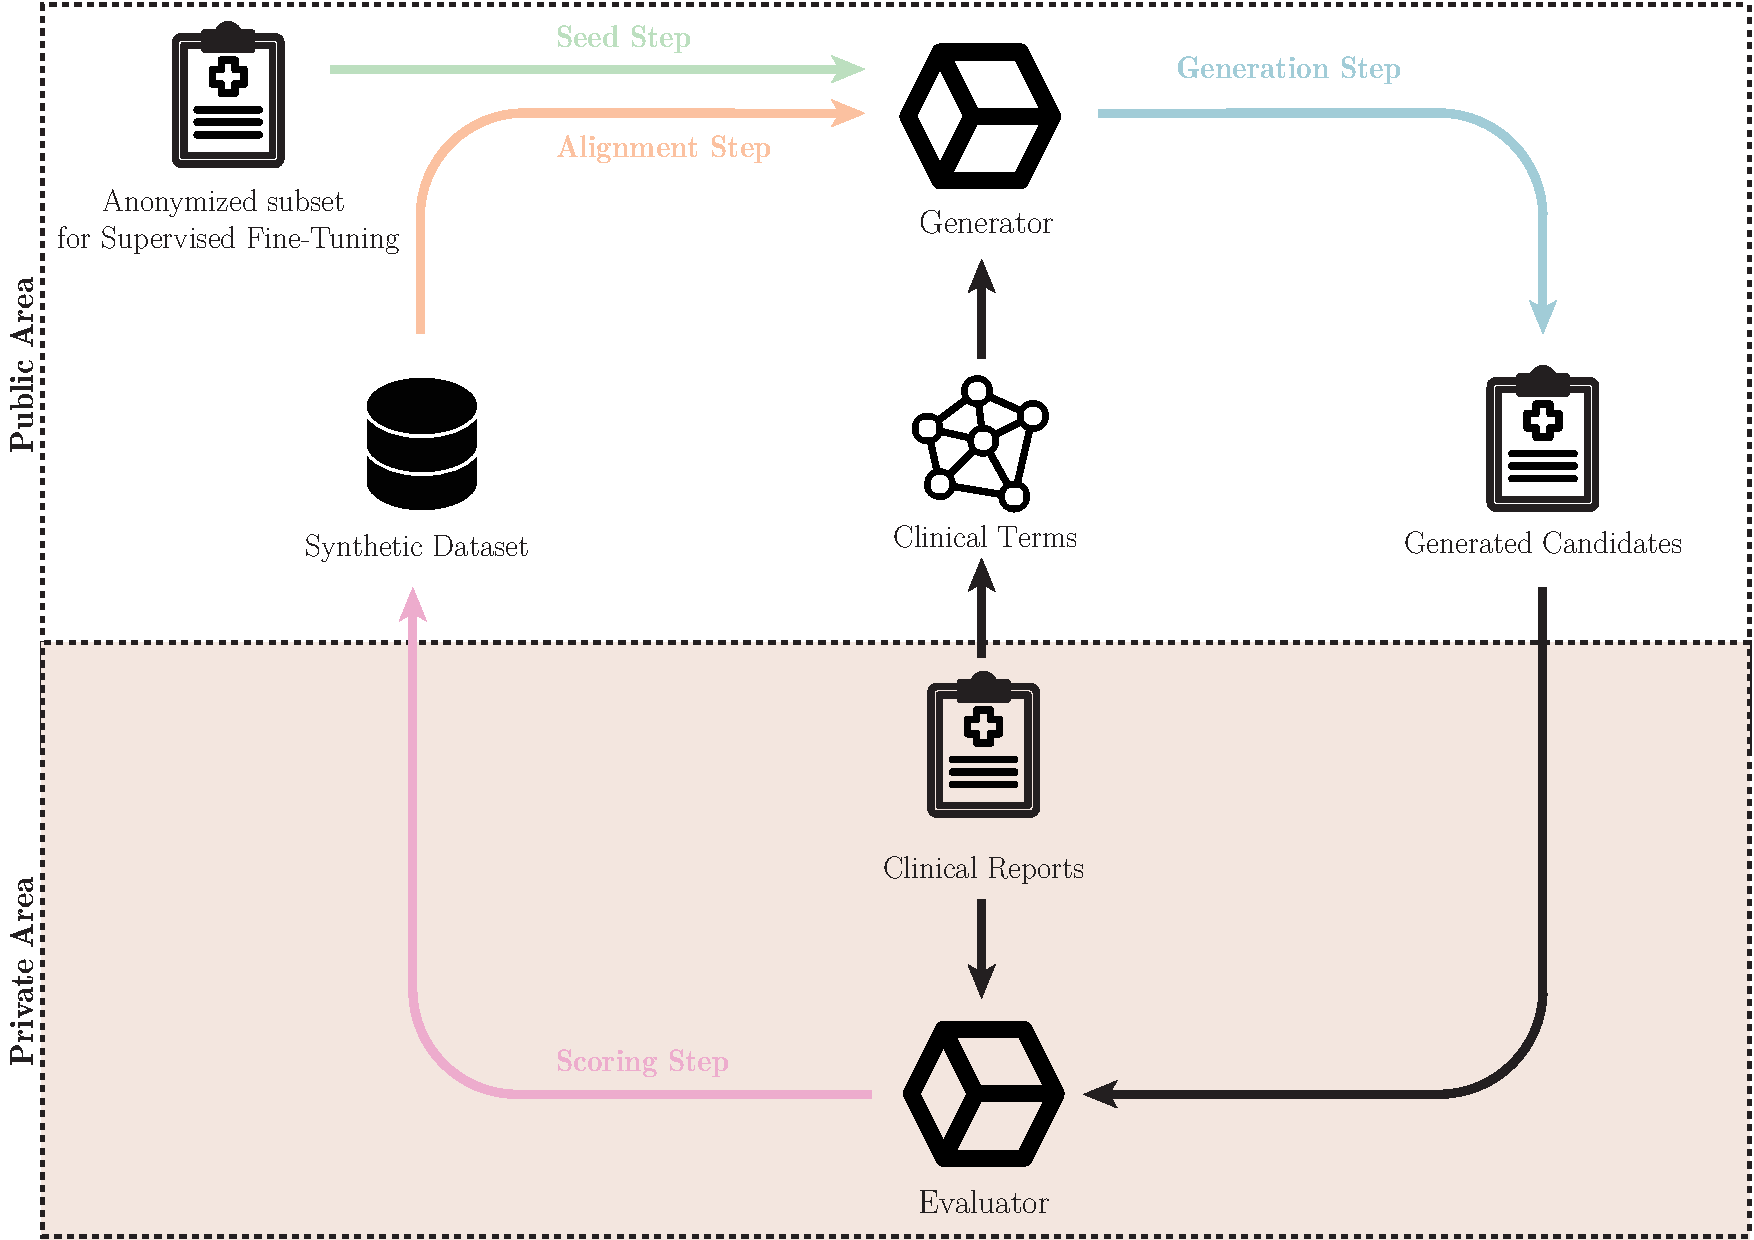
\includegraphics[width=1\textwidth]{figures/synthetic_generation_cl4health_2025/workflow.pdf}
    \caption{workflow of our approach}
    \label{fig:workflow}
\end{figure*}

\subsection{Example Outputs}
\newtcolorbox{modelinput}{colback=blue!5!white,colframe=blue!75!black}
\begin{figure}
\centering
\begin{modelinput}
\verb|<s>[INST]|As a doctor, you must write an original 'History of Present Illness' (HPI) section for a discharge summary.
Your response should capture the essence of a patient's health journey and recent medical experiences, while strictly using all the provided keywords conserving the order.
You must adopt a medical telegraphic style, abbreviated, characterized by concise and direct language.
\\
\textbf{Keywords:} \textit{metastatic, RCC, pancreas, reports, chills, tylenol, reports, rib pain, lying, chills, reports, dark stools, fever, zosyn, headache, contacts, anxious, pain, dysuria, joint pain, rash, hypotensive, asymptomatic, given, lactate, baseline, guaiac, stool, saw, stent, pancreatic, blood, tomorrow, treated, cholangitis, given, sat, ARF, reports, anxious}\verb|[/INST]|
\end{modelinput}
\caption{An example of prompt for the Figures \ref{appendix:ground},\ref{appendix:worst},\ref{appendix:best}}
\label{experiment:prompt}
\end{figure} 

\begin{figure}[!hbt]
    \centering
    \begin{modelinput}
    This is a 67 y.o male with h.o metastatic RCC to the pancreas,
recent ICU course for UGIB (12units pRBCs) who reports sudden
intermittent chills since wednesday for which he took tylenol.
Pt also reports R.side gnawing rib pain, while lying in bed
before the onset of chills. In addition, pt reports dark stools
for the last few days which started after taking "iron pills".
Pt states he went to [**Hospital1 2436**] ED because of a fever of 101.3,
however he felt better and did not want to wait to be seen. He
returned to [**Hospital1 2436**] today and was transferred to [**Hospital1 18**] after
a dose of zosyn, HCT 25. Pt denies headache/dizziness/blurred
vision, URI/cough, sick contacts, CP, +palp when anxious, -abd
pain/n/v/d/brbpr, dysuria/hematuria, joint pain, rash,
paresthesias. \\
. \\
At [**Hospital1 18**], pt found to be hypotensive to 75/40, asymptomatic. He
was given 3L IVF, lactate 6.8. HCT 22.8 from a baseline of 35 a
few weeks ago. He was found to have black, guaiac +stool. GI saw
pt, pt s/p stent to pancreatic ampulla, ?blocked  from blood.
Plan is to transfuse, ERCP tomorrow. ED also treated for
possible cholangitis/sepsis and pt was given dose of vanco.
Vitals 99.2, BP 99/66 HR 88 sat 98% on RA. Access 3PIV's 2,
20's, 18. Pt also found to be in ARF. \\
. \\
Currently, pt reports that he is anxious. \\
.
    \end{modelinput}
    \caption{An example of a ground truth associated with the prompt of Figure~\ref{experiment:prompt}}
    \label{appendix:ground}
\end{figure}

\begin{figure}[!hbt]
\centering
\begin{modelinput}
77 yo M w/ hx of metastatic RCC of the pancreas (pancreo-duodenal \\
mass reports R/o chills since starting [**6-2**] on [**2160-5-18**] (day 7-10 from \\
Hx. He has had fevers with taking tylenol at that time \\
(Ibuprofen 400mg, acetaminophen 650mg PRN for R/o rib pain and \\
steal). On [**2160-5-22**] he was lying in bed and became extremely \\
ill with chills. He reports this started a few minutes ago. Also \\
reports dark stools. His fever is 102F (38.3C), he is on 2g IV \\
zosyn (given IVF 2L NS, as he is V/5) for pneumonia with HC \\
reported by the Wife. He reports severe headache. He is not \\
compliant with PCP but has noticed many recent contacts with \\
his S/M. He is very anxious for relief of pain. He has some \\
dysuria and no joint pain. He has no rash. He is in the ED \\
actively pacing. He is hypotensive. He is BP 90/45 with 3+ pti \\
on his left hand. PRI all his vitals are stable otherwise at \\
BP 92/44 HR 81 RR 14 96 O2 Sat 99% RA. On ABG: pH 7.31, \\
PaCO2 28.1, PaO2 113. As a baseline (was done in ED), guaiac \\
in stool was positive. He was sent to CT with ortho in ED. Saw \\
his PCR [**Last Name (Only) **] [**Date**] [**Time (only) **] 5:15 and showed a 6.2mm x 5.1mm pancreatic \\
tail mass (blood in the head of the pancreas with no dilation \\
distally). He is scheduled for pancreatic stent placement \\
tomorrow. He was treated for acute cholangitis (e.g. given 3L NS \\
and 1g of IVF) and was given 1L NS to help with ARF. He \\
reports that he is more anxious for relief of pain.
\end{modelinput}
\caption{An example of synthetic data generated with Figure \ref{experiment:prompt} with a high \score}
\label{appendix:best}
\end{figure}
